% Options for packages loaded elsewhere
\PassOptionsToPackage{unicode}{hyperref}
\PassOptionsToPackage{hyphens}{url}
%
\documentclass[
]{book}
\usepackage{amsmath,amssymb}
\usepackage{lmodern}
\usepackage{iftex}
\ifPDFTeX
  \usepackage[T1]{fontenc}
  \usepackage[utf8]{inputenc}
  \usepackage{textcomp} % provide euro and other symbols
\else % if luatex or xetex
  \usepackage{unicode-math}
  \defaultfontfeatures{Scale=MatchLowercase}
  \defaultfontfeatures[\rmfamily]{Ligatures=TeX,Scale=1}
\fi
% Use upquote if available, for straight quotes in verbatim environments
\IfFileExists{upquote.sty}{\usepackage{upquote}}{}
\IfFileExists{microtype.sty}{% use microtype if available
  \usepackage[]{microtype}
  \UseMicrotypeSet[protrusion]{basicmath} % disable protrusion for tt fonts
}{}
\makeatletter
\@ifundefined{KOMAClassName}{% if non-KOMA class
  \IfFileExists{parskip.sty}{%
    \usepackage{parskip}
  }{% else
    \setlength{\parindent}{0pt}
    \setlength{\parskip}{6pt plus 2pt minus 1pt}}
}{% if KOMA class
  \KOMAoptions{parskip=half}}
\makeatother
\usepackage{xcolor}
\usepackage{color}
\usepackage{fancyvrb}
\newcommand{\VerbBar}{|}
\newcommand{\VERB}{\Verb[commandchars=\\\{\}]}
\DefineVerbatimEnvironment{Highlighting}{Verbatim}{commandchars=\\\{\}}
% Add ',fontsize=\small' for more characters per line
\usepackage{framed}
\definecolor{shadecolor}{RGB}{248,248,248}
\newenvironment{Shaded}{\begin{snugshade}}{\end{snugshade}}
\newcommand{\AlertTok}[1]{\textcolor[rgb]{0.94,0.16,0.16}{#1}}
\newcommand{\AnnotationTok}[1]{\textcolor[rgb]{0.56,0.35,0.01}{\textbf{\textit{#1}}}}
\newcommand{\AttributeTok}[1]{\textcolor[rgb]{0.77,0.63,0.00}{#1}}
\newcommand{\BaseNTok}[1]{\textcolor[rgb]{0.00,0.00,0.81}{#1}}
\newcommand{\BuiltInTok}[1]{#1}
\newcommand{\CharTok}[1]{\textcolor[rgb]{0.31,0.60,0.02}{#1}}
\newcommand{\CommentTok}[1]{\textcolor[rgb]{0.56,0.35,0.01}{\textit{#1}}}
\newcommand{\CommentVarTok}[1]{\textcolor[rgb]{0.56,0.35,0.01}{\textbf{\textit{#1}}}}
\newcommand{\ConstantTok}[1]{\textcolor[rgb]{0.00,0.00,0.00}{#1}}
\newcommand{\ControlFlowTok}[1]{\textcolor[rgb]{0.13,0.29,0.53}{\textbf{#1}}}
\newcommand{\DataTypeTok}[1]{\textcolor[rgb]{0.13,0.29,0.53}{#1}}
\newcommand{\DecValTok}[1]{\textcolor[rgb]{0.00,0.00,0.81}{#1}}
\newcommand{\DocumentationTok}[1]{\textcolor[rgb]{0.56,0.35,0.01}{\textbf{\textit{#1}}}}
\newcommand{\ErrorTok}[1]{\textcolor[rgb]{0.64,0.00,0.00}{\textbf{#1}}}
\newcommand{\ExtensionTok}[1]{#1}
\newcommand{\FloatTok}[1]{\textcolor[rgb]{0.00,0.00,0.81}{#1}}
\newcommand{\FunctionTok}[1]{\textcolor[rgb]{0.00,0.00,0.00}{#1}}
\newcommand{\ImportTok}[1]{#1}
\newcommand{\InformationTok}[1]{\textcolor[rgb]{0.56,0.35,0.01}{\textbf{\textit{#1}}}}
\newcommand{\KeywordTok}[1]{\textcolor[rgb]{0.13,0.29,0.53}{\textbf{#1}}}
\newcommand{\NormalTok}[1]{#1}
\newcommand{\OperatorTok}[1]{\textcolor[rgb]{0.81,0.36,0.00}{\textbf{#1}}}
\newcommand{\OtherTok}[1]{\textcolor[rgb]{0.56,0.35,0.01}{#1}}
\newcommand{\PreprocessorTok}[1]{\textcolor[rgb]{0.56,0.35,0.01}{\textit{#1}}}
\newcommand{\RegionMarkerTok}[1]{#1}
\newcommand{\SpecialCharTok}[1]{\textcolor[rgb]{0.00,0.00,0.00}{#1}}
\newcommand{\SpecialStringTok}[1]{\textcolor[rgb]{0.31,0.60,0.02}{#1}}
\newcommand{\StringTok}[1]{\textcolor[rgb]{0.31,0.60,0.02}{#1}}
\newcommand{\VariableTok}[1]{\textcolor[rgb]{0.00,0.00,0.00}{#1}}
\newcommand{\VerbatimStringTok}[1]{\textcolor[rgb]{0.31,0.60,0.02}{#1}}
\newcommand{\WarningTok}[1]{\textcolor[rgb]{0.56,0.35,0.01}{\textbf{\textit{#1}}}}
\usepackage{longtable,booktabs,array}
\usepackage{calc} % for calculating minipage widths
% Correct order of tables after \paragraph or \subparagraph
\usepackage{etoolbox}
\makeatletter
\patchcmd\longtable{\par}{\if@noskipsec\mbox{}\fi\par}{}{}
\makeatother
% Allow footnotes in longtable head/foot
\IfFileExists{footnotehyper.sty}{\usepackage{footnotehyper}}{\usepackage{footnote}}
\makesavenoteenv{longtable}
\usepackage{graphicx}
\makeatletter
\def\maxwidth{\ifdim\Gin@nat@width>\linewidth\linewidth\else\Gin@nat@width\fi}
\def\maxheight{\ifdim\Gin@nat@height>\textheight\textheight\else\Gin@nat@height\fi}
\makeatother
% Scale images if necessary, so that they will not overflow the page
% margins by default, and it is still possible to overwrite the defaults
% using explicit options in \includegraphics[width, height, ...]{}
\setkeys{Gin}{width=\maxwidth,height=\maxheight,keepaspectratio}
% Set default figure placement to htbp
\makeatletter
\def\fps@figure{htbp}
\makeatother
\setlength{\emergencystretch}{3em} % prevent overfull lines
\providecommand{\tightlist}{%
  \setlength{\itemsep}{0pt}\setlength{\parskip}{0pt}}
\setcounter{secnumdepth}{5}
\usepackage{booktabs}
\ifLuaTeX
  \usepackage{selnolig}  % disable illegal ligatures
\fi
\usepackage[]{natbib}
\bibliographystyle{plainnat}
\IfFileExists{bookmark.sty}{\usepackage{bookmark}}{\usepackage{hyperref}}
\IfFileExists{xurl.sty}{\usepackage{xurl}}{} % add URL line breaks if available
\urlstyle{same} % disable monospaced font for URLs
\hypersetup{
  pdftitle={Time Series Analysis},
  pdfauthor={Shang Chieh},
  hidelinks,
  pdfcreator={LaTeX via pandoc}}

\title{Time Series Analysis}
\author{Shang Chieh}
\date{2023-05-03}

\usepackage{amsthm}
\newtheorem{theorem}{Theorem}[chapter]
\newtheorem{lemma}{Lemma}[chapter]
\newtheorem{corollary}{Corollary}[chapter]
\newtheorem{proposition}{Proposition}[chapter]
\newtheorem{conjecture}{Conjecture}[chapter]
\theoremstyle{definition}
\newtheorem{definition}{Definition}[chapter]
\theoremstyle{definition}
\newtheorem{example}{Example}[chapter]
\theoremstyle{definition}
\newtheorem{exercise}{Exercise}[chapter]
\theoremstyle{definition}
\newtheorem{hypothesis}{Hypothesis}[chapter]
\theoremstyle{remark}
\newtheorem*{remark}{Remark}
\newtheorem*{solution}{Solution}
\begin{document}
\maketitle

{
\setcounter{tocdepth}{1}
\tableofcontents
}
\hypertarget{about}{%
\chapter{About}\label{about}}

This book is a concise lecture note about \emph{Time Series Analysis}.

The content of this book is from the course Time Series Analysis taught by Chris Bilder. You can check his \href{https://www.youtube.com/@ChrisBilder}{YouTube channel} to get full(and correct) information about this course.

Again, I do \textbf{NOT} own the content of this book. I write this book only for studying. All credits belong to Chris Bilder.

If there is any copyright concerns, I will make this book private ASAP.

\hypertarget{introduction-to-r}{%
\chapter{Introduction to R}\label{introduction-to-r}}

We will go over some of the basic R operations in this chapter.

If you have questions, you should check \href{http://www.chrisbilder.com/stat878/sections.html}{Chris Bilder's website} for full information.

\hypertarget{basic-operation}{%
\section{Basic Operation}\label{basic-operation}}

\begin{Shaded}
\begin{Highlighting}[]
\DecValTok{2}\SpecialCharTok{+}\DecValTok{2}
\end{Highlighting}
\end{Shaded}

\begin{verbatim}
## [1] 4
\end{verbatim}

\begin{Shaded}
\begin{Highlighting}[]
\DecValTok{2}\SpecialCharTok{\^{}}\DecValTok{3}
\end{Highlighting}
\end{Shaded}

\begin{verbatim}
## [1] 8
\end{verbatim}

\begin{Shaded}
\begin{Highlighting}[]
\CommentTok{\# calculate the cdf of std. normal}
\FunctionTok{pnorm}\NormalTok{(}\FloatTok{1.96}\NormalTok{) }\CommentTok{\# 1.96 is the quantile}
\end{Highlighting}
\end{Shaded}

\begin{verbatim}
## [1] 0.9750021
\end{verbatim}

\begin{Shaded}
\begin{Highlighting}[]
\FunctionTok{log}\NormalTok{(}\DecValTok{1}\NormalTok{)}
\end{Highlighting}
\end{Shaded}

\begin{verbatim}
## [1] 0
\end{verbatim}

\begin{Shaded}
\begin{Highlighting}[]
\FunctionTok{sin}\NormalTok{(pi}\SpecialCharTok{/}\DecValTok{2}\NormalTok{)}
\end{Highlighting}
\end{Shaded}

\begin{verbatim}
## [1] 1
\end{verbatim}

\begin{Shaded}
\begin{Highlighting}[]
\DecValTok{3}\SpecialCharTok{/}\DecValTok{4}
\end{Highlighting}
\end{Shaded}

\begin{verbatim}
## [1] 0.75
\end{verbatim}

\begin{Shaded}
\begin{Highlighting}[]
\NormalTok{save }\OtherTok{\textless{}{-}} \DecValTok{2}\SpecialCharTok{+}\DecValTok{2}
\NormalTok{save}
\end{Highlighting}
\end{Shaded}

\begin{verbatim}
## [1] 4
\end{verbatim}

\begin{Shaded}
\begin{Highlighting}[]
\FunctionTok{objects}\NormalTok{()}
\end{Highlighting}
\end{Shaded}

\begin{verbatim}
## [1] "save"
\end{verbatim}

\begin{Shaded}
\begin{Highlighting}[]
\FunctionTok{ls}\NormalTok{()}
\end{Highlighting}
\end{Shaded}

\begin{verbatim}
## [1] "save"
\end{verbatim}

\begin{Shaded}
\begin{Highlighting}[]
\CommentTok{\# quit operaiton}
\CommentTok{\# q() }
\end{Highlighting}
\end{Shaded}

\hypertarget{vectors}{%
\section{Vectors}\label{vectors}}

\begin{Shaded}
\begin{Highlighting}[]
\NormalTok{x }\OtherTok{\textless{}{-}} \FunctionTok{c}\NormalTok{(}\DecValTok{1}\NormalTok{,}\DecValTok{2}\NormalTok{,}\DecValTok{3}\NormalTok{,}\DecValTok{4}\NormalTok{,}\DecValTok{5}\NormalTok{)}
\NormalTok{x}
\end{Highlighting}
\end{Shaded}

\begin{verbatim}
## [1] 1 2 3 4 5
\end{verbatim}

\begin{Shaded}
\begin{Highlighting}[]
\FunctionTok{sd}\NormalTok{(x)}
\end{Highlighting}
\end{Shaded}

\begin{verbatim}
## [1] 1.581139
\end{verbatim}

\begin{Shaded}
\begin{Highlighting}[]
\NormalTok{mysd }\OtherTok{\textless{}{-}} \ControlFlowTok{function}\NormalTok{(x)\{}
  \FunctionTok{cat}\NormalTok{(}\StringTok{" My data }\SpecialCharTok{\textbackslash{}n}\StringTok{"}\NormalTok{, x, }\StringTok{"}\SpecialCharTok{\textbackslash{}n}\StringTok{ has std deviation"}\NormalTok{,}\FunctionTok{sqrt}\NormalTok{(}\FunctionTok{var}\NormalTok{(x)))}
\NormalTok{\}}


\FunctionTok{mysd}\NormalTok{(x)}
\end{Highlighting}
\end{Shaded}

\begin{verbatim}
##  My data 
##  1 2 3 4 5 
##  has std deviation 1.581139
\end{verbatim}

\begin{Shaded}
\begin{Highlighting}[]
\FunctionTok{pnorm}\NormalTok{(}\AttributeTok{q=}\FloatTok{1.96}\NormalTok{, }\AttributeTok{mean=}\FloatTok{1.96}\NormalTok{, }\AttributeTok{sd=}\DecValTok{1}\NormalTok{)}
\end{Highlighting}
\end{Shaded}

\begin{verbatim}
## [1] 0.5
\end{verbatim}

The full syntax for \texttt{pnorm()} is \texttt{pnorm(q,\ mean\ =\ 0,\ sd\ =\ 1,\ lower.tail\ =\ TRUE,\ log.p\ =\ FALSE)}

\begin{Shaded}
\begin{Highlighting}[]
\FunctionTok{pnorm}\NormalTok{(}\AttributeTok{q=}\FunctionTok{c}\NormalTok{(}\SpecialCharTok{{-}}\FloatTok{1.96}\NormalTok{,}\FloatTok{1.96}\NormalTok{))}
\end{Highlighting}
\end{Shaded}

\begin{verbatim}
## [1] 0.0249979 0.9750021
\end{verbatim}

\begin{Shaded}
\begin{Highlighting}[]
\NormalTok{x }\OtherTok{\textless{}{-}} \FunctionTok{c}\NormalTok{(}\FloatTok{3.68}\NormalTok{, }\SpecialCharTok{{-}}\FloatTok{3.63}\NormalTok{, }\FloatTok{0.80}\NormalTok{, }\FloatTok{3.03}\NormalTok{, }\SpecialCharTok{{-}}\FloatTok{9.86}\NormalTok{, }\SpecialCharTok{{-}}\FloatTok{8.66}\NormalTok{, }
    \SpecialCharTok{{-}}\FloatTok{2.38}\NormalTok{, }\FloatTok{8.94}\NormalTok{, }\FloatTok{0.52}\NormalTok{, }\FloatTok{1.25}\NormalTok{) }

\NormalTok{y }\OtherTok{\textless{}{-}} \FunctionTok{c}\NormalTok{(}\FloatTok{0.55}\NormalTok{, }\FloatTok{1.65}\NormalTok{, }\FloatTok{0.98}\NormalTok{, }\SpecialCharTok{{-}}\FloatTok{0.07}\NormalTok{, }\SpecialCharTok{{-}}\FloatTok{0.01}\NormalTok{, }\SpecialCharTok{{-}}\FloatTok{0.31}\NormalTok{, }
    \SpecialCharTok{{-}}\FloatTok{0.34}\NormalTok{, }\SpecialCharTok{{-}}\FloatTok{1.38}\NormalTok{, }\SpecialCharTok{{-}}\FloatTok{1.32}\NormalTok{, }\FloatTok{0.53}\NormalTok{)}

\NormalTok{x}\SpecialCharTok{+}\NormalTok{y}
\end{Highlighting}
\end{Shaded}

\begin{verbatim}
##  [1]  4.23 -1.98  1.78  2.96 -9.87 -8.97 -2.72  7.56 -0.80  1.78
\end{verbatim}

\begin{Shaded}
\begin{Highlighting}[]
\NormalTok{x}\SpecialCharTok{*}\NormalTok{y}
\end{Highlighting}
\end{Shaded}

\begin{verbatim}
##  [1]   2.0240  -5.9895   0.7840  -0.2121   0.0986   2.6846   0.8092 -12.3372
##  [9]  -0.6864   0.6625
\end{verbatim}

\begin{Shaded}
\begin{Highlighting}[]
\FunctionTok{mean}\NormalTok{(x)}
\end{Highlighting}
\end{Shaded}

\begin{verbatim}
## [1] -0.631
\end{verbatim}

\begin{Shaded}
\begin{Highlighting}[]
\NormalTok{x}\SpecialCharTok{{-}}\FunctionTok{mean}\NormalTok{(x)}
\end{Highlighting}
\end{Shaded}

\begin{verbatim}
##  [1]  4.311 -2.999  1.431  3.661 -9.229 -8.029 -1.749  9.571  1.151  1.881
\end{verbatim}

\begin{Shaded}
\begin{Highlighting}[]
\NormalTok{x}\SpecialCharTok{*}\DecValTok{2}
\end{Highlighting}
\end{Shaded}

\begin{verbatim}
##  [1]   7.36  -7.26   1.60   6.06 -19.72 -17.32  -4.76  17.88   1.04   2.50
\end{verbatim}

The element(elt)-wise operation makes our life easier.

\hypertarget{files}{%
\section{Files}\label{files}}

Click \href{http://www.chrisbilder.com/stat878/sections/1/gpa.csv}{gpa.csv} to download the GPA csv file.

Click \href{http://www.chrisbilder.com/stat878/sections/1/gpa.txt}{gpa.txt} to download the GPA txt file.

\begin{Shaded}
\begin{Highlighting}[]
\FunctionTok{getwd}\NormalTok{()}
\end{Highlighting}
\end{Shaded}

\begin{verbatim}
## [1] "/Users/weishangjie/Documents/GitHub/Time_Series_Analysis/Book/Time_Series_Analysis"
\end{verbatim}

\begin{Shaded}
\begin{Highlighting}[]
\NormalTok{gpatxt }\OtherTok{\textless{}{-}} \FunctionTok{read.table}\NormalTok{(}\StringTok{"gpa.txt"}\NormalTok{, }\AttributeTok{header=}\ConstantTok{TRUE}\NormalTok{, }\AttributeTok{sep=}\StringTok{""}\NormalTok{)}
\NormalTok{gpacsv }\OtherTok{\textless{}{-}} \FunctionTok{read.csv}\NormalTok{(}\StringTok{"gpa.csv"}\NormalTok{)}

\CommentTok{\#write.table(x = gpacsv, file = "gpa{-}out1.csv", quote = FALSE, row.names =}
\CommentTok{\#  FALSE, sep  =",")}
\CommentTok{\#write.csv(x = gpacsv, file = "gpa{-}out2.csv")}
\end{Highlighting}
\end{Shaded}

\begin{Shaded}
\begin{Highlighting}[]
\NormalTok{gpacsv}\SpecialCharTok{$}\NormalTok{HSGPA}
\end{Highlighting}
\end{Shaded}

\begin{verbatim}
##  [1] 3.04 2.35 2.70 2.55 2.83 4.32 3.39 2.32 2.69 2.83 2.39 3.65 2.85 3.83 2.22
## [16] 1.98 2.88 4.00 2.28 2.88
\end{verbatim}

\begin{Shaded}
\begin{Highlighting}[]
\NormalTok{gpacsv}\SpecialCharTok{$}\NormalTok{CollegeGPA}
\end{Highlighting}
\end{Shaded}

\begin{verbatim}
##  [1] 3.10 2.30 3.00 2.45 2.50 3.70 3.40 2.60 2.80 3.60 2.00 2.90 3.30 3.20 2.80
## [16] 2.40 2.60 3.80 2.20 2.60
\end{verbatim}

\begin{Shaded}
\begin{Highlighting}[]
\NormalTok{gpacsv[}\DecValTok{1}\NormalTok{,}\DecValTok{1}\NormalTok{] }\CommentTok{\# [row, col]}
\end{Highlighting}
\end{Shaded}

\begin{verbatim}
## [1] 3.04
\end{verbatim}

\begin{Shaded}
\begin{Highlighting}[]
\NormalTok{gpacsv[,}\DecValTok{1}\NormalTok{]}
\end{Highlighting}
\end{Shaded}

\begin{verbatim}
##  [1] 3.04 2.35 2.70 2.55 2.83 4.32 3.39 2.32 2.69 2.83 2.39 3.65 2.85 3.83 2.22
## [16] 1.98 2.88 4.00 2.28 2.88
\end{verbatim}

\begin{Shaded}
\begin{Highlighting}[]
\NormalTok{gpacsv[}\FunctionTok{c}\NormalTok{(}\DecValTok{1}\NormalTok{,}\DecValTok{3}\NormalTok{,}\DecValTok{5}\NormalTok{),}\DecValTok{2}\NormalTok{]}
\end{Highlighting}
\end{Shaded}

\begin{verbatim}
## [1] 3.1 3.0 2.5
\end{verbatim}

\begin{Shaded}
\begin{Highlighting}[]
\NormalTok{gpacsv[,}\StringTok{"HSGPA"}\NormalTok{]}
\end{Highlighting}
\end{Shaded}

\begin{verbatim}
##  [1] 3.04 2.35 2.70 2.55 2.83 4.32 3.39 2.32 2.69 2.83 2.39 3.65 2.85 3.83 2.22
## [16] 1.98 2.88 4.00 2.28 2.88
\end{verbatim}

\begin{Shaded}
\begin{Highlighting}[]
\FunctionTok{summary}\NormalTok{(gpacsv)}
\end{Highlighting}
\end{Shaded}

\begin{verbatim}
##      HSGPA         CollegeGPA   
##  Min.   :1.980   Min.   :2.000  
##  1st Qu.:2.380   1st Qu.:2.487  
##  Median :2.830   Median :2.800  
##  Mean   :2.899   Mean   :2.862  
##  3rd Qu.:3.127   3rd Qu.:3.225  
##  Max.   :4.320   Max.   :3.800
\end{verbatim}

\begin{Shaded}
\begin{Highlighting}[]
\FunctionTok{names}\NormalTok{(gpacsv)}
\end{Highlighting}
\end{Shaded}

\begin{verbatim}
## [1] "HSGPA"      "CollegeGPA"
\end{verbatim}

\begin{Shaded}
\begin{Highlighting}[]
\FunctionTok{plot}\NormalTok{(}\AttributeTok{x =}\NormalTok{ gpacsv}\SpecialCharTok{$}\NormalTok{HSGPA, }\AttributeTok{y =}\NormalTok{ gpacsv}\SpecialCharTok{$}\NormalTok{CollegeGPA,}
     \AttributeTok{xlab =} \StringTok{"HS GPA"}\NormalTok{, }\AttributeTok{ylab =} \StringTok{"College GPA"}\NormalTok{, }
     \AttributeTok{main =} \StringTok{"College GPA vs. HS GPA"}\NormalTok{, }
     \AttributeTok{xlim =} \FunctionTok{c}\NormalTok{(}\DecValTok{0}\NormalTok{,}\FloatTok{4.5}\NormalTok{), }\AttributeTok{ylim =} \FunctionTok{c}\NormalTok{(}\DecValTok{0}\NormalTok{,}\FloatTok{4.5}\NormalTok{), }\AttributeTok{col =} \StringTok{"red"}\NormalTok{, }
    \AttributeTok{pch =} \DecValTok{1}\NormalTok{, }\AttributeTok{cex =} \FloatTok{1.0}\NormalTok{, }\AttributeTok{panel.first =} \FunctionTok{grid}\NormalTok{(}\AttributeTok{col =} \StringTok{"gray"}\NormalTok{, lty }
    \OtherTok{=} \StringTok{"dotted"}\NormalTok{))}
\end{Highlighting}
\end{Shaded}

\includegraphics{01-Introduction-to-R_files/figure-latex/unnamed-chunk-27-1.pdf}
The \texttt{plot()} function creates a two dimensional plot of data.

Here are descriptions of its arguments:

\begin{itemize}
\item
  x specifies what is plotted for the x-axis.
\item
  y specifies what is plotted for the y-axis.
\item
  xlab and ylab specify the x-axis and y-axis labels, respectively.
\item
  main specifies the main title of the plot.
\item
  xlim and ylim specify the x-axis and y-axis limits, respectively.

  \begin{itemize}
  \tightlist
  \item
    Notice the use of the c() function.
  \end{itemize}
\item
  col specifies the color of the plotting points.

  \begin{itemize}
  \tightlist
  \item
    Run the \texttt{colors()} function to see what possible colors can be used.
  \item
    Also, you can see \href{https://github.com/EarlGlynn/colorchart/wiki/Color-Chart-in-R}{Here} for the colors from colors().
  \end{itemize}
\item
  \texttt{pch} specifies the plotting characters.
\item
  \texttt{cex}specifies the height of the plotting characters.
  The value 1.0 is the default.
\item
  \texttt{panel.first\ =\ grid()} specifies grid lines will be plotted.
\item
  The line types can be specified as follows:
  \texttt{1=solid,\ 2=dashed,\ 3=dotted,\ 4=dotdash,\ 5=longdash,\ 6=twodash} or as one of the character strings \texttt{"blank",\ "solid",\ "dashed",\ "dotted",\ \ "dotdash",\ "longdash"}, or \texttt{"twodash"}.\\
  These line type specifications can be used in other functions.\\
\item
  The \texttt{par()}(parameter) function's Help contains more information about the different plotting options!
\end{itemize}

\hypertarget{regression}{%
\section{Regression}\label{regression}}

Our model is:\[CollegeGPA=\beta_0+\beta_1HSGPA+\epsilon\]

\begin{Shaded}
\begin{Highlighting}[]
\NormalTok{mod.fit }\OtherTok{\textless{}{-}} \FunctionTok{lm}\NormalTok{(}\AttributeTok{formula=}\NormalTok{ CollegeGPA}\SpecialCharTok{\textasciitilde{}}\NormalTok{ HSGPA, }\AttributeTok{data=}\NormalTok{gpacsv)}
\NormalTok{mod.fit}
\end{Highlighting}
\end{Shaded}

\begin{verbatim}
## 
## Call:
## lm(formula = CollegeGPA ~ HSGPA, data = gpacsv)
## 
## Coefficients:
## (Intercept)        HSGPA  
##      1.0869       0.6125
\end{verbatim}

\begin{Shaded}
\begin{Highlighting}[]
\FunctionTok{names}\NormalTok{(mod.fit)}
\end{Highlighting}
\end{Shaded}

\begin{verbatim}
##  [1] "coefficients"  "residuals"     "effects"       "rank"         
##  [5] "fitted.values" "assign"        "qr"            "df.residual"  
##  [9] "xlevels"       "call"          "terms"         "model"
\end{verbatim}

\begin{Shaded}
\begin{Highlighting}[]
\NormalTok{mod.fit}\SpecialCharTok{$}\NormalTok{coefficients}
\end{Highlighting}
\end{Shaded}

\begin{verbatim}
## (Intercept)       HSGPA 
##   1.0868795   0.6124941
\end{verbatim}

\begin{Shaded}
\begin{Highlighting}[]
\FunctionTok{round}\NormalTok{(mod.fit}\SpecialCharTok{$}\NormalTok{residuals[}\DecValTok{1}\SpecialCharTok{:}\DecValTok{5}\NormalTok{],}\DecValTok{2}\NormalTok{)}
\end{Highlighting}
\end{Shaded}

\begin{verbatim}
##     1     2     3     4     5 
##  0.15 -0.23  0.26 -0.20 -0.32
\end{verbatim}

\begin{Shaded}
\begin{Highlighting}[]
\FunctionTok{library}\NormalTok{(tidyverse)}
\end{Highlighting}
\end{Shaded}

\begin{verbatim}
## -- Attaching core tidyverse packages ------------------------ tidyverse 2.0.0 --
## v dplyr     1.1.1     v readr     2.1.4
## v forcats   1.0.0     v stringr   1.5.0
## v ggplot2   3.4.1     v tibble    3.2.1
## v lubridate 1.9.2     v tidyr     1.3.0
## v purrr     1.0.1     
## -- Conflicts ------------------------------------------ tidyverse_conflicts() --
## x dplyr::filter() masks stats::filter()
## x dplyr::lag()    masks stats::lag()
## i Use the conflicted package (<http://conflicted.r-lib.org/>) to force all conflicts to become errors
\end{verbatim}

\begin{Shaded}
\begin{Highlighting}[]
\NormalTok{save.fit }\OtherTok{\textless{}{-}} \FunctionTok{data.frame}\NormalTok{(gpacsv, }\AttributeTok{C.GPA.hat =} 
    \FunctionTok{round}\NormalTok{(mod.fit}\SpecialCharTok{$}\NormalTok{fitted.values,}\DecValTok{2}\NormalTok{), }\AttributeTok{residuals =} 
    \FunctionTok{round}\NormalTok{(mod.fit}\SpecialCharTok{$}\NormalTok{residuals,}\DecValTok{2}\NormalTok{))}

\NormalTok{save.fit }\SpecialCharTok{\%\textgreater{}\%} \FunctionTok{head}\NormalTok{()}
\end{Highlighting}
\end{Shaded}

\begin{verbatim}
##   HSGPA CollegeGPA C.GPA.hat residuals
## 1  3.04       3.10      2.95      0.15
## 2  2.35       2.30      2.53     -0.23
## 3  2.70       3.00      2.74      0.26
## 4  2.55       2.45      2.65     -0.20
## 5  2.83       2.50      2.82     -0.32
## 6  4.32       3.70      3.73     -0.03
\end{verbatim}

\begin{Shaded}
\begin{Highlighting}[]
\FunctionTok{summary}\NormalTok{(mod.fit)}
\end{Highlighting}
\end{Shaded}

\begin{verbatim}
## 
## Call:
## lm(formula = CollegeGPA ~ HSGPA, data = gpacsv)
## 
## Residuals:
##      Min       1Q   Median       3Q      Max 
## -0.55074 -0.25086  0.01633  0.24242  0.77976 
## 
## Coefficients:
##             Estimate Std. Error t value Pr(>|t|)    
## (Intercept)   1.0869     0.3666   2.965 0.008299 ** 
## HSGPA         0.6125     0.1237   4.953 0.000103 ***
## ---
## Signif. codes:  0 '***' 0.001 '**' 0.01 '*' 0.05 '.' 0.1 ' ' 1
## 
## Residual standard error: 0.3437 on 18 degrees of freedom
## Multiple R-squared:  0.5768, Adjusted R-squared:  0.5533 
## F-statistic: 24.54 on 1 and 18 DF,  p-value: 0.0001027
\end{verbatim}

\begin{Shaded}
\begin{Highlighting}[]
\FunctionTok{class}\NormalTok{(mod.fit)}
\end{Highlighting}
\end{Shaded}

\begin{verbatim}
## [1] "lm"
\end{verbatim}

Hence, our estimated regression model is\[ \hat{collge.GPA}=\hat{\beta_0}+\hat{\beta_1}HS.GPA
=1.0869+0.6125HS.GPA\]

\begin{Shaded}
\begin{Highlighting}[]
\CommentTok{\# Open a new graphics window }
\CommentTok{\# device new}
\FunctionTok{dev.new}\NormalTok{(}\AttributeTok{width =} \DecValTok{8}\NormalTok{, }\AttributeTok{height =} \DecValTok{6}\NormalTok{, }\AttributeTok{pointsize =} \DecValTok{10}\NormalTok{)}


\CommentTok{\# 1 row and 2 columns of plots}
\FunctionTok{par}\NormalTok{(}\AttributeTok{mfrow =} \FunctionTok{c}\NormalTok{(}\DecValTok{1}\NormalTok{,}\DecValTok{2}\NormalTok{))}
\CommentTok{\# par= graphic parameter}
\CommentTok{\# mfrow= make a frame by row}

\CommentTok{\# Same scatter plot as before}
\FunctionTok{plot}\NormalTok{(}\AttributeTok{x =}\NormalTok{ gpacsv}\SpecialCharTok{$}\NormalTok{HSGPA, }\AttributeTok{y =}\NormalTok{ gpacsv}\SpecialCharTok{$}\NormalTok{CollegeGPA, }\AttributeTok{xlab =} \StringTok{"HS }
\StringTok{    GPA"}\NormalTok{, }\AttributeTok{ylab =} \StringTok{"College GPA"}\NormalTok{, }\AttributeTok{main =} \StringTok{"College GPA vs. }
\StringTok{    HS GPA"}\NormalTok{, }\AttributeTok{xlim =} \FunctionTok{c}\NormalTok{(}\DecValTok{0}\NormalTok{,}\FloatTok{4.5}\NormalTok{), }\AttributeTok{ylim =} \FunctionTok{c}\NormalTok{(}\DecValTok{0}\NormalTok{,}\FloatTok{4.5}\NormalTok{), }\AttributeTok{col =} 
    \StringTok{"red"}\NormalTok{, }\AttributeTok{pch =} \DecValTok{1}\NormalTok{, }\AttributeTok{cex =} \FloatTok{1.0}\NormalTok{, }\AttributeTok{panel.first =} \FunctionTok{grid}\NormalTok{(}\AttributeTok{col =} 
    \StringTok{"gray"}\NormalTok{, }\AttributeTok{lty =} \StringTok{"dotted"}\NormalTok{))}
    
\CommentTok{\# Puts the line y = a + bx on the plot}
\FunctionTok{abline}\NormalTok{(}\AttributeTok{a =}\NormalTok{ mod.fit}\SpecialCharTok{$}\NormalTok{coefficients[}\DecValTok{1}\NormalTok{], }\AttributeTok{b =} 
\NormalTok{    mod.fit}\SpecialCharTok{$}\NormalTok{coefficients[}\DecValTok{2}\NormalTok{], }\AttributeTok{lty =} \StringTok{"solid"}\NormalTok{, }\AttributeTok{col =} 
    \StringTok{"blue"}\NormalTok{, }\AttributeTok{lwd =} \DecValTok{2}\NormalTok{)}
\end{Highlighting}
\end{Shaded}

\begin{Shaded}
\begin{Highlighting}[]
\CommentTok{\# Same scatter plot as before}
\FunctionTok{plot}\NormalTok{(}\AttributeTok{x =}\NormalTok{ gpacsv}\SpecialCharTok{$}\NormalTok{HSGPA, }\AttributeTok{y =}\NormalTok{ gpacsv}\SpecialCharTok{$}\NormalTok{CollegeGPA, }\AttributeTok{xlab =} \StringTok{"HS }
\StringTok{    GPA"}\NormalTok{, }\AttributeTok{ylab =} \StringTok{"College GPA"}\NormalTok{, }\AttributeTok{main =} \StringTok{"College GPA vs. }
\StringTok{    HS GPA"}\NormalTok{, }\AttributeTok{xlim =} \FunctionTok{c}\NormalTok{(}\DecValTok{0}\NormalTok{,}\FloatTok{4.5}\NormalTok{), }\AttributeTok{ylim =} \FunctionTok{c}\NormalTok{(}\DecValTok{0}\NormalTok{,}\FloatTok{4.5}\NormalTok{), }\AttributeTok{col =} 
    \StringTok{"red"}\NormalTok{, }\AttributeTok{pch =} \DecValTok{1}\NormalTok{, }\AttributeTok{cex =} \FloatTok{1.0}\NormalTok{, }\AttributeTok{panel.first =} \FunctionTok{grid}\NormalTok{(}\AttributeTok{col =} 
    \StringTok{"gray"}\NormalTok{, }\AttributeTok{lty =} \StringTok{"dotted"}\NormalTok{))}


\CommentTok{\# Add line}
\CommentTok{\# expr= math expression}
\FunctionTok{curve}\NormalTok{(}\AttributeTok{expr =}\NormalTok{ mod.fit}\SpecialCharTok{$}\NormalTok{coefficients[}\DecValTok{1}\NormalTok{] }\SpecialCharTok{+} 
\NormalTok{    mod.fit}\SpecialCharTok{$}\NormalTok{coefficients[}\DecValTok{2}\NormalTok{]}\SpecialCharTok{*}\NormalTok{x, }
    \AttributeTok{xlim =} \FunctionTok{c}\NormalTok{(}\FunctionTok{min}\NormalTok{(gpacsv}\SpecialCharTok{$}\NormalTok{HSGPA),}\FunctionTok{max}\NormalTok{(gpacsv}\SpecialCharTok{$}\NormalTok{HSGPA)), }
    \AttributeTok{col=} \StringTok{"blue"}\NormalTok{, }\AttributeTok{add =} \ConstantTok{TRUE}\NormalTok{, }\AttributeTok{lwd =} \DecValTok{2}\NormalTok{)}


\CommentTok{\# Draw a line from (x0, y0) to (x1, y1)}
  \FunctionTok{segments}\NormalTok{(}\AttributeTok{x0 =} \FunctionTok{min}\NormalTok{(gpacsv}\SpecialCharTok{$}\NormalTok{HSGPA), }\AttributeTok{y0 =}\NormalTok{ mod.fit}\SpecialCharTok{$}\NormalTok{coefficients[}\DecValTok{1}\NormalTok{] }\SpecialCharTok{+}\NormalTok{ mod.fit}\SpecialCharTok{$}\NormalTok{coefficients[}\DecValTok{2}\NormalTok{]}\SpecialCharTok{*}\FunctionTok{min}\NormalTok{(gpacsv}\SpecialCharTok{$}\NormalTok{HSGPA),}
           \AttributeTok{x1 =} \FunctionTok{max}\NormalTok{(gpacsv}\SpecialCharTok{$}\NormalTok{HSGPA), }\AttributeTok{y1 =}\NormalTok{ mod.fit}\SpecialCharTok{$}\NormalTok{coefficients[}\DecValTok{1}\NormalTok{] }\SpecialCharTok{+}\NormalTok{ mod.fit}\SpecialCharTok{$}\NormalTok{coefficients[}\DecValTok{2}\NormalTok{]}\SpecialCharTok{*}\FunctionTok{max}\NormalTok{(gpacsv}\SpecialCharTok{$}\NormalTok{HSGPA),}
           \AttributeTok{lty =} \DecValTok{1}\NormalTok{, }\AttributeTok{col =} \StringTok{"blue"}\NormalTok{, }\AttributeTok{lwd =} \DecValTok{2}\NormalTok{)}
\end{Highlighting}
\end{Shaded}

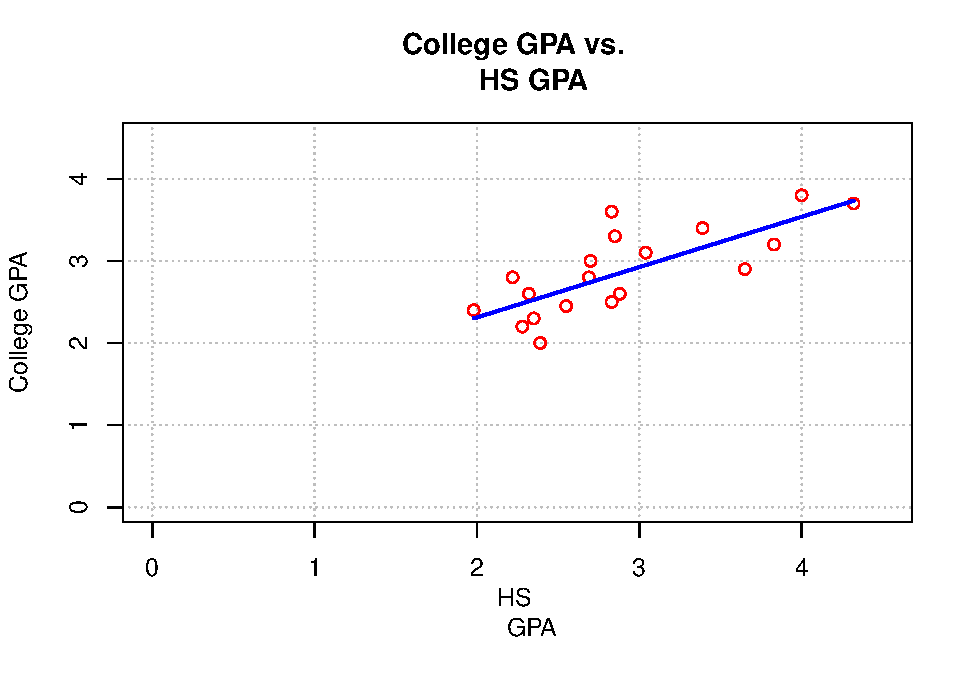
\includegraphics{01-Introduction-to-R_files/figure-latex/unnamed-chunk-35-1.pdf}

\begin{itemize}
\item
  The \texttt{dev.new()} function can be used to open a new plotting window.
\item
  The \texttt{abline()} function can be used to draw straight lines on a plot. In the format used here, the line y = a + bx was drawn where a was the (intercept) and b was the (slope).
\item
  In the second plot, the curve() function was used to draw the line on the plot. This was done to have the line within the range of the high school GPA values.
\end{itemize}

Let's use function to automate what we have done.

\begin{Shaded}
\begin{Highlighting}[]
\NormalTok{my.reg.func }\OtherTok{\textless{}{-}} \ControlFlowTok{function}\NormalTok{(x, y, data) \{}

    \CommentTok{\# Fit the simple linear regression model and save the results in mod.fit}
\NormalTok{    mod.fit }\OtherTok{\textless{}{-}} \FunctionTok{lm}\NormalTok{(}\AttributeTok{formula =}\NormalTok{ y }\SpecialCharTok{\textasciitilde{}}\NormalTok{ x, }\AttributeTok{data =}\NormalTok{ data)}

    \CommentTok{\#Open a new graphics window {-} do not need to}
    \FunctionTok{dev.new}\NormalTok{(}\AttributeTok{width =} \DecValTok{6}\NormalTok{, }\AttributeTok{height =} \DecValTok{6}\NormalTok{, }\AttributeTok{pointsize =} \DecValTok{10}\NormalTok{)}

    \CommentTok{\# Same scatter plot as before}
    \FunctionTok{plot}\NormalTok{(}\AttributeTok{x =}\NormalTok{ x, }\AttributeTok{y =}\NormalTok{ y, }\AttributeTok{xlab =} \StringTok{"x"}\NormalTok{, }\AttributeTok{ylab =} \StringTok{"y"}\NormalTok{, }\AttributeTok{main =} \StringTok{"y vs. x"}\NormalTok{, }\AttributeTok{panel.first=}\FunctionTok{grid}\NormalTok{(}\AttributeTok{col =} \StringTok{"gray"}\NormalTok{, }\AttributeTok{lty =} 
      \StringTok{"dotted"}\NormalTok{))}

    \CommentTok{\# Plot model}
    \FunctionTok{curve}\NormalTok{(}\AttributeTok{expr =}\NormalTok{ mod.fit}\SpecialCharTok{$}\NormalTok{coefficients[}\DecValTok{1}\NormalTok{] }\SpecialCharTok{+} 
\NormalTok{      mod.fit}\SpecialCharTok{$}\NormalTok{coefficients[}\DecValTok{2}\NormalTok{]}\SpecialCharTok{*}\NormalTok{x, }\AttributeTok{xlim =} \FunctionTok{c}\NormalTok{(}\FunctionTok{min}\NormalTok{(x),}\FunctionTok{max}\NormalTok{(x)), }
      \AttributeTok{col =} \StringTok{"blue"}\NormalTok{, }\AttributeTok{add =} \ConstantTok{TRUE}\NormalTok{)}
    
    \FunctionTok{segments}\NormalTok{(}\AttributeTok{x0 =} \FunctionTok{min}\NormalTok{(x), }\AttributeTok{y0 =}\NormalTok{ mod.fit}\SpecialCharTok{$}\NormalTok{coefficients[}\DecValTok{1}\NormalTok{] }\SpecialCharTok{+}\NormalTok{ mod.fit}\SpecialCharTok{$}\NormalTok{coefficients[}\DecValTok{2}\NormalTok{]}\SpecialCharTok{*}\FunctionTok{min}\NormalTok{(x),}
             \AttributeTok{x1 =} \FunctionTok{max}\NormalTok{(x), }\AttributeTok{y1 =}\NormalTok{ mod.fit}\SpecialCharTok{$}\NormalTok{coefficients[}\DecValTok{1}\NormalTok{] }\SpecialCharTok{+}\NormalTok{ mod.fit}\SpecialCharTok{$}\NormalTok{coefficients[}\DecValTok{2}\NormalTok{]}\SpecialCharTok{*}\FunctionTok{max}\NormalTok{(x),}
             \AttributeTok{lty =} \DecValTok{1}\NormalTok{, }\AttributeTok{col =} \StringTok{"blue"}\NormalTok{, }\AttributeTok{lwd =} \DecValTok{2}\NormalTok{)}

    \CommentTok{\# This is the object returned}
\NormalTok{    mod.fit}
\NormalTok{  \}}
\end{Highlighting}
\end{Shaded}

\begin{Shaded}
\begin{Highlighting}[]
\NormalTok{save.it }\OtherTok{\textless{}{-}} \FunctionTok{my.reg.func}\NormalTok{(}\AttributeTok{x =}\NormalTok{ gpacsv}\SpecialCharTok{$}\NormalTok{HSGPA, }\AttributeTok{y =} 
\NormalTok{    gpacsv}\SpecialCharTok{$}\NormalTok{CollegeGPA, }\AttributeTok{data =}\NormalTok{ gpacsv)}
\end{Highlighting}
\end{Shaded}

To get specific x-axis or y-axis tick marks on a plot, use the \texttt{axis()} function. For example,

\begin{Shaded}
\begin{Highlighting}[]
\CommentTok{\#Note that xaxt = "n" tells R to not give any labels on the }
\CommentTok{\#  x{-}axis (yaxt = "n" works for y{-}axis)}
\FunctionTok{plot}\NormalTok{(}\AttributeTok{x =}\NormalTok{ gpacsv}\SpecialCharTok{$}\NormalTok{HSGPA, }\AttributeTok{y =}\NormalTok{ gpacsv}\SpecialCharTok{$}\NormalTok{CollegeGPA, }\AttributeTok{xlab =} \StringTok{"HS GPA"}\NormalTok{, }
     \AttributeTok{ylab =} \StringTok{"College GPA"}\NormalTok{, }\AttributeTok{main =} \StringTok{"College GPA vs. HS GPA"}\NormalTok{, }
     \AttributeTok{xaxt =} \StringTok{"n"}\NormalTok{, }\AttributeTok{xlim =} \FunctionTok{c}\NormalTok{(}\DecValTok{0}\NormalTok{, }\FloatTok{4.5}\NormalTok{), }\AttributeTok{ylim =} \FunctionTok{c}\NormalTok{(}\DecValTok{0}\NormalTok{, }\FloatTok{4.5}\NormalTok{), }\AttributeTok{col =} 
     \StringTok{"red"}\NormalTok{, }\AttributeTok{pch =} \DecValTok{1}\NormalTok{)}
\end{Highlighting}
\end{Shaded}

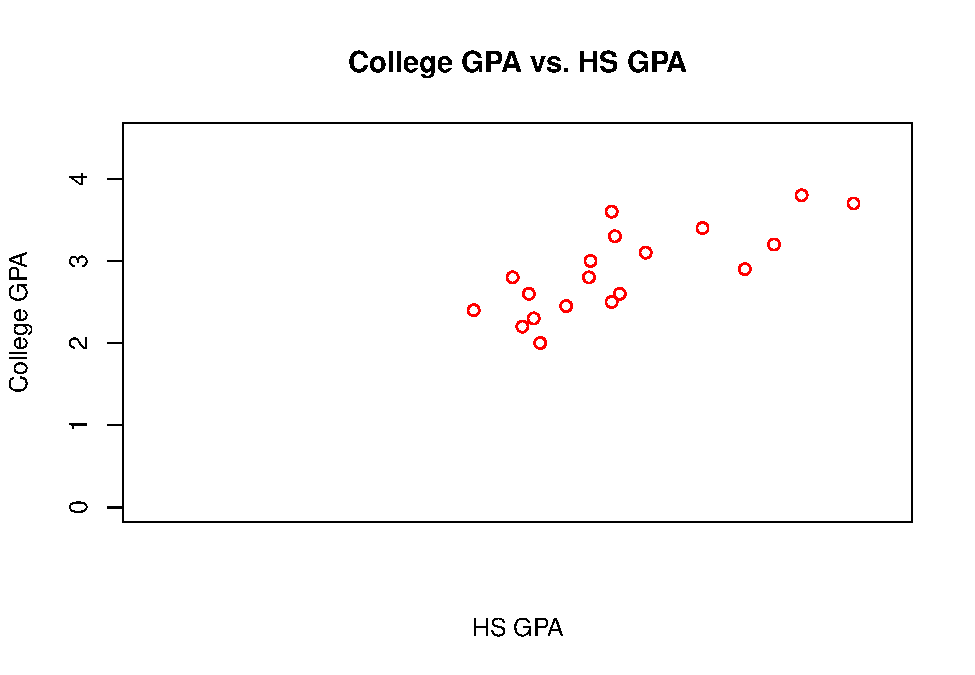
\includegraphics{01-Introduction-to-R_files/figure-latex/unnamed-chunk-38-1.pdf}

\begin{Shaded}
\begin{Highlighting}[]
\FunctionTok{plot}\NormalTok{(}\AttributeTok{x =}\NormalTok{ gpacsv}\SpecialCharTok{$}\NormalTok{HSGPA, }\AttributeTok{y =}\NormalTok{ gpacsv}\SpecialCharTok{$}\NormalTok{CollegeGPA, }\AttributeTok{xlab =} \StringTok{"HS GPA"}\NormalTok{, }
     \AttributeTok{ylab =} \StringTok{"College GPA"}\NormalTok{, }\AttributeTok{main =} \StringTok{"College GPA vs. HS GPA"}\NormalTok{, }
     \AttributeTok{xaxt =} \StringTok{"n"}\NormalTok{, }\AttributeTok{xlim =} \FunctionTok{c}\NormalTok{(}\DecValTok{0}\NormalTok{, }\FloatTok{4.5}\NormalTok{), }\AttributeTok{ylim =} \FunctionTok{c}\NormalTok{(}\DecValTok{0}\NormalTok{, }\FloatTok{4.5}\NormalTok{), }\AttributeTok{col =} 
     \StringTok{"red"}\NormalTok{, }\AttributeTok{pch =} \DecValTok{1}\NormalTok{)}
     
\CommentTok{\#Major tick marks}
\FunctionTok{axis}\NormalTok{(}\AttributeTok{side =} \DecValTok{1}\NormalTok{, }\AttributeTok{at =} \FunctionTok{seq}\NormalTok{(}\AttributeTok{from =} \DecValTok{0}\NormalTok{, }\AttributeTok{to =} \FloatTok{4.5}\NormalTok{, }\AttributeTok{by =} \FloatTok{0.5}\NormalTok{)) }
\end{Highlighting}
\end{Shaded}

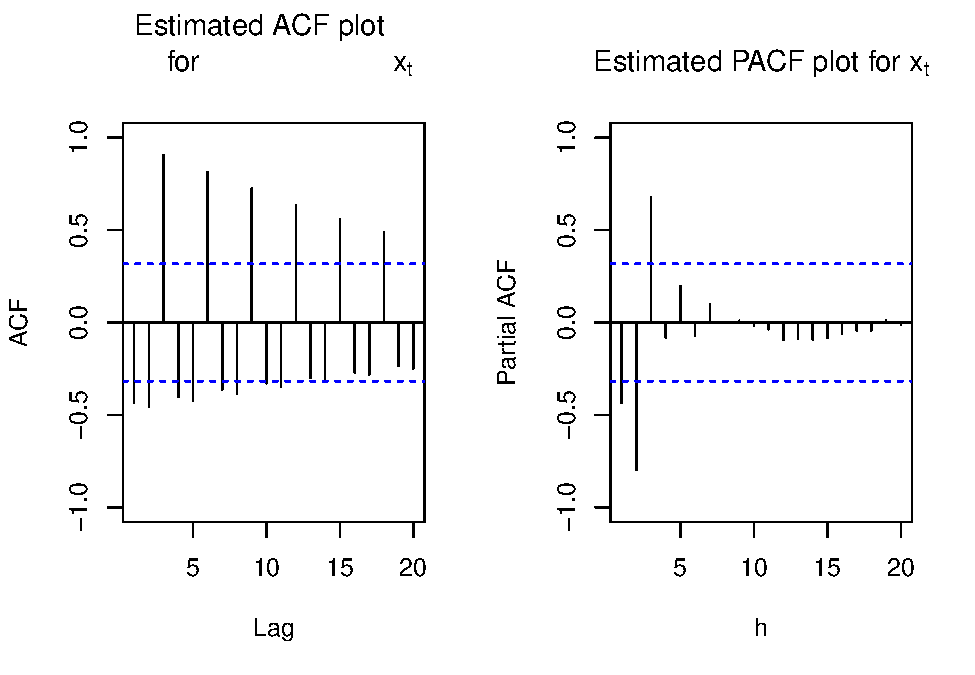
\includegraphics{01-Introduction-to-R_files/figure-latex/unnamed-chunk-39-1.pdf}

\begin{Shaded}
\begin{Highlighting}[]
\FunctionTok{plot}\NormalTok{(}\AttributeTok{x =}\NormalTok{ gpacsv}\SpecialCharTok{$}\NormalTok{HSGPA, }\AttributeTok{y =}\NormalTok{ gpacsv}\SpecialCharTok{$}\NormalTok{CollegeGPA, }\AttributeTok{xlab =} \StringTok{"HS GPA"}\NormalTok{, }
     \AttributeTok{ylab =} \StringTok{"College GPA"}\NormalTok{, }\AttributeTok{main =} \StringTok{"College GPA vs. HS GPA"}\NormalTok{, }
     \AttributeTok{xaxt =} \StringTok{"n"}\NormalTok{, }\AttributeTok{xlim =} \FunctionTok{c}\NormalTok{(}\DecValTok{0}\NormalTok{, }\FloatTok{4.5}\NormalTok{), }\AttributeTok{ylim =} \FunctionTok{c}\NormalTok{(}\DecValTok{0}\NormalTok{, }\FloatTok{4.5}\NormalTok{), }\AttributeTok{col =} 
     \StringTok{"red"}\NormalTok{, }\AttributeTok{pch =} \DecValTok{1}\NormalTok{)}
     
\CommentTok{\#Major tick marks}
\FunctionTok{axis}\NormalTok{(}\AttributeTok{side =} \DecValTok{1}\NormalTok{, }\AttributeTok{at =} \FunctionTok{seq}\NormalTok{(}\AttributeTok{from =} \DecValTok{0}\NormalTok{, }\AttributeTok{to =} \FloatTok{4.5}\NormalTok{, }\AttributeTok{by =} \FloatTok{0.5}\NormalTok{)) }

\CommentTok{\#Minor tick marks}
\FunctionTok{axis}\NormalTok{(}\AttributeTok{side =} \DecValTok{1}\NormalTok{, }\AttributeTok{at =} \FunctionTok{seq}\NormalTok{(}\AttributeTok{from =} \DecValTok{0}\NormalTok{, }\AttributeTok{to =} \FloatTok{4.5}\NormalTok{, }\AttributeTok{by =} \FloatTok{0.1}\NormalTok{), tck }
      \OtherTok{=} \FloatTok{0.01}\NormalTok{, }\AttributeTok{labels =} \ConstantTok{FALSE}\NormalTok{) }
\end{Highlighting}
\end{Shaded}

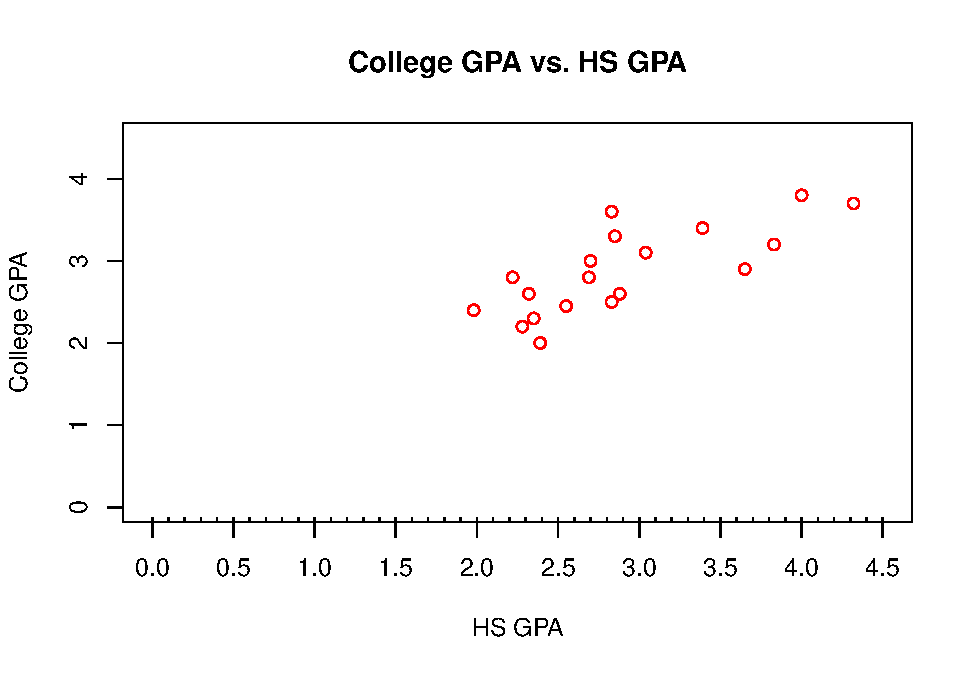
\includegraphics{01-Introduction-to-R_files/figure-latex/unnamed-chunk-40-1.pdf}

\begin{Shaded}
\begin{Highlighting}[]
 \FunctionTok{plot}\NormalTok{(}\AttributeTok{x =}\NormalTok{ gpacsv}\SpecialCharTok{$}\NormalTok{HSGPA, }\AttributeTok{y =}\NormalTok{ gpacsv}\SpecialCharTok{$}\NormalTok{CollegeGPA, }\AttributeTok{xlab =} \StringTok{"HS GPA"}\NormalTok{, }\AttributeTok{ylab =} \StringTok{"College GPA"}\NormalTok{,}
      \AttributeTok{main =} \FunctionTok{expression}\NormalTok{(}\FunctionTok{hat}\NormalTok{(Y) }\SpecialCharTok{==} \FunctionTok{hat}\NormalTok{(beta)[}\DecValTok{0}\NormalTok{] }\SpecialCharTok{+} \FunctionTok{hat}\NormalTok{(beta)[}\DecValTok{1}\NormalTok{]}\SpecialCharTok{*}\NormalTok{x),}
      \AttributeTok{xlim =} \FunctionTok{c}\NormalTok{(}\DecValTok{0}\NormalTok{,}\FloatTok{4.5}\NormalTok{), }\AttributeTok{ylim =} \FunctionTok{c}\NormalTok{(}\DecValTok{0}\NormalTok{,}\FloatTok{4.5}\NormalTok{), }\AttributeTok{col =} \StringTok{"red"}\NormalTok{, }\AttributeTok{pch =} \DecValTok{1}\NormalTok{, }\AttributeTok{cex =} \FloatTok{1.0}\NormalTok{, }\AttributeTok{panel.first=}\FunctionTok{grid}\NormalTok{(}\AttributeTok{col =} \StringTok{"gray"}\NormalTok{, }\AttributeTok{lty =} \StringTok{"dotted"}\NormalTok{))}

  \CommentTok{\#Draw a line from (x0, y0) to (x1, y1)}
  \FunctionTok{segments}\NormalTok{(}\AttributeTok{x0 =} \FunctionTok{min}\NormalTok{(gpacsv}\SpecialCharTok{$}\NormalTok{HSGPA), }\AttributeTok{y0 =}\NormalTok{ mod.fit}\SpecialCharTok{$}\NormalTok{coefficients[}\DecValTok{1}\NormalTok{] }\SpecialCharTok{+}\NormalTok{ mod.fit}\SpecialCharTok{$}\NormalTok{coefficients[}\DecValTok{2}\NormalTok{]}\SpecialCharTok{*}\FunctionTok{min}\NormalTok{(gpacsv}\SpecialCharTok{$}\NormalTok{HSGPA),}
           \AttributeTok{x1 =} \FunctionTok{max}\NormalTok{(gpacsv}\SpecialCharTok{$}\NormalTok{HSGPA), }\AttributeTok{y1 =}\NormalTok{ mod.fit}\SpecialCharTok{$}\NormalTok{coefficients[}\DecValTok{1}\NormalTok{] }\SpecialCharTok{+}\NormalTok{ mod.fit}\SpecialCharTok{$}\NormalTok{coefficients[}\DecValTok{2}\NormalTok{]}\SpecialCharTok{*}\FunctionTok{max}\NormalTok{(gpacsv}\SpecialCharTok{$}\NormalTok{HSGPA),}
           \AttributeTok{lty =} \DecValTok{1}\NormalTok{, }\AttributeTok{col =} \StringTok{"blue"}\NormalTok{, }\AttributeTok{lwd =} \DecValTok{2}\NormalTok{)}
\end{Highlighting}
\end{Shaded}

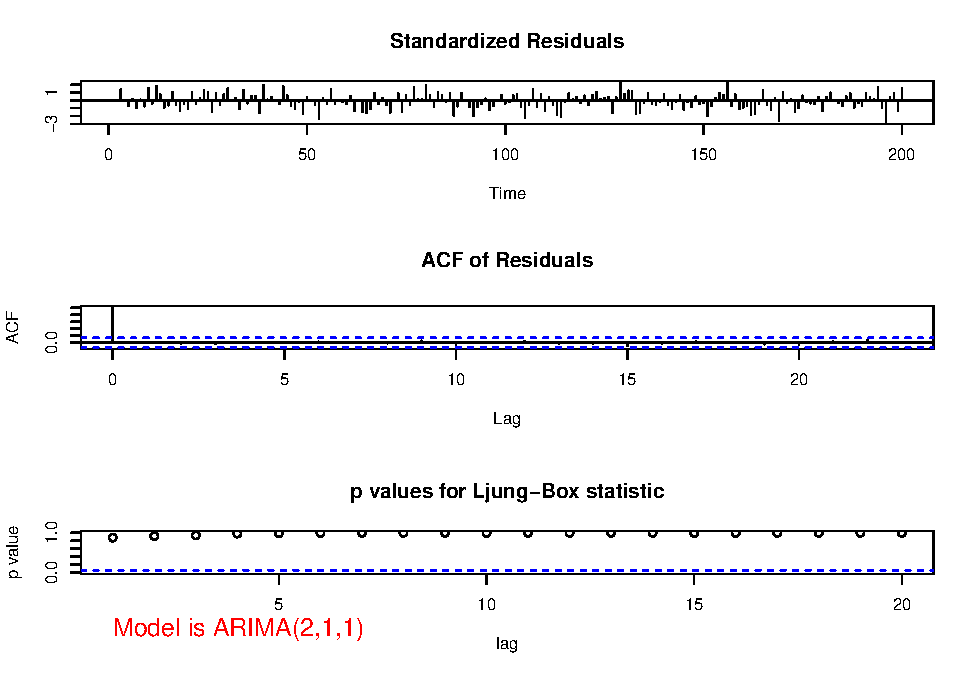
\includegraphics{01-Introduction-to-R_files/figure-latex/unnamed-chunk-41-1.pdf}

\begin{Shaded}
\begin{Highlighting}[]
  \FunctionTok{plot}\NormalTok{(}\AttributeTok{x =}\NormalTok{ gpacsv}\SpecialCharTok{$}\NormalTok{HSGPA, }\AttributeTok{y =}\NormalTok{ gpacsv}\SpecialCharTok{$}\NormalTok{CollegeGPA, }\AttributeTok{xlab =} \StringTok{"HS GPA"}\NormalTok{, }\AttributeTok{ylab =} \StringTok{"College GPA"}\NormalTok{,}
      \AttributeTok{main =} \FunctionTok{expression}\NormalTok{(}\FunctionTok{paste}\NormalTok{(}\StringTok{"College GPA vs. HS GPA and "}\NormalTok{, }\FunctionTok{widehat}\NormalTok{(CollegeGPA) }\SpecialCharTok{==} \FunctionTok{hat}\NormalTok{(beta)[}\DecValTok{0}\NormalTok{] }\SpecialCharTok{+} \FunctionTok{hat}\NormalTok{(beta)[}\DecValTok{1}\NormalTok{]}\SpecialCharTok{*}\NormalTok{HSGPA)),}
      \AttributeTok{xlim =} \FunctionTok{c}\NormalTok{(}\DecValTok{0}\NormalTok{,}\FloatTok{4.5}\NormalTok{), }\AttributeTok{ylim =} \FunctionTok{c}\NormalTok{(}\DecValTok{0}\NormalTok{,}\FloatTok{4.5}\NormalTok{), }\AttributeTok{col =} \StringTok{"red"}\NormalTok{, }\AttributeTok{pch =} \DecValTok{1}\NormalTok{, }\AttributeTok{cex =} \FloatTok{1.0}\NormalTok{, }\AttributeTok{panel.first=}\FunctionTok{grid}\NormalTok{(}\AttributeTok{col =} \StringTok{"gray"}\NormalTok{, }\AttributeTok{lty =} \StringTok{"dotted"}\NormalTok{))}
  
  \CommentTok{\#Draw a line from (x0, y0) to (x1, y1)}
  \FunctionTok{segments}\NormalTok{(}\AttributeTok{x0 =} \FunctionTok{min}\NormalTok{(gpacsv}\SpecialCharTok{$}\NormalTok{HSGPA), }\AttributeTok{y0 =}\NormalTok{ mod.fit}\SpecialCharTok{$}\NormalTok{coefficients[}\DecValTok{1}\NormalTok{] }\SpecialCharTok{+}\NormalTok{ mod.fit}\SpecialCharTok{$}\NormalTok{coefficients[}\DecValTok{2}\NormalTok{]}\SpecialCharTok{*}\FunctionTok{min}\NormalTok{(gpacsv}\SpecialCharTok{$}\NormalTok{HSGPA),}
           \AttributeTok{x1 =} \FunctionTok{max}\NormalTok{(gpacsv}\SpecialCharTok{$}\NormalTok{HSGPA), }\AttributeTok{y1 =}\NormalTok{ mod.fit}\SpecialCharTok{$}\NormalTok{coefficients[}\DecValTok{1}\NormalTok{] }\SpecialCharTok{+}\NormalTok{ mod.fit}\SpecialCharTok{$}\NormalTok{coefficients[}\DecValTok{2}\NormalTok{]}\SpecialCharTok{*}\FunctionTok{max}\NormalTok{(gpacsv}\SpecialCharTok{$}\NormalTok{HSGPA),}
           \AttributeTok{lty =} \DecValTok{1}\NormalTok{, }\AttributeTok{col =} \StringTok{"blue"}\NormalTok{, }\AttributeTok{lwd =} \DecValTok{2}\NormalTok{)}
\end{Highlighting}
\end{Shaded}

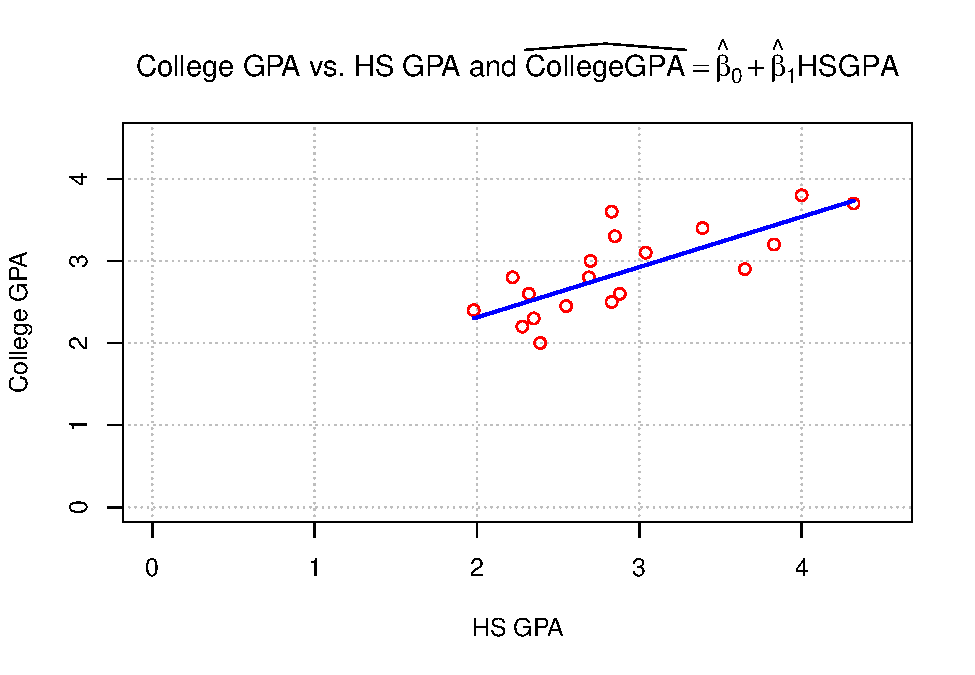
\includegraphics{01-Introduction-to-R_files/figure-latex/unnamed-chunk-41-2.pdf}

\begin{Shaded}
\begin{Highlighting}[]
\FunctionTok{demo}\NormalTok{(plotmath) }\CommentTok{\#Run this to see examples}
\end{Highlighting}
\end{Shaded}

\begin{verbatim}
## 
## 
##  demo(plotmath)
##  ---- ~~~~~~~~
## 
## > #  Copyright (C) 2002-2016 The R Core Team
## > 
## > require(datasets)
## 
## > require(grDevices); require(graphics)
## 
## > ## --- "math annotation" in plots :
## > 
## > ######
## > # create tables of mathematical annotation functionality
## > ######
## > make.table <- function(nr, nc) {
## +     savepar <- par(mar=rep(0, 4), pty="s")
## +     plot(c(0, nc*2 + 1), c(0, -(nr + 1)),
## +          type="n", xlab="", ylab="", axes=FALSE)
## +     savepar
## + }
## 
## > get.r <- function(i, nr) {
## +     i %% nr + 1
## + }
## 
## > get.c <- function(i, nr) {
## +     i %/% nr + 1
## + }
## 
## > draw.title.cell <- function(title, i, nr) {
## +     r <- get.r(i, nr)
## +     c <- get.c(i, nr)
## +     text(2*c - .5, -r, title)
## +     rect((2*(c - 1) + .5), -(r - .5), (2*c + .5), -(r + .5))
## + }
## 
## > draw.plotmath.cell <- function(expr, i, nr, string = NULL) {
## +     r <- get.r(i, nr)
## +     c <- get.c(i, nr)
## +     if (is.null(string)) {
## +         string <- deparse(expr)
## +         string <- substr(string, 12, nchar(string) - 1)
## +     }
## +     text((2*(c - 1) + 1), -r, string, col="grey50")
## +     text((2*c), -r, expr, adj=c(.5,.5))
## +     rect((2*(c - 1) + .5), -(r - .5), (2*c + .5), -(r + .5), border="grey")
## + }
## 
## > nr <- 20
## 
## > nc <- 2
## 
## > oldpar <- make.table(nr, nc)
\end{verbatim}

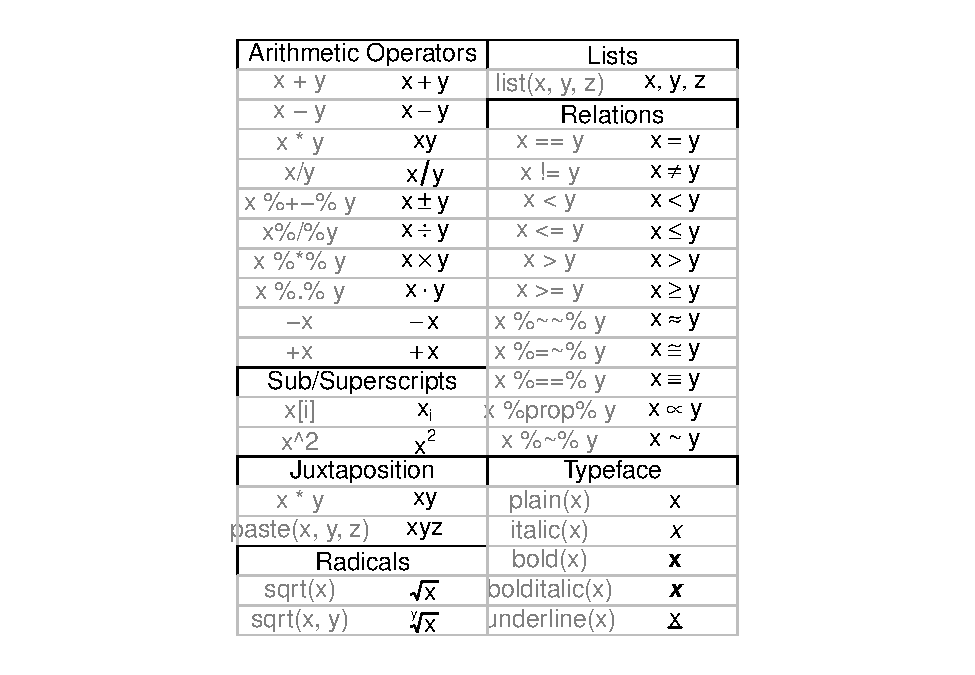
\includegraphics{01-Introduction-to-R_files/figure-latex/unnamed-chunk-42-1.pdf}

\begin{verbatim}
## 
## > i <- 0
## 
## > draw.title.cell("Arithmetic Operators", i, nr); i <- i + 1
## 
## > draw.plotmath.cell(expression(x + y), i, nr); i <- i + 1
## 
## > draw.plotmath.cell(expression(x - y), i, nr); i <- i + 1
## 
## > draw.plotmath.cell(expression(x * y), i, nr); i <- i + 1
## 
## > draw.plotmath.cell(expression(x / y), i, nr); i <- i + 1
## 
## > draw.plotmath.cell(expression(x %+-% y), i, nr); i <- i + 1
## 
## > draw.plotmath.cell(expression(x %/% y), i, nr); i <- i + 1
## 
## > draw.plotmath.cell(expression(x %*% y), i, nr); i <- i + 1
## 
## > draw.plotmath.cell(expression(x %.% y), i, nr); i <- i + 1
## 
## > draw.plotmath.cell(expression(-x), i, nr); i <- i + 1
## 
## > draw.plotmath.cell(expression(+x), i, nr); i <- i + 1
## 
## > draw.title.cell("Sub/Superscripts", i, nr); i <- i + 1
## 
## > draw.plotmath.cell(expression(x[i]), i, nr); i <- i + 1
## 
## > draw.plotmath.cell(expression(x^2), i, nr); i <- i + 1
## 
## > draw.title.cell("Juxtaposition", i, nr); i <- i + 1
## 
## > draw.plotmath.cell(expression(x * y), i, nr); i <- i + 1
## 
## > draw.plotmath.cell(expression(paste(x, y, z)), i, nr); i <- i + 1
## 
## > draw.title.cell("Radicals", i, nr); i <- i + 1
## 
## > draw.plotmath.cell(expression(sqrt(x)), i, nr); i <- i + 1
## 
## > draw.plotmath.cell(expression(sqrt(x, y)), i, nr); i <- i + 1
## 
## > draw.title.cell("Lists", i, nr); i <- i + 1
## 
## > draw.plotmath.cell(expression(list(x, y, z)), i, nr); i <- i + 1
## 
## > draw.title.cell("Relations", i, nr); i <- i + 1
## 
## > draw.plotmath.cell(expression(x == y), i, nr); i <- i + 1
## 
## > draw.plotmath.cell(expression(x != y), i, nr); i <- i + 1
## 
## > draw.plotmath.cell(expression(x < y), i, nr); i <- i + 1
## 
## > draw.plotmath.cell(expression(x <= y), i, nr); i <- i + 1
## 
## > draw.plotmath.cell(expression(x > y), i, nr); i <- i + 1
## 
## > draw.plotmath.cell(expression(x >= y), i, nr); i <- i + 1
## 
## > draw.plotmath.cell(expression(x %~~% y), i, nr); i <- i + 1
## 
## > draw.plotmath.cell(expression(x %=~% y), i, nr); i <- i + 1
## 
## > draw.plotmath.cell(expression(x %==% y), i, nr); i <- i + 1
## 
## > draw.plotmath.cell(expression(x %prop% y), i, nr); i <- i + 1
## 
## > draw.plotmath.cell(expression(x %~% y), i, nr); i <- i + 1
## 
## > draw.title.cell("Typeface", i, nr); i <- i + 1
## 
## > draw.plotmath.cell(expression(plain(x)), i, nr); i <- i + 1
## 
## > draw.plotmath.cell(expression(italic(x)), i, nr); i <- i + 1
## 
## > draw.plotmath.cell(expression(bold(x)), i, nr); i <- i + 1
## 
## > draw.plotmath.cell(expression(bolditalic(x)), i, nr); i <- i + 1
## 
## > draw.plotmath.cell(expression(underline(x)), i, nr); i <- i + 1
## 
## > # Need fewer, wider columns for ellipsis ...
## > nr <- 20
## 
## > nc <- 2
## 
## > make.table(nr, nc)
\end{verbatim}

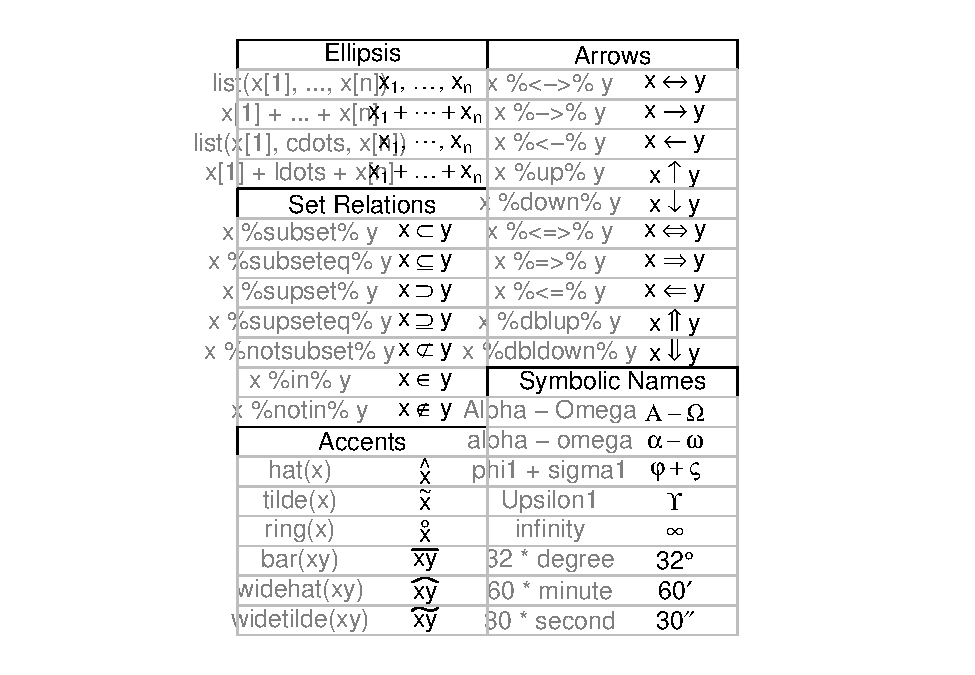
\includegraphics{01-Introduction-to-R_files/figure-latex/unnamed-chunk-42-2.pdf}

\begin{verbatim}
## $mar
## [1] 0 0 0 0
## 
## $pty
## [1] "s"
## 
## 
## > i <- 0
## 
## > draw.title.cell("Ellipsis", i, nr); i <- i + 1
## 
## > draw.plotmath.cell(expression(list(x[1], ..., x[n])), i, nr); i <- i + 1
## 
## > draw.plotmath.cell(expression(x[1] + ... + x[n]), i, nr); i <- i + 1
## 
## > draw.plotmath.cell(expression(list(x[1], cdots, x[n])), i, nr); i <- i + 1
## 
## > draw.plotmath.cell(expression(x[1] + ldots + x[n]), i, nr); i <- i + 1
## 
## > draw.title.cell("Set Relations", i, nr); i <- i + 1
## 
## > draw.plotmath.cell(expression(x %subset% y), i, nr); i <- i + 1
## 
## > draw.plotmath.cell(expression(x %subseteq% y), i, nr); i <- i + 1
## 
## > draw.plotmath.cell(expression(x %supset% y), i, nr); i <- i + 1
## 
## > draw.plotmath.cell(expression(x %supseteq% y), i, nr); i <- i + 1
## 
## > draw.plotmath.cell(expression(x %notsubset% y), i, nr); i <- i + 1
## 
## > draw.plotmath.cell(expression(x %in% y), i, nr); i <- i + 1
## 
## > draw.plotmath.cell(expression(x %notin% y), i, nr); i <- i + 1
## 
## > draw.title.cell("Accents", i, nr); i <- i + 1
## 
## > draw.plotmath.cell(expression(hat(x)), i, nr); i <- i + 1
## 
## > draw.plotmath.cell(expression(tilde(x)), i, nr); i <- i + 1
## 
## > draw.plotmath.cell(expression(ring(x)), i, nr); i <- i + 1
## 
## > draw.plotmath.cell(expression(bar(xy)), i, nr); i <- i + 1
## 
## > draw.plotmath.cell(expression(widehat(xy)), i, nr); i <- i + 1
## 
## > draw.plotmath.cell(expression(widetilde(xy)), i, nr); i <- i + 1
## 
## > draw.title.cell("Arrows", i, nr); i <- i + 1
## 
## > draw.plotmath.cell(expression(x %<->% y), i, nr); i <- i + 1
## 
## > draw.plotmath.cell(expression(x %->% y), i, nr); i <- i + 1
## 
## > draw.plotmath.cell(expression(x %<-% y), i, nr); i <- i + 1
## 
## > draw.plotmath.cell(expression(x %up% y), i, nr); i <- i + 1
## 
## > draw.plotmath.cell(expression(x %down% y), i, nr); i <- i + 1
## 
## > draw.plotmath.cell(expression(x %<=>% y), i, nr); i <- i + 1
## 
## > draw.plotmath.cell(expression(x %=>% y), i, nr); i <- i + 1
## 
## > draw.plotmath.cell(expression(x %<=% y), i, nr); i <- i + 1
## 
## > draw.plotmath.cell(expression(x %dblup% y), i, nr); i <- i + 1
## 
## > draw.plotmath.cell(expression(x %dbldown% y), i, nr); i <- i + 1
## 
## > draw.title.cell("Symbolic Names", i, nr); i <- i + 1
## 
## > draw.plotmath.cell(expression(Alpha - Omega), i, nr); i <- i + 1
## 
## > draw.plotmath.cell(expression(alpha - omega), i, nr); i <- i + 1
## 
## > draw.plotmath.cell(expression(phi1 + sigma1), i, nr); i <- i + 1
## 
## > draw.plotmath.cell(expression(Upsilon1), i, nr); i <- i + 1
## 
## > draw.plotmath.cell(expression(infinity), i, nr); i <- i + 1
## 
## > draw.plotmath.cell(expression(32 * degree), i, nr); i <- i + 1
## 
## > draw.plotmath.cell(expression(60 * minute), i, nr); i <- i + 1
## 
## > draw.plotmath.cell(expression(30 * second), i, nr); i <- i + 1
## 
## > # Need even fewer, wider columns for typeface and style ...
## > nr <- 20
## 
## > nc <- 1
## 
## > make.table(nr, nc)
\end{verbatim}

\begin{verbatim}
## $mar
## [1] 0 0 0 0
## 
## $pty
## [1] "s"
## 
## 
## > i <- 0
## 
## > draw.title.cell("Style", i, nr); i <- i + 1
## 
## > draw.plotmath.cell(expression(displaystyle(x)), i, nr); i <- i + 1
## 
## > draw.plotmath.cell(expression(textstyle(x)), i, nr); i <- i + 1
## 
## > draw.plotmath.cell(expression(scriptstyle(x)), i, nr); i <- i + 1
## 
## > draw.plotmath.cell(expression(scriptscriptstyle(x)), i, nr); i <- i + 1
## 
## > draw.title.cell("Spacing", i, nr); i <- i + 1
## 
## > draw.plotmath.cell(expression(x ~~ y), i, nr); i <- i + 1
## 
## > # Need fewer, taller rows for fractions ...
## > # cheat a bit to save pages
## > par(new = TRUE)
## 
## > nr <- 10
## 
## > nc <- 1
## 
## > make.table(nr, nc)
\end{verbatim}

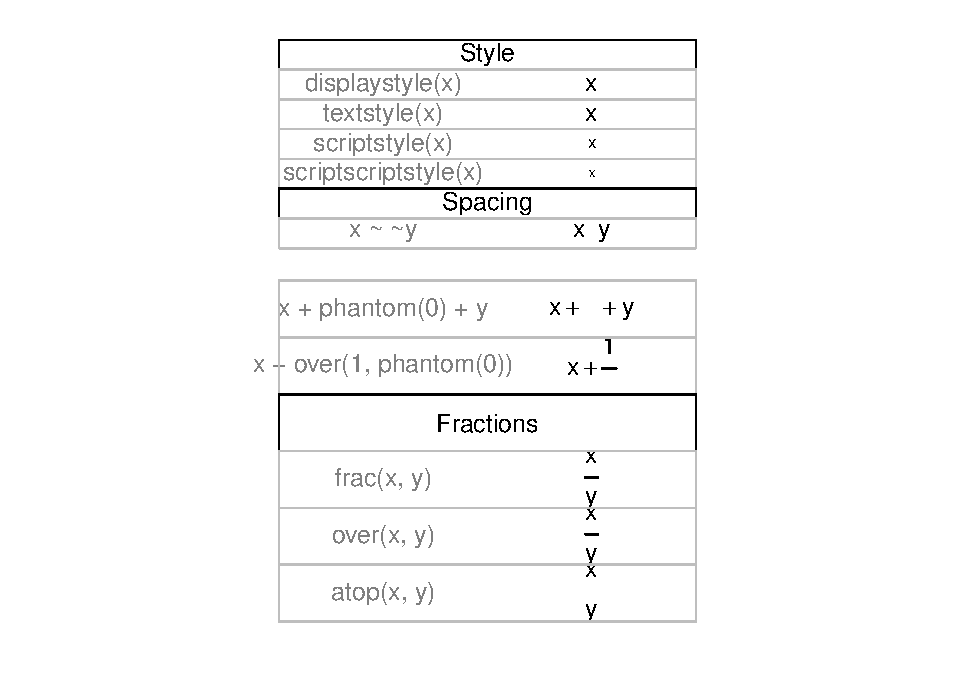
\includegraphics{01-Introduction-to-R_files/figure-latex/unnamed-chunk-42-3.pdf}

\begin{verbatim}
## $mar
## [1] 0 0 0 0
## 
## $pty
## [1] "s"
## 
## 
## > i <- 4
## 
## > draw.plotmath.cell(expression(x + phantom(0) + y), i, nr); i <- i + 1
## 
## > draw.plotmath.cell(expression(x + over(1, phantom(0))), i, nr); i <- i + 1
## 
## > draw.title.cell("Fractions", i, nr); i <- i + 1
## 
## > draw.plotmath.cell(expression(frac(x, y)), i, nr); i <- i + 1
## 
## > draw.plotmath.cell(expression(over(x, y)), i, nr); i <- i + 1
## 
## > draw.plotmath.cell(expression(atop(x, y)), i, nr); i <- i + 1
## 
## > # Need fewer, taller rows and fewer, wider columns for big operators ...
## > nr <- 10
## 
## > nc <- 1
## 
## > make.table(nr, nc)
\end{verbatim}

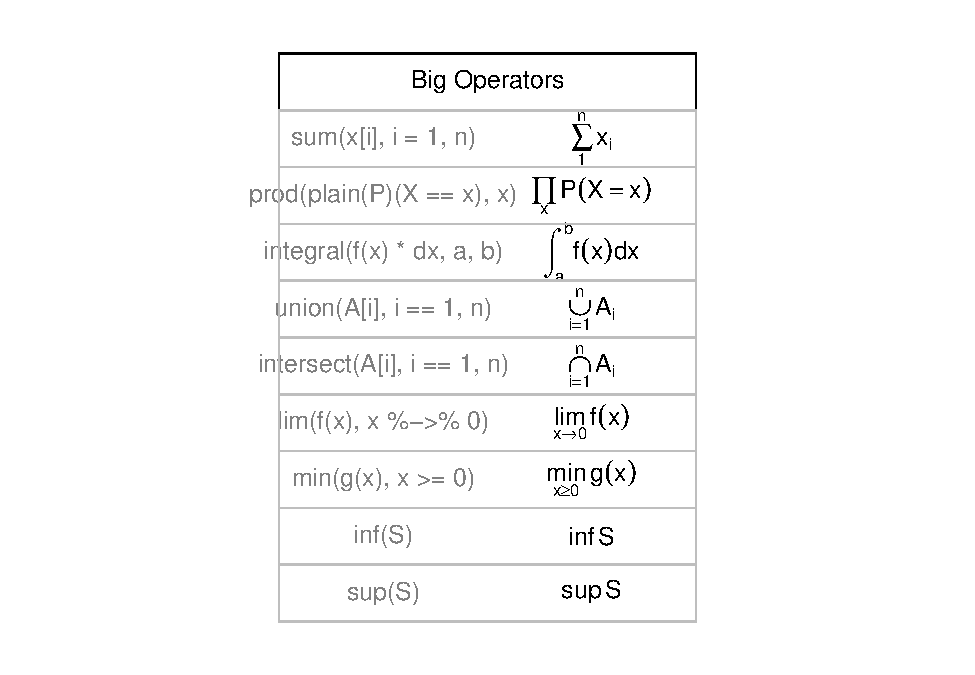
\includegraphics{01-Introduction-to-R_files/figure-latex/unnamed-chunk-42-4.pdf}

\begin{verbatim}
## $mar
## [1] 0 0 0 0
## 
## $pty
## [1] "s"
## 
## 
## > i <- 0
## 
## > draw.title.cell("Big Operators", i, nr); i <- i + 1
## 
## > draw.plotmath.cell(expression(sum(x[i], i=1, n)), i, nr); i <- i + 1
## 
## > draw.plotmath.cell(expression(prod(plain(P)(X == x), x)), i, nr); i <- i + 1
## 
## > draw.plotmath.cell(expression(integral(f(x) * dx, a, b)), i, nr); i <- i + 1
## 
## > draw.plotmath.cell(expression(union(A[i], i==1, n)), i, nr); i <- i + 1
## 
## > draw.plotmath.cell(expression(intersect(A[i], i==1, n)), i, nr); i <- i + 1
## 
## > draw.plotmath.cell(expression(lim(f(x), x %->% 0)), i, nr); i <- i + 1
## 
## > draw.plotmath.cell(expression(min(g(x), x >= 0)), i, nr); i <- i + 1
## 
## > draw.plotmath.cell(expression(inf(S)), i, nr); i <- i + 1
## 
## > draw.plotmath.cell(expression(sup(S)), i, nr); i <- i + 1
## 
## > nr <- 12
## 
## > nc <- 1
## 
## > make.table(nr, nc)
\end{verbatim}

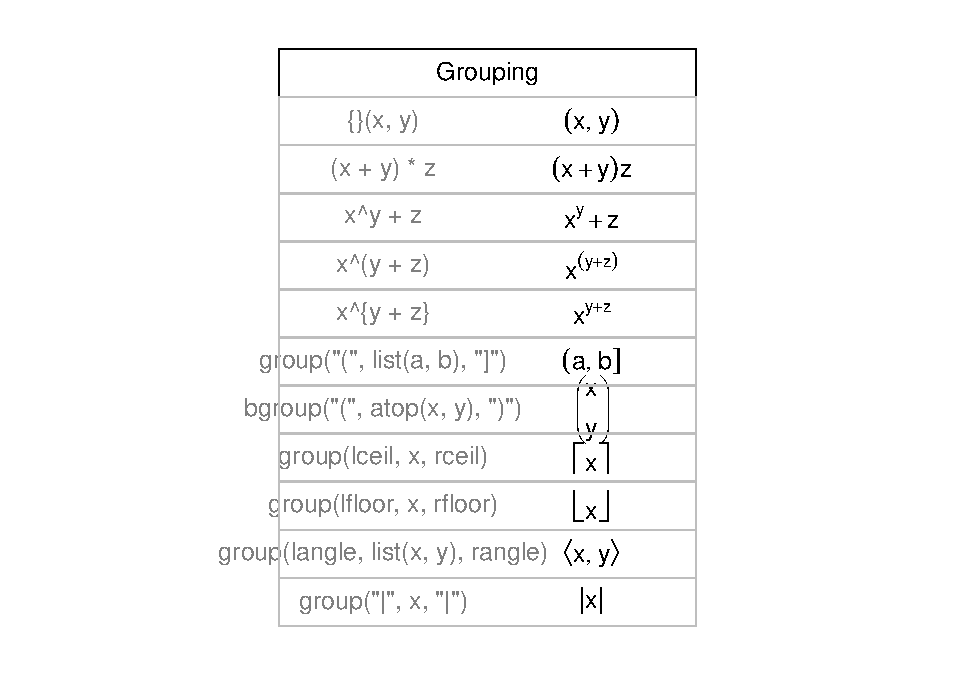
\includegraphics{01-Introduction-to-R_files/figure-latex/unnamed-chunk-42-5.pdf}

\begin{verbatim}
## $mar
## [1] 0 0 0 0
## 
## $pty
## [1] "s"
## 
## 
## > i <- 0
## 
## > draw.title.cell("Grouping", i, nr); i <- i + 1
## 
## > # Those involving '{ . }' have to be done "by hand"
## > draw.plotmath.cell(expression({}(x , y)), i, nr, string="{}(x, y)"); i <- i + 1
## 
## > draw.plotmath.cell(expression((x + y)*z), i, nr); i <- i + 1
## 
## > draw.plotmath.cell(expression(x^y + z),   i, nr); i <- i + 1
## 
## > draw.plotmath.cell(expression(x^(y + z)), i, nr); i <- i + 1
## 
## > draw.plotmath.cell(expression(x^{y + z}), i, nr, string="x^{y + z}"); i <- i + 1
## 
## > draw.plotmath.cell(expression(group("(", list(a, b), "]")), i, nr); i <- i + 1
## 
## > draw.plotmath.cell(expression(bgroup("(", atop(x, y), ")")), i, nr); i <- i + 1
## 
## > draw.plotmath.cell(expression(group(lceil, x, rceil)), i, nr); i <- i + 1
## 
## > draw.plotmath.cell(expression(group(lfloor, x, rfloor)), i, nr); i <- i + 1
## 
## > draw.plotmath.cell(expression(group(langle, list(x, y), rangle)), i, nr); i <- i + 1
## 
## > draw.plotmath.cell(expression(group("|", x, "|")), i, nr); i <- i + 1
## 
## > par(oldpar)
\end{verbatim}

\hypertarget{object-oriented-language}{%
\section{Object-Oriented Language}\label{object-oriented-language}}

Functions are typically designed to operate on only one or very few classes of objects. However, some functions, like \texttt{summary()}, are \textbf{generic}, in the sense that essentially different versions of them have been constructed to work with different classes of objects.

When a generic function is run with an object, R first checks the object's class type and then looks to find a method function with the name format \texttt{\textless{}generic\ function\textgreater{}.\textless{}class\ name\textgreater{}}. Below are examples for \texttt{summary()}:

\begin{itemize}
\tightlist
\item
  summary(mod.fit) -- The function \texttt{summary.lm()} summarizes the regression model
\item
  summary(gpacsv) -- The function \texttt{summary.data.frame()} summarizes the data frame's contents
\item
  summary.default() -- R attempts to run this function if there is no method function for a class
\end{itemize}

There are many generic functions! For example, \texttt{plot()} is a generic function (try\texttt{plot(mod.fit)} to see what happens!). We will also see other generic functions like \texttt{predict()} later in the notes.

\begin{Shaded}
\begin{Highlighting}[]
\FunctionTok{plot}\NormalTok{(mod.fit)}
\end{Highlighting}
\end{Shaded}

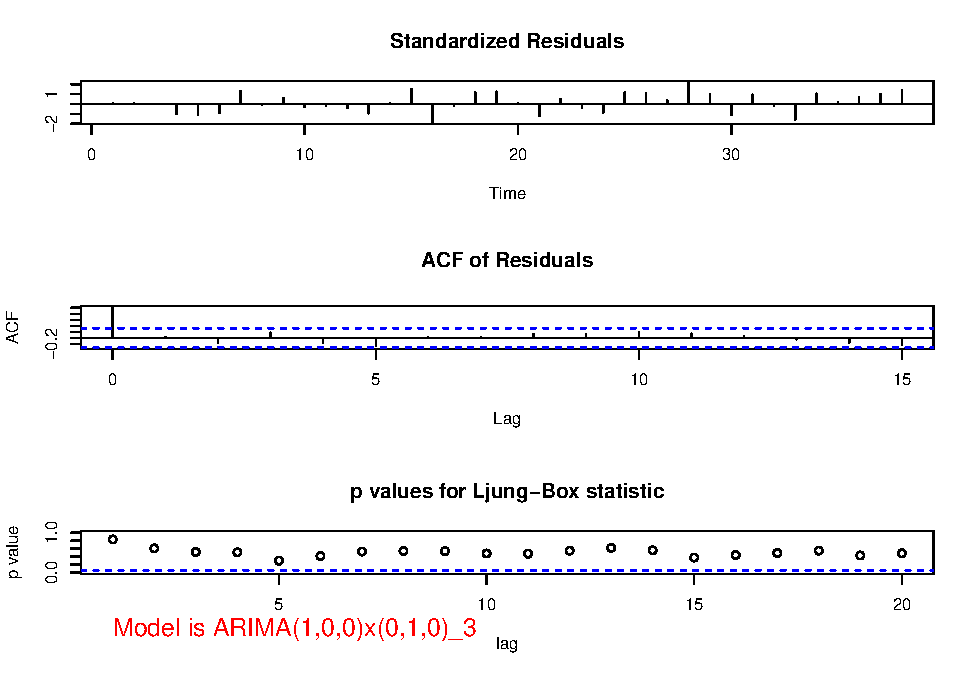
\includegraphics{01-Introduction-to-R_files/figure-latex/unnamed-chunk-43-1.pdf} 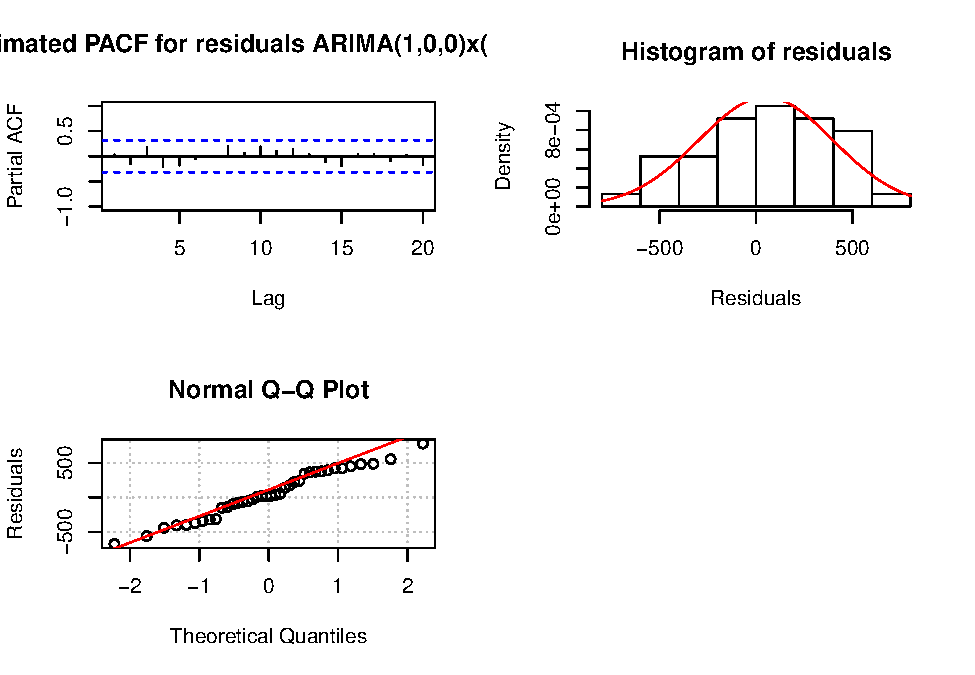
\includegraphics{01-Introduction-to-R_files/figure-latex/unnamed-chunk-43-2.pdf} 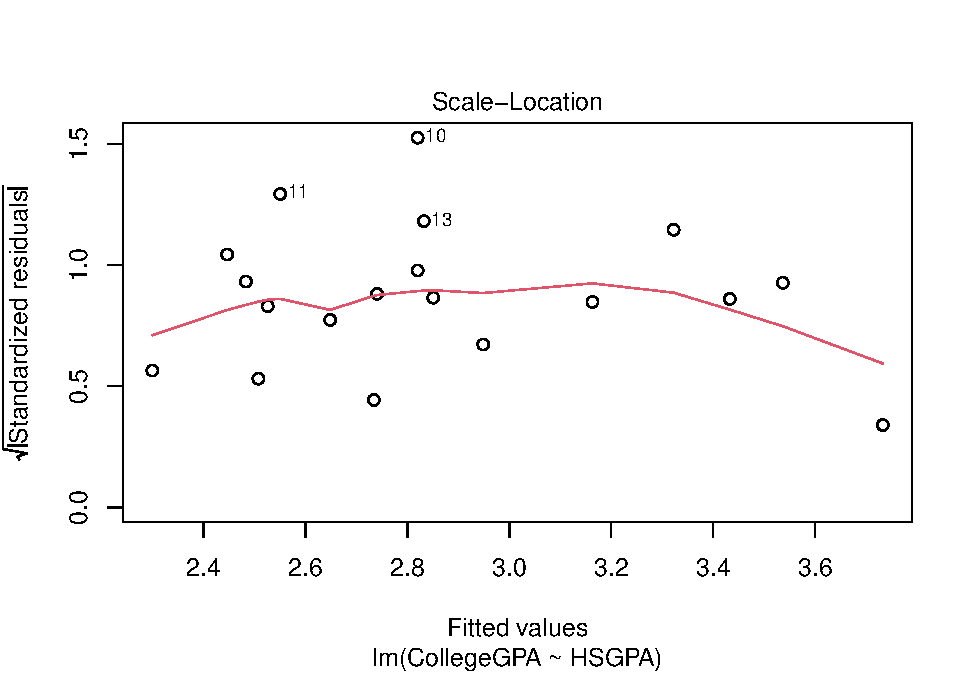
\includegraphics{01-Introduction-to-R_files/figure-latex/unnamed-chunk-43-3.pdf} 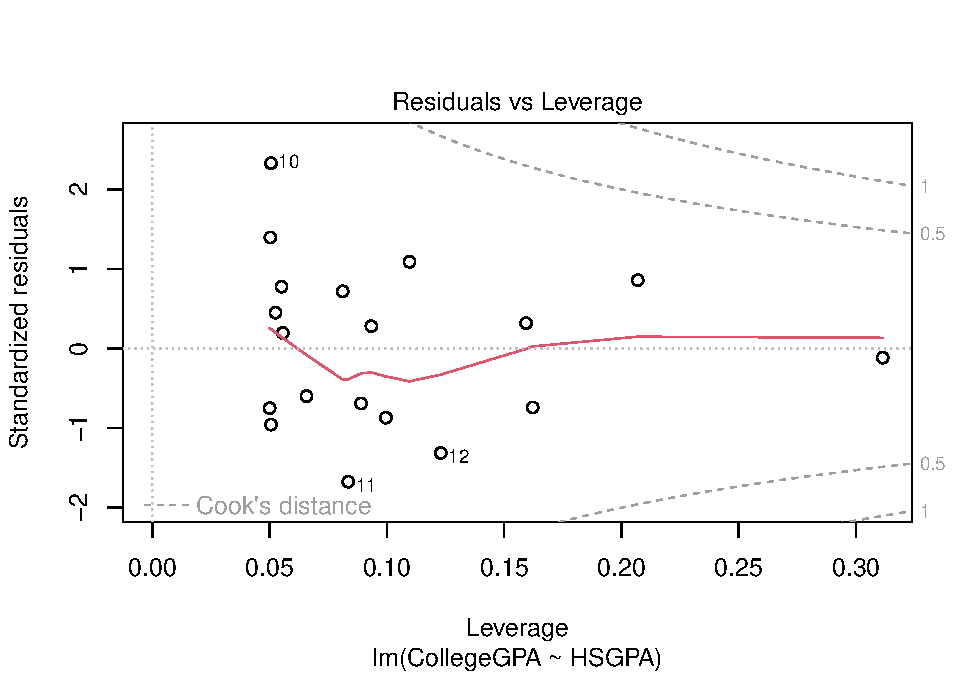
\includegraphics{01-Introduction-to-R_files/figure-latex/unnamed-chunk-43-4.pdf}

The purpose of generic functions is to use a familiar language set with any object. So it is convenient to use the same language set no matter the application. This is why R is referred to as an object-oriented language.

To see a list of all method functions associated with a class, use \texttt{methods(class\ =\ \textless{}class\ name\textgreater{})}. For the regression example, the method functions associated with the \texttt{lm} class are:

\begin{Shaded}
\begin{Highlighting}[]
\FunctionTok{methods}\NormalTok{(}\AttributeTok{class=}\StringTok{"lm"}\NormalTok{) }\SpecialCharTok{\%\textgreater{}\%} \FunctionTok{head}\NormalTok{()}
\end{Highlighting}
\end{Shaded}

\begin{verbatim}
## [1] "add1.lm"                   "alias.lm"                 
## [3] "anova.lm"                  "case.names.lm"            
## [5] "coerce,oldClass,S3-method" "confint.lm"
\end{verbatim}

To see a list of all method functions for a generic function, use \texttt{methods(generic.function\ =\ \textless{}generic\ function\ name\textgreater{})}

\begin{Shaded}
\begin{Highlighting}[]
\FunctionTok{methods}\NormalTok{(}\AttributeTok{generic.function =} \StringTok{"summary"}\NormalTok{) }\SpecialCharTok{\%\textgreater{}\%} \FunctionTok{head}\NormalTok{()}
\end{Highlighting}
\end{Shaded}

\begin{verbatim}
## [1] "summary.aov"                   "summary.aovlist"              
## [3] "summary.aspell"                "summary.check_packages_in_dir"
## [5] "summary.connection"            "summary.data.frame"
\end{verbatim}

Knowing what a name of a particular method function can be helpful to find help on it. For example, the help for \texttt{summary()} alone is not very helpful! However, the help for \texttt{summary.lm()}provides a lot of useful information about what is summarized for a regression model.

\hypertarget{plotting}{%
\chapter{Plotting}\label{plotting}}

In this chapter, we will go over some \emph{Time Series} examples.
The aim of this chapter is to help you grasp some of the ideas about plotting.

\hypertarget{example-data}{%
\section{Example Data}\label{example-data}}

Click \href{http://www.chrisbilder.com/stat878/sections/2/OSU_enroll.csv}{OSU\_enroll.csv} to download data.

\begin{Shaded}
\begin{Highlighting}[]
\NormalTok{osu.enroll }\OtherTok{\textless{}{-}} \FunctionTok{read.csv}\NormalTok{(}\AttributeTok{file =} \StringTok{"OSU\_enroll.csv"}\NormalTok{, }
    \AttributeTok{stringsAsFactors =} \ConstantTok{TRUE}\NormalTok{)}
\end{Highlighting}
\end{Shaded}

\begin{Shaded}
\begin{Highlighting}[]
\FunctionTok{head}\NormalTok{(osu.enroll)}
\end{Highlighting}
\end{Shaded}

\begin{verbatim}
##   t Semester Year Enrollment      date
## 1 1     Fall 1989      20110 8/31/1989
## 2 2   Spring 1990      19128  2/1/1990
## 3 3   Summer 1990       7553  6/1/1990
## 4 4     Fall 1990      19591 8/31/1990
## 5 5   Spring 1991      18361  2/1/1991
## 6 6   Summer 1991       6702  6/1/1991
\end{verbatim}

\begin{Shaded}
\begin{Highlighting}[]
\FunctionTok{tail}\NormalTok{(osu.enroll)}
\end{Highlighting}
\end{Shaded}

\begin{verbatim}
##     t Semester Year Enrollment      date
## 35 35   Spring 2001      20004  2/1/2001
## 36 36   Summer 2001       7558  6/1/2001
## 37 37     Fall 2001      21872 8/31/2001
## 38 38   Spring 2002      20922  2/1/2002
## 39 39   Summer 2002       7868  6/1/2002
## 40 40     Fall 2002      22992 8/31/2002
\end{verbatim}

\begin{Shaded}
\begin{Highlighting}[]
\NormalTok{x }\OtherTok{\textless{}{-}}\NormalTok{ osu.enroll}\SpecialCharTok{$}\NormalTok{Enrollment}
\end{Highlighting}
\end{Shaded}

\begin{Shaded}
\begin{Highlighting}[]
\CommentTok{\#One way to do plot}
\FunctionTok{dev.new}\NormalTok{(}\AttributeTok{width =} \DecValTok{8}\NormalTok{, }\AttributeTok{height =} \DecValTok{6}\NormalTok{, }\AttributeTok{pointsize =} \DecValTok{10}\NormalTok{) }

\CommentTok{\# we did not specify y{-}axis and R put our x in y{-}axis, time in  x{-}axis}

\FunctionTok{plot}\NormalTok{(}\AttributeTok{x =}\NormalTok{ x, }\AttributeTok{ylab =} \StringTok{"OSU Enrollment"}\NormalTok{, }
       \AttributeTok{xlab =} \StringTok{"t (time)"}\NormalTok{, }\AttributeTok{type=}\StringTok{"l"}\NormalTok{, }\AttributeTok{col =} \StringTok{"red"}\NormalTok{, }
       \AttributeTok{main =} \StringTok{"OSU Enrollment from Fall 1989 to Fall 2002"}\NormalTok{, }
       \AttributeTok{panel.first =} \FunctionTok{grid}\NormalTok{(}\AttributeTok{col =} \StringTok{"gray"}\NormalTok{, }\AttributeTok{lty =} \StringTok{"dotted"}\NormalTok{))}
\FunctionTok{points}\NormalTok{(}\AttributeTok{x =}\NormalTok{ x, }\AttributeTok{pch =} \DecValTok{20}\NormalTok{, }\AttributeTok{col =} \StringTok{"blue"}\NormalTok{)}
\end{Highlighting}
\end{Shaded}

\begin{Shaded}
\begin{Highlighting}[]
\CommentTok{\# A little different version of the plot}
  \FunctionTok{plot}\NormalTok{(}\AttributeTok{x =}\NormalTok{ x, }\AttributeTok{ylab =} \StringTok{"OSU Enrollment"}\NormalTok{, }\AttributeTok{type =} \StringTok{"o"}\NormalTok{, }\AttributeTok{xlab =} \StringTok{"t (time)"}\NormalTok{, }\AttributeTok{col =} \StringTok{"red"}\NormalTok{,}
    \AttributeTok{main =} \StringTok{"OSU enrollment data"}\NormalTok{, }\AttributeTok{panel.first =} \FunctionTok{grid}\NormalTok{(}\AttributeTok{col =} \StringTok{"gray"}\NormalTok{, }\AttributeTok{lty =} \StringTok{"dotted"}\NormalTok{))}
\end{Highlighting}
\end{Shaded}

\includegraphics{02-Plotting_files/figure-latex/unnamed-chunk-6-1.pdf}

\begin{Shaded}
\begin{Highlighting}[]
\FunctionTok{dev.new}\NormalTok{(}\AttributeTok{width =} \DecValTok{8}\NormalTok{, }\AttributeTok{height =} \DecValTok{6}\NormalTok{, }\AttributeTok{pointsize =} \DecValTok{10}\NormalTok{) }

\CommentTok{\# we did not specify y{-}axis and R put our x in y{-}axis, time in  x{-}axis}

\FunctionTok{plot}\NormalTok{(}\AttributeTok{x =}\NormalTok{ x, }\AttributeTok{ylab =} \StringTok{"OSU Enrollment"}\NormalTok{, }
       \AttributeTok{xlab =} \StringTok{"t (time)"}\NormalTok{, }\AttributeTok{type=}\StringTok{"l"}\NormalTok{, }\AttributeTok{col =} \StringTok{"red"}\NormalTok{, }
       \AttributeTok{main =} \StringTok{"OSU Enrollment from Fall 1989 to Fall 2002"}\NormalTok{, }
       \AttributeTok{panel.first =} \FunctionTok{grid}\NormalTok{(}\AttributeTok{col =} \StringTok{"gray"}\NormalTok{, }\AttributeTok{lty =} \StringTok{"dotted"}\NormalTok{))}

\FunctionTok{points}\NormalTok{(}\AttributeTok{x =}\NormalTok{ osu.enroll}\SpecialCharTok{$}\NormalTok{Enrollment, }\AttributeTok{pch =} \DecValTok{20}\NormalTok{, }\AttributeTok{col =} \StringTok{"blue"}\NormalTok{)}
\end{Highlighting}
\end{Shaded}

Altenatively, you can do the same thing using ggplot.

\begin{Shaded}
\begin{Highlighting}[]
\FunctionTok{library}\NormalTok{(ggplot2)}

\CommentTok{\# Create a data frame}
\NormalTok{df }\OtherTok{\textless{}{-}} \FunctionTok{data.frame}\NormalTok{(osu.enroll)}

\CommentTok{\# Create the plot}
\FunctionTok{ggplot}\NormalTok{(df, }\FunctionTok{aes}\NormalTok{(}\AttributeTok{x =}\NormalTok{ t, }\AttributeTok{y =}\NormalTok{ Enrollment)) }\SpecialCharTok{+}
  \FunctionTok{geom\_line}\NormalTok{(}\AttributeTok{colour =} \StringTok{"red"}\NormalTok{) }\SpecialCharTok{+}  \CommentTok{\# Line plot}
  \FunctionTok{geom\_point}\NormalTok{(}\AttributeTok{shape =} \DecValTok{20}\NormalTok{, }\AttributeTok{colour =} \StringTok{"blue"}\NormalTok{) }\SpecialCharTok{+}  \CommentTok{\# Add points}
  \FunctionTok{labs}\NormalTok{(}\AttributeTok{x =} \StringTok{"t (time)"}\NormalTok{, }\AttributeTok{y =} \StringTok{"OSU Enrollment"}\NormalTok{, }
       \AttributeTok{title =} \StringTok{"OSU Enrollment from Fall 1989 to Fall 2002"}\NormalTok{) }\SpecialCharTok{+}  \CommentTok{\# Set axis labels and title}
  \FunctionTok{theme\_bw}\NormalTok{() }\SpecialCharTok{+}  \CommentTok{\# Set the theme to a white background with black lines}
  \FunctionTok{theme}\NormalTok{(}\AttributeTok{panel.grid.major =} \FunctionTok{element\_line}\NormalTok{(}\AttributeTok{colour =} \StringTok{"gray"}\NormalTok{, }\AttributeTok{linetype =} \StringTok{"dotted"}\NormalTok{))  }\CommentTok{\# Add gray dotted lines to the plot}
\end{Highlighting}
\end{Shaded}

\includegraphics{02-Plotting_files/figure-latex/unnamed-chunk-8-1.pdf}

When only x is specified in the \texttt{plot()} function, R puts this on the y-axis and uses the observation number on the x-axis.

Compare this to the next plot below where both x and y arguments are specified.

\begin{Shaded}
\begin{Highlighting}[]
\CommentTok{\#More complicated plot}
\NormalTok{fall }\OtherTok{\textless{}{-}}\NormalTok{ osu.enroll[osu.enroll}\SpecialCharTok{$}\NormalTok{Semester }\SpecialCharTok{==} \StringTok{"Fall"}\NormalTok{,]}
\NormalTok{spring }\OtherTok{\textless{}{-}}\NormalTok{ osu.enroll[osu.enroll}\SpecialCharTok{$}\NormalTok{Semester }\SpecialCharTok{==} \StringTok{"Spring"}\NormalTok{,]}
\NormalTok{summer }\OtherTok{\textless{}{-}}\NormalTok{ osu.enroll[osu.enroll}\SpecialCharTok{$}\NormalTok{Semester }\SpecialCharTok{==} \StringTok{"Summer"}\NormalTok{,]}

\FunctionTok{plot}\NormalTok{(}\AttributeTok{y =}\NormalTok{ fall}\SpecialCharTok{$}\NormalTok{Enrollment, }\AttributeTok{x =}\NormalTok{ fall}\SpecialCharTok{$}\NormalTok{t,}
    \AttributeTok{ylab =} \StringTok{"OSU Enrollment"}\NormalTok{, }\AttributeTok{xlab =} \StringTok{"t (time)"}\NormalTok{, }
    \AttributeTok{col =} \StringTok{"blue"}\NormalTok{, }
    \AttributeTok{main =} \StringTok{"OSU Enrollment from Fall 1989 to Fall 2002"}\NormalTok{, }
    \AttributeTok{panel.first =} \FunctionTok{grid}\NormalTok{(}\AttributeTok{col =} \StringTok{"gray"}\NormalTok{, }\AttributeTok{lty =} \StringTok{"dotted"}\NormalTok{), }
    \AttributeTok{pch =} \DecValTok{1}\NormalTok{, }\AttributeTok{type =} \StringTok{"o"}\NormalTok{, }\AttributeTok{ylim =} \FunctionTok{c}\NormalTok{(}\DecValTok{0}\NormalTok{,}\FunctionTok{max}\NormalTok{(osu.enroll}\SpecialCharTok{$}\NormalTok{Enrollment)))}

\FunctionTok{lines}\NormalTok{(}\AttributeTok{y =}\NormalTok{ spring}\SpecialCharTok{$}\NormalTok{Enrollment, }\AttributeTok{x =}\NormalTok{ spring}\SpecialCharTok{$}\NormalTok{t, }\AttributeTok{col =} \StringTok{"red"}\NormalTok{, }
    \AttributeTok{type =} \StringTok{"o"}\NormalTok{, }\AttributeTok{pch =} \DecValTok{2}\NormalTok{)}

\FunctionTok{lines}\NormalTok{(}\AttributeTok{y =}\NormalTok{ summer}\SpecialCharTok{$}\NormalTok{Enrollment, }\AttributeTok{x =}\NormalTok{ summer}\SpecialCharTok{$}\NormalTok{t, }\AttributeTok{col =} 
    \StringTok{"darkgreen"}\NormalTok{, }\AttributeTok{type =} \StringTok{"o"}\NormalTok{, }\AttributeTok{pch =} \DecValTok{3}\NormalTok{)}
    
\FunctionTok{legend}\NormalTok{(}\AttributeTok{x=}\StringTok{"center"}\NormalTok{, }\AttributeTok{legend=} \FunctionTok{c}\NormalTok{(}\StringTok{"Fall"}\NormalTok{,}\StringTok{"Spring"}\NormalTok{,}\StringTok{"Summer"}\NormalTok{), }\AttributeTok{pch=}\FunctionTok{c}\NormalTok{(}\DecValTok{1}\NormalTok{,}\DecValTok{2}\NormalTok{,}\DecValTok{3}\NormalTok{), }\AttributeTok{lty=}\FunctionTok{c}\NormalTok{(}\DecValTok{1}\NormalTok{,}\DecValTok{1}\NormalTok{,}\DecValTok{1}\NormalTok{), }\AttributeTok{col=}\FunctionTok{c}\NormalTok{(}\StringTok{"blue"}\NormalTok{,}\StringTok{"red"}\NormalTok{,}\StringTok{"darkgreen"}\NormalTok{), }\AttributeTok{bty=}\StringTok{"n"}\NormalTok{)}
\end{Highlighting}
\end{Shaded}

\includegraphics{02-Plotting_files/figure-latex/unnamed-chunk-9-1.pdf}

\begin{Shaded}
\begin{Highlighting}[]
\CommentTok{\#Another way to do plot with actual dates}
\FunctionTok{plot}\NormalTok{(}\AttributeTok{y =}\NormalTok{ osu.enroll}\SpecialCharTok{$}\NormalTok{Enrollment, }
    \AttributeTok{x =} \FunctionTok{as.Date}\NormalTok{(osu.enroll}\SpecialCharTok{$}\NormalTok{date, }\AttributeTok{format =} \StringTok{"\%m/\%d/\%Y"}\NormalTok{), }
    \AttributeTok{xlab =} \StringTok{"Time"}\NormalTok{, }\AttributeTok{type =} \StringTok{"l"}\NormalTok{, }\AttributeTok{col =} \StringTok{"red"}\NormalTok{,  }
    \AttributeTok{main =} \StringTok{"OSU Enrollment from Fall 1989 to Fall 2002"}\NormalTok{,}
    \AttributeTok{ylab =} \StringTok{"OSU Enrollment"}\NormalTok{)}

\FunctionTok{points}\NormalTok{(}\AttributeTok{y =}\NormalTok{ osu.enroll}\SpecialCharTok{$}\NormalTok{Enrollment, }
    \AttributeTok{x =} \FunctionTok{as.Date}\NormalTok{(osu.enroll}\SpecialCharTok{$}\NormalTok{date, }\AttributeTok{format =} \StringTok{"\%m/\%d/\%Y"}\NormalTok{), pch }
    \OtherTok{=} \DecValTok{20}\NormalTok{, }\AttributeTok{col =} \StringTok{"blue"}\NormalTok{)}

\CommentTok{\#Create own gridlines}
\CommentTok{\# v specifies vertical line; h specifies horizontal line}
 \FunctionTok{abline}\NormalTok{(}\AttributeTok{v =} \FunctionTok{as.Date}\NormalTok{(}\FunctionTok{c}\NormalTok{(}\StringTok{"1990/1/1"}\NormalTok{, }\StringTok{"1992/1/1"}\NormalTok{, }\StringTok{"1994/1/1"}\NormalTok{, }
    \StringTok{"1996/1/1"}\NormalTok{, }\StringTok{"1998/1/1"}\NormalTok{, }\StringTok{"2000/1/1"}\NormalTok{, }\StringTok{"2002/1/1"}\NormalTok{)),}
    \AttributeTok{lty =} \StringTok{"dotted"}\NormalTok{, }\AttributeTok{col =} \StringTok{"lightgray"}\NormalTok{)}
 \FunctionTok{abline}\NormalTok{(}\AttributeTok{h =} \FunctionTok{c}\NormalTok{(}\DecValTok{10000}\NormalTok{, }\DecValTok{15000}\NormalTok{, }\DecValTok{20000}\NormalTok{), }\AttributeTok{lty =} \StringTok{"dotted"}\NormalTok{, }\AttributeTok{col =} 
    \StringTok{"lightgray"}\NormalTok{)}
\end{Highlighting}
\end{Shaded}

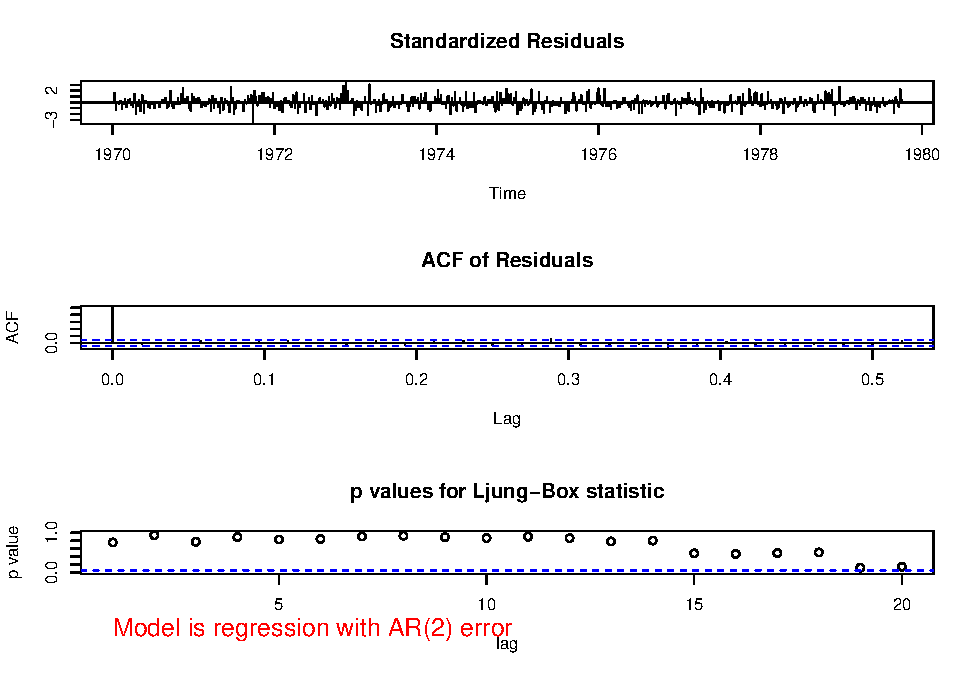
\includegraphics{02-Plotting_files/figure-latex/unnamed-chunk-10-1.pdf}

\begin{Shaded}
\begin{Highlighting}[]
\CommentTok{\# Autocorrelation}

\NormalTok{rho.x }\OtherTok{\textless{}{-}} \FunctionTok{acf}\NormalTok{(}\AttributeTok{x =}\NormalTok{ x, }\AttributeTok{type =} \StringTok{"correlation"}\NormalTok{, }\AttributeTok{main =} \StringTok{"OSU Enrollment series"}\NormalTok{)}
\end{Highlighting}
\end{Shaded}

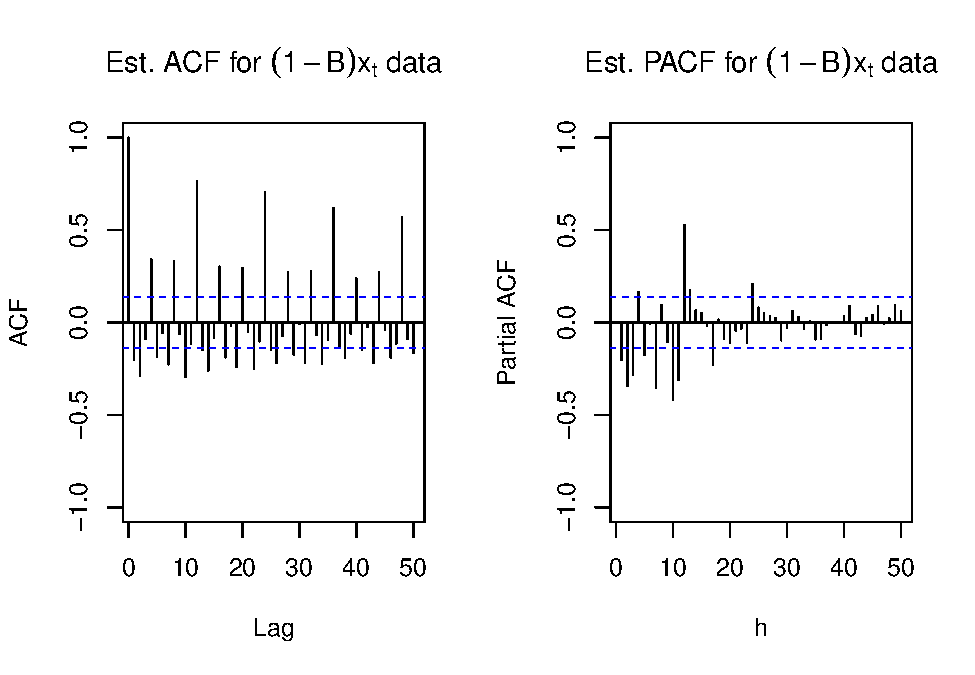
\includegraphics{02-Plotting_files/figure-latex/unnamed-chunk-11-1.pdf}

\begin{Shaded}
\begin{Highlighting}[]
\NormalTok{rho.x}
\end{Highlighting}
\end{Shaded}

\begin{verbatim}
## 
## Autocorrelations of series 'x', by lag
## 
##      0      1      2      3      4      5      6      7      8      9     10 
##  1.000 -0.470 -0.425  0.909 -0.438 -0.395  0.822 -0.403 -0.358  0.739 -0.367 
##     11     12     13     14     15     16 
## -0.327  0.655 -0.337 -0.297  0.581 -0.309
\end{verbatim}

\begin{Shaded}
\begin{Highlighting}[]
\NormalTok{rho.x}\SpecialCharTok{$}\NormalTok{acf[}\DecValTok{1}\SpecialCharTok{:}\DecValTok{9}\NormalTok{]}
\end{Highlighting}
\end{Shaded}

\begin{verbatim}
## [1]  1.0000000 -0.4702315 -0.4253427  0.9087421 -0.4377336 -0.3946048  0.8224660
## [8] -0.4025871 -0.3584216
\end{verbatim}

\hypertarget{sp500-index}{%
\section{S\&P500 Index}\label{sp500-index}}

Click \href{http://www.chrisbilder.com/stat878/sections/2/SP500weekly.csv}{SP500weekly.csv} to download data.

\begin{Shaded}
\begin{Highlighting}[]
\NormalTok{SP500 }\OtherTok{\textless{}{-}} \FunctionTok{read.csv}\NormalTok{(}\AttributeTok{file=}\StringTok{"SP500weekly.csv"}\NormalTok{,}\AttributeTok{stringsAsFactors =} \ConstantTok{TRUE}\NormalTok{)}
\end{Highlighting}
\end{Shaded}

\begin{Shaded}
\begin{Highlighting}[]
\FunctionTok{head}\NormalTok{(SP500)}
\end{Highlighting}
\end{Shaded}

\begin{verbatim}
##   WeekStart   Open   High    Low  Close AdjClose     Volume
## 1  1/1/1995 459.21 462.49 457.20 460.68   460.68 1199080000
## 2  1/8/1995 460.67 466.43 458.65 465.97   465.97 1627330000
## 3 1/15/1995 465.97 470.43 463.99 464.78   464.78 1667400000
## 4 1/22/1995 464.78 471.36 461.14 470.39   470.39 1628110000
## 5 1/29/1995 470.39 479.91 467.49 478.65   478.65 1888560000
## 6  2/5/1995 478.64 482.60 478.36 481.46   481.46 1579920000
\end{verbatim}

\begin{Shaded}
\begin{Highlighting}[]
\FunctionTok{tail}\NormalTok{(SP500)}
\end{Highlighting}
\end{Shaded}

\begin{verbatim}
##       WeekStart    Open    High     Low   Close AdjClose      Volume
## 1395  9/19/2021 4402.95 4465.40 4305.91 4455.48  4455.48 15697030000
## 1396  9/26/2021 4442.12 4457.30 4288.52 4357.04  4357.04 15555390000
## 1397  10/3/2021 4348.84 4429.97 4278.94 4391.34  4391.34 14795520000
## 1398 10/10/2021 4385.44 4475.82 4329.92 4471.37  4471.37 13758090000
## 1399 10/17/2021 4463.72 4559.67 4447.47 4544.90  4544.90 13966070000
## 1400 10/24/2021 4553.69 4608.08 4537.36 4605.38  4605.38 16206040000
\end{verbatim}

\begin{Shaded}
\begin{Highlighting}[]
\NormalTok{x }\OtherTok{\textless{}{-}}\NormalTok{ SP500}\SpecialCharTok{$}\NormalTok{Close}
\end{Highlighting}
\end{Shaded}

\begin{Shaded}
\begin{Highlighting}[]
\CommentTok{\#One way to do plot}
\FunctionTok{dev.new}\NormalTok{(}\AttributeTok{width =} \DecValTok{8}\NormalTok{, }\AttributeTok{height =} \DecValTok{6}\NormalTok{, }\AttributeTok{pointsize =} \DecValTok{10}\NormalTok{) }
\CommentTok{\#again, we do not specify y{-}axis here}
\FunctionTok{plot}\NormalTok{(}\AttributeTok{x =}\NormalTok{ x, }\AttributeTok{ylab =} \StringTok{"S\&P 500 Index"}\NormalTok{, }\AttributeTok{xlab =} \StringTok{"t (time)"}\NormalTok{, }
    \AttributeTok{type =} \StringTok{"l"}\NormalTok{, }\AttributeTok{col =} \StringTok{"red"}\NormalTok{, }\AttributeTok{main =} \StringTok{"S\&P 500 Index from }
\StringTok{    1/1/1995 to 10/25/2021 (weekly)"}\NormalTok{, }
    \AttributeTok{panel.first =} \FunctionTok{grid}\NormalTok{(}\AttributeTok{col =} \StringTok{"gray"}\NormalTok{, }\AttributeTok{lty =} \StringTok{"dotted"}\NormalTok{))}
\end{Highlighting}
\end{Shaded}

\begin{Shaded}
\begin{Highlighting}[]
\CommentTok{\#Another way to do plot with actual dates}
\FunctionTok{plot}\NormalTok{(}\AttributeTok{y =}\NormalTok{ x, }\AttributeTok{x =} \FunctionTok{as.Date}\NormalTok{(SP500}\SpecialCharTok{$}\NormalTok{WeekStart, }\AttributeTok{format =}
    \StringTok{"\%m/\%d/\%Y"}\NormalTok{), }\AttributeTok{xlab =} \StringTok{"Time"}\NormalTok{, }\AttributeTok{type =} \StringTok{"l"}\NormalTok{, }\AttributeTok{col =} \StringTok{"red"}\NormalTok{, main }
    \OtherTok{=} \StringTok{"S\&P 500 Index from 1/1/1995 to 10/25/2021 (weekly)"}\NormalTok{,}
    \AttributeTok{ylab =} \StringTok{"S\&P 500 Index"}\NormalTok{)}

\CommentTok{\#Create own gridlines}
\FunctionTok{abline}\NormalTok{(}\AttributeTok{v =} \FunctionTok{as.Date}\NormalTok{(}\FunctionTok{c}\NormalTok{(}\StringTok{"1995/1/1"}\NormalTok{, }\StringTok{"2000/1/1"}\NormalTok{, }\StringTok{"2005/1/1"}\NormalTok{, }
    \StringTok{"2010/1/1"}\NormalTok{, }\StringTok{"2015/1/1"}\NormalTok{, }\StringTok{"2020/1/1"}\NormalTok{)), }\AttributeTok{lty =} \StringTok{"dotted"}\NormalTok{, }
    \AttributeTok{col =} \StringTok{"lightgray"}\NormalTok{)}

\FunctionTok{abline}\NormalTok{(}\AttributeTok{h =} \FunctionTok{seq}\NormalTok{(}\AttributeTok{from =} \DecValTok{0}\NormalTok{, }\AttributeTok{to =} \DecValTok{5000}\NormalTok{, }\AttributeTok{by =} \DecValTok{1000}\NormalTok{), }\AttributeTok{lty =} 
    \StringTok{"dotted"}\NormalTok{, }\AttributeTok{col =} \StringTok{"lightgray"}\NormalTok{)}
\end{Highlighting}
\end{Shaded}

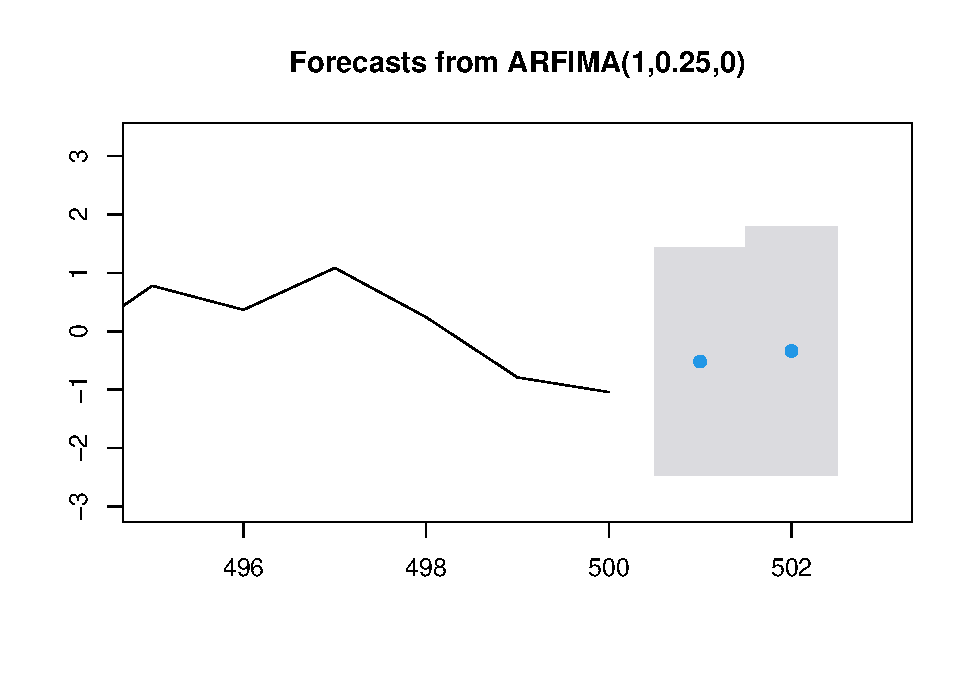
\includegraphics{02-Plotting_files/figure-latex/unnamed-chunk-17-1.pdf}

\begin{Shaded}
\begin{Highlighting}[]
\CommentTok{\# One more way with fine control of the dates}
\FunctionTok{plot}\NormalTok{(}\AttributeTok{y =}\NormalTok{ x, }\AttributeTok{x =} \FunctionTok{as.Date}\NormalTok{(SP500}\SpecialCharTok{$}\NormalTok{WeekStart, }\AttributeTok{format =} 
    \StringTok{"\%m/\%d/\%Y"}\NormalTok{), }\AttributeTok{xlab =} \StringTok{"Time"}\NormalTok{, }\AttributeTok{type =} \StringTok{"l"}\NormalTok{, }\AttributeTok{col =} \StringTok{"red"}\NormalTok{, }
    \AttributeTok{main =} \StringTok{"S\&P 500 Index from 1/1/1995 to 10/25/2021 }
\StringTok{    (weekly)"}\NormalTok{, }\AttributeTok{ylab =} \StringTok{"S\&P 500 Index"}\NormalTok{, }\AttributeTok{xaxt =} \StringTok{"n"}\NormalTok{)}

\FunctionTok{axis.Date}\NormalTok{(}\AttributeTok{side =} \DecValTok{1}\NormalTok{, }\AttributeTok{at =} \FunctionTok{seq}\NormalTok{(}\AttributeTok{from =} \FunctionTok{as.Date}\NormalTok{(}\StringTok{"1995/1/1"}\NormalTok{),}
    \AttributeTok{to =} \FunctionTok{as.Date}\NormalTok{(}\StringTok{"2021/12/31"}\NormalTok{), }\AttributeTok{by =} \StringTok{"years"}\NormalTok{), }\AttributeTok{labels =} 
    \FunctionTok{format}\NormalTok{(}\AttributeTok{x =} \FunctionTok{seq}\NormalTok{(}\AttributeTok{from =} \FunctionTok{as.Date}\NormalTok{(}\StringTok{"1995/1/1"}\NormalTok{), }\AttributeTok{to =} 
    \FunctionTok{as.Date}\NormalTok{(}\StringTok{"2021/12/31"}\NormalTok{), }\AttributeTok{by =} \StringTok{"years"}\NormalTok{), }\AttributeTok{format =} \StringTok{"\%b\%y"}\NormalTok{), }
    \AttributeTok{las =} \DecValTok{2}\NormalTok{)  }\CommentTok{\#las changes orientation of labels}

\CommentTok{\#Create own gridlines}
\FunctionTok{abline}\NormalTok{(}\AttributeTok{v =} \FunctionTok{as.Date}\NormalTok{(}\FunctionTok{c}\NormalTok{(}\StringTok{"1995/1/1"}\NormalTok{, }\StringTok{"2000/1/1"}\NormalTok{, }\StringTok{"2005/1/1"}\NormalTok{, }
    \StringTok{"2010/1/1"}\NormalTok{, }\StringTok{"2015/1/1"}\NormalTok{, }\StringTok{"2020/1/1"}\NormalTok{)), }\AttributeTok{lty =} \StringTok{"dotted"}\NormalTok{, }
    \AttributeTok{col =} \StringTok{"lightgray"}\NormalTok{)}
\FunctionTok{abline}\NormalTok{(}\AttributeTok{h =} \FunctionTok{seq}\NormalTok{(}\AttributeTok{from =} \DecValTok{0}\NormalTok{, }\AttributeTok{to =} \DecValTok{5000}\NormalTok{, }\AttributeTok{by =} \DecValTok{1000}\NormalTok{), }\AttributeTok{lty =} 
    \StringTok{"dotted"}\NormalTok{, }\AttributeTok{col =} \StringTok{"lightgray"}\NormalTok{)}
\end{Highlighting}
\end{Shaded}

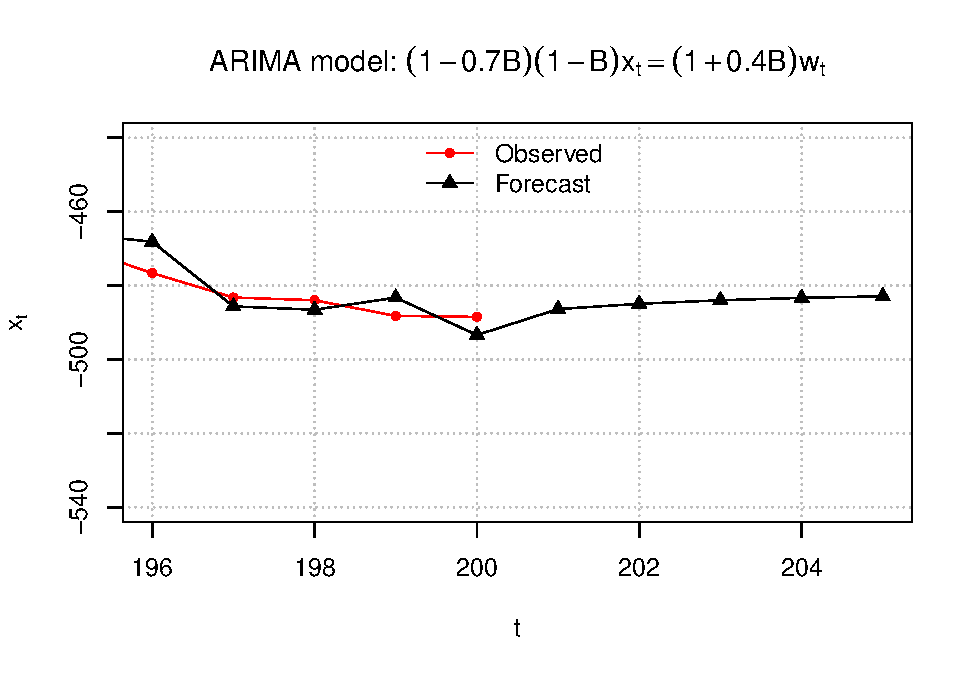
\includegraphics{02-Plotting_files/figure-latex/unnamed-chunk-18-1.pdf}

\hypertarget{sunspots}{%
\section{Sunspots}\label{sunspots}}

Click \href{http://www.chrisbilder.com/stat878/sections/2/SN_y_tot_V2.0.csv}{SN\_y\_tot\_V2.0.csv} to download data.

\begin{Shaded}
\begin{Highlighting}[]
\NormalTok{sunspots }\OtherTok{\textless{}{-}} \FunctionTok{read.table}\NormalTok{(}\AttributeTok{file =} \StringTok{"SN\_y\_tot\_V2.0.csv"}\NormalTok{, }\AttributeTok{sep =} 
    \StringTok{";"}\NormalTok{, }\AttributeTok{col.names =} \FunctionTok{c}\NormalTok{(}\StringTok{"Mid.year"}\NormalTok{, }\StringTok{"Mean.total"}\NormalTok{, }
   \StringTok{"Mean.SD.total"}\NormalTok{, }\StringTok{"Numb.obs.used"}\NormalTok{, }\StringTok{"Definitive"}\NormalTok{))}
\end{Highlighting}
\end{Shaded}

\begin{Shaded}
\begin{Highlighting}[]
\FunctionTok{head}\NormalTok{(sunspots)}
\end{Highlighting}
\end{Shaded}

\begin{verbatim}
##   Mid.year Mean.total Mean.SD.total Numb.obs.used Definitive
## 1   1700.5        8.3            -1            -1          1
## 2   1701.5       18.3            -1            -1          1
## 3   1702.5       26.7            -1            -1          1
## 4   1703.5       38.3            -1            -1          1
## 5   1704.5       60.0            -1            -1          1
## 6   1705.5       96.7            -1            -1          1
\end{verbatim}

\begin{Shaded}
\begin{Highlighting}[]
\FunctionTok{tail}\NormalTok{(sunspots)}
\end{Highlighting}
\end{Shaded}

\begin{verbatim}
##     Mid.year Mean.total Mean.SD.total Numb.obs.used Definitive
## 316   2015.5       69.8           6.4          8903          1
## 317   2016.5       39.8           3.9          9940          1
## 318   2017.5       21.7           2.5         11444          1
## 319   2018.5        7.0           1.1         12611          1
## 320   2019.5        3.6           0.5         12884          1
## 321   2020.5        8.8           4.1         14440          1
\end{verbatim}

\begin{Shaded}
\begin{Highlighting}[]
\FunctionTok{dev.new}\NormalTok{(}\AttributeTok{width =} \DecValTok{8}\NormalTok{, }\AttributeTok{height =} \DecValTok{6}\NormalTok{, }\AttributeTok{pointsize =} \DecValTok{10}\NormalTok{)}

\CommentTok{\#again, we did not specify y{-}axis here}
\FunctionTok{plot}\NormalTok{(}\AttributeTok{x =}\NormalTok{ sunspots}\SpecialCharTok{$}\NormalTok{Mean.total, }\AttributeTok{ylab =} \StringTok{"Number of }
\StringTok{    sunspots"}\NormalTok{, }\AttributeTok{xlab =} \StringTok{"t (time)"}\NormalTok{, }\AttributeTok{type =} \StringTok{"l"}\NormalTok{, }\AttributeTok{col =} \StringTok{"red"}\NormalTok{, }
    \AttributeTok{main =} \StringTok{"Sunspots per year from 1700 to 2020"}\NormalTok{,}
    \AttributeTok{panel.first =} \FunctionTok{grid}\NormalTok{(}\AttributeTok{col =} \StringTok{"gray"}\NormalTok{, }\AttributeTok{lty =} \StringTok{"dotted"}\NormalTok{))}

\FunctionTok{points}\NormalTok{(}\AttributeTok{x =}\NormalTok{ sunspots}\SpecialCharTok{$}\NormalTok{Mean.total, }\AttributeTok{pch =} \DecValTok{20}\NormalTok{, }\AttributeTok{col =} \StringTok{"blue"}\NormalTok{)}
\end{Highlighting}
\end{Shaded}

\begin{Shaded}
\begin{Highlighting}[]
\CommentTok{\# Include dates}
\FunctionTok{plot}\NormalTok{(}\AttributeTok{y =}\NormalTok{ sunspots}\SpecialCharTok{$}\NormalTok{Mean.total, }\AttributeTok{x =}\NormalTok{ sunspots}\SpecialCharTok{$}\NormalTok{Mid.year, ylab }
    \OtherTok{=} \StringTok{"Number of sunspots"}\NormalTok{, }\AttributeTok{xlab =} \StringTok{"Year"}\NormalTok{, }\AttributeTok{type =} \StringTok{"l"}\NormalTok{, col }
    \OtherTok{=} \StringTok{"red"}\NormalTok{, }\AttributeTok{main =} \StringTok{"Sunspots per year from 1700 to 2020"}\NormalTok{,}
    \AttributeTok{panel.first =} \FunctionTok{grid}\NormalTok{(}\AttributeTok{col =} \StringTok{"gray"}\NormalTok{, }\AttributeTok{lty =} \StringTok{"dotted"}\NormalTok{))}

\FunctionTok{points}\NormalTok{(}\AttributeTok{y =}\NormalTok{ sunspots}\SpecialCharTok{$}\NormalTok{Mean.total, }\AttributeTok{x =}\NormalTok{ sunspots}\SpecialCharTok{$}\NormalTok{Mid.year, }
    \AttributeTok{pch =} \DecValTok{20}\NormalTok{, }\AttributeTok{col =} \StringTok{"blue"}\NormalTok{)}
\end{Highlighting}
\end{Shaded}

\includegraphics{02-Plotting_files/figure-latex/unnamed-chunk-23-1.pdf}

\begin{Shaded}
\begin{Highlighting}[]
\CommentTok{\#Convert to an object of class "ts"}

\NormalTok{x }\OtherTok{\textless{}{-}} \FunctionTok{ts}\NormalTok{(}\AttributeTok{data =}\NormalTok{ sunspots}\SpecialCharTok{$}\NormalTok{Mean.total, }\AttributeTok{start =} \DecValTok{1700}\NormalTok{, frequency }
    \OtherTok{=} \DecValTok{1}\NormalTok{)}

\NormalTok{x}
\end{Highlighting}
\end{Shaded}

\begin{verbatim}
## Time Series:
## Start = 1700 
## End = 2020 
## Frequency = 1 
##   [1]   8.3  18.3  26.7  38.3  60.0  96.7  48.3  33.3  16.7  13.3   5.0   0.0
##  [13]   0.0   3.3  18.3  45.0  78.3 105.0 100.0  65.0  46.7  43.3  36.7  18.3
##  [25]  35.0  66.7 130.0 203.3 171.7 121.7  78.3  58.3  18.3   8.3  26.7  56.7
##  [37] 116.7 135.0 185.0 168.3 121.7  66.7  33.3  26.7   8.3  18.3  36.7  66.7
##  [49] 100.0 134.8 139.0  79.5  79.7  51.2  20.3  16.0  17.0  54.0  79.3  90.0
##  [61] 104.8 143.2 102.0  75.2  60.7  34.8  19.0  63.0 116.3 176.8 168.0 136.0
##  [73] 110.8  58.0  51.0  11.7  33.0 154.2 257.3 209.8 141.3 113.5  64.2  38.0
##  [85]  17.0  40.2 138.2 220.0 218.2 196.8 149.8 111.0 100.0  78.2  68.3  35.5
##  [97]  26.7  10.7   6.8  11.3  24.2  56.7  75.0  71.8  79.2  70.3  46.8  16.8
## [109]  13.5   4.2   0.0   2.3   8.3  20.3  23.2  59.0  76.3  68.3  52.9  38.5
## [121]  24.2   9.2   6.3   2.2  11.4  28.2  59.9  83.0 108.5 115.2 117.4  80.8
## [133]  44.3  13.4  19.5  85.8 192.7 227.3 168.7 143.0 105.5  63.3  40.3  18.1
## [145]  25.1  65.8 102.7 166.3 208.3 182.5 126.3 122.0 102.7  74.1  39.0  12.7
## [157]   8.2  43.4 104.4 178.3 182.2 146.6 112.1  83.5  89.2  57.8  30.7  13.9
## [169]  62.8 123.6 232.0 185.3 169.2 110.1  74.5  28.3  18.9  20.7   5.7  10.0
## [181]  53.7  90.5  99.0 106.1 105.8  86.3  42.4  21.8  11.2  10.4  11.8  59.5
## [193] 121.7 142.0 130.0 106.6  69.4  43.8  44.4  20.2  15.7   4.6   8.5  40.8
## [205]  70.1 105.5  90.1 102.8  80.9  73.2  30.9   9.5   6.0   2.4  16.1  79.0
## [217]  95.0 173.6 134.6 105.7  62.7  43.5  23.7   9.7  27.9  74.0 106.5 114.7
## [229] 129.7 108.2  59.4  35.1  18.6   9.2  14.6  60.2 132.8 190.6 182.6 148.0
## [241] 113.0  79.2  50.8  27.1  16.1  55.3 154.3 214.7 193.0 190.7 118.9  98.3
## [253]  45.0  20.1   6.6  54.2 200.7 269.3 261.7 225.1 159.0  76.4  53.4  39.9
## [265]  15.0  22.0  66.8 132.9 150.0 149.4 148.0  94.4  97.6  54.1  49.2  22.5
## [277]  18.4  39.3 131.0 220.1 218.9 198.9 162.4  91.0  60.5  20.6  14.8  33.9
## [289] 123.0 211.1 191.8 203.3 133.0  76.1  44.9  25.1  11.6  28.9  88.3 136.3
## [301] 173.9 170.4 163.6  99.3  65.3  45.8  24.7  12.6   4.2   4.8  24.9  80.8
## [313]  84.5  94.0 113.3  69.8  39.8  21.7   7.0   3.6   8.8
\end{verbatim}

\begin{Shaded}
\begin{Highlighting}[]
\FunctionTok{class}\NormalTok{(x)}
\end{Highlighting}
\end{Shaded}

\begin{verbatim}
## [1] "ts"
\end{verbatim}

\begin{Shaded}
\begin{Highlighting}[]
\FunctionTok{class}\NormalTok{(sunspots}\SpecialCharTok{$}\NormalTok{Mean.total)}
\end{Highlighting}
\end{Shaded}

\begin{verbatim}
## [1] "numeric"
\end{verbatim}

\hypertarget{plot.ts}{%
\subsection{plot.ts()}\label{plot.ts}}

plot() is a generic function - uses the plot.ts() method function

\begin{Shaded}
\begin{Highlighting}[]
\CommentTok{\# we did not specify y{-}axis here, but x is now ts}
\FunctionTok{plot}\NormalTok{(}\AttributeTok{x =}\NormalTok{ x, }\AttributeTok{ylab =} \FunctionTok{expression}\NormalTok{(}\FunctionTok{paste}\NormalTok{(x[t], }\StringTok{" (Number of }
\StringTok{   sunspots)"}\NormalTok{)), }\AttributeTok{xlab =} \StringTok{"Year"}\NormalTok{, }\AttributeTok{type =} \StringTok{"o"}\NormalTok{, }\AttributeTok{col =} \StringTok{"red"}\NormalTok{, main }
   \OtherTok{=} \StringTok{"Sunspots per year from 1700 to 2020"}\NormalTok{)}
\end{Highlighting}
\end{Shaded}

\begin{verbatim}
## Warning in title(main = main, xlab = xlab, ylab = ylab, ...): font metrics
## unknown for character 0xa

## Warning in title(main = main, xlab = xlab, ylab = ylab, ...): font metrics
## unknown for character 0xa
\end{verbatim}

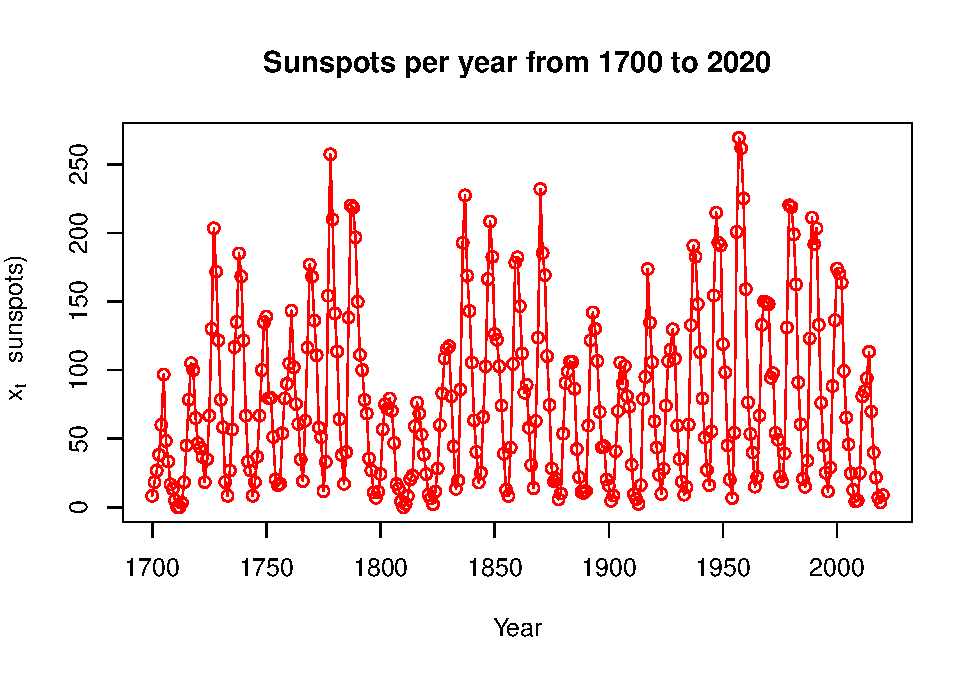
\includegraphics{02-Plotting_files/figure-latex/unnamed-chunk-26-1.pdf}

\begin{Shaded}
\begin{Highlighting}[]
\FunctionTok{plot.ts}\NormalTok{(}\AttributeTok{x =}\NormalTok{ x, }\AttributeTok{ylab =} \FunctionTok{expression}\NormalTok{(}\FunctionTok{paste}\NormalTok{(x[t], }\StringTok{" (Number of sunspots)"}\NormalTok{)),}
  \AttributeTok{xlab =} \StringTok{"Year"}\NormalTok{, }\AttributeTok{type =} \StringTok{"o"}\NormalTok{, }\AttributeTok{col =} \StringTok{"red"}\NormalTok{, }\AttributeTok{main =} \StringTok{"Sunspots per year from 1700 to 2020"}\NormalTok{)}
\end{Highlighting}
\end{Shaded}

\includegraphics{02-Plotting_files/figure-latex/unnamed-chunk-27-1.pdf}

\begin{Shaded}
\begin{Highlighting}[]
\CommentTok{\#type = "b" also works for "both" points and lines, but it leaves spaces between the points and lines}
\end{Highlighting}
\end{Shaded}

\hypertarget{basic-model}{%
\chapter{Basic Model}\label{basic-model}}

In this chapter, we will go introduce some basic \emph{Time Series} model. Hopefully, we can discuss them in details in the following chapters.

\begin{definition}
\textbf{\emph{Stochastic process}}

\textbf{\emph{Stochastic process}} is a collection of random variables \(\{X_t\}\) indexed by t.

\textbf{\emph{Time Series}} is a collection of random vatiables indexed according to the order they are obtained in time.

A \textbf{\emph{realization}} of the stochastic process is the observed values.
\end{definition}

\hypertarget{white-noise}{%
\section{White Noise}\label{white-noise}}

\begin{example}
\textbf{\emph{White Noise}}

\(W_t\sim \mathrm{i.i.d.} (0,\sigma^2) , \forall t=1,...,n\)

usually, we assume normal distribution, i.e.,

\(W_t\sim \mathrm{i.i.d.} N(0,\sigma^2) , \forall t=1,...,n\)
\end{example}

\begin{Shaded}
\begin{Highlighting}[]
\FunctionTok{set.seed}\NormalTok{(}\DecValTok{8128}\NormalTok{)}
\NormalTok{w }\OtherTok{\textless{}{-}} \FunctionTok{rnorm}\NormalTok{(}\AttributeTok{n =} \DecValTok{100}\NormalTok{, }\AttributeTok{mean =} \DecValTok{0}\NormalTok{, }\AttributeTok{sd =} \DecValTok{1}\NormalTok{)}
\FunctionTok{head}\NormalTok{(w)}
\end{Highlighting}
\end{Shaded}

\begin{verbatim}
## [1] -0.10528941  0.25548490  0.82065388  0.04070997 -0.66722880 -1.54502793
\end{verbatim}

\begin{Shaded}
\begin{Highlighting}[]
\FunctionTok{dev.new}\NormalTok{(}\AttributeTok{width =} \DecValTok{6}\NormalTok{, }\AttributeTok{height =} \DecValTok{6}\NormalTok{, }\AttributeTok{pointsize =} \DecValTok{10}\NormalTok{)}

\CommentTok{\# we did not specify y{-}axis here}
\CommentTok{\# note that we use expression() to type math expression}
\FunctionTok{plot}\NormalTok{(}\AttributeTok{x =}\NormalTok{ w, }\AttributeTok{ylab =} \FunctionTok{expression}\NormalTok{(w[t]), }\AttributeTok{xlab =} \StringTok{"t"}\NormalTok{, type }
    \OtherTok{=} \StringTok{"o"}\NormalTok{, }\AttributeTok{col =} \StringTok{"red"}\NormalTok{, }\AttributeTok{main =} \FunctionTok{expression}\NormalTok{(}\FunctionTok{paste}\NormalTok{(}\StringTok{"White }
\StringTok{    noise where "}\NormalTok{, w[t], }\StringTok{" \textasciitilde{} ind. N(0, 1)"}\NormalTok{)), }
    \AttributeTok{panel.first =} \FunctionTok{grid}\NormalTok{(}\AttributeTok{col =} \StringTok{"gray"}\NormalTok{, }\AttributeTok{lty =} \StringTok{"dotted"}\NormalTok{))}
\end{Highlighting}
\end{Shaded}

\begin{verbatim}
## Warning in title(...): font metrics unknown for character 0xa

## Warning in title(...): font metrics unknown for character 0xa
\end{verbatim}

\begin{Shaded}
\begin{Highlighting}[]
\CommentTok{\#Advantage of second plot is separate control over color of points}

\FunctionTok{plot}\NormalTok{(}\AttributeTok{x =}\NormalTok{ w, }\AttributeTok{ylab =} \FunctionTok{expression}\NormalTok{(w[t]), }\AttributeTok{xlab =} \StringTok{"t"}\NormalTok{, }\AttributeTok{type =} 
    \StringTok{"l"}\NormalTok{, }\AttributeTok{col =} \StringTok{"red"}\NormalTok{, }\AttributeTok{main =} \FunctionTok{expression}\NormalTok{(}\FunctionTok{paste}\NormalTok{(}\StringTok{"White noise where "}\NormalTok{, w[t], }\StringTok{" \textasciitilde{} ind. N(0, 1)"}\NormalTok{)), }
    \AttributeTok{panel.first =} \FunctionTok{grid}\NormalTok{(}\AttributeTok{col =} \StringTok{"gray"}\NormalTok{, }\AttributeTok{lty =} \StringTok{"dotted"}\NormalTok{))}

\FunctionTok{points}\NormalTok{(}\AttributeTok{x =}\NormalTok{ w, }\AttributeTok{pch =} \DecValTok{20}\NormalTok{, }\AttributeTok{col =} \StringTok{"blue"}\NormalTok{)}
\end{Highlighting}
\end{Shaded}

\includegraphics{03-Basic-Model_files/figure-latex/unnamed-chunk-3-1.pdf}

Suppose another white noise process is simulated. Below is a plot overlaying the two time series.

\begin{Shaded}
\begin{Highlighting}[]
\FunctionTok{set.seed}\NormalTok{(}\DecValTok{1298}\NormalTok{)}
\NormalTok{w.new }\OtherTok{\textless{}{-}} \FunctionTok{rnorm}\NormalTok{(}\AttributeTok{n =} \DecValTok{100}\NormalTok{, }\AttributeTok{mean =} \DecValTok{0}\NormalTok{, }\AttributeTok{sd =} \DecValTok{1}\NormalTok{)}
\FunctionTok{head}\NormalTok{(w.new)}
\end{Highlighting}
\end{Shaded}

\begin{verbatim}
## [1]  1.08820292 -1.46217413 -1.10887422  0.55156914  0.70582813  0.05079594
\end{verbatim}

\begin{Shaded}
\begin{Highlighting}[]
\FunctionTok{par}\NormalTok{(}\AttributeTok{mfrow=}\FunctionTok{c}\NormalTok{(}\DecValTok{1}\NormalTok{,}\DecValTok{1}\NormalTok{))}
\FunctionTok{plot}\NormalTok{(}\AttributeTok{x =}\NormalTok{ w, }
     \AttributeTok{ylab =} \FunctionTok{expression}\NormalTok{(w[t]), }\AttributeTok{xlab =} \StringTok{"t"}\NormalTok{, }
     \AttributeTok{type =} \StringTok{"l"}\NormalTok{, }\AttributeTok{col =} \StringTok{"red"}\NormalTok{,}
     \AttributeTok{main =} \FunctionTok{expression}\NormalTok{(}\FunctionTok{paste}\NormalTok{(}\StringTok{"White noise where "}\NormalTok{, w[t], }\StringTok{" \textasciitilde{} ind. N(0, 1)"}\NormalTok{)), }
     \AttributeTok{panel.first =} \FunctionTok{grid}\NormalTok{(}\AttributeTok{col =} \StringTok{"gray"}\NormalTok{, }\AttributeTok{lty =} \StringTok{"dotted"}\NormalTok{))}

\FunctionTok{points}\NormalTok{(}\AttributeTok{x =}\NormalTok{ w, }\AttributeTok{pch =} \DecValTok{20}\NormalTok{, }\AttributeTok{col =} \StringTok{"blue"}\NormalTok{)}

\FunctionTok{lines}\NormalTok{(}\AttributeTok{x =}\NormalTok{ w.new, }\AttributeTok{col =} \StringTok{"green"}\NormalTok{)}
\FunctionTok{points}\NormalTok{(}\AttributeTok{x =}\NormalTok{ w.new, }\AttributeTok{pch =} \DecValTok{20}\NormalTok{,}\AttributeTok{col =} \StringTok{"orange"}\NormalTok{)}
\FunctionTok{legend}\NormalTok{(}\AttributeTok{x =}\StringTok{"top"}\NormalTok{,}\AttributeTok{legend=}\FunctionTok{c}\NormalTok{(}\StringTok{"Time series 1"}\NormalTok{, }\StringTok{"Time series 2"}\NormalTok{), }\AttributeTok{lty=}\FunctionTok{c}\NormalTok{(}\DecValTok{1}\NormalTok{,}\DecValTok{1}\NormalTok{), }\AttributeTok{col=}\FunctionTok{c}\NormalTok{(}\StringTok{"red"}\NormalTok{, }\StringTok{"green"}\NormalTok{), }
      \AttributeTok{bty=}\StringTok{"n"}\NormalTok{)}
\end{Highlighting}
\end{Shaded}

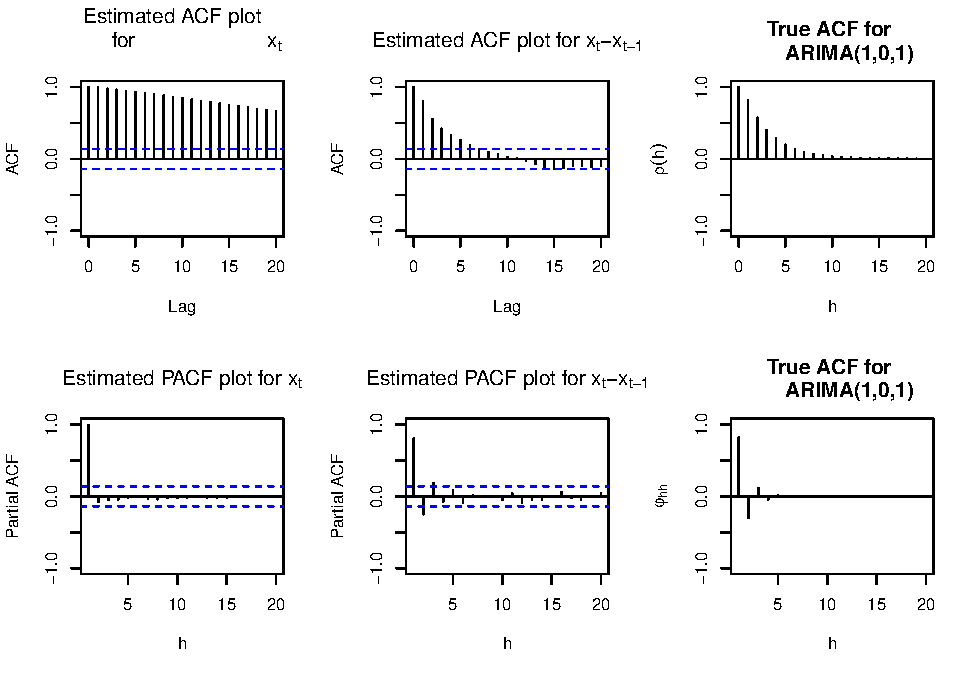
\includegraphics{03-Basic-Model_files/figure-latex/unnamed-chunk-5-1.pdf}

We could also plot the two time series separately.

\begin{Shaded}
\begin{Highlighting}[]
\FunctionTok{dev.new}\NormalTok{(}\AttributeTok{width =} \DecValTok{8}\NormalTok{, }\AttributeTok{height =} \DecValTok{6}\NormalTok{, }\AttributeTok{pointsize =} \DecValTok{10}\NormalTok{) }\CommentTok{\#Open a new plot window}
\CommentTok{\#make frame by row 2 rows 1 cols}
\FunctionTok{par}\NormalTok{(}\AttributeTok{mfrow =} \FunctionTok{c}\NormalTok{(}\DecValTok{2}\NormalTok{,}\DecValTok{1}\NormalTok{))}
\FunctionTok{plot}\NormalTok{(}\AttributeTok{x =}\NormalTok{ w, }\AttributeTok{ylab =} \FunctionTok{expression}\NormalTok{(w[t]), }\AttributeTok{xlab =} \StringTok{"t"}\NormalTok{, }\AttributeTok{type =} 
      \StringTok{"l"}\NormalTok{, }\AttributeTok{col =} \StringTok{"red"}\NormalTok{, }\AttributeTok{main =} \FunctionTok{expression}\NormalTok{(}\FunctionTok{paste}\NormalTok{(}\StringTok{"White noise where "}\NormalTok{, w[t], }\StringTok{"\textasciitilde{}N(0, 1)"}\NormalTok{)), }\AttributeTok{panel.first =} 
      \FunctionTok{grid}\NormalTok{(}\AttributeTok{col =} \StringTok{"gray"}\NormalTok{, }\AttributeTok{lty =} \StringTok{"dotted"}\NormalTok{))}
\FunctionTok{points}\NormalTok{(}\AttributeTok{x =}\NormalTok{ w, }\AttributeTok{pch =} \DecValTok{20}\NormalTok{, }\AttributeTok{col =} \StringTok{"blue"}\NormalTok{)}


\FunctionTok{plot}\NormalTok{(}\AttributeTok{x =}\NormalTok{ w.new, }\AttributeTok{ylab =} \FunctionTok{expression}\NormalTok{(w.new[t]), }\AttributeTok{xlab =} 
      \StringTok{"t"}\NormalTok{, }\AttributeTok{type =} \StringTok{"l"}\NormalTok{, }\AttributeTok{col =} \StringTok{"green"}\NormalTok{, }\AttributeTok{main =} 
      \FunctionTok{expression}\NormalTok{(}\FunctionTok{paste}\NormalTok{(}\StringTok{"White noise where "}\NormalTok{, w[t], }\StringTok{" \textasciitilde{} ind.N(0, 1)"}\NormalTok{)), }\AttributeTok{panel.first=}\FunctionTok{grid}\NormalTok{(}\AttributeTok{col =} \StringTok{"gray"}\NormalTok{, }\AttributeTok{lty =} 
      \StringTok{"dotted"}\NormalTok{))}
\FunctionTok{points}\NormalTok{(}\AttributeTok{x =}\NormalTok{ w.new, }\AttributeTok{pch =} \DecValTok{20}\NormalTok{, }\AttributeTok{col =} \StringTok{"orange"}\NormalTok{)}
\end{Highlighting}
\end{Shaded}

\begin{Shaded}
\begin{Highlighting}[]
\CommentTok{\# What if used plot.ts()?}
\FunctionTok{dev.new}\NormalTok{(}\AttributeTok{width =} \DecValTok{8}\NormalTok{, }\AttributeTok{height =} \DecValTok{6}\NormalTok{, }\AttributeTok{pointsize =} \DecValTok{10}\NormalTok{) }\CommentTok{\#Open a new plot window}

\FunctionTok{plot.ts}\NormalTok{(}\AttributeTok{x =} \FunctionTok{cbind}\NormalTok{(w, w.new), }\AttributeTok{ylab =} \FunctionTok{expression}\NormalTok{(w[t]), }\AttributeTok{xlab =} \StringTok{"t"}\NormalTok{, }\AttributeTok{type =} \StringTok{"o"}\NormalTok{, }\AttributeTok{col =} \StringTok{"red"}\NormalTok{, }\AttributeTok{main =} \FunctionTok{expression}\NormalTok{(}\FunctionTok{paste}\NormalTok{(}\StringTok{"White noise where "}\NormalTok{, w[t], }\StringTok{" \textasciitilde{} ind. N(0, 1)"}\NormalTok{)), }\AttributeTok{panel.first=}\FunctionTok{grid}\NormalTok{(}\AttributeTok{col =} \StringTok{"gray"}\NormalTok{, }\AttributeTok{lty =} \StringTok{"dotted"}\NormalTok{))}

\CommentTok{\#Problem: gridlines do not extend to second plot}
  
\FunctionTok{plot.ts}\NormalTok{(}\AttributeTok{x =} \FunctionTok{cbind}\NormalTok{(w, w.new), }\AttributeTok{ylab =} \FunctionTok{expression}\NormalTok{(w[t]), }\AttributeTok{xlab =} \StringTok{"t"}\NormalTok{, }\AttributeTok{type =} \StringTok{"o"}\NormalTok{, }\AttributeTok{col =} \StringTok{"red"}\NormalTok{, }\AttributeTok{main =} \FunctionTok{expression}\NormalTok{(}\FunctionTok{paste}\NormalTok{(}\StringTok{"White noise where "}\NormalTok{, w[t], }\StringTok{" \textasciitilde{} ind. N(0, 1)"}\NormalTok{)))}

\FunctionTok{grid}\NormalTok{(}\AttributeTok{col =} \StringTok{"gray"}\NormalTok{, }\AttributeTok{lty =} \StringTok{"dotted"}\NormalTok{)}
\CommentTok{\#Problem: gridlines do not appear correctly on plots (could fix by specifying where to draw them using abline)}
\end{Highlighting}
\end{Shaded}

\hypertarget{moving-average}{%
\section{Moving Average}\label{moving-average}}

\begin{example}
\textbf{\emph{Moving Average of White Noise}}

The previous time series had no correlation between the observations. One way to induce correlation is to create a ``moving average'' of the observations. This will have an effect of ``smoothing'' the series.

Let \(m_t = \frac{w_t+w_{t-1}+w_{t-2}}{3}\). This can be done in R using the following code:
\end{example}

\begin{Shaded}
\begin{Highlighting}[]
\FunctionTok{set.seed}\NormalTok{(}\DecValTok{8128}\NormalTok{)}
\NormalTok{w }\OtherTok{\textless{}{-}} \FunctionTok{rnorm}\NormalTok{(}\AttributeTok{n=}\DecValTok{100}\NormalTok{,}\AttributeTok{mean=}\DecValTok{0}\NormalTok{, }\AttributeTok{sd=}\DecValTok{1}\NormalTok{)}
\FunctionTok{head}\NormalTok{(w)}
\end{Highlighting}
\end{Shaded}

\begin{verbatim}
## [1] -0.10528941  0.25548490  0.82065388  0.04070997 -0.66722880 -1.54502793
\end{verbatim}

\begin{Shaded}
\begin{Highlighting}[]
\FunctionTok{dev.new}\NormalTok{(}\AttributeTok{width =} \DecValTok{8}\NormalTok{, }\AttributeTok{height =} \DecValTok{6}\NormalTok{, }\AttributeTok{pointsize =} \DecValTok{10}\NormalTok{) }\CommentTok{\#Open a new plot window}
\FunctionTok{plot}\NormalTok{(}\AttributeTok{x =}\NormalTok{ w, }\AttributeTok{ylab =} \FunctionTok{expression}\NormalTok{(}\FunctionTok{paste}\NormalTok{(m[t], }\StringTok{" or "}\NormalTok{, w[t])), }\AttributeTok{xlab =} \StringTok{"t"}\NormalTok{, }\AttributeTok{type =} \StringTok{"l"}\NormalTok{, }\AttributeTok{col =} \StringTok{"red"}\NormalTok{,}
        \AttributeTok{panel.first =} \FunctionTok{grid}\NormalTok{(}\AttributeTok{col =} \StringTok{"gray"}\NormalTok{, }\AttributeTok{lty =} \StringTok{"dotted"}\NormalTok{), }\AttributeTok{lty =} \StringTok{"dotted"}\NormalTok{)}
  \FunctionTok{points}\NormalTok{(}\AttributeTok{x =}\NormalTok{ w, }\AttributeTok{pch =} \DecValTok{20}\NormalTok{, }\AttributeTok{col =} \StringTok{"blue"}\NormalTok{)}
\end{Highlighting}
\end{Shaded}

\begin{Shaded}
\begin{Highlighting}[]
\CommentTok{\# rep(1/3,3) repeats 1/3 3 times}
\CommentTok{\# we can use filter() to generate moveing average}
\CommentTok{\# filter() help us build linear combination of elts of w}
\CommentTok{\# filter= linear combination coef}
\CommentTok{\# convolution for moving average}
\CommentTok{\# sides=1,表示只使用輸入向量的左側。}
\NormalTok{m }\OtherTok{\textless{}{-}} \FunctionTok{filter}\NormalTok{(w, }\AttributeTok{filter =} \FunctionTok{rep}\NormalTok{(}\DecValTok{1}\SpecialCharTok{/}\DecValTok{3}\NormalTok{, }\DecValTok{3}\NormalTok{), }\AttributeTok{method=}\StringTok{"convolution"}\NormalTok{, }\AttributeTok{sides=}\DecValTok{1}\NormalTok{)}

\FunctionTok{head}\NormalTok{(m)}
\end{Highlighting}
\end{Shaded}

\begin{verbatim}
## [1]          NA          NA  0.32361646  0.37228292  0.06471168 -0.72384892
\end{verbatim}

\begin{Shaded}
\begin{Highlighting}[]
\FunctionTok{tail}\NormalTok{(m)}
\end{Highlighting}
\end{Shaded}

\begin{verbatim}
## [1]  0.3158762 -0.1803096  0.2598066 -0.6450531 -0.5879723 -0.9120182
\end{verbatim}

\begin{Shaded}
\begin{Highlighting}[]
\NormalTok{(w[}\DecValTok{1}\NormalTok{]}\SpecialCharTok{+}\NormalTok{w[}\DecValTok{2}\NormalTok{]}\SpecialCharTok{+}\NormalTok{w[}\DecValTok{3}\NormalTok{])}\SpecialCharTok{/}\DecValTok{3}
\end{Highlighting}
\end{Shaded}

\begin{verbatim}
## [1] 0.3236165
\end{verbatim}

\begin{Shaded}
\begin{Highlighting}[]
\NormalTok{(w[}\DecValTok{98}\NormalTok{]}\SpecialCharTok{+}\NormalTok{w[}\DecValTok{99}\NormalTok{]}\SpecialCharTok{+}\NormalTok{w[}\DecValTok{100}\NormalTok{])}\SpecialCharTok{/}\DecValTok{3}
\end{Highlighting}
\end{Shaded}

\begin{verbatim}
## [1] -0.9120182
\end{verbatim}

\begin{Shaded}
\begin{Highlighting}[]
\FunctionTok{plot}\NormalTok{(}\AttributeTok{x =}\NormalTok{ w, }\AttributeTok{ylab =} \FunctionTok{expression}\NormalTok{(}\FunctionTok{paste}\NormalTok{(m[t], }\StringTok{" or "}\NormalTok{, w[t])), }
    \AttributeTok{xlab =} \StringTok{"t"}\NormalTok{, }\AttributeTok{type =} \StringTok{"l"}\NormalTok{, }\AttributeTok{col =} \StringTok{"red"}\NormalTok{, }\AttributeTok{panel.first =} 
    \FunctionTok{grid}\NormalTok{(}\AttributeTok{col =} \StringTok{"gray"}\NormalTok{, }\AttributeTok{lty =} \StringTok{"dotted"}\NormalTok{), }\AttributeTok{lty =} \StringTok{"dotted"}\NormalTok{)}
\FunctionTok{points}\NormalTok{(}\AttributeTok{x =}\NormalTok{ w, }\AttributeTok{pch =} \DecValTok{20}\NormalTok{, }\AttributeTok{col =} \StringTok{"blue"}\NormalTok{)}
\FunctionTok{lines}\NormalTok{(}\AttributeTok{x =}\NormalTok{ m, }\AttributeTok{col =} \StringTok{"brown"}\NormalTok{, }\AttributeTok{lty =} \StringTok{"solid"}\NormalTok{, }\AttributeTok{lwd =} \DecValTok{4}\NormalTok{)}
\FunctionTok{points}\NormalTok{(}\AttributeTok{x =}\NormalTok{ m, }\AttributeTok{pch =} \DecValTok{20}\NormalTok{, }\AttributeTok{col =} \StringTok{"orange"}\NormalTok{)}
\FunctionTok{legend}\NormalTok{(}\AttributeTok{x =} \StringTok{"top"}\NormalTok{, }\AttributeTok{legend =} \FunctionTok{c}\NormalTok{(}\StringTok{"MA, 3 points"}\NormalTok{, }\StringTok{"White noise"}\NormalTok{), }\AttributeTok{lty =} \FunctionTok{c}\NormalTok{(}\StringTok{"solid"}\NormalTok{, }\StringTok{"dotted"}\NormalTok{), }\AttributeTok{col=}\FunctionTok{c}\NormalTok{(}\StringTok{"brown"}\NormalTok{, }
    \StringTok{"red"}\NormalTok{), }\AttributeTok{lwd =} \FunctionTok{c}\NormalTok{(}\DecValTok{4}\NormalTok{,}\DecValTok{1}\NormalTok{), }\AttributeTok{bty =} \StringTok{"n"}\NormalTok{)}
\end{Highlighting}
\end{Shaded}

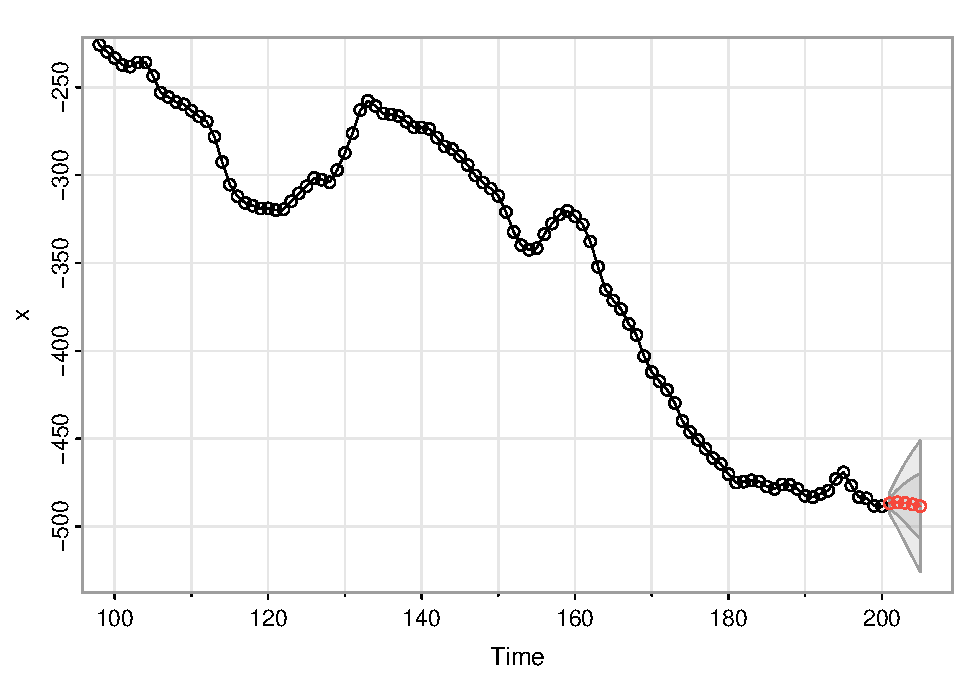
\includegraphics{03-Basic-Model_files/figure-latex/unnamed-chunk-12-1.pdf}

The plot below shows a 7-point moving average.

\begin{Shaded}
\begin{Highlighting}[]
\NormalTok{m7 }\OtherTok{\textless{}{-}} \FunctionTok{filter}\NormalTok{(}\AttributeTok{x=}\NormalTok{w, }\AttributeTok{filter=}\FunctionTok{rep}\NormalTok{(}\AttributeTok{x=}\DecValTok{1}\SpecialCharTok{/}\DecValTok{7}\NormalTok{, }\AttributeTok{times=}\DecValTok{7}\NormalTok{),}\AttributeTok{method=}\StringTok{"convolution"}\NormalTok{, }\AttributeTok{sides=}\DecValTok{1}\NormalTok{)}

\FunctionTok{plot}\NormalTok{(}\AttributeTok{x=}\NormalTok{w, }\AttributeTok{ylab=}\FunctionTok{expression}\NormalTok{(}\FunctionTok{paste}\NormalTok{(m[t],}\StringTok{"or"}\NormalTok{,w[t])), }\AttributeTok{xlab=}\StringTok{"t"}\NormalTok{,}\AttributeTok{type=}\StringTok{"l"}\NormalTok{,}\AttributeTok{col=}\StringTok{"red"}\NormalTok{,}\AttributeTok{panel\_filter=}\FunctionTok{grid}\NormalTok{(}\AttributeTok{col=}\StringTok{"gray"}\NormalTok{,}\AttributeTok{lty=}\StringTok{"dotted"}\NormalTok{), }\AttributeTok{lty=}\StringTok{"dotted"}\NormalTok{)}

\FunctionTok{points}\NormalTok{(}\AttributeTok{x=}\NormalTok{w, }\AttributeTok{pch=}\DecValTok{20}\NormalTok{, }\AttributeTok{col=}\StringTok{"blue"}\NormalTok{)}

\FunctionTok{lines}\NormalTok{(}\AttributeTok{x=}\NormalTok{m, }\AttributeTok{col=}\StringTok{"brown"}\NormalTok{, }\AttributeTok{lty=}\StringTok{"solid"}\NormalTok{,}\AttributeTok{lwd=}\DecValTok{4}\NormalTok{)}

\FunctionTok{points}\NormalTok{(}\AttributeTok{x=}\NormalTok{m, }\AttributeTok{pch=}\DecValTok{20}\NormalTok{, }\AttributeTok{col=}\StringTok{"orange"}\NormalTok{)}
\FunctionTok{lines}\NormalTok{(}\AttributeTok{x =}\NormalTok{ m7, }\AttributeTok{col =} \StringTok{"lightgreen"}\NormalTok{, }\AttributeTok{lty =} \StringTok{"solid"}\NormalTok{, }\AttributeTok{lwd =} \DecValTok{4}\NormalTok{)}
\FunctionTok{points}\NormalTok{(}\AttributeTok{x =}\NormalTok{ m7, }\AttributeTok{pch =} \DecValTok{20}\NormalTok{, }\AttributeTok{col =} \StringTok{"darkgreen"}\NormalTok{)}

\FunctionTok{legend}\NormalTok{(}\AttributeTok{x =} \StringTok{"top"}\NormalTok{, }\AttributeTok{legend =} \FunctionTok{c}\NormalTok{(}\StringTok{"MA, 3 points"}\NormalTok{, }\StringTok{"White noise"}\NormalTok{, }\StringTok{"MA 7 points"}\NormalTok{),}
         \AttributeTok{lty =} \FunctionTok{c}\NormalTok{(}\StringTok{"solid"}\NormalTok{, }\StringTok{"dotted"}\NormalTok{, }\StringTok{"solid"}\NormalTok{), }\AttributeTok{col =} \FunctionTok{c}\NormalTok{(}\StringTok{"brown"}\NormalTok{, }\StringTok{"red"}\NormalTok{, }\StringTok{"lightgreen"}\NormalTok{),}
         \AttributeTok{lwd =} \FunctionTok{c}\NormalTok{(}\DecValTok{2}\NormalTok{,}\DecValTok{1}\NormalTok{,}\DecValTok{4}\NormalTok{), }\AttributeTok{bty=}\StringTok{"n"}\NormalTok{)}
\end{Highlighting}
\end{Shaded}

\includegraphics{03-Basic-Model_files/figure-latex/unnamed-chunk-13-1.pdf}

\hypertarget{autoregression}{%
\section{Autoregression}\label{autoregression}}

\begin{example}
\textbf{\emph{Autoregression}}

An autoregression model uses past observations to predict future observations in a regression model.

Suppose the autoregression model is

\(x_t = 0.7x_{t-1} + w_t, w_t \sim \mathrm{i.i.d.} N(0,1) ,\forall t = 1, …, n\)

Because there is one past period on the right hand side, this is often denoted as an AR(1) model

Obviously, there will be a correlation between the random variables.
\end{example}

\begin{Shaded}
\begin{Highlighting}[]
\FunctionTok{set.seed}\NormalTok{(}\DecValTok{6381}\NormalTok{)  }\CommentTok{\#Different seed from white\_noise.R}
\NormalTok{w }\OtherTok{\textless{}{-}} \FunctionTok{rnorm}\NormalTok{(}\AttributeTok{n =} \DecValTok{200}\NormalTok{, }\AttributeTok{mean =} \DecValTok{0}\NormalTok{, }\AttributeTok{sd =} \DecValTok{1}\NormalTok{)}
\FunctionTok{head}\NormalTok{(w)}
\end{Highlighting}
\end{Shaded}

\begin{verbatim}
## [1]  0.06737166 -0.68095839  0.78930605  0.60049855 -1.21297680 -1.14082872
\end{verbatim}

\begin{Shaded}
\begin{Highlighting}[]
\CommentTok{\#Simple way to simulate AR(1) data}
\NormalTok{x }\OtherTok{\textless{}{-}} \FunctionTok{numeric}\NormalTok{(}\AttributeTok{length =} \DecValTok{200}\NormalTok{)}
\NormalTok{x}\FloatTok{.1} \OtherTok{\textless{}{-}} \DecValTok{0}
\ControlFlowTok{for}\NormalTok{(i }\ControlFlowTok{in} \DecValTok{1}\SpecialCharTok{:}\FunctionTok{length}\NormalTok{(x)) \{}
\NormalTok{    x[i] }\OtherTok{\textless{}{-}} \FloatTok{0.7}\SpecialCharTok{*}\NormalTok{x}\FloatTok{.1} \SpecialCharTok{+}\NormalTok{ w[i]}
\NormalTok{    x}\FloatTok{.1} \OtherTok{\textless{}{-}}\NormalTok{ x[i]}
\NormalTok{  \}}
\end{Highlighting}
\end{Shaded}

\begin{Shaded}
\begin{Highlighting}[]
\FunctionTok{head}\NormalTok{(}\FunctionTok{data.frame}\NormalTok{(x, w))}
\end{Highlighting}
\end{Shaded}

\begin{verbatim}
##             x           w
## 1  0.06737166  0.06737166
## 2 -0.63379823 -0.68095839
## 3  0.34564730  0.78930605
## 4  0.84245166  0.60049855
## 5 -0.62326064 -1.21297680
## 6 -1.57711117 -1.14082872
\end{verbatim}

\begin{Shaded}
\begin{Highlighting}[]
\CommentTok{\#Do not use first 100}
\NormalTok{x }\OtherTok{\textless{}{-}}\NormalTok{ x[}\DecValTok{101}\SpecialCharTok{:}\DecValTok{200}\NormalTok{]}
\end{Highlighting}
\end{Shaded}

\begin{Shaded}
\begin{Highlighting}[]
\FunctionTok{dev.new}\NormalTok{(}\AttributeTok{width =} \DecValTok{8}\NormalTok{, }\AttributeTok{height =} \DecValTok{6}\NormalTok{, }\AttributeTok{pointsize =} \DecValTok{10}\NormalTok{)  }\CommentTok{\#Opens up wider plot window than the default (good for time series plots)}
\FunctionTok{plot}\NormalTok{(}\AttributeTok{x =}\NormalTok{ x, }\AttributeTok{ylab =} \FunctionTok{expression}\NormalTok{(x[t]), }\AttributeTok{xlab =} \StringTok{"t"}\NormalTok{, }\AttributeTok{type =} 
      \StringTok{"l"}\NormalTok{, }\AttributeTok{col =} \FunctionTok{c}\NormalTok{(}\StringTok{"red"}\NormalTok{), }\AttributeTok{lwd =} \DecValTok{1}\NormalTok{ , }\AttributeTok{main =} 
      \FunctionTok{expression}\NormalTok{(}\FunctionTok{paste}\NormalTok{(}\StringTok{"AR(1): "}\NormalTok{, x[t] }\SpecialCharTok{==} \FloatTok{0.7}\SpecialCharTok{*}\NormalTok{x[t}\DecValTok{{-}1}\NormalTok{] }\SpecialCharTok{+} 
\NormalTok{      w[t])), }\AttributeTok{panel.first =} \FunctionTok{grid}\NormalTok{(}\AttributeTok{col =} \StringTok{"gray"}\NormalTok{, }\AttributeTok{lty =} 
      \StringTok{"dotted"}\NormalTok{))}
\FunctionTok{points}\NormalTok{(}\AttributeTok{x =}\NormalTok{ x, }\AttributeTok{pch =} \DecValTok{20}\NormalTok{, }\AttributeTok{col =} \StringTok{"blue"}\NormalTok{)}
\end{Highlighting}
\end{Shaded}

\begin{Shaded}
\begin{Highlighting}[]
 \CommentTok{\#Show first few observations after removal of first 100}
  \FunctionTok{head}\NormalTok{(}\FunctionTok{data.frame}\NormalTok{(}\FunctionTok{c}\NormalTok{(}\ConstantTok{NA}\NormalTok{, }\ConstantTok{NA}\NormalTok{, x), w[}\DecValTok{99}\SpecialCharTok{:}\DecValTok{200}\NormalTok{]))}
\end{Highlighting}
\end{Shaded}

\begin{verbatim}
##   c.NA..NA..x.  w.99.200.
## 1           NA  0.3918531
## 2           NA -0.1980565
## 3     1.429572  0.7508375
## 4    -1.878239 -2.8789389
## 5    -1.470250 -0.1554829
## 6    -3.464078 -2.4349033
\end{verbatim}

\begin{Shaded}
\begin{Highlighting}[]
  \CommentTok{\#Correlation between x\_t and x\_t{-}1 }
  \FunctionTok{cor}\NormalTok{(x[}\DecValTok{2}\SpecialCharTok{:}\DecValTok{100}\NormalTok{], x[}\DecValTok{1}\SpecialCharTok{:}\DecValTok{99}\NormalTok{])}
\end{Highlighting}
\end{Shaded}

\begin{verbatim}
## [1] 0.7270483
\end{verbatim}

Here is an easier way to simulate observations from an AR(1). Note that this uses an Autoregressive Integrated Moving Average (ARIMA) structure that we will discuss later in the course. In this case, I use \(\sigma_w\)= 10.

\begin{Shaded}
\begin{Highlighting}[]
\FunctionTok{set.seed}\NormalTok{(}\DecValTok{7181}\NormalTok{)}
\NormalTok{x }\OtherTok{\textless{}{-}} \FunctionTok{arima.sim}\NormalTok{(}\AttributeTok{model =} \FunctionTok{list}\NormalTok{(}\AttributeTok{ar =} \FunctionTok{c}\NormalTok{(}\FloatTok{0.7}\NormalTok{)), }\AttributeTok{n =} \DecValTok{100}\NormalTok{, }
    \AttributeTok{rand.gen =}\NormalTok{ rnorm, }\AttributeTok{sd =} \DecValTok{10}\NormalTok{)}
\FunctionTok{plot}\NormalTok{(}\AttributeTok{x =}\NormalTok{ x, }\AttributeTok{ylab =} \FunctionTok{expression}\NormalTok{(x[t]), }\AttributeTok{xlab =} \StringTok{"t"}\NormalTok{, }\AttributeTok{type =} 
    \StringTok{"l"}\NormalTok{, }\AttributeTok{col =} \StringTok{"red"}\NormalTok{, }\AttributeTok{lwd =} \DecValTok{1}\NormalTok{ ,}\AttributeTok{main =} 
    \FunctionTok{expression}\NormalTok{(}\FunctionTok{paste}\NormalTok{(}\StringTok{"AR(1): "}\NormalTok{, x[t] }\SpecialCharTok{==} \FloatTok{0.7}\SpecialCharTok{*}\NormalTok{x[t}\DecValTok{{-}1}\NormalTok{] }\SpecialCharTok{+} 
\NormalTok{    w[t])), }\AttributeTok{panel.first=}\FunctionTok{grid}\NormalTok{(}\AttributeTok{col =} \StringTok{"gray"}\NormalTok{, }\AttributeTok{lty =} 
    \StringTok{"dotted"}\NormalTok{))}
\FunctionTok{points}\NormalTok{(}\AttributeTok{x =}\NormalTok{ x, }\AttributeTok{pch =} \DecValTok{20}\NormalTok{, }\AttributeTok{col =} \StringTok{"blue"}\NormalTok{)}
\end{Highlighting}
\end{Shaded}

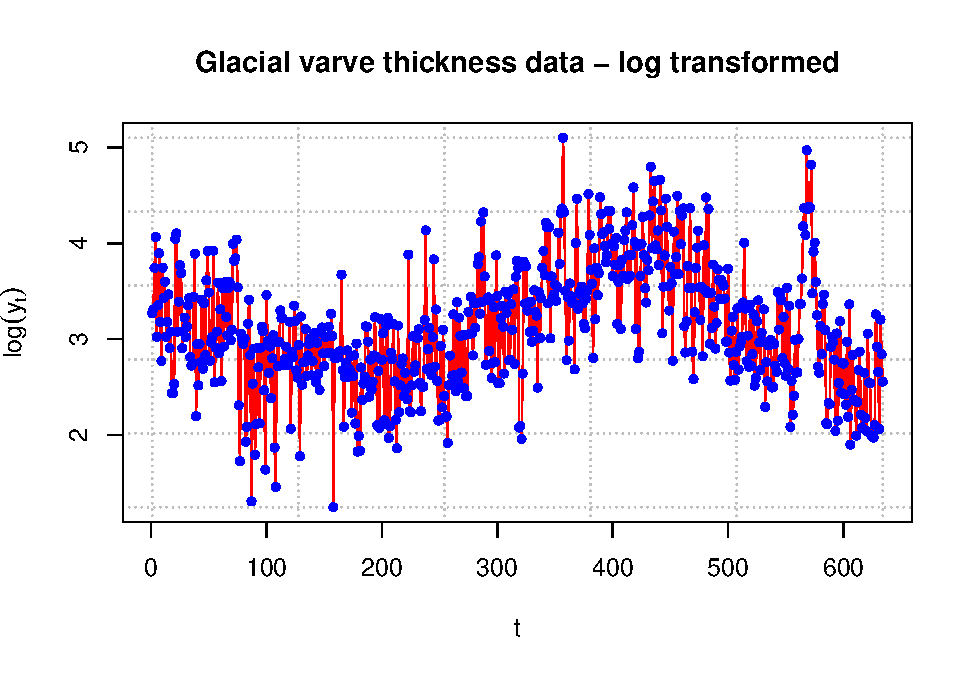
\includegraphics{03-Basic-Model_files/figure-latex/unnamed-chunk-20-1.pdf}

\hypertarget{dependence}{%
\chapter{Dependence}\label{dependence}}

We would like to understand the relationship among all random variables in a time series. In order to do that, we would need to look at the joint distribution function.

Suppose the time series consists of the random variables . The cumulative joint distribution function for these random variables is:

\[ F(c_1, c_2, …, c_n) = P(X_1\leq{c_1},X_2\leq{c_2},...,X_n\leq{c_n}) \]

This can be VERY difficult to examine over the MULTIDIMENSIONS.

The one-dimensional cumulative distributional function is denoted by \(F_t(x) = P(X_t\leq{x})\)for a random variable \(X_t\) at time t. The corresponding probability distribution function is \(f_t(x)=\frac{\partial{F_t(x)}}{\partial{x}}\)

The mean value function is \(\mu_t=E(X_t)=\int{xf_t(x)dx}\)

Important: The interpretation of \(\mu_t\) is that it represents the mean taken over ALL possible events that could have produced \(x_t\). Another way to think about it is suppose that \(x_1,\dots,x_n\) is observed an infinite number of times. Then \(\mu_1\) represents the average value at time 1, \(\mu_2\) represents the average value at time 2, \ldots{}

\begin{example}
\textbf{Moving Average}

Let \(m_t=\frac{(w_t+w_{t-1}+w_{t-2})}{3}\), where \(w_t\sim\mathrm{i.i.d.}N(0,1)\forall t=1,...,n\)

Then \(\mu_t=E(m_t)=E[\frac{(w_t+w_{t-1}+w_{t-2})}{3}]=\frac{1}{3}[E(w_t)+E(w_{t-1})+E(w_{t-2})]=0\)
\end{example}

\begin{example}
\textbf{Autoregressions}

Let \(x_t = 0.7x_{t-1} + w_t, w_t \sim \mathrm{i.i.d.} N(0,1) ,\forall t = 1, …, n\)

Then \(\mu_t=E(x_t)=E[0.7x_{t-1} + w_t]=0.7E(x_{t-1})+E(w_t)=0.7E(0.7x_{t-2}+w_{t-1})+0=...=0\)
\end{example}

\hypertarget{autocovariance-function}{%
\section{Autocovariance function}\label{autocovariance-function}}

To assess the dependence between two random variables, we need to examine the two-dimensional cumulative distribution function. This can be denoted as \(F(c_s, c_t) = P(X_s\leq{c_s}, X_t\leq{c_t})\)for two different time points s and t.

In another course, you learned about the covariance function which measures the linear dependence between two random variables:For two random variables X and Y, the covariance between them is

\[Cov(X,Y) = E[(X – \mu_x)(Y – \mu_y)] = E(XY) – \mu_x\mu_y,  
\mu_x = E(X) , \mu_y = E(Y)\]

Because we are interested in linear dependence between two random variables in the same time series, we will examine the autocovariance function:

\[\gamma (s,t)  = Cov(X_s, X_t)
= E[(X_s – \mu_s)(X_t – \mu_t)]=
\int\int(x_s-\mu_s)(x_t-\mu_t)f(x_s,x_t)dx_sdx_t ,\forall s, t \]

where\(f(X_s,X_t)=\frac{\partial{F(X_s,X_t)}}{\partial{X_s}\partial{X_t}}\)and assuming continuous random variables

\begin{itemize}
\tightlist
\item
  If the autocovariance is 0, there is no linear dependence.\\
\item
  If s = t, the autocovariance is the variance:\\
  \(\gamma (t,t) = E[(X_t-\mu_t)^2]\)
\end{itemize}

\begin{example}
\textbf{White Noise}

Suppose \(w_t \sim ind. N(0,\sigma^2_w ), t=1,…,n.\)

\[\begin{cases}
  \gamma(s,t)=\sigma^2_w  & \text{if } s=t \\
  \gamma(s,t)= 0  & \text{if } s\ne t
\end{cases}\]
\end{example}

\begin{example}
\textbf{Moving Average}

Let \(m_t=\frac{w_t+w_{t-1}+w_{t-2}}{3}, w_t \sim ind. N(0,1 ), t=1,…,n\)

\(\gamma (s,t)=E[(m_s-\mu_s)(m_t-\mu_t)]=E[m_sm_t]\) b/c \(\mu_s=\mu_t=0\)

Then \(E[m_sm_t]=E[\frac{w_s+w_{s-1}+w_{s-2}}{3}\frac{w_t+w_{t-1}+w_{t-2}}{3}]=\frac{1}{9}E[(w_s+w_{s-1}+w_{s-2})(w_t+w_{t-1}+w_{t-2})]\)

To find this, we need to examine a few different cases:

\begin{itemize}
\tightlist
\item
  s = t
\end{itemize}

\[E[m_tm_t] = E[m^2_t] = Var(m_t) + [E(m_t)]^2 
= \frac{1}{9}Var(w_t + w_{t-1} + w_{t-2}) + 0\\= \frac{1}{9}{Var(w_t) + Var(w_{t-1}) + Var(w_{t-2})} = \frac{1}{9}(1+1+1) = 3/9\]

\begin{itemize}
\tightlist
\item
  s = t - 1
\end{itemize}

\[E[m_{t-1}m_t] =\frac{1}{9}E[(w_{t-1} + w_{t-2} + w_{t-3})(w_t + w_{t-1} + w_{t-2})]\\
= \frac{1}{9}[E(w_{t-1})E(w_t) + E(w^2_{t-1}) + E(w_{t-1})E(w_{t-2}) \\
+ E(w_{t-2})E(w_t) + E(w_{t-2})E(w_{t-1}) + E(w^2_{t-2}) \\
+ E(w_{t-3})E(w_t) + E(w_{t-3})E(w_{t-1}) + E(w_{t-3})E(w_{t-2})]\\
=\frac{1}{9}[0 + 1 + 0 + 0 + 0 + 1 + 0  + 0  + 0]=2/9\]
\(E(w^2_{t-1}) = 1\), because \(Var(w_{t-1}) = 1\)

\begin{itemize}
\tightlist
\item
  s = t - 2
\end{itemize}

\[E[m_{t-2}m_t] = \frac{1}{9}E[(w_{t-2} + w_{t-3} + w_{t-4})(w_t + w_{t-1} + w_{t-2})]\\
= \frac{1}{9}[E(w_{t-2}w_t) + E(w_{t-2}w_{t-1}) + E(w_{t-2}w_{t-2}) +\\ E(w_{t-3}w_t) + E(w_{t-3}w_{t-1}) + E(w_{t-3}w_{t-2})\\ + E(w_{t-4}w_t) 
+ E(w_{t-4}w_{t-1}) + E(w_{t-4}w_{t-2})]\\
=\frac{1}{9}[0 + 0 + 0 + 1 + 0 + 0  + 0  + 0 + 0]
=\frac{1}{9}\]

\begin{itemize}
\tightlist
\item
  s = t -- 3
\end{itemize}

\[ E[m_{t-3}m_t] = \frac{1}{9}E[(w_{t-3} + w_{t-4} + w_{t-5})(w_t + w_{t-1} + w_{t-2})]\\
= \frac{1}{9}E[w_{t-3}w_t + w_{t-3}w_{t-1} + w_{t-3}w_{t-2} + w_{t-4}w_t + w_{t-4}w_{t-1} \\
+ w_{t-4}w_{t-2} + w_{t-5}w_t + w_{t-5}w_{t-1} + w_{t-5}w_{t-2}]\\
= \frac{1}{9}E[0+ 0 + 0 + 0 + 0 + 0  + 0 + 0 + 0]= 0 \]
\end{example}

Notice that s = t + 1, t + 2, \ldots{} can be found in a similar manner. Also s = t - 4, t - 5,\ldots{} can be found. In summary, the autocovariance function is\[\begin{cases}
  \gamma(s,t)= \frac{3}{9} & \text{if } s=t \\
  \gamma(s,t)= \frac{2}{9} & \text{if } |s-t|=1\\
  \gamma(s,t)= \frac{1}{9} & \text{if } |s-t|=2\\
  \gamma(s,t)= 0 & \text{if } |s-t|\ge 3\\
\end{cases}\]

Notes:
- The word ``lag'' is used to denote the time separation between two values. For example, \textbar s - t\textbar{} = 1 denotes the lag is 1 and \textbar s - t\textbar{} = 2 denotes the lag is 2. We will use this ``lag'' terminology throughout this course.

\begin{itemize}
\tightlist
\item
  The autocovariance depends on the lag, but NOT individual times for the moving average example! This will be VERY, VERY important later!
\end{itemize}

\hypertarget{autocorrelation-function-acf}{%
\section{Autocorrelation function (ACF)}\label{autocorrelation-function-acf}}

In another course, the Pearson correlation coefficient was defined to be:

\[\rho=\frac{Cov(X,Y)}{\sqrt{Var(X)Var(Y)}}\]

The reason the correlation coefficient is examined instead of the covariance is that it is always between --1 and 1.

Note the following:

\begin{itemize}
\tightlist
\item
  close to 1 means strong, positive linear dependence
\item
  close to --1 means strong, negative linear dependence
\item
  close to 0 means weak linear dependence.
\end{itemize}

The autocorrelation is the extension of the Pearson correlation coefficient to time series analysis. The autocorrelation function (ACF) is
\[\rho(s,t)=\frac{\gamma (s,t)}{\sqrt{\gamma (s,s)\gamma (t,t)}}\]

where s and t denote two time points. The ACF is also between --1 and 1 and has a similar interpretation as for correlation coefficient.

Notice that \(\gamma (t,t)\) is the variance at time t.

\begin{example}
\textbf{White Noise}

Suppose \(w_t\sim\mathrm{ind} N(0,\sigma^2_w), t=1,...,n\)

\[\begin{cases}
  \rho(s,t)= \frac{3}{9} & \text{if } s=t \\
  \rho(s,t)= \frac{2}{9} & \text{if } s\ne{t}\\
\end{cases}\]
\end{example}

\begin{example}
\textbf{Moving Average}

Let \(m_t=\frac{w_t+w_{t-1}+w_{t-2}}{3}, w_t\sim\mathrm{ind}N(0,1), t=1,...,n\)

\[\begin{cases}
  \gamma(s,t)= \frac{3}{9} & \text{if } s=t \\
  \gamma(s,t)= \frac{2}{9} & \text{if } |s-t|=1\\
  \gamma(s,t)= \frac{1}{9} & \text{if } |s-t|=2\\
  \gamma(s,t)= 0 & \text{if } |s-t|\ge 3\\
\end{cases}\]

\[\begin{cases}
  \rho(s,t)= 1 & \text{if } s=t \\
  \rho(s,t)= \frac{2}{3} & \text{if } |s-t|=1\\
  \rho(s,t)= \frac{1}{3} & \text{if } |s-t|=2\\
  \rho(s,t)= 0 & \text{if } |s-t|\ge 3\\
\end{cases}\]

In par, if \(|s-t|=1\), then \(\rho(s,t)=\frac{2/9}{\sqrt{3/9}\sqrt{3/9}}=\frac{2}{3}\)
\end{example}

\hypertarget{strong-positive-and-negative-linear-dependence}{%
\section{Strong positive and negative linear dependence}\label{strong-positive-and-negative-linear-dependence}}

\begin{itemize}
\item
  If there is strong positive linear dependence between \(x_s\) and \(x_t\), the time series will appear smooth in a plot of the series versus time.
\item
  If there is strong negative linear dependence between \(x_s\) and \(x_t\), the time series will appear choppy in a plot of the series versus time.
\end{itemize}

Below are three plots illustrating these statements.
I simulated data from different time series models. The autocorrelation for \textbar s - t\textbar{} = 1 is given for each model. The ``estimated'' autocorrelation, denoted by \(\hat{\rho}(s,t)\) , is given for that particular data set. The calculation of this estimate will be discussed later.

\begin{Shaded}
\begin{Highlighting}[]
\CommentTok{\# Simulate a white noise series }

\FunctionTok{set.seed}\NormalTok{(}\DecValTok{4599}\NormalTok{) }
\NormalTok{w }\OtherTok{\textless{}{-}} \FunctionTok{rnorm}\NormalTok{(}\AttributeTok{n =} \DecValTok{100}\NormalTok{, }\AttributeTok{mean =} \DecValTok{0}\NormalTok{, }\AttributeTok{sd =} \DecValTok{1}\NormalTok{)}
\FunctionTok{head}\NormalTok{(w)}
\end{Highlighting}
\end{Shaded}

\begin{verbatim}
## [1] 0.2822308 0.0552224 0.9433917 0.6376982 1.4084635 0.2050981
\end{verbatim}

\begin{enumerate}
\def\labelenumi{\arabic{enumi}.}
\tightlist
\item
  \(\rho(s,t)=0.4972, \hat{\rho}(s,t)=0.4705\) for \textbar s - t\textbar{} = 1
\end{enumerate}

\begin{Shaded}
\begin{Highlighting}[]
\FunctionTok{dev.new}\NormalTok{(}\AttributeTok{width =} \DecValTok{8}\NormalTok{, }\AttributeTok{height =} \DecValTok{6}\NormalTok{, }\AttributeTok{pointsize =} \DecValTok{10}\NormalTok{)  }
\CommentTok{\#Opens up wider plot window than the default (good for time series plots)}

\CommentTok{\#rho = 0.4972376 we will discuss why this is the numerical value later}
\NormalTok{x }\OtherTok{\textless{}{-}} \FunctionTok{filter}\NormalTok{(}\AttributeTok{x =}\NormalTok{ w, }\AttributeTok{filter =} \FunctionTok{c}\NormalTok{(}\DecValTok{1}\NormalTok{,}\FloatTok{0.9}\NormalTok{), }\AttributeTok{method =} \StringTok{"convolution"}\NormalTok{, }\AttributeTok{sides =} \DecValTok{1}\NormalTok{)}

\FunctionTok{plot}\NormalTok{(}\AttributeTok{x =}\NormalTok{ x, }\AttributeTok{ylab =} \FunctionTok{expression}\NormalTok{(x[t]), }\AttributeTok{xlab =} \StringTok{"t"}\NormalTok{, }\AttributeTok{type =} \StringTok{"l"}\NormalTok{, }\AttributeTok{col =} \StringTok{"red"}\NormalTok{, }\AttributeTok{lwd =} \DecValTok{1}\NormalTok{ ,}\AttributeTok{main =} \FunctionTok{expression}\NormalTok{(}\FunctionTok{paste}\NormalTok{(x[t] }\SpecialCharTok{==}\NormalTok{ w[t] }\SpecialCharTok{+} \FloatTok{0.9}\SpecialCharTok{*}\NormalTok{w[t}\DecValTok{{-}1}\NormalTok{], }\StringTok{" where "}\NormalTok{, w[t], }\StringTok{"\textasciitilde{} ind. N(0,1)"}\NormalTok{)) , }\AttributeTok{panel.first=}\FunctionTok{grid}\NormalTok{(}\AttributeTok{col =} \StringTok{"gray"}\NormalTok{, }\AttributeTok{lty =} \StringTok{"dotted"}\NormalTok{))}

\FunctionTok{points}\NormalTok{(}\AttributeTok{x =}\NormalTok{ x, }\AttributeTok{pch =} \DecValTok{20}\NormalTok{, }\AttributeTok{col =} \StringTok{"blue"}\NormalTok{)}

\CommentTok{\#Pearson correlation between x\_t and x\_t{-}1 }
\FunctionTok{cor}\NormalTok{(}\AttributeTok{x =}\NormalTok{ x[}\DecValTok{3}\SpecialCharTok{:}\DecValTok{100}\NormalTok{], }\AttributeTok{y =}\NormalTok{ x[}\DecValTok{2}\SpecialCharTok{:}\DecValTok{99}\NormalTok{]) }
\end{Highlighting}
\end{Shaded}

\begin{verbatim}
## [1] 0.4704674
\end{verbatim}

\begin{Shaded}
\begin{Highlighting}[]
\FunctionTok{par}\NormalTok{(}\AttributeTok{pty =} \StringTok{"s"}\NormalTok{) }\CommentTok{\# square plot}

\CommentTok{\#用於設置畫圖的視窗的約束比例(plotting window aspect ratio)。具體而言,pty 參數指定了圖形的寬度和高度之間的比例。}
\CommentTok{\# "s" 表示圖形的寬度和高度應該按比例相等,也就是說,產生的圖形將是正方形,而不是預設的矩形。}

\FunctionTok{plot}\NormalTok{(}\AttributeTok{x =}\NormalTok{ x[}\DecValTok{3}\SpecialCharTok{:}\DecValTok{100}\NormalTok{], }\AttributeTok{y =}\NormalTok{ x[}\DecValTok{2}\SpecialCharTok{:}\DecValTok{99}\NormalTok{], }\AttributeTok{ylab =} \FunctionTok{expression}\NormalTok{(x[t}\DecValTok{{-}1}\NormalTok{]),}
    \AttributeTok{xlab =} \FunctionTok{expression}\NormalTok{(x[t]), }\AttributeTok{col =} \StringTok{"red"}\NormalTok{, }\AttributeTok{type =} \StringTok{"p"}\NormalTok{,}
    \AttributeTok{main =} \FunctionTok{expression}\NormalTok{(}\FunctionTok{paste}\NormalTok{(x[t}\DecValTok{{-}1}\NormalTok{], }\StringTok{"vs."}\NormalTok{, x[t])),}
    \AttributeTok{panel.first=}\FunctionTok{grid}\NormalTok{(}\AttributeTok{col =} \StringTok{"gray"}\NormalTok{, }\AttributeTok{lty =} \StringTok{"dotted"}\NormalTok{))}
  
\FunctionTok{par}\NormalTok{(}\AttributeTok{pty =} \StringTok{"m"}\NormalTok{) }\CommentTok{\# Return to normal}
\end{Highlighting}
\end{Shaded}

\begin{enumerate}
\def\labelenumi{\arabic{enumi}.}
\setcounter{enumi}{1}
\tightlist
\item
  \(\rho(s,t)=-0.4972, \hat{\rho}(s,t)=-0.5725\) for \textbar s - t\textbar{} = 1
\end{enumerate}

\begin{Shaded}
\begin{Highlighting}[]
\CommentTok{\#rho = {-}0.4972376}
\NormalTok{x }\OtherTok{\textless{}{-}} \FunctionTok{filter}\NormalTok{(}\AttributeTok{x =}\NormalTok{ w, }\AttributeTok{filter =} \FunctionTok{c}\NormalTok{(}\DecValTok{1}\NormalTok{,}\SpecialCharTok{{-}}\FloatTok{0.9}\NormalTok{), }\AttributeTok{method =} \StringTok{"convolution"}\NormalTok{, }\AttributeTok{sides =} \DecValTok{1}\NormalTok{)}

\FunctionTok{plot}\NormalTok{(}\AttributeTok{x =}\NormalTok{ x, }\AttributeTok{ylab =} \FunctionTok{expression}\NormalTok{(x[t]), }\AttributeTok{xlab =} \StringTok{"t"}\NormalTok{, }\AttributeTok{type =} \StringTok{"l"}\NormalTok{, }\AttributeTok{col =} \StringTok{"red"}\NormalTok{, }\AttributeTok{lwd =} \DecValTok{1}\NormalTok{ ,}\AttributeTok{main =} \FunctionTok{expression}\NormalTok{(}\FunctionTok{paste}\NormalTok{(x[t] }\SpecialCharTok{==}\NormalTok{ w[t] }\SpecialCharTok{{-}} \FloatTok{0.9}\SpecialCharTok{*}\NormalTok{w[t}\DecValTok{{-}1}\NormalTok{], }\StringTok{" where "}\NormalTok{, w[t], }\StringTok{"\textasciitilde{} ind. N(0,1)"}\NormalTok{)) , }\AttributeTok{panel.first=}\FunctionTok{grid}\NormalTok{(}\AttributeTok{col =} \StringTok{"gray"}\NormalTok{, }\AttributeTok{lty =} \StringTok{"dotted"}\NormalTok{))}
  
\FunctionTok{points}\NormalTok{(}\AttributeTok{x =}\NormalTok{ x, }\AttributeTok{pch =} \DecValTok{20}\NormalTok{, }\AttributeTok{col =} \StringTok{"blue"}\NormalTok{)}
\end{Highlighting}
\end{Shaded}

\includegraphics{04-Dependence_files/figure-latex/unnamed-chunk-3-1.pdf}

\begin{Shaded}
\begin{Highlighting}[]
\FunctionTok{cor}\NormalTok{(}\AttributeTok{x =}\NormalTok{ x[}\DecValTok{3}\SpecialCharTok{:}\DecValTok{100}\NormalTok{], }\AttributeTok{y =}\NormalTok{ x[}\DecValTok{2}\SpecialCharTok{:}\DecValTok{99}\NormalTok{]) }
\end{Highlighting}
\end{Shaded}

\begin{verbatim}
## [1] -0.5725393
\end{verbatim}

\begin{enumerate}
\def\labelenumi{\arabic{enumi}.}
\setcounter{enumi}{2}
\tightlist
\item
  \(\rho(s,t)=0, \hat{\rho}(s,t)=-0.1054\) for \textbar s - t\textbar{} = 1
\end{enumerate}

\begin{Shaded}
\begin{Highlighting}[]
\CommentTok{\#rho = 0}
\NormalTok{x }\OtherTok{\textless{}{-}} \FunctionTok{filter}\NormalTok{(}\AttributeTok{x =}\NormalTok{ w, }\AttributeTok{filter =} \FunctionTok{c}\NormalTok{(}\DecValTok{1}\NormalTok{,}\DecValTok{0}\NormalTok{), }\AttributeTok{method =} \StringTok{"convolution"}\NormalTok{, }\AttributeTok{sides =} \DecValTok{1}\NormalTok{)}

\FunctionTok{plot}\NormalTok{(}\AttributeTok{x =}\NormalTok{ x, }\AttributeTok{ylab =} \FunctionTok{expression}\NormalTok{(x[t]), }\AttributeTok{xlab =} \StringTok{"t"}\NormalTok{, }\AttributeTok{type =} \StringTok{"l"}\NormalTok{, }\AttributeTok{col =} \StringTok{"red"}\NormalTok{, }\AttributeTok{lwd =} \DecValTok{1}\NormalTok{ ,}\AttributeTok{main =} \FunctionTok{expression}\NormalTok{(}\FunctionTok{paste}\NormalTok{(x[t] }\SpecialCharTok{==}\NormalTok{ w[t] }\SpecialCharTok{+} \DecValTok{0}\SpecialCharTok{*}\NormalTok{w[t}\DecValTok{{-}1}\NormalTok{], }\StringTok{" where "}\NormalTok{, w[t], }\StringTok{"\textasciitilde{} ind. N(0,1)"}\NormalTok{)) , }\AttributeTok{panel.first=}\FunctionTok{grid}\NormalTok{(}\AttributeTok{col =} \StringTok{"gray"}\NormalTok{, }\AttributeTok{lty =} \StringTok{"dotted"}\NormalTok{))}

\FunctionTok{points}\NormalTok{(}\AttributeTok{x =}\NormalTok{ x, }\AttributeTok{pch =} \DecValTok{20}\NormalTok{, }\AttributeTok{col =} \StringTok{"blue"}\NormalTok{)}
\end{Highlighting}
\end{Shaded}

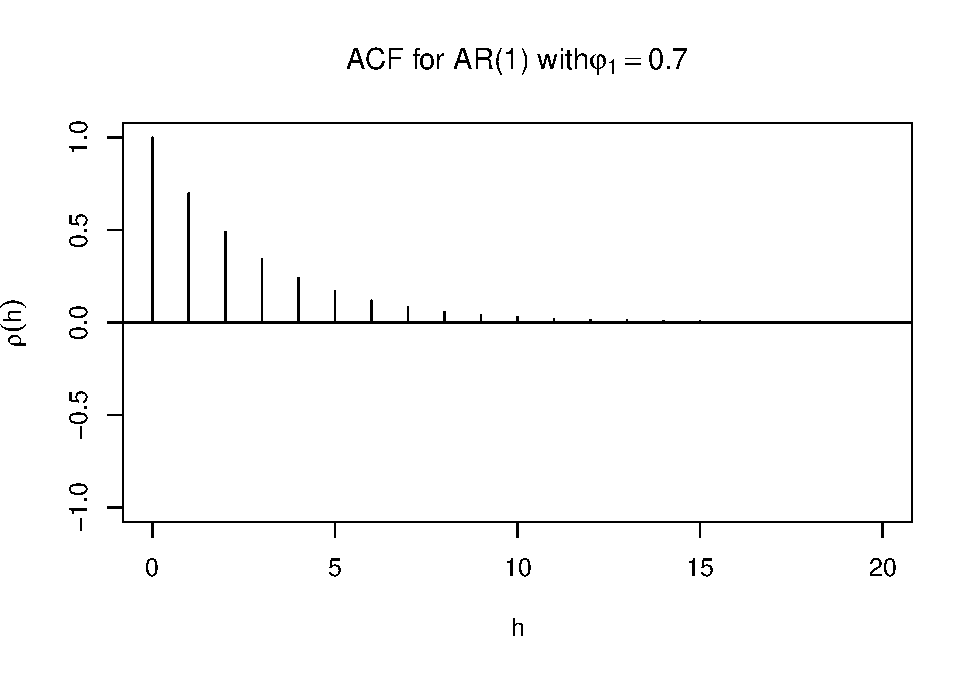
\includegraphics{04-Dependence_files/figure-latex/unnamed-chunk-4-1.pdf}

\begin{Shaded}
\begin{Highlighting}[]
\FunctionTok{cor}\NormalTok{(}\AttributeTok{x =}\NormalTok{ x[}\DecValTok{3}\SpecialCharTok{:}\DecValTok{100}\NormalTok{], }\AttributeTok{y =}\NormalTok{ x[}\DecValTok{2}\SpecialCharTok{:}\DecValTok{99}\NormalTok{]) }
\end{Highlighting}
\end{Shaded}

\begin{verbatim}
## [1] -0.1053843
\end{verbatim}

\begin{Shaded}
\begin{Highlighting}[]
\FunctionTok{cor.test}\NormalTok{(}\AttributeTok{x =}\NormalTok{ x[}\DecValTok{3}\SpecialCharTok{:}\DecValTok{100}\NormalTok{], }\AttributeTok{y =}\NormalTok{ x[}\DecValTok{2}\SpecialCharTok{:}\DecValTok{99}\NormalTok{]) }\CommentTok{\#Not significant }
\end{Highlighting}
\end{Shaded}

\begin{verbatim}
## 
##  Pearson's product-moment correlation
## 
## data:  x[3:100] and x[2:99]
## t = -1.0383, df = 96, p-value = 0.3017
## alternative hypothesis: true correlation is not equal to 0
## 95 percent confidence interval:
##  -0.29758249  0.09502345
## sample estimates:
##        cor 
## -0.1053843
\end{verbatim}

Plot 1. is the least choppy (jagged) and plot 2. is the most choppy. Remember what a correlation means.

A positive correlation means that ``large'' values tend to occur with other ``large'' values and ``small'' values tend to occur with other ``small'' values.

A negative correlation means that ``large'' values tend to occur with other ``small'' values and ``small'' values tend to occur with other ``large'' values.

\hypertarget{stationarity}{%
\chapter{Stationarity}\label{stationarity}}

\hypertarget{stationarity-1}{%
\section{Stationarity}\label{stationarity-1}}

Stationarity is a VERY important concept to understand because it allow us to construct time series models.

\begin{definition}
\textbf{Strictly Stationary}

The probabilistic behavior of \(X_{t_1},...,X_{t_k}\) is exactly the same as that of the shifted set \(X_{t_{1+h}},...,X_{t_{k+h}}\) for ANY collection of time points t1,\ldots, tk, for ANY k = 1, 2, \ldots, and for ANY shift h = 0, \(\pm\) 1, \(\pm\) 2, \ldots{} .

Let \(c_1,…, c_k\) be constants. Then\[P(X_{t_1}\leq{c_1},...,X_{t_k}\leq{c_k})=P(X_{t_{1+h}}\leq{c_{1}},...,X_{t_{k+h}}\leq{c_k})\]

i.e., the probability distribution is INVARIANT to time shifts.
\end{definition}

e.g.~\(P(X_1\leq{c_1}, X_2\leq{c_2})=P(X_{10}\leq{c_1}, X_{11}\leq{c_2})\)

Requiring a time series to be strictly stationary is VERY restrictive! A less restrictive requirement is weakly stationary.

\begin{definition}
\textbf{Weakly Stationary}

The first two moments (mean and covariance) of the time series are invariant to time shifts. \[E(X_t)=\mu, \forall t\] and \[ \gamma(t,t+h)=\gamma(0,h), \forall t\]
\end{definition}

Notes:

\begin{itemize}
\item
  \(\mu\) and \(\gamma(0,h)\) are NOT functions of t.\\
\item
  h is the lag\\
\item
  \(\gamma(t, t+h)\) = \(\gamma(0,h)\) for ALL time t means that the autocovariance function ONLY depends on the number of lags of the time shift. Thus,\(\gamma(0,h) = \gamma(1, h+1) = \gamma(2, 2+h) = \gamma(3, 3+h) = …\)
\item
  Because we will generally be dealing with a weakly stationary time series, we can make the following notational change: \(\gamma(h)=\gamma(0,h)=\gamma(t, t+h).\)\\
\item
  The variance of \(X_t\) is \(\gamma(0)\).
\item
  The same notational change can be made to the autocorrelation function (ACF). Thus, \(\rho(h)\) denotes the ACF at lag h. Note that\[\rho(h)=\rho(t,t+h)=\frac{\gamma(t,t+h)}{\sqrt{\gamma(t,t)}\sqrt{\gamma(t+h,t+h)}}=\frac{\gamma(h)}{\sqrt{\gamma(0)}\sqrt{\gamma(0)}}=\frac{\gamma(h)}{\gamma(0)}\]
\item
  Strictly stationary implies weakly stationary, but the reverse is not necessarily true.\\
\item
  Frequently, we will just say ``stationary'' to refer to weakly stationary and say the full ``strictly stationary'' to refer to strictly stationary.
\end{itemize}

\begin{example}
\textbf{White Noise}
Suppose \(w_t \sim ind. N(0,\sigma^2_w ), t=1,…,n.\) Is this a weakly stationary time series?

Yes -- mean is 0 for all wt, variance is constant for all wt, and the covariance is 0 because the random variables are independent. AND, it is also strictly stationary.
\end{example}

\begin{example}
\textbf{Moving Average}

Let \(m_t=\frac{w_t+w_{t-1}+w_{t-2}}{3}, w_t \sim ind. N(0,1 ), t=1,…,n\)

Previously, we found that \(\mu_t=0, \forall t\) and

\[\begin{cases}
  \gamma(s,t)= \frac{3}{9} & \text{if } s=t \\
  \gamma(s,t)= \frac{2}{9} & \text{if } |s-t|=1\\
  \gamma(s,t)= \frac{1}{9} & \text{if } |s-t|=2\\
  \gamma(s,t)= 0 & \text{if } |s-t|\ge 3\\
\end{cases}\]

Is the time series weakly stationary? Hint: let h=s-t.

Yes! You can see that \(\gamma(s,t)\) only depends on h.
\end{example}

Comments:

\begin{itemize}
\tightlist
\item
  \(\gamma(h) = \gamma(-h)\) for all h if the series is weakly stationary. This means that it does not matter which way the shift occurs.\\
\item
  Stationarity can also be examined when two time series are of interest. We will examine this in more detail later in the course.
\end{itemize}

In summary,

\begin{itemize}
\tightlist
\item
  Both time series must have constant mean
\item
  Both autocovariance functions must depend only on the lag difference
\item
  The ``cross-covariance'' function, the extension of the autocovariance function for one time series to two time series, must depend only on the lag difference. The cross-covariance function is defined as
\end{itemize}

\[\gamma_{xy}(h) = E[(x_{t+h} – \mu_x)(y_t – \mu_y)]\]

Note that \(\gamma_{xy}(h)\) is not necessarily equal to \(\gamma_{yx}(h)\) (usually will be different).

\begin{example}
Let \(x_t = w_t + w_{t-1}\) and \(y_t = w_t - w_{t-1}\), where \(w_t \sim \mathrm{ind}N(0,\sigma^2_w )\) for t = 1, \ldots, n

Claim: \(x_t\) and \(y_t\) are weakly stationary.
\end{example}

\begin{proof}
\leavevmode

\begin{itemize}
\tightlist
\item
  \(X_t\)
\end{itemize}

\(E(X_t)=E(w_t+w_{t-1})=E(w_t+w_{t-1})=0+0=0\)
Thus \(E(X_t)=\mu_{X_t}=0 \forall t\)

\(\gamma(s,t)=E[(X_s-\mu_{X_s})(X_t-\mu_{X_t})]\\=E[X_sX_t]=E[(w_s+w_{s+1})(w_t+w_{t+1})]\\=E[w_sw_t+w_{s-1}w_t+w_sw_{t-1}+w_{s-1}w_{t-1}]\)

if s=t, then \(\gamma(t,t)=E[w^2_t+ w_{t-1}w_t + w_tw_{t-1} + w^2_{t-1}]\\= Var(w_t) + (E[w_t])^2 + 2E[w_{t-1}]E[w_t] + Var(w_{t-1}) + (E[w_{t-1}])^2\\= \sigma^2_w + 0 + 0 + \sigma^2_w + 0= 2\sigma^2_w\)

if s=t-1, then \(\gamma(t-1,t)=E[w_{t-1}w_t+ w_{t-2}w_t + w^2_{t-1} + w_{t-2}w_{t-1}]\\= E[w_{t-1}]E[w_t] + E[w_{t-2}]E[w_t] + Var(w_{t-1}) +(E[w_{t-1}])^2 + E[w_{t-2}]E[w_{t-1}]\\= 0 + 0 + \sigma^2_w + 0+0=\sigma^2_w\)

Note that \(\gamma(t - 1, t) = \sigma^2_w\) and \(\gamma(s,t) = 0\) for \textbar s - t\textbar\textgreater1.

\[\begin{cases}
  \gamma(s,t)= 2\sigma^2_w & \text{if } s=t \\
  \gamma(s,t)= \sigma^2_w & \text{if } |s-t|=1\\
  \gamma(s,t)= 0 & \text{if } |s-t| > 1\\
\end{cases}\]

\(X_t\) is weakly stationary.

\begin{itemize}
\tightlist
\item
  \(Y_t\)
\end{itemize}

\(E(Y_t)=E(w_t-w_{t-1})=E(w_t-w_{t-1})=0-0=0\)
Thus \(E(Y_t)=\mu_{Y_t}=0 \forall t\)

\(\gamma(s,t)=E[(Y_s-\mu_{Y_s})(Y_t-\mu_{Y_t})]=E[Y_sY_t]\\=E[(w_s-w_{s+1})(w_t-w_{t+1})]=\\E[w_sw_t-w_{s-1}w_t-w_sw_{t-1}+w_{s-1}w_{t-1}]\)

if s=t, then \(\gamma(t,t)=E[w^2_t- w_{t-1}w_t - w_tw_{t-1} + w^2_{t-1}]\\= Var(w_t) + (E[w_t])^2 - 2E[w_{t-1}]E[w_t] + Var(w_{t-1}) + (E[w_{t-1}])^2\\= \sigma^2_w + 0 - 0 + \sigma^2_w + 0= 2\sigma^2_w\)

if s=t-1, then \(\gamma(t-1,t)=E[w_{t-1}w_t- w_{t-2}w_t - w^2_{t-1} + w_{t-2}w_{t-1}]\\ = E[w_{t-1}]E[w_t] - E[w_{t-2}]E[w_t] - Var(w_{t-1}) -(E[w_{t-1}])^2 + E[w_{t-2}]E[w_{t-1}]\\= 0 - 0 - \sigma^2_w - 0+0=-\sigma^2_w\)

Note that \(\gamma(t - 1, t) = -\sigma^2_w\) and \(\gamma(s,t) = 0\) for \textbar s - t\textbar\textgreater1.

\[\begin{cases}
  \gamma(s,t)= 2\sigma^2_w & \text{if } s=t \\
  \gamma(s,t)= -\sigma^2_w & \text{if } |s-t|=1\\
  \gamma(s,t)= 0 & \text{if } |s-t| > 1\\
\end{cases}\]

\(Y_t\) is weakly stationary.

\end{proof}

\hypertarget{linear-process}{%
\section{Linear Process}\label{linear-process}}

The previous examples are special cases of a ``linear process''. In general, a linear process can be defined as \[X_t=\mu+ \sum_{j=-\infty}^{\infty} \psi_jw_{t-j}, \sum_{j=-\infty}^{\infty}|\psi_j|<\infty\] and \[w_t\sim\mathrm{ind.}N(0,\sigma^2_w)\]

It can be shown that \(\gamma(h)=\sigma^2_w\sum_{j=-\infty}^{\infty}\psi_{j+h}\psi_j\) for h \(\geq\) 0 provided the series is stationary (remember that and \(\gamma(h) = \gamma(-h)\)).

\begin{proof}
WLOG, let \(\mu=0\), since constants do not affect a covariance.

\(E(X_t)=E(\mu+\sum_{j=-\infty}^{\infty} \psi_jw_{t-j})\\=0+\sum_{j=-\infty}^{\infty} \psi_jE(w_{t-j})\\=0+\sum_{j=-\infty}^{\infty} \psi_j0=0\)

Note that \(\gamma(h) = Cov(x_t, x_{t+h}) = E(x_tx_{t+h}) – E(x_t)E(x_{t+h}) = E(x_tx_{t+h})\) since \(E(x_t) = E(x_{t+h}) = 0\)

Then \(E(x_tx_{t+h})=E[(\sum_{i=-\infty}^{\infty}\psi_iw_{t-i})(\sum_{i=-\infty}^{\infty}\psi_jw_{t+h-j})]\\=E[\sum_{i=-\infty}^{\infty}\sum_{j=-\infty}^{\infty}\psi_i\psi_jw_{t-i}w_{t+h-j}]\\=\sum_{i=-\infty}^{\infty}\sum_{j=-\infty}^{\infty}\psi_i\psi_jE(w_{t-i}w_{t+h-j})\\=\sigma^2_w\sum_{k=-\infty}^{\infty}\psi_k\psi_{k+h}\)

Note that \(E(w_{t-i}w_{t+h-j})=0, \forall -i\ne{h-j}\) and \(E(w_{t-i}w_{t+h-j})=E(w^2_{t-i})=\sigma^2_w ,\forall -i=h-j ( i.e.,j-i=h)\) and \(\psi's\) are constants.

Hence, \(\gamma(h)=\sigma^2_w\sum_{j=-\infty}^{\infty}\psi_{j+h}\psi_j\) for h \(\geq\) 0.
\end{proof}

Important:

There is a very important case when weakly stationary implies strictly stationary. This occurs when the time series has a multivariate normal distribution. Remember that a univariate normal distribution is defined only by its mean and variance. The multivariate normal distribution is defined only by its mean vector and covariance matrix.

Thus, if we can assume a multivariate normal distribution, we ONLY need to check if the time series satisfies the weakly stationary requirements to say the time series is strongly stationary. Thus, notice what the word ``stationary'' would mean in this case.

\begin{example}
\textbf{Visualizing Stationarity}

Below are a few plots of the observed values of a time series. Identify which plots correspond to a weakly stationary series.

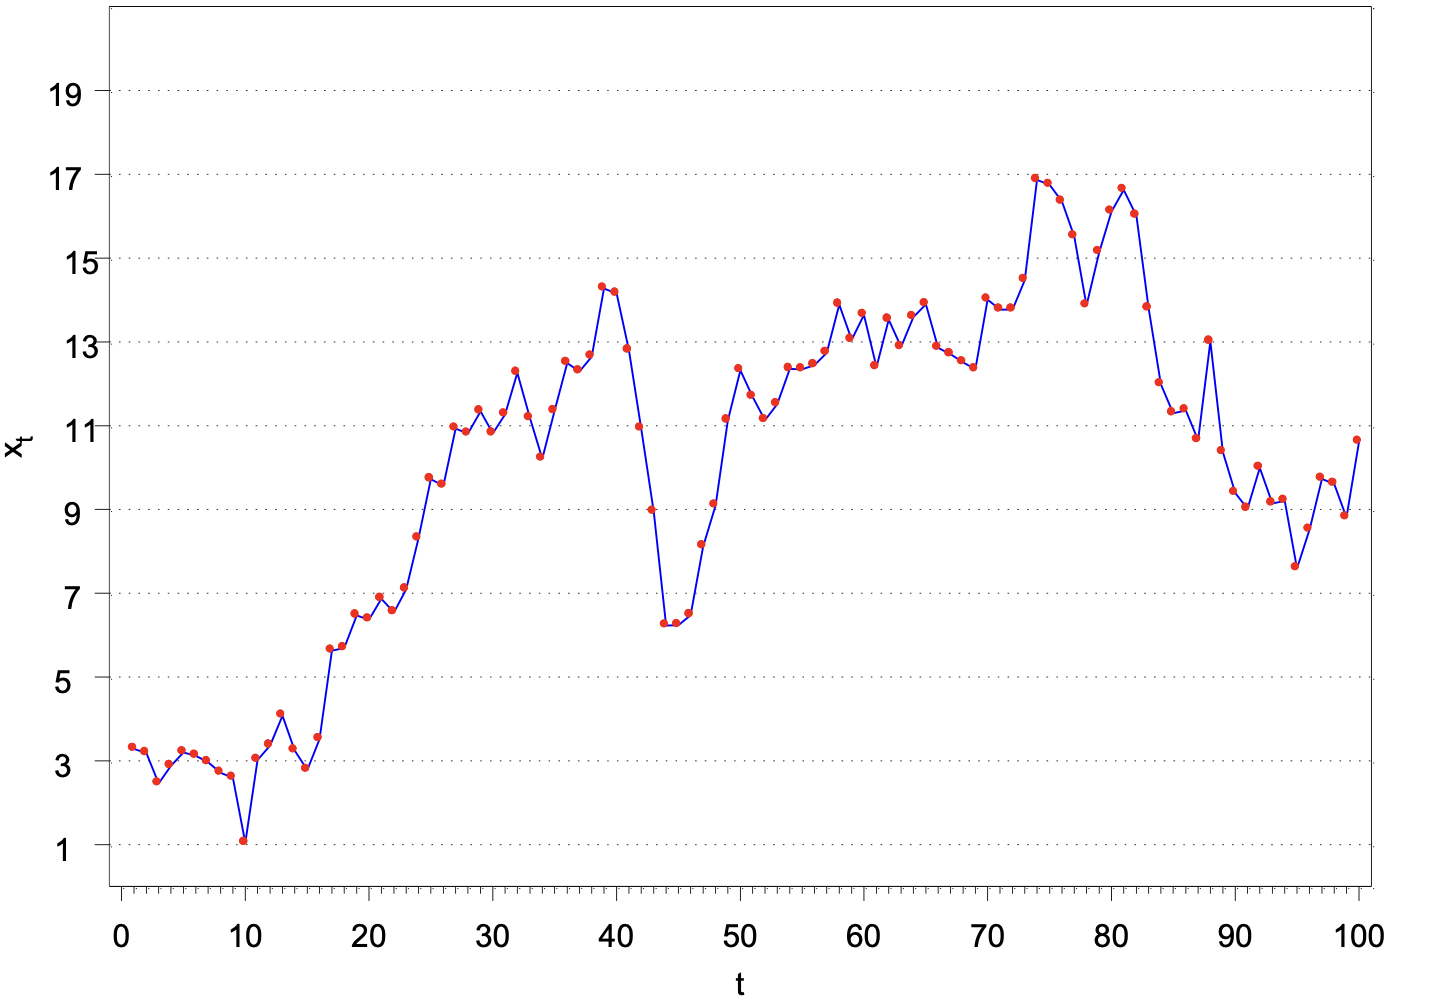
\includegraphics{Stationarity-graph1.png}
This graph violates weakly stationary. It seems that there's a structural change. You can find there are two distinct mean: high mean and low mean.

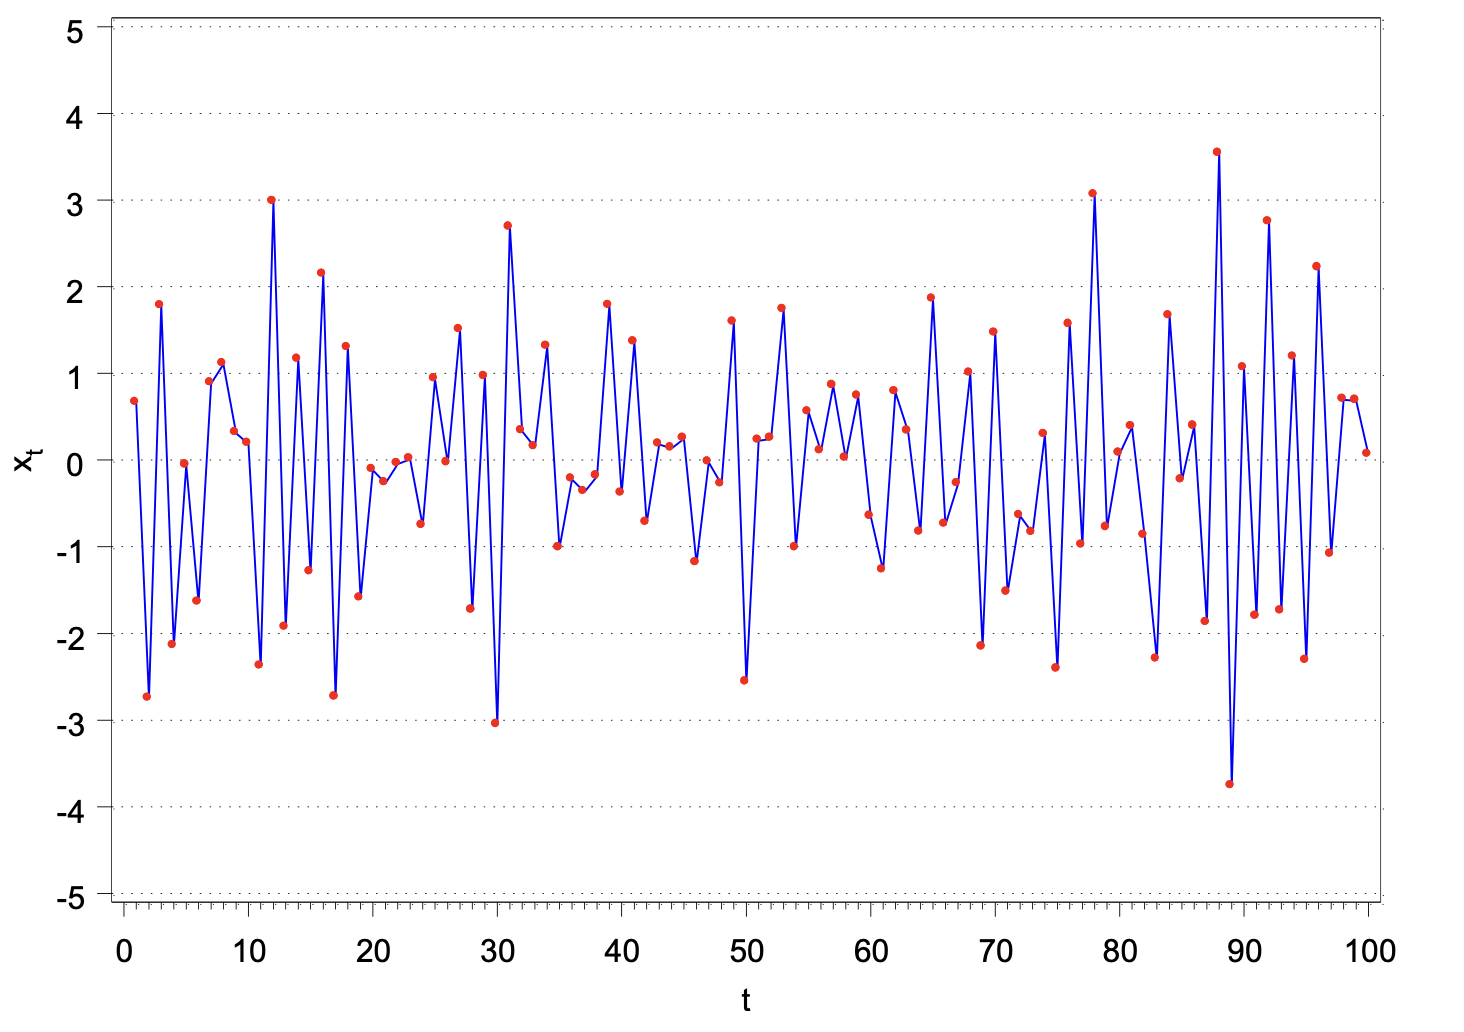
\includegraphics{Stationarity-graph2.png}
This graph doesn't seem to violate weakly stationary, as you can see the mean seems to be a constant 0 and the variablity seems to be a constant across different time points.

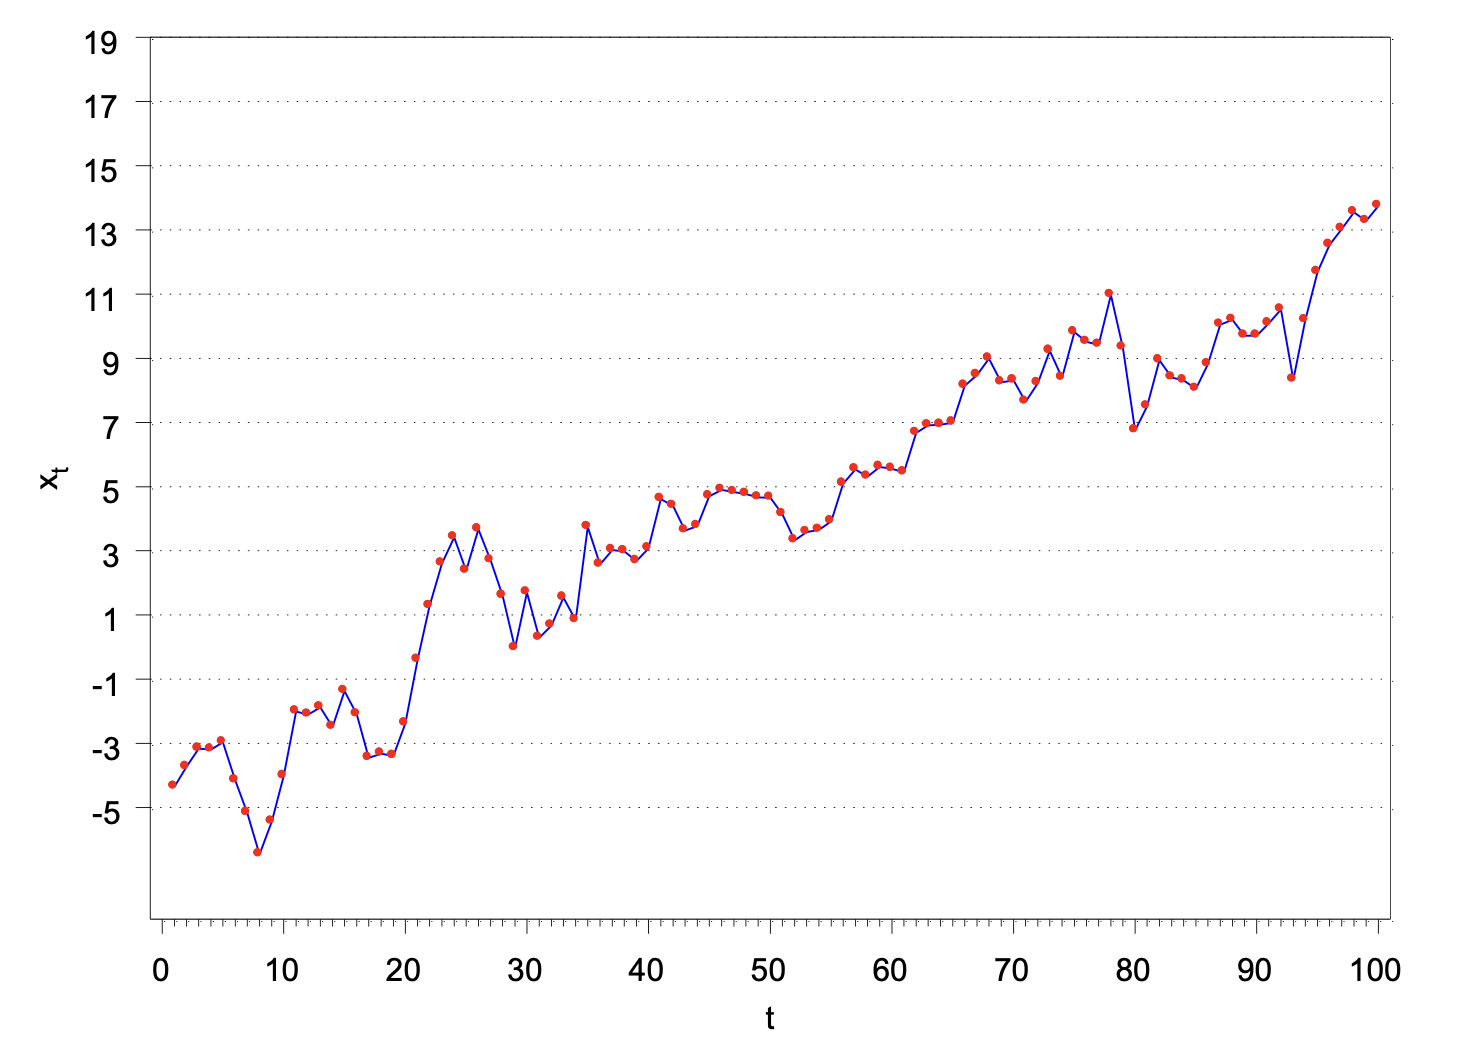
\includegraphics{Stationarity-graph3.png}
Clearly, this violates weakly stationary. You can see the mean keeps changing.

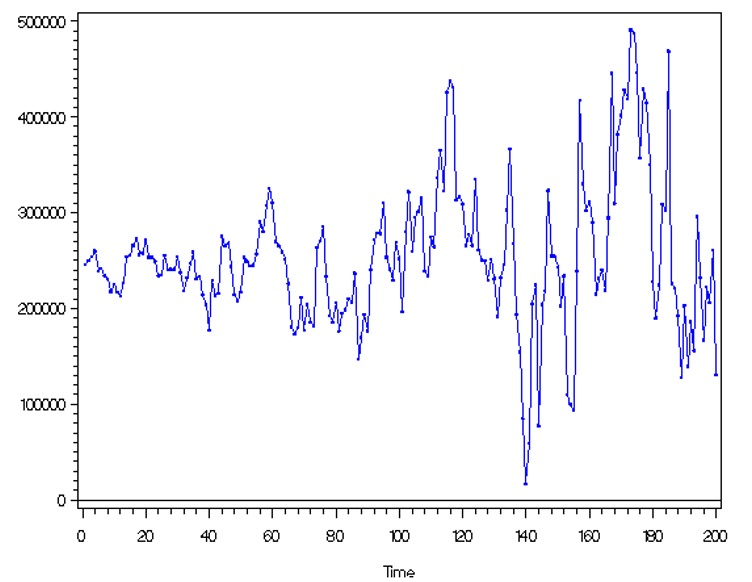
\includegraphics{Stationarity-graph4.jpg}
Clearly, this violates weakly stationary. You can see the variance keeps changing.
\end{example}

It is important to have stationarity b/c it allows us to estimate the mean and variance and we need consistency to construct a model.

\hypertarget{estimation-and-inference-for-measures-of-dependence}{%
\chapter{Estimation and Inference for measures of dependence}\label{estimation-and-inference-for-measures-of-dependence}}

\(\mu, \gamma(h),\rho(h)\) are usually unknown so we need to estimate them. To estimate these quantities, we need to assume the time series is weakly stationary.

\hypertarget{sample-mean-function}{%
\section{Sample mean function}\label{sample-mean-function}}

By the weakly stationary assumption, \(E(x_1) = \mu, E(x_2) = \mu,…, E(x_n) = \mu\). Thus, a logical estimate of \(\mu\) is\[\bar{X}=\frac{1}{n}\sum_{t=1}^{n}X_t\]
Note that this would not make sense to do if the weakly stationarity assumption did not hold!

\hypertarget{sample-autocovariance-function}{%
\section{Sample autocovariance function}\label{sample-autocovariance-function}}

Again with the weakly stationarity assumption, we only need to worry about the lag difference. The estimated autocovariance function is: \[\hat{\gamma}(h)=\frac{1}{n}\sum_{t=1}^{n-h}(X_{t+h}-\bar{X})(X_t-\bar{X})\]

\begin{itemize}
\tightlist
\item
  \(\hat{\gamma}(h)=\hat{\gamma}(-h)\)
\item
  What is this quantity if h = 0?

  \begin{itemize}
  \tightlist
  \item
    \(\hat{\gamma}(h)=\frac{1}{n}\sum_{t=1}^{n}(X_t-\bar{X})(X_t-\bar{X})\), which is essentially the sample variance.(when n is large n\(\approx\)n-1)
  \end{itemize}
\item
  What is this quantity if h =1?

  \begin{itemize}
  \tightlist
  \item
    \(\hat{\gamma}(h)=\frac{1}{n}\sum_{t=1}^{n-1}(X_{t+1}-\bar{X})(X_t-\bar{X})\)
  \end{itemize}
\item
  This is similar to the formula often used to estimate the covariance between two random variables x and y: \(\hat{Cov}(X,Y)=\frac{1}{n}\sum_{i=1}^{n}(X_i-\bar{X})(Y_i-\bar{Y})\).
\item
  The sum goes up to n - h to avoid having negative subscripts in the x's.
\item
  This is NOT an unbiased estimate of \(\gamma(h)\)! However, as n gets larger, the bias will go to 0.
\end{itemize}

\hypertarget{sample-autocorrelation-function-acf}{%
\section{Sample autocorrelation function (ACF)}\label{sample-autocorrelation-function-acf}}

\[\hat{\rho}(h)=\frac{\hat{\gamma}(h)}{\hat{\gamma}(0)}\]

Question: What does \(\rho(h) = 0\) mean and why would this be important to detect?

That means there's no linear relationship between \(X_{t-h}\) and \(X_t\) for this particular lag h. This is important b/c this makes it no sense to use \(X_{t-h}\) to predict \(X_t\).

Because this is important, we conduct hypothesis tests for \(\rho(h)\) for all h \(\ne\) 0! To do the hypothesis test, we need to find the sampling distribution for \(\hat{\rho}(h)\) under the null hypothesis of \(\rho(h)\) = 0.

\hypertarget{sampling-distribution}{%
\section{Sampling distribution}\label{sampling-distribution}}

In summary, if \(\rho(h)\) = 0, \(x_t\) is stationary, and the sample size is ``large'', then \(\hat{\rho}(h)\) has an approximate normal distribution with mean 0 and standard deviation \(\sigma_{\hat{\rho}(h)}=\frac{1}{\sqrt{n}}\), i.e., \(\hat{\rho}(h)\sim N(0,\frac{1}{\sqrt{n}})\)

A proof is available in Shumway and Stoffer's textbook and requires an understanding asymptotics (PhD level statistics course). (\(\sqrt{n}(\hat{\rho}(h)-0) \to^{d} N(0,1)\))

\(H_0: \rho(h)=0\)

\(Z=\frac{\hat{\rho}(h)-0}{\frac{1}{\sqrt{n}}}\)

\(Z>|Z_{1-\frac{\alpha}{2}}|\) reject \(H_0\)

\(\hat{\rho}(h)>\pm \frac{Z_{1-\frac{\alpha}{2}}}{\sqrt{n}}\) reject \(H_0\)

For a hypothesis test, we could check if \(\hat{\rho}(h)\) is within the bounds of 0 \(\pm \frac{Z_{1-\frac{\alpha}{2}}}{\sqrt{n}}\) or not where P(Z \textless{} \(Z_{1-\frac{\alpha}{2}}\)) = 1 -- \(\frac{\alpha}{2}\) for a standard normal random variable Z. If it is not, then there is sufficient evidence to conclude that \(\rho(h) \ne\) 0. We will be using this result a lot for the rest of this course!

\begin{example}

\(x_t=0.7x_{t-1}+w_t, w_t\sim\mathrm{ind.}N(0,1), n=100\)

Click \href{http://www.chrisbilder.com/stat878/sections/2/AR1.0.7.txt}{here} to download data.

\begin{Shaded}
\begin{Highlighting}[]
\NormalTok{ar1 }\OtherTok{\textless{}{-}} \FunctionTok{read.table}\NormalTok{(}\AttributeTok{file =} \StringTok{"AR1.0.7.txt"}\NormalTok{, }\AttributeTok{header =} \ConstantTok{TRUE}\NormalTok{, }\AttributeTok{sep =} \StringTok{""}\NormalTok{)}

\FunctionTok{head}\NormalTok{(ar1)}
\end{Highlighting}
\end{Shaded}

\begin{verbatim}
##   t          x
## 1 1  0.0417268
## 2 2  0.3719068
## 3 3 -0.1854518
## 4 4 -1.3829742
## 5 5 -2.8759365
## 6 6 -2.6001761
\end{verbatim}

\begin{Shaded}
\begin{Highlighting}[]
\NormalTok{x }\OtherTok{\textless{}{-}}\NormalTok{ ar1}\SpecialCharTok{$}\NormalTok{x}
\end{Highlighting}
\end{Shaded}

\begin{Shaded}
\begin{Highlighting}[]
\FunctionTok{dev.new}\NormalTok{(}\AttributeTok{width =} \DecValTok{8}\NormalTok{, }\AttributeTok{height =} \DecValTok{6}\NormalTok{, }\AttributeTok{pointsize =} \DecValTok{10}\NormalTok{)  }
\CommentTok{\#Opens up wider plot window than the default (good for time series plots)}
\FunctionTok{plot}\NormalTok{(}\AttributeTok{x =}\NormalTok{ x, }\AttributeTok{ylab =} \FunctionTok{expression}\NormalTok{(x[t]), }\AttributeTok{xlab =} \StringTok{"t"}\NormalTok{, }\AttributeTok{type =} \StringTok{"l"}\NormalTok{, }\AttributeTok{col =} \StringTok{"red"}\NormalTok{, }\AttributeTok{lwd =} \DecValTok{1}\NormalTok{ , }
     \AttributeTok{main =} \FunctionTok{expression}\NormalTok{(}\FunctionTok{paste}\NormalTok{(}\StringTok{"Data simulated from AR(1): "}\NormalTok{, x[t] }\SpecialCharTok{==} \FloatTok{0.7}\SpecialCharTok{*}\NormalTok{x[t}\DecValTok{{-}1}\NormalTok{] }\SpecialCharTok{+}\NormalTok{ w[t], }\StringTok{" where "}\NormalTok{, w[t], }\StringTok{"\textasciitilde{}N(0,1)"}\NormalTok{)) , }
      \AttributeTok{panel.first=}\FunctionTok{grid}\NormalTok{(}\AttributeTok{col =} \StringTok{"gray"}\NormalTok{, }\AttributeTok{lty =} \StringTok{"dotted"}\NormalTok{))}
\FunctionTok{points}\NormalTok{(}\AttributeTok{x =}\NormalTok{ x, }\AttributeTok{pch =} \DecValTok{20}\NormalTok{, }\AttributeTok{col =} \StringTok{"blue"}\NormalTok{)}
\end{Highlighting}
\end{Shaded}

The easiest way to find the autocorrelations in R is to use the \texttt{acf()} function.

\begin{Shaded}
\begin{Highlighting}[]
\NormalTok{rho.x }\OtherTok{\textless{}{-}} \FunctionTok{acf}\NormalTok{(}\AttributeTok{x =}\NormalTok{ x, }\AttributeTok{type =} \StringTok{"correlation"}\NormalTok{, }\AttributeTok{main =}
             \FunctionTok{expression}\NormalTok{(}\FunctionTok{paste}\NormalTok{(}\StringTok{"Data simulated from AR(1): "}\NormalTok{, x[t] }\SpecialCharTok{==} \FloatTok{0.7}\SpecialCharTok{*}\NormalTok{x[t}\DecValTok{{-}1}\NormalTok{] }\SpecialCharTok{+}\NormalTok{ w[t], }\StringTok{" where "}\NormalTok{, w[t], }\StringTok{"\textasciitilde{}N(0,1)"}\NormalTok{)))}
\end{Highlighting}
\end{Shaded}

\includegraphics{06-Estimation-and-Inference_files/figure-latex/unnamed-chunk-3-1.pdf}

\begin{Shaded}
\begin{Highlighting}[]
  \CommentTok{\# ci argument can be used to change 1 {-} alpha for plot}
  \CommentTok{\# lag.max argument can be used to change the maximum number of lags}
\end{Highlighting}
\end{Shaded}

In our language, the horizontal axis: lag=h, the verical axis: ACF=\(\hat{\rho}(h)\)

The horizontal lines on the plot are drawn at 0 \(\pm \frac{Z_{1-\frac{0.05}{2}}}{\sqrt{n}}\) where \(Z_{1-\frac{0.05}{2}} = 1.96\).
i.e., outside the blue dashed line, we reject \(H_0\)

The location of the lines can be changed by using the \texttt{ci} (confidence interval )argument. The default is ci = 0.95. i.e., \(\alpha=0.05\)

\begin{Shaded}
\begin{Highlighting}[]
\NormalTok{rho.x}
\end{Highlighting}
\end{Shaded}

\begin{verbatim}
## 
## Autocorrelations of series 'x', by lag
## 
##      0      1      2      3      4      5      6      7      8      9     10 
##  1.000  0.674  0.401  0.169 -0.023 -0.125 -0.067 -0.064 -0.058  0.005 -0.044 
##     11     12     13     14     15     16     17     18     19     20 
## -0.041 -0.017  0.064  0.076  0.160  0.191  0.141  0.081  0.006 -0.132
\end{verbatim}

\begin{Shaded}
\begin{Highlighting}[]
\CommentTok{\# the first one is rho\_hat(0)}
\CommentTok{\# the second one is rho\_hat(1)}
\end{Highlighting}
\end{Shaded}

\begin{Shaded}
\begin{Highlighting}[]
\FunctionTok{names}\NormalTok{(rho.x)}
\end{Highlighting}
\end{Shaded}

\begin{verbatim}
## [1] "acf"    "type"   "n.used" "lag"    "series" "snames"
\end{verbatim}

\begin{Shaded}
\begin{Highlighting}[]
\NormalTok{rho.x}\SpecialCharTok{$}\NormalTok{acf}
\end{Highlighting}
\end{Shaded}

\begin{verbatim}
## , , 1
## 
##               [,1]
##  [1,]  1.000000000
##  [2,]  0.673671871
##  [3,]  0.400891188
##  [4,]  0.168552826
##  [5,] -0.023391129
##  [6,] -0.124632501
##  [7,] -0.067392830
##  [8,] -0.064248086
##  [9,] -0.057717749
## [10,]  0.005312358
## [11,] -0.044035976
## [12,] -0.041121407
## [13,] -0.017197132
## [14,]  0.063864970
## [15,]  0.075575696
## [16,]  0.159665692
## [17,]  0.191349965
## [18,]  0.140967540
## [19,]  0.080508273
## [20,]  0.005584061
## [21,] -0.131559629
\end{verbatim}

\begin{Shaded}
\begin{Highlighting}[]
\CommentTok{\# the first one is rho\_hat(0)}
\CommentTok{\# the second one is rho\_hat(1)}
\end{Highlighting}
\end{Shaded}

\begin{Shaded}
\begin{Highlighting}[]
\NormalTok{rho.x}\SpecialCharTok{$}\NormalTok{acf[}\DecValTok{1}\SpecialCharTok{:}\DecValTok{2}\NormalTok{]}
\end{Highlighting}
\end{Shaded}

\begin{verbatim}
## [1] 1.0000000 0.6736719
\end{verbatim}

\end{example}

Questions:

\begin{itemize}
\tightlist
\item
  What happens to the autocorrelations over time? Why do you think this happens?

  \begin{itemize}
  \tightlist
  \item
    From the model \(x_t=0.7x_{t-1}+w_t\), you can see that the auto correlation dies out as the lag term h increases, the main reason is the coefficient 0.7
  \end{itemize}
\item
  Is there a positive or negative correlation?

  \begin{itemize}
  \tightlist
  \item
    A positive correlation, again from our model \(x_t=0.7x_{t-1}+w_t\), 0.7\textgreater0
  \end{itemize}
\item
  At what lags is \$\rho(h)\ne\$0?

  \begin{itemize}
  \tightlist
  \item
    h=0,1,2. But we don't care h=0, it's 1 just by definition.
  \end{itemize}
\end{itemize}

R plots \(\hat{\rho}(0)=1\) by default. This is unnecessary because \(\hat{\rho}(0)\) will be 1 for all time series data sets (again, it's just by definition)! To remove \(\hat{\rho}(0)\) from the plot, one can specify the x-axis limit to start at 1. Below is one way this can be done and also illustrates how to use the \texttt{lag.max} argument.

\begin{Shaded}
\begin{Highlighting}[]
\FunctionTok{par}\NormalTok{(}\AttributeTok{xaxs =} \StringTok{"i"}\NormalTok{) }
\CommentTok{\# Remove default 4\% extra space around  min and max of x{-}axis}

\NormalTok{rho.x2 }\OtherTok{\textless{}{-}} \FunctionTok{acf}\NormalTok{(}\AttributeTok{x =}\NormalTok{ x, }\AttributeTok{type =} \StringTok{"correlation"}\NormalTok{, }\AttributeTok{xlim =} 
    \FunctionTok{c}\NormalTok{(}\DecValTok{0}\NormalTok{,}\DecValTok{30}\NormalTok{), }\AttributeTok{lag.max =} \DecValTok{30}\NormalTok{, }\AttributeTok{main =} \FunctionTok{expression}\NormalTok{(}\FunctionTok{paste}\NormalTok{(}\StringTok{"Data }
\StringTok{    simulated from AR(1): "}\NormalTok{, x[t] }\SpecialCharTok{==} \FloatTok{0.7}\SpecialCharTok{*}\NormalTok{x[t}\DecValTok{{-}1}\NormalTok{] }\SpecialCharTok{+}\NormalTok{ w[t], }\StringTok{" }
\StringTok{    where "}\NormalTok{, w[t], }\StringTok{"\textasciitilde{}N(0,1)"}\NormalTok{)))}
\end{Highlighting}
\end{Shaded}

\begin{verbatim}
## Warning in title(main %||% if (i == j) snames[i] else paste(sn.abbr[i], : font
## metrics unknown for character 0xa

## Warning in title(main %||% if (i == j) snames[i] else paste(sn.abbr[i], : font
## metrics unknown for character 0xa

## Warning in title(main %||% if (i == j) snames[i] else paste(sn.abbr[i], : font
## metrics unknown for character 0xa

## Warning in title(main %||% if (i == j) snames[i] else paste(sn.abbr[i], : font
## metrics unknown for character 0xa
\end{verbatim}

\includegraphics{06-Estimation-and-Inference_files/figure-latex/unnamed-chunk-8-1.pdf}

\begin{Shaded}
\begin{Highlighting}[]
\FunctionTok{par}\NormalTok{(}\AttributeTok{xaxs =} \StringTok{"r"}\NormalTok{) }\CommentTok{\# Return to the default: regular pattern}
\end{Highlighting}
\end{Shaded}

Note that \(\hat{\rho}(0)=1\) is still present but the y-axis at x = 0 hides it.

While displaying \(\hat{\rho}(0)=1\) may seem minor, we will examine these autocorrelations later in the course to determine an appropriate model for a data set. Often, one will forget to ignore the line drawn at lag = 0 and choose an incorrect model.

\textbf{You should always ignore the line drawn at lag=0!!! b/c it's 1 just by definition.}

The autocovariances can also be found using \texttt{acf()}.

\begin{Shaded}
\begin{Highlighting}[]
\FunctionTok{acf}\NormalTok{(}\AttributeTok{x =}\NormalTok{ x, }\AttributeTok{type =} \StringTok{"covariance"}\NormalTok{, }\AttributeTok{main =} 
     \FunctionTok{expression}\NormalTok{(}\FunctionTok{paste}\NormalTok{(}\StringTok{"Data simulated from AR(1): "}\NormalTok{, x[t] }
     \SpecialCharTok{==} \FloatTok{0.7}\SpecialCharTok{*}\NormalTok{x[t}\DecValTok{{-}1}\NormalTok{] }\SpecialCharTok{+}\NormalTok{ w[t], }\StringTok{" where "}\NormalTok{, w[t], }\StringTok{"\textasciitilde{}N(0,1)"}\NormalTok{)))}
\end{Highlighting}
\end{Shaded}

\includegraphics{06-Estimation-and-Inference_files/figure-latex/unnamed-chunk-9-1.pdf}

To help understand autocorrelations and their relationship with the correlation coefficient better, I decided to look at the ``usual'' estimated Pearson correlation coefficients between \(x_t, x_{t-1}, x_{t-2},\) and \(x_{t-3}\).

\begin{Shaded}
\begin{Highlighting}[]
\CommentTok{\# Examine usual ways to check correlation}
\NormalTok{x.ts }\OtherTok{\textless{}{-}} \FunctionTok{ts}\NormalTok{(x)}
\NormalTok{x.ts}
\end{Highlighting}
\end{Shaded}

\begin{verbatim}
## Time Series:
## Start = 1 
## End = 100 
## Frequency = 1 
##   [1]  0.04172680  0.37190682 -0.18545185 -1.38297422 -2.87593652 -2.60017605
##   [7] -1.10401719 -0.46385116  0.80339069  2.11483585  3.39124978  3.86739194
##  [13]  2.12733595  0.67590604  0.71429367  0.38928044 -1.22681923  0.02287443
##  [19] -0.57321924 -2.68376851 -4.80850095 -2.44797633 -1.73921817 -1.48773023
##  [25]  0.68920966  0.40220308 -1.58781041 -2.07300848 -2.63408197 -3.54333559
##  [31] -2.74116328 -2.54401750 -3.19570817 -0.02623669  0.41663974 -1.74485791
##  [37] -3.04847994 -1.64692948 -1.71478199  0.11340965  1.55017869  0.47317192
##  [43] -0.18521791 -0.05759091 -1.32105323 -1.22071881 -1.53827085  0.01277076
##  [49] -3.19955388 -3.11022833 -3.30621969 -2.00546537  0.18084415  0.58776479
##  [55] -0.70238414 -0.34570939  0.94209248 -0.78176791  1.30547320 -1.04054783
##  [61] -1.06897160 -1.08850000  0.06031172 -0.05724856 -1.14731083 -0.79262221
##  [67] -0.55565451 -1.55985750 -2.17062644 -1.07776017  0.51569067  2.30660050
##  [73]  1.53530426  2.55899301  1.83836277  1.08072014  1.34125182 -0.80729300
##  [79] -1.42735924 -0.42456207 -0.11625003 -0.74807460  0.70052717  0.08557377
##  [85] -0.06039041  0.04479407 -0.12657328 -1.30097021  0.81586192 -0.13139757
##  [91]  1.84725644  1.62364752  0.33080663 -0.40824385 -1.56008530 -1.63175408
##  [97] -1.36418639 -0.37209392 -0.65833401  2.03705932
\end{verbatim}

\begin{Shaded}
\begin{Highlighting}[]
\NormalTok{set1 }\OtherTok{\textless{}{-}} \FunctionTok{ts.intersect}\NormalTok{(x.ts, }\AttributeTok{x.ts1 =} \FunctionTok{lag}\NormalTok{(}\AttributeTok{x =}\NormalTok{ x.ts, }\AttributeTok{k =} \SpecialCharTok{{-}}\DecValTok{1}\NormalTok{), }\AttributeTok{x.ts2 =} \FunctionTok{lag}\NormalTok{(}\AttributeTok{x =}\NormalTok{ x.ts, }\AttributeTok{k =} \SpecialCharTok{{-}}\DecValTok{2}\NormalTok{), }\AttributeTok{x.ts3 =} \FunctionTok{lag}\NormalTok{(}\AttributeTok{x =}\NormalTok{ x.ts, }\AttributeTok{k =} \SpecialCharTok{{-}}\DecValTok{3}\NormalTok{))}

\CommentTok{\# b/c we use ts.intersect (take intersection), we have the following}
\CommentTok{\# x.ts starts at X4}
\CommentTok{\# x.ts1 starts at X3}
\CommentTok{\# x.ts2 starts at X2}
\CommentTok{\# x.ts3 starts at X1}
  
\NormalTok{set1}
\end{Highlighting}
\end{Shaded}

\begin{verbatim}
## Time Series:
## Start = 4 
## End = 100 
## Frequency = 1 
##            x.ts       x.ts1       x.ts2       x.ts3
##   4 -1.38297422 -0.18545185  0.37190682  0.04172680
##   5 -2.87593652 -1.38297422 -0.18545185  0.37190682
##   6 -2.60017605 -2.87593652 -1.38297422 -0.18545185
##   7 -1.10401719 -2.60017605 -2.87593652 -1.38297422
##   8 -0.46385116 -1.10401719 -2.60017605 -2.87593652
##   9  0.80339069 -0.46385116 -1.10401719 -2.60017605
##  10  2.11483585  0.80339069 -0.46385116 -1.10401719
##  11  3.39124978  2.11483585  0.80339069 -0.46385116
##  12  3.86739194  3.39124978  2.11483585  0.80339069
##  13  2.12733595  3.86739194  3.39124978  2.11483585
##  14  0.67590604  2.12733595  3.86739194  3.39124978
##  15  0.71429367  0.67590604  2.12733595  3.86739194
##  16  0.38928044  0.71429367  0.67590604  2.12733595
##  17 -1.22681923  0.38928044  0.71429367  0.67590604
##  18  0.02287443 -1.22681923  0.38928044  0.71429367
##  19 -0.57321924  0.02287443 -1.22681923  0.38928044
##  20 -2.68376851 -0.57321924  0.02287443 -1.22681923
##  21 -4.80850095 -2.68376851 -0.57321924  0.02287443
##  22 -2.44797633 -4.80850095 -2.68376851 -0.57321924
##  23 -1.73921817 -2.44797633 -4.80850095 -2.68376851
##  24 -1.48773023 -1.73921817 -2.44797633 -4.80850095
##  25  0.68920966 -1.48773023 -1.73921817 -2.44797633
##  26  0.40220308  0.68920966 -1.48773023 -1.73921817
##  27 -1.58781041  0.40220308  0.68920966 -1.48773023
##  28 -2.07300848 -1.58781041  0.40220308  0.68920966
##  29 -2.63408197 -2.07300848 -1.58781041  0.40220308
##  30 -3.54333559 -2.63408197 -2.07300848 -1.58781041
##  31 -2.74116328 -3.54333559 -2.63408197 -2.07300848
##  32 -2.54401750 -2.74116328 -3.54333559 -2.63408197
##  33 -3.19570817 -2.54401750 -2.74116328 -3.54333559
##  34 -0.02623669 -3.19570817 -2.54401750 -2.74116328
##  35  0.41663974 -0.02623669 -3.19570817 -2.54401750
##  36 -1.74485791  0.41663974 -0.02623669 -3.19570817
##  37 -3.04847994 -1.74485791  0.41663974 -0.02623669
##  38 -1.64692948 -3.04847994 -1.74485791  0.41663974
##  39 -1.71478199 -1.64692948 -3.04847994 -1.74485791
##  40  0.11340965 -1.71478199 -1.64692948 -3.04847994
##  41  1.55017869  0.11340965 -1.71478199 -1.64692948
##  42  0.47317192  1.55017869  0.11340965 -1.71478199
##  43 -0.18521791  0.47317192  1.55017869  0.11340965
##  44 -0.05759091 -0.18521791  0.47317192  1.55017869
##  45 -1.32105323 -0.05759091 -0.18521791  0.47317192
##  46 -1.22071881 -1.32105323 -0.05759091 -0.18521791
##  47 -1.53827085 -1.22071881 -1.32105323 -0.05759091
##  48  0.01277076 -1.53827085 -1.22071881 -1.32105323
##  49 -3.19955388  0.01277076 -1.53827085 -1.22071881
##  50 -3.11022833 -3.19955388  0.01277076 -1.53827085
##  51 -3.30621969 -3.11022833 -3.19955388  0.01277076
##  52 -2.00546537 -3.30621969 -3.11022833 -3.19955388
##  53  0.18084415 -2.00546537 -3.30621969 -3.11022833
##  54  0.58776479  0.18084415 -2.00546537 -3.30621969
##  55 -0.70238414  0.58776479  0.18084415 -2.00546537
##  56 -0.34570939 -0.70238414  0.58776479  0.18084415
##  57  0.94209248 -0.34570939 -0.70238414  0.58776479
##  58 -0.78176791  0.94209248 -0.34570939 -0.70238414
##  59  1.30547320 -0.78176791  0.94209248 -0.34570939
##  60 -1.04054783  1.30547320 -0.78176791  0.94209248
##  61 -1.06897160 -1.04054783  1.30547320 -0.78176791
##  62 -1.08850000 -1.06897160 -1.04054783  1.30547320
##  63  0.06031172 -1.08850000 -1.06897160 -1.04054783
##  64 -0.05724856  0.06031172 -1.08850000 -1.06897160
##  65 -1.14731083 -0.05724856  0.06031172 -1.08850000
##  66 -0.79262221 -1.14731083 -0.05724856  0.06031172
##  67 -0.55565451 -0.79262221 -1.14731083 -0.05724856
##  68 -1.55985750 -0.55565451 -0.79262221 -1.14731083
##  69 -2.17062644 -1.55985750 -0.55565451 -0.79262221
##  70 -1.07776017 -2.17062644 -1.55985750 -0.55565451
##  71  0.51569067 -1.07776017 -2.17062644 -1.55985750
##  72  2.30660050  0.51569067 -1.07776017 -2.17062644
##  73  1.53530426  2.30660050  0.51569067 -1.07776017
##  74  2.55899301  1.53530426  2.30660050  0.51569067
##  75  1.83836277  2.55899301  1.53530426  2.30660050
##  76  1.08072014  1.83836277  2.55899301  1.53530426
##  77  1.34125182  1.08072014  1.83836277  2.55899301
##  78 -0.80729300  1.34125182  1.08072014  1.83836277
##  79 -1.42735924 -0.80729300  1.34125182  1.08072014
##  80 -0.42456207 -1.42735924 -0.80729300  1.34125182
##  81 -0.11625003 -0.42456207 -1.42735924 -0.80729300
##  82 -0.74807460 -0.11625003 -0.42456207 -1.42735924
##  83  0.70052717 -0.74807460 -0.11625003 -0.42456207
##  84  0.08557377  0.70052717 -0.74807460 -0.11625003
##  85 -0.06039041  0.08557377  0.70052717 -0.74807460
##  86  0.04479407 -0.06039041  0.08557377  0.70052717
##  87 -0.12657328  0.04479407 -0.06039041  0.08557377
##  88 -1.30097021 -0.12657328  0.04479407 -0.06039041
##  89  0.81586192 -1.30097021 -0.12657328  0.04479407
##  90 -0.13139757  0.81586192 -1.30097021 -0.12657328
##  91  1.84725644 -0.13139757  0.81586192 -1.30097021
##  92  1.62364752  1.84725644 -0.13139757  0.81586192
##  93  0.33080663  1.62364752  1.84725644 -0.13139757
##  94 -0.40824385  0.33080663  1.62364752  1.84725644
##  95 -1.56008530 -0.40824385  0.33080663  1.62364752
##  96 -1.63175408 -1.56008530 -0.40824385  0.33080663
##  97 -1.36418639 -1.63175408 -1.56008530 -0.40824385
##  98 -0.37209392 -1.36418639 -1.63175408 -1.56008530
##  99 -0.65833401 -0.37209392 -1.36418639 -1.63175408
## 100  2.03705932 -0.65833401 -0.37209392 -1.36418639
\end{verbatim}

\begin{Shaded}
\begin{Highlighting}[]
\FunctionTok{cor}\NormalTok{(set1)}
\end{Highlighting}
\end{Shaded}

\begin{verbatim}
##            x.ts     x.ts1     x.ts2     x.ts3
## x.ts  1.0000000 0.6824913 0.4065326 0.1710145
## x.ts1 0.6824913 1.0000000 0.6929638 0.4108375
## x.ts2 0.4065326 0.6929638 1.0000000 0.6935801
## x.ts3 0.1710145 0.4108375 0.6935801 1.0000000
\end{verbatim}

\begin{Shaded}
\begin{Highlighting}[]
\CommentTok{\# corr matrix}
\end{Highlighting}
\end{Shaded}

\begin{Shaded}
\begin{Highlighting}[]
\FunctionTok{library}\NormalTok{(car) }\CommentTok{\#scatterplot.matrix is in this package }
\end{Highlighting}
\end{Shaded}

\begin{verbatim}
## Loading required package: carData
\end{verbatim}

\begin{Shaded}
\begin{Highlighting}[]
\FunctionTok{scatterplotMatrix}\NormalTok{(}\AttributeTok{formula =} \SpecialCharTok{\textasciitilde{}}\NormalTok{x.ts }\SpecialCharTok{+}\NormalTok{ x.ts1 }\SpecialCharTok{+}\NormalTok{ x.ts2 }\SpecialCharTok{+}\NormalTok{ x.ts3, }\AttributeTok{data =}\NormalTok{ set1,}
    \AttributeTok{diagonal =} \FunctionTok{list}\NormalTok{(}\AttributeTok{method =} \StringTok{"histogram"}\NormalTok{), }\AttributeTok{col =} \StringTok{"red"}\NormalTok{)}
\end{Highlighting}
\end{Shaded}

\includegraphics{06-Estimation-and-Inference_files/figure-latex/unnamed-chunk-13-1.pdf}

\begin{Shaded}
\begin{Highlighting}[]
\NormalTok{set2 }\OtherTok{\textless{}{-}} \FunctionTok{ts.intersect}\NormalTok{(x.ts, }\AttributeTok{x.ts1 =} \FunctionTok{lag}\NormalTok{(}\AttributeTok{x =}\NormalTok{ x.ts, }\AttributeTok{k =} \DecValTok{1}\NormalTok{), }\AttributeTok{x.ts2 =} \FunctionTok{lag}\NormalTok{(}\AttributeTok{x =}\NormalTok{ x.ts, }\AttributeTok{k =} \DecValTok{2}\NormalTok{), }\AttributeTok{x.ts3 =} \FunctionTok{lag}\NormalTok{(}\AttributeTok{x =}\NormalTok{ x.ts, }\AttributeTok{k =} \DecValTok{3}\NormalTok{))}

\NormalTok{set2}
\end{Highlighting}
\end{Shaded}

\begin{verbatim}
## Time Series:
## Start = 1 
## End = 97 
## Frequency = 1 
##           x.ts       x.ts1       x.ts2       x.ts3
##  1  0.04172680  0.37190682 -0.18545185 -1.38297422
##  2  0.37190682 -0.18545185 -1.38297422 -2.87593652
##  3 -0.18545185 -1.38297422 -2.87593652 -2.60017605
##  4 -1.38297422 -2.87593652 -2.60017605 -1.10401719
##  5 -2.87593652 -2.60017605 -1.10401719 -0.46385116
##  6 -2.60017605 -1.10401719 -0.46385116  0.80339069
##  7 -1.10401719 -0.46385116  0.80339069  2.11483585
##  8 -0.46385116  0.80339069  2.11483585  3.39124978
##  9  0.80339069  2.11483585  3.39124978  3.86739194
## 10  2.11483585  3.39124978  3.86739194  2.12733595
## 11  3.39124978  3.86739194  2.12733595  0.67590604
## 12  3.86739194  2.12733595  0.67590604  0.71429367
## 13  2.12733595  0.67590604  0.71429367  0.38928044
## 14  0.67590604  0.71429367  0.38928044 -1.22681923
## 15  0.71429367  0.38928044 -1.22681923  0.02287443
## 16  0.38928044 -1.22681923  0.02287443 -0.57321924
## 17 -1.22681923  0.02287443 -0.57321924 -2.68376851
## 18  0.02287443 -0.57321924 -2.68376851 -4.80850095
## 19 -0.57321924 -2.68376851 -4.80850095 -2.44797633
## 20 -2.68376851 -4.80850095 -2.44797633 -1.73921817
## 21 -4.80850095 -2.44797633 -1.73921817 -1.48773023
## 22 -2.44797633 -1.73921817 -1.48773023  0.68920966
## 23 -1.73921817 -1.48773023  0.68920966  0.40220308
## 24 -1.48773023  0.68920966  0.40220308 -1.58781041
## 25  0.68920966  0.40220308 -1.58781041 -2.07300848
## 26  0.40220308 -1.58781041 -2.07300848 -2.63408197
## 27 -1.58781041 -2.07300848 -2.63408197 -3.54333559
## 28 -2.07300848 -2.63408197 -3.54333559 -2.74116328
## 29 -2.63408197 -3.54333559 -2.74116328 -2.54401750
## 30 -3.54333559 -2.74116328 -2.54401750 -3.19570817
## 31 -2.74116328 -2.54401750 -3.19570817 -0.02623669
## 32 -2.54401750 -3.19570817 -0.02623669  0.41663974
## 33 -3.19570817 -0.02623669  0.41663974 -1.74485791
## 34 -0.02623669  0.41663974 -1.74485791 -3.04847994
## 35  0.41663974 -1.74485791 -3.04847994 -1.64692948
## 36 -1.74485791 -3.04847994 -1.64692948 -1.71478199
## 37 -3.04847994 -1.64692948 -1.71478199  0.11340965
## 38 -1.64692948 -1.71478199  0.11340965  1.55017869
## 39 -1.71478199  0.11340965  1.55017869  0.47317192
## 40  0.11340965  1.55017869  0.47317192 -0.18521791
## 41  1.55017869  0.47317192 -0.18521791 -0.05759091
## 42  0.47317192 -0.18521791 -0.05759091 -1.32105323
## 43 -0.18521791 -0.05759091 -1.32105323 -1.22071881
## 44 -0.05759091 -1.32105323 -1.22071881 -1.53827085
## 45 -1.32105323 -1.22071881 -1.53827085  0.01277076
## 46 -1.22071881 -1.53827085  0.01277076 -3.19955388
## 47 -1.53827085  0.01277076 -3.19955388 -3.11022833
## 48  0.01277076 -3.19955388 -3.11022833 -3.30621969
## 49 -3.19955388 -3.11022833 -3.30621969 -2.00546537
## 50 -3.11022833 -3.30621969 -2.00546537  0.18084415
## 51 -3.30621969 -2.00546537  0.18084415  0.58776479
## 52 -2.00546537  0.18084415  0.58776479 -0.70238414
## 53  0.18084415  0.58776479 -0.70238414 -0.34570939
## 54  0.58776479 -0.70238414 -0.34570939  0.94209248
## 55 -0.70238414 -0.34570939  0.94209248 -0.78176791
## 56 -0.34570939  0.94209248 -0.78176791  1.30547320
## 57  0.94209248 -0.78176791  1.30547320 -1.04054783
## 58 -0.78176791  1.30547320 -1.04054783 -1.06897160
## 59  1.30547320 -1.04054783 -1.06897160 -1.08850000
## 60 -1.04054783 -1.06897160 -1.08850000  0.06031172
## 61 -1.06897160 -1.08850000  0.06031172 -0.05724856
## 62 -1.08850000  0.06031172 -0.05724856 -1.14731083
## 63  0.06031172 -0.05724856 -1.14731083 -0.79262221
## 64 -0.05724856 -1.14731083 -0.79262221 -0.55565451
## 65 -1.14731083 -0.79262221 -0.55565451 -1.55985750
## 66 -0.79262221 -0.55565451 -1.55985750 -2.17062644
## 67 -0.55565451 -1.55985750 -2.17062644 -1.07776017
## 68 -1.55985750 -2.17062644 -1.07776017  0.51569067
## 69 -2.17062644 -1.07776017  0.51569067  2.30660050
## 70 -1.07776017  0.51569067  2.30660050  1.53530426
## 71  0.51569067  2.30660050  1.53530426  2.55899301
## 72  2.30660050  1.53530426  2.55899301  1.83836277
## 73  1.53530426  2.55899301  1.83836277  1.08072014
## 74  2.55899301  1.83836277  1.08072014  1.34125182
## 75  1.83836277  1.08072014  1.34125182 -0.80729300
## 76  1.08072014  1.34125182 -0.80729300 -1.42735924
## 77  1.34125182 -0.80729300 -1.42735924 -0.42456207
## 78 -0.80729300 -1.42735924 -0.42456207 -0.11625003
## 79 -1.42735924 -0.42456207 -0.11625003 -0.74807460
## 80 -0.42456207 -0.11625003 -0.74807460  0.70052717
## 81 -0.11625003 -0.74807460  0.70052717  0.08557377
## 82 -0.74807460  0.70052717  0.08557377 -0.06039041
## 83  0.70052717  0.08557377 -0.06039041  0.04479407
## 84  0.08557377 -0.06039041  0.04479407 -0.12657328
## 85 -0.06039041  0.04479407 -0.12657328 -1.30097021
## 86  0.04479407 -0.12657328 -1.30097021  0.81586192
## 87 -0.12657328 -1.30097021  0.81586192 -0.13139757
## 88 -1.30097021  0.81586192 -0.13139757  1.84725644
## 89  0.81586192 -0.13139757  1.84725644  1.62364752
## 90 -0.13139757  1.84725644  1.62364752  0.33080663
## 91  1.84725644  1.62364752  0.33080663 -0.40824385
## 92  1.62364752  0.33080663 -0.40824385 -1.56008530
## 93  0.33080663 -0.40824385 -1.56008530 -1.63175408
## 94 -0.40824385 -1.56008530 -1.63175408 -1.36418639
## 95 -1.56008530 -1.63175408 -1.36418639 -0.37209392
## 96 -1.63175408 -1.36418639 -0.37209392 -0.65833401
## 97 -1.36418639 -0.37209392 -0.65833401  2.03705932
\end{verbatim}

\begin{Shaded}
\begin{Highlighting}[]
\FunctionTok{cor}\NormalTok{(set2)}
\end{Highlighting}
\end{Shaded}

\begin{verbatim}
##            x.ts     x.ts1     x.ts2     x.ts3
## x.ts  1.0000000 0.6935801 0.4108375 0.1710145
## x.ts1 0.6935801 1.0000000 0.6929638 0.4065326
## x.ts2 0.4108375 0.6929638 1.0000000 0.6824913
## x.ts3 0.1710145 0.4065326 0.6824913 1.0000000
\end{verbatim}

\begin{Shaded}
\begin{Highlighting}[]
\CommentTok{\#Another way to see dependence}
\FunctionTok{lag.plot}\NormalTok{(}\AttributeTok{x =}\NormalTok{ x, }\AttributeTok{lags =} \DecValTok{4}\NormalTok{, }\AttributeTok{layout =} \FunctionTok{c}\NormalTok{(}\DecValTok{2}\NormalTok{,}\DecValTok{2}\NormalTok{), }\AttributeTok{main =} \StringTok{"x vs. lagged x"}\NormalTok{,}
    \AttributeTok{do.lines =} \ConstantTok{FALSE}\NormalTok{)}
\end{Highlighting}
\end{Shaded}

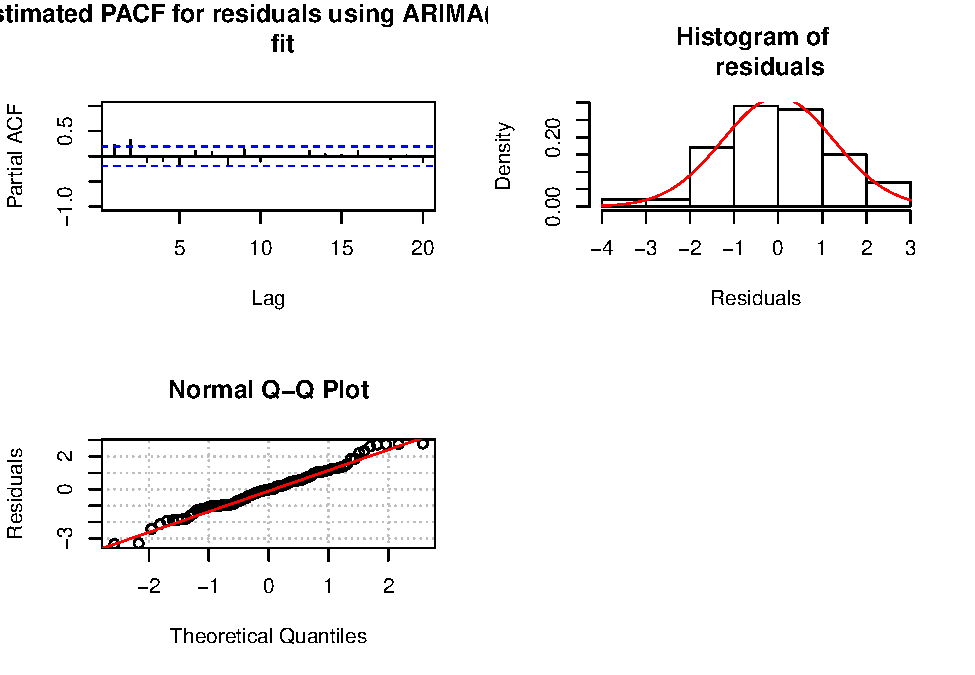
\includegraphics{06-Estimation-and-Inference_files/figure-latex/unnamed-chunk-15-1.pdf}

\begin{itemize}
\tightlist
\item
  The \texttt{ts()} function converts the time series data to an object that R recognizes as a time series.\\
\item
  The \texttt{lag()} function is used to find xt-1, xt-2, and xt-3. The k argument specifies how many time periods to go back. Run \texttt{lag(x.ts,\ k\ =\ -1)} and \texttt{lag(x.ts,\ k\ =\ 1)}to see what happens. To get everything lined up as I wanted with \texttt{ts.intersect()}, I chose to use k = -1.
\end{itemize}

\begin{Shaded}
\begin{Highlighting}[]
\FunctionTok{lag}\NormalTok{(x.ts, }\AttributeTok{k =} \SpecialCharTok{{-}}\DecValTok{1}\NormalTok{) }\CommentTok{\#shift down one time period(forward)}
\end{Highlighting}
\end{Shaded}

\begin{verbatim}
## Time Series:
## Start = 2 
## End = 101 
## Frequency = 1 
##   [1]  0.04172680  0.37190682 -0.18545185 -1.38297422 -2.87593652 -2.60017605
##   [7] -1.10401719 -0.46385116  0.80339069  2.11483585  3.39124978  3.86739194
##  [13]  2.12733595  0.67590604  0.71429367  0.38928044 -1.22681923  0.02287443
##  [19] -0.57321924 -2.68376851 -4.80850095 -2.44797633 -1.73921817 -1.48773023
##  [25]  0.68920966  0.40220308 -1.58781041 -2.07300848 -2.63408197 -3.54333559
##  [31] -2.74116328 -2.54401750 -3.19570817 -0.02623669  0.41663974 -1.74485791
##  [37] -3.04847994 -1.64692948 -1.71478199  0.11340965  1.55017869  0.47317192
##  [43] -0.18521791 -0.05759091 -1.32105323 -1.22071881 -1.53827085  0.01277076
##  [49] -3.19955388 -3.11022833 -3.30621969 -2.00546537  0.18084415  0.58776479
##  [55] -0.70238414 -0.34570939  0.94209248 -0.78176791  1.30547320 -1.04054783
##  [61] -1.06897160 -1.08850000  0.06031172 -0.05724856 -1.14731083 -0.79262221
##  [67] -0.55565451 -1.55985750 -2.17062644 -1.07776017  0.51569067  2.30660050
##  [73]  1.53530426  2.55899301  1.83836277  1.08072014  1.34125182 -0.80729300
##  [79] -1.42735924 -0.42456207 -0.11625003 -0.74807460  0.70052717  0.08557377
##  [85] -0.06039041  0.04479407 -0.12657328 -1.30097021  0.81586192 -0.13139757
##  [91]  1.84725644  1.62364752  0.33080663 -0.40824385 -1.56008530 -1.63175408
##  [97] -1.36418639 -0.37209392 -0.65833401  2.03705932
\end{verbatim}

\begin{Shaded}
\begin{Highlighting}[]
\FunctionTok{lag}\NormalTok{(x.ts, }\AttributeTok{k =} \DecValTok{0}\NormalTok{)}
\end{Highlighting}
\end{Shaded}

\begin{verbatim}
## Time Series:
## Start = 1 
## End = 100 
## Frequency = 1 
##   [1]  0.04172680  0.37190682 -0.18545185 -1.38297422 -2.87593652 -2.60017605
##   [7] -1.10401719 -0.46385116  0.80339069  2.11483585  3.39124978  3.86739194
##  [13]  2.12733595  0.67590604  0.71429367  0.38928044 -1.22681923  0.02287443
##  [19] -0.57321924 -2.68376851 -4.80850095 -2.44797633 -1.73921817 -1.48773023
##  [25]  0.68920966  0.40220308 -1.58781041 -2.07300848 -2.63408197 -3.54333559
##  [31] -2.74116328 -2.54401750 -3.19570817 -0.02623669  0.41663974 -1.74485791
##  [37] -3.04847994 -1.64692948 -1.71478199  0.11340965  1.55017869  0.47317192
##  [43] -0.18521791 -0.05759091 -1.32105323 -1.22071881 -1.53827085  0.01277076
##  [49] -3.19955388 -3.11022833 -3.30621969 -2.00546537  0.18084415  0.58776479
##  [55] -0.70238414 -0.34570939  0.94209248 -0.78176791  1.30547320 -1.04054783
##  [61] -1.06897160 -1.08850000  0.06031172 -0.05724856 -1.14731083 -0.79262221
##  [67] -0.55565451 -1.55985750 -2.17062644 -1.07776017  0.51569067  2.30660050
##  [73]  1.53530426  2.55899301  1.83836277  1.08072014  1.34125182 -0.80729300
##  [79] -1.42735924 -0.42456207 -0.11625003 -0.74807460  0.70052717  0.08557377
##  [85] -0.06039041  0.04479407 -0.12657328 -1.30097021  0.81586192 -0.13139757
##  [91]  1.84725644  1.62364752  0.33080663 -0.40824385 -1.56008530 -1.63175408
##  [97] -1.36418639 -0.37209392 -0.65833401  2.03705932
\end{verbatim}

\begin{Shaded}
\begin{Highlighting}[]
\FunctionTok{lag}\NormalTok{(x.ts, }\AttributeTok{k =} \DecValTok{1}\NormalTok{)}
\end{Highlighting}
\end{Shaded}

\begin{verbatim}
## Time Series:
## Start = 0 
## End = 99 
## Frequency = 1 
##   [1]  0.04172680  0.37190682 -0.18545185 -1.38297422 -2.87593652 -2.60017605
##   [7] -1.10401719 -0.46385116  0.80339069  2.11483585  3.39124978  3.86739194
##  [13]  2.12733595  0.67590604  0.71429367  0.38928044 -1.22681923  0.02287443
##  [19] -0.57321924 -2.68376851 -4.80850095 -2.44797633 -1.73921817 -1.48773023
##  [25]  0.68920966  0.40220308 -1.58781041 -2.07300848 -2.63408197 -3.54333559
##  [31] -2.74116328 -2.54401750 -3.19570817 -0.02623669  0.41663974 -1.74485791
##  [37] -3.04847994 -1.64692948 -1.71478199  0.11340965  1.55017869  0.47317192
##  [43] -0.18521791 -0.05759091 -1.32105323 -1.22071881 -1.53827085  0.01277076
##  [49] -3.19955388 -3.11022833 -3.30621969 -2.00546537  0.18084415  0.58776479
##  [55] -0.70238414 -0.34570939  0.94209248 -0.78176791  1.30547320 -1.04054783
##  [61] -1.06897160 -1.08850000  0.06031172 -0.05724856 -1.14731083 -0.79262221
##  [67] -0.55565451 -1.55985750 -2.17062644 -1.07776017  0.51569067  2.30660050
##  [73]  1.53530426  2.55899301  1.83836277  1.08072014  1.34125182 -0.80729300
##  [79] -1.42735924 -0.42456207 -0.11625003 -0.74807460  0.70052717  0.08557377
##  [85] -0.06039041  0.04479407 -0.12657328 -1.30097021  0.81586192 -0.13139757
##  [91]  1.84725644  1.62364752  0.33080663 -0.40824385 -1.56008530 -1.63175408
##  [97] -1.36418639 -0.37209392 -0.65833401  2.03705932
\end{verbatim}

\begin{Shaded}
\begin{Highlighting}[]
\CommentTok{\# 創建一個時間序列 x.ts}
\NormalTok{b.ts }\OtherTok{\textless{}{-}} \FunctionTok{ts}\NormalTok{(}\FunctionTok{c}\NormalTok{(}\DecValTok{10}\NormalTok{, }\DecValTok{20}\NormalTok{, }\DecValTok{30}\NormalTok{, }\DecValTok{40}\NormalTok{, }\DecValTok{50}\NormalTok{, }\DecValTok{60}\NormalTok{), }\AttributeTok{start =} \FunctionTok{c}\NormalTok{(}\DecValTok{2022}\NormalTok{, }\DecValTok{1}\NormalTok{), }\AttributeTok{frequency =} \DecValTok{12}\NormalTok{)}

\CommentTok{\# 使用 ts.intersect() 函數合併 x.ts 和它的三個 lag 時間序列}
\FunctionTok{ts.intersect}\NormalTok{(b.ts, }\AttributeTok{b.ts1 =} \FunctionTok{lag}\NormalTok{(}\AttributeTok{x =}\NormalTok{ b.ts, }\AttributeTok{k =} \SpecialCharTok{{-}}\DecValTok{1}\NormalTok{), }\AttributeTok{b.ts2 =} \FunctionTok{lag}\NormalTok{(}\AttributeTok{x =}\NormalTok{ b.ts, }\AttributeTok{k =} \SpecialCharTok{{-}}\DecValTok{2}\NormalTok{), }\AttributeTok{b.ts3 =} \FunctionTok{lag}\NormalTok{(}\AttributeTok{x =}\NormalTok{ b.ts, }\AttributeTok{k =} \SpecialCharTok{{-}}\DecValTok{3}\NormalTok{))}
\end{Highlighting}
\end{Shaded}

\begin{verbatim}
##          b.ts b.ts1 b.ts2 b.ts3
## Apr 2022   40    30    20    10
## May 2022   50    40    30    20
## Jun 2022   60    50    40    30
\end{verbatim}

\begin{Shaded}
\begin{Highlighting}[]
\CommentTok{\#b.ts1、b.ts2 和 b.ts3 的時間點是 b.ts 的時間點往後推 1、2、3 個時間單位。}
\NormalTok{b.ts1 }\OtherTok{=} \FunctionTok{lag}\NormalTok{(}\AttributeTok{x =}\NormalTok{ b.ts, }\AttributeTok{k =} \SpecialCharTok{{-}}\DecValTok{1}\NormalTok{)}
\NormalTok{b.ts2 }\OtherTok{=} \FunctionTok{lag}\NormalTok{(}\AttributeTok{x =}\NormalTok{ b.ts, }\AttributeTok{k =} \SpecialCharTok{{-}}\DecValTok{2}\NormalTok{)}
\NormalTok{b.ts3 }\OtherTok{=} \FunctionTok{lag}\NormalTok{(}\AttributeTok{x =}\NormalTok{ b.ts, }\AttributeTok{k =} \SpecialCharTok{{-}}\DecValTok{3}\NormalTok{)}
\NormalTok{b.ts}
\end{Highlighting}
\end{Shaded}

\begin{verbatim}
##      Jan Feb Mar Apr May Jun
## 2022  10  20  30  40  50  60
\end{verbatim}

\begin{Shaded}
\begin{Highlighting}[]
\NormalTok{b.ts1}
\end{Highlighting}
\end{Shaded}

\begin{verbatim}
##      Feb Mar Apr May Jun Jul
## 2022  10  20  30  40  50  60
\end{verbatim}

\begin{Shaded}
\begin{Highlighting}[]
\NormalTok{b.ts2}
\end{Highlighting}
\end{Shaded}

\begin{verbatim}
##      Mar Apr May Jun Jul Aug
## 2022  10  20  30  40  50  60
\end{verbatim}

\begin{Shaded}
\begin{Highlighting}[]
\NormalTok{b.ts3}
\end{Highlighting}
\end{Shaded}

\begin{verbatim}
##      Apr May Jun Jul Aug Sep
## 2022  10  20  30  40  50  60
\end{verbatim}

\begin{itemize}
\tightlist
\item
  The \texttt{ts.intersect()} function finds the intersection of the four different ``variables''.\\
\item
  The\texttt{cor()}function finds the estimated Pearson correlation coefficients between all variable pairs. Notice how close these correlations are to the autocorrelations!\\
\item
  The \texttt{scatterplotMatrix()} function finds a scatter plot matrix. The function is in the car package.
\end{itemize}

\begin{Shaded}
\begin{Highlighting}[]
\CommentTok{\#Used for estimation later in course}

\NormalTok{  gamma.x }\OtherTok{\textless{}{-}} \FunctionTok{acf}\NormalTok{(}\AttributeTok{x =}\NormalTok{ x, }\AttributeTok{type =} \StringTok{"covariance"}\NormalTok{, }\AttributeTok{main =}
    \FunctionTok{expression}\NormalTok{(}\FunctionTok{paste}\NormalTok{(}\StringTok{"Data simulated from AR(1): "}\NormalTok{, x[t] }\SpecialCharTok{==} \FloatTok{0.7}\SpecialCharTok{*}\NormalTok{x[t}\DecValTok{{-}1}\NormalTok{] }\SpecialCharTok{+}\NormalTok{ w[t], }\StringTok{" where "}\NormalTok{, w[t], }\StringTok{"\textasciitilde{}N(0,1)"}\NormalTok{)))}
\end{Highlighting}
\end{Shaded}

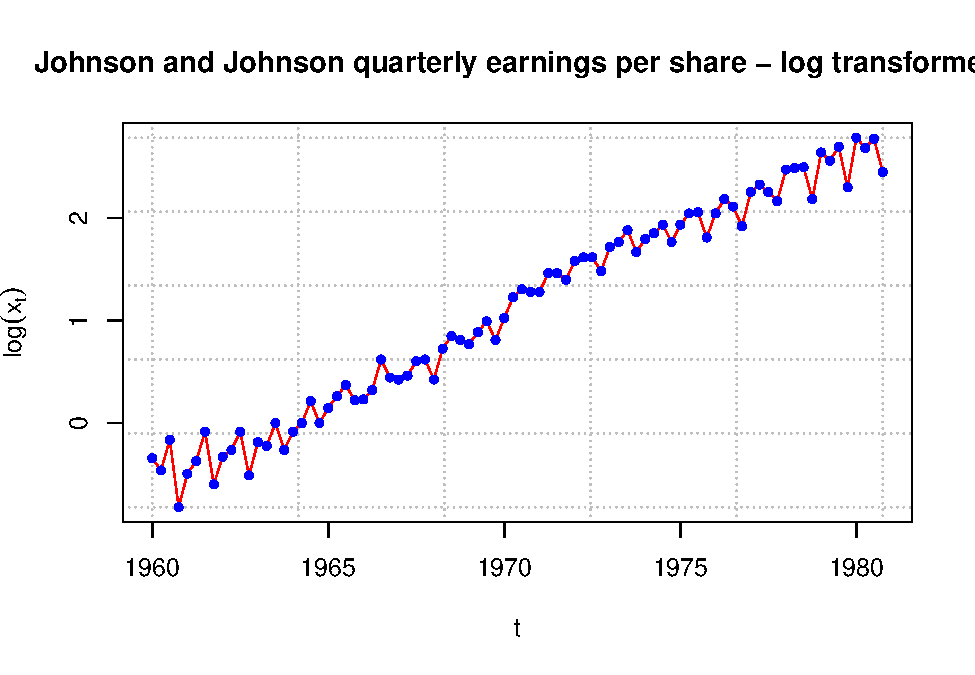
\includegraphics{06-Estimation-and-Inference_files/figure-latex/unnamed-chunk-21-1.pdf}

\begin{Shaded}
\begin{Highlighting}[]
\NormalTok{  gamma.x}
\end{Highlighting}
\end{Shaded}

\begin{verbatim}
## 
## Autocovariances of series 'x', by lag
## 
##       0       1       2       3       4       5       6       7       8       9 
##  2.5033  1.6864  1.0036  0.4219 -0.0586 -0.3120 -0.1687 -0.1608 -0.1445  0.0133 
##      10      11      12      13      14      15      16      17      18      19 
## -0.1102 -0.1029 -0.0430  0.1599  0.1892  0.3997  0.4790  0.3529  0.2015  0.0140 
##      20 
## -0.3293
\end{verbatim}

\begin{Shaded}
\begin{Highlighting}[]
  \FunctionTok{mean}\NormalTok{(x)}
\end{Highlighting}
\end{Shaded}

\begin{verbatim}
## [1] -0.4963419
\end{verbatim}

\begin{example}

\textbf{OSU enrollment data}

Click \href{http://www.chrisbilder.com/stat878/sections/2/OSU_enroll.csv}{here} to download data.

\begin{Shaded}
\begin{Highlighting}[]
\NormalTok{  osu.enroll }\OtherTok{\textless{}{-}} \FunctionTok{read.csv}\NormalTok{(}\AttributeTok{file =} \StringTok{"OSU\_enroll.csv"}\NormalTok{, }\AttributeTok{stringsAsFactors =} \ConstantTok{TRUE}\NormalTok{)}
  \FunctionTok{head}\NormalTok{(osu.enroll)}
\end{Highlighting}
\end{Shaded}

\begin{verbatim}
##   t Semester Year Enrollment      date
## 1 1     Fall 1989      20110 8/31/1989
## 2 2   Spring 1990      19128  2/1/1990
## 3 3   Summer 1990       7553  6/1/1990
## 4 4     Fall 1990      19591 8/31/1990
## 5 5   Spring 1991      18361  2/1/1991
## 6 6   Summer 1991       6702  6/1/1991
\end{verbatim}

\begin{Shaded}
\begin{Highlighting}[]
  \FunctionTok{tail}\NormalTok{(osu.enroll)}
\end{Highlighting}
\end{Shaded}

\begin{verbatim}
##     t Semester Year Enrollment      date
## 35 35   Spring 2001      20004  2/1/2001
## 36 36   Summer 2001       7558  6/1/2001
## 37 37     Fall 2001      21872 8/31/2001
## 38 38   Spring 2002      20922  2/1/2002
## 39 39   Summer 2002       7868  6/1/2002
## 40 40     Fall 2002      22992 8/31/2002
\end{verbatim}

\begin{Shaded}
\begin{Highlighting}[]
\NormalTok{  x }\OtherTok{\textless{}{-}}\NormalTok{ osu.enroll}\SpecialCharTok{$}\NormalTok{Enrollment}
\end{Highlighting}
\end{Shaded}

\begin{Shaded}
\begin{Highlighting}[]
\NormalTok{  rho.x }\OtherTok{\textless{}{-}} \FunctionTok{acf}\NormalTok{(}\AttributeTok{x =}\NormalTok{ x, }\AttributeTok{type =} \StringTok{"correlation"}\NormalTok{, }\AttributeTok{main =} \StringTok{"OSU Enrollment series"}\NormalTok{)}
\end{Highlighting}
\end{Shaded}

\includegraphics{06-Estimation-and-Inference_files/figure-latex/unnamed-chunk-23-1.pdf}

\begin{Shaded}
\begin{Highlighting}[]
\NormalTok{  rho.x}
\end{Highlighting}
\end{Shaded}

\begin{verbatim}
## 
## Autocorrelations of series 'x', by lag
## 
##      0      1      2      3      4      5      6      7      8      9     10 
##  1.000 -0.470 -0.425  0.909 -0.438 -0.395  0.822 -0.403 -0.358  0.739 -0.367 
##     11     12     13     14     15     16 
## -0.327  0.655 -0.337 -0.297  0.581 -0.309
\end{verbatim}

\begin{Shaded}
\begin{Highlighting}[]
\NormalTok{  rho.x}\SpecialCharTok{$}\NormalTok{acf[}\DecValTok{1}\SpecialCharTok{:}\DecValTok{9}\NormalTok{]}
\end{Highlighting}
\end{Shaded}

\begin{verbatim}
## [1]  1.0000000 -0.4702315 -0.4253427  0.9087421 -0.4377336 -0.3946048  0.8224660
## [8] -0.4025871 -0.3584216
\end{verbatim}

\end{example}

Notes:

\begin{itemize}
\tightlist
\item
  There are some large autocorrelations. This is a characteristic of a nonstationary series (seasonal factor). We will examine this more later.
\item
  Because the series is not stationary, the hypothesis test for \(\rho(h)\) = 0 should not be done here using the methods discussed earlier.\\
\item
  There is a pattern among the autocorrelations. What does this correspond to? (seasonal factor) (similar value/behavior happens during specific period of time/months across different years)
\end{itemize}

\hypertarget{resolving-non-stationarity-problems}{%
\chapter{Resolving Non-Stationarity Problems}\label{resolving-non-stationarity-problems}}

\hypertarget{differencing}{%
\section{Differencing}\label{differencing}}

Differencing helps to create the constant mean needed for stationarity. We will use differencing a lot!

1st differences: \(x_t – x_{t-1} = \nabla x_t\)

2nd differences: \((x_t – x_{t-1}) – (x_{t-1} – x_{t-2}) = \nabla x_t – \nabla x_{t-1} = \nabla^2x_t\)

Taking ``differences'' between successive data values in the time series helps to remove trend. Specifically, 1st differences help remove linear trend and 2nd differences help remove quadratic trend.

Why does this work? Consider the linear trend model \(x_t = \beta_0 + \beta_1t\) where t = time and \$\beta\_1\ne\$0. Then

\[x_t – x_{t-1} =  \beta_0 + \beta_1t – [\beta_0 + \beta_1(t – 1)] = \beta_1\]
which is not dependent on t.

\begin{example}

\textbf{Non-stationarity in the mean}

Click \href{http://www.chrisbilder.com/stat878/sections/2/nonstat.mean.csv}{Here} to download data.

Below is the code for a plot of xt vs.~t and the ACF for xt.

\begin{Shaded}
\begin{Highlighting}[]
\NormalTok{nonstat.mean }\OtherTok{\textless{}{-}} \FunctionTok{read.csv}\NormalTok{(}\AttributeTok{file=}\StringTok{"nonstat.mean.csv"}\NormalTok{)}
\FunctionTok{head}\NormalTok{(nonstat.mean)}
\end{Highlighting}
\end{Shaded}

\begin{verbatim}
##   time     x
## 1    1  1.31
## 2    2 13.67
## 3    3  6.29
## 4    4 -0.95
## 5    5  9.59
## 6    6 -0.45
\end{verbatim}

\begin{Shaded}
\begin{Highlighting}[]
\FunctionTok{tail}\NormalTok{(nonstat.mean)}
\end{Highlighting}
\end{Shaded}

\begin{verbatim}
##     time      x
## 95    95  92.69
## 96    96  91.22
## 97    97 100.00
## 98    98 102.80
## 99    99  93.82
## 100  100 108.72
\end{verbatim}

\begin{Shaded}
\begin{Highlighting}[]
\FunctionTok{dev.new}\NormalTok{(}\AttributeTok{width=}\DecValTok{8}\NormalTok{, }\AttributeTok{height=}\DecValTok{6}\NormalTok{, }\AttributeTok{pointsize=}\DecValTok{10}\NormalTok{)}

\FunctionTok{plot}\NormalTok{(}\AttributeTok{x=}\NormalTok{nonstat.mean}\SpecialCharTok{$}\NormalTok{x, }\AttributeTok{ylab=}\FunctionTok{expression}\NormalTok{(x[t]), }\AttributeTok{xlab=}\StringTok{"t (time)"}\NormalTok{, }\AttributeTok{type=}\StringTok{"l"}\NormalTok{, }\AttributeTok{col=}\StringTok{"red"}\NormalTok{, }\AttributeTok{main=}\StringTok{"Nonstationary time series"}\NormalTok{, }\AttributeTok{panel.first=}\FunctionTok{grid}\NormalTok{(}\AttributeTok{col=}\StringTok{"gray"}\NormalTok{, }\AttributeTok{lty=}\StringTok{"dotted"}\NormalTok{))}

\FunctionTok{points}\NormalTok{(}\AttributeTok{x=}\NormalTok{nonstat.mean}\SpecialCharTok{$}\NormalTok{x, }\AttributeTok{col=}\StringTok{"blue"}\NormalTok{, }\AttributeTok{pch=}\DecValTok{20}\NormalTok{)}
\end{Highlighting}
\end{Shaded}

\begin{Shaded}
\begin{Highlighting}[]
\FunctionTok{acf}\NormalTok{(}\AttributeTok{x=}\NormalTok{nonstat.mean}\SpecialCharTok{$}\NormalTok{x, }\AttributeTok{type=}\StringTok{"correlation"}\NormalTok{, }\AttributeTok{main=}\StringTok{"Plot of the ACF"}\NormalTok{)}
\end{Highlighting}
\end{Shaded}

\includegraphics{07-Resolvin-non-stationarity_files/figure-latex/unnamed-chunk-3-1.pdf}
Whenever you see a ACF plot like this(high correlation), it's highly likely that there's a non-stationarity in mean.

\begin{Shaded}
\begin{Highlighting}[]
\CommentTok{\# scatter plot of x\_t vs. x\_t{-}1}
\NormalTok{x.ts }\OtherTok{\textless{}{-}} \FunctionTok{ts}\NormalTok{(nonstat.mean[,}\DecValTok{2}\NormalTok{])}
\NormalTok{set1 }\OtherTok{\textless{}{-}} \FunctionTok{ts.intersect}\NormalTok{(x.ts, }\AttributeTok{x.ts1=}\FunctionTok{lag}\NormalTok{(}\AttributeTok{x=}\NormalTok{x.ts, }\AttributeTok{k=}\SpecialCharTok{{-}}\DecValTok{1}\NormalTok{))}
\FunctionTok{head}\NormalTok{(set1)}
\end{Highlighting}
\end{Shaded}

\begin{verbatim}
##       x.ts x.ts1
## [1,] 13.67  1.31
## [2,]  6.29 13.67
## [3,] -0.95  6.29
## [4,]  9.59 -0.95
## [5,] -0.45  9.59
## [6,] 17.22 -0.45
\end{verbatim}

\begin{Shaded}
\begin{Highlighting}[]
\FunctionTok{cor}\NormalTok{(set1)}
\end{Highlighting}
\end{Shaded}

\begin{verbatim}
##           x.ts    x.ts1
## x.ts  1.000000 0.857779
## x.ts1 0.857779 1.000000
\end{verbatim}

\begin{Shaded}
\begin{Highlighting}[]
\CommentTok{\# Need as.numeric() so that plot.ts() is not run, want plot.default()}

\FunctionTok{plot}\NormalTok{(}\AttributeTok{y=}\FunctionTok{as.numeric}\NormalTok{(set1[,}\DecValTok{1}\NormalTok{]), }\AttributeTok{x=}\FunctionTok{as.numeric}\NormalTok{(set1[,}\DecValTok{2}\NormalTok{]), }\AttributeTok{ylab=}\FunctionTok{expression}\NormalTok{(x[t]), }\AttributeTok{type=}\StringTok{"p"}\NormalTok{, }\AttributeTok{xlab=}\FunctionTok{expression}\NormalTok{(x[t}\DecValTok{{-}1}\NormalTok{]))}
\end{Highlighting}
\end{Shaded}

\includegraphics{07-Resolvin-non-stationarity_files/figure-latex/unnamed-chunk-6-1.pdf}

\begin{Shaded}
\begin{Highlighting}[]
\CommentTok{\# you can see from the graph there\textquotesingle{}s a positive linear relationship, this is why the correlation is so high.}
\end{Highlighting}
\end{Shaded}

\end{example}

\begin{itemize}
\tightlist
\item
  This data is said to have ``nonstationarity in the mean'' because the mean of \(x_t, \mu_t,\) appears to be changing as a function of time.
\item
  Why is there large positive autocorrelation at lag = 1, 2, \ldots{} ?

  \begin{itemize}
  \tightlist
  \item
    This is b/c we have a positive linear relationship btw \(x_t\) and \(x_{t-1}\).
  \end{itemize}
\end{itemize}

Below is the code to find the first differences:

\begin{Shaded}
\begin{Highlighting}[]
\CommentTok{\# Find first differences}

\NormalTok{first.diff }\OtherTok{\textless{}{-}} \FunctionTok{diff}\NormalTok{(}\AttributeTok{x=}\NormalTok{nonstat.mean}\SpecialCharTok{$}\NormalTok{x, }\AttributeTok{lag=}\DecValTok{1}\NormalTok{, }\AttributeTok{differences=}\DecValTok{1}\NormalTok{)}
\NormalTok{first.diff[}\DecValTok{1}\SpecialCharTok{:}\DecValTok{5}\NormalTok{]}
\end{Highlighting}
\end{Shaded}

\begin{verbatim}
## [1]  12.36  -7.38  -7.24  10.54 -10.04
\end{verbatim}

\begin{Shaded}
\begin{Highlighting}[]
\NormalTok{nonstat.mean}\SpecialCharTok{$}\NormalTok{x[}\DecValTok{2}\NormalTok{]}\SpecialCharTok{{-}}\NormalTok{nonstat.mean}\SpecialCharTok{$}\NormalTok{x[}\DecValTok{1}\NormalTok{]}
\end{Highlighting}
\end{Shaded}

\begin{verbatim}
## [1] 12.36
\end{verbatim}

\begin{Shaded}
\begin{Highlighting}[]
\NormalTok{nonstat.mean}\SpecialCharTok{$}\NormalTok{x[}\DecValTok{3}\NormalTok{]}\SpecialCharTok{{-}}\NormalTok{nonstat.mean}\SpecialCharTok{$}\NormalTok{x[}\DecValTok{2}\NormalTok{]}
\end{Highlighting}
\end{Shaded}

\begin{verbatim}
## [1] -7.38
\end{verbatim}

\begin{Shaded}
\begin{Highlighting}[]
\FunctionTok{plot}\NormalTok{(}\AttributeTok{x=}\NormalTok{ first.diff, }\AttributeTok{ylab=}\FunctionTok{expression}\NormalTok{(x[t]}\SpecialCharTok{{-}}\NormalTok{x[t}\DecValTok{{-}1}\NormalTok{]), }\AttributeTok{xlab=}\StringTok{"t (time)"}\NormalTok{, }\AttributeTok{type=}\StringTok{"l"}\NormalTok{, }\AttributeTok{col=}\StringTok{"red"}\NormalTok{, }\AttributeTok{main=}\StringTok{"First differences"}\NormalTok{, }\AttributeTok{panel.first =} \FunctionTok{grid}\NormalTok{(}\AttributeTok{col=}\StringTok{"gray"}\NormalTok{,}\AttributeTok{lty=}\StringTok{"dotted"}\NormalTok{))}

\FunctionTok{points}\NormalTok{(}\AttributeTok{x=}\NormalTok{first.diff, }\AttributeTok{col=}\StringTok{"blue"}\NormalTok{, }\AttributeTok{pch=}\DecValTok{20}\NormalTok{)}
\end{Highlighting}
\end{Shaded}

\includegraphics{07-Resolvin-non-stationarity_files/figure-latex/unnamed-chunk-8-1.pdf}
The linear relationship just disappears after first differencing!

\begin{Shaded}
\begin{Highlighting}[]
\FunctionTok{acf}\NormalTok{(}\AttributeTok{x=}\NormalTok{first.diff, }\AttributeTok{type=}\StringTok{"correlation"}\NormalTok{, }\AttributeTok{main=}\StringTok{"Plot of the ACF for first differences"}\NormalTok{)}
\end{Highlighting}
\end{Shaded}

\includegraphics{07-Resolvin-non-stationarity_files/figure-latex/unnamed-chunk-9-1.pdf}

If you want xt and xt - xt-1 in the same data frame, use the \texttt{ts.intersect()} function:

\begin{Shaded}
\begin{Highlighting}[]
\NormalTok{x }\OtherTok{\textless{}{-}} \FunctionTok{ts}\NormalTok{(}\AttributeTok{data=}\NormalTok{nonstat.mean}\SpecialCharTok{$}\NormalTok{x)}
\NormalTok{x.diff1 }\OtherTok{\textless{}{-}} \FunctionTok{ts}\NormalTok{(}\AttributeTok{data=}\NormalTok{first.diff, }\AttributeTok{start=}\DecValTok{2}\NormalTok{)}
\FunctionTok{ts.intersect}\NormalTok{(x, x.diff1)}
\end{Highlighting}
\end{Shaded}

\begin{verbatim}
## Time Series:
## Start = 2 
## End = 100 
## Frequency = 1 
##          x x.diff1
##   2  13.67   12.36
##   3   6.29   -7.38
##   4  -0.95   -7.24
##   5   9.59   10.54
##   6  -0.45  -10.04
##   7  17.22   17.67
##   8  -6.88  -24.10
##   9  10.36   17.24
##  10  12.53    2.17
##  11   4.22   -8.31
##  12  17.19   12.97
##  13  26.02    8.83
##  14  19.14   -6.88
##  15  23.55    4.41
##  16  30.05    6.50
##  17  21.61   -8.44
##  18  26.86    5.25
##  19  36.59    9.73
##  20  10.67  -25.92
##  21  26.58   15.91
##  22  19.81   -6.77
##  23  31.54   11.73
##  24  22.74   -8.80
##  25  37.87   15.13
##  26  35.86   -2.01
##  27  48.18   12.32
##  28  36.16  -12.02
##  29  37.10    0.94
##  30  43.03    5.93
##  31  27.79  -15.24
##  32  33.05    5.26
##  33  22.76  -10.29
##  34  36.72   13.96
##  35  43.67    6.95
##  36  31.76  -11.91
##  37  37.28    5.52
##  38  46.81    9.53
##  39  37.46   -9.35
##  40  46.50    9.04
##  41  35.61  -10.89
##  42  48.56   12.95
##  43  43.68   -4.88
##  44  46.54    2.86
##  45  62.40   15.86
##  46  28.79  -33.61
##  47  47.88   19.09
##  48  49.36    1.48
##  49  77.58   28.22
##  50  41.47  -36.11
##  51  54.95   13.48
##  52  24.10  -30.85
##  53  27.68    3.58
##  54  55.36   27.68
##  55  41.44  -13.92
##  56  76.86   35.42
##  57  51.43  -25.43
##  58  41.03  -10.40
##  59  51.94   10.91
##  60  47.14   -4.80
##  61  54.05    6.91
##  62  48.72   -5.33
##  63  53.41    4.69
##  64  69.12   15.71
##  65  83.26   14.14
##  66  62.53  -20.73
##  67  76.77   14.24
##  68  52.98  -23.79
##  69  61.83    8.85
##  70  67.64    5.81
##  71  66.08   -1.56
##  72  80.28   14.20
##  73  87.40    7.12
##  74  88.11    0.71
##  75  65.85  -22.26
##  76  82.29   16.44
##  77  97.92   15.63
##  78  79.62  -18.30
##  79  81.30    1.68
##  80  58.63  -22.67
##  81  89.71   31.08
##  82  85.11   -4.60
##  83  70.66  -14.45
##  84  74.24    3.58
##  85  74.27    0.03
##  86  66.52   -7.75
##  87  85.93   19.41
##  88  95.23    9.30
##  89  87.26   -7.97
##  90  74.88  -12.38
##  91  73.44   -1.44
##  92  89.44   16.00
##  93  62.11  -27.33
##  94  90.01   27.90
##  95  92.69    2.68
##  96  91.22   -1.47
##  97 100.00    8.78
##  98 102.80    2.80
##  99  93.82   -8.98
## 100 108.72   14.90
\end{verbatim}

Why does the data set start at 2?

Other types of differencing:

\begin{itemize}
\tightlist
\item
  2nd differences: \texttt{diff(x,\ lag\ =\ 1,\ differences\ =\ 2)}
\item
  xt -- xt-2: \texttt{diff(x,\ lag\ =\ 2,\ differences\ =\ 1)}; this can be useful when there is a ``seasonal'' trend
\end{itemize}

\begin{Shaded}
\begin{Highlighting}[]
\CommentTok{\# Second differences}
\FunctionTok{diff}\NormalTok{(x, }\AttributeTok{lag =} \DecValTok{1}\NormalTok{, }\AttributeTok{differences=}\DecValTok{2}\NormalTok{)}
\end{Highlighting}
\end{Shaded}

\begin{verbatim}
## Time Series:
## Start = 3 
## End = 100 
## Frequency = 1 
##  [1] -19.74   0.14  17.78 -20.58  27.71 -41.77  41.34 -15.07 -10.48  21.28
## [11]  -4.14 -15.71  11.29   2.09 -14.94  13.69   4.48 -35.65  41.83 -22.68
## [21]  18.50 -20.53  23.93 -17.14  14.33 -24.34  12.96   4.99 -21.17  20.50
## [31] -15.55  24.25  -7.01 -18.86  17.43   4.01 -18.88  18.39 -19.93  23.84
## [41] -17.83   7.74  13.00 -49.47  52.70 -17.61  26.74 -64.33  49.59 -44.33
## [51]  34.43  24.10 -41.60  49.34 -60.85  15.03  21.31 -15.71  11.71 -12.24
## [61]  10.02  11.02  -1.57 -34.87  34.97 -38.03  32.64  -3.04  -7.37  15.76
## [71]  -7.08  -6.41 -22.97  38.70  -0.81 -33.93  19.98 -24.35  53.75 -35.68
## [81]  -9.85  18.03  -3.55  -7.78  27.16 -10.11 -17.27  -4.41  10.94  17.44
## [91] -43.33  55.23 -25.22  -4.15  10.25  -5.98 -11.78  23.88
\end{verbatim}

\begin{Shaded}
\begin{Highlighting}[]
\NormalTok{(nonstat.mean}\SpecialCharTok{$}\NormalTok{x[}\DecValTok{3}\NormalTok{] }\SpecialCharTok{{-}}\NormalTok{ nonstat.mean}\SpecialCharTok{$}\NormalTok{x[}\DecValTok{2}\NormalTok{]) }\SpecialCharTok{{-}}\NormalTok{ (nonstat.mean}\SpecialCharTok{$}\NormalTok{x[}\DecValTok{2}\NormalTok{] }\SpecialCharTok{{-}}\NormalTok{ nonstat.mean}\SpecialCharTok{$}\NormalTok{x[}\DecValTok{1}\NormalTok{])}
\end{Highlighting}
\end{Shaded}

\begin{verbatim}
## [1] -19.74
\end{verbatim}

\begin{Shaded}
\begin{Highlighting}[]
\CommentTok{\# x\_t {-} x\_t{-}2}
\FunctionTok{diff}\NormalTok{(x, }\AttributeTok{lag =} \DecValTok{2}\NormalTok{, }\AttributeTok{differences =} \DecValTok{1}\NormalTok{)}
\end{Highlighting}
\end{Shaded}

\begin{verbatim}
## Time Series:
## Start = 3 
## End = 100 
## Frequency = 1 
##  [1]   4.98 -14.62   3.30   0.50   7.63  -6.43  -6.86  19.41  -6.14   4.66
## [11]  21.80   1.95  -2.47  10.91  -1.94  -3.19  14.98 -16.19 -10.01   9.14
## [21]   4.96   2.93   6.33  13.12  10.31   0.30 -11.08   6.87  -9.31  -9.98
## [31]  -5.03   3.67  20.91  -4.96  -6.39  15.05   0.18  -0.31  -1.85   2.06
## [41]   8.07  -2.02  18.72 -17.75 -14.52  20.57  29.70  -7.89 -22.63 -17.37
## [51] -27.27  31.26  13.76  21.50   9.99 -35.83   0.51   6.11   2.11   1.58
## [61]  -0.64  20.40  29.85  -6.59  -6.49  -9.55 -14.94  14.66   4.25  12.64
## [71]  21.32   7.83 -21.55  -5.82  32.07  -2.67 -16.62 -20.99   8.41  26.48
## [81] -19.05 -10.87   3.61  -7.72  11.66  28.71   1.33 -20.35 -13.82  14.56
## [91] -11.33   0.57  30.58   1.21   7.31  11.58  -6.18   5.92
\end{verbatim}

\begin{Shaded}
\begin{Highlighting}[]
\NormalTok{nonstat.mean}\SpecialCharTok{$}\NormalTok{x[}\DecValTok{3}\NormalTok{] }\SpecialCharTok{{-}}\NormalTok{ nonstat.mean}\SpecialCharTok{$}\NormalTok{x[}\DecValTok{1}\NormalTok{]}
\end{Highlighting}
\end{Shaded}

\begin{verbatim}
## [1] 4.98
\end{verbatim}

\begin{Shaded}
\begin{Highlighting}[]
\CommentTok{\# Plot}
\FunctionTok{lag.plot}\NormalTok{(x, }\AttributeTok{lags =} \DecValTok{4}\NormalTok{, }\AttributeTok{layout =} \FunctionTok{c}\NormalTok{(}\DecValTok{2}\NormalTok{,}\DecValTok{2}\NormalTok{), }\AttributeTok{do.lines =} \ConstantTok{FALSE}\NormalTok{)}
\end{Highlighting}
\end{Shaded}

\includegraphics{07-Resolvin-non-stationarity_files/figure-latex/unnamed-chunk-13-1.pdf}

Note: There are formal hypothesis tests to determine if differencing is needed. This corresponds to an area of time series known as ``unit root'' testing. The name will be clear once we examine autoregressive models in detail.

\hypertarget{backshift-operator}{%
\section{Backshift Operator}\label{backshift-operator}}

A convenient way to represent differencing in time series models is to use the ``backshift operator''. It is denoted by ``B'' and defined as follows:
\[Bx_t=x_{t-1}\]
Notice that \(x_t\) moved back one-time period when the backshift operator was applied to it.

In general, \(B^2x_t = x_{t-2}, B^3x_t = x_{t-3}, …, and \quad B^kx_t = x_{t-k}.\)

Notes:

\begin{itemize}
\tightlist
\item
  Let C be a constant not indexed by time. Then \(BC = C.\)\\
\item
  \((1-B)x_t = x_t – x_{t-1} = \nabla x_t\)
\item
  \(B\times B = B^2\)
\item
  \[(1-B)^2x_t = (1 - 2B + B^2)x_t = x_t – 2Bx_t + B^2x_t\\
  = x_t – 2x_{t-1} + x_{t-2}\\
  = x_t – x_{t-1} – x_{t-1} + x_{t-2}\\ 
  = (x_t – x_{t-1}) – (x_{t-1} – x_{t-2})\\
  = \nabla^2x_t\]
\item
  \((1-B)^0x_t = x_t\)
\item
  \((1-B)x_t\) can be thought of as a ``linear filter'' since the linear trend is being filtered out of the time series.
\end{itemize}

\begin{example}
\textbf{Moving Average}

\(m_t=\frac{w_t+w_{t-1}+w_{t-2}}{3}\), where \(w_t \sim \mathrm{ind}N(0,\sigma^2_w) \forall t=1,..n\) can be represented by \((1+B+B^2)\frac{w_t}{3}\)
\end{example}

\begin{example}
\textbf{Autoregression}

\(x_t=0.7x_{t-1}+w_t\), where \(w_t \sim \mathrm{ind}N(0,\sigma^2_w) \forall t=1,..n\) can be represented by \((1-0.7B)x_t=w_t\)
\end{example}

\begin{example}
\textbf{first differencing needed example}

Consider the following model:

\((1-0.7B)(1-B)x_t=w_t\), where \(w_t \sim \mathrm{ind}N(0,\sigma^2_w) \forall t=1,..n\). This simplifies to

\[(1-0.7B)(x_t-x_{t-1})=w_t\\
\iff x_t-x_{t-1}-0.7Bx_t+0.7Bx_{t-1}=w_t\\
\iff x_t=x_{t-1}+0.7x_{t-1}-0.7x_{t-2}+w_t\\
\iff x_t=1.7x_{t-1}-0.7x_{t-2}+w_t\]

Later in the course, we will identify this as a ARIMA(1,1,0) model.

Suppose a realization of a time series is simulated from this model. Below is a plot of the data.

\begin{Shaded}
\begin{Highlighting}[]
\FunctionTok{set.seed}\NormalTok{(}\DecValTok{7328}\NormalTok{)  }
\NormalTok{w }\OtherTok{\textless{}{-}} \FunctionTok{rnorm}\NormalTok{(}\AttributeTok{n =} \DecValTok{200}\NormalTok{, }\AttributeTok{mean =} \DecValTok{0}\NormalTok{, }\AttributeTok{sd =} \DecValTok{1}\NormalTok{)}

\NormalTok{x }\OtherTok{\textless{}{-}} \FunctionTok{numeric}\NormalTok{(}\AttributeTok{length =} \DecValTok{200}\NormalTok{)}
\NormalTok{x}\FloatTok{.1} \OtherTok{\textless{}{-}} \DecValTok{0}
\NormalTok{x}\FloatTok{.2} \OtherTok{\textless{}{-}} \DecValTok{0}
\ControlFlowTok{for}\NormalTok{ (i }\ControlFlowTok{in} \DecValTok{1}\SpecialCharTok{:}\FunctionTok{length}\NormalTok{(x)) \{}
\NormalTok{  x[i] }\OtherTok{\textless{}{-}} \FloatTok{1.7}\SpecialCharTok{*}\NormalTok{x}\FloatTok{.1} \SpecialCharTok{{-}} \FloatTok{0.7}\SpecialCharTok{*}\NormalTok{x}\FloatTok{.2} \SpecialCharTok{+}\NormalTok{ w[i] }
\NormalTok{  x}\FloatTok{.2} \OtherTok{\textless{}{-}}\NormalTok{ x}\FloatTok{.1}
\NormalTok{  x}\FloatTok{.1} \OtherTok{\textless{}{-}}\NormalTok{ x[i] }
\NormalTok{\}}

\CommentTok{\#Do not use first 100}
\NormalTok{X }\OtherTok{\textless{}{-}}\NormalTok{ x[}\DecValTok{101}\SpecialCharTok{:}\DecValTok{200}\NormalTok{]}
\end{Highlighting}
\end{Shaded}

\begin{Shaded}
\begin{Highlighting}[]
\FunctionTok{dev.new}\NormalTok{(}\AttributeTok{width =} \DecValTok{8}\NormalTok{, }\AttributeTok{height =} \DecValTok{6}\NormalTok{, }\AttributeTok{pointsize =} \DecValTok{10}\NormalTok{)      }
\FunctionTok{plot}\NormalTok{(}\AttributeTok{x =}\NormalTok{ X, }\AttributeTok{ylab =} \FunctionTok{expression}\NormalTok{(x[t]), }\AttributeTok{xlab =} \StringTok{"t"}\NormalTok{, }\AttributeTok{type =} 
    \StringTok{"l"}\NormalTok{, }\AttributeTok{col =} \StringTok{"red"}\NormalTok{, }\AttributeTok{lwd =} \DecValTok{1}\NormalTok{ , }\AttributeTok{main =} 
    \FunctionTok{expression}\NormalTok{(}\FunctionTok{paste}\NormalTok{(}\StringTok{"Data simulated from "}\NormalTok{, (}\DecValTok{1}\FloatTok{{-}0.7}\SpecialCharTok{*}\NormalTok{B)}\SpecialCharTok{*}\NormalTok{(}\DecValTok{1}\SpecialCharTok{{-}}
\NormalTok{    B)}\SpecialCharTok{*}\NormalTok{x[t] }\SpecialCharTok{==}\NormalTok{ w[t], }\StringTok{" where "}\NormalTok{, w[t], }\StringTok{"\textasciitilde{}N(0,1)"}\NormalTok{)), }
    \AttributeTok{panel.first=}\FunctionTok{grid}\NormalTok{(}\AttributeTok{col =} \StringTok{"gray"}\NormalTok{, }\AttributeTok{lty =} \StringTok{"dotted"}\NormalTok{))}
\FunctionTok{points}\NormalTok{(}\AttributeTok{x =}\NormalTok{ X, }\AttributeTok{pch =} \DecValTok{20}\NormalTok{, }\AttributeTok{col =} \StringTok{"blue"}\NormalTok{)}

\CommentTok{\# from the graph there\textquotesingle{}s nonstationarity in mean}
\end{Highlighting}
\end{Shaded}

\begin{Shaded}
\begin{Highlighting}[]
\FunctionTok{acf}\NormalTok{(}\AttributeTok{x=}\NormalTok{X, }\AttributeTok{type=}\StringTok{"correlation"}\NormalTok{, }\AttributeTok{main=}\StringTok{"Plot of the ACF"}\NormalTok{)}
\end{Highlighting}
\end{Shaded}

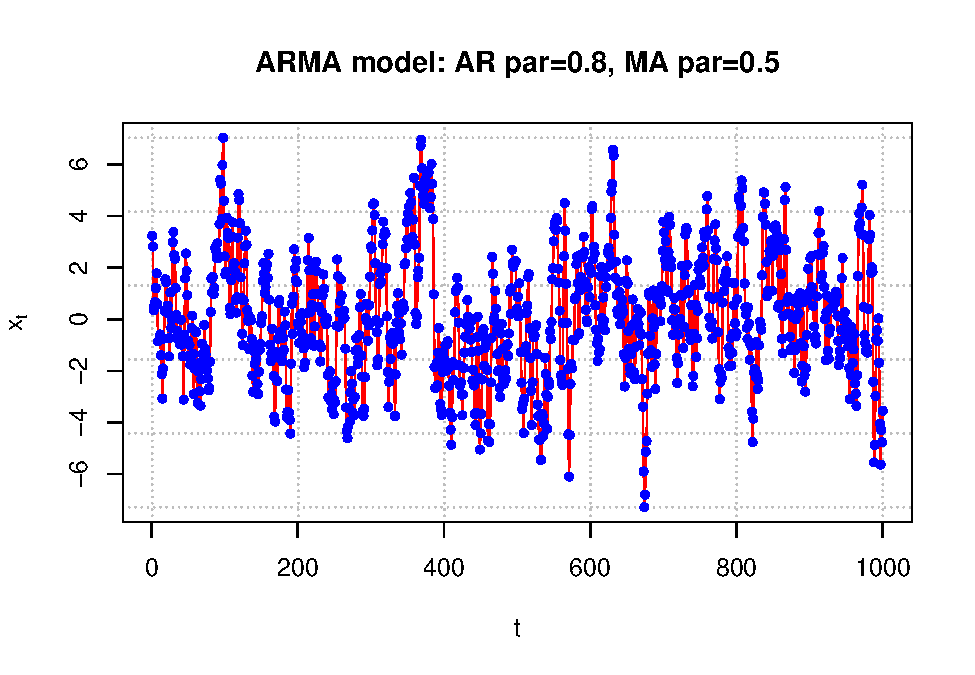
\includegraphics{07-Resolvin-non-stationarity_files/figure-latex/unnamed-chunk-16-1.pdf}

After the first differences:

\begin{Shaded}
\begin{Highlighting}[]
\CommentTok{\# Finf first differences}

\FunctionTok{plot}\NormalTok{(}\AttributeTok{x=}\FunctionTok{diff}\NormalTok{(}\AttributeTok{x=}\NormalTok{X, }\AttributeTok{lag=}\DecValTok{1}\NormalTok{, }\AttributeTok{differences =} \DecValTok{1}\NormalTok{), }\AttributeTok{ylab=}\FunctionTok{expression}\NormalTok{(x[t]}\SpecialCharTok{{-}}\NormalTok{x[t}\DecValTok{{-}1}\NormalTok{]), }\AttributeTok{xlab=}\StringTok{"t (time)"}\NormalTok{, }\AttributeTok{type=}\StringTok{"l"}\NormalTok{, }\AttributeTok{col=}\StringTok{"red"}\NormalTok{, }\AttributeTok{main=}\FunctionTok{expression}\NormalTok{(}\FunctionTok{paste}\NormalTok{(}\StringTok{"1st diff. for data simulated from "}\NormalTok{, (}\DecValTok{1}\FloatTok{{-}0.7}\SpecialCharTok{*}\NormalTok{B)}\SpecialCharTok{*}\NormalTok{(}\DecValTok{1}\SpecialCharTok{{-}}\NormalTok{B)}\SpecialCharTok{*}\NormalTok{x[t] }\SpecialCharTok{==}\NormalTok{ w[t], }\StringTok{" where }
\StringTok{   "}\NormalTok{, w[t], }\StringTok{"\textasciitilde{}N(0,1)"}\NormalTok{)), }\AttributeTok{panel.first=}\FunctionTok{grid}\NormalTok{(}\AttributeTok{col=}\StringTok{"gray"}\NormalTok{,}\AttributeTok{lty=}\StringTok{"dotted"}\NormalTok{))}
\end{Highlighting}
\end{Shaded}

\begin{verbatim}
## Warning in title(...): font metrics unknown for character 0xa

## Warning in title(...): font metrics unknown for character 0xa
\end{verbatim}

\begin{Shaded}
\begin{Highlighting}[]
\FunctionTok{points}\NormalTok{(}\AttributeTok{x=}\FunctionTok{diff}\NormalTok{(}\AttributeTok{x=}\NormalTok{X, }\AttributeTok{lag=}\DecValTok{1}\NormalTok{, }\AttributeTok{differences =} \DecValTok{1}\NormalTok{), }\AttributeTok{pch=}\DecValTok{20}\NormalTok{, }\AttributeTok{col=}\StringTok{"blue"}\NormalTok{)}
\end{Highlighting}
\end{Shaded}

\includegraphics{07-Resolvin-non-stationarity_files/figure-latex/unnamed-chunk-17-1.pdf}

\begin{Shaded}
\begin{Highlighting}[]
\FunctionTok{acf}\NormalTok{(}\AttributeTok{x=}\FunctionTok{diff}\NormalTok{(}\AttributeTok{x=}\NormalTok{X, }\AttributeTok{lag=}\DecValTok{1}\NormalTok{, }\AttributeTok{differences =} \DecValTok{1}\NormalTok{), }\AttributeTok{type=}\StringTok{"correlation"}\NormalTok{, }\AttributeTok{main=}\StringTok{"Plot of the ACF"}\NormalTok{)}
\end{Highlighting}
\end{Shaded}

\includegraphics{07-Resolvin-non-stationarity_files/figure-latex/unnamed-chunk-18-1.pdf}

An easier way is to use \texttt{arima.sim()} to simulate the data.
\end{example}

\hypertarget{fractional-differencing}{%
\section{Fractional Differencing}\label{fractional-differencing}}

Use fractional powers of B between --0.5 to 0.5 to do the differencing. This is used with long-memory time series.

Notes:

\begin{itemize}
\tightlist
\item
  Differencing is often used to help make a nonstationary in the mean time series stationary. Unfortunately in real applications, we do not know what exact level of differencing is needed (we can approximate it). If a too high of level of differencing is done, this can hurt a time series model. As a compromise between differencing and not differencing at all, fractional differencing can be used.\\
\item
  The reason why these are called a ``long memory'' time series can be seen from a ``short memory'' time series. A short memory stationary process will have \(\rho(h)\to 0\) ``quickly'' as \(h\to \infty\). A long memory time series does not and has \(\rho(h)\to 0\) ``slowly''. More on this later in the course.
\item
  The fractional difference series can be represented as \[\nabla^dx_t=\sum_{j=0}^{\infty}\pi_jx_{t-j}\]
\end{itemize}

where the \(\pi_j\) are found through a Taylor series expansion of \((1-B)^d\).

\hypertarget{transformations}{%
\section{Transformations}\label{transformations}}

In regression analysis, transformations of the response variable are taken to induce approximate constant variance. In a similar manner, we can take transformations of xt to help make a nonstationary in the variance time series be approximately stationary in the variance.

\begin{example}
\textbf{Johnson \& Johnson earnings per share data}

This data comes from Shumway and Stoffer's book.

\begin{Shaded}
\begin{Highlighting}[]
\FunctionTok{library}\NormalTok{(astsa)}
\NormalTok{x }\OtherTok{\textless{}{-}}\NormalTok{ jj}
\NormalTok{x}
\end{Highlighting}
\end{Shaded}

\begin{verbatim}
##           Qtr1      Qtr2      Qtr3      Qtr4
## 1960  0.710000  0.630000  0.850000  0.440000
## 1961  0.610000  0.690000  0.920000  0.550000
## 1962  0.720000  0.770000  0.920000  0.600000
## 1963  0.830000  0.800000  1.000000  0.770000
## 1964  0.920000  1.000000  1.240000  1.000000
## 1965  1.160000  1.300000  1.450000  1.250000
## 1966  1.260000  1.380000  1.860000  1.560000
## 1967  1.530000  1.590000  1.830000  1.860000
## 1968  1.530000  2.070000  2.340000  2.250000
## 1969  2.160000  2.430000  2.700000  2.250000
## 1970  2.790000  3.420000  3.690000  3.600000
## 1971  3.600000  4.320000  4.320000  4.050000
## 1972  4.860000  5.040000  5.040000  4.410000
## 1973  5.580000  5.850000  6.570000  5.310000
## 1974  6.030000  6.390000  6.930000  5.850000
## 1975  6.930000  7.740000  7.830000  6.120000
## 1976  7.740000  8.910000  8.280000  6.840000
## 1977  9.540000 10.260000  9.540000  8.729999
## 1978 11.880000 12.060000 12.150000  8.910000
## 1979 14.040000 12.960000 14.850000  9.990000
## 1980 16.200000 14.670000 16.020000 11.610000
\end{verbatim}

\begin{Shaded}
\begin{Highlighting}[]
\FunctionTok{dev.new}\NormalTok{(}\AttributeTok{width =} \DecValTok{8}\NormalTok{, }\AttributeTok{height =} \DecValTok{6}\NormalTok{, }\AttributeTok{pointsize =} \DecValTok{10}\NormalTok{)  }\CommentTok{\#Opens up wider plot window than the default (good for time series plots)}

\FunctionTok{plot}\NormalTok{(}\AttributeTok{x =}\NormalTok{ x, }\AttributeTok{ylab =} \FunctionTok{expression}\NormalTok{(x[t]), }\AttributeTok{xlab =} \StringTok{"t"}\NormalTok{, }\AttributeTok{type =} 
    \StringTok{"l"}\NormalTok{, }\AttributeTok{col =} \StringTok{"red"}\NormalTok{, }\AttributeTok{lwd =} \DecValTok{1}\NormalTok{, }\AttributeTok{main =} \StringTok{"Johnson and Johnson }
\StringTok{    quarterly earnings per share"}\NormalTok{, }\AttributeTok{panel.first =} \FunctionTok{grid}\NormalTok{(}\AttributeTok{col =} 
    \StringTok{"gray"}\NormalTok{, }\AttributeTok{lty =} \StringTok{"dotted"}\NormalTok{))}
    
\FunctionTok{points}\NormalTok{(}\AttributeTok{x =}\NormalTok{ x, }\AttributeTok{pch =} \DecValTok{20}\NormalTok{, }\AttributeTok{col =} \StringTok{"blue"}\NormalTok{)}


\CommentTok{\# an upward trend in mean}
\CommentTok{\# and the variance is increasing as well}
\CommentTok{\# both non{-}stationarity in mean and variance}
\end{Highlighting}
\end{Shaded}

\begin{Shaded}
\begin{Highlighting}[]
\FunctionTok{plot}\NormalTok{(}\AttributeTok{x =} \FunctionTok{log}\NormalTok{(x), }\AttributeTok{ylab =} \FunctionTok{expression}\NormalTok{(}\FunctionTok{log}\NormalTok{(x[t])), }\AttributeTok{xlab =} \StringTok{"t"}\NormalTok{, }\AttributeTok{type =} \StringTok{"l"}\NormalTok{, }\AttributeTok{col =} \StringTok{"red"}\NormalTok{, }\AttributeTok{lwd =} \DecValTok{1}\NormalTok{ , }
     \AttributeTok{main =} \StringTok{"Johnson and Johnson quarterly earnings per share {-} log transformed"}\NormalTok{, }
     \AttributeTok{panel.first =} \FunctionTok{grid}\NormalTok{(}\AttributeTok{col =} \StringTok{"gray"}\NormalTok{, }\AttributeTok{lty =} \StringTok{"dotted"}\NormalTok{))}
\FunctionTok{points}\NormalTok{(}\AttributeTok{x =} \FunctionTok{log}\NormalTok{(x), }\AttributeTok{pch =} \DecValTok{20}\NormalTok{, }\AttributeTok{col =} \StringTok{"blue"}\NormalTok{)}
\end{Highlighting}
\end{Shaded}

\includegraphics{07-Resolvin-non-stationarity_files/figure-latex/unnamed-chunk-21-1.pdf}

\begin{Shaded}
\begin{Highlighting}[]
\CommentTok{\#we deal with non{-}stationarity in variance}
\end{Highlighting}
\end{Shaded}

\begin{Shaded}
\begin{Highlighting}[]
\CommentTok{\#Still some variance issues???}
\FunctionTok{plot}\NormalTok{(}\AttributeTok{x =} \FunctionTok{diff}\NormalTok{(}\AttributeTok{x =} \FunctionTok{log}\NormalTok{(x), }\AttributeTok{lag =} \DecValTok{1}\NormalTok{, }\AttributeTok{differences =} \DecValTok{1}\NormalTok{), }\AttributeTok{ylab =} \FunctionTok{expression}\NormalTok{(}\FunctionTok{log}\NormalTok{(x[t]) }\SpecialCharTok{{-}} \FunctionTok{log}\NormalTok{(x[t}\DecValTok{{-}1}\NormalTok{])), }\AttributeTok{xlab =} \StringTok{"t"}\NormalTok{, }\AttributeTok{type =} \StringTok{"l"}\NormalTok{, }\AttributeTok{col =} \StringTok{"red"}\NormalTok{, }\AttributeTok{lwd =} \DecValTok{1}\NormalTok{ , }
     \AttributeTok{main =} \StringTok{"Johnson and Johnson quarterly earnings per share {-} log transformed and 1st diff."}\NormalTok{, }
     \AttributeTok{panel.first =} \FunctionTok{grid}\NormalTok{(}\AttributeTok{col =} \StringTok{"gray"}\NormalTok{, }\AttributeTok{lty =} \StringTok{"dotted"}\NormalTok{))}
\FunctionTok{points}\NormalTok{(}\AttributeTok{x =} \FunctionTok{diff}\NormalTok{(}\AttributeTok{x =} \FunctionTok{log}\NormalTok{(x), }\AttributeTok{lag =} \DecValTok{1}\NormalTok{, }\AttributeTok{differences =} \DecValTok{1}\NormalTok{), }\AttributeTok{pch =} \DecValTok{20}\NormalTok{, }\AttributeTok{col =} \StringTok{"blue"}\NormalTok{)}
\end{Highlighting}
\end{Shaded}

\includegraphics{07-Resolvin-non-stationarity_files/figure-latex/unnamed-chunk-22-1.pdf}
\end{example}

Notes:

\begin{itemize}
\tightlist
\item
  Typical transformations include \(log(x_t),\sqrt{x_t}\) and \(x_t^{-1}\) There are a few different ways to deciding between the appropriate transformations. Usually, I will try all of these transformations and examine a plot of the transformed data over time to determine if the transformation worked. Constants may need to be added to \(x_t\) if \(x_t\) can be less than 0.\\
\item
  Regression courses sometimes teach the Box-Cox family of transformations to determine an appropriate transformation. The process involves finding the ``best'' \(\lambda\) to transform \(x_t\) in the following manner:
\end{itemize}

\[
y_t= 
\begin{cases}
(x^{\lambda}_t-1)/\lambda & \text{if } \lambda \ne 0 \\
log(x_t) &  \text{if } \lambda=0  \\
\end{cases}
\]
I have not found it used often in time series analysis. For example, Shumway and Stoffer suggest it could be used here, but do not explore it further. The \texttt{BoxCox()} and \texttt{BoxCox.lambda()} functions from the forecast package provide ways to obtain it. Please see my program.

\begin{Shaded}
\begin{Highlighting}[]
\CommentTok{\#How could one do a Box{-}Cox transformation here?}

\FunctionTok{library}\NormalTok{(}\AttributeTok{package =}\NormalTok{ forecast)}
\end{Highlighting}
\end{Shaded}

\begin{verbatim}
## Registered S3 method overwritten by 'quantmod':
##   method            from
##   as.zoo.data.frame zoo
\end{verbatim}

\begin{verbatim}
## 
## Attaching package: 'forecast'
\end{verbatim}

\begin{verbatim}
## The following object is masked from 'package:astsa':
## 
##     gas
\end{verbatim}

\begin{Shaded}
\begin{Highlighting}[]
\NormalTok{save.it }\OtherTok{\textless{}{-}} \FunctionTok{BoxCox}\NormalTok{(}\AttributeTok{x =}\NormalTok{ x, }\AttributeTok{lambda =} \StringTok{"auto"}\NormalTok{)}
\CommentTok{\# save.it {-} this has the transformed data}
\FunctionTok{names}\NormalTok{(save.it) }\CommentTok{\# Not useful}
\end{Highlighting}
\end{Shaded}

\begin{verbatim}
## NULL
\end{verbatim}

\begin{Shaded}
\begin{Highlighting}[]
\FunctionTok{attributes}\NormalTok{(save.it)  }\CommentTok{\# Older form of R coding shows it}
\end{Highlighting}
\end{Shaded}

\begin{verbatim}
## $tsp
## [1] 1960.00 1980.75    4.00
## 
## $class
## [1] "ts"
## 
## $lambda
## [1] 0.1540791
\end{verbatim}

\begin{Shaded}
\begin{Highlighting}[]
\FunctionTok{attributes}\NormalTok{(save.it)}\SpecialCharTok{$}\NormalTok{lambda}
\end{Highlighting}
\end{Shaded}

\begin{verbatim}
## [1] 0.1540791
\end{verbatim}

\begin{Shaded}
\begin{Highlighting}[]
\CommentTok{\# Looking at the code in BoxCox() leads one to use the function below to}
\CommentTok{\#   obtain lambda}
\FunctionTok{BoxCox.lambda}\NormalTok{(}\AttributeTok{x =}\NormalTok{ x)}
\end{Highlighting}
\end{Shaded}

\begin{verbatim}
## [1] 0.1540752
\end{verbatim}

\begin{Shaded}
\begin{Highlighting}[]
\NormalTok{lambda }\OtherTok{\textless{}{-}} \FunctionTok{BoxCox.lambda}\NormalTok{(}\AttributeTok{x =}\NormalTok{ x)}

\CommentTok{\# Don\textquotesingle{}t see a benefit from using this transformation over log()}
\FunctionTok{plot}\NormalTok{(}\AttributeTok{x =}\NormalTok{ (x}\SpecialCharTok{\^{}}\NormalTok{lambda }\SpecialCharTok{{-}} \DecValTok{1}\NormalTok{)}\SpecialCharTok{/}\NormalTok{lambda, }\AttributeTok{ylab =} \StringTok{"Transformed x"}\NormalTok{, }\AttributeTok{xlab =} \StringTok{"t"}\NormalTok{, }\AttributeTok{type =} \StringTok{"l"}\NormalTok{, }\AttributeTok{col =} \StringTok{"red"}\NormalTok{, }\AttributeTok{lwd =} \DecValTok{1}\NormalTok{ ,}\AttributeTok{panel.first =} \FunctionTok{grid}\NormalTok{(}\AttributeTok{col =} \StringTok{"gray"}\NormalTok{, }\AttributeTok{lty =} \StringTok{"dotted"}\NormalTok{))}
\FunctionTok{points}\NormalTok{(}\AttributeTok{x =}\NormalTok{ (x}\SpecialCharTok{\^{}}\NormalTok{lambda }\SpecialCharTok{{-}} \DecValTok{1}\NormalTok{)}\SpecialCharTok{/}\NormalTok{lambda, }\AttributeTok{pch =} \DecValTok{20}\NormalTok{, }\AttributeTok{col =} \StringTok{"blue"}\NormalTok{)}
\end{Highlighting}
\end{Shaded}

\includegraphics{07-Resolvin-non-stationarity_files/figure-latex/unnamed-chunk-23-1.pdf}

\begin{Shaded}
\begin{Highlighting}[]
\FunctionTok{plot}\NormalTok{(}\AttributeTok{x =} \FunctionTok{diff}\NormalTok{(}\AttributeTok{x =}\NormalTok{ (x}\SpecialCharTok{\^{}}\NormalTok{lambda }\SpecialCharTok{{-}} \DecValTok{1}\NormalTok{)}\SpecialCharTok{/}\NormalTok{lambda, }\AttributeTok{lag =} \DecValTok{1}\NormalTok{, }\AttributeTok{differences =} \DecValTok{1}\NormalTok{),}
    \AttributeTok{ylab =} \StringTok{"Transformed x with first differences"}\NormalTok{, }\AttributeTok{xlab =} \StringTok{"t"}\NormalTok{, }\AttributeTok{type =} \StringTok{"l"}\NormalTok{,}
    \AttributeTok{col =} \StringTok{"red"}\NormalTok{, }\AttributeTok{lwd =} \DecValTok{1}\NormalTok{ ,}
    \AttributeTok{panel.first =} \FunctionTok{grid}\NormalTok{(}\AttributeTok{col =} \StringTok{"gray"}\NormalTok{, }\AttributeTok{lty =} \StringTok{"dotted"}\NormalTok{))}
\FunctionTok{points}\NormalTok{(}\AttributeTok{x =} \FunctionTok{diff}\NormalTok{(}\AttributeTok{x =}\NormalTok{ (x}\SpecialCharTok{\^{}}\NormalTok{lambda }\SpecialCharTok{{-}} \DecValTok{1}\NormalTok{)}\SpecialCharTok{/}\NormalTok{lambda, }\AttributeTok{lag =} \DecValTok{1}\NormalTok{, }\AttributeTok{differences =} \DecValTok{1}\NormalTok{), }\AttributeTok{pch =} \DecValTok{20}\NormalTok{, }\AttributeTok{col =} \StringTok{"blue"}\NormalTok{)}
\end{Highlighting}
\end{Shaded}

\includegraphics{07-Resolvin-non-stationarity_files/figure-latex/unnamed-chunk-24-1.pdf}

\begin{itemize}
\tightlist
\item
  If the variance stabilizing transformation is needed, do this before differencing (see Wei's time series book for a discussion). For example, suppose differencing and a natural log variance stabilizing transformation is needed. Then examine \(log(x_t) – log(x_{t-1})\) instead of \(log(x_t – x_{t-1}).\)
\item
  Variance stabilizing transformations often help with normality assumption of \(w_t\).
\end{itemize}

\hypertarget{autoregressive-models}{%
\chapter{Autoregressive Models}\label{autoregressive-models}}

\hypertarget{ar-models}{%
\section{AR Models}\label{ar-models}}

Suppose we have a time series \(x_t\) for \(t = 1, …, n.\) Could we use the regression model of

\[x_t = \beta_0 + \beta_1t + \epsilon_t, \]

where \(\epsilon_t \sim \mathrm{ind} N(0,\sigma^2)\) for it? Yes, but stated confidence levels and type I error rates will likely be incorrect. Thus, inferences can be incorrect. The reason is the likely dependence in the time series.

While one may be able to find a set of explanatory variables that help to de-trend a response variable series so it appears that white noise is leftover (i.e., it looks like the error terms are independent), this is often not possible.

Instead, \emph{autoregressive integrated moving average models (ARIMA)} are used for time series data. These models were first developed by Box and Jenkins (1970). We have already touched on all parts of this type of model:

\begin{itemize}
\tightlist
\item
  AR: Autoregressive
\item
  MA: Moving average
\item
  I: Integrated (closely related to differencing)
\end{itemize}

Often, people will refer to ARIMA models as an ARIMA process as well. This refers to how \(x_t\) comes about through a linear process. Both ``model'' and ``process'' will be used interchangeably.

\hypertarget{autoregressive-models-arp}{%
\section{Autoregressive models -- AR(p)}\label{autoregressive-models-arp}}

An autoregressive model uses past observations of \(x_t\) to predict future observations. Specifically, the present value of \(x_t\) is explained by a linear function of p past values of \(x_{t-1}, …, x_{t-p}.\)

\begin{example}
\textbf{AR(1) from earlier}

\(x_t=0.7x_{t-1}+w_t\), where \(w_t \sim \mathrm{ind}N(0,1)\forall t=1,...,n\)

Therefore, \(x_2=0.7x_1+w_2\), \(x_3=0.7x_2+w_3,...\)

Future values may be ``forecasted'' by past values using

\(x_{n+1} = 0.7x_n\)

More on this later in the section.
\end{example}

An autoregressive model of order p, denoted as AR(p), is

\(x_t = \phi_1x_{t-1} + \phi_2x_{t-2} + … + \phi_px_{t-p} + w_t\)

where

\(\phi_1, \phi_2, …, \phi_p\) are parameters and
\(w_t \sim \mathrm{ind}N(0,\sigma^2_w)\forall t=1,...,n\) (i.e., white noise)

Notes:

\begin{itemize}
\tightlist
\item
  To find parameter estimates later in this section, we will assume \(w_t \sim \mathrm{ind}N(0,\sigma^2_w)\)
\item
  WLOG, the mean of \(x_t, \mu,\) will be assumed to be 0 when we write out a general model. HOWEVER, \(\mu\ne\) 0 in most applications! The WLOG part is here because one can simply replace \(x_t\) with \(x_t – \mu\). The end result is an autoregressive model of
\end{itemize}

\[x_t - \mu = \phi_1(x_{t-1}-\mu) + \phi_2(x_{t-2}-\mu) + … + \phi_p(x_{t-p}-\mu) + w_t \\
\iff x_t = \mu(1-\phi_1-\phi_2-…-\phi_p) + \phi_1x_{t-1} + \phi_2x_{t-2}+ … + \phi_px_{t-p} + w_t\\
\iff x_t = \alpha + \phi_1x_{t-1} + \phi_2x_{t-2}+ … + \phi_px_{t-p} + w_t\]

where \(\alpha = \mu(1-\phi_1-\phi_2-…-\phi_p).\) The \(\alpha\) (simply a constant) does not affect the dependence structure among the \(x_t\). This is why the common convention is to exclude the parameter when introducing these models.

\textbf{When we estimate the model, we will almost always include an estimate of \(\alpha.\)}

\begin{itemize}
\tightlist
\item
  The AR(p) model written in vector form is
\end{itemize}

\(x_t = \boldsymbol{\phi'x_{t-1}} + w_t\)

where

\(\boldsymbol{\phi} = (\phi_1, \phi_2, …, \phi_p)'\)

\(\boldsymbol{x_{t-1}} = (x_{t-1}, x_{t-2}, …, x_{t-p})'\)

\begin{itemize}
\tightlist
\item
  The AR(p) model written in backshift notation is
\end{itemize}

\((1-\phi_1B-\phi_2B^2-…-\phi_pB^p)x_t = w_t\)

and \(\phi(B)x_t = w_t\)

where \(\phi(B) = (1-\phi_1B-\phi_2B^2-…-\phi_pB^p)\) is called the autoregressive operator. We will be using this notation throughout the course.

\begin{itemize}
\tightlist
\item
  The model can be re-expressed as a linear combination of \(w_t\)'s by ``iterating backwards''. For example, an AR(1) model can be represented as:
\end{itemize}

(Note: the 1 on \(\phi_1\) was dropped)

\[x_t=\phi x_{t-1}+w_t\\
=\phi(\phi x_{t-2}+w_{t-1})+w_t\\
=\phi^2x_{t-2}+\phi w_{t-1}+w_t\\
=\phi^2(\phi w_{t-3}+w_{t-2})+\phi w_{t-1}+w_t\\
=\phi^3x_{t-3}+\phi^2w_{t-2}+\phi w_{t-1}+w_t\\
=\dots\\
=\sum_{j=0}^{\infty}\phi^jw_{t-j}\],

provided that \(|\phi|<1\) and variance of \(x_t\) is bounded.

To see this, note that the model can be rewritten as

\[(1-\phi B)x_t = w_t \\
\implies x_t=\frac{1}{1-\phi B}w_t\\
\implies x_t = (1+\phi B+\phi^2B^2+…)w_t \\
=\sum_{j=0}^{\infty}\phi^jB^jw_t\\
=\sum_{j=0}^{\infty}\phi^jw_{t-j}\]

using the sum of an infinite series. Remember that \(\sum_{i=0}^{\infty}a^i=\frac{1}{1-a},|a|<1\) . Writing the model as a linear combination of the \(w_t\)'s is going to be VERY useful for future work!

\begin{itemize}
\tightlist
\item
  The mean and autocovariance function for an AR(1) stationary model can be found easily by using the above representation.
\end{itemize}

\[E(x_t)=E(\sum_{j=0}^{\infty}\phi^jw_{t-j})\\
=\sum_{j=0}^{\infty}\phi^jE(w_{t-j})=0\]

\[\gamma(h)=Cov(x_t,x_{t+h})\\
=E(x_tx_{t+h})-E(x_t)E(x_{t+h})\\
=E(x_tx_{t+h})-0=E(x_tx_{t+h})\], assuming \(\mu=0\)

Then \[\gamma(h)=\\
E[(\sum_{j=0}^{\infty}\phi^jw_{t-j})(\sum_{k=0}^{\infty}\phi^kw_{t+h-k})]\\=E[(w_t+\phi w_{t-1}+\phi^2w_{t-2}+...)(w_{t+h}+\phi w_{t+h-1}+\phi^2 w_{t+h-2}+...)]\]

if h=0, \[\gamma(0)=E[(w_t+\phi w_{t-1}+\phi^2w_{t-2}+...)^2]\\
=Var(\sum_{j=0}^{\infty}\phi^jw_{t-j})+[E(\sum_{j=0}^{\infty}\phi^jw_{t-j})]^2\\
=\sum_{j=0}^{\infty}\phi^{2j}Var(w_{t-j})+0\\
=\sigma_w^2\sum_{j=0}^{\infty}\phi^{2j}\\
=\sigma_w^2\frac{1}{1-\phi^2}\]

I used these general results that are taught in a mathematical statistics course:

\begin{itemize}
\tightlist
\item
  \(E(Y_1^2) = Var(Y_1) + E(Y_1)^2\)
\item
  \(Var(a_1Y_1 + a_2Y_2) = a_1^2Var(Y_1)+a_2^2Var(Y_2)\)
  for independent random variables Y1 and Y2 and constants a1 and a2.
\end{itemize}

if h=1, \[\gamma(1)=E[(w_t+\phi w_{t-1}+\phi^2w_{t-2}+...)(w_{t+1}+\phi w_{t}+\phi^2w_{t-1}+...)]\\
=E[w_{t+1}(w_t+\phi w_{t-1}+\phi^2w_{t-2}+...)]+
E[\phi(w_t+\phi w_{t-1}+\phi^2w_{t-2}+...)^2]\\
=E[w_{t+1}(w_t+\phi w_{t-1}+\phi^2w_{t-2}+...)]+
\phi E[(w_t+\phi w_{t-1}+\phi^2w_{t-2}+...)^2]\\
=E[w_{t+1}]E[w_t+\phi w_{t-1}+\phi^2w_{t-2}+...]+\phi \frac{\sigma^2_w}{1-\phi^2}\\
=0+\phi \frac{\sigma^2_w}{1-\phi^2}=\phi \frac{\sigma^2_w}{1-\phi^2}\]

I used \(w_{t+1}\) being independent of all of the w's in \(E[w_t+\phi w_{t-1}+\phi^2w_{t-2}+...]\) in the above result.

In general, for h\(\ge\) 0, \(\gamma(h)=\frac{\phi^h\sigma^2_w}{1-\phi^2}\)

Also, the ACF is \(\rho(h) = \frac{\gamma(h)}{\gamma(0)} = \phi^h\).

One can also go back to in the notes and use the results of a linear process there. Below is part of this page restated,

In general, a linear process can be defined as

\[x_t=\mu+\sum_{j=-\infty}^{\infty}\psi_jw_{t-j}\] with \[\sum_{j=-\infty}^{\infty}|\psi_j|<\infty\] and \[w_t\sim\mathrm{ind.}N(0,\sigma_w^2)\]
It can be shown that \(\gamma(h)=\sigma_w^2\sum_{j=-\infty}^{\infty} \psi_{j+h}\psi_j\) for h \(\ge\) 0.

In our case, we have \(\psi_0 = 1, \psi_1 = \phi, \psi_2 = \phi^2, \psi_3 = \phi^3, … .\) Therefore, \(x_t=\mu+\sum_{j=-\infty}^{\infty}\psi_jw_{t-j}=0+\sum_{j=0}^{\infty}\phi^jB^jw_t.\) This results in \[\gamma(h)=\sigma^2_w\sum_{j=-\infty}^{\infty}\psi_{j+h}\psi_j\\
=\sigma^2_w\sum_{j=0}^{\infty}\psi_{j+h}\psi_j\\
=\sigma^2_w\sum_{j=0}^{\infty}\phi^{j+h}\phi^j\\
=\sigma^2_w\sum_{j=0}^{\infty}\phi^{2j+h}\\
=\sigma^2_w\phi^h\sum_{j=0}^{\infty}\phi^{2j}\\
=\sigma^2_w\phi^h\frac{1}{1-\phi^2}\]

Note that \(\psi_j=0\) for j\textless0

Question: What if \(\mu\ne\) 0? How would this change \(E(x_t)\) and \(\gamma(h)\)?

The answers are already given in Section 6.2.

\begin{example}
\textbf{AR(1)with \(\phi\) = 0.7 and \(\phi\) =- 0.7}

The purpose of this example is to show what observed values from an AR(1) process look like for t = 1, \ldots, 100 using \(\sigma_w^2 = 100\). Pay close attention to the differences between \(\phi = 0.7\) and \(\phi = -0.7\). Questions to think about are:

\begin{itemize}
\tightlist
\item
  Why are some plots more or less ``choppy'' (``jagged'')?\\
\item
  What would happen to the plots if \(|\phi|\) was closer to 0 or 1?
\end{itemize}

Note that \(\rho(h) = \gamma(h)/\gamma(0) = \phi^h\), which leads to autocorrelations of

\begin{longtable}[]{@{}ccc@{}}
\toprule()
h & \(\phi=0.7\) & \(\phi=-0.7\) \\
\midrule()
\endhead
1 & 0.7 & -0.7 \\
2 & 0.49 & 0.49 \\
3 & 0.34 & -0.43 \\
\bottomrule()
\end{longtable}

For the plot below, the model is \(x_t = 0.7x_{t-1} + w_t\) and
\((1 – 0.7B)x_t = w_t.\)

\begin{Shaded}
\begin{Highlighting}[]
\FunctionTok{set.seed}\NormalTok{(}\DecValTok{7181}\NormalTok{)}
\NormalTok{x }\OtherTok{\textless{}{-}} \FunctionTok{arima.sim}\NormalTok{(}\AttributeTok{model =} \FunctionTok{list}\NormalTok{(}\AttributeTok{ar =} \FunctionTok{c}\NormalTok{(}\FloatTok{0.7}\NormalTok{)), }\AttributeTok{n =} \DecValTok{100}\NormalTok{, rand.gen }
  \OtherTok{=}\NormalTok{ rnorm, }\AttributeTok{sd =} \DecValTok{10}\NormalTok{)}
\FunctionTok{plot}\NormalTok{(}\AttributeTok{x =}\NormalTok{ x, }\AttributeTok{ylab =} \FunctionTok{expression}\NormalTok{(x[t]), }\AttributeTok{xlab =} \StringTok{"t"}\NormalTok{, }\AttributeTok{type =} 
  \StringTok{"l"}\NormalTok{, }\AttributeTok{col =} \FunctionTok{c}\NormalTok{(}\StringTok{"red"}\NormalTok{), }\AttributeTok{main =} 
  \FunctionTok{expression}\NormalTok{(}\FunctionTok{paste}\NormalTok{(x[t] }\SpecialCharTok{==} \FloatTok{0.7}\SpecialCharTok{*}\NormalTok{x[t}\DecValTok{{-}1}\NormalTok{] }\SpecialCharTok{+}\NormalTok{ w[t], }\StringTok{" where "}\NormalTok{, }
\NormalTok{  w[t], }\StringTok{"\textasciitilde{} ind. N(0,100)"}\NormalTok{)), }\AttributeTok{panel.first=}\FunctionTok{grid}\NormalTok{(}\AttributeTok{col =} 
  \StringTok{"gray"}\NormalTok{, }\AttributeTok{lty =} \StringTok{"dotted"}\NormalTok{))}
\FunctionTok{points}\NormalTok{(}\AttributeTok{x =}\NormalTok{ x, }\AttributeTok{pch =} \DecValTok{20}\NormalTok{, }\AttributeTok{col =} \StringTok{"blue"}\NormalTok{)}
\end{Highlighting}
\end{Shaded}

\includegraphics{08-Autogressive_models_files/figure-latex/unnamed-chunk-1-1.pdf}

For the plot below, the model is \(x_t = -0.7x_{t-1} + w_t\) and
\((1 – 0.7B)x_t = w_t.\)

\begin{Shaded}
\begin{Highlighting}[]
\FunctionTok{set.seed}\NormalTok{(}\DecValTok{7181}\NormalTok{)}
\NormalTok{x }\OtherTok{\textless{}{-}} \FunctionTok{arima.sim}\NormalTok{(}\AttributeTok{model =} \FunctionTok{list}\NormalTok{(}\AttributeTok{ar =} \FunctionTok{c}\NormalTok{(}\SpecialCharTok{{-}}\FloatTok{0.7}\NormalTok{)), }\AttributeTok{n =} \DecValTok{100}\NormalTok{, rand.gen }
  \OtherTok{=}\NormalTok{ rnorm, }\AttributeTok{sd =} \DecValTok{10}\NormalTok{)}
\FunctionTok{plot}\NormalTok{(}\AttributeTok{x =}\NormalTok{ x, }\AttributeTok{ylab =} \FunctionTok{expression}\NormalTok{(x[t]), }\AttributeTok{xlab =} \StringTok{"t"}\NormalTok{, }\AttributeTok{type =} 
  \StringTok{"l"}\NormalTok{, }\AttributeTok{col =} \FunctionTok{c}\NormalTok{(}\StringTok{"red"}\NormalTok{), }\AttributeTok{main =} 
  \FunctionTok{expression}\NormalTok{(}\FunctionTok{paste}\NormalTok{(x[t] }\SpecialCharTok{==} \SpecialCharTok{{-}}\FloatTok{0.7}\SpecialCharTok{*}\NormalTok{x[t}\DecValTok{{-}1}\NormalTok{] }\SpecialCharTok{+}\NormalTok{ w[t], }\StringTok{" where "}\NormalTok{, }
\NormalTok{  w[t], }\StringTok{"\textasciitilde{} ind. N(0,100)"}\NormalTok{)), }\AttributeTok{panel.first=}\FunctionTok{grid}\NormalTok{(}\AttributeTok{col =} 
  \StringTok{"gray"}\NormalTok{, }\AttributeTok{lty =} \StringTok{"dotted"}\NormalTok{))}
\FunctionTok{points}\NormalTok{(}\AttributeTok{x =}\NormalTok{ x, }\AttributeTok{pch =} \DecValTok{20}\NormalTok{, }\AttributeTok{col =} \StringTok{"blue"}\NormalTok{)}
\end{Highlighting}
\end{Shaded}

\includegraphics{08-Autogressive_models_files/figure-latex/unnamed-chunk-2-1.pdf}

I could just use ar = 0.7, but included \texttt{c()} because it will be needed when we have p \textgreater{} 1.

\textbf{Be very careful in specifying these models in R!}
\end{example}

\begin{itemize}
\item
  The model can be written as \(x_t = \phi x_{t-1} + w_t\) and \((1 – \phi B)x_t = w_t\). Notice that the first plot uses \(\phi = +0.7\) and the second plot uses \(\phi = -0.7\). The autoregressive operator can confuse matters in deciding whether the numerical value of \(\phi\) is positive or negative.
\item
  Software packages and textbooks are not consistent in their definitions of the positive and negative values. For example, some books may denote the AR operator to be \((1 + \phi B)\) instead of \((1 – \phi B)\).
\end{itemize}

To simulate data from a higher order AR(p), use the following type of syntax in the model option: \texttt{list(ar\ =\ c(0.7,\ -0.4))}

This specifies \(\phi_1 = 0.7\) and \(\phi_2 = -0.4\).

R has a nice function that allows you to see the ACF for an AR (or ARMA) process better. The \texttt{ARMAacf()}allows one to plot the actual ACF for an AR (and ARMA) model.

\begin{example}
\textbf{AR(1)with \(\phi\) = 0.7 and \(\phi\) =- 0.7}

When \(\phi_1\) = 0.7, here are the results of the \texttt{ARMAacf()} function. Notice the use of \texttt{phi1} instead of just \texttt{phi} in the main argument of the \texttt{plot()} function. Using \texttt{phi} produces \(\phi\) instead of \(\varphi\). (In our context, it doesn't matter which \texttt{phi} you want to write with)

\begin{Shaded}
\begin{Highlighting}[]
\FunctionTok{round}\NormalTok{(}\FunctionTok{ARMAacf}\NormalTok{(}\AttributeTok{ar=}\FunctionTok{c}\NormalTok{(}\FloatTok{0.7}\NormalTok{), }\AttributeTok{lag.max=}\DecValTok{20}\NormalTok{) ,}\DecValTok{4}\NormalTok{)}
\end{Highlighting}
\end{Shaded}

\begin{verbatim}
##      0      1      2      3      4      5      6      7      8      9     10 
## 1.0000 0.7000 0.4900 0.3430 0.2401 0.1681 0.1176 0.0824 0.0576 0.0404 0.0282 
##     11     12     13     14     15     16     17     18     19     20 
## 0.0198 0.0138 0.0097 0.0068 0.0047 0.0033 0.0023 0.0016 0.0011 0.0008
\end{verbatim}

\begin{Shaded}
\begin{Highlighting}[]
\FunctionTok{plot}\NormalTok{(}\AttributeTok{y=}\FunctionTok{ARMAacf}\NormalTok{(}\AttributeTok{ar=}\FunctionTok{c}\NormalTok{(}\FloatTok{0.7}\NormalTok{), }\AttributeTok{lag.max =} \DecValTok{20}\NormalTok{), }\AttributeTok{x=}\DecValTok{0}\SpecialCharTok{:}\DecValTok{20}\NormalTok{, }\AttributeTok{type=}\StringTok{"h"}\NormalTok{, }\AttributeTok{ylim=}\FunctionTok{c}\NormalTok{(}\SpecialCharTok{{-}}\DecValTok{1}\NormalTok{,}\DecValTok{1}\NormalTok{), }\AttributeTok{xlab=}\StringTok{"h"}\NormalTok{, }\AttributeTok{ylab=}\FunctionTok{expression}\NormalTok{(}\FunctionTok{rho}\NormalTok{(h)), }\AttributeTok{main=}\FunctionTok{expression}\NormalTok{(}\FunctionTok{paste}\NormalTok{(}\StringTok{"ACF for AR(1) with"}\NormalTok{, phi1[}\DecValTok{1}\NormalTok{]}\SpecialCharTok{==}\FloatTok{0.7}\NormalTok{)))}

\FunctionTok{abline}\NormalTok{(}\AttributeTok{h=}\DecValTok{0}\NormalTok{)}
\end{Highlighting}
\end{Shaded}

\includegraphics{08-Autogressive_models_files/figure-latex/unnamed-chunk-4-1.pdf}

Using \(\phi_1\) = -0.7.

\begin{Shaded}
\begin{Highlighting}[]
\FunctionTok{plot}\NormalTok{(}\AttributeTok{y=}\FunctionTok{ARMAacf}\NormalTok{(}\AttributeTok{ar=}\FunctionTok{c}\NormalTok{(}\SpecialCharTok{{-}}\FloatTok{0.7}\NormalTok{), }\AttributeTok{lag.max =} \DecValTok{20}\NormalTok{), }\AttributeTok{x=}\DecValTok{0}\SpecialCharTok{:}\DecValTok{20}\NormalTok{, }\AttributeTok{type=}\StringTok{"h"}\NormalTok{, }\AttributeTok{ylim=}\FunctionTok{c}\NormalTok{(}\SpecialCharTok{{-}}\DecValTok{1}\NormalTok{,}\DecValTok{1}\NormalTok{), }\AttributeTok{xlab=}\StringTok{"h"}\NormalTok{, }\AttributeTok{ylab=}\FunctionTok{expression}\NormalTok{(}\FunctionTok{rho}\NormalTok{(h)), }\AttributeTok{main=}\FunctionTok{expression}\NormalTok{(}\FunctionTok{paste}\NormalTok{(}\StringTok{"ACF for AR(1) with "}\NormalTok{, phi1[}\DecValTok{1}\NormalTok{]}\SpecialCharTok{=={-}}\FloatTok{0.7}\NormalTok{)))}

\FunctionTok{abline}\NormalTok{(}\AttributeTok{h=}\DecValTok{0}\NormalTok{)}
\end{Highlighting}
\end{Shaded}

\includegraphics{08-Autogressive_models_files/figure-latex/unnamed-chunk-5-1.pdf}

The \texttt{type\ =\ "h"} argument in the \texttt{plot()} tells R to plot vertical lines from a y-axis value of 0 value up to the autocorrelations. (Simply think of it as ``height'')
\end{example}

Be careful with the plotting of the ACF, suppose the following code was used instead:

\begin{Shaded}
\begin{Highlighting}[]
\CommentTok{\# wrong graph}

\FunctionTok{plot}\NormalTok{(}\AttributeTok{x =} \FunctionTok{ARMAacf}\NormalTok{(}\AttributeTok{ar =} \FunctionTok{c}\NormalTok{(}\FloatTok{0.7}\NormalTok{), }\AttributeTok{lag.max =} \DecValTok{20}\NormalTok{), }\AttributeTok{type =} 
    \StringTok{"h"}\NormalTok{, }\AttributeTok{ylim =} \FunctionTok{c}\NormalTok{(}\SpecialCharTok{{-}}\DecValTok{1}\NormalTok{,}\DecValTok{1}\NormalTok{), }\AttributeTok{xlab =} \StringTok{"h"}\NormalTok{, }\AttributeTok{ylab =} 
    \FunctionTok{expression}\NormalTok{(}\FunctionTok{rho}\NormalTok{(h)), }\AttributeTok{main =} \FunctionTok{expression}\NormalTok{(}\FunctionTok{paste}\NormalTok{(}\StringTok{"ACF }
\StringTok{    for AR(1) with "}\NormalTok{, phi1[}\DecValTok{1}\NormalTok{] }\SpecialCharTok{==} \FloatTok{0.7}\NormalTok{)))}
\end{Highlighting}
\end{Shaded}

\begin{verbatim}
## Warning in title(...): font metrics unknown for character 0xa

## Warning in title(...): font metrics unknown for character 0xa
\end{verbatim}

\begin{Shaded}
\begin{Highlighting}[]
\FunctionTok{abline}\NormalTok{(}\AttributeTok{h =} \DecValTok{0}\NormalTok{)}
\end{Highlighting}
\end{Shaded}

\includegraphics{08-Autogressive_models_files/figure-latex/unnamed-chunk-6-1.pdf}

In this case, there is no \texttt{y\ =} part and the plot above is drawn incorrectly with \(\rho(1) = 1\), \(\rho(2) = 0.7\) (everything is shifted one lag, originally it should be \(\rho(0) = 1\), \(\rho(1) = 0.7\)). The reason why this happens is that \texttt{ARMAacf()} gives output that starts at h = 0, but R does not have a way to adjust the x-axis scale to adjust for it.

\begin{example}
\textbf{AR(1) with \(\phi_1\) = 1}

For the AR(1) process to be stationary, the following condition must be satisfied: \textbar{}\(\phi_1\)\textbar{} \textless{} 1. To see what happens when it is not satisfied, consider a sample generated from an AR(1) process with \(\phi_1\)=1. Below is a plot.

\begin{Shaded}
\begin{Highlighting}[]
\FunctionTok{set.seed}\NormalTok{(}\DecValTok{7181}\NormalTok{)  }
\NormalTok{w }\OtherTok{\textless{}{-}} \FunctionTok{rnorm}\NormalTok{(}\AttributeTok{n =} \DecValTok{200}\NormalTok{, }\AttributeTok{mean =} \DecValTok{0}\NormalTok{, }\AttributeTok{sd =} \DecValTok{1}\NormalTok{)}

\NormalTok{x }\OtherTok{\textless{}{-}} \FunctionTok{numeric}\NormalTok{(}\AttributeTok{length =} \DecValTok{200}\NormalTok{)}
\NormalTok{x}\FloatTok{.1} \OtherTok{\textless{}{-}} \DecValTok{0}
\ControlFlowTok{for}\NormalTok{ (i }\ControlFlowTok{in} \DecValTok{1}\SpecialCharTok{:}\FunctionTok{length}\NormalTok{(x)) \{}
\NormalTok{  x[i] }\OtherTok{\textless{}{-}}\NormalTok{ x}\FloatTok{.1}  \SpecialCharTok{+}\NormalTok{ w[i] }
\NormalTok{  x}\FloatTok{.1} \OtherTok{\textless{}{-}}\NormalTok{ x[i] }
\NormalTok{\}}
\FunctionTok{plot}\NormalTok{(}\AttributeTok{x =}\NormalTok{ x, }\AttributeTok{ylab =} \FunctionTok{expression}\NormalTok{(x[t]), }\AttributeTok{xlab =} \StringTok{"t"}\NormalTok{, }\AttributeTok{type =} 
  \StringTok{"l"}\NormalTok{, }\AttributeTok{col =} \FunctionTok{c}\NormalTok{(}\StringTok{"red"}\NormalTok{), }\AttributeTok{main =} 
  \FunctionTok{expression}\NormalTok{(}\FunctionTok{paste}\NormalTok{(x[t] }\SpecialCharTok{==}\NormalTok{ x[t}\DecValTok{{-}1}\NormalTok{] }\SpecialCharTok{+}\NormalTok{ w[t], }\StringTok{" where "}\NormalTok{, }
\NormalTok{  w[t], }\StringTok{"\textasciitilde{} ind. N(0,1)"}\NormalTok{ )), }\AttributeTok{panel.first=}\FunctionTok{grid}\NormalTok{(}\AttributeTok{col =} 
  \StringTok{"gray"}\NormalTok{, }\AttributeTok{lty =} \StringTok{"dotted"}\NormalTok{))}
\FunctionTok{points}\NormalTok{(}\AttributeTok{x =}\NormalTok{ x, }\AttributeTok{pch =} \DecValTok{20}\NormalTok{, }\AttributeTok{col =} \StringTok{"blue"}\NormalTok{)}
\end{Highlighting}
\end{Shaded}

\includegraphics{08-Autogressive_models_files/figure-latex/unnamed-chunk-7-1.pdf}

The process no longer appears to be stationary in the mean.

Below is another set of observations generated from an AR(1) process.

\begin{Shaded}
\begin{Highlighting}[]
\FunctionTok{set.seed}\NormalTok{(}\DecValTok{6234}\NormalTok{)  }
\NormalTok{w }\OtherTok{\textless{}{-}} \FunctionTok{rnorm}\NormalTok{(}\AttributeTok{n =} \DecValTok{200}\NormalTok{, }\AttributeTok{mean =} \DecValTok{0}\NormalTok{, }\AttributeTok{sd =} \DecValTok{1}\NormalTok{)}

\NormalTok{x }\OtherTok{\textless{}{-}} \FunctionTok{numeric}\NormalTok{(}\AttributeTok{length =} \DecValTok{200}\NormalTok{)}
\NormalTok{x}\FloatTok{.1} \OtherTok{\textless{}{-}} \DecValTok{0}
\ControlFlowTok{for}\NormalTok{ (i }\ControlFlowTok{in} \DecValTok{1}\SpecialCharTok{:}\FunctionTok{length}\NormalTok{(x)) \{}
\NormalTok{  x[i] }\OtherTok{\textless{}{-}}\NormalTok{ x}\FloatTok{.1}  \SpecialCharTok{+}\NormalTok{ w[i] }
\NormalTok{  x}\FloatTok{.1} \OtherTok{\textless{}{-}}\NormalTok{ x[i] }
\NormalTok{\}}
\FunctionTok{plot}\NormalTok{(}\AttributeTok{x =}\NormalTok{ x, }\AttributeTok{ylab =} \FunctionTok{expression}\NormalTok{(x[t]), }\AttributeTok{xlab =} \StringTok{"t"}\NormalTok{, }\AttributeTok{type =} 
  \StringTok{"l"}\NormalTok{, }\AttributeTok{col =} \FunctionTok{c}\NormalTok{(}\StringTok{"red"}\NormalTok{), }\AttributeTok{main =} 
  \FunctionTok{expression}\NormalTok{(}\FunctionTok{paste}\NormalTok{(x[t] }\SpecialCharTok{==}\NormalTok{ x[t}\DecValTok{{-}1}\NormalTok{] }\SpecialCharTok{+}\NormalTok{ w[t], }\StringTok{" where "}\NormalTok{, }
\NormalTok{  w[t], }\StringTok{"\textasciitilde{} ind. N(0,1)"}\NormalTok{ )), }\AttributeTok{panel.first=}\FunctionTok{grid}\NormalTok{(}\AttributeTok{col =} 
  \StringTok{"gray"}\NormalTok{, }\AttributeTok{lty =} \StringTok{"dotted"}\NormalTok{))}
\FunctionTok{points}\NormalTok{(}\AttributeTok{x =}\NormalTok{ x, }\AttributeTok{pch =} \DecValTok{20}\NormalTok{, }\AttributeTok{col =} \StringTok{"blue"}\NormalTok{)}
\end{Highlighting}
\end{Shaded}

\includegraphics{08-Autogressive_models_files/figure-latex/unnamed-chunk-8-1.pdf}

This series also appears come from a non-stationary process.

Other examples can be constructed for \(|\phi_1|\ge\) 1
\end{example}

\hypertarget{causal-process}{%
\section{Causal Process}\label{causal-process}}

Note that the AR(1) process with \(|\phi_1|\ge\) 1 can be rewritten as a stationary ``future-dependent'' series (say \(x_t=\phi x_{t+1}+w_t\) but this doesn't make any sense in real life). See Shumway and Stoffer's ``Explosive AR Models and Causality'' example. Because we will not know the ``future'' values in actual applications, this representation will not help us!

When a process is stationary AND does not depend on the future, the process is ``causal''. These are the type of processes that we will be interested in.

A more formal definition of a causal process will be given later.

\hypertarget{writing-higher-order-casual-models-as-x_tsum_j0inftypsi_jbjw_t}{%
\section{\texorpdfstring{Writing higher-order casual models as \(x_t=\sum_{j=0}^{\infty}\psi_jB^jw_t\)}{Writing higher-order casual models as x\_t=\textbackslash sum\_\{j=0\}\^{}\{\textbackslash infty\}\textbackslash psi\_jB\^{}jw\_t}}\label{writing-higher-order-casual-models-as-x_tsum_j0inftypsi_jbjw_t}}

Higher-order models will have constraints on \(\phi_1, \phi_2, … , \phi_p\) to insure a model is causal. We will examine these constraints later. For now, assume we have a causal model.

In a previous example, the AR(1) process was rewritten as
\[(1-\phi B)x_t=w_t\\
\implies x_t=\frac{1}{1-\phi B}w_t\\
\iff x_t=(x+\phi B+ \phi^2B^2+...)w_t\\
=\sum_{j=0}^{\infty}\phi^jB^jw_t=\sum_{j=0}^{\infty}\phi^jw_{t-j}\]

When the process is a higher order AR(p), we can do the same thing! In general, consider the AR(p) process below:
\[(1-\phi_1B-\phi_2B^2-…-\phi_pB^p)x_t = w_t\\
\iff \phi(B)x_t=w_t\\
\iff x_t=\frac{1}{\phi(B)}w_t=\psi(B)w_t\]

where \(\psi(B) = 1+B\psi_1+B^2\psi_2+…,\) and \(1/\phi(B) = \psi(B)\). Be careful with this definition of \(\psi(B)\) because there are +, not --, values separating the terms. Also, note that \(\psi(B)\) is an infinite series.

Then \[1=\phi(B)\times\psi(B)\\
=(1-\phi_1B-\phi_2B^2-...-\phi_pB^p)(1+\psi_1B+\psi_2B^2+...)\]

To find the values of the \(\psi_j\)'s in terms of the \(\phi_i\)'s, we can equate the coefficients of the B's on both sides of the equality (note the left side has \(1\times B^0 + 0\times B^1 + 0\times B^2 +…\))

\[1=\phi(B)\times\psi(B)\\
=(1-\phi_1B-\phi_2B^2-...-\phi_pB^p)(1+\psi_1B+\psi_2B^2+...)\\
\iff 1=1-\phi_1B-\phi_2B^2-...\\
+\psi_1B-\psi_1\phi_1B^2-\psi_1\phi_2B^3-\psi_1\phi_3B^4-...\\
+\psi_2B^2-\psi_2\phi_1B^3-\psi_2\phi_2B^4-\psi_2\phi_3B^5-...\\
+\psi_3B^3-\psi_3\phi_1B^4-\psi_3\phi_2B^5-\psi_3\phi_3B^6-...\\
\iff 1=1+(\psi_1-\phi_1)B+(\psi_2-\psi_1\phi_1-\phi_2)B^2\\
+(\psi_3-\psi_2\phi_1-\psi_1\phi_2)B^3+...\]

Then equating coefficients:

\(B^0: 1=1\)

\(B^1: \psi_1-\phi_1 = 0 \implies \phi_1=\psi_1\)

\(B^2: \psi_2 - \psi_1\phi_1-\phi_2 = 0 \implies \psi_2=\phi_1^2\)

\(B^3: \psi_3 - \psi_2\phi_1 - \psi_1\phi_2 - \phi_3 = 0 \implies \psi_3=(\phi_1^2+\phi_2)\phi_1+\phi_1\phi_2+\phi_3=\phi_1^3+2\phi_1\phi_2+\phi_3\)

In general, \(\psi_j=\phi_j+\sum_{i=1}^{j-1}\phi_i\psi_{j-i}\).

\begin{example}
\textbf{AR(2) process}

For an AR(2) process, this means that \[x_t=\frac{1}{1-\phi_1B-\phi_2B^2}w_t\\
=(1+\psi_1B+\psi_2B^2+\psi_3B^3+...)w_t\]

Then writing the \(\psi\)'s in terms of the \(\phi\)'s:
\[(1+\psi_1B+\psi_2B^2+\psi_3B^3+...)(1-\phi_1B-\phi_2B^2)=1\\
\implies 1+\psi_1B+\psi_2B^2+\psi_3B^3+...\\
-\phi_1B-\phi_1\psi_1B^2-\phi_1\psi_2B^3-...\\
-\phi_2B^2-\phi_2\psi_1B^3-\phi_2\psi_2B^4-...=1\]

Equating powers of B implies that

\(B^1=(\psi_1-\phi_1)=0 \implies \psi_1=\phi_1\)

\(B^2=(\psi_2-\phi_1\psi_1-\phi_2)=0 \implies \psi_2=\phi_1\psi_1+\phi_2=\phi_1^2+\phi_2\)

\(B^3=(\psi_3-\phi_1\psi_2-\phi_2\psi_1)=0 \implies \psi_3=\phi_1\psi_2+\phi_2\psi_1=\phi_1(\phi_1^2+\phi_2)+\phi_2\psi_1\)

In general, \(\psi_j = \psi_{j-1}\phi_1 + \psi_{j-2}\phi_2\) for \(j \ge\) 2 where \(\psi_0\) = 1.

For the special case of \(\phi_2 = 0\) (i.e., AR(1)), \(\psi_j = \phi_1^j\) and
\(x_t=\frac{1}{(1-\phi_1B)}w_t=(1+\phi_1B+\phi_1^2B^2+...)w_t\) for \textbar{}\(\phi_1\)\textbar\textless1
\end{example}

R has a nice function that allows you to make this conversion a little easier. The \texttt{ARMAtoMA()} converts an ARMA model to a ``MA model''. For now, one can think of this like how we converted the AR(1) or AR(2) model to a model with an infinite number of \(w_t\) random variables.

\begin{Shaded}
\begin{Highlighting}[]
\CommentTok{\# AR(1) with \textbackslash{}phi\_1 = 0.7}
\CommentTok{\# psi\_j = phi\_1\^{}j is satisfied}
\FunctionTok{round}\NormalTok{(}\FunctionTok{ARMAtoMA}\NormalTok{(}\AttributeTok{ar =} \FunctionTok{c}\NormalTok{(}\FloatTok{0.7}\NormalTok{), }\AttributeTok{lag.max =} \DecValTok{20}\NormalTok{), }\DecValTok{4}\NormalTok{)}
\end{Highlighting}
\end{Shaded}

\begin{verbatim}
##  [1] 0.7000 0.4900 0.3430 0.2401 0.1681 0.1176 0.0824 0.0576 0.0404 0.0282
## [11] 0.0198 0.0138 0.0097 0.0068 0.0047 0.0033 0.0023 0.0016 0.0011 0.0008
\end{verbatim}

These are the \(\psi_1, \psi_2, …, \psi_{20}\) values when \(\phi_1 = 0.7.\)

One could also use this function for higher order AR models.For example,

\begin{Shaded}
\begin{Highlighting}[]
\CommentTok{\#Example for AR(2)}
\FunctionTok{round}\NormalTok{(}\FunctionTok{ARMAtoMA}\NormalTok{(}\AttributeTok{ar =} \FunctionTok{c}\NormalTok{(}\FloatTok{0.7}\NormalTok{, }\SpecialCharTok{{-}}\FloatTok{0.4}\NormalTok{), }\AttributeTok{lag.max =} \DecValTok{20}\NormalTok{), }\DecValTok{4}\NormalTok{)}
\end{Highlighting}
\end{Shaded}

\begin{verbatim}
##  [1]  0.7000  0.0900 -0.2170 -0.1879 -0.0447  0.0438  0.0486  0.0165 -0.0079
## [10] -0.0121 -0.0053  0.0011  0.0029  0.0016 -0.0001 -0.0007 -0.0005  0.0000
## [19]  0.0001  0.0001
\end{verbatim}

Remember that

\(\psi_1 = \phi_1 = 0.7\)

\(\psi_2 = \phi_1\psi_1+\phi_2 = \phi_1^2 + \phi_2 = 0.7^2 – 0.4 = 0.09.\)

\begin{Shaded}
\begin{Highlighting}[]
\CommentTok{\# PACF}

  \FunctionTok{round}\NormalTok{(}\FunctionTok{ARMAacf}\NormalTok{(}\AttributeTok{ar =} \FunctionTok{c}\NormalTok{(}\FloatTok{0.7}\NormalTok{), }\AttributeTok{lag.max =} \DecValTok{20}\NormalTok{, }\AttributeTok{pacf =} \ConstantTok{TRUE}\NormalTok{),}\DecValTok{4}\NormalTok{)}
\end{Highlighting}
\end{Shaded}

\begin{verbatim}
##  [1] 0.7 0.0 0.0 0.0 0.0 0.0 0.0 0.0 0.0 0.0 0.0 0.0 0.0 0.0 0.0 0.0 0.0 0.0 0.0
## [20] 0.0
\end{verbatim}

\begin{Shaded}
\begin{Highlighting}[]
  \FunctionTok{plot}\NormalTok{(}\AttributeTok{x =} \FunctionTok{ARMAacf}\NormalTok{(}\AttributeTok{ar =} \FunctionTok{c}\NormalTok{(}\FloatTok{0.7}\NormalTok{), }\AttributeTok{lag.max =} \DecValTok{20}\NormalTok{, }\AttributeTok{pacf =} \ConstantTok{TRUE}\NormalTok{), }\AttributeTok{type =} \StringTok{"h"}\NormalTok{, }\AttributeTok{ylim =} \FunctionTok{c}\NormalTok{(}\SpecialCharTok{{-}}\DecValTok{1}\NormalTok{,}\DecValTok{1}\NormalTok{), }\AttributeTok{xlab =} \StringTok{"h"}\NormalTok{, }\AttributeTok{ylab =} \FunctionTok{expression}\NormalTok{(phi1[hh]),}
       \AttributeTok{main =} \FunctionTok{expression}\NormalTok{(}\FunctionTok{paste}\NormalTok{(}\StringTok{"PACF for AR(1) with "}\NormalTok{, phi1[}\DecValTok{1}\NormalTok{] }\SpecialCharTok{==} \FloatTok{0.7}\NormalTok{)))}
  \FunctionTok{abline}\NormalTok{(}\AttributeTok{h =} \DecValTok{0}\NormalTok{)}
\end{Highlighting}
\end{Shaded}

\includegraphics{08-Autogressive_models_files/figure-latex/unnamed-chunk-11-1.pdf}

\begin{Shaded}
\begin{Highlighting}[]
\CommentTok{\# Estimated ACF and PACF}

  \FunctionTok{dev.new}\NormalTok{(}\AttributeTok{width =} \DecValTok{8}\NormalTok{, }\AttributeTok{height =} \DecValTok{6}\NormalTok{, }\AttributeTok{pointsize =} \DecValTok{10}\NormalTok{)}
  \FunctionTok{par}\NormalTok{(}\AttributeTok{mfrow =} \FunctionTok{c}\NormalTok{(}\DecValTok{1}\NormalTok{,}\DecValTok{2}\NormalTok{))}

  \FunctionTok{acf}\NormalTok{(}\AttributeTok{x =}\NormalTok{ x, }\AttributeTok{type =} \StringTok{"correlation"}\NormalTok{, }\AttributeTok{lag.max =} \DecValTok{20}\NormalTok{, }\AttributeTok{ylim =} \FunctionTok{c}\NormalTok{(}\SpecialCharTok{{-}}\DecValTok{1}\NormalTok{,}\DecValTok{1}\NormalTok{), }\AttributeTok{xlab =} \StringTok{"h"}\NormalTok{,}
    \AttributeTok{main =} \StringTok{"Estimated ACF"}\NormalTok{)}
  \FunctionTok{abline}\NormalTok{(}\AttributeTok{h =} \FunctionTok{c}\NormalTok{(}\SpecialCharTok{{-}}\FloatTok{0.5}\NormalTok{, }\FloatTok{0.5}\NormalTok{), }\AttributeTok{lty =} \StringTok{"dotted"}\NormalTok{, }\AttributeTok{col =} \StringTok{"gray"}\NormalTok{)}
  \FunctionTok{pacf}\NormalTok{(}\AttributeTok{x =}\NormalTok{ x, }\AttributeTok{lag.max =} \DecValTok{20}\NormalTok{, }\AttributeTok{ylim =} \FunctionTok{c}\NormalTok{(}\SpecialCharTok{{-}}\DecValTok{1}\NormalTok{,}\DecValTok{1}\NormalTok{), }\AttributeTok{xlab =} \StringTok{"h"}\NormalTok{,}
    \AttributeTok{main =} \StringTok{"Estimated PACF"}\NormalTok{)}
  \FunctionTok{abline}\NormalTok{(}\AttributeTok{h =} \FunctionTok{c}\NormalTok{(}\SpecialCharTok{{-}}\FloatTok{0.5}\NormalTok{, }\FloatTok{0.5}\NormalTok{), }\AttributeTok{lty =} \StringTok{"dotted"}\NormalTok{, }\AttributeTok{col =} \StringTok{"gray"}\NormalTok{)}
\end{Highlighting}
\end{Shaded}

\hypertarget{moving-average-models}{%
\chapter{Moving Average Models}\label{moving-average-models}}

\hypertarget{moving-average-models-maq}{%
\section{Moving Average models-MA(q)}\label{moving-average-models-maq}}

The white noise terms on the right side are linearly combined to form the model

\(x_t=w_t+\theta_1w_{t-1}+\theta_2w_{t-2}+...+\theta_qw_{t-q}=\theta(B)w_t\) ,where

\begin{itemize}
\tightlist
\item
  \(\theta_1,\theta_2,...\theta_q\) are parameters
\item
  \(\theta(B)=(1+\theta_1B+\theta_2B^2+...+\theta_qB^q)\)
\item
  \(w_t\sim \mathrm{ind}(0,\sigma^2_w)\) for t=1,\ldots,n and typically assumed to have a normal distribution.
\end{itemize}

Notes:

\begin{itemize}
\item
  ``+'' signs are used in the moving average operator, \(\theta(B)\). ``-`` signs were used in the autoregressive operator, \(\phi(B)\). There is no particular reason why these are defined differently (other than what goes on the ``right'' side of the equality when writing the model out). I chose the way R and Shumway and Stoffer's textbook defines these models. \textbf{Many books use ``-`` signs also in \(\theta(B)\), so be careful!} This will cause items like ACFs to be represented differently.
\item
  The autocovariance of a MA(1):
\end{itemize}

\(x_t=w_t+\theta_1w_{t-1}\), where \(w_t \sim \mathrm{ind}(0, \sigma^2_w)\) for t=1,\ldots,n

\(\gamma(h)=Cov(x_t,x_{t+h})=E(x_tx_{t+h})-E(x_t)E(x_{t+h})=E(x_tx_{t+h})-0=E(x_tx_{t+h})\)

Then\[\gamma(h)=E[(w_t+\theta_1w_{t-1})(w_{t+h}+\theta_1w_{t+h-1})]\\
=E[w_tw_{t+h}+\theta_1w_tw_{t+h-1}+\theta_1w_{t-1}w_{t+h}+\theta_1^2w_{t-1}w_{t+h-1}]\\
=E(w_tw_{t+h})+\theta_1E(w_tw_{t+h-1})+\theta_1E(w_{t-1}w_{t+h})+\theta_1^2E(w_{t-1}w_{t+h-1})\]

For h=0:
\[E[w_t^2] + \theta_1E[w_tw_{t-1}] + \theta_1E[w_{t-1}w_t] + \theta_1^2E[w_{t-1}^2]\\
= Var(w_t) + [E(w_t)]^2 + 2\theta_1E[w_t]E[w_{t-1}] + \theta_1^2Var(wt-1) +\theta_1^2[E(w_{t-1})]^2\\
= \sigma_w^2 + 0^2 + 0 +  \theta_1\sigma^2_w +  0\\
=  \sigma_w^2(1+ \theta_1^2)\]

For h=1:
\[E[w_tw_{t+1}] + \theta_1E[w_t^2] + \theta_1E[w_{t-1}w_{t+1}] + \theta_1^2E[w_{t-1}w_t]\\
= E[w_t]E[w_{t+1}] + \theta_1[Var(w_t) + [E(w_t)]^2]
+ \theta_1E[w_{t-1}]E[w_{t+1}] +  \theta_1^2E[w_{t-1}]E[w_t]\\
= 0 + \theta_1(\sigma_w^2+0) + 0 +  0
= \theta_1\sigma_w^2\]

For h=2:
\[E[w_tw_{t+2}]+\theta_1E[w_tw_{t+1}]+\theta_1E[w_{t-1}w_{t+2}]+\theta_1^2E[w_{t-1}w_{t+1}]=0\]

For h\textgreater2: \(\gamma(h)=0\)

Hence,
\[
\gamma(h)=
\begin{cases}
    (1+\theta_1^2)\sigma_w^2 & \text{if } h=0 \\
    \theta_1\sigma_w^2 & \text{if } h=1 \\
    0 & \text{if } h>1
\end{cases}
\]

\begin{itemize}
\tightlist
\item
  The autocorrelation function of a MA(1):
  \[
  \rho(h)=
  \begin{cases}
    1 & \text{if } h=0 \\
    \frac{\theta_1\sigma_w^2}{(1+\theta_1^2)\sigma_w^2}=\frac{\theta_1}{1+\theta_1^2} & \text{if } h=1 \\
    0 & \text{if } h>1
  \end{cases}
  \]
\end{itemize}

Notice the autocorrelation is 0 for h \textgreater{} 1!!! This is very helpful when it comes to model selection!!!

\begin{itemize}
\tightlist
\item
  We have already seen an ``infinite order'' (q = \(\infty\)) moving average process as defined in the form of a linear process. This came up in our AR(p) examples earlier. Again, a linear process can be defined as
\end{itemize}

\[ x_t=\mu+\sum_{j=-\infty}^{\infty}\psi_jw_{t-j},\\
\sum_{j=-\infty}^{\infty} |\psi_j|<\infty,\\ 
w_t \sim ind. N(0, \sigma_w^2)\]

where it can be shown that \(\gamma(h)=\sigma_w^2\sum_{-\infty}^{\infty}\psi_{j+h}\psi_j\) for h \(\ge\) 0.

For a MA(1), \(\psi_0 = 1\) and \(\psi_1 = \theta_1\) and the remaining \(\psi_j\)'s equal to 0. This results in \[x_t=\mu+\sum_{j=-\infty}^{\infty}\psi_jw_{t-j}\\
=0+\psi_0w_t+\psi_1w_{t-1}=w_t+\theta_1w_{t-1}\]

and \(\gamma(0)=\sigma_w^2\sum_{j=-\infty}^{\infty}\psi_{j+0}\psi_j=\sigma_w^2(\psi_0^2+\psi_1^2)=\sigma_w^2(1+\theta_1^2)\),

\(\gamma(1)=\sigma_w^2\sum_{j=-\infty}^{\infty}\psi_{j+1}\psi_j=\sigma_w^2(\psi_1+\psi_0)=\sigma_w^2\theta_1\),

\(\gamma(h)=\sigma_w^2\sum_{j=-\infty}^{\infty}\psi_{j+h}\psi_j=\sigma_w^2(\psi_{0+h}+\psi_0)=\sigma_w^2(\psi_{0+h}+\psi_0)=0\) for h \(\ge\) 2.

\begin{example}
\textbf{MA(1) with \(\theta_1\)=0.7 and -0.7}

The purpose of this example is to show what observed values from a MA(1) process look like for t = 1, \ldots, 100. Pay close attention to the differences between \(\theta_1\) = 0.7 and \(\theta_1\) = -0.7. Questions to think about are:

\begin{itemize}
\tightlist
\item
  Why are some plot plots more or less ``choppy'' (``jagged'')?\\
\item
  What would happen to the plots if \textbar{}\(\theta_1\)\textbar{} was closer to 0 or 1?
\end{itemize}

The autocorrelations are

\begin{longtable}[]{@{}ccc@{}}
\toprule()
h & \(\theta_1=0.7\) & \(\theta_1=-0.7\) \\
\midrule()
\endhead
1 & 0.47 & -0.47 \\
2 & 0 & 0 \\
3 & 0 & 0 \\
\bottomrule()
\end{longtable}

\begin{Shaded}
\begin{Highlighting}[]
\FunctionTok{set.seed}\NormalTok{(}\DecValTok{8199}\NormalTok{)}
\NormalTok{x }\OtherTok{\textless{}{-}} \FunctionTok{arima.sim}\NormalTok{(}\AttributeTok{model=}\FunctionTok{list}\NormalTok{(}\AttributeTok{ma=}\FunctionTok{c}\NormalTok{(}\FloatTok{0.7}\NormalTok{)), }\AttributeTok{n=}\DecValTok{100}\NormalTok{, }\AttributeTok{rand.gen =}\NormalTok{ rnorm, }\AttributeTok{sd=}\DecValTok{10}\NormalTok{)}

\FunctionTok{plot}\NormalTok{(}\AttributeTok{x =}\NormalTok{ x, }\AttributeTok{ylab =} \FunctionTok{expression}\NormalTok{(x[t]), }\AttributeTok{xlab =} \StringTok{"t"}\NormalTok{, }\AttributeTok{type =} 
    \StringTok{"l"}\NormalTok{, }\AttributeTok{col =} \FunctionTok{c}\NormalTok{(}\StringTok{"red"}\NormalTok{), }\AttributeTok{main =} 
    \FunctionTok{expression}\NormalTok{(}\FunctionTok{paste}\NormalTok{(x[t] }\SpecialCharTok{==}\NormalTok{ w[t] }\SpecialCharTok{+} \FloatTok{0.7}\SpecialCharTok{*}\NormalTok{w[t}\DecValTok{{-}1}\NormalTok{], }\StringTok{" where "}\NormalTok{, }
\NormalTok{    w[t], }\StringTok{" \textasciitilde{} ind. N(0,100)"}\NormalTok{)) , }\AttributeTok{panel.first=}\FunctionTok{grid}\NormalTok{(}\AttributeTok{col =} 
    \StringTok{"gray"}\NormalTok{, }\AttributeTok{lty =} \StringTok{"dotted"}\NormalTok{))}

\FunctionTok{points}\NormalTok{(}\AttributeTok{x =}\NormalTok{ x, }\AttributeTok{pch =} \DecValTok{20}\NormalTok{, }\AttributeTok{col =} \StringTok{"blue"}\NormalTok{)}
\end{Highlighting}
\end{Shaded}

\includegraphics{09-Moving_average_models_files/figure-latex/unnamed-chunk-1-1.pdf}

\begin{Shaded}
\begin{Highlighting}[]
\FunctionTok{set.seed}\NormalTok{(}\DecValTok{8199}\NormalTok{)}
\NormalTok{x }\OtherTok{\textless{}{-}} \FunctionTok{arima.sim}\NormalTok{(}\AttributeTok{model=}\FunctionTok{list}\NormalTok{(}\AttributeTok{ma=}\FunctionTok{c}\NormalTok{(}\SpecialCharTok{{-}}\FloatTok{0.7}\NormalTok{)), }\AttributeTok{n=}\DecValTok{100}\NormalTok{, }\AttributeTok{rand.gen =}\NormalTok{ rnorm, }\AttributeTok{sd=}\DecValTok{10}\NormalTok{)}

\FunctionTok{plot}\NormalTok{(}\AttributeTok{x =}\NormalTok{ x, }\AttributeTok{ylab =} \FunctionTok{expression}\NormalTok{(x[t]), }\AttributeTok{xlab =} \StringTok{"t"}\NormalTok{, }\AttributeTok{type =} 
    \StringTok{"l"}\NormalTok{, }\AttributeTok{col =} \FunctionTok{c}\NormalTok{(}\StringTok{"red"}\NormalTok{), }\AttributeTok{main =} 
    \FunctionTok{expression}\NormalTok{(}\FunctionTok{paste}\NormalTok{(x[t] }\SpecialCharTok{==}\NormalTok{ w[t] }\SpecialCharTok{{-}}\FloatTok{0.7}\SpecialCharTok{*}\NormalTok{w[t}\DecValTok{{-}1}\NormalTok{], }\StringTok{" where "}\NormalTok{, }
\NormalTok{    w[t], }\StringTok{" \textasciitilde{} ind. N(0,100)"}\NormalTok{)) , }\AttributeTok{panel.first=}\FunctionTok{grid}\NormalTok{(}\AttributeTok{col =} 
    \StringTok{"gray"}\NormalTok{, }\AttributeTok{lty =} \StringTok{"dotted"}\NormalTok{))}

\FunctionTok{points}\NormalTok{(}\AttributeTok{x =}\NormalTok{ x, }\AttributeTok{pch =} \DecValTok{20}\NormalTok{, }\AttributeTok{col =} \StringTok{"blue"}\NormalTok{)}
\end{Highlighting}
\end{Shaded}

\includegraphics{09-Moving_average_models_files/figure-latex/unnamed-chunk-2-1.pdf}

\begin{Shaded}
\begin{Highlighting}[]
\FunctionTok{round}\NormalTok{(}\FunctionTok{ARMAacf}\NormalTok{(}\AttributeTok{ma =} \FunctionTok{c}\NormalTok{(}\FloatTok{0.7}\NormalTok{), }\AttributeTok{lag.max =} \DecValTok{20}\NormalTok{),}\DecValTok{4}\NormalTok{)}
\end{Highlighting}
\end{Shaded}

\begin{verbatim}
##      0      1      2      3      4      5      6      7      8      9     10 
## 1.0000 0.4698 0.0000 0.0000 0.0000 0.0000 0.0000 0.0000 0.0000 0.0000 0.0000 
##     11     12     13     14     15     16     17     18     19     20 
## 0.0000 0.0000 0.0000 0.0000 0.0000 0.0000 0.0000 0.0000 0.0000 0.0000
\end{verbatim}

\begin{Shaded}
\begin{Highlighting}[]
\CommentTok{\# autocorrelation is 0 for h \textgreater{} 1}
\FunctionTok{par}\NormalTok{(}\AttributeTok{mfrow=}\FunctionTok{c}\NormalTok{(}\DecValTok{1}\NormalTok{,}\DecValTok{2}\NormalTok{))}

\FunctionTok{plot}\NormalTok{(}\AttributeTok{y =} \FunctionTok{ARMAacf}\NormalTok{(}\AttributeTok{ma =} \FunctionTok{c}\NormalTok{(}\FloatTok{0.7}\NormalTok{), }\AttributeTok{lag.max =} \DecValTok{20}\NormalTok{), }\AttributeTok{x =} \DecValTok{0}\SpecialCharTok{:}\DecValTok{20}\NormalTok{,}
     \AttributeTok{type =} \StringTok{"h"}\NormalTok{, }\AttributeTok{ylim =} \FunctionTok{c}\NormalTok{(}\SpecialCharTok{{-}}\DecValTok{1}\NormalTok{,}\DecValTok{1}\NormalTok{), }\AttributeTok{xlab =} \StringTok{"h"}\NormalTok{, }\AttributeTok{ylab =} 
     \FunctionTok{expression}\NormalTok{(}\FunctionTok{rho}\NormalTok{(h)), }\AttributeTok{main =} \FunctionTok{expression}\NormalTok{(}\FunctionTok{paste}\NormalTok{(}\StringTok{"ACF for }
\StringTok{     MA(1) with "}\NormalTok{, theta[}\DecValTok{1}\NormalTok{] }\SpecialCharTok{==} \FloatTok{0.7}\NormalTok{)))}
\end{Highlighting}
\end{Shaded}

\begin{verbatim}
## Warning in title(...): font metrics unknown for character 0xa

## Warning in title(...): font metrics unknown for character 0xa
\end{verbatim}

\begin{Shaded}
\begin{Highlighting}[]
\FunctionTok{abline}\NormalTok{(}\AttributeTok{h=}\DecValTok{0}\NormalTok{)}

\FunctionTok{plot}\NormalTok{(}\AttributeTok{y =} \FunctionTok{ARMAacf}\NormalTok{(}\AttributeTok{ma =} \FunctionTok{c}\NormalTok{(}\SpecialCharTok{{-}}\FloatTok{0.7}\NormalTok{), }\AttributeTok{lag.max =} \DecValTok{20}\NormalTok{), }\AttributeTok{x =} 
      \DecValTok{0}\SpecialCharTok{:}\DecValTok{20}\NormalTok{, }\AttributeTok{type =} \StringTok{"h"}\NormalTok{, }\AttributeTok{ylim =} \FunctionTok{c}\NormalTok{(}\SpecialCharTok{{-}}\DecValTok{1}\NormalTok{,}\DecValTok{1}\NormalTok{), }\AttributeTok{xlab =} \StringTok{"h"}\NormalTok{, }\AttributeTok{ylab =} 
      \FunctionTok{expression}\NormalTok{(}\FunctionTok{rho}\NormalTok{(h)), }\AttributeTok{main =} \FunctionTok{expression}\NormalTok{(}\FunctionTok{paste}\NormalTok{(}\StringTok{"ACF for }
\StringTok{      MA(1) with "}\NormalTok{, theta[}\DecValTok{1}\NormalTok{] }\SpecialCharTok{==} \SpecialCharTok{{-}}\FloatTok{0.7}\NormalTok{)))}
\end{Highlighting}
\end{Shaded}

\begin{verbatim}
## Warning in title(...): font metrics unknown for character 0xa

## Warning in title(...): font metrics unknown for character 0xa
\end{verbatim}

\begin{Shaded}
\begin{Highlighting}[]
\FunctionTok{abline}\NormalTok{(}\AttributeTok{h =} \DecValTok{0}\NormalTok{)}
\end{Highlighting}
\end{Shaded}

\includegraphics{09-Moving_average_models_files/figure-latex/unnamed-chunk-4-1.pdf}

Whenever you see a plot of ACF like this, you should consider MA process for your model selection!!!

Using \texttt{ARMAtoMA()} produces the obvious result.

\begin{Shaded}
\begin{Highlighting}[]
\FunctionTok{round}\NormalTok{(}\FunctionTok{ARMAtoMA}\NormalTok{(}\AttributeTok{ma =} \FunctionTok{c}\NormalTok{(}\FloatTok{0.7}\NormalTok{), }\AttributeTok{lag.max =} \DecValTok{5}\NormalTok{),}\DecValTok{4}\NormalTok{)}
\end{Highlighting}
\end{Shaded}

\begin{verbatim}
## [1] 0.7 0.0 0.0 0.0 0.0
\end{verbatim}

\begin{Shaded}
\begin{Highlighting}[]
\CommentTok{\#Example for MA(2)}
\FunctionTok{round}\NormalTok{(}\FunctionTok{ARMAtoMA}\NormalTok{(}\AttributeTok{ma =} \FunctionTok{c}\NormalTok{(}\FloatTok{0.7}\NormalTok{, }\SpecialCharTok{{-}}\FloatTok{0.4}\NormalTok{), }\AttributeTok{lag.max =} \DecValTok{5}\NormalTok{),}\DecValTok{4}\NormalTok{)}
\end{Highlighting}
\end{Shaded}

\begin{verbatim}
## [1]  0.7 -0.4  0.0  0.0  0.0
\end{verbatim}

\begin{Shaded}
\begin{Highlighting}[]
\CommentTok{\# PACF}

\FunctionTok{par}\NormalTok{(}\AttributeTok{mfrow =} \FunctionTok{c}\NormalTok{(}\DecValTok{1}\NormalTok{,}\DecValTok{2}\NormalTok{))}
\FunctionTok{round}\NormalTok{(}\FunctionTok{ARMAacf}\NormalTok{(}\AttributeTok{ma =} \FunctionTok{c}\NormalTok{(}\FloatTok{0.7}\NormalTok{), }\AttributeTok{lag.max =} \DecValTok{20}\NormalTok{, }\AttributeTok{pacf =} \ConstantTok{TRUE}\NormalTok{),}\DecValTok{4}\NormalTok{)}
\end{Highlighting}
\end{Shaded}

\begin{verbatim}
##  [1]  0.4698 -0.2832  0.1856 -0.1260  0.0869 -0.0604  0.0421 -0.0294  0.0206
## [10] -0.0144  0.0101 -0.0071  0.0049 -0.0035  0.0024 -0.0017  0.0012 -0.0008
## [19]  0.0006 -0.0004
\end{verbatim}

\begin{Shaded}
\begin{Highlighting}[]
\FunctionTok{plot}\NormalTok{(}\AttributeTok{x =} \FunctionTok{ARMAacf}\NormalTok{(}\AttributeTok{ma =} \FunctionTok{c}\NormalTok{(}\FloatTok{0.7}\NormalTok{), }\AttributeTok{lag.max =} \DecValTok{20}\NormalTok{, }\AttributeTok{pacf =} \ConstantTok{TRUE}\NormalTok{), }\AttributeTok{type =} \StringTok{"h"}\NormalTok{, }\AttributeTok{ylim =} \FunctionTok{c}\NormalTok{(}\SpecialCharTok{{-}}\DecValTok{1}\NormalTok{,}\DecValTok{1}\NormalTok{), }\AttributeTok{xlab =} \StringTok{"h"}\NormalTok{, }\AttributeTok{ylab =} \FunctionTok{expression}\NormalTok{(phi[hh]),}
       \AttributeTok{main =} \FunctionTok{expression}\NormalTok{(}\FunctionTok{paste}\NormalTok{(}\StringTok{"PACF for MA(1) with "}\NormalTok{, theta[}\DecValTok{1}\NormalTok{] }\SpecialCharTok{==} \FloatTok{0.7}\NormalTok{)))}
\FunctionTok{abline}\NormalTok{(}\AttributeTok{h =} \DecValTok{0}\NormalTok{)}

\FunctionTok{round}\NormalTok{(}\FunctionTok{ARMAacf}\NormalTok{(}\AttributeTok{ma =} \FunctionTok{c}\NormalTok{(}\SpecialCharTok{{-}}\FloatTok{0.7}\NormalTok{), }\AttributeTok{lag.max =} \DecValTok{20}\NormalTok{, }\AttributeTok{pacf =} \ConstantTok{TRUE}\NormalTok{),}\DecValTok{4}\NormalTok{) }
\end{Highlighting}
\end{Shaded}

\begin{verbatim}
##  [1] -0.4698 -0.2832 -0.1856 -0.1260 -0.0869 -0.0604 -0.0421 -0.0294 -0.0206
## [10] -0.0144 -0.0101 -0.0071 -0.0049 -0.0035 -0.0024 -0.0017 -0.0012 -0.0008
## [19] -0.0006 -0.0004
\end{verbatim}

\begin{Shaded}
\begin{Highlighting}[]
\FunctionTok{plot}\NormalTok{(}\AttributeTok{x =} \FunctionTok{ARMAacf}\NormalTok{(}\AttributeTok{ma =} \FunctionTok{c}\NormalTok{(}\SpecialCharTok{{-}}\FloatTok{0.7}\NormalTok{), }\AttributeTok{lag.max =} \DecValTok{20}\NormalTok{, }\AttributeTok{pacf =} \ConstantTok{TRUE}\NormalTok{), }\AttributeTok{type =} \StringTok{"h"}\NormalTok{, }\AttributeTok{ylim =} \FunctionTok{c}\NormalTok{(}\SpecialCharTok{{-}}\DecValTok{1}\NormalTok{,}\DecValTok{1}\NormalTok{), }\AttributeTok{xlab =} \StringTok{"h"}\NormalTok{, }\AttributeTok{ylab =} \FunctionTok{expression}\NormalTok{(phi[hh]),}
       \AttributeTok{main =} \FunctionTok{expression}\NormalTok{(}\FunctionTok{paste}\NormalTok{(}\StringTok{"PACF for MA(1) with "}\NormalTok{, theta[}\DecValTok{1}\NormalTok{] }\SpecialCharTok{==} \SpecialCharTok{{-}}\FloatTok{0.7}\NormalTok{)))}
\FunctionTok{abline}\NormalTok{(}\AttributeTok{h =} \DecValTok{0}\NormalTok{)}
\end{Highlighting}
\end{Shaded}

\includegraphics{09-Moving_average_models_files/figure-latex/unnamed-chunk-7-1.pdf}
\end{example}

\hypertarget{invertible-process}{%
\section{Invertible process}\label{invertible-process}}

A MA(q) process can be represented as an infinite order AR process. Thus,\\
\[\sum_{j=0}^{\infty}\pi_jB^jx_t=\pi(B)x_t=w_t\], where \(\frac{1}{\theta(B)}=\pi(B) = 1+\pi_1B+\pi_2B^2+ …\). This is ``similar'' to how an AR(p) process can be represented as an infinite order MA process(Recall that to convert AR(p) process to infinite order MA process, we need causal models).

Why bothers? Well, one motivation for converting MA process to AR process is that a MA process can have the same autocorrelation for multiple values of \(\theta\) and \(\sigma_w^2\). For example, consider the models \[x_t=w_t+0.1w_{t-1}\] and \[x_t=w_t+10w_{t-1}\]

The autocorrelation at lag 1 is \(\rho(1)\) = 0.09(\(=\frac{\theta_1}{1+\theta_1^2}\)) for both models. In fact, this occurs for any MA(1) model using \(\theta_1\) and \(1/\theta_1\) as the coefficient on \(w_{t-1}\).

The model that is chosen to represent a series is the one that has an infinite order AR representation. This chosen process is called an ``invertible'' process.

A more formal definition of an invertible process will be given later (similar to causal process requirements).

\hypertarget{arma}{%
\chapter{ARMA}\label{arma}}

\hypertarget{autoregressive-moving-averagearma}{%
\section{Autoregressive Moving Average(ARMA)}\label{autoregressive-moving-averagearma}}

Combines MA and AR models into one model. An ``ARMA(p,q)'' model is:

\[(1-\phi_1B-\phi_2B^2-…-\phi_pB^p)x_t = (1+\theta_1B+\theta_2B^2+…+\theta_qB^q)w_t\\
\iff \phi(B)x_t = \theta(B)w_t\]

assuming \(x_t\) is stationary.

Notes:

\begin{itemize}
\tightlist
\item
  If \(E(x_t) = \mu \ne\) 0, then we could rewrite the model as
\end{itemize}

\[\phi(B)x_t = \alpha + \theta(B)w_t\] where \(\alpha = \mu(1-\phi_1-\phi_2-…-\phi_p)\)

or let \(z_t = x_t-\mu\) so that the model is \(\phi(B)z_t = \theta(B)w_t\)

\begin{itemize}
\tightlist
\item
  If the model is casual, then it can be rewritten as
\end{itemize}

\[x_t = \frac{\theta(B)}{\phi(B)}w_t = \psi(B)w_t\]

where \(\psi(B) = 1+B\psi_1+B^2\psi_2+… .\)

\begin{itemize}
\tightlist
\item
  If the model is invertible, then it can be rewritten as
\end{itemize}

\[\frac{\phi(B)}{\theta(B)}x_t = \pi(B)x_t = w_t\], where \(\pi(B)=1+\pi_1B+\pi_2B^2+...\)

\begin{itemize}
\tightlist
\item
  Problem with parameter redundancy
\end{itemize}

ARMA(1,1): \((1-0.5B)x_t = (1-0.5B)w_t\)

Notice that \(x_t = \frac{1-0.5B}{1-0.5B}w_t = w_t\)! Thus, this ARMA(1,1) can also be represented by a white noise process.

Another example illustrating this is the following ARMA(2,1):

\[(1-0.1B-0.2B^2)x_t = (1-0.5B)w_t\\
\iff (1+0.4B)(1-0.5B)x_t = (1-0.5B)w_t\\
\iff (1+0.4B)x_t = \frac{1-0.5B}{1-0.5B}w_t\]

Thus, this ARMA(2,1) can also be represented by an ARMA(1,0).

The problem here is that both the AR and MA parts have a ``common factor''. To avoid this problem, we need to assume that AR and MA operators have no common factors.

To overcome the problems with stationary AR models that depend on the future and MA models that are not unique, we require ARMA models to be causal and invertible.

Let \(\phi(z) = 1-\phi_1z-\phi_2z^2-…-\phi_pz^p, \phi_p\ne\) 0, and \(\theta(z) = 1+\theta_1z+\theta_2z^2+…+\theta_qz^q, \theta_q\ne\) 0
be the AR and MA operators with ``z'' used in it to emphasize they are as polynomials and z is an ordinary algebraic variable. Note that z is possibly a complex number.

Assume that \(\phi_(z)\) and \(\theta(z)\) have no common factors.

\hypertarget{causality-of-an-armapq-process}{%
\section{Causality of an ARMA(p,q) process}\label{causality-of-an-armapq-process}}

An ARMA(p,q) model is causal when the roots of \(\phi(z)\) lie outside the unit circle; that is, \(\phi(z) = 0\) only when \textbar z\textbar{} \textgreater{} 1. The coefficients of the linear process for \(x_t=\sum_{j=0}^{\infty}\psi_jB^jw_t\) can be determined from solving \(\sum_{j=0}^{\infty}\psi_jz^j=\frac{\theta(z)}{\phi(z)}\) .

Note that when z is a real number, \textbar z\textbar{} means absolute value of z. When z is a complex number c+di, \textbar z\textbar{} means \(\sqrt{c^2+d^2}\) where i = \(\sqrt{-1}\) .

Again, this means the model can be rewritten as an infinite order MA model.

Reason: Stationarity that is not future dependent

The appendix of Shumway and Stoffer's textbook includes a proof.

\hypertarget{invertibility-of-armapq-process}{%
\section{Invertibility of ARMA(p,q) process}\label{invertibility-of-armapq-process}}

An ARMA(p,q) model is invertible when the roots of \(\theta(z)\) lie outside the unit circle; that is, \(\theta(z) = 0\) only when \textbar z\textbar\textgreater1. The coefficients of the linear process for \(\sum_{j=0}^{\infty}\pi_jB^jx_t=w_t\) can be determined from solving \(\sum_{j=0}^{\infty}\pi_jz^j=\frac{\phi(z)}{\theta(z)}\) .

Again, this means the model can be rewritten as an infinite order AR model.

Reason: Model has a unique representation

The appendix of Shumway and Stoffer's textbook includes a proof.

\begin{example}
\textbf{AR(1), \((1-\phi B)x_t=w_t\)}

Causal: Let \(\phi(z) = (1-\phi z)\). Note that \((1-\phi z) = 0\) has a root of \(z = \frac{1}{\phi}\). For this to be causal,

\(|\frac{1}{\phi}|>1 \iff -1 < \phi < 1\)

Therefore, an AR(1) model is causal if -1 \textless{} \(\phi\) \textless{} 1. Relate this back to earlier in the notes when we used the sum of an infinite series to find the infinite MA representation.

Invertible: Yes, because the model is already written in terms of an AR only model.

What happens if the causal conditions are violated? The model will not be causal and thus will not be ``backward'' stationary.

Suppose \(\phi_1 = 2\) in an AR(1). Then \(x_t=\phi_1x_{t-1}+w_t=2x_{t-1}+w_t\). Using a program similar to ar1.R in Chapter 1 (with \(w_t \sim ind. N(0,1)\) and the \texttt{for()} function), the data generated from this series produces

\begin{Shaded}
\begin{Highlighting}[]
\FunctionTok{set.seed}\NormalTok{(}\DecValTok{1381}\NormalTok{)  }
\NormalTok{w }\OtherTok{\textless{}{-}} \FunctionTok{rnorm}\NormalTok{(}\AttributeTok{n =} \DecValTok{200}\NormalTok{, }\AttributeTok{mean =} \DecValTok{0}\NormalTok{, }\AttributeTok{sd =} \DecValTok{1}\NormalTok{)}



\NormalTok{x }\OtherTok{\textless{}{-}} \FunctionTok{numeric}\NormalTok{(}\AttributeTok{length =} \DecValTok{200}\NormalTok{)}
\NormalTok{x}\FloatTok{.1} \OtherTok{\textless{}{-}} \DecValTok{0}
\ControlFlowTok{for}\NormalTok{(i }\ControlFlowTok{in} \DecValTok{1}\SpecialCharTok{:}\FunctionTok{length}\NormalTok{(x)) \{}
\NormalTok{    x[i] }\OtherTok{\textless{}{-}} \DecValTok{2}\SpecialCharTok{*}\NormalTok{x}\FloatTok{.1} \SpecialCharTok{+}\NormalTok{ w[i]}
\NormalTok{    x}\FloatTok{.1} \OtherTok{\textless{}{-}}\NormalTok{ x[i]}
\NormalTok{\}}

\FunctionTok{head}\NormalTok{(}\FunctionTok{data.frame}\NormalTok{(x, w))}
\end{Highlighting}
\end{Shaded}

\begin{verbatim}
##              x          w
## 1  0.441380065  0.4413801
## 2 -0.006146795 -0.8889069
## 3 -0.185414839 -0.1731212
## 4 -1.668871234 -1.2980416
## 5 -4.272024597 -0.9342821
## 6 -6.358892543  2.1851567
\end{verbatim}

Notice that \(x_t\) is changing rapidly (not stationary in the mean).

Note: All AR only models are invertible!
\end{example}

\begin{example}

\textbf{AR(2)}

\((1-\phi_1B-\phi_2B^2)x_t=w_t\)

Invertible: Yes, because the model is already written in terms of an AR only model.

Causal: \((1-\phi_1z-\phi_2z^2) = 0\) needs to have roots \(z_1\) and \(z_2\) outside of the unit circle.

R has a function called \texttt{polyroot()} that can find the roots of a polynomial automatically. Below are some examples of working with it.

\begin{Shaded}
\begin{Highlighting}[]
\CommentTok{\#Syntax for a AR(2): 1 {-} phi1*z {-} phi2*z\^{}2 }
\CommentTok{\#  phi1 = 0.5, phi2 = 0}
\FunctionTok{polyroot}\NormalTok{(}\AttributeTok{z =} \FunctionTok{c}\NormalTok{(}\DecValTok{1}\NormalTok{, }\SpecialCharTok{{-}}\FloatTok{0.5}\NormalTok{, }\DecValTok{0}\NormalTok{))   }\CommentTok{\# 1{-}0.5z}
\end{Highlighting}
\end{Shaded}

\begin{verbatim}
## [1] 2+0i
\end{verbatim}

\begin{Shaded}
\begin{Highlighting}[]
\CommentTok{\#Outside unit circle examples {-} causal}
\CommentTok{\#phi1 = 0, phi2 = 0.5 }
\FunctionTok{polyroot}\NormalTok{(}\AttributeTok{z=}\FunctionTok{c}\NormalTok{(}\DecValTok{1}\NormalTok{,}\DecValTok{0}\NormalTok{,}\SpecialCharTok{{-}}\FloatTok{0.5}\NormalTok{)) }\CommentTok{\# 1{-}0.5z\^{}2}
\end{Highlighting}
\end{Shaded}

\begin{verbatim}
## [1]  1.414214-0i -1.414214+0i
\end{verbatim}

\begin{Shaded}
\begin{Highlighting}[]
\CommentTok{\#phi1 = 0, phi2 = {-}0.5 }
\FunctionTok{polyroot}\NormalTok{(}\AttributeTok{z =} \FunctionTok{c}\NormalTok{(}\DecValTok{1}\NormalTok{, }\DecValTok{0}\NormalTok{, }\FloatTok{0.5}\NormalTok{))   }\CommentTok{\# 1+0.5z\^{}2}
\end{Highlighting}
\end{Shaded}

\begin{verbatim}
## [1] 0+1.414214i 0-1.414214i
\end{verbatim}

\begin{Shaded}
\begin{Highlighting}[]
\CommentTok{\#phi1 = {-}0.2, phi2 = {-}0.5}
\FunctionTok{polyroot}\NormalTok{(}\AttributeTok{z =} \FunctionTok{c}\NormalTok{(}\DecValTok{1}\NormalTok{, }\FloatTok{0.2}\NormalTok{, }\FloatTok{0.5}\NormalTok{))  }\CommentTok{\# 1+0.2z+0.5z\^{}2}
\end{Highlighting}
\end{Shaded}

\begin{verbatim}
## [1] -0.2+1.4i -0.2-1.4i
\end{verbatim}

\begin{Shaded}
\begin{Highlighting}[]
\FunctionTok{abs}\NormalTok{(}\FunctionTok{polyroot}\NormalTok{(}\AttributeTok{z =} \FunctionTok{c}\NormalTok{(}\DecValTok{1}\NormalTok{, }\FloatTok{0.2}\NormalTok{, }\FloatTok{0.5}\NormalTok{))) }\CommentTok{\#Check if outside }
\end{Highlighting}
\end{Shaded}

\begin{verbatim}
## [1] 1.414214 1.414214
\end{verbatim}

\begin{Shaded}
\begin{Highlighting}[]
\FunctionTok{sqrt}\NormalTok{((}\SpecialCharTok{{-}}\FloatTok{0.2}\NormalTok{)}\SpecialCharTok{\^{}}\DecValTok{2}\FloatTok{+1.4}\SpecialCharTok{\^{}}\DecValTok{2}\NormalTok{) }\CommentTok{\#Verify abs() function did it correctly}
\end{Highlighting}
\end{Shaded}

\begin{verbatim}
## [1] 1.414214
\end{verbatim}

\begin{Shaded}
\begin{Highlighting}[]
\CommentTok{\#phi1 = {-}1, phi2 = {-}0.5}
\FunctionTok{polyroot}\NormalTok{(}\AttributeTok{z =} \FunctionTok{c}\NormalTok{(}\DecValTok{1}\NormalTok{, }\DecValTok{1}\NormalTok{, }\FloatTok{0.5}\NormalTok{))  }
\end{Highlighting}
\end{Shaded}

\begin{verbatim}
## [1] -1+1i -1-1i
\end{verbatim}

\begin{Shaded}
\begin{Highlighting}[]
\FunctionTok{abs}\NormalTok{(}\FunctionTok{polyroot}\NormalTok{(}\AttributeTok{z =} \FunctionTok{c}\NormalTok{(}\DecValTok{1}\NormalTok{, }\DecValTok{1}\NormalTok{, }\FloatTok{0.5}\NormalTok{))) }
\end{Highlighting}
\end{Shaded}

\begin{verbatim}
## [1] 1.414214 1.414214
\end{verbatim}

\begin{Shaded}
\begin{Highlighting}[]
\CommentTok{\#phi1 = {-}1.8, phi2 = {-}0.9}
\FunctionTok{polyroot}\NormalTok{(}\AttributeTok{z =} \FunctionTok{c}\NormalTok{(}\DecValTok{1}\NormalTok{, }\FloatTok{1.8}\NormalTok{, }\FloatTok{0.9}\NormalTok{))  }
\end{Highlighting}
\end{Shaded}

\begin{verbatim}
## [1] -1+0.333333i -1-0.333333i
\end{verbatim}

\begin{Shaded}
\begin{Highlighting}[]
\FunctionTok{abs}\NormalTok{(}\FunctionTok{polyroot}\NormalTok{(}\AttributeTok{z =} \FunctionTok{c}\NormalTok{(}\DecValTok{1}\NormalTok{, }\FloatTok{1.8}\NormalTok{, }\FloatTok{0.9}\NormalTok{))) }
\end{Highlighting}
\end{Shaded}

\begin{verbatim}
## [1] 1.054093 1.054093
\end{verbatim}

\begin{Shaded}
\begin{Highlighting}[]
\CommentTok{\#phi1 = 0.5, phi2 = 0.25 }
\FunctionTok{polyroot}\NormalTok{(}\AttributeTok{z =} \FunctionTok{c}\NormalTok{(}\DecValTok{1}\NormalTok{, }\SpecialCharTok{{-}}\FloatTok{0.5}\NormalTok{, }\SpecialCharTok{{-}}\FloatTok{0.25}\NormalTok{))}
\end{Highlighting}
\end{Shaded}

\begin{verbatim}
## [1]  1.236068+0i -3.236068-0i
\end{verbatim}

\begin{Shaded}
\begin{Highlighting}[]
\FunctionTok{abs}\NormalTok{(}\FunctionTok{polyroot}\NormalTok{(}\AttributeTok{z =} \FunctionTok{c}\NormalTok{(}\DecValTok{1}\NormalTok{, }\SpecialCharTok{{-}}\FloatTok{0.5}\NormalTok{, }\SpecialCharTok{{-}}\FloatTok{0.25}\NormalTok{))) }
\end{Highlighting}
\end{Shaded}

\begin{verbatim}
## [1] 1.236068 3.236068
\end{verbatim}

\begin{Shaded}
\begin{Highlighting}[]
\CommentTok{\# Inside unit circle examples {-} not causal}
\CommentTok{\#phi1 = 1.8, phi2 = 0.9}
\FunctionTok{polyroot}\NormalTok{(}\AttributeTok{z =} \FunctionTok{c}\NormalTok{(}\DecValTok{1}\NormalTok{, }\SpecialCharTok{{-}}\FloatTok{1.8}\NormalTok{, }\SpecialCharTok{{-}}\FloatTok{0.9}\NormalTok{))  }
\end{Highlighting}
\end{Shaded}

\begin{verbatim}
## [1]  0.4529663+0i -2.4529663-0i
\end{verbatim}

\begin{Shaded}
\begin{Highlighting}[]
\FunctionTok{abs}\NormalTok{(}\FunctionTok{polyroot}\NormalTok{(}\AttributeTok{z =} \FunctionTok{c}\NormalTok{(}\DecValTok{1}\NormalTok{, }\SpecialCharTok{{-}}\FloatTok{1.8}\NormalTok{, }\SpecialCharTok{{-}}\FloatTok{0.9}\NormalTok{))) }
\end{Highlighting}
\end{Shaded}

\begin{verbatim}
## [1] 0.4529663 2.4529663
\end{verbatim}

\begin{Shaded}
\begin{Highlighting}[]
\CommentTok{\#phi1 = {-}1.2, phi2 = 0.8}
\FunctionTok{polyroot}\NormalTok{(}\AttributeTok{z =} \FunctionTok{c}\NormalTok{(}\DecValTok{1}\NormalTok{, }\FloatTok{1.2}\NormalTok{, }\SpecialCharTok{{-}}\FloatTok{0.8}\NormalTok{))  }
\end{Highlighting}
\end{Shaded}

\begin{verbatim}
## [1] -0.5962912+0i  2.0962912+0i
\end{verbatim}

\begin{Shaded}
\begin{Highlighting}[]
\FunctionTok{abs}\NormalTok{(}\FunctionTok{polyroot}\NormalTok{(}\AttributeTok{z =} \FunctionTok{c}\NormalTok{(}\DecValTok{1}\NormalTok{, }\FloatTok{1.2}\NormalTok{, }\SpecialCharTok{{-}}\FloatTok{0.8}\NormalTok{))) }
\end{Highlighting}
\end{Shaded}

\begin{verbatim}
## [1] 0.5962912 2.0962912
\end{verbatim}

\end{example}

It can be shown that the conditions are -1 \textless{} \(\phi_2\) \textless{} 1, \(\phi_2+\phi_1\) \textless{} 1, and \(\phi_2-\phi_1\) \textless{} 1. Shumway and Stoffer and Wei's textbooks provides proofs via the quadratic formula.

Below is a plot of the region from the Box, Jenkins, and Reinsel textbook. The ACF plots (labeled \(\rho_k\)) inside the triangle show what ACFs would look like. The other plots inside of the triangle are plots of the ``partial'' autocorrelation function, which will be discussed later in the course.

\begin{figure}
\centering
\includegraphics{ARMA-graph1.png}
\caption{graph1}
\end{figure}

\begin{Shaded}
\begin{Highlighting}[]
\CommentTok{\#By default, R goes 4\% more on y and x{-}axis limits,}
\CommentTok{\#  These par() options make it stop at specified limits }
\FunctionTok{par}\NormalTok{(}\AttributeTok{xaxs =} \StringTok{"i"}\NormalTok{, }\AttributeTok{yaxs =} \StringTok{"i"}\NormalTok{)}

\CommentTok{\#dummy plot}
\FunctionTok{plot}\NormalTok{(}\AttributeTok{x =} \SpecialCharTok{{-}}\DecValTok{2}\NormalTok{, }\AttributeTok{y =} \SpecialCharTok{{-}}\DecValTok{1}\NormalTok{, }\AttributeTok{xlim =} \FunctionTok{c}\NormalTok{(}\SpecialCharTok{{-}}\DecValTok{2}\NormalTok{,}\DecValTok{2}\NormalTok{), }\AttributeTok{ylim =} \FunctionTok{c}\NormalTok{(}\SpecialCharTok{{-}}\DecValTok{1}\NormalTok{,}\DecValTok{1}\NormalTok{), }
    \AttributeTok{type =} \StringTok{"n"}\NormalTok{, }\AttributeTok{frame.plot =} \ConstantTok{FALSE}\NormalTok{, }\AttributeTok{xlab =} 
     \FunctionTok{expression}\NormalTok{(phi1[}\DecValTok{1}\NormalTok{]), }\AttributeTok{ylab =} \FunctionTok{expression}\NormalTok{(phi1[}\DecValTok{2}\NormalTok{])) }

\CommentTok{\#abline() draws y = a + bx       }
\FunctionTok{abline}\NormalTok{(}\AttributeTok{a =} \DecValTok{1}\NormalTok{, }\AttributeTok{b =} \SpecialCharTok{{-}}\DecValTok{1}\NormalTok{) }\CommentTok{\#Draw line of phi2 = 1 – phi1}
\FunctionTok{abline}\NormalTok{(}\AttributeTok{a =} \DecValTok{1}\NormalTok{, }\AttributeTok{b =}  \DecValTok{1}\NormalTok{) }\CommentTok{\#Draw line of phi2 = 1 + phi1}

\CommentTok{\#Plot the phi1 and phi2 values }
\FunctionTok{points}\NormalTok{(}\AttributeTok{x =} \FloatTok{0.5}\NormalTok{, }\AttributeTok{y =} \DecValTok{0}\NormalTok{, }\AttributeTok{pch =} \DecValTok{1}\NormalTok{, }\AttributeTok{col =} \StringTok{"red"}\NormalTok{) }
\FunctionTok{points}\NormalTok{(}\AttributeTok{x =} \DecValTok{0}\NormalTok{, }\AttributeTok{y =} \SpecialCharTok{{-}}\FloatTok{0.5}\NormalTok{, }\AttributeTok{pch =} \DecValTok{2}\NormalTok{, }\AttributeTok{col =} \StringTok{"darkgreen"}\NormalTok{)}
\FunctionTok{points}\NormalTok{(}\AttributeTok{x =} \SpecialCharTok{{-}}\FloatTok{0.2}\NormalTok{, }\AttributeTok{y =} \SpecialCharTok{{-}}\FloatTok{0.5}\NormalTok{, }\AttributeTok{pch =} \DecValTok{2}\NormalTok{, }\AttributeTok{col =} \StringTok{"darkgreen"}\NormalTok{)}
\FunctionTok{points}\NormalTok{(}\AttributeTok{x =} \SpecialCharTok{{-}}\DecValTok{1}\NormalTok{, }\AttributeTok{y =} \SpecialCharTok{{-}}\FloatTok{0.5}\NormalTok{, }\AttributeTok{pch =} \DecValTok{2}\NormalTok{, }\AttributeTok{col =} \StringTok{"darkgreen"}\NormalTok{)}
\FunctionTok{points}\NormalTok{(}\AttributeTok{x =} \SpecialCharTok{{-}}\FloatTok{1.8}\NormalTok{, }\AttributeTok{y =} \SpecialCharTok{{-}}\FloatTok{0.9}\NormalTok{, }\AttributeTok{pch =} \DecValTok{2}\NormalTok{, }\AttributeTok{col =} \StringTok{"darkgreen"}\NormalTok{)}
\FunctionTok{points}\NormalTok{(}\AttributeTok{x =} \FloatTok{0.5}\NormalTok{, }\AttributeTok{y =} \FloatTok{0.25}\NormalTok{, }\AttributeTok{pch =} \DecValTok{1}\NormalTok{, }\AttributeTok{col =} \StringTok{"red"}\NormalTok{)}
   
\FunctionTok{points}\NormalTok{(}\AttributeTok{x =} \FloatTok{1.8}\NormalTok{, }\AttributeTok{y =} \FloatTok{0.9}\NormalTok{, }\AttributeTok{pch =} \DecValTok{3}\NormalTok{, }\AttributeTok{col =} \StringTok{"blue"}\NormalTok{)}
\FunctionTok{points}\NormalTok{(}\AttributeTok{x =} \SpecialCharTok{{-}}\FloatTok{1.2}\NormalTok{, }\AttributeTok{y =} \FloatTok{0.8}\NormalTok{, }\AttributeTok{pch =} \DecValTok{3}\NormalTok{, }\AttributeTok{col =} \StringTok{"blue"}\NormalTok{)}

\FunctionTok{legend}\NormalTok{(}\StringTok{"bottomright"}\NormalTok{, }\AttributeTok{legend =} \FunctionTok{c}\NormalTok{(}\StringTok{"Causal, real roots"}\NormalTok{, }
      \StringTok{"Causal, complex roots"}\NormalTok{, }\StringTok{"Not Casual"}\NormalTok{), }\AttributeTok{pch =} 
      \FunctionTok{c}\NormalTok{(}\DecValTok{1}\NormalTok{,}\DecValTok{2}\NormalTok{,}\DecValTok{3}\NormalTok{), }\AttributeTok{col =} \FunctionTok{c}\NormalTok{(}\StringTok{"red"}\NormalTok{, }\StringTok{"darkgreen"}\NormalTok{, }\StringTok{"blue"}\NormalTok{), }\AttributeTok{cex =} 
      \FloatTok{0.75}\NormalTok{, }\AttributeTok{bty =} \StringTok{"n"}\NormalTok{)}
\end{Highlighting}
\end{Shaded}

\includegraphics{10-ARMA_files/figure-latex/unnamed-chunk-13-1.pdf}

\begin{example}
\textbf{MA(1)}

\(x_t=(1+\theta B)w_t\)

Causal: Yes, because the model is already written in terms of an MA only model.

Invertible: Let \(\theta(z) = (1 + \theta z).\) Note that \((1 + \theta z) = 0\) has a root of z = \(-\frac{1}{\theta}.\) For this to be invertible,

\(|\frac{-1}{\theta}| > 1 \iff -1 < \theta < 1.\)

Therefore, a MA(1) model is invertible if \(-1 < \theta < 1\)
\end{example}

Notes:

\begin{itemize}
\tightlist
\item
  MA only model will always be causal.
\item
  MA(2) model has similar invertibility conditions as the AR(2) model's causal conditions.\\
\item
  ARMA(1,1) model has the same causal conditions as an AR(1) and the same invertible conditions as a MA(1).\\
\item
  ARMA(2,2) model has the same causal conditions as an AR(2) and the same invertible conditions as a MA(2)\ldots{}
\end{itemize}

\hypertarget{acf-and-pacf-for-arma-models}{%
\chapter{ACF and PACF for ARMA models}\label{acf-and-pacf-for-arma-models}}

We will examine the ACF and PACF (a new function) for a specific ARMA process. We can compare these values to their corresponding estimated values from an observed time series. Values and patterns that tend to match the best between the ARMA model and the observed time series suggest a particular model to use for the data.

\hypertarget{acf-for-maq}{%
\section{ACF for MA(q)}\label{acf-for-maq}}

Below is the derivation

\[x_t=\theta(B)w_t\\
=(1+\theta_1B+\theta_2B^2+...+\theta_qB^q)\\
=\sum_{j=0}^{q}\theta_jB^jw_t\] with \(\theta_0=1\) and \(w_t\sim ind(0,\sigma_w^2)\)

Note that \(\gamma(h)=Cov(x_t,x_{t+h})=E(x_tx_{t+h})-E(x_t)E(x_{t+h})=E(x_tx_{t+h})\) since \(E(x_t)=E(x_{t+h})=0\)

When 0 \(\le\) h \(\le\) q,

\[E(x_tx_{t+h})\\
=E[(\sum_{i=0}^{q}\theta_iB^iw_t)(\sum_{j=0}^{q}\theta_jB^jw_{t+h})]\\
=E[\sum_{i=0}^{q}\sum_{j=0}^{q}\theta_i\theta_jw_{t-i}w_{t+h-j}]\\
=\sum_{i=0}^{q}\sum_{j=0}^{q}\theta_i\theta_jE[w_{t-i}w_{t+h-j}]\\
=\sigma_w^2\sum_{i=0}^{q-h}\theta_i\theta_{i+h}\]

The last term comes about because \(E(w_{t-i}w_{t+h-j}) = 0\) when -i \(\ne\) h-j and \(E(w_{t-i}w_{t+h-j}) = E(w_{t-i}^2) = \sigma_w^2\) when -i = h-j \(\implies\) j = i+h. One can write out the indices for the summation and then try h = 0, h = 1, \ldots{} to see there are q - h pairs of indices that match up each time.

Therefore,

\[
\gamma(h)=
\begin{cases}
    \sigma_w^2\sum_{i=0}^{q-h}\theta_i\theta_{i+h} & \text{if } 0 \le h \le q \\
    \ 0 & \text{if } h>q \\
\end{cases}
\]

Note that \(\gamma(0)=\sigma_w^2\sum_{i=0}^{q}\theta_i^2.\) The ACF is

\[
\rho(h)=\frac{\gamma(h)}{\gamma(0)}=\
\begin{cases}
    \frac{\sum_{i=0}^{q-h}\theta_i\theta_{i+h}}{\sum_{i=0}^{q}\theta_i^2} & \text{if } 0 \le h \le q \\
    \ 0 & \text{if } h>q \\
\end{cases}
\]

Notes:

\begin{itemize}
\item
  This derivation could have been directly from the linear process result examined earlier; where it can be shown that \(\gamma(h)=\sigma_w^2\sum_{-\infty}^{\infty}\psi_{j+h}\psi_j\) for h \(\ge\) 0.
\item
  For a MA(1): \(\gamma(h)=\sigma_w^2\sum_{i=0}^{1-h}\theta_i\theta_{i-h}\) for h = 0, 1. Then

  \begin{itemize}
  \tightlist
  \item
    \(\gamma(0) =\sigma_w^2(\theta_0^2+\theta_1^2)=\sigma_w^2(1+\theta_1^2)\) where \(\theta_0 = 1\),
  \item
    \(\gamma(1) =\sigma_w^2(\theta_0\theta_1)=\sigma_w^2\theta_1\), and\\
  \item
    \(\gamma(h) = 0\) for h \textgreater{} 1.\\
  \item
    The ACF is \(\rho(0) = 1, \rho(1) =\frac{\theta_1}{1+\theta_1^2},\) and \(\rho(h) = 0\) for h \textgreater{} 1.\\
  \item
    Plots from ma1\_sim.R using MA(1):
  \end{itemize}
\end{itemize}

\begin{Shaded}
\begin{Highlighting}[]
\FunctionTok{set.seed}\NormalTok{(}\DecValTok{8199}\NormalTok{)}
\NormalTok{x }\OtherTok{\textless{}{-}} \FunctionTok{arima.sim}\NormalTok{(}\AttributeTok{model =} \FunctionTok{list}\NormalTok{(}\AttributeTok{ma =} \FunctionTok{c}\NormalTok{(}\FloatTok{0.7}\NormalTok{)), }\AttributeTok{n =} \DecValTok{100}\NormalTok{, }\AttributeTok{rand.gen =}\NormalTok{ rnorm, }\AttributeTok{sd =} \DecValTok{10}\NormalTok{)}
  
\FunctionTok{dev.new}\NormalTok{(}\AttributeTok{width =} \DecValTok{8}\NormalTok{, }\AttributeTok{height =} \DecValTok{6}\NormalTok{, }\AttributeTok{pointsize =} \DecValTok{10}\NormalTok{)  }\CommentTok{\#Opens up wider plot window than the default (good for time series plots)}
\FunctionTok{plot}\NormalTok{(}\AttributeTok{x =}\NormalTok{ x, }\AttributeTok{ylab =} \FunctionTok{expression}\NormalTok{(x[t]), }\AttributeTok{xlab =} \StringTok{"t"}\NormalTok{, }\AttributeTok{type =} \StringTok{"l"}\NormalTok{, }\AttributeTok{col =} \FunctionTok{c}\NormalTok{(}\StringTok{"red"}\NormalTok{),}
     \AttributeTok{main =} \FunctionTok{expression}\NormalTok{(}\FunctionTok{paste}\NormalTok{(x[t] }\SpecialCharTok{==}\NormalTok{ w[t] }\SpecialCharTok{+} \FloatTok{0.7}\SpecialCharTok{*}\NormalTok{w[t}\DecValTok{{-}1}\NormalTok{], }\StringTok{" where "}\NormalTok{, w[t], }
                             \StringTok{" \textasciitilde{} ind.N(0,100)"}\NormalTok{)), }
     \AttributeTok{panel.first=}\FunctionTok{grid}\NormalTok{(}\AttributeTok{col=}\StringTok{"gray"}\NormalTok{,}\AttributeTok{lty=}\StringTok{"dotted"}\NormalTok{))}

\FunctionTok{points}\NormalTok{(}\AttributeTok{x =}\NormalTok{ x, }\AttributeTok{pch =} \DecValTok{20}\NormalTok{, }\AttributeTok{col =} \StringTok{"blue"}\NormalTok{)}
\end{Highlighting}
\end{Shaded}

\begin{Shaded}
\begin{Highlighting}[]
\FunctionTok{round}\NormalTok{(}\FunctionTok{ARMAacf}\NormalTok{(}\AttributeTok{ma =} \FunctionTok{c}\NormalTok{(}\FloatTok{0.7}\NormalTok{), }\AttributeTok{lag.max =} \DecValTok{20}\NormalTok{),}\DecValTok{4}\NormalTok{)}
\end{Highlighting}
\end{Shaded}

\begin{verbatim}
##      0      1      2      3      4      5      6      7      8      9     10 
## 1.0000 0.4698 0.0000 0.0000 0.0000 0.0000 0.0000 0.0000 0.0000 0.0000 0.0000 
##     11     12     13     14     15     16     17     18     19     20 
## 0.0000 0.0000 0.0000 0.0000 0.0000 0.0000 0.0000 0.0000 0.0000 0.0000
\end{verbatim}

\begin{Shaded}
\begin{Highlighting}[]
\FunctionTok{round}\NormalTok{(}\FunctionTok{ARMAacf}\NormalTok{(}\AttributeTok{ma =} \FunctionTok{c}\NormalTok{(}\SpecialCharTok{{-}}\FloatTok{0.7}\NormalTok{), }\AttributeTok{lag.max =} \DecValTok{20}\NormalTok{),}\DecValTok{4}\NormalTok{) }
\end{Highlighting}
\end{Shaded}

\begin{verbatim}
##       0       1       2       3       4       5       6       7       8       9 
##  1.0000 -0.4698  0.0000  0.0000  0.0000  0.0000  0.0000  0.0000  0.0000  0.0000 
##      10      11      12      13      14      15      16      17      18      19 
##  0.0000  0.0000  0.0000  0.0000  0.0000  0.0000  0.0000  0.0000  0.0000  0.0000 
##      20 
##  0.0000
\end{verbatim}

\begin{Shaded}
\begin{Highlighting}[]
\FunctionTok{par}\NormalTok{(}\AttributeTok{mfrow =} \FunctionTok{c}\NormalTok{(}\DecValTok{1}\NormalTok{,}\DecValTok{2}\NormalTok{))}


\FunctionTok{plot}\NormalTok{(}\AttributeTok{y =} \FunctionTok{ARMAacf}\NormalTok{(}\AttributeTok{ma =} \FunctionTok{c}\NormalTok{(}\FloatTok{0.7}\NormalTok{), }\AttributeTok{lag.max =} \DecValTok{20}\NormalTok{), }\AttributeTok{x =} \DecValTok{0}\SpecialCharTok{:}\DecValTok{20}\NormalTok{, }\AttributeTok{type =} \StringTok{"h"}\NormalTok{, }\AttributeTok{ylim =} \FunctionTok{c}\NormalTok{(}\SpecialCharTok{{-}}\DecValTok{1}\NormalTok{,}\DecValTok{1}\NormalTok{), }\AttributeTok{xlab =} \StringTok{"h"}\NormalTok{, }\AttributeTok{ylab =} \FunctionTok{expression}\NormalTok{(}\FunctionTok{rho}\NormalTok{(h)),}
       \AttributeTok{main =} \FunctionTok{expression}\NormalTok{(}\FunctionTok{paste}\NormalTok{(}\StringTok{"ACF for MA(1) with "}\NormalTok{, theta[}\DecValTok{1}\NormalTok{] }\SpecialCharTok{==} \FloatTok{0.7}\NormalTok{)))}
\FunctionTok{abline}\NormalTok{(}\AttributeTok{h =} \DecValTok{0}\NormalTok{)}


\FunctionTok{plot}\NormalTok{(}\AttributeTok{y =} \FunctionTok{ARMAacf}\NormalTok{(}\AttributeTok{ma =} \FunctionTok{c}\NormalTok{(}\SpecialCharTok{{-}}\FloatTok{0.7}\NormalTok{), }\AttributeTok{lag.max =} \DecValTok{20}\NormalTok{), }\AttributeTok{x =} \DecValTok{0}\SpecialCharTok{:}\DecValTok{20}\NormalTok{, }\AttributeTok{type =} \StringTok{"h"}\NormalTok{, }\AttributeTok{ylim =} \FunctionTok{c}\NormalTok{(}\SpecialCharTok{{-}}\DecValTok{1}\NormalTok{,}\DecValTok{1}\NormalTok{), }\AttributeTok{xlab =} \StringTok{"h"}\NormalTok{, }\AttributeTok{ylab =} \FunctionTok{expression}\NormalTok{(}\FunctionTok{rho}\NormalTok{(h)),}
       \AttributeTok{main =} \FunctionTok{expression}\NormalTok{(}\FunctionTok{paste}\NormalTok{(}\StringTok{"ACF for MA(1) with "}\NormalTok{, theta[}\DecValTok{1}\NormalTok{] }\SpecialCharTok{==} \SpecialCharTok{{-}}\FloatTok{0.7}\NormalTok{)))}
\FunctionTok{abline}\NormalTok{(}\AttributeTok{h =} \DecValTok{0}\NormalTok{)}
\end{Highlighting}
\end{Shaded}

\includegraphics{11-ACF-PACF-for-ARMA_files/figure-latex/unnamed-chunk-3-1.pdf}

\begin{Shaded}
\begin{Highlighting}[]
\CommentTok{\# PACF}
\FunctionTok{round}\NormalTok{(}\FunctionTok{ARMAacf}\NormalTok{(}\AttributeTok{ma =} \FunctionTok{c}\NormalTok{(}\FloatTok{0.7}\NormalTok{), }\AttributeTok{lag.max =} \DecValTok{20}\NormalTok{, }\AttributeTok{pacf =} \ConstantTok{TRUE}\NormalTok{),}\DecValTok{4}\NormalTok{)}
\end{Highlighting}
\end{Shaded}

\begin{verbatim}
##  [1]  0.4698 -0.2832  0.1856 -0.1260  0.0869 -0.0604  0.0421 -0.0294  0.0206
## [10] -0.0144  0.0101 -0.0071  0.0049 -0.0035  0.0024 -0.0017  0.0012 -0.0008
## [19]  0.0006 -0.0004
\end{verbatim}

\begin{Shaded}
\begin{Highlighting}[]
\FunctionTok{round}\NormalTok{(}\FunctionTok{ARMAacf}\NormalTok{(}\AttributeTok{ma =} \FunctionTok{c}\NormalTok{(}\SpecialCharTok{{-}}\FloatTok{0.7}\NormalTok{), }\AttributeTok{lag.max =} \DecValTok{20}\NormalTok{, }\AttributeTok{pacf =} \ConstantTok{TRUE}\NormalTok{),}\DecValTok{4}\NormalTok{) }
\end{Highlighting}
\end{Shaded}

\begin{verbatim}
##  [1] -0.4698 -0.2832 -0.1856 -0.1260 -0.0869 -0.0604 -0.0421 -0.0294 -0.0206
## [10] -0.0144 -0.0101 -0.0071 -0.0049 -0.0035 -0.0024 -0.0017 -0.0012 -0.0008
## [19] -0.0006 -0.0004
\end{verbatim}

\begin{Shaded}
\begin{Highlighting}[]
\CommentTok{\# PACF}
\FunctionTok{par}\NormalTok{(}\AttributeTok{mfrow =} \FunctionTok{c}\NormalTok{(}\DecValTok{1}\NormalTok{,}\DecValTok{2}\NormalTok{))}

\FunctionTok{plot}\NormalTok{(}\AttributeTok{x =} \FunctionTok{ARMAacf}\NormalTok{(}\AttributeTok{ma =} \FunctionTok{c}\NormalTok{(}\FloatTok{0.7}\NormalTok{), }\AttributeTok{lag.max =} \DecValTok{20}\NormalTok{, }\AttributeTok{pacf =} \ConstantTok{TRUE}\NormalTok{), }\AttributeTok{type =} \StringTok{"h"}\NormalTok{, }\AttributeTok{ylim =} \FunctionTok{c}\NormalTok{(}\SpecialCharTok{{-}}\DecValTok{1}\NormalTok{,}\DecValTok{1}\NormalTok{), }\AttributeTok{xlab =} \StringTok{"h"}\NormalTok{, }\AttributeTok{ylab =} \FunctionTok{expression}\NormalTok{(phi[hh]),}
       \AttributeTok{main =} \FunctionTok{expression}\NormalTok{(}\FunctionTok{paste}\NormalTok{(}\StringTok{"PACF for MA(1) with "}\NormalTok{, theta[}\DecValTok{1}\NormalTok{] }\SpecialCharTok{==} \FloatTok{0.7}\NormalTok{)))}
\FunctionTok{abline}\NormalTok{(}\AttributeTok{h =} \DecValTok{0}\NormalTok{)}


\FunctionTok{plot}\NormalTok{(}\AttributeTok{x =} \FunctionTok{ARMAacf}\NormalTok{(}\AttributeTok{ma =} \FunctionTok{c}\NormalTok{(}\SpecialCharTok{{-}}\FloatTok{0.7}\NormalTok{), }\AttributeTok{lag.max =} \DecValTok{20}\NormalTok{, }\AttributeTok{pacf =} \ConstantTok{TRUE}\NormalTok{), }\AttributeTok{type =} \StringTok{"h"}\NormalTok{, }\AttributeTok{ylim =} \FunctionTok{c}\NormalTok{(}\SpecialCharTok{{-}}\DecValTok{1}\NormalTok{,}\DecValTok{1}\NormalTok{), }\AttributeTok{xlab =} \StringTok{"h"}\NormalTok{, }\AttributeTok{ylab =} \FunctionTok{expression}\NormalTok{(phi[hh]),}
       \AttributeTok{main =} \FunctionTok{expression}\NormalTok{(}\FunctionTok{paste}\NormalTok{(}\StringTok{"PACF for MA(1) with "}\NormalTok{, theta[}\DecValTok{1}\NormalTok{] }\SpecialCharTok{==} \SpecialCharTok{{-}}\FloatTok{0.7}\NormalTok{)))}
  
\FunctionTok{abline}\NormalTok{(}\AttributeTok{h =} \DecValTok{0}\NormalTok{)}
\end{Highlighting}
\end{Shaded}

\includegraphics{11-ACF-PACF-for-ARMA_files/figure-latex/unnamed-chunk-5-1.pdf}

\begin{itemize}
\tightlist
\item
  Suppose you observed a time series. The estimated values of the ACF are \(\hat{\rho}(1) \ne\) 0 and \(\hat{\rho}(h) \approx\) 0 for h \textgreater{} 1. What may be a good model for the data? MA(1)
\item
  For a MA(2):\(\gamma(h)=\sigma_w^2\sum_{i=0}^{2-h}\theta_i\theta_{i+h}\). Then

  \begin{itemize}
  \tightlist
  \item
    \(\gamma(0) = \sigma_w^2(1+\theta_1^2+\theta_2^2)\),
  \item
    \(\gamma(1) = \sigma_w^2(\theta_1+\theta_1\theta_2)\),
  \item
    \(\gamma(2) = \sigma_w^2\theta_2\), and
  \item
    \(\gamma(h) = 0\) for h\textgreater2.\\
  \item
    The ACF is \(\rho(0) = 1\), \(\rho(1) = \frac{\theta_1+\theta_1\theta_2}{1+\theta_1^2+\theta_2^2}\), \(\rho(2) = \frac{\theta_2}{1+\theta_1^2+\theta_2^2}\), and \(\rho(h) = 0\) for h \textgreater{} 2.\\
  \end{itemize}
\item
  For a MA(q): \(\rho(h) = 0\) for h \textgreater{} q.\\
\item
  Suppose you observed a time series. The estimated values of the ACF are \(\hat{\rho}(1) \ne\) 0,\(\hat{\rho}(2) \ne\) 0, and \(\hat{\rho}(h) \approx\) 0 for h \textgreater{} 2. What may be a good model for the data? MA(2)
\end{itemize}

\hypertarget{acf-for-casual-armapq}{%
\section{ACF for casual ARMA(p,q)}\label{acf-for-casual-armapq}}

Below is the derivation.

First, rewrite the model as an infinite order MA!

\[\phi(B)x_t = \theta(B)w_t \implies x_t = \frac{\theta(B)}{\phi(B)}w_t \implies x_t = \psi(B)w_t\]

where \(w_t \sim ind(0,\sigma_w^2)\) for t = 1, \ldots, n

\(\psi(B) = 1 + B\psi_1 + B^2\psi_2 + …\)

We can re-write the model as \[x_t=\sum_{i=0}^{\infty}\psi_iB^iw_t\] with \(\psi_0=1\)

Note that \(E(x_t)=0\).

Then \[\gamma(h)=Cov(x_t,x_{t+h})=E(x_tx_{t+h})\\
=E[(\sum_{i=0}^{\infty}\psi_iB^iw_t)(\sum_{j=0}^{\infty}\psi_jB^jw_{t+h})]\\
E[\sum_{i=0}^{\infty}\sum_{j=0}^{\infty}\psi_i\psi_jw_{t-i}w_{t+h-j}]\\
=\sum_{i=0}^{\infty}\sum_{j=0}^{\infty}\psi_i\psi_jE(w_{t-i}w_{t+h-j})\\
=\sigma_w^2\sum_{i=0}^{\infty}\psi_i\psi_{i+h}\]

because \(E(w_{t-i}w_{t+h-j})=0\) when -i \(\ne\) h-j and \(E(w_{t-i}w_{t+h-j})=E(w_{t-i}^2)=\sigma_w^2\) when -i=h-j \(\implies\) j=i+h

Look how similar this is to the proof for MA(q) and for a linear process in general!

To find the autocovariance function for any ARMA process, we can transform the model into an infinite order MA and find the \(\psi\)'s!

Another interesting way to solve for the autocovariance function:

\[x_t=\sum_{j=1}^{p}\phi_jB^jx_t+\sum_{j=0}^{q}\theta_jB^jw_t\\
=\sum_{j=1}^{p}\phi_jx_{t-j}+\sum_{j=0}^{q}\theta_jw_{t-j}\] where \(\phi_0=1\) and \(\theta_0=1\)

\[\gamma(h)=Cov(x_{t+h},x_t)\\
=E[(\sum_{j=1}^{p}\phi_jx_{t+h-j}+\sum_{j=0}^{q}\theta_jw_{t+h-j})x_t]\]

Because \[E(x_t)=0, \phi(B)x_t=\theta(B)w_t\iff x_t=\phi_1x_{t-1}+...+\phi_px_{t-p}+w_t+\theta_1w_{t-1}+...+\theta_qw_{t-q}\\
\implies x_{t+h}=\sum_{j=1}^{p}\phi_jx_{t+h-j}+\sum_{j=0}^{q}\theta_jw_{t+h-j}\]

Then \[\gamma(h)\\
=E(\sum_{j=1}^{p}\phi_jx_tx_{t+h-j})+E(\sum_{j=0}^{q}\theta_jx_tw_{t+h-j})\\
=\sum_{j=1}^{p}\phi_jE(x_tx_{t+h-j})+\sum_{j=0}^{q}\theta_jE(x_tw_{t+h-j})\\
=\sum_{j=1}^{p}\phi_j\gamma(h-j)+\sum_{j=0}^{q}\theta_jE(w_{t+h-j}\sum_{i=0}^{\infty}\psi_iw_{t-i})\] because \(\gamma(h-j)=E(x_tx_{t+h-j})-E(x_t)E(x_{t+h-j})=E(x_tx_{t+h-j})-0\) and \(x_t=\psi(B)w_t\)

So \[\gamma(h)\\
=\sum_{j=1}^{p}\phi_j\gamma(h-j)+\sigma_w^2\sum_{j=h}^{q}\theta_j\psi_{j-h}\] for h \(\ge\) 0, because we only need the non-zero element of \(E(w_{t+h-j}\sum_{i=0}^{\infty}\psi_iw_{t-i})\) occurs when -i = h-j \(\iff\) i = j-h and \(\psi_i = 0\) for i \textless{} 0

Thus, \(\gamma(h)=\sum_{j=1}^{p}\phi_j\gamma(h-j)+\sigma_w^2\sum_{j=h}^{q}\theta_j\psi_{j-h}\) for \(0 \le h<max(p, q+1)\) and \(\gamma(h)=\sum_{j-1}^{p}\phi_j\gamma(h-j)\) for \(h \ge max(p,q+1)\)

Note: Dividing the above by \(\gamma(0)\) produces \(\rho(h)\)!

\begin{example}

\textbf{ACF from casual ARMA(1,1) }

\begin{itemize}
\item
  \((1-B\phi_1)x_t = (1+\theta_1B)w_t\) where \(w_t\sim ind.(0, \sigma_w^2)\) for t = 1, \ldots, n
\item
  Note that \(x_t=\frac{1+\theta_1B}{1-\phi_1B}w_t\) can be rewritten as \(x_t = \psi(B)w_t.\) Then \((1+\psi_1B+\psi_2B^2+…)(1-\phi_1B) = 1+\theta_1B\). By multiplying out, we obtain
\end{itemize}

\[1 + \psi_1B + \psi_2B^2 + … 
-\phi_1B - \phi_1\psi_1B^2 - \phi_1\psi_2B^3 - … = 1+\theta_1B\]

Equating terms produces

\(B: \theta_1=\psi_1-\phi_1 \implies \psi_1=\theta_1+\phi_1\)

\(B^2: 0=\psi_2-\phi_1\psi_1 \implies \psi_2= \phi_1(\theta_1+\phi_1)\)

\(B^3: 0=\psi_3-\phi_1\psi_2 \implies \psi_3= \phi_1[\phi_1(\theta_1+\phi_1)] = \phi_1^2(\theta_1+\phi_1)\)

We can use this result to find the autocovariances:

\(\gamma(h)=\sigma_w^2\sum_{i=0}^{\infty}\psi_i\psi_{i+h}\)

\[\gamma(0)=\sigma_w^2\sum_{i=0}^{\infty}\psi_i\psi_{i+0}\\
=\sigma_w^2[1+(\theta_1+\phi_1)^2+\phi_1^2(\theta_1+\phi_1)^2+\phi_1^4(\theta_1+\phi_1)^2+...]\\
=\sigma_w^2[1+\frac{(\theta_1+\phi_1)^2}{1-\phi_1^2}]\\
=\frac{\sigma_w^2}{1-\phi_1^2}[1-\phi_1^2+\theta_1^2+2\theta_1\phi_1+\phi_1^2]\\
=\frac{\sigma_w^2}{1-\phi_1^2}[1+\theta_1^2+2\theta_1\phi_1]\]

\[\gamma(1)=\sigma_w^2\sum_{i=0}^{\infty}\psi_i\psi_{i+1}=\sigma_w^2(\psi_0\psi_1+\psi_1\psi_2+\psi_2\psi_3+...)\\
=\sigma_w^2[(\theta_1+\phi_1)+\phi_1(\theta_1+\phi_1)^2+\phi_1^3(\theta_1+\phi_1)^2+...]\\
=\sigma_w^2[(\theta_1+\phi_1)+\frac{\phi_1(\theta_1+\phi_1)^2}{1-\phi_1^2}]\\=\frac{\sigma_w^2(\theta_1+\phi_1)}{1-\phi_1^2}[1-\phi_1^2+\phi_1\theta_1+\phi_1^2]\\=\frac{\sigma_w^2(\theta_1+\phi_1)(1+\phi_1\theta_1)}{1-\phi_1^2}\]

\begin{itemize}
\tightlist
\item
  \((1-B\phi_1)x_t=(1+\theta_1B)w_t\) can be rewritten as
\end{itemize}

\(x_t = \phi_1x_{t-1} + w_t + \theta_1w_{t-1}\)

Then \(\gamma(h)=\sum_{j=i}^{1}\phi_j\gamma(h-j)+\sigma_w^2\sum_{j=h}^{1}\theta_j\psi_{j-h}= \phi_1\gamma(h-1) + \sigma_w^2\sum_{j=h}^{1}\theta_j\psi_{j-h}\) where \(\theta_0 = 1\).

Thus,

\[\gamma(0) = \phi_1\gamma(-1) +  \sigma_w^2(\theta_0\psi_0 + \theta_1\psi_1)\\ 
= \phi_1\gamma(1) +  \sigma_w^2(1+ \theta_1\psi_1)\\
= \phi_1\gamma(1) +  \sigma_w^2[1+ \theta_1(\theta_1+\phi_1)]\\
= \phi_1\gamma(1) +  \sigma_w^2[1+ \theta_1^2 +\theta_1\phi_1]\]

and

\[\gamma(1) = \phi_1\gamma(0) +  \sigma_w^2\theta_1\psi_0\\ 
= \phi_1\gamma(0) +  \sigma_w^2\theta_1\] because \(\psi_0 = 1\).

\begin{itemize}
\tightlist
\item
  Solving for \(\gamma(0)\) produces:
\end{itemize}

\[\gamma(0)=\phi_1\gamma(1)+\sigma_w^2[1+\theta_1^2+\theta_1\phi_1]\\
= \phi_1[\phi_1\gamma(0) +  \sigma_w^2\theta_1] +  \sigma_w^2[1+ \theta_1^2 +\theta_1\phi_1] \\
\implies \gamma(0) -  \phi_1^2\gamma(0) =  \sigma_w^2\phi_1\theta_1 +  \sigma_w^2[1+\theta_1^2+\theta_1\phi_1]\\
\implies \gamma(0)(1 - \phi_1^2 ) =  \sigma_w^2[\phi_1\theta_1 + 1+ \theta_1^2 +\theta_1\phi_1]\\
\implies \gamma(0) =  \frac{\sigma_w^2}{1-\phi_1^2}[\theta_1^2+2\theta_1\phi_1+1]\]

\begin{itemize}
\tightlist
\item
  Solving for \(\gamma(1)\) produces:
\end{itemize}

\[\gamma(1) = \phi_1\gamma(0) +  \sigma_w^2\theta_1 \\
= \phi_1\frac{\sigma_w^2}{1-\phi_1^2}[\theta_1^2+2\theta_1\phi_1+1]+\sigma_w^2\theta_1 \\
= \sigma_w^2[\frac{\phi_1(\theta_1^2+2\theta_1\phi_1+1)}{1-\phi_1^2}+\theta_1] \\
= \sigma_w^2[\frac{\phi_1\theta_1^2+2\theta_1\phi_1^2+\phi_1+\theta_1-\theta_1\phi_1^2}{1-\phi_1^2}]\\
= \sigma_w^2\frac{(1+\theta_1\phi_1)(\phi_1+\theta_1)}{1-\phi_1^2} \]

\begin{itemize}
\tightlist
\item
  Note that \(\gamma(h) = \sum_{j=1}^{1}\phi_j\gamma(h-j)\)for h \(\ge\) max(1, 2). Then \(\gamma(2) = \phi_1\gamma(1), \gamma(3) = \phi_1\gamma(2), …\)
\end{itemize}

Thus,

\[
\gamma(h)=
\begin{cases}
  \frac{\sigma_w^2}{1-\phi_1^2}[\theta_1^2+2\theta_1\phi_2+1]   & \text{if } h=0 \\
  \sigma_w^2\phi_1^{h-1}\frac{(1+\theta_1\phi_1)(\phi_1+\theta_1)}{1-\phi_1^2}  & \text{if } h>0 \\
\end{cases}
\]

\begin{itemize}
\tightlist
\item
  Finally,
  \[\rho(h) =\frac{\sigma_w^2\phi_1^{h-1}\frac{(1+\theta_1\phi_1)(\phi_1+\theta_1)}{1-\phi_1^2}}{\frac{\sigma_w^2}{1-\phi_1^2}[\theta_1^2+2\theta_1\phi_1+1]}\\
  =\frac{\phi_1^{h-1}(1+\theta_1\phi_1)(\phi_1+\theta_1)}{\theta_1^2+2\theta_1\phi_1+1}\]\\
  for h \(\ge\) 1
\end{itemize}

\end{example}

Notes:

\begin{itemize}
\tightlist
\item
  Unlike the ACF for a MA(q), this is not 0 after a particular lag.\\
\item
  Why do we want to know the ACF of an ARMA(1,1)? If the estimated ACF of a time series data set exhibits similar characteristics (i.e, does not ``cut off'' to 0, but rather ``tails off'' to 0), then we may think the time series data set can be modeled with an ARMA(1,1)!
\end{itemize}

\begin{example}
\textbf{ACF of an AR(p)}

\begin{itemize}
\tightlist
\item
  Because q = 0, the autocovariance function is
\end{itemize}

\[\gamma(0) =\sum_{j=1}^{p}\psi_j\gamma(h-j)+\sigma_w^2\sum_{j=0}^{0}\theta_j\psi_{j-0}\\
=\sum_{j=1}^{p}\phi_k\gamma(h-j)+\sigma_w^2\]

and \(\gamma(h) =\sum_{j=1}^{p}\phi_j\gamma(h-j)\) for h \(\ge\) 1.

\begin{itemize}
\tightlist
\item
  Suppose p = 1. Then \(\gamma(0) =\phi_1\gamma(-1)+\sigma_w^2 = \phi_1\gamma(1)+\sigma_w^2\),
  \(\gamma(1) = \phi_1\gamma(0), \gamma(2) = \phi_1\gamma(1), …\)
\end{itemize}

Thus, \(\gamma(0) = \phi_1\gamma(1)+\sigma_w^2 = \phi_1^2\gamma(0)+\sigma_w^2 \implies \gamma(0)=\frac{\sigma_w^2}{1-\phi_1^2}\).

Also, \(\gamma(1) =\frac{\phi_1\sigma_w^2}{1-\phi_1^2}, \gamma(2) =\frac{\phi_1^2\sigma_w^2}{1-\phi_1^2}, …\)

Finally, \(\gamma(h) = \frac{\phi_1^h\sigma_w^2}{1-\phi_1^2}\)

The ACF is \(\rho(h) = \frac{\gamma(h)}{\gamma(0)}=\frac{\frac{\phi_1^h\sigma_w^2}{1-\phi_1^2}}{\frac{\sigma_w^2}{1-\phi_1^2}}=\phi_1^h\)

Remember that -1 \textless{} \(\phi_1\) \textless{} 1 to ensure stationarity. Notice how \(\rho(h)\) will slowly ``tail off'' to 0. While tailing off, it can be alternating between positive and negative values.

\begin{itemize}
\tightlist
\item
  Suppose p=2. Then
\end{itemize}

\[\gamma(0)=\sum_{j=1}^{2}\phi_j\gamma(0-j)+\sigma_w^2\sum_{j=0}^{0}\theta_j\psi_{j=0}\\
=\phi_1\gamma(-1)+\phi_2\gamma(-2)+\sigma_w^2\\
=\phi_1\gamma(1)+\phi_2\gamma(2)+\sigma_w^2,\]

\(\gamma(1) = \phi_1\gamma(0) + \phi_2\gamma(-1) = \phi_1\gamma(0) + \phi_2\gamma(1),\)

\(\gamma(2) = \phi_1\gamma(1) + \phi_2\gamma(0),\)

\(\gamma(3) = \phi_1\gamma(2) + \phi_2\gamma(1),\)

Then\(\rho(h)=\frac{\gamma(h)}{\gamma(0)}=\phi_1\rho(h-1)+\phi_2\rho(h-2)\) for h \(ge\) 1.

Therefore,
\(\rho(1) = \phi_1\rho(0) + \phi_2\rho(-1) = \phi_1 + \phi_2\rho(1) \implies \rho(1) = \frac{\phi_1}{1-\phi_2}.\)

\(\rho(2) = \phi_1\rho(1) + \phi_2\rho(0) = \frac{\phi_1^2}{1-\phi_2} + \phi_2 =\frac{\phi_1^2+\phi_2-\phi_2^2}{1-\phi_2}\)

Remember that -1 \textless{} \(\phi_2\) \textless{} 1, \(\phi_2 + \phi_1\) \textless{} 1, and \(\phi_2 - \phi_1\) \textless{} 1 to ensure stationarity. Notice how \(\rho(h)\) will slowly ``tail off'' to 0.
\end{example}

Notes:

\begin{itemize}
\tightlist
\item
  Unlike the ACF for a MA(q), the ACF is not 0 after a particular lag.\\
\item
  Table of ACFs for common ARMA models.
\end{itemize}

\begin{longtable}[]{@{}
  >{\raggedright\arraybackslash}p{(\columnwidth - 4\tabcolsep) * \real{0.2121}}
  >{\raggedright\arraybackslash}p{(\columnwidth - 4\tabcolsep) * \real{0.3030}}
  >{\raggedright\arraybackslash}p{(\columnwidth - 4\tabcolsep) * \real{0.4848}}@{}}
\toprule()
\begin{minipage}[b]{\linewidth}\raggedright
Model
\end{minipage} & \begin{minipage}[b]{\linewidth}\raggedright
Equation
\end{minipage} & \begin{minipage}[b]{\linewidth}\raggedright
Autocorrelation
\end{minipage} \\
\midrule()
\endhead
AR(1) & \(x_t=\phi_1x_{t-1}+w_t\) & \(\rho(h)=\phi_1^h\) \\
AR(2) & \(x_t=\phi_1x_{t-1}+\phi_2x_{t-2}+w_t\) & \(\rho(h)=\phi_1\rho(h-1)+\phi_2\rho(h-2)\) for \(h\ge 1\) \\
MA(1) & \(x_t=\theta_1w_{t-1}+w_t\) & \(\rho(h)=\begin{cases} \frac{\theta_1}{1+\theta_1^2} & h=1 \\ 0 & h>1 \end{cases}\) \\
MA(2) & \(x_t=\theta_1w_{t-1}+\theta_2w_{t-2}+w_t\) & \(\rho(h)= \begin{cases} \frac{\theta_1(1+\theta_2)}{1+\theta_1^2+\theta_2^2} & h=1 \\ \frac{\theta_2}{1+\theta_1^2+\theta_2^2} & h=2 \\ 0 & h>2 \end{cases}\) \\
\bottomrule()
\end{longtable}

Remember: ``+'' signs are used in the moving average operator, \(\theta(B)\). \textbf{Many textbooks use ``-`` signs so be careful when you examine these book!!!!} Thus, ACFs may be written a different way.

In summary,

\begin{longtable}[]{@{}
  >{\raggedright\arraybackslash}p{(\columnwidth - 6\tabcolsep) * \real{0.2258}}
  >{\raggedright\arraybackslash}p{(\columnwidth - 6\tabcolsep) * \real{0.2258}}
  >{\raggedright\arraybackslash}p{(\columnwidth - 6\tabcolsep) * \real{0.3548}}
  >{\raggedright\arraybackslash}p{(\columnwidth - 6\tabcolsep) * \real{0.1935}}@{}}
\toprule()
\begin{minipage}[b]{\linewidth}\raggedright
Model
\end{minipage} & \begin{minipage}[b]{\linewidth}\raggedright
AR(p)
\end{minipage} & \begin{minipage}[b]{\linewidth}\raggedright
MA(q)
\end{minipage} & \begin{minipage}[b]{\linewidth}\raggedright
ARMA(p,q)
\end{minipage} \\
\midrule()
\endhead
ACF & Tails off to 0 & Cuts off to 0 after lag q & Tails off to 0 after lag q \\
\bottomrule()
\end{longtable}

\begin{example}

\textbf{AR(1) with \(\phi_1=0.7, -0.7\)}

\begin{Shaded}
\begin{Highlighting}[]
\CommentTok{\# Simulate AR(1) using arima.sim()}
\FunctionTok{set.seed}\NormalTok{(}\DecValTok{7181}\NormalTok{)}

\NormalTok{x }\OtherTok{\textless{}{-}} \FunctionTok{arima.sim}\NormalTok{(}\AttributeTok{model =} \FunctionTok{list}\NormalTok{(}\AttributeTok{ar =} \FunctionTok{c}\NormalTok{(}\FloatTok{0.7}\NormalTok{)), }\AttributeTok{n =} \DecValTok{100}\NormalTok{, }\AttributeTok{rand.gen =}\NormalTok{ rnorm, }\AttributeTok{sd =} \DecValTok{10}\NormalTok{)}
  
\FunctionTok{dev.new}\NormalTok{(}\AttributeTok{width =} \DecValTok{8}\NormalTok{, }\AttributeTok{height =} \DecValTok{6}\NormalTok{, }\AttributeTok{pointsize =} \DecValTok{10}\NormalTok{)  }\CommentTok{\#Opens up wider plot window than the default (good for time series plots)}

\FunctionTok{plot}\NormalTok{(}\AttributeTok{x =}\NormalTok{ x, }\AttributeTok{ylab =} \FunctionTok{expression}\NormalTok{(x[t]), }\AttributeTok{xlab =} \StringTok{"t"}\NormalTok{, }\AttributeTok{type =} \StringTok{"l"}\NormalTok{, }\AttributeTok{col =} \StringTok{"red"}\NormalTok{,}
        \AttributeTok{main =} \FunctionTok{expression}\NormalTok{(}\FunctionTok{paste}\NormalTok{(x[t] }\SpecialCharTok{==} \FloatTok{0.7}\SpecialCharTok{*}\NormalTok{x[t}\DecValTok{{-}1}\NormalTok{] }\SpecialCharTok{+}\NormalTok{ w[t], }\StringTok{" where "}\NormalTok{, w[t], }\StringTok{"\textasciitilde{} ind. N(0,100)"}\NormalTok{)) , }
        \AttributeTok{panel.first=}\FunctionTok{grid}\NormalTok{(}\AttributeTok{col =} \StringTok{"gray"}\NormalTok{, }\AttributeTok{lty =} \StringTok{"dotted"}\NormalTok{))}

\FunctionTok{points}\NormalTok{(}\AttributeTok{x =}\NormalTok{ x, }\AttributeTok{pch =} \DecValTok{20}\NormalTok{, }\AttributeTok{col =} \StringTok{"blue"}\NormalTok{)}
\end{Highlighting}
\end{Shaded}

\begin{Shaded}
\begin{Highlighting}[]
\CommentTok{\# Use ARMAacf() and ARMAtoMA() functions}
\FunctionTok{round}\NormalTok{(}\FunctionTok{ARMAacf}\NormalTok{(}\AttributeTok{ar =} \FunctionTok{c}\NormalTok{(}\FloatTok{0.7}\NormalTok{), }\AttributeTok{lag.max =} \DecValTok{20}\NormalTok{), }\DecValTok{4}\NormalTok{)}
\end{Highlighting}
\end{Shaded}

\begin{verbatim}
##      0      1      2      3      4      5      6      7      8      9     10 
## 1.0000 0.7000 0.4900 0.3430 0.2401 0.1681 0.1176 0.0824 0.0576 0.0404 0.0282 
##     11     12     13     14     15     16     17     18     19     20 
## 0.0198 0.0138 0.0097 0.0068 0.0047 0.0033 0.0023 0.0016 0.0011 0.0008
\end{verbatim}

\begin{Shaded}
\begin{Highlighting}[]
\FunctionTok{round}\NormalTok{(}\FunctionTok{ARMAacf}\NormalTok{(}\AttributeTok{ar =} \FunctionTok{c}\NormalTok{(}\SpecialCharTok{{-}}\FloatTok{0.7}\NormalTok{), }\AttributeTok{lag.max =} \DecValTok{20}\NormalTok{),}\DecValTok{4}\NormalTok{) }
\end{Highlighting}
\end{Shaded}

\begin{verbatim}
##       0       1       2       3       4       5       6       7       8       9 
##  1.0000 -0.7000  0.4900 -0.3430  0.2401 -0.1681  0.1176 -0.0824  0.0576 -0.0404 
##      10      11      12      13      14      15      16      17      18      19 
##  0.0282 -0.0198  0.0138 -0.0097  0.0068 -0.0047  0.0033 -0.0023  0.0016 -0.0011 
##      20 
##  0.0008
\end{verbatim}

\begin{Shaded}
\begin{Highlighting}[]
\CommentTok{\# Use ARMAacf() and ARMAtoMA() functions}

\FunctionTok{plot}\NormalTok{(}\AttributeTok{y =} \FunctionTok{ARMAacf}\NormalTok{(}\AttributeTok{ar =} \FunctionTok{c}\NormalTok{(}\FloatTok{0.7}\NormalTok{), }\AttributeTok{lag.max =} \DecValTok{20}\NormalTok{), }\AttributeTok{x =} \DecValTok{0}\SpecialCharTok{:}\DecValTok{20}\NormalTok{, }\AttributeTok{type =} \StringTok{"h"}\NormalTok{, }\AttributeTok{ylim =} \FunctionTok{c}\NormalTok{(}\SpecialCharTok{{-}}\DecValTok{1}\NormalTok{,}\DecValTok{1}\NormalTok{), }\AttributeTok{xlab =} \StringTok{"h"}\NormalTok{, }\AttributeTok{ylab =} \FunctionTok{expression}\NormalTok{(}\FunctionTok{rho}\NormalTok{(h)),}
       \AttributeTok{main =} \FunctionTok{expression}\NormalTok{(}\FunctionTok{paste}\NormalTok{(}\StringTok{"ACF for AR(1) with "}\NormalTok{, phi1[}\DecValTok{1}\NormalTok{] }\SpecialCharTok{==} \FloatTok{0.7}\NormalTok{)))}
  
\FunctionTok{abline}\NormalTok{(}\AttributeTok{h =} \DecValTok{0}\NormalTok{)}
\end{Highlighting}
\end{Shaded}

\includegraphics{11-ACF-PACF-for-ARMA_files/figure-latex/unnamed-chunk-8-1.pdf}

\begin{Shaded}
\begin{Highlighting}[]
\FunctionTok{plot}\NormalTok{(}\AttributeTok{y =} \FunctionTok{ARMAacf}\NormalTok{(}\AttributeTok{ar =} \FunctionTok{c}\NormalTok{(}\SpecialCharTok{{-}}\FloatTok{0.7}\NormalTok{), }\AttributeTok{lag.max =} \DecValTok{20}\NormalTok{), }\AttributeTok{x =} \DecValTok{0}\SpecialCharTok{:}\DecValTok{20}\NormalTok{, }\AttributeTok{type =} \StringTok{"h"}\NormalTok{, }\AttributeTok{ylim =} \FunctionTok{c}\NormalTok{(}\SpecialCharTok{{-}}\DecValTok{1}\NormalTok{,}\DecValTok{1}\NormalTok{), }\AttributeTok{xlab =} \StringTok{"h"}\NormalTok{, }\AttributeTok{ylab =} \FunctionTok{expression}\NormalTok{(}\FunctionTok{rho}\NormalTok{(h)),}
       \AttributeTok{main =} \FunctionTok{expression}\NormalTok{(}\FunctionTok{paste}\NormalTok{(}\StringTok{"ACF for AR(1) with "}\NormalTok{, phi1[}\DecValTok{1}\NormalTok{] }\SpecialCharTok{==} \SpecialCharTok{{-}}\FloatTok{0.7}\NormalTok{)))}
  
\FunctionTok{abline}\NormalTok{(}\AttributeTok{h =} \DecValTok{0}\NormalTok{)}
\end{Highlighting}
\end{Shaded}

\includegraphics{11-ACF-PACF-for-ARMA_files/figure-latex/unnamed-chunk-8-2.pdf}

\begin{Shaded}
\begin{Highlighting}[]
\FunctionTok{round}\NormalTok{(}\FunctionTok{ARMAtoMA}\NormalTok{(}\AttributeTok{ar =} \FunctionTok{c}\NormalTok{(}\FloatTok{0.7}\NormalTok{), }\AttributeTok{lag.max =} \DecValTok{20}\NormalTok{), }\DecValTok{4}\NormalTok{)}
\end{Highlighting}
\end{Shaded}

\begin{verbatim}
##  [1] 0.7000 0.4900 0.3430 0.2401 0.1681 0.1176 0.0824 0.0576 0.0404 0.0282
## [11] 0.0198 0.0138 0.0097 0.0068 0.0047 0.0033 0.0023 0.0016 0.0011 0.0008
\end{verbatim}

\begin{Shaded}
\begin{Highlighting}[]
\CommentTok{\#Example for AR(2)}
\FunctionTok{round}\NormalTok{(}\FunctionTok{ARMAtoMA}\NormalTok{(}\AttributeTok{ar =} \FunctionTok{c}\NormalTok{(}\FloatTok{0.7}\NormalTok{, }\SpecialCharTok{{-}}\FloatTok{0.4}\NormalTok{), }\AttributeTok{lag.max =} \DecValTok{20}\NormalTok{), }\DecValTok{4}\NormalTok{)}
\end{Highlighting}
\end{Shaded}

\begin{verbatim}
##  [1]  0.7000  0.0900 -0.2170 -0.1879 -0.0447  0.0438  0.0486  0.0165 -0.0079
## [10] -0.0121 -0.0053  0.0011  0.0029  0.0016 -0.0001 -0.0007 -0.0005  0.0000
## [19]  0.0001  0.0001
\end{verbatim}

\begin{Shaded}
\begin{Highlighting}[]
\CommentTok{\# PACF}

\FunctionTok{round}\NormalTok{(}\FunctionTok{ARMAacf}\NormalTok{(}\AttributeTok{ar =} \FunctionTok{c}\NormalTok{(}\FloatTok{0.7}\NormalTok{), }\AttributeTok{lag.max =} \DecValTok{20}\NormalTok{, }\AttributeTok{pacf =} \ConstantTok{TRUE}\NormalTok{),}\DecValTok{4}\NormalTok{)}
\end{Highlighting}
\end{Shaded}

\begin{verbatim}
##  [1] 0.7 0.0 0.0 0.0 0.0 0.0 0.0 0.0 0.0 0.0 0.0 0.0 0.0 0.0 0.0 0.0 0.0 0.0 0.0
## [20] 0.0
\end{verbatim}

\begin{Shaded}
\begin{Highlighting}[]
\FunctionTok{plot}\NormalTok{(}\AttributeTok{x =} \FunctionTok{ARMAacf}\NormalTok{(}\AttributeTok{ar =} \FunctionTok{c}\NormalTok{(}\FloatTok{0.7}\NormalTok{), }\AttributeTok{lag.max =} \DecValTok{20}\NormalTok{, }\AttributeTok{pacf =} \ConstantTok{TRUE}\NormalTok{), }\AttributeTok{type =} \StringTok{"h"}\NormalTok{, }\AttributeTok{ylim =} \FunctionTok{c}\NormalTok{(}\SpecialCharTok{{-}}\DecValTok{1}\NormalTok{,}\DecValTok{1}\NormalTok{), }\AttributeTok{xlab =} \StringTok{"h"}\NormalTok{, }\AttributeTok{ylab =} \FunctionTok{expression}\NormalTok{(phi1[hh]),}
       \AttributeTok{main =} \FunctionTok{expression}\NormalTok{(}\FunctionTok{paste}\NormalTok{(}\StringTok{"PACF for AR(1) with "}\NormalTok{, phi1[}\DecValTok{1}\NormalTok{] }\SpecialCharTok{==} \FloatTok{0.7}\NormalTok{)))}
  
\FunctionTok{abline}\NormalTok{(}\AttributeTok{h =} \DecValTok{0}\NormalTok{)}
\end{Highlighting}
\end{Shaded}

\includegraphics{11-ACF-PACF-for-ARMA_files/figure-latex/unnamed-chunk-10-1.pdf}

\begin{Shaded}
\begin{Highlighting}[]
\CommentTok{\# Estimated ACF and PACF}

\FunctionTok{dev.new}\NormalTok{(}\AttributeTok{width =} \DecValTok{8}\NormalTok{, }\AttributeTok{height =} \DecValTok{6}\NormalTok{, }\AttributeTok{pointsize =} \DecValTok{10}\NormalTok{)}
  
\FunctionTok{par}\NormalTok{(}\AttributeTok{mfrow =} \FunctionTok{c}\NormalTok{(}\DecValTok{1}\NormalTok{,}\DecValTok{2}\NormalTok{))}

  
\FunctionTok{acf}\NormalTok{(}\AttributeTok{x =}\NormalTok{ x, }\AttributeTok{type =} \StringTok{"correlation"}\NormalTok{, }\AttributeTok{lag.max =} \DecValTok{20}\NormalTok{, }\AttributeTok{ylim =} \FunctionTok{c}\NormalTok{(}\SpecialCharTok{{-}}\DecValTok{1}\NormalTok{,}\DecValTok{1}\NormalTok{), }\AttributeTok{xlab =} \StringTok{"h"}\NormalTok{,}
    \AttributeTok{main =} \StringTok{"Estimated ACF"}\NormalTok{)}
  
\FunctionTok{abline}\NormalTok{(}\AttributeTok{h =} \FunctionTok{c}\NormalTok{(}\SpecialCharTok{{-}}\FloatTok{0.5}\NormalTok{, }\FloatTok{0.5}\NormalTok{), }\AttributeTok{lty =} \StringTok{"dotted"}\NormalTok{, }\AttributeTok{col =} \StringTok{"gray"}\NormalTok{)}
  
\FunctionTok{pacf}\NormalTok{(}\AttributeTok{x =}\NormalTok{ x, }\AttributeTok{lag.max =} \DecValTok{20}\NormalTok{, }\AttributeTok{ylim =} \FunctionTok{c}\NormalTok{(}\SpecialCharTok{{-}}\DecValTok{1}\NormalTok{,}\DecValTok{1}\NormalTok{), }\AttributeTok{xlab =} \StringTok{"h"}\NormalTok{,}
    \AttributeTok{main =} \StringTok{"Estimated PACF"}\NormalTok{)}
  
\FunctionTok{abline}\NormalTok{(}\AttributeTok{h =} \FunctionTok{c}\NormalTok{(}\SpecialCharTok{{-}}\FloatTok{0.5}\NormalTok{, }\FloatTok{0.5}\NormalTok{), }\AttributeTok{lty =} \StringTok{"dotted"}\NormalTok{, }\AttributeTok{col =} \StringTok{"gray"}\NormalTok{)}
\end{Highlighting}
\end{Shaded}

\end{example}

The \texttt{ARMAacf()} function calculated the ACF.

In an upcoming example with arma\_sample.R, we will compare these plots to an estimated ACF plot. For example, we will see how to use \texttt{arima.sim()} to simulate observations from an ARMA process. When \(\phi_1 = -0.7\), this is what occurs for a sample of size 1,000 and \(\sigma_w^2=1\):

The horizontal lines for the ACF and PACF plots are drawn at \(\pm 1.96n^{-1/2} = \pm \frac{1.96}{\sqrt{1000}}\).

Try using the \texttt{ARMAacf()} function to see what other ACF plots would look like for different values of \(\phi_1\)!

\hypertarget{pacf-for-arma-models}{%
\section{PACF for ARMA models}\label{pacf-for-arma-models}}

The ACF really helps to find the order of a MA(q) model, but does not help much for finding the order of an AR(p) (because the ACF does not ``cut-off'' to 0, we can not determine the order of AR model by ACF). The partial autocorrelation function (PACF) helps to find the order of an AR(p)!

Consider the following autoregressive representation:

\[x_{t+h}=\beta_{h1}x_{t+h-1}+\beta_{h2}x_{t+h-2}+...+\beta_{hh}x_t+w_{t+h}\]
where \(w_{t+h} \sim ind N(0,\sigma^2)\)

NOTE: The different notation is used here to help motivate you to think of this as a regression model.

\textbf{Remember the interpretation of a \(\beta\) parameter - GIVEN all of the other variables in the model, \(\beta\) measures the relationship between its corresponding independent variable and the dependent variable.}

Multiplying both sides by \(x_{t+h-j}\) and taking the expectation produces:

\[E(x_{t+h-j}x_{t+h})=\\
\beta_{h1}E(x_{t+h-j}x_{t+h-1})+\beta_{h2}E(x_{t+h-j}x_{x+h-2})+...+\beta_{hh}E(x_{t+h-j}x_t)+E(x_{t+h-j}w_{t+h})\]

Note that \(E(x_{t+h-j}w_{t+h})= E(x_{t+h-j})E(w_{t+h})\) because \(x_{t+h-j}\) and \(w_{t+h}\) are independent (\(x_{t+h-j}\) has w's with subscripts lower than t+h). Then \(E(x_{t+h-j}w_{t+h}) = E(x_{t+h-j})\times 0 = 0\).

Continuing,

\[E(x_{t+h-j}x_{t+h})=\beta_{h1}E(x_{t+h-j}x_{t+h-1})+\beta_2E(x_{t+h-j}x_{t+h-2})+...+\beta_{hh}E(x_{t+h-j}x_t)+0\\
\implies \gamma(j)=\beta_{h1}\gamma(1-j)+\beta_{h2}\gamma(2-j)+...+\beta_{hh}\gamma(h-j)\\
\implies \rho(j)=\beta_{h1}\rho(1-j)+\beta_{h2}\rho(2-j)+...+\beta_{hh}\rho(h-j)\]

Remember \(\rho(j)=\frac{\gamma(j)}{\gamma(0)}\)

Then for j=1,\ldots,h:

\[\rho(1)=\beta_{h1}\rho(0)+\beta_{h2}\rho(1)+...+\beta_{hh}\rho(h-1)\\
\rho(2)=\beta_{h1}\rho(1)+\beta_{h2}\rho(0)+...+\beta_{hh}\rho(h-2)\\
\rho(h)=\beta_{h1}\rho(h-1)+\beta_{h2}\rho(h-2)+...+\beta_{hh}\rho(0)\]

Remember that \(\rho(-j) = \rho(j)\)

Suppose h = 1, then

\(\rho(1) = \beta_{11}\rho(0) \implies \beta_{11} = \rho(1)\) because \(\rho(0) = 1\)

Remember if h = 1, the model is \(x_{t+1}=\beta_{11}x_t+w_{t+1}\)

Suppose h = 2, then

\[\rho(1) = \beta_{21}\rho(0) + \beta_{22}\rho(1)\\
\rho(2) = \beta_{21}\rho(1) + \beta_{22}\rho(0)\\
\implies \beta_{22} = \frac{\rho(2)-\rho(1)^2}{1-\rho(1)^2}\] from solving the above system of equations.

Suppose h = 3, then

\[\rho(1) = \beta_{31}\rho(0) + \beta_{32}\rho(1)+\beta_{33}\rho(2)\\
\rho(2) = \beta_{31}\rho(1) + \beta_{32}\rho(0)+\beta_{33}\rho(1)\\
\rho(3) = \beta_{31}\rho(2) + \beta_{32}\rho(1)+\beta_{33}\rho(0)\\
\implies \beta_{33} = \frac{\rho(3)-\rho(1)^3-\rho(1)^2\rho(3)+\rho(2)^2\rho(1)}{1-\rho(1)^2+\rho(2)^2-\rho(1)\rho(2)-\rho(2)^2\rho(1)+\rho(1)^2\rho(2)}\]

This process can be continued to find \(\beta_{hh}\).

These \(\beta\)'s are called partial autocorrelations because they measure the dependence of \(x_t\) on \(x_{t+h}\) removing the effect of all the other random variables in between. Thus,

\[\beta_{11}=Corr(x_t, x_{t+1})\\
\beta_{22}=Corr(x_t,x_{t+2}| x_{t+1})\\
\beta_{33}=Corr(x_t, x_{t+3}| x_{t+1}, x_{t+2})\]

Also, these can be treated like ``regular'' correlations in terms of scale: \(-1 \le \beta_{hh} \le 1\).

Most textbooks use \(\phi_{hh}\) to denote the partial autocorrelations at lag h.

\textbf{THIS CAN BE VERY CONFUSING SINCE MOST BOOKS USE \(\phi_j\) TO DENOTE A PARAMETER FROM AN AUTOREGRESSIVE MODEL!!!!}

I will use this notation from now on. Thus, \(\beta_{hh}\) in the old notation is \(\phi_{hh}\) in the new notation!!!

\begin{example}
\textbf{AR(1)}

We have seen that \(\rho(h) = \phi_1^h\).

\[\phi_{11} = \rho(1) = \phi_1\\
\phi_{22} = \frac{\rho(2)-\rho(1)^2}{1-\rho(1)^2} = \frac{\phi_1^2-\phi_1^2}{1-\phi_1^2} = 0\\
\phi_{33} = 0,…\]

Thus, a AR(1)'s PACF cuts off to 0 after lag 1.

Suppose \(\phi_1\) = 0.7. Using \texttt{ARMAacf()} with the \texttt{PACF\ =\ TRUE} option produces

\begin{Shaded}
\begin{Highlighting}[]
\FunctionTok{ARMAacf}\NormalTok{(}\AttributeTok{ar=}\FunctionTok{c}\NormalTok{(}\FloatTok{0.7}\NormalTok{), }\AttributeTok{lag.max=}\DecValTok{20}\NormalTok{, }\AttributeTok{pacf=}\ConstantTok{TRUE}\NormalTok{)}
\end{Highlighting}
\end{Shaded}

\begin{verbatim}
##  [1] 0.7 0.0 0.0 0.0 0.0 0.0 0.0 0.0 0.0 0.0 0.0 0.0 0.0 0.0 0.0 0.0 0.0 0.0 0.0
## [20] 0.0
\end{verbatim}

\begin{Shaded}
\begin{Highlighting}[]
\FunctionTok{plot}\NormalTok{(}\AttributeTok{x=}\FunctionTok{ARMAacf}\NormalTok{(}\AttributeTok{ar=}\FunctionTok{c}\NormalTok{(}\FloatTok{0.7}\NormalTok{), }\AttributeTok{lag.max =} \DecValTok{20}\NormalTok{, }\AttributeTok{pacf=}\ConstantTok{TRUE}\NormalTok{), }\AttributeTok{type =} \StringTok{"h"}\NormalTok{, }
     \AttributeTok{ylim=}\FunctionTok{c}\NormalTok{(}\SpecialCharTok{{-}}\DecValTok{1}\NormalTok{,}\DecValTok{1}\NormalTok{), }\AttributeTok{xlab=}\StringTok{"h"}\NormalTok{, }\AttributeTok{ylab =} \FunctionTok{expression}\NormalTok{(phi1[hh]), }\AttributeTok{main =} \FunctionTok{expression}\NormalTok{(}\FunctionTok{paste}\NormalTok{(}\StringTok{"PACF for AR(1) with"}\NormalTok{ , phi1[}\DecValTok{1}\NormalTok{] }\SpecialCharTok{==} \FloatTok{0.7}\NormalTok{)))}

\FunctionTok{abline}\NormalTok{(}\AttributeTok{h =} \DecValTok{0}\NormalTok{)}
\end{Highlighting}
\end{Shaded}

\includegraphics{11-ACF-PACF-for-ARMA_files/figure-latex/unnamed-chunk-13-1.pdf}

Note that the first PACF value given is for h = 1 so the problems encountered earlier with the ACF and the\texttt{plot()} function do not occur here.
\end{example}

\begin{example}
\textbf{AR(2)}

From past notes, we have \[\rho(h)=\phi_1\rho(h-1)+\phi_2\rho(h-2)\\
\rho(1)=\frac{\phi_1}{1-\phi_2}\\
\rho(2)=\frac{\phi_1^2+\phi_2-\phi_2^2}{1-\phi_2}\]

Then \[\phi_{11}=\rho(1)=\frac{\phi_1}{1-\phi_2}\\
\phi_{22}=\frac{\rho(2)-\rho(1)^2}{1-\rho(1)^2}=\frac{\frac{\phi_1^2+\phi_2-\phi_2^2}{1-\phi_2}-(\frac{\phi_1}{1-\phi_2})^2}{1-(\frac{\phi_1}{1-\phi_2})^2}\\
=\frac{(\phi_1^2+\phi_2-\phi_2^2)(1-\phi_2)-\phi_1^2}{(1-\phi_2)^2-\phi_1^2}\\
=\frac{\phi_2-2\phi_2^2+\phi_2^3-\phi_1^2\phi_2}{(1-\phi_2)^2-\phi_1^2}\\
=\frac{\phi_2(1-2\phi_2+\phi_2^2-\phi_1^2)}{(1-\phi_2)^2-\phi_1^2}\\
=\frac{\phi_2[(1-\phi_2)^2-\phi_1^2]}{(1-\phi_2)^2-\phi_1^2}=\phi_2\\
\phi_{33}=0,...\]

An AR(2)'s PACF cuts off to 0 after lag 2.
\end{example}

Notes:

\begin{itemize}
\tightlist
\item
  ARMA models with q \textgreater{} 0 do not have the partial correlations ``cut-off'' to 0. Instead, they behave like the ACF does for models with p \textgreater{} 0.
\item
  Verify on your own that
\end{itemize}

\[\phi_{hh}=-\frac{(-\theta)^h(1-\theta^2)}{1-\theta^{2(h+1)}}\]

for an MA(1) (see Shumway and Stoffer).

From ma1\_sim.R,

\begin{Shaded}
\begin{Highlighting}[]
\CommentTok{\# PACF}

\FunctionTok{par}\NormalTok{(}\AttributeTok{mfrow =} \FunctionTok{c}\NormalTok{(}\DecValTok{1}\NormalTok{,}\DecValTok{2}\NormalTok{))}

\FunctionTok{round}\NormalTok{(}\FunctionTok{ARMAacf}\NormalTok{(}\AttributeTok{ma =} \FunctionTok{c}\NormalTok{(}\FloatTok{0.7}\NormalTok{), }\AttributeTok{lag.max =} \DecValTok{20}\NormalTok{, }\AttributeTok{pacf =} \ConstantTok{TRUE}\NormalTok{),}\DecValTok{4}\NormalTok{)}
\end{Highlighting}
\end{Shaded}

\begin{verbatim}
##  [1]  0.4698 -0.2832  0.1856 -0.1260  0.0869 -0.0604  0.0421 -0.0294  0.0206
## [10] -0.0144  0.0101 -0.0071  0.0049 -0.0035  0.0024 -0.0017  0.0012 -0.0008
## [19]  0.0006 -0.0004
\end{verbatim}

\begin{Shaded}
\begin{Highlighting}[]
\FunctionTok{plot}\NormalTok{(}\AttributeTok{x =} \FunctionTok{ARMAacf}\NormalTok{(}\AttributeTok{ma =} \FunctionTok{c}\NormalTok{(}\FloatTok{0.7}\NormalTok{), }\AttributeTok{lag.max =} \DecValTok{20}\NormalTok{, }\AttributeTok{pacf =} \ConstantTok{TRUE}\NormalTok{), }\AttributeTok{type =} \StringTok{"h"}\NormalTok{, }\AttributeTok{ylim =} \FunctionTok{c}\NormalTok{(}\SpecialCharTok{{-}}\DecValTok{1}\NormalTok{,}\DecValTok{1}\NormalTok{), }\AttributeTok{xlab =} \StringTok{"h"}\NormalTok{, }\AttributeTok{ylab =} \FunctionTok{expression}\NormalTok{(phi[hh]),}
       \AttributeTok{main =} \FunctionTok{expression}\NormalTok{(}\FunctionTok{paste}\NormalTok{(}\StringTok{"PACF for MA(1) with "}\NormalTok{, theta[}\DecValTok{1}\NormalTok{] }\SpecialCharTok{==} \FloatTok{0.7}\NormalTok{)))}
  
\FunctionTok{abline}\NormalTok{(}\AttributeTok{h =} \DecValTok{0}\NormalTok{)}

\FunctionTok{round}\NormalTok{(}\FunctionTok{ARMAacf}\NormalTok{(}\AttributeTok{ma =} \FunctionTok{c}\NormalTok{(}\SpecialCharTok{{-}}\FloatTok{0.7}\NormalTok{), }\AttributeTok{lag.max =} \DecValTok{20}\NormalTok{, }\AttributeTok{pacf =} \ConstantTok{TRUE}\NormalTok{),}\DecValTok{4}\NormalTok{) }
\end{Highlighting}
\end{Shaded}

\begin{verbatim}
##  [1] -0.4698 -0.2832 -0.1856 -0.1260 -0.0869 -0.0604 -0.0421 -0.0294 -0.0206
## [10] -0.0144 -0.0101 -0.0071 -0.0049 -0.0035 -0.0024 -0.0017 -0.0012 -0.0008
## [19] -0.0006 -0.0004
\end{verbatim}

\begin{Shaded}
\begin{Highlighting}[]
\FunctionTok{plot}\NormalTok{(}\AttributeTok{x =} \FunctionTok{ARMAacf}\NormalTok{(}\AttributeTok{ma =} \FunctionTok{c}\NormalTok{(}\SpecialCharTok{{-}}\FloatTok{0.7}\NormalTok{), }\AttributeTok{lag.max =} \DecValTok{20}\NormalTok{, }\AttributeTok{pacf =} \ConstantTok{TRUE}\NormalTok{), }\AttributeTok{type =} \StringTok{"h"}\NormalTok{, }\AttributeTok{ylim =} \FunctionTok{c}\NormalTok{(}\SpecialCharTok{{-}}\DecValTok{1}\NormalTok{,}\DecValTok{1}\NormalTok{), }\AttributeTok{xlab =} \StringTok{"h"}\NormalTok{, }\AttributeTok{ylab =} \FunctionTok{expression}\NormalTok{(phi[hh]),}
       \AttributeTok{main =} \FunctionTok{expression}\NormalTok{(}\FunctionTok{paste}\NormalTok{(}\StringTok{"PACF for MA(1) with "}\NormalTok{, theta[}\DecValTok{1}\NormalTok{] }\SpecialCharTok{==} \SpecialCharTok{{-}}\FloatTok{0.7}\NormalTok{)))}
  
\FunctionTok{abline}\NormalTok{(}\AttributeTok{h =} \DecValTok{0}\NormalTok{)}
\end{Highlighting}
\end{Shaded}

\includegraphics{11-ACF-PACF-for-ARMA_files/figure-latex/unnamed-chunk-14-1.pdf}

\begin{itemize}
\tightlist
\item
  Estimating the PACF
\end{itemize}

\(\hat{\phi}_{11}=\hat{\rho}(1)\)

\(\hat{\phi}_{hh}=\frac{\hat{\rho}-\sum_{j=1}^{h-1}\hat{\phi}_{h-1,j}\hat{\rho}(h-j)}{1-\sum_{j=1}^{h-1}\hat{\phi}_{h-1,j}\hat{\rho}(h-j)}\) for h=2,3,\ldots{}

where \(\hat{\phi}_{hj}=\hat{\phi}_{h-1,j}-\hat{\phi}_{hh}\hat{\phi}_{h-1,h-j}\) for h=3,4,\ldots;j=1,2,\ldots h-1. For more on this expression, see the exercises of Shumway and Stoffer. We will not calculate these by hand. Rather, we will use the \texttt{pacf()} function in R.

An approximation for the standard error is \(\sigma_{\hat{\phi}_{hh}}=n^{-1/2}\) . To test

\(H_0:\phi_{hh} = 0\)
\(Ha:\phi_{hh} \ne 0\)

Reject \(H_0\) if \(|\frac{\hat{\phi}-0}{n^{-1/2}}| > Z_{1-\frac{\alpha}{2}}\)

we can check if \(\hat{\phi}_{hh}\) is within \(\pm Z_{1-\alpha/2} \times n^{-1/2}.\)

\begin{itemize}
\item
  Why would you want to do the above hypothesis test?\\
\item
  Suppose you observed a time series. The estimated values of the PACF are \(\hat{\phi}_{11} \ne 0\) and \(\hat{\phi}_{hh} \approx 0\) for h \textgreater{} 1. What may be a good model for the data? AR(1)
\item
  Suppose you observed a time series. The estimated values of the PACF are \(\hat{\phi}_{11} \ne 0\), \(\hat{\phi}_{22} \ne 0\), and \(\hat{\phi}_{hh} \approx 0\) for h \textgreater{} 2. What may be a good model for the data? AR(2)
\item
  Table of PACFs for common ARMA models
\end{itemize}

\begin{longtable}[]{@{}
  >{\raggedright\arraybackslash}p{(\columnwidth - 2\tabcolsep) * \real{0.5556}}
  >{\raggedright\arraybackslash}p{(\columnwidth - 2\tabcolsep) * \real{0.4444}}@{}}
\toprule()
\begin{minipage}[b]{\linewidth}\raggedright
Model
\end{minipage} & \begin{minipage}[b]{\linewidth}\raggedright
PACF
\end{minipage} \\
\midrule()
\endhead
AR(1): \(x_t=\phi_1x_{t-1}+w_t\) & \(\phi_{hh}=\begin{cases} \rho(1)=\phi_1 & h=1\\ 0 & h>1 \end{cases}\) \\
AR(2): \(x_{t}=\phi_1x_{t-1}+\phi_2x_{t-2}+w_t\) & \(\phi_{hh}=\begin{cases} \phi_{11}=\rho(1) \\ \phi_{22}=\phi_2\\ \phi_{hh}=0 & h \ge 3 \end{cases}\) \\
MA(1): \(x_t=\theta_1w_{t-1}+w_t\) & \(\phi_{hh}=-\frac{(-\theta_1)^h(1-\theta_1^2)}{1-\theta_1^{2(h+1)}}, h \ge1\) \\
MA(2): \(x_t=\theta_1w_{t-1}+\theta_2w_{t-2}+w_t\) & \(\phi_{hh}=\begin{cases} \rho(1) & h=1 \\ \frac{\rho(2)-\rho(1)^2}{1-\rho(1)^2} & h=2 \\ \frac{\rho(1)^3-\rho(1)\rho(2)(2-\rho(2))}{1-\rho(2)^2-2\rho(1)^2(1-\rho(1))} & h=3 \\ \text{No nice compact form} &h>3 \end{cases}\) \\
\bottomrule()
\end{longtable}

Remember: ``+'' signs are used in the moving average operator, \(\theta(B)\). \textbf{Many textbooks use ``-`` signs so be careful when you examine these book!!!!} Thus, PACFs may be slightly different.

In summary,

\begin{longtable}[]{@{}
  >{\raggedright\arraybackslash}p{(\columnwidth - 6\tabcolsep) * \real{0.2000}}
  >{\raggedright\arraybackslash}p{(\columnwidth - 6\tabcolsep) * \real{0.2000}}
  >{\raggedright\arraybackslash}p{(\columnwidth - 6\tabcolsep) * \real{0.2000}}
  >{\raggedright\arraybackslash}p{(\columnwidth - 6\tabcolsep) * \real{0.4000}}@{}}
\toprule()
\begin{minipage}[b]{\linewidth}\raggedright
Model
\end{minipage} & \begin{minipage}[b]{\linewidth}\raggedright
AR(p)
\end{minipage} & \begin{minipage}[b]{\linewidth}\raggedright
MA(q)
\end{minipage} & \begin{minipage}[b]{\linewidth}\raggedright
ARMA(p,q)
\end{minipage} \\
\midrule()
\endhead
PACF & Cuts off to 0 after lag p & Tails off to 0 & Tails off to 0 after lag p \\
\bottomrule()
\end{longtable}

\hypertarget{compare-true-to-estimated-acfs-and-pacfs}{%
\section{Compare True to Estimated ACFs and PACFs}\label{compare-true-to-estimated-acfs-and-pacfs}}

We can compare the true ACF and PACF for an ARMA model to the estimated ACF and PACF obtained from an observed time series. Values and patterns that tend to match suggest a particular model to use for the data.

We have the following for some ARMA models:

\begin{longtable}[]{@{}
  >{\raggedright\arraybackslash}p{(\columnwidth - 4\tabcolsep) * \real{0.2000}}
  >{\raggedright\arraybackslash}p{(\columnwidth - 4\tabcolsep) * \real{0.3667}}
  >{\raggedright\arraybackslash}p{(\columnwidth - 4\tabcolsep) * \real{0.4333}}@{}}
\toprule()
\begin{minipage}[b]{\linewidth}\raggedright
Model
\end{minipage} & \begin{minipage}[b]{\linewidth}\raggedright
\(\rho(h)\)
\end{minipage} & \begin{minipage}[b]{\linewidth}\raggedright
\(\phi_{hh}\)
\end{minipage} \\
\midrule()
\endhead
AR(1): \(\\x_t=\phi_1x_{t-1}+w_t\) & \(\rho(h)=\phi_1^h\) & \(\phi_{hh}=\begin{cases} \rho(1)=\phi_1 & h=1 \\ 0 & h>1 \end{cases}\) \\
AR(2):\(\\x_t=\\ \phi_1x_{t-1}+\phi_2x_{t-2}+w_t\) & \(\rho(h)=\\ \phi_1\rho(h-1)+\phi_2\rho(h-2), \\ h \ge 1\) & \(\phi_{hh}=\begin{cases} \phi_{11}=\rho(1)\\\phi_{22}=\phi_2 \\ \phi_{hh}=0 & h \ge 3 \end{cases}\) \\
MA(1): \(\\x_t=\theta_1w_{t-1}+w_t\) & \(\rho(h)=\begin{cases} \frac{\theta_1}{1+\theta_1^2} & h=1 \\ 0 & h>1 \end{cases}\) & \(\phi_{hh}=-\frac{(-\theta_1)^h(1-\theta_1^2)}{1-\theta_1^{2(h+1)}}, h \ge 1\) \\
MA(2):\(\\x_t=\\ \theta_1w_{t-1}+\theta_2w_{t-2}+w_t\) & \(\rho(h)=\begin{cases} \frac{\theta_1(1+\theta_2)}{1+\theta_1^2+\theta_2^2} & h=1 \\ \frac{\theta_2}{1+\theta_1^2+\theta_2^2} & h=2 \\ 0 & h>2 \end{cases}\) & \(\phi_{hh} \begin{cases} \rho(1) & h=1 \\ \frac{\rho(2)-\rho(1)^2}{1-\rho(1)^2} & h=2\\ \frac{\rho(1)^3-\rho(1)\rho(2)(2-\rho(2))}{1-\rho(2)^2-2\rho(1)^2(1-\rho(1))} & h=3\\ \text{No nice compact form} & h>3\end{cases}\) \\
\bottomrule()
\end{longtable}

Remember: ``+'' signs are used in the moving average operator, \(\theta(B)\). \textbf{Many textbooks use ``-`` signs so be careful when you examine these book!!!!} Thus, ACFs and PACFs may be slightly different.

In summary,

\begin{longtable}[]{@{}
  >{\raggedright\arraybackslash}p{(\columnwidth - 6\tabcolsep) * \real{0.2000}}
  >{\raggedright\arraybackslash}p{(\columnwidth - 6\tabcolsep) * \real{0.2000}}
  >{\raggedright\arraybackslash}p{(\columnwidth - 6\tabcolsep) * \real{0.2000}}
  >{\raggedright\arraybackslash}p{(\columnwidth - 6\tabcolsep) * \real{0.4000}}@{}}
\toprule()
\begin{minipage}[b]{\linewidth}\raggedright
Model
\end{minipage} & \begin{minipage}[b]{\linewidth}\raggedright
AR(p)
\end{minipage} & \begin{minipage}[b]{\linewidth}\raggedright
MA(q)
\end{minipage} & \begin{minipage}[b]{\linewidth}\raggedright
ARMA(p,q)
\end{minipage} \\
\midrule()
\endhead
ACF & Tails off to 0 & Cuts off to 0 after lag q & Tails off to 0 after lag q \\
PACF & Cuts off to 0 & Tails off to 0 & Tails off to 0 after lag p \\
\bottomrule()
\end{longtable}

\textbf{Intuitive explanation for the ARMA(p,q) result}

Consider an ARMA(2,1) process.

\begin{itemize}
\tightlist
\item
  The AR(2) in the above table says the ACF tails off and the PACF cuts off to 0 after lag 2.\\
\item
  The MA(1) in the above table says the ACF cuts off to 0 after lag 1 and the PACF tails off.
\end{itemize}

Putting this information together, we obtain:

\begin{itemize}
\tightlist
\item
  The ACF for the ARMA(2,1) process will look like the ACF from an AR(2) model after lag 1 (because the ACF for MA(1) cuts off to 0 after lag 1).
\item
  The PACF for the ARMA(2,1) will look like the PACF from a MA(1) model after lag 2 (because the PACF for AR(2) cuts off to 0 after lag 2).
\item
  One can think of overlaying the two ACF plots and the two PACF plots from both the AR(2) and MA(1) models.
\end{itemize}

Identifying ARMA models can be difficult. Often, it is hard to determine when the ``tails off'' part begins.

\textbf{How can you use this information???}

Examine the ACF and PACF of an observed time series. If it matches any of the above behaviors, choose the corresponding model for the observed time series.

For example, suppose a hypothesis test for \(H_0:\rho(1) = 0 vs. H_a:\rho(1) \ne 0\) rejects \(H_0\) for h = 1 and does not reject \(H_0\) for h \(\ge\) 2. Also, the PACF tends to ``tail off''. Then a MA(1) may be appropriate for the time series data.

\begin{example}
\textbf{ACF and PACF plots of ARMA models for simulated data (ARMA\_sample.R)}

I used \texttt{arima.sim()} to simulate observations from an ARMA process. The estimated ACF and PACF are calculated and then compared to the true ACF and PACF. For all of the simulated data sets, \(\sigma_w^2=1\) and n = 1,000. The horizontal lines for the ACF and PACF plots are drawn at \(\pm 1.96n^{-1/2}=\pm \frac{1.96}{\sqrt{1000}}\).

Note that I used the same seed each time for each simulated time series data set (usually, you would want to change it)

\begin{Shaded}
\begin{Highlighting}[]
\NormalTok{list.ar }\OtherTok{\textless{}{-}} \FunctionTok{c}\NormalTok{(}\FloatTok{0.8}\NormalTok{)}
\NormalTok{list.ma }\OtherTok{\textless{}{-}} \FunctionTok{c}\NormalTok{(}\FloatTok{0.5}\NormalTok{)}

\NormalTok{plot.title }\OtherTok{\textless{}{-}} \StringTok{"AR par=0.8, MA par=0.5"}
\end{Highlighting}
\end{Shaded}

\begin{Shaded}
\begin{Highlighting}[]
\CommentTok{\# Simulate the data}
\FunctionTok{set.seed}\NormalTok{(}\DecValTok{1788}\NormalTok{)}
\NormalTok{x }\OtherTok{\textless{}{-}} \FunctionTok{arima.sim}\NormalTok{(}\AttributeTok{model=}\FunctionTok{list}\NormalTok{(}\AttributeTok{ar=}\NormalTok{list.ar, }\AttributeTok{ma=}\NormalTok{list.ma), }\AttributeTok{n=}\DecValTok{1000}\NormalTok{, }\AttributeTok{rand.gen=}\NormalTok{rnorm, }\AttributeTok{sd=}\DecValTok{1}\NormalTok{)}

\CommentTok{\#Plot of the data}
  \CommentTok{\#dev.new(width = 8, height = 6, pointsize = 10)  }
  \FunctionTok{plot}\NormalTok{(}\AttributeTok{x =}\NormalTok{ x, }\AttributeTok{ylab =} \FunctionTok{expression}\NormalTok{(x[t]), }\AttributeTok{xlab =} \StringTok{"t"}\NormalTok{, }\AttributeTok{type =} 
       \StringTok{"l"}\NormalTok{, }\AttributeTok{col =} \FunctionTok{c}\NormalTok{(}\StringTok{"red"}\NormalTok{), }\AttributeTok{main =}  \FunctionTok{paste}\NormalTok{(}\StringTok{"ARMA model:"}\NormalTok{, }
\NormalTok{       plot.title), }\AttributeTok{panel.first=}\FunctionTok{grid}\NormalTok{(}\AttributeTok{col =} \StringTok{"gray"}\NormalTok{, }\AttributeTok{lty =} 
       \StringTok{"dotted"}\NormalTok{))}
  \FunctionTok{points}\NormalTok{(}\AttributeTok{x =}\NormalTok{ x, }\AttributeTok{pch =} \DecValTok{20}\NormalTok{, }\AttributeTok{col =} \StringTok{"blue"}\NormalTok{)}
\end{Highlighting}
\end{Shaded}

\includegraphics{11-ACF-PACF-for-ARMA_files/figure-latex/unnamed-chunk-16-1.pdf}

\begin{Shaded}
\begin{Highlighting}[]
\CommentTok{\#Estimated ACF and PACF}
\CommentTok{\# dev.new(width = 8, height = 6, pointsize = 10)  }

\FunctionTok{par}\NormalTok{(}\AttributeTok{mfcol =} \FunctionTok{c}\NormalTok{(}\DecValTok{2}\NormalTok{,}\DecValTok{2}\NormalTok{))}
\FunctionTok{acf}\NormalTok{(}\AttributeTok{x =}\NormalTok{ x, }\AttributeTok{type =} \StringTok{"correlation"}\NormalTok{, }\AttributeTok{lag.max =} \DecValTok{20}\NormalTok{, }\AttributeTok{ylim =} \FunctionTok{c}\NormalTok{(}\SpecialCharTok{{-}}
      \DecValTok{1}\NormalTok{,}\DecValTok{1}\NormalTok{), }\AttributeTok{xlab =} \StringTok{"h"}\NormalTok{, }\AttributeTok{main =} \FunctionTok{paste}\NormalTok{(}\StringTok{"ARMA model:"}\NormalTok{, }
\NormalTok{      plot.title))}
  
\FunctionTok{abline}\NormalTok{(}\AttributeTok{h =} \FunctionTok{c}\NormalTok{(}\SpecialCharTok{{-}}\FloatTok{0.5}\NormalTok{, }\FloatTok{0.5}\NormalTok{), }\AttributeTok{lty =} \StringTok{"dotted"}\NormalTok{, }\AttributeTok{col =} \StringTok{"gray"}\NormalTok{)}
  
\FunctionTok{pacf}\NormalTok{(}\AttributeTok{x =}\NormalTok{ x, }\AttributeTok{lag.max =} \DecValTok{20}\NormalTok{, }\AttributeTok{ylim =} \FunctionTok{c}\NormalTok{(}\SpecialCharTok{{-}}\DecValTok{1}\NormalTok{,}\DecValTok{1}\NormalTok{), }\AttributeTok{xlab =} \StringTok{"h"}\NormalTok{,}
       \AttributeTok{main =} \FunctionTok{paste}\NormalTok{(}\StringTok{"ARMA model:"}\NormalTok{, plot.title))}
  
\FunctionTok{abline}\NormalTok{(}\AttributeTok{h =} \FunctionTok{c}\NormalTok{(}\SpecialCharTok{{-}}\FloatTok{0.5}\NormalTok{, }\FloatTok{0.5}\NormalTok{), }\AttributeTok{lty =} \StringTok{"dotted"}\NormalTok{, }\AttributeTok{col =} \StringTok{"gray"}\NormalTok{)}
  
\CommentTok{\#Note: acf(x = x, type = "partial") also gives the PACF plot}


\CommentTok{\#True ACF and PACF}
  
\FunctionTok{plot}\NormalTok{(}\AttributeTok{y =} \FunctionTok{ARMAacf}\NormalTok{(}\AttributeTok{ar =}\NormalTok{ list.ar, }\AttributeTok{ma =}\NormalTok{ list.ma, }\AttributeTok{lag.max =} 
       \DecValTok{20}\NormalTok{), }\AttributeTok{x =} \DecValTok{0}\SpecialCharTok{:}\DecValTok{20}\NormalTok{, }\AttributeTok{type =} \StringTok{"h"}\NormalTok{, }\AttributeTok{ylim =} \FunctionTok{c}\NormalTok{(}\SpecialCharTok{{-}}\DecValTok{1}\NormalTok{,}\DecValTok{1}\NormalTok{), }\AttributeTok{xlab =} 
       \StringTok{"h"}\NormalTok{, }\AttributeTok{ylab =} \FunctionTok{expression}\NormalTok{(}\FunctionTok{rho}\NormalTok{(h)), }\AttributeTok{main =} \FunctionTok{paste}\NormalTok{(}\StringTok{"ARMA }
\StringTok{       model:"}\NormalTok{, plot.title))}
  
\FunctionTok{abline}\NormalTok{(}\AttributeTok{h =} \DecValTok{0}\NormalTok{)}
  
\FunctionTok{abline}\NormalTok{(}\AttributeTok{h =} \FunctionTok{c}\NormalTok{(}\SpecialCharTok{{-}}\FloatTok{0.5}\NormalTok{, }\FloatTok{0.5}\NormalTok{), }\AttributeTok{lty =} \StringTok{"dotted"}\NormalTok{, }\AttributeTok{col =} \StringTok{"gray"}\NormalTok{)}
  
\FunctionTok{plot}\NormalTok{(}\AttributeTok{x =} \FunctionTok{ARMAacf}\NormalTok{(}\AttributeTok{ar =}\NormalTok{ list.ar, }\AttributeTok{ma =}\NormalTok{ list.ma, }\AttributeTok{lag.max =} 
       \DecValTok{20}\NormalTok{, }\AttributeTok{pacf =} \ConstantTok{TRUE}\NormalTok{), }\AttributeTok{type =} \StringTok{"h"}\NormalTok{, }\AttributeTok{ylim =} \FunctionTok{c}\NormalTok{(}\SpecialCharTok{{-}}\DecValTok{1}\NormalTok{,}\DecValTok{1}\NormalTok{), }\AttributeTok{xlab =} 
       \StringTok{"h"}\NormalTok{, }\AttributeTok{ylab =} \FunctionTok{expression}\NormalTok{(phi1[hh]), }\AttributeTok{main =} \FunctionTok{paste}\NormalTok{(}\StringTok{"ARMA }
\StringTok{       model:"}\NormalTok{, plot.title))}
  
\FunctionTok{abline}\NormalTok{(}\AttributeTok{h =} \DecValTok{0}\NormalTok{)}
  
\FunctionTok{abline}\NormalTok{(}\AttributeTok{h =} \FunctionTok{c}\NormalTok{(}\SpecialCharTok{{-}}\FloatTok{0.5}\NormalTok{, }\FloatTok{0.5}\NormalTok{), }\AttributeTok{lty =} \StringTok{"dotted"}\NormalTok{, }\AttributeTok{col =} \StringTok{"gray"}\NormalTok{)}
\end{Highlighting}
\end{Shaded}

\includegraphics{11-ACF-PACF-for-ARMA_files/figure-latex/unnamed-chunk-17-1.pdf}

\begin{Shaded}
\begin{Highlighting}[]
\NormalTok{list.ar }\OtherTok{\textless{}{-}} \FunctionTok{c}\NormalTok{(}\FloatTok{0.8}\NormalTok{)}
\NormalTok{list.ma }\OtherTok{\textless{}{-}} \FunctionTok{c}\NormalTok{(}\DecValTok{0}\NormalTok{)}
\NormalTok{plot.title }\OtherTok{\textless{}{-}} \StringTok{"AR par = 0.8"}
\end{Highlighting}
\end{Shaded}

\begin{Shaded}
\begin{Highlighting}[]
\CommentTok{\#Simulate the data}
\FunctionTok{set.seed}\NormalTok{(}\DecValTok{1788}\NormalTok{)}
  
\NormalTok{x }\OtherTok{\textless{}{-}} \FunctionTok{arima.sim}\NormalTok{(}\AttributeTok{model =} \FunctionTok{list}\NormalTok{(}\AttributeTok{ar =}\NormalTok{ list.ar, }\AttributeTok{ma =}\NormalTok{ list.ma), }\AttributeTok{n =} \DecValTok{1000}\NormalTok{,}
    \AttributeTok{rand.gen =}\NormalTok{ rnorm, }\AttributeTok{sd =} \DecValTok{1}\NormalTok{)}
  
  
\CommentTok{\#Plot of the data}
  
\CommentTok{\# dev.new(width = 8, height = 6, pointsize = 10)}
  
\FunctionTok{plot}\NormalTok{(}\AttributeTok{x =}\NormalTok{ x, }\AttributeTok{ylab =} \FunctionTok{expression}\NormalTok{(x[t]), }\AttributeTok{xlab =} \StringTok{"t"}\NormalTok{, }\AttributeTok{type =} \StringTok{"l"}\NormalTok{, }\AttributeTok{col =} \FunctionTok{c}\NormalTok{(}\StringTok{"red"}\NormalTok{),  }
    \AttributeTok{main =}  \FunctionTok{paste}\NormalTok{(}\StringTok{"ARMA model:"}\NormalTok{, plot.title),}
    \AttributeTok{panel.first =} \FunctionTok{grid}\NormalTok{(}\AttributeTok{col =} \StringTok{"gray"}\NormalTok{, }\AttributeTok{lty =} \StringTok{"dotted"}\NormalTok{))}
  
\FunctionTok{points}\NormalTok{(}\AttributeTok{x =}\NormalTok{ x, }\AttributeTok{pch =} \DecValTok{20}\NormalTok{, }\AttributeTok{col =} \StringTok{"blue"}\NormalTok{)}
\end{Highlighting}
\end{Shaded}

\includegraphics{11-ACF-PACF-for-ARMA_files/figure-latex/unnamed-chunk-19-1.pdf}

\begin{Shaded}
\begin{Highlighting}[]
\CommentTok{\#Estimated ACF and PACF}
  \CommentTok{\# dev.new(width = 8, height = 6, pointsize = 10)}
  \FunctionTok{par}\NormalTok{(}\AttributeTok{mfcol =} \FunctionTok{c}\NormalTok{(}\DecValTok{2}\NormalTok{,}\DecValTok{2}\NormalTok{))}
  \FunctionTok{acf}\NormalTok{(}\AttributeTok{x =}\NormalTok{ x, }\AttributeTok{type =} \StringTok{"correlation"}\NormalTok{, }\AttributeTok{lag.max =} \DecValTok{20}\NormalTok{, }\AttributeTok{ylim =} \FunctionTok{c}\NormalTok{(}\SpecialCharTok{{-}}\DecValTok{1}\NormalTok{,}\DecValTok{1}\NormalTok{), }\AttributeTok{xlab =} \StringTok{"h"}\NormalTok{,}
    \AttributeTok{main =} \FunctionTok{paste}\NormalTok{(}\StringTok{"ARMA model:"}\NormalTok{, plot.title))}
  \FunctionTok{abline}\NormalTok{(}\AttributeTok{h =} \FunctionTok{c}\NormalTok{(}\SpecialCharTok{{-}}\FloatTok{0.5}\NormalTok{, }\FloatTok{0.5}\NormalTok{), }\AttributeTok{lty =} \StringTok{"dotted"}\NormalTok{, }\AttributeTok{col =} \StringTok{"gray"}\NormalTok{)}
  \FunctionTok{pacf}\NormalTok{(}\AttributeTok{x =}\NormalTok{ x, }\AttributeTok{lag.max =} \DecValTok{20}\NormalTok{, }\AttributeTok{ylim =} \FunctionTok{c}\NormalTok{(}\SpecialCharTok{{-}}\DecValTok{1}\NormalTok{,}\DecValTok{1}\NormalTok{), }\AttributeTok{xlab =} \StringTok{"h"}\NormalTok{,}
    \AttributeTok{main =} \FunctionTok{paste}\NormalTok{(}\StringTok{"ARMA model:"}\NormalTok{, plot.title))}
  \FunctionTok{abline}\NormalTok{(}\AttributeTok{h =} \FunctionTok{c}\NormalTok{(}\SpecialCharTok{{-}}\FloatTok{0.5}\NormalTok{, }\FloatTok{0.5}\NormalTok{), }\AttributeTok{lty =} \StringTok{"dotted"}\NormalTok{, }\AttributeTok{col =} \StringTok{"gray"}\NormalTok{)}
  \CommentTok{\#Note: acf(x = x, type = "partial") also gives the PACF plot}
  
  
  \CommentTok{\#True ACF and PACF}
  \FunctionTok{plot}\NormalTok{(}\AttributeTok{y =} \FunctionTok{ARMAacf}\NormalTok{(}\AttributeTok{ar =}\NormalTok{ list.ar, }\AttributeTok{ma =}\NormalTok{ list.ma, }\AttributeTok{lag.max =} \DecValTok{20}\NormalTok{), }\AttributeTok{x =} \DecValTok{0}\SpecialCharTok{:}\DecValTok{20}\NormalTok{, }\AttributeTok{type =} \StringTok{"h"}\NormalTok{, }\AttributeTok{ylim =} \FunctionTok{c}\NormalTok{(}\SpecialCharTok{{-}}\DecValTok{1}\NormalTok{,}\DecValTok{1}\NormalTok{), }\AttributeTok{xlab =} \StringTok{"h"}\NormalTok{, }\AttributeTok{ylab =} \FunctionTok{expression}\NormalTok{(}\FunctionTok{rho}\NormalTok{(h)),}
    \AttributeTok{main =} \FunctionTok{paste}\NormalTok{(}\StringTok{"ARMA model:"}\NormalTok{, plot.title))}
  \FunctionTok{abline}\NormalTok{(}\AttributeTok{h =} \DecValTok{0}\NormalTok{)}
  \FunctionTok{abline}\NormalTok{(}\AttributeTok{h =} \FunctionTok{c}\NormalTok{(}\SpecialCharTok{{-}}\FloatTok{0.5}\NormalTok{, }\FloatTok{0.5}\NormalTok{), }\AttributeTok{lty =} \StringTok{"dotted"}\NormalTok{, }\AttributeTok{col =} \StringTok{"gray"}\NormalTok{)}
  \FunctionTok{plot}\NormalTok{(}\AttributeTok{x =} \FunctionTok{ARMAacf}\NormalTok{(}\AttributeTok{ar =}\NormalTok{ list.ar, }\AttributeTok{ma =}\NormalTok{ list.ma, }\AttributeTok{lag.max =} \DecValTok{20}\NormalTok{, }\AttributeTok{pacf =} \ConstantTok{TRUE}\NormalTok{), }\AttributeTok{type =} \StringTok{"h"}\NormalTok{, }\AttributeTok{ylim =} \FunctionTok{c}\NormalTok{(}\SpecialCharTok{{-}}\DecValTok{1}\NormalTok{,}\DecValTok{1}\NormalTok{), }\AttributeTok{xlab =} \StringTok{"h"}\NormalTok{, }\AttributeTok{ylab =} \FunctionTok{expression}\NormalTok{(phi1[hh]),}
    \AttributeTok{main =} \FunctionTok{paste}\NormalTok{(}\StringTok{"ARMA model:"}\NormalTok{, plot.title))}
  \FunctionTok{abline}\NormalTok{(}\AttributeTok{h =} \DecValTok{0}\NormalTok{)}
  \FunctionTok{abline}\NormalTok{(}\AttributeTok{h =} \FunctionTok{c}\NormalTok{(}\SpecialCharTok{{-}}\FloatTok{0.5}\NormalTok{, }\FloatTok{0.5}\NormalTok{), }\AttributeTok{lty =} \StringTok{"dotted"}\NormalTok{, }\AttributeTok{col =} \StringTok{"gray"}\NormalTok{)}
\end{Highlighting}
\end{Shaded}

\includegraphics{11-ACF-PACF-for-ARMA_files/figure-latex/unnamed-chunk-20-1.pdf}

\begin{Shaded}
\begin{Highlighting}[]
\NormalTok{list.ar }\OtherTok{\textless{}{-}} \FunctionTok{c}\NormalTok{(}\DecValTok{0}\NormalTok{)  }
\NormalTok{list.ma }\OtherTok{\textless{}{-}} \FunctionTok{c}\NormalTok{(}\FloatTok{0.5}\NormalTok{)}
\NormalTok{plot.title }\OtherTok{\textless{}{-}} \StringTok{"MA par 0.5"}
\end{Highlighting}
\end{Shaded}

\begin{Shaded}
\begin{Highlighting}[]
  \CommentTok{\#Simulate the data}
  \FunctionTok{set.seed}\NormalTok{(}\DecValTok{1788}\NormalTok{)}
\NormalTok{  x }\OtherTok{\textless{}{-}} \FunctionTok{arima.sim}\NormalTok{(}\AttributeTok{model =} \FunctionTok{list}\NormalTok{(}\AttributeTok{ar =}\NormalTok{ list.ar, }\AttributeTok{ma =}\NormalTok{ list.ma), }\AttributeTok{n =} \DecValTok{1000}\NormalTok{,}
    \AttributeTok{rand.gen =}\NormalTok{ rnorm, }\AttributeTok{sd =} \DecValTok{1}\NormalTok{)}
\end{Highlighting}
\end{Shaded}

\begin{verbatim}
## Warning in min(Mod(polyroot(c(1, -model$ar)))): no non-missing arguments to
## min; returning Inf
\end{verbatim}

\begin{Shaded}
\begin{Highlighting}[]
  \CommentTok{\#Plot of the data}
  \CommentTok{\# dev.new(width = 8, height = 6, pointsize = 10)}
  \FunctionTok{plot}\NormalTok{(}\AttributeTok{x =}\NormalTok{ x, }\AttributeTok{ylab =} \FunctionTok{expression}\NormalTok{(x[t]), }\AttributeTok{xlab =} \StringTok{"t"}\NormalTok{, }\AttributeTok{type =} \StringTok{"l"}\NormalTok{, }\AttributeTok{col =} \FunctionTok{c}\NormalTok{(}\StringTok{"red"}\NormalTok{),  }
    \AttributeTok{main =}  \FunctionTok{paste}\NormalTok{(}\StringTok{"ARMA model:"}\NormalTok{, plot.title),}
    \AttributeTok{panel.first =} \FunctionTok{grid}\NormalTok{(}\AttributeTok{col =} \StringTok{"gray"}\NormalTok{, }\AttributeTok{lty =} \StringTok{"dotted"}\NormalTok{))}
  \FunctionTok{points}\NormalTok{(}\AttributeTok{x =}\NormalTok{ x, }\AttributeTok{pch =} \DecValTok{20}\NormalTok{, }\AttributeTok{col =} \StringTok{"blue"}\NormalTok{)}
\end{Highlighting}
\end{Shaded}

\includegraphics{11-ACF-PACF-for-ARMA_files/figure-latex/unnamed-chunk-22-1.pdf}

\begin{Shaded}
\begin{Highlighting}[]
  \CommentTok{\#Estimated ACF and PACF}
  \CommentTok{\# dev.new(width = 8, height = 6, pointsize = 10)}
  \FunctionTok{par}\NormalTok{(}\AttributeTok{mfcol =} \FunctionTok{c}\NormalTok{(}\DecValTok{2}\NormalTok{,}\DecValTok{2}\NormalTok{))}
  \FunctionTok{acf}\NormalTok{(}\AttributeTok{x =}\NormalTok{ x, }\AttributeTok{type =} \StringTok{"correlation"}\NormalTok{, }\AttributeTok{lag.max =} \DecValTok{20}\NormalTok{, }\AttributeTok{ylim =} \FunctionTok{c}\NormalTok{(}\SpecialCharTok{{-}}\DecValTok{1}\NormalTok{,}\DecValTok{1}\NormalTok{), }\AttributeTok{xlab =} \StringTok{"h"}\NormalTok{,}
    \AttributeTok{main =} \FunctionTok{paste}\NormalTok{(}\StringTok{"ARMA model:"}\NormalTok{, plot.title))}
  \FunctionTok{abline}\NormalTok{(}\AttributeTok{h =} \FunctionTok{c}\NormalTok{(}\SpecialCharTok{{-}}\FloatTok{0.5}\NormalTok{, }\FloatTok{0.5}\NormalTok{), }\AttributeTok{lty =} \StringTok{"dotted"}\NormalTok{, }\AttributeTok{col =} \StringTok{"gray"}\NormalTok{)}
  \FunctionTok{pacf}\NormalTok{(}\AttributeTok{x =}\NormalTok{ x, }\AttributeTok{lag.max =} \DecValTok{20}\NormalTok{, }\AttributeTok{ylim =} \FunctionTok{c}\NormalTok{(}\SpecialCharTok{{-}}\DecValTok{1}\NormalTok{,}\DecValTok{1}\NormalTok{), }\AttributeTok{xlab =} \StringTok{"h"}\NormalTok{,}
    \AttributeTok{main =} \FunctionTok{paste}\NormalTok{(}\StringTok{"ARMA model:"}\NormalTok{, plot.title))}
  \FunctionTok{abline}\NormalTok{(}\AttributeTok{h =} \FunctionTok{c}\NormalTok{(}\SpecialCharTok{{-}}\FloatTok{0.5}\NormalTok{, }\FloatTok{0.5}\NormalTok{), }\AttributeTok{lty =} \StringTok{"dotted"}\NormalTok{, }\AttributeTok{col =} \StringTok{"gray"}\NormalTok{)}
  \CommentTok{\#Note: acf(x = x, type = "partial") also gives the PACF plot}
  
  
  \CommentTok{\#True ACF and PACF}
  \FunctionTok{plot}\NormalTok{(}\AttributeTok{y =} \FunctionTok{ARMAacf}\NormalTok{(}\AttributeTok{ar =}\NormalTok{ list.ar, }\AttributeTok{ma =}\NormalTok{ list.ma, }\AttributeTok{lag.max =} \DecValTok{20}\NormalTok{), }\AttributeTok{x =} \DecValTok{0}\SpecialCharTok{:}\DecValTok{20}\NormalTok{, }\AttributeTok{type =} \StringTok{"h"}\NormalTok{, }\AttributeTok{ylim =} \FunctionTok{c}\NormalTok{(}\SpecialCharTok{{-}}\DecValTok{1}\NormalTok{,}\DecValTok{1}\NormalTok{), }\AttributeTok{xlab =} \StringTok{"h"}\NormalTok{, }\AttributeTok{ylab =} \FunctionTok{expression}\NormalTok{(}\FunctionTok{rho}\NormalTok{(h)),}
    \AttributeTok{main =} \FunctionTok{paste}\NormalTok{(}\StringTok{"ARMA model:"}\NormalTok{, plot.title))}
  \FunctionTok{abline}\NormalTok{(}\AttributeTok{h =} \DecValTok{0}\NormalTok{)}
  \FunctionTok{abline}\NormalTok{(}\AttributeTok{h =} \FunctionTok{c}\NormalTok{(}\SpecialCharTok{{-}}\FloatTok{0.5}\NormalTok{, }\FloatTok{0.5}\NormalTok{), }\AttributeTok{lty =} \StringTok{"dotted"}\NormalTok{, }\AttributeTok{col =} \StringTok{"gray"}\NormalTok{)}
  \FunctionTok{plot}\NormalTok{(}\AttributeTok{x =} \FunctionTok{ARMAacf}\NormalTok{(}\AttributeTok{ar =}\NormalTok{ list.ar, }\AttributeTok{ma =}\NormalTok{ list.ma, }\AttributeTok{lag.max =} \DecValTok{20}\NormalTok{, }\AttributeTok{pacf =} \ConstantTok{TRUE}\NormalTok{), }\AttributeTok{type =} \StringTok{"h"}\NormalTok{, }\AttributeTok{ylim =} \FunctionTok{c}\NormalTok{(}\SpecialCharTok{{-}}\DecValTok{1}\NormalTok{,}\DecValTok{1}\NormalTok{), }\AttributeTok{xlab =} \StringTok{"h"}\NormalTok{, }\AttributeTok{ylab =} \FunctionTok{expression}\NormalTok{(phi1[hh]),}
    \AttributeTok{main =} \FunctionTok{paste}\NormalTok{(}\StringTok{"ARMA model:"}\NormalTok{, plot.title))}
  \FunctionTok{abline}\NormalTok{(}\AttributeTok{h =} \DecValTok{0}\NormalTok{)}
  \FunctionTok{abline}\NormalTok{(}\AttributeTok{h =} \FunctionTok{c}\NormalTok{(}\SpecialCharTok{{-}}\FloatTok{0.5}\NormalTok{, }\FloatTok{0.5}\NormalTok{), }\AttributeTok{lty =} \StringTok{"dotted"}\NormalTok{, }\AttributeTok{col =} \StringTok{"gray"}\NormalTok{)}
\end{Highlighting}
\end{Shaded}

\includegraphics{11-ACF-PACF-for-ARMA_files/figure-latex/unnamed-chunk-23-1.pdf}

Overlay of AR(1) (black) and MA(1) (red) ACFs and PACFs. Compare to the ARMA(1,1) ACF and PACF.

\begin{figure}
\centering
\includegraphics{True-and-Est-ACF-PACF-graph1.png}
\caption{Graph1}
\end{figure}

\begin{Shaded}
\begin{Highlighting}[]
\NormalTok{list.ar }\OtherTok{\textless{}{-}} \FunctionTok{c}\NormalTok{(}\FloatTok{0.7}\NormalTok{, }\SpecialCharTok{{-}}\FloatTok{0.5}\NormalTok{) }
\NormalTok{list.ma }\OtherTok{\textless{}{-}} \FunctionTok{c}\NormalTok{(}\SpecialCharTok{{-}}\FloatTok{0.5}\NormalTok{)}
\NormalTok{plot.title }\OtherTok{\textless{}{-}} \StringTok{"AR par = 0.7 {-}0.5, MA par {-}0.5"}
\end{Highlighting}
\end{Shaded}

\begin{Shaded}
\begin{Highlighting}[]
  \CommentTok{\#Simulate the data}
  \FunctionTok{set.seed}\NormalTok{(}\DecValTok{1788}\NormalTok{)}
\NormalTok{  x }\OtherTok{\textless{}{-}} \FunctionTok{arima.sim}\NormalTok{(}\AttributeTok{model =} \FunctionTok{list}\NormalTok{(}\AttributeTok{ar =}\NormalTok{ list.ar, }\AttributeTok{ma =}\NormalTok{ list.ma), }\AttributeTok{n =} \DecValTok{1000}\NormalTok{,}
    \AttributeTok{rand.gen =}\NormalTok{ rnorm, }\AttributeTok{sd =} \DecValTok{1}\NormalTok{)}
  
  
  \CommentTok{\#Plot of the data}
  \CommentTok{\# dev.new(width = 8, height = 6, pointsize = 10)}
  \FunctionTok{plot}\NormalTok{(}\AttributeTok{x =}\NormalTok{ x, }\AttributeTok{ylab =} \FunctionTok{expression}\NormalTok{(x[t]), }\AttributeTok{xlab =} \StringTok{"t"}\NormalTok{, }\AttributeTok{type =} \StringTok{"l"}\NormalTok{, }\AttributeTok{col =} \FunctionTok{c}\NormalTok{(}\StringTok{"red"}\NormalTok{),  }
    \AttributeTok{main =}  \FunctionTok{paste}\NormalTok{(}\StringTok{"ARMA model:"}\NormalTok{, plot.title),}
    \AttributeTok{panel.first =} \FunctionTok{grid}\NormalTok{(}\AttributeTok{col =} \StringTok{"gray"}\NormalTok{, }\AttributeTok{lty =} \StringTok{"dotted"}\NormalTok{))}
  \FunctionTok{points}\NormalTok{(}\AttributeTok{x =}\NormalTok{ x, }\AttributeTok{pch =} \DecValTok{20}\NormalTok{, }\AttributeTok{col =} \StringTok{"blue"}\NormalTok{)}
\end{Highlighting}
\end{Shaded}

\includegraphics{11-ACF-PACF-for-ARMA_files/figure-latex/unnamed-chunk-25-1.pdf}

\begin{Shaded}
\begin{Highlighting}[]
  \CommentTok{\#Estimated ACF and PACF}
  \CommentTok{\# dev.new(width = 8, height = 6, pointsize = 10)}
  \FunctionTok{par}\NormalTok{(}\AttributeTok{mfcol =} \FunctionTok{c}\NormalTok{(}\DecValTok{2}\NormalTok{,}\DecValTok{2}\NormalTok{))}
  \FunctionTok{acf}\NormalTok{(}\AttributeTok{x =}\NormalTok{ x, }\AttributeTok{type =} \StringTok{"correlation"}\NormalTok{, }\AttributeTok{lag.max =} \DecValTok{20}\NormalTok{, }\AttributeTok{ylim =} \FunctionTok{c}\NormalTok{(}\SpecialCharTok{{-}}\DecValTok{1}\NormalTok{,}\DecValTok{1}\NormalTok{), }\AttributeTok{xlab =} \StringTok{"h"}\NormalTok{,}
    \AttributeTok{main =} \FunctionTok{paste}\NormalTok{(}\StringTok{"ARMA model:"}\NormalTok{, plot.title))}
  \FunctionTok{abline}\NormalTok{(}\AttributeTok{h =} \FunctionTok{c}\NormalTok{(}\SpecialCharTok{{-}}\FloatTok{0.5}\NormalTok{, }\FloatTok{0.5}\NormalTok{), }\AttributeTok{lty =} \StringTok{"dotted"}\NormalTok{, }\AttributeTok{col =} \StringTok{"gray"}\NormalTok{)}
  \FunctionTok{pacf}\NormalTok{(}\AttributeTok{x =}\NormalTok{ x, }\AttributeTok{lag.max =} \DecValTok{20}\NormalTok{, }\AttributeTok{ylim =} \FunctionTok{c}\NormalTok{(}\SpecialCharTok{{-}}\DecValTok{1}\NormalTok{,}\DecValTok{1}\NormalTok{), }\AttributeTok{xlab =} \StringTok{"h"}\NormalTok{,}
    \AttributeTok{main =} \FunctionTok{paste}\NormalTok{(}\StringTok{"ARMA model:"}\NormalTok{, plot.title))}
  \FunctionTok{abline}\NormalTok{(}\AttributeTok{h =} \FunctionTok{c}\NormalTok{(}\SpecialCharTok{{-}}\FloatTok{0.5}\NormalTok{, }\FloatTok{0.5}\NormalTok{), }\AttributeTok{lty =} \StringTok{"dotted"}\NormalTok{, }\AttributeTok{col =} \StringTok{"gray"}\NormalTok{)}
  \CommentTok{\#Note: acf(x = x, type = "partial") also gives the PACF plot}
  
  
  \CommentTok{\#True ACF and PACF}
  \FunctionTok{plot}\NormalTok{(}\AttributeTok{y =} \FunctionTok{ARMAacf}\NormalTok{(}\AttributeTok{ar =}\NormalTok{ list.ar, }\AttributeTok{ma =}\NormalTok{ list.ma, }\AttributeTok{lag.max =} \DecValTok{20}\NormalTok{), }\AttributeTok{x =} \DecValTok{0}\SpecialCharTok{:}\DecValTok{20}\NormalTok{, }\AttributeTok{type =} \StringTok{"h"}\NormalTok{, }\AttributeTok{ylim =} \FunctionTok{c}\NormalTok{(}\SpecialCharTok{{-}}\DecValTok{1}\NormalTok{,}\DecValTok{1}\NormalTok{), }\AttributeTok{xlab =} \StringTok{"h"}\NormalTok{, }\AttributeTok{ylab =} \FunctionTok{expression}\NormalTok{(}\FunctionTok{rho}\NormalTok{(h)),}
    \AttributeTok{main =} \FunctionTok{paste}\NormalTok{(}\StringTok{"ARMA model:"}\NormalTok{, plot.title))}
  \FunctionTok{abline}\NormalTok{(}\AttributeTok{h =} \DecValTok{0}\NormalTok{)}
  \FunctionTok{abline}\NormalTok{(}\AttributeTok{h =} \FunctionTok{c}\NormalTok{(}\SpecialCharTok{{-}}\FloatTok{0.5}\NormalTok{, }\FloatTok{0.5}\NormalTok{), }\AttributeTok{lty =} \StringTok{"dotted"}\NormalTok{, }\AttributeTok{col =} \StringTok{"gray"}\NormalTok{)}
  \FunctionTok{plot}\NormalTok{(}\AttributeTok{x =} \FunctionTok{ARMAacf}\NormalTok{(}\AttributeTok{ar =}\NormalTok{ list.ar, }\AttributeTok{ma =}\NormalTok{ list.ma, }\AttributeTok{lag.max =} \DecValTok{20}\NormalTok{, }\AttributeTok{pacf =} \ConstantTok{TRUE}\NormalTok{), }\AttributeTok{type =} \StringTok{"h"}\NormalTok{, }\AttributeTok{ylim =} \FunctionTok{c}\NormalTok{(}\SpecialCharTok{{-}}\DecValTok{1}\NormalTok{,}\DecValTok{1}\NormalTok{), }\AttributeTok{xlab =} \StringTok{"h"}\NormalTok{, }\AttributeTok{ylab =} \FunctionTok{expression}\NormalTok{(phi1[hh]),}
    \AttributeTok{main =} \FunctionTok{paste}\NormalTok{(}\StringTok{"ARMA model:"}\NormalTok{, plot.title))}
  \FunctionTok{abline}\NormalTok{(}\AttributeTok{h =} \DecValTok{0}\NormalTok{)}
  \FunctionTok{abline}\NormalTok{(}\AttributeTok{h =} \FunctionTok{c}\NormalTok{(}\SpecialCharTok{{-}}\FloatTok{0.5}\NormalTok{, }\FloatTok{0.5}\NormalTok{), }\AttributeTok{lty =} \StringTok{"dotted"}\NormalTok{, }\AttributeTok{col =} \StringTok{"gray"}\NormalTok{)}
\end{Highlighting}
\end{Shaded}

\includegraphics{11-ACF-PACF-for-ARMA_files/figure-latex/unnamed-chunk-26-1.pdf}

\begin{Shaded}
\begin{Highlighting}[]
\NormalTok{list.ar }\OtherTok{\textless{}{-}} \FunctionTok{c}\NormalTok{(}\FloatTok{0.7}\NormalTok{, }\SpecialCharTok{{-}}\FloatTok{0.5}\NormalTok{, }\FloatTok{0.5}\NormalTok{, }\SpecialCharTok{{-}}\FloatTok{0.8}\NormalTok{)}
\NormalTok{list.ma }\OtherTok{\textless{}{-}} \FunctionTok{c}\NormalTok{(}\SpecialCharTok{{-}}\FloatTok{0.6}\NormalTok{)}
\NormalTok{plot.title }\OtherTok{\textless{}{-}}\StringTok{" AR par = 0.7 {-}0.5 0.5 {-}0.8, MA par {-}0.6"}
\end{Highlighting}
\end{Shaded}

\begin{Shaded}
\begin{Highlighting}[]
 \CommentTok{\#Simulate the data}
  \FunctionTok{set.seed}\NormalTok{(}\DecValTok{1788}\NormalTok{)}
\NormalTok{  x }\OtherTok{\textless{}{-}} \FunctionTok{arima.sim}\NormalTok{(}\AttributeTok{model =} \FunctionTok{list}\NormalTok{(}\AttributeTok{ar =}\NormalTok{ list.ar, }\AttributeTok{ma =}\NormalTok{ list.ma), }\AttributeTok{n =} \DecValTok{1000}\NormalTok{,}
    \AttributeTok{rand.gen =}\NormalTok{ rnorm, }\AttributeTok{sd =} \DecValTok{1}\NormalTok{)}
  
  
  \CommentTok{\#Plot of the data}
  \CommentTok{\# dev.new(width = 8, height = 6, pointsize = 10)}
  \FunctionTok{plot}\NormalTok{(}\AttributeTok{x =}\NormalTok{ x, }\AttributeTok{ylab =} \FunctionTok{expression}\NormalTok{(x[t]), }\AttributeTok{xlab =} \StringTok{"t"}\NormalTok{, }\AttributeTok{type =} \StringTok{"l"}\NormalTok{, }\AttributeTok{col =} \FunctionTok{c}\NormalTok{(}\StringTok{"red"}\NormalTok{),  }
    \AttributeTok{main =}  \FunctionTok{paste}\NormalTok{(}\StringTok{"ARMA model:"}\NormalTok{, plot.title),}
    \AttributeTok{panel.first =} \FunctionTok{grid}\NormalTok{(}\AttributeTok{col =} \StringTok{"gray"}\NormalTok{, }\AttributeTok{lty =} \StringTok{"dotted"}\NormalTok{))}
  \FunctionTok{points}\NormalTok{(}\AttributeTok{x =}\NormalTok{ x, }\AttributeTok{pch =} \DecValTok{20}\NormalTok{, }\AttributeTok{col =} \StringTok{"blue"}\NormalTok{)}
\end{Highlighting}
\end{Shaded}

\includegraphics{11-ACF-PACF-for-ARMA_files/figure-latex/unnamed-chunk-28-1.pdf}

\begin{Shaded}
\begin{Highlighting}[]
 \CommentTok{\#Estimated ACF and PACF}
  \CommentTok{\# dev.new(width = 8, height = 6, pointsize = 10)}
  \FunctionTok{par}\NormalTok{(}\AttributeTok{mfcol =} \FunctionTok{c}\NormalTok{(}\DecValTok{2}\NormalTok{,}\DecValTok{2}\NormalTok{))}
  \FunctionTok{acf}\NormalTok{(}\AttributeTok{x =}\NormalTok{ x, }\AttributeTok{type =} \StringTok{"correlation"}\NormalTok{, }\AttributeTok{lag.max =} \DecValTok{20}\NormalTok{, }\AttributeTok{ylim =} \FunctionTok{c}\NormalTok{(}\SpecialCharTok{{-}}\DecValTok{1}\NormalTok{,}\DecValTok{1}\NormalTok{), }\AttributeTok{xlab =} \StringTok{"h"}\NormalTok{,}
    \AttributeTok{main =} \FunctionTok{paste}\NormalTok{(}\StringTok{"ARMA model:"}\NormalTok{, plot.title))}
  \FunctionTok{abline}\NormalTok{(}\AttributeTok{h =} \FunctionTok{c}\NormalTok{(}\SpecialCharTok{{-}}\FloatTok{0.5}\NormalTok{, }\FloatTok{0.5}\NormalTok{), }\AttributeTok{lty =} \StringTok{"dotted"}\NormalTok{, }\AttributeTok{col =} \StringTok{"gray"}\NormalTok{)}
  \FunctionTok{pacf}\NormalTok{(}\AttributeTok{x =}\NormalTok{ x, }\AttributeTok{lag.max =} \DecValTok{20}\NormalTok{, }\AttributeTok{ylim =} \FunctionTok{c}\NormalTok{(}\SpecialCharTok{{-}}\DecValTok{1}\NormalTok{,}\DecValTok{1}\NormalTok{), }\AttributeTok{xlab =} \StringTok{"h"}\NormalTok{,}
    \AttributeTok{main =} \FunctionTok{paste}\NormalTok{(}\StringTok{"ARMA model:"}\NormalTok{, plot.title))}
  \FunctionTok{abline}\NormalTok{(}\AttributeTok{h =} \FunctionTok{c}\NormalTok{(}\SpecialCharTok{{-}}\FloatTok{0.5}\NormalTok{, }\FloatTok{0.5}\NormalTok{), }\AttributeTok{lty =} \StringTok{"dotted"}\NormalTok{, }\AttributeTok{col =} \StringTok{"gray"}\NormalTok{)}
  \CommentTok{\#Note: acf(x = x, type = "partial") also gives the PACF plot}
  
  
  \CommentTok{\#True ACF and PACF}
  \FunctionTok{plot}\NormalTok{(}\AttributeTok{y =} \FunctionTok{ARMAacf}\NormalTok{(}\AttributeTok{ar =}\NormalTok{ list.ar, }\AttributeTok{ma =}\NormalTok{ list.ma, }\AttributeTok{lag.max =} \DecValTok{20}\NormalTok{), }\AttributeTok{x =} \DecValTok{0}\SpecialCharTok{:}\DecValTok{20}\NormalTok{, }\AttributeTok{type =} \StringTok{"h"}\NormalTok{, }\AttributeTok{ylim =} \FunctionTok{c}\NormalTok{(}\SpecialCharTok{{-}}\DecValTok{1}\NormalTok{,}\DecValTok{1}\NormalTok{), }\AttributeTok{xlab =} \StringTok{"h"}\NormalTok{, }\AttributeTok{ylab =} \FunctionTok{expression}\NormalTok{(}\FunctionTok{rho}\NormalTok{(h)),}
    \AttributeTok{main =} \FunctionTok{paste}\NormalTok{(}\StringTok{"ARMA model:"}\NormalTok{, plot.title))}
  \FunctionTok{abline}\NormalTok{(}\AttributeTok{h =} \DecValTok{0}\NormalTok{)}
  \FunctionTok{abline}\NormalTok{(}\AttributeTok{h =} \FunctionTok{c}\NormalTok{(}\SpecialCharTok{{-}}\FloatTok{0.5}\NormalTok{, }\FloatTok{0.5}\NormalTok{), }\AttributeTok{lty =} \StringTok{"dotted"}\NormalTok{, }\AttributeTok{col =} \StringTok{"gray"}\NormalTok{)}
  \FunctionTok{plot}\NormalTok{(}\AttributeTok{x =} \FunctionTok{ARMAacf}\NormalTok{(}\AttributeTok{ar =}\NormalTok{ list.ar, }\AttributeTok{ma =}\NormalTok{ list.ma, }\AttributeTok{lag.max =} \DecValTok{20}\NormalTok{, }\AttributeTok{pacf =} \ConstantTok{TRUE}\NormalTok{), }\AttributeTok{type =} \StringTok{"h"}\NormalTok{, }\AttributeTok{ylim =} \FunctionTok{c}\NormalTok{(}\SpecialCharTok{{-}}\DecValTok{1}\NormalTok{,}\DecValTok{1}\NormalTok{), }\AttributeTok{xlab =} \StringTok{"h"}\NormalTok{, }\AttributeTok{ylab =} \FunctionTok{expression}\NormalTok{(phi1[hh]),}
    \AttributeTok{main =} \FunctionTok{paste}\NormalTok{(}\StringTok{"ARMA model:"}\NormalTok{, plot.title))}
  \FunctionTok{abline}\NormalTok{(}\AttributeTok{h =} \DecValTok{0}\NormalTok{)}
  \FunctionTok{abline}\NormalTok{(}\AttributeTok{h =} \FunctionTok{c}\NormalTok{(}\SpecialCharTok{{-}}\FloatTok{0.5}\NormalTok{, }\FloatTok{0.5}\NormalTok{), }\AttributeTok{lty =} \StringTok{"dotted"}\NormalTok{, }\AttributeTok{col =} \StringTok{"gray"}\NormalTok{)}
\end{Highlighting}
\end{Shaded}

\includegraphics{11-ACF-PACF-for-ARMA_files/figure-latex/unnamed-chunk-29-1.pdf}

\begin{Shaded}
\begin{Highlighting}[]
\NormalTok{list.ar }\OtherTok{\textless{}{-}} \FunctionTok{c}\NormalTok{(}\SpecialCharTok{{-}}\FloatTok{0.8}\NormalTok{)}
\NormalTok{list.ma }\OtherTok{\textless{}{-}} \FunctionTok{c}\NormalTok{(}\DecValTok{0}\NormalTok{)}
\NormalTok{plot.title }\OtherTok{\textless{}{-}} \StringTok{"AR par = {-}0.7"}
\end{Highlighting}
\end{Shaded}

\begin{Shaded}
\begin{Highlighting}[]
\CommentTok{\#Simulate the data}
  \FunctionTok{set.seed}\NormalTok{(}\DecValTok{1788}\NormalTok{)}
\NormalTok{  x }\OtherTok{\textless{}{-}} \FunctionTok{arima.sim}\NormalTok{(}\AttributeTok{model =} \FunctionTok{list}\NormalTok{(}\AttributeTok{ar =}\NormalTok{ list.ar, }\AttributeTok{ma =}\NormalTok{ list.ma), }\AttributeTok{n =} \DecValTok{1000}\NormalTok{,}
    \AttributeTok{rand.gen =}\NormalTok{ rnorm, }\AttributeTok{sd =} \DecValTok{1}\NormalTok{)}
  
  
  \CommentTok{\#Plot of the data}
  \CommentTok{\# dev.new(width = 8, height = 6, pointsize = 10)}
  \FunctionTok{plot}\NormalTok{(}\AttributeTok{x =}\NormalTok{ x, }\AttributeTok{ylab =} \FunctionTok{expression}\NormalTok{(x[t]), }\AttributeTok{xlab =} \StringTok{"t"}\NormalTok{, }\AttributeTok{type =} \StringTok{"l"}\NormalTok{, }\AttributeTok{col =} \FunctionTok{c}\NormalTok{(}\StringTok{"red"}\NormalTok{),  }
    \AttributeTok{main =}  \FunctionTok{paste}\NormalTok{(}\StringTok{"ARMA model:"}\NormalTok{, plot.title),}
    \AttributeTok{panel.first =} \FunctionTok{grid}\NormalTok{(}\AttributeTok{col =} \StringTok{"gray"}\NormalTok{, }\AttributeTok{lty =} \StringTok{"dotted"}\NormalTok{))}
  \FunctionTok{points}\NormalTok{(}\AttributeTok{x =}\NormalTok{ x, }\AttributeTok{pch =} \DecValTok{20}\NormalTok{, }\AttributeTok{col =} \StringTok{"blue"}\NormalTok{)}
\end{Highlighting}
\end{Shaded}

\includegraphics{11-ACF-PACF-for-ARMA_files/figure-latex/unnamed-chunk-31-1.pdf}

\begin{Shaded}
\begin{Highlighting}[]
 \CommentTok{\#Estimated ACF and PACF}
  \CommentTok{\#dev.new(width = 8, height = 6, pointsize = 10)}
  \FunctionTok{par}\NormalTok{(}\AttributeTok{mfcol =} \FunctionTok{c}\NormalTok{(}\DecValTok{2}\NormalTok{,}\DecValTok{2}\NormalTok{))}
  \FunctionTok{acf}\NormalTok{(}\AttributeTok{x =}\NormalTok{ x, }\AttributeTok{type =} \StringTok{"correlation"}\NormalTok{, }\AttributeTok{lag.max =} \DecValTok{20}\NormalTok{, }\AttributeTok{ylim =} \FunctionTok{c}\NormalTok{(}\SpecialCharTok{{-}}\DecValTok{1}\NormalTok{,}\DecValTok{1}\NormalTok{), }\AttributeTok{xlab =} \StringTok{"h"}\NormalTok{,}
    \AttributeTok{main =} \FunctionTok{paste}\NormalTok{(}\StringTok{"ARMA model:"}\NormalTok{, plot.title))}
  \FunctionTok{abline}\NormalTok{(}\AttributeTok{h =} \FunctionTok{c}\NormalTok{(}\SpecialCharTok{{-}}\FloatTok{0.5}\NormalTok{, }\FloatTok{0.5}\NormalTok{), }\AttributeTok{lty =} \StringTok{"dotted"}\NormalTok{, }\AttributeTok{col =} \StringTok{"gray"}\NormalTok{)}
  \FunctionTok{pacf}\NormalTok{(}\AttributeTok{x =}\NormalTok{ x, }\AttributeTok{lag.max =} \DecValTok{20}\NormalTok{, }\AttributeTok{ylim =} \FunctionTok{c}\NormalTok{(}\SpecialCharTok{{-}}\DecValTok{1}\NormalTok{,}\DecValTok{1}\NormalTok{), }\AttributeTok{xlab =} \StringTok{"h"}\NormalTok{,}
    \AttributeTok{main =} \FunctionTok{paste}\NormalTok{(}\StringTok{"ARMA model:"}\NormalTok{, plot.title))}
  \FunctionTok{abline}\NormalTok{(}\AttributeTok{h =} \FunctionTok{c}\NormalTok{(}\SpecialCharTok{{-}}\FloatTok{0.5}\NormalTok{, }\FloatTok{0.5}\NormalTok{), }\AttributeTok{lty =} \StringTok{"dotted"}\NormalTok{, }\AttributeTok{col =} \StringTok{"gray"}\NormalTok{)}
  \CommentTok{\#Note: acf(x = x, type = "partial") also gives the PACF plot}
  
  
  \CommentTok{\#True ACF and PACF}
  \FunctionTok{plot}\NormalTok{(}\AttributeTok{y =} \FunctionTok{ARMAacf}\NormalTok{(}\AttributeTok{ar =}\NormalTok{ list.ar, }\AttributeTok{ma =}\NormalTok{ list.ma, }\AttributeTok{lag.max =} \DecValTok{20}\NormalTok{), }\AttributeTok{x =} \DecValTok{0}\SpecialCharTok{:}\DecValTok{20}\NormalTok{, }\AttributeTok{type =} \StringTok{"h"}\NormalTok{, }\AttributeTok{ylim =} \FunctionTok{c}\NormalTok{(}\SpecialCharTok{{-}}\DecValTok{1}\NormalTok{,}\DecValTok{1}\NormalTok{), }\AttributeTok{xlab =} \StringTok{"h"}\NormalTok{, }\AttributeTok{ylab =} \FunctionTok{expression}\NormalTok{(}\FunctionTok{rho}\NormalTok{(h)),}
    \AttributeTok{main =} \FunctionTok{paste}\NormalTok{(}\StringTok{"ARMA model:"}\NormalTok{, plot.title))}
  \FunctionTok{abline}\NormalTok{(}\AttributeTok{h =} \DecValTok{0}\NormalTok{)}
  \FunctionTok{abline}\NormalTok{(}\AttributeTok{h =} \FunctionTok{c}\NormalTok{(}\SpecialCharTok{{-}}\FloatTok{0.5}\NormalTok{, }\FloatTok{0.5}\NormalTok{), }\AttributeTok{lty =} \StringTok{"dotted"}\NormalTok{, }\AttributeTok{col =} \StringTok{"gray"}\NormalTok{)}
  \FunctionTok{plot}\NormalTok{(}\AttributeTok{x =} \FunctionTok{ARMAacf}\NormalTok{(}\AttributeTok{ar =}\NormalTok{ list.ar, }\AttributeTok{ma =}\NormalTok{ list.ma, }\AttributeTok{lag.max =} \DecValTok{20}\NormalTok{, }\AttributeTok{pacf =} \ConstantTok{TRUE}\NormalTok{), }\AttributeTok{type =} \StringTok{"h"}\NormalTok{, }\AttributeTok{ylim =} \FunctionTok{c}\NormalTok{(}\SpecialCharTok{{-}}\DecValTok{1}\NormalTok{,}\DecValTok{1}\NormalTok{), }\AttributeTok{xlab =} \StringTok{"h"}\NormalTok{, }\AttributeTok{ylab =} \FunctionTok{expression}\NormalTok{(phi1[hh]),}
    \AttributeTok{main =} \FunctionTok{paste}\NormalTok{(}\StringTok{"ARMA model:"}\NormalTok{, plot.title))}
  \FunctionTok{abline}\NormalTok{(}\AttributeTok{h =} \DecValTok{0}\NormalTok{)}
  \FunctionTok{abline}\NormalTok{(}\AttributeTok{h =} \FunctionTok{c}\NormalTok{(}\SpecialCharTok{{-}}\FloatTok{0.5}\NormalTok{, }\FloatTok{0.5}\NormalTok{), }\AttributeTok{lty =} \StringTok{"dotted"}\NormalTok{, }\AttributeTok{col =} \StringTok{"gray"}\NormalTok{)}
\end{Highlighting}
\end{Shaded}

\includegraphics{11-ACF-PACF-for-ARMA_files/figure-latex/unnamed-chunk-32-1.pdf}
\end{example}

Notes:

\begin{itemize}
\tightlist
\item
  Again, we should ignore the ACF plot at h=0 (lag=0). But not for PACF as the PACF plot starts at h=1,
\item
  Run the program a few times on your own with different seeds, samples sizes, and ARMA models to see what changes occur. For example, see what happens with the agreement of the estimated and true ACFs and PACFs as the sample size decreases.\\
\item
  It is not as easy to see where the ``cuts off to 0 after lag\ldots{}'' occurs! We will use additional methods to help us decide if a model fits the data well.\\
\item
  Examining the ACF and PACF is one of the first steps to the constructing an ARMA model for a time series data set. This examination allows one to pick a few different candidate models to examine more closely!\\
\item
  On a test, I may give you some of the ACF and PACF plots above (without the model stated) and have you suggest a possible ARMA model.
\end{itemize}

\hypertarget{integrated-models-for-nonstationary-data}{%
\chapter{Integrated Models for Nonstationary Data}\label{integrated-models-for-nonstationary-data}}

We have assumed that \(x_t\) is stationary so far. What if \(x_t\) is not stationary in the mean? Use differencing to make a transformation stationary in the mean.

\textbf{Autoregressive Integrated Moving Average model}

\begin{itemize}
\tightlist
\item
  ARIMA(p,d,q) -- p is AR order, d is differencing order, and q is MA order
\item
  \(\phi(B)(1-B)^dx_t = \theta(B)w_t\) where \(w_t \sim ind. N(0,\sigma_w^2)\)
\item
  Let \((1-B)^dx_t = y_t.\) Then \(\phi(B)y_t = \theta(B)w_t\) is an ARMA(p,q) model.\\
\item
  The ``integrated'' name results from transforming back from the \(y_t\) to \(x_t\) by ``integrating'' (put together) or ``summing'' the \(y_t\)'s. With first differences, we have \[\sum_{k=1}^{t}y_k=\sum_{k=1}^{t}x_k-x_{k-1}=x_t-x_0=x_t\] if \(x_0=0\)
\end{itemize}

Because higher order differencing is the result of continuing to apply first differencing, the same process would be done in those cases.

\begin{example}
\textbf{ARIMA(1,1,1) with \(\phi_1=0.7, \theta_1=0.4, \sigma_w^2=9, n=200\) (arima111\_sim.R)}

\(\phi(B)(1-B^d)x_t=\theta(B)w_t,\) where \(w_t \sim ind.N(0.9)\)

This can be rewritten as

\[(1-\phi_1B)(1-B)x_t=(1+\theta_1B)w_t\\
\iff (1-\phi_1B)(x_t-x_{t-1})=(1+\theta_1B)w_t\\
\iff x_t-x_{t-1}-\phi_1x_{t-1}+\phi_1x_{t-2}=w_t+\theta_1w_{t-1}\\
\iff x_t=(1+\phi_1)x_{t-1}-\phi_1x_{t-2}+w_t+\theta_1w_{t-1}\]

Using the above representation with only \(x_t\) on the left side, one could use the \texttt{for\ loop} to simulate observations from this model. Instead, one can use \texttt{arima.sim()} to do it as follows,

\begin{Shaded}
\begin{Highlighting}[]
\CommentTok{\#Data could be simulated using the following code {-} notice the use of the order option.  }

\FunctionTok{set.seed}\NormalTok{(}\DecValTok{6632}\NormalTok{)}

\NormalTok{x }\OtherTok{\textless{}{-}} \FunctionTok{arima.sim}\NormalTok{(}\AttributeTok{model =} \FunctionTok{list}\NormalTok{(}\AttributeTok{order=}\FunctionTok{c}\NormalTok{(}\DecValTok{1}\NormalTok{,}\DecValTok{1}\NormalTok{,}\DecValTok{1}\NormalTok{), }\AttributeTok{ar=}\FloatTok{0.7}\NormalTok{, }\AttributeTok{ma=}\FloatTok{0.4}\NormalTok{), }\AttributeTok{n=}\DecValTok{200}\NormalTok{, }\AttributeTok{rand.gen=}\NormalTok{rnorm, }\AttributeTok{sd=}\DecValTok{3}\NormalTok{)}
\end{Highlighting}
\end{Shaded}

Notice the addition of the \texttt{order} option to specify p, d, and q.

I had already simulated observations from the model in the past and put them in the comma delimited file. I am going to use this data for the rest of the example.

\begin{Shaded}
\begin{Highlighting}[]
\NormalTok{arima111 }\OtherTok{\textless{}{-}} \FunctionTok{read.csv}\NormalTok{(}\AttributeTok{file =} \StringTok{"arima111.csv"}\NormalTok{)}
\FunctionTok{head}\NormalTok{(arima111)}
\end{Highlighting}
\end{Shaded}

\begin{verbatim}
##   time         x
## 1    1 -143.2118
## 2    2 -142.8908
## 3    3 -138.0634
## 4    4 -133.5038
## 5    5 -132.7496
## 6    6 -132.2910
\end{verbatim}

\begin{Shaded}
\begin{Highlighting}[]
\FunctionTok{tail}\NormalTok{(arima111)}
\end{Highlighting}
\end{Shaded}

\begin{verbatim}
##     time         x
## 195  195 -469.1263
## 196  196 -476.6298
## 197  197 -483.2368
## 198  198 -483.9744
## 199  199 -488.2191
## 200  200 -488.4823
\end{verbatim}

\begin{Shaded}
\begin{Highlighting}[]
\NormalTok{x }\OtherTok{\textless{}{-}}\NormalTok{ arima111}\SpecialCharTok{$}\NormalTok{x}
\end{Highlighting}
\end{Shaded}

\begin{Shaded}
\begin{Highlighting}[]
\CommentTok{\#Plot of the data}
\CommentTok{\# dev.new(width = 8, height = 6, pointsize = 10)  }
\FunctionTok{par}\NormalTok{(}\AttributeTok{mfrow =} \FunctionTok{c}\NormalTok{(}\DecValTok{1}\NormalTok{,}\DecValTok{1}\NormalTok{))}

\FunctionTok{plot}\NormalTok{(}\AttributeTok{x =}\NormalTok{ x, }\AttributeTok{ylab =} \FunctionTok{expression}\NormalTok{(x[t]), }\AttributeTok{xlab =} \StringTok{"t"}\NormalTok{, }\AttributeTok{type =} 
   \StringTok{"l"}\NormalTok{, }\AttributeTok{col =} \StringTok{"red"}\NormalTok{, }\AttributeTok{main =} \FunctionTok{expression}\NormalTok{(}\FunctionTok{paste}\NormalTok{(}\StringTok{"ARIMA }
\StringTok{   model: "}\NormalTok{, (}\DecValTok{1} \SpecialCharTok{{-}} \FloatTok{0.7}\SpecialCharTok{*}\NormalTok{B)}\SpecialCharTok{*}\NormalTok{(}\DecValTok{1}\SpecialCharTok{{-}}\NormalTok{B)}\SpecialCharTok{*}\NormalTok{x[t] }\SpecialCharTok{==}\NormalTok{ (}\DecValTok{1} \SpecialCharTok{+} \FloatTok{0.4}\SpecialCharTok{*}\NormalTok{B)}\SpecialCharTok{*}\NormalTok{w[t])), }
   \AttributeTok{panel.first =} \FunctionTok{grid}\NormalTok{(}\AttributeTok{col =} \StringTok{"gray"}\NormalTok{, }\AttributeTok{lty =} \StringTok{"dotted"}\NormalTok{))}
\end{Highlighting}
\end{Shaded}

\begin{verbatim}
## Warning in title(...): font metrics unknown for character 0xa

## Warning in title(...): font metrics unknown for character 0xa
\end{verbatim}

\begin{Shaded}
\begin{Highlighting}[]
\FunctionTok{points}\NormalTok{(}\AttributeTok{x =}\NormalTok{ x, }\AttributeTok{pch =} \DecValTok{20}\NormalTok{, }\AttributeTok{col =} \StringTok{"blue"}\NormalTok{)}
\end{Highlighting}
\end{Shaded}

\includegraphics{12-Integrated-ARIMA_files/figure-latex/unnamed-chunk-4-1.pdf}

\begin{Shaded}
\begin{Highlighting}[]
\CommentTok{\#ACF and PACF of x\_t}
\CommentTok{\#dev.new(width = 8, height = 6, pointsize = 10)}
\FunctionTok{par}\NormalTok{(}\AttributeTok{mfcol =} \FunctionTok{c}\NormalTok{(}\DecValTok{2}\NormalTok{,}\DecValTok{3}\NormalTok{))}

\FunctionTok{acf}\NormalTok{(}\AttributeTok{x =}\NormalTok{ x, }\AttributeTok{type =} \StringTok{"correlation"}\NormalTok{, }\AttributeTok{lag.max =} \DecValTok{20}\NormalTok{, }\AttributeTok{ylim =} 
     \FunctionTok{c}\NormalTok{(}\SpecialCharTok{{-}}\DecValTok{1}\NormalTok{,}\DecValTok{1}\NormalTok{), }\AttributeTok{main =} \FunctionTok{expression}\NormalTok{(}\FunctionTok{paste}\NormalTok{(}\StringTok{"Estimated ACF plot }
\StringTok{     for "}\NormalTok{, x[t])))}
\end{Highlighting}
\end{Shaded}

\begin{verbatim}
## Warning in title(main %||% if (i == j) snames[i] else paste(sn.abbr[i], : font
## metrics unknown for character 0xa

## Warning in title(main %||% if (i == j) snames[i] else paste(sn.abbr[i], : font
## metrics unknown for character 0xa
\end{verbatim}

\begin{Shaded}
\begin{Highlighting}[]
\FunctionTok{pacf}\NormalTok{(}\AttributeTok{x =}\NormalTok{ x, }\AttributeTok{lag.max =} \DecValTok{20}\NormalTok{, }\AttributeTok{ylim =} \FunctionTok{c}\NormalTok{(}\SpecialCharTok{{-}}\DecValTok{1}\NormalTok{,}\DecValTok{1}\NormalTok{), }\AttributeTok{xlab =} \StringTok{"h"}\NormalTok{, }
     \AttributeTok{main =} \FunctionTok{expression}\NormalTok{(}\FunctionTok{paste}\NormalTok{(}\StringTok{"Estimated PACF plot for "}\NormalTok{, }
\NormalTok{      x[t])))}
 
\CommentTok{\#ACF and PACF of first differences}
\FunctionTok{acf}\NormalTok{(}\AttributeTok{x =} \FunctionTok{diff}\NormalTok{(}\AttributeTok{x =}\NormalTok{ x, }\AttributeTok{lag =} \DecValTok{1}\NormalTok{, }\AttributeTok{differences =} \DecValTok{1}\NormalTok{), }\AttributeTok{type =} 
      \StringTok{"correlation"}\NormalTok{, }\AttributeTok{lag.max =} \DecValTok{20}\NormalTok{, }\AttributeTok{ylim =} \FunctionTok{c}\NormalTok{(}\SpecialCharTok{{-}}\DecValTok{1}\NormalTok{,}\DecValTok{1}\NormalTok{), }\AttributeTok{main =} 
      \FunctionTok{expression}\NormalTok{(}\FunctionTok{paste}\NormalTok{(}\StringTok{"Estimated ACF plot for "}\NormalTok{, x[t],}\StringTok{"{-}"}\NormalTok{,x[t}\DecValTok{{-}1}\NormalTok{])))}

\FunctionTok{pacf}\NormalTok{(}\AttributeTok{x =} \FunctionTok{diff}\NormalTok{(}\AttributeTok{x =}\NormalTok{ x, }\AttributeTok{lag =} \DecValTok{1}\NormalTok{, }\AttributeTok{differences =} \DecValTok{1}\NormalTok{), lag.max }
      \OtherTok{=} \DecValTok{20}\NormalTok{, }\AttributeTok{ylim =} \FunctionTok{c}\NormalTok{(}\SpecialCharTok{{-}}\DecValTok{1}\NormalTok{,}\DecValTok{1}\NormalTok{), }\AttributeTok{xlab =} \StringTok{"h"}\NormalTok{, }\AttributeTok{main =} 
      \FunctionTok{expression}\NormalTok{(}\FunctionTok{paste}\NormalTok{(}\StringTok{"Estimated PACF plot for "}\NormalTok{, x[t],}\StringTok{"{-}"}\NormalTok{,x[t}\DecValTok{{-}1}\NormalTok{])))}
 
\CommentTok{\#True ACF and PACF for ARIMA(1,0,1) (without differences)}

\FunctionTok{plot}\NormalTok{(}\AttributeTok{y =} \FunctionTok{ARMAacf}\NormalTok{(}\AttributeTok{ar =} \FloatTok{0.7}\NormalTok{, }\AttributeTok{ma =} \FloatTok{0.4}\NormalTok{, }\AttributeTok{lag.max =} \DecValTok{20}\NormalTok{), }\AttributeTok{x =} 
      \DecValTok{0}\SpecialCharTok{:}\DecValTok{20}\NormalTok{, }\AttributeTok{type =} \StringTok{"h"}\NormalTok{, }\AttributeTok{ylim =} \FunctionTok{c}\NormalTok{(}\SpecialCharTok{{-}}\DecValTok{1}\NormalTok{,}\DecValTok{1}\NormalTok{), }\AttributeTok{xlab =} \StringTok{"h"}\NormalTok{, }\AttributeTok{ylab =} 
      \FunctionTok{expression}\NormalTok{(}\FunctionTok{rho}\NormalTok{(h)), }\AttributeTok{main =} \StringTok{"True ACF for }
\StringTok{      ARIMA(1,0,1)"}\NormalTok{)}

\FunctionTok{abline}\NormalTok{(}\AttributeTok{h =} \DecValTok{0}\NormalTok{)}

\FunctionTok{plot}\NormalTok{(}\AttributeTok{x =} \FunctionTok{ARMAacf}\NormalTok{(}\AttributeTok{ar =} \FloatTok{0.7}\NormalTok{, }\AttributeTok{ma =} \FloatTok{0.4}\NormalTok{, }\AttributeTok{lag.max =} \DecValTok{20}\NormalTok{, pacf }
      \OtherTok{=} \ConstantTok{TRUE}\NormalTok{), }\AttributeTok{type =} \StringTok{"h"}\NormalTok{, }\AttributeTok{ylim =} \FunctionTok{c}\NormalTok{(}\SpecialCharTok{{-}}\DecValTok{1}\NormalTok{,}\DecValTok{1}\NormalTok{), }\AttributeTok{xlab =} \StringTok{"h"}\NormalTok{, ylab }
      \OtherTok{=} \FunctionTok{expression}\NormalTok{(phi1[hh]), }\AttributeTok{main =} \StringTok{"True ACF for }
\StringTok{      ARIMA(1,0,1)"}\NormalTok{)}
\FunctionTok{abline}\NormalTok{(}\AttributeTok{h =} \DecValTok{0}\NormalTok{)}
\end{Highlighting}
\end{Shaded}

\includegraphics{12-Integrated-ARIMA_files/figure-latex/unnamed-chunk-5-1.pdf}

\begin{Shaded}
\begin{Highlighting}[]
\CommentTok{\#Plot of the first differences}
\CommentTok{\#dev.new(width = 8, height = 6, pointsize = 10)  }
\FunctionTok{par}\NormalTok{(}\AttributeTok{mfrow =} \FunctionTok{c}\NormalTok{(}\DecValTok{1}\NormalTok{,}\DecValTok{1}\NormalTok{))}

\FunctionTok{plot}\NormalTok{(}\AttributeTok{x =} \FunctionTok{diff}\NormalTok{(}\AttributeTok{x =}\NormalTok{ x, }\AttributeTok{lag =} \DecValTok{1}\NormalTok{, }\AttributeTok{differences =} \DecValTok{1}\NormalTok{), }\AttributeTok{ylab =} 
     \FunctionTok{expression}\NormalTok{(x[t] }\SpecialCharTok{{-}}\NormalTok{ x[t}\DecValTok{{-}1}\NormalTok{]), }\AttributeTok{xlab =} \StringTok{"t"}\NormalTok{, }\AttributeTok{type =} \StringTok{"l"}\NormalTok{, col }
      \OtherTok{=} \StringTok{"red"}\NormalTok{, }\AttributeTok{main =}  \StringTok{"Plot of data after first }
\StringTok{      differences"}\NormalTok{, }\AttributeTok{panel.first =} \FunctionTok{grid}\NormalTok{(}\AttributeTok{col =} \StringTok{"gray"}\NormalTok{, }\AttributeTok{lty =} 
     \StringTok{"dotted"}\NormalTok{))}
\FunctionTok{points}\NormalTok{(}\AttributeTok{x =} \FunctionTok{diff}\NormalTok{(}\AttributeTok{x =}\NormalTok{ x, }\AttributeTok{lag =} \DecValTok{1}\NormalTok{, }\AttributeTok{differences =} \DecValTok{1}\NormalTok{), }\AttributeTok{pch =} 
     \DecValTok{20}\NormalTok{, }\AttributeTok{col =} \StringTok{"blue"}\NormalTok{)}
\end{Highlighting}
\end{Shaded}

\includegraphics{12-Integrated-ARIMA_files/figure-latex/unnamed-chunk-6-1.pdf}
\end{example}

Notes:

\begin{itemize}
\tightlist
\item
  The \(x_t vs. t\) plot shows characteristics of a nonstationary in the mean time series.\\
\item
  The ACF plot shows very large autocorrelations. Remember that this is a characteristic of a nonstationary in the mean time series.\\
\item
  After first differences, the ACF and PACF look like the ACF and PACF from an ARMA(1, 1) with \(\phi_1 = 0.7\) and \(\theta_1 = 0.4\). The plot of the first differences themselves now look like a sample from a stationary process.\\
\item
  While we have not talked about how to estimate model parameters, we can still take a quick look at what if the parameters are estimated. The \texttt{arima()} function in R can do it.
\end{itemize}

\begin{Shaded}
\begin{Highlighting}[]
\CommentTok{\# Fit model}

\NormalTok{mod.fit }\OtherTok{\textless{}{-}} \FunctionTok{arima}\NormalTok{(}\AttributeTok{x=}\NormalTok{x, }\AttributeTok{order=}\FunctionTok{c}\NormalTok{(}\DecValTok{1}\NormalTok{,}\DecValTok{1}\NormalTok{,}\DecValTok{1}\NormalTok{))}
\NormalTok{mod.fit}
\end{Highlighting}
\end{Shaded}

\begin{verbatim}
## 
## Call:
## arima(x = x, order = c(1, 1, 1))
## 
## Coefficients:
##          ar1     ma1
##       0.6720  0.4681
## s.e.  0.0637  0.0904
## 
## sigma^2 estimated as 9.558:  log likelihood = -507.68,  aic = 1021.36
\end{verbatim}

These estimates are relatively close to the values used in \texttt{arima.sim()}!

\begin{Shaded}
\begin{Highlighting}[]
\CommentTok{\#Covariance matrix}
\NormalTok{  mod.fit}\SpecialCharTok{$}\NormalTok{var.coef}
\end{Highlighting}
\end{Shaded}

\begin{verbatim}
##              ar1          ma1
## ar1  0.004060990 -0.003341907
## ma1 -0.003341907  0.008175261
\end{verbatim}

\begin{Shaded}
\begin{Highlighting}[]
 \CommentTok{\#Test statistic for Ho: phi1 = 0 vs. Ha: phi1 ≠ 0}
\NormalTok{  z }\OtherTok{\textless{}{-}}\NormalTok{ mod.fit}\SpecialCharTok{$}\NormalTok{coef[}\DecValTok{1}\NormalTok{]}\SpecialCharTok{/}\FunctionTok{sqrt}\NormalTok{(mod.fit}\SpecialCharTok{$}\NormalTok{var.coef[}\DecValTok{1}\NormalTok{,}\DecValTok{1}\NormalTok{])}
\NormalTok{  z}
\end{Highlighting}
\end{Shaded}

\begin{verbatim}
##      ar1 
## 10.54508
\end{verbatim}

\begin{Shaded}
\begin{Highlighting}[]
  \DecValTok{2}\SpecialCharTok{*}\NormalTok{(}\DecValTok{1}\SpecialCharTok{{-}}\FunctionTok{pnorm}\NormalTok{(}\AttributeTok{q =}\NormalTok{ z, }\AttributeTok{mean =} \DecValTok{0}\NormalTok{, }\AttributeTok{sd =} \DecValTok{1}\NormalTok{))}
\end{Highlighting}
\end{Shaded}

\begin{verbatim}
## ar1 
##   0
\end{verbatim}

\begin{Shaded}
\begin{Highlighting}[]
  \CommentTok{\#Test statistic for Ho: theta1 = 0 vs. Ha: theta1 \textless{}\textgreater{} 0}
\NormalTok{  z }\OtherTok{\textless{}{-}}\NormalTok{ mod.fit}\SpecialCharTok{$}\NormalTok{coef[}\DecValTok{2}\NormalTok{]}\SpecialCharTok{/}\FunctionTok{sqrt}\NormalTok{(mod.fit}\SpecialCharTok{$}\NormalTok{var.coef[}\DecValTok{2}\NormalTok{,}\DecValTok{2}\NormalTok{])}
\NormalTok{  z}
\end{Highlighting}
\end{Shaded}

\begin{verbatim}
##      ma1 
## 5.177294
\end{verbatim}

\begin{Shaded}
\begin{Highlighting}[]
  \DecValTok{2}\SpecialCharTok{*}\NormalTok{(}\DecValTok{1}\SpecialCharTok{{-}}\FunctionTok{pnorm}\NormalTok{(}\AttributeTok{q =} \FunctionTok{abs}\NormalTok{(z), }\AttributeTok{mean =} \DecValTok{0}\NormalTok{, }\AttributeTok{sd =} \DecValTok{1}\NormalTok{))}
\end{Highlighting}
\end{Shaded}

\begin{verbatim}
##          ma1 
## 2.251269e-07
\end{verbatim}

\begin{Shaded}
\begin{Highlighting}[]
  \CommentTok{\# confidence interval}
  \FunctionTok{confint}\NormalTok{(}\AttributeTok{object =}\NormalTok{ mod.fit, }\AttributeTok{level =} \FloatTok{0.95}\NormalTok{)}
\end{Highlighting}
\end{Shaded}

\begin{verbatim}
##         2.5 %    97.5 %
## ar1 0.5470940 0.7968949
## ma1 0.2909019 0.6453306
\end{verbatim}

\begin{Shaded}
\begin{Highlighting}[]
\CommentTok{\#Shows how to use the xreg option}
\CommentTok{\# dev.new(width = 8, height = 6, pointsize = 10)}
\FunctionTok{arima}\NormalTok{(}\AttributeTok{x =}\NormalTok{ x, }\AttributeTok{order =} \FunctionTok{c}\NormalTok{(}\DecValTok{1}\NormalTok{, }\DecValTok{1}\NormalTok{, }\DecValTok{1}\NormalTok{), }\AttributeTok{xreg =} \FunctionTok{rep}\NormalTok{(}\AttributeTok{x =} \DecValTok{1}\NormalTok{, }\AttributeTok{times =} \FunctionTok{length}\NormalTok{(x)))}
\end{Highlighting}
\end{Shaded}

\begin{verbatim}
## 
## Call:
## arima(x = x, order = c(1, 1, 1), xreg = rep(x = 1, times = length(x)))
## 
## Coefficients:
\end{verbatim}

\begin{verbatim}
## Warning in sqrt(diag(x$var.coef)): NaNs produced
\end{verbatim}

\begin{verbatim}
##          ar1     ma1  rep(x = 1, times = length(x))
##       0.6720  0.4681                      -243.5336
## s.e.  0.0637  0.0904                            NaN
## 
## sigma^2 estimated as 9.558:  log likelihood = -507.68,  aic = 1023.36
\end{verbatim}

\hypertarget{estimation}{%
\chapter{Estimation}\label{estimation}}

Estimate the parameters (\(\phi\)'s, \(\theta\)'s, \(\mu\), and \(\sigma_w^2\)) of an ARIMA model. Hat notation (\^{}) is placed above parameters to denote estimated quantities.

\hypertarget{method-of-moments-estimates}{%
\section{Method of moments estimates}\label{method-of-moments-estimates}}

Sample moments (for example, the sample mean, sample variance,\ldots) are substituted for their corresponding population counterparts to find parameter estimates.

\begin{example}
\textbf{Exponential(\(\theta\))}

Let \(X_1, …, X_n \sim ind. Exponential(\theta)\)
i.e.~\(f(x)=\theta e^{-\theta x}\) for 0 \textless{} x \textless{} \(\infty\).

One can show that \(\mu = E(X) = 1/\theta\). This implies that \(\theta = 1/\mu\). Let \(\bar{X}\) denote the sample mean. Then \(\hat{\theta}=\frac{1}{\bar{X}}\).
\end{example}

In deriving the PACF, we examined an autoregressive representation of \[x_t=\phi_1x_{t-1}+\phi_2x_{t-2}+...+\phi_px_{t-p}+w_t\]

where \(w_t \sim ind.(0,\sigma_w^2)\)

This led to

\[\rho(1)=\phi_1\rho(0)+\phi_2\rho(1)+...+\phi_p\rho(p-1)\\
\rho(2)=\phi_1\rho(1)+\phi_2\rho(0)+...+\phi_p\rho(p-2)\\
...\\
\rho(p)=\phi_1\rho(p-1)+\phi_2\rho(p-2)+...+\phi_p\rho(0)\]

Note: These are called the Yule-Walker equations.

For a specific p, we can solve the \(\phi\)'s:

Note that of course \(\rho(0)=1\)

\begin{itemize}
\item
  Suppose p = 1, then \[\rho(1)=\phi_1\rho(0)\implies \phi_1=\rho(1)\implies \hat{\phi_1}=\hat{\rho}(1)\]
\item
  Suppose p = 2, then \[\phi_1=\frac{\rho(1)[1-\rho(2)]}{1-\rho(1)^2},\\  \phi_2=\frac{\rho(2)-\rho(1)^2}{1-\rho(1)^2}\]
  \[\implies \hat{\phi_1}=\frac{\hat{\rho}(1)[1-\hat{\rho}(2)]}{1-\hat{\rho}(1)^2}, \hat{\phi}_2=\frac{\hat{\rho}(2)-\hat{\rho}(1)^2}{1-\hat{\rho}(1)^2}\]
\end{itemize}

In addition, \(\hat{\sigma}_w^2=\hat{\gamma}(0)[1-\hat{\phi}_1\hat{\rho}(1)-...-\hat{\phi}_p\hat{\rho}(p)]\) where the estimate of \(\sigma_w^2\) results from:

\[\gamma(0)=E(x_tx_t)=E[x_t(\phi_1x_{t-1}+\phi_2x_{t-2}+...+\phi_px_{t-p}+w_t)]\\
=E[\phi_1x_tx_{t-1}+\phi_2x_tx_{t-2}+...+\phi_px_tx_{t-p}+x_tw_t]\\
=\phi_1E(x_tx_{t-1})+\phi_2E(x_tx_{t-2})+...+\phi_pE(x_tx_{t-p})+E(x_tw_t)\\
=\phi_1\gamma(1)+\phi_2\gamma(2)+...+\phi_p\gamma(p)+\sigma_w^2\]

Note that \(E(x_tw_t)=E[(\phi_1x_{t-1}+...+\phi_px_{t-p}+w_t)w_t]=E(w_t^2)=\sigma_w^2\)

\[\implies \sigma_w^2=\gamma(0)-\phi_1\gamma(1)-\phi_2\gamma(2)-...-\phi_p\gamma(p)\\
\implies \sigma_w^2=\gamma(0)(1-\phi_1\rho(1)-\phi_2\rho(2)-...-\phi_p\rho(p))\\
\implies \hat{\sigma}_w^2=\hat{\gamma}(0)(1-\hat{\phi}_1\hat{\rho}(1)-\hat{\phi}_2\hat{\rho}(2)-...-\hat{\phi}_p\hat{\rho}(p))\]

Suppose \(E(x_t) = \mu \ne 0\). Then \(\hat{\mu}=\bar{x}\) and \(\hat{\alpha}=\hat{\mu}(1-\hat{\phi}_1-...-\hat{\phi}_p)\).

\begin{example}
\textbf{AR(1) with \(\phi_1=0.7\), \(\mu=0\), and \(\sigma_w^2=1\) (fit\_AR1.R)}

Data was simulated from an AR(1) model of the form \(x_t = 0.7x_{t-1} + w_t\) where \(w_t \sim ind.N(0,1).\)

\begin{Shaded}
\begin{Highlighting}[]
\NormalTok{ar1 }\OtherTok{\textless{}{-}} \FunctionTok{read.table}\NormalTok{(}\AttributeTok{file =} \StringTok{"AR1.0.7.txt"}\NormalTok{, }\AttributeTok{header =} \ConstantTok{TRUE}\NormalTok{, }\AttributeTok{sep =} \StringTok{""}\NormalTok{)}
\FunctionTok{head}\NormalTok{(ar1)}
\end{Highlighting}
\end{Shaded}

\begin{verbatim}
##   t          x
## 1 1  0.0417268
## 2 2  0.3719068
## 3 3 -0.1854518
## 4 4 -1.3829742
## 5 5 -2.8759365
## 6 6 -2.6001761
\end{verbatim}

\begin{Shaded}
\begin{Highlighting}[]
\NormalTok{x }\OtherTok{\textless{}{-}}\NormalTok{ ar1}\SpecialCharTok{$}\NormalTok{x}
\end{Highlighting}
\end{Shaded}

The data is in \texttt{x}.

\begin{Shaded}
\begin{Highlighting}[]
\CommentTok{\# dev.new(width = 8, height = 6, pointsize = 10)  \#Opens up wider plot window than the default (good for time series plots)}
\FunctionTok{plot}\NormalTok{(}\AttributeTok{x =}\NormalTok{ x, }\AttributeTok{ylab =} \FunctionTok{expression}\NormalTok{(x[t]), }\AttributeTok{xlab =} \StringTok{"t"}\NormalTok{, }\AttributeTok{type =} \StringTok{"l"}\NormalTok{, }\AttributeTok{col =} \StringTok{"red"}\NormalTok{, }\AttributeTok{lwd =} \DecValTok{1}\NormalTok{ , }
     \AttributeTok{main =} \FunctionTok{expression}\NormalTok{(}\FunctionTok{paste}\NormalTok{(}\StringTok{"Data simulated from AR(1): "}\NormalTok{, x[t] }\SpecialCharTok{==} \FloatTok{0.7}\SpecialCharTok{*}\NormalTok{x[t}\DecValTok{{-}1}\NormalTok{] }\SpecialCharTok{+}\NormalTok{ w[t], }\StringTok{" where "}\NormalTok{, w[t], }\StringTok{"\textasciitilde{}N(0,1)"}\NormalTok{)) , }
      \AttributeTok{panel.first=}\FunctionTok{grid}\NormalTok{(}\AttributeTok{col =} \StringTok{"gray"}\NormalTok{, }\AttributeTok{lty =} \StringTok{"dotted"}\NormalTok{))}
\FunctionTok{points}\NormalTok{(}\AttributeTok{x =}\NormalTok{ x, }\AttributeTok{pch =} \DecValTok{20}\NormalTok{, }\AttributeTok{col =} \StringTok{"blue"}\NormalTok{)}
\end{Highlighting}
\end{Shaded}

\includegraphics{13-Estimation_files/figure-latex/unnamed-chunk-2-1.pdf}

\begin{Shaded}
\begin{Highlighting}[]
\NormalTok{rho.x }\OtherTok{\textless{}{-}} \FunctionTok{acf}\NormalTok{(}\AttributeTok{x =}\NormalTok{ x, }\AttributeTok{type =} \StringTok{"correlation"}\NormalTok{, }\AttributeTok{main =} 
    \FunctionTok{expression}\NormalTok{(}\FunctionTok{paste}\NormalTok{(}\StringTok{"Data simulated from AR(1): "}\NormalTok{, x[t] }\SpecialCharTok{==} \FloatTok{0.7}\SpecialCharTok{*}\NormalTok{x[t}\DecValTok{{-}1}\NormalTok{] }\SpecialCharTok{+}\NormalTok{ w[t], }\StringTok{" where "}\NormalTok{, w[t], }\StringTok{"\textasciitilde{}N(0,1)"}\NormalTok{)))}
\end{Highlighting}
\end{Shaded}

\includegraphics{13-Estimation_files/figure-latex/unnamed-chunk-3-1.pdf}

\begin{Shaded}
\begin{Highlighting}[]
\NormalTok{rho.x}
\end{Highlighting}
\end{Shaded}

\begin{verbatim}
## 
## Autocorrelations of series 'x', by lag
## 
##      0      1      2      3      4      5      6      7      8      9     10 
##  1.000  0.674  0.401  0.169 -0.023 -0.125 -0.067 -0.064 -0.058  0.005 -0.044 
##     11     12     13     14     15     16     17     18     19     20 
## -0.041 -0.017  0.064  0.076  0.160  0.191  0.141  0.081  0.006 -0.132
\end{verbatim}

\begin{Shaded}
\begin{Highlighting}[]
\NormalTok{gamma.x }\OtherTok{\textless{}{-}} \FunctionTok{acf}\NormalTok{(}\AttributeTok{x =}\NormalTok{ x, }\AttributeTok{type =} \StringTok{"covariance"}\NormalTok{, }\AttributeTok{main =} 
    \FunctionTok{expression}\NormalTok{(}\FunctionTok{paste}\NormalTok{(}\StringTok{"Data simulated from AR(1): "}\NormalTok{, }
\NormalTok{    x[t] }\SpecialCharTok{==} \FloatTok{0.7}\SpecialCharTok{*}\NormalTok{x[t}\DecValTok{{-}1}\NormalTok{] }\SpecialCharTok{+}\NormalTok{ w[t], }\StringTok{" where "}\NormalTok{, w[t], }\StringTok{"\textasciitilde{}N(0,1)"}\NormalTok{)))}
\end{Highlighting}
\end{Shaded}

\includegraphics{13-Estimation_files/figure-latex/unnamed-chunk-5-1.pdf}

\begin{Shaded}
\begin{Highlighting}[]
\NormalTok{gamma.x}
\end{Highlighting}
\end{Shaded}

\begin{verbatim}
## 
## Autocovariances of series 'x', by lag
## 
##       0       1       2       3       4       5       6       7       8       9 
##  2.5033  1.6864  1.0036  0.4219 -0.0586 -0.3120 -0.1687 -0.1608 -0.1445  0.0133 
##      10      11      12      13      14      15      16      17      18      19 
## -0.1102 -0.1029 -0.0430  0.1599  0.1892  0.3997  0.4790  0.3529  0.2015  0.0140 
##      20 
## -0.3293
\end{verbatim}

\begin{Shaded}
\begin{Highlighting}[]
\FunctionTok{mean}\NormalTok{(x)}
\end{Highlighting}
\end{Shaded}

\begin{verbatim}
## [1] -0.4963419
\end{verbatim}

Therefore, \(\hat{\gamma}(0)= 2.5033\), \(\hat{\rho}(1)= 0.6737\), and \(\bar{x}= -0.4963\). From the previous derivation, note that \(\hat{\phi_1}=\hat{\rho}(1)\) . Thus, the estimated model can be written as \((1 -\hat{\phi}_1B)x_t = \hat{\alpha}+ w_t\) where \(w_t \sim ind.(0,\sigma_w^2)\)

\(\implies (1-0.6437B)x_t=-0.16+w_t\) where \(w_t \sim ind.N(0,1.3671)\)

\(\hat{\sigma}_w^2=\hat{\gamma}(0)[1-\hat\phi_1\rho(1)]=2.5033[1-(0.6737)^2]=1.3671\)

Note: We would use \(\hat\mu=-0.4963\) if we believed that \(E(x_t) \ne 0\). In most applications, you will not know it is 0! I included here using \(\hat\alpha=\hat\mu(1-\hat\phi_1)\) .

Compare the estimates to the actual \(\phi_1 = 0.7\), \(\mu = 0\), and \(\sigma_w^2= 1\) used to generate the data.
\end{example}

\begin{example}
\textbf{MA(1)}

Remember that \(\rho(1)=\frac{\theta_1}{1+\theta_1^2}\). Then this equation can be solved for \(\theta_1\). Substituting estimates for the parameters produces:

\[\hat\theta_1=\frac{1\pm \sqrt{1-4\hat\rho(1)^2}}{2\hat\rho(1)}\]

from the quadratic formula which gives two different solutions. Choose the solution that satisfies the invertibility condition (i.e., -1 \textless{} \(\theta_1\) \textless{} 1).

Suppose \(|\hat\rho(1)| > 0.5\). Then an estimate cannot be found!\\
From earlier in the course, \(\gamma(0)=\sigma_w^2(1+\theta_1^2)\) . Therefore, \(\hat\sigma_w^2=\frac{\hat\gamma(0)}{1+\hat\theta_1^2}\)
\end{example}

Notes:

\begin{itemize}
\tightlist
\item
  We do not NEED to assume that \(w_t\) has a normal distribution!
\item
  Method of moment estimators usually are not used as ``final'' estimates for the parameters. Instead, they are often used as initial estimates for iterative parameter estimating procedures.\\
\item
  Estimates for AR only models are ``optimal''. Estimates for models containing MA parameters are not ``optimal''. Optimal here refers to having smallest variance.\\
\item
  The R function, \texttt{ar()}, will do the Yule-Walker estimation method for autoregressive models (see \texttt{method\ =\ "yule-walker"} argument). It uses Akaike's information criterion to choose a ``best'' model.
\end{itemize}

\hypertarget{maximum-likelihood}{%
\section{Maximum Likelihood}\label{maximum-likelihood}}

\textbf{Parameter estimation for ARIMA models}

\begin{enumerate}
\def\labelenumi{\arabic{enumi}.}
\tightlist
\item
  Method of moments
\item
  Unconditional least squares (ULS)
\item
  Conditional least squares (CLS)
\item
  Maximum likelihood estimation (MLE)
\end{enumerate}

Notes:

\begin{itemize}
\tightlist
\item
  Method of moments can provide initial estimates for iterative procedures
\item
  ULS, CLS, and MLE are iterative methods
\item
  ULS and CLS are approximations to MLE
\item
  Which estimation method to use? From Box, Jenkins, and Reinsel's textbook:
\end{itemize}

Generally, the conditional and unconditional least squares estimators serve as satisfactory approximations to the maximum likelihood estimator for large sample sizes. However, simulation evidence suggests a preference for the maximum likelihood estimator for small or moderate sample sizes, especially if the moving average operator has a root close to the boundary of the invertibility region.

\hypertarget{likelihood-function}{%
\section{Likelihood function}\label{likelihood-function}}

If you need a review of maximum likelihood estimation, please see my separate videos and notes from a mathematical statistics course. These notes show mathematical derivations for a few examples and show how to use Sage (a symbolic mathematical software package) to perform these derivations as well.

Consider the following ARMA(p,q) model.

\(x_t-\phi_1x_{t-1}-..-\phi_px_{t-p}=w_t+\theta_1w_{t-1}+...+\theta_qw_{t-q},\) where \(w_t \sim ind. N(0, \sigma_w^2)\) for t=1,\ldots,n

Comments:

\begin{itemize}
\tightlist
\item
  If we had an ARIMA model instead, let \(x_t = (1-B)^dv_t\) for a nonstationary in the mean process \(v_t\).
\item
  The normal distribution assumption is needed for these maximum likelihood estimation methods.\\
\item
  If we do not assume \(E(x_t) = \mu = 0\), then
\end{itemize}

\[(x_t-\mu)-\phi_1(x_{t-1}-\mu)-...-\phi_p(x_{t-p}-\mu)=\\
w_t+\theta_1w_{t-1}+...+\theta_qw_{t-q}\\
\implies x_t-\phi_1x_{t-1}-...-\phi_px_{t-p}=\alpha+w_t+\theta_1w_{t-1}+...+\theta_qw_{t-q}\] with \(\alpha=\mu(1-\phi_1-...-\phi_p)\)

This can be rewritten as

\[w_t=x_t-\phi_1x_{t-1}-...-\phi_px_{t-p}-\theta_1w_{t-1}-..-\theta_qw_{t-q}-\alpha\]
Conditional on past \(x_t\) values, the likelihood can then be written in the form

\[L(\boldsymbol \phi,\boldsymbol \theta, \mu, \sigma_w^2|\boldsymbol w)=\prod_{t=1}^{n}\frac{1}{\sqrt{2\pi}\sigma_w}e^{-\frac{w_t^2}{2\sigma_w^2}}=\frac{1}{(2\pi)^{n/2}\sigma_w^n}e^{-\frac{\sum w_t^2}{2\sigma_w^2}}\]

where \(\boldsymbol w=(w_1,...,w_n)', \boldsymbol \phi=(\phi_1,...,\phi_p)', \boldsymbol \theta=(\theta_1,...,\theta_q)'\) are vectors of parameters. Additional details are provided in Shumway and Stoffer's section on estimation.

The log likelihood function can be found by \(\mathcal l(\boldsymbol \phi,\boldsymbol \theta,\mu,\sigma_w^2 |\boldsymbol w) = log[L(\boldsymbol \phi,\boldsymbol \theta, \mu, \sigma_w^2|\boldsymbol w)]\). Values of the parameters that maximize this equation are the maximum likelihood estimates (MLEs).

To find parameter estimates, iterative numerical methods must be used to find these estimates. A common method often used is the Newton-Raphson method.

\hypertarget{newton-raphson-method}{%
\section{Newton-Raphson method}\label{newton-raphson-method}}

Let \((\phi_1, …, \phi_p, \theta_1, …, \theta_q,\sigma_w^2,\mu)'\) be rewritten as a vector of \(\beta\)'s: \(\boldsymbol \beta= (\beta_1,…,\beta_k)'\) where k = p + q + 2.

Let \(\frac{\partial \mathcal l(\boldsymbol \beta) }{\partial \beta_i}\) denote the first partial derivative taken with respect to \(\beta_i\). Let \(\mathcal l^{(1)}(\boldsymbol \beta)= (\frac{\partial \mathcal l(\boldsymbol \beta) }{\partial \beta_1},..., \frac{\partial \mathcal l(\boldsymbol \beta) }{\partial \beta_k})\) be a k x 1 vector of these first partial derivatives.

Let \(\frac{\partial^2 \mathcal l (\boldsymbol \beta)}{\partial \beta_i \partial \beta_j}\) be the second partial derivative taken with respect to \(\beta_i\) and \(\beta_j\). Let \(\mathcal l^{(2)}(\boldsymbol \beta)\) be a k x k matrix of these second partial derivatives and assume it is nonsingular. This matrix is often referred to as a ``Hessian'' matrix.

Iterative estimates of \(\boldsymbol \beta\) can be found using the following equation:

\[\boldsymbol{\hat{\beta}}_{(g)}=\boldsymbol{\hat{\beta}}_{(g-1)}-[\mathcal l^{(2)}(\boldsymbol{\hat{\beta}}_{(g-1)})]^{-1}\mathcal l^{(1)}(\boldsymbol{\hat{\beta}}_{(g-1)})\] for g=1,2,\ldots{}

Remember that \(\boldsymbol{\hat{\beta}}_{(g)}\) is a k x 1 vector. The iteration process stops when these \(\boldsymbol{\hat{\beta}}_{(g)}\)'s converge to \(\boldsymbol{\hat{\beta}}\). This is said to happen when \(|\boldsymbol{\hat{\beta}}_{(g)}-\boldsymbol{\hat{\beta}}_{(g-1)}|< \epsilon\) for some small number \(\epsilon\) \textgreater{} 0 (there are other definitions of convergence).

\hypertarget{covariance-matrix-for-the-estimators}{%
\section{Covariance matrix for the estimators}\label{covariance-matrix-for-the-estimators}}

The covariance matrix is \(-[\mathcal l^{(2)}(\boldsymbol{\hat{\beta}})]^{-1}\) (inverse of the observed Fisher information matrix). The estimated covariance matrix will have the form \[\begin{bmatrix} \hat Var(\hat\beta_1) & \hat Cov(\hat\beta_1,\hat\beta_2) &\dots & \hat Cov(\hat\beta_1\hat\beta_k) \\
\hat Cov(\hat\beta_1,\hat\beta_2) & \hat Var(\hat\beta_2)  &\dots & \hat Cov(\hat\beta_2\hat\beta_k)\\
\vdots & \vdots & \ddots & \vdots\\
\hat Cov(\hat\beta_1\hat\beta_k) & \hat Cov(\hat\beta_2,\hat\beta_k) &\dots & \hat Var(\hat\beta_k) \end{bmatrix}\]

Let \(\hat{\boldsymbol{\beta}}\) be a vector of the maximum likelihood estimators. Then \(\hat{\boldsymbol{\beta}}\) is approximately distributed as \(N(\hat{\boldsymbol{\beta}}, -[\mathcal l^{(2)}(\boldsymbol{\hat{\beta}})]^{-1})\) for large n.~See Ferguson's textbook ``A Course in Large Sample Theory'' for more information on ``standard'' maximum likelihood techniques.

Note that hypothesis tests for \(H_0:\beta_i = \beta_{i0}\) can be done using a Wald statistic: \[Z=\frac{\hat \beta_i- \beta_{i0}}{\sqrt{\hat Var(\hat \beta_i)}}\]

where \(\hat Var(\hat \beta_i)\) can be found from the \(i^{th}\) diagonal element of \(-[\mathcal l^{(2)}(\boldsymbol{\hat{\beta}})]^{-1}\) and Z has an approximate N(0,1) distribution for a large sample under the null hypothesis.

Some textbooks may examine the asymptotic probability distributions (this is the distribution when n\(\to \infty\)) in more detail than we need for this class. A PhD-level statistics course on asymptotics is required prior to going through these details. For those without this background, you can read through it by simply interpreting

\begin{itemize}
\tightlist
\item
  \(AN(\mu, \sigma^2)\) to mean the statistic has an approximate normal distribution if the sample size is large
\item
  \(\to^d\)to mean \textasciitilde{} (i.e., ``distributed as'') if the sample size is large
\end{itemize}

For example, \[(\hat{\boldsymbol \beta}-\boldsymbol \beta)\to^d N(\boldsymbol 0, -[\mathcal l^{(2)}(\boldsymbol{\hat{\beta}})]^{-1})\]

means \(\hat{\boldsymbol \beta}\) that is approximately distributed as \(N(\boldsymbol 0, -[\mathcal l^{(2)}(\boldsymbol{\hat{\beta}})]^{-1})\) for large n.~

\begin{example}

\textbf{AR(1) with \(\phi_1=0.7, \mu=0, \sigma_w^2=1\)(fit\_AR1.R)}

This example fits a model using maximum likelihood estimation to the AR(1) simulated data examined earlier.

\begin{Shaded}
\begin{Highlighting}[]
\NormalTok{ar1 }\OtherTok{\textless{}{-}} \FunctionTok{read.table}\NormalTok{(}\AttributeTok{file=}\StringTok{"AR1.0.7.txt"}\NormalTok{, }\AttributeTok{header =} \ConstantTok{TRUE}\NormalTok{ , }\AttributeTok{sep =} \StringTok{""}\NormalTok{)}
\FunctionTok{head}\NormalTok{(ar1)}
\end{Highlighting}
\end{Shaded}

\begin{verbatim}
##   t          x
## 1 1  0.0417268
## 2 2  0.3719068
## 3 3 -0.1854518
## 4 4 -1.3829742
## 5 5 -2.8759365
## 6 6 -2.6001761
\end{verbatim}

\begin{Shaded}
\begin{Highlighting}[]
\NormalTok{x }\OtherTok{\textless{}{-}}\NormalTok{ ar1}\SpecialCharTok{$}\NormalTok{x}
\end{Highlighting}
\end{Shaded}

\begin{Shaded}
\begin{Highlighting}[]
\NormalTok{mod.fit }\OtherTok{\textless{}{-}} \FunctionTok{arima}\NormalTok{(}\AttributeTok{x=}\NormalTok{x, }\AttributeTok{order=}\FunctionTok{c}\NormalTok{(}\DecValTok{1}\NormalTok{,}\DecValTok{0}\NormalTok{,}\DecValTok{0}\NormalTok{), }\AttributeTok{method =} \StringTok{"CSS{-}ML"}\NormalTok{, }\AttributeTok{include.mean =} \ConstantTok{TRUE}\NormalTok{)}
\NormalTok{mod.fit}
\end{Highlighting}
\end{Shaded}

\begin{verbatim}
## 
## Call:
## arima(x = x, order = c(1, 0, 0), include.mean = TRUE, method = "CSS-ML")
## 
## Coefficients:
##          ar1  intercept
##       0.6854    -0.4322
## s.e.  0.0730     0.3602
## 
## sigma^2 estimated as 1.336:  log likelihood = -156.68,  aic = 319.36
\end{verbatim}

\begin{Shaded}
\begin{Highlighting}[]
\CommentTok{\# summary(mod.fit) not helpful}
\end{Highlighting}
\end{Shaded}

\begin{Shaded}
\begin{Highlighting}[]
\FunctionTok{names}\NormalTok{(mod.fit)}
\end{Highlighting}
\end{Shaded}

\begin{verbatim}
##  [1] "coef"      "sigma2"    "var.coef"  "mask"      "loglik"    "aic"      
##  [7] "arma"      "residuals" "call"      "series"    "code"      "n.cond"   
## [13] "nobs"      "model"
\end{verbatim}

\begin{Shaded}
\begin{Highlighting}[]
\CommentTok{\# estimated phi1 and mu}
\NormalTok{mod.fit}\SpecialCharTok{$}\NormalTok{coef}
\end{Highlighting}
\end{Shaded}

\begin{verbatim}
##        ar1  intercept 
##  0.6853698 -0.4322225
\end{verbatim}

\begin{Shaded}
\begin{Highlighting}[]
\CommentTok{\# estimated sigma\^{}2}
\NormalTok{mod.fit}\SpecialCharTok{$}\NormalTok{sigma}
\end{Highlighting}
\end{Shaded}

\begin{verbatim}
## [1] 1.335638
\end{verbatim}

\begin{Shaded}
\begin{Highlighting}[]
\NormalTok{mod.fit}\SpecialCharTok{$}\NormalTok{sigma2}
\end{Highlighting}
\end{Shaded}

\begin{verbatim}
## [1] 1.335638
\end{verbatim}

\begin{Shaded}
\begin{Highlighting}[]
\CommentTok{\# covariance matrix}
\NormalTok{mod.fit}\SpecialCharTok{$}\NormalTok{var.coef}
\end{Highlighting}
\end{Shaded}

\begin{verbatim}
##                   ar1   intercept
## ar1       0.005324151 0.001518125
## intercept 0.001518125 0.129723806
\end{verbatim}

\begin{Shaded}
\begin{Highlighting}[]
\CommentTok{\# test statistic for H\_0: phi1=0 vs. phi1≠0}
\NormalTok{z }\OtherTok{\textless{}{-}}\NormalTok{ mod.fit}\SpecialCharTok{$}\NormalTok{coef[}\DecValTok{1}\NormalTok{]}\SpecialCharTok{/}\FunctionTok{sqrt}\NormalTok{(mod.fit}\SpecialCharTok{$}\NormalTok{var.coef[}\DecValTok{1}\NormalTok{,}\DecValTok{1}\NormalTok{])}
\NormalTok{z}
\end{Highlighting}
\end{Shaded}

\begin{verbatim}
##      ar1 
## 9.392902
\end{verbatim}

\begin{Shaded}
\begin{Highlighting}[]
\CommentTok{\# p{-}value}
\DecValTok{2}\SpecialCharTok{*}\NormalTok{(}\DecValTok{1}\SpecialCharTok{{-}}\FunctionTok{pnorm}\NormalTok{(}\AttributeTok{q=}\FunctionTok{abs}\NormalTok{(z), }\AttributeTok{mean=}\DecValTok{0}\NormalTok{, }\AttributeTok{sd=}\DecValTok{1}\NormalTok{))}
\end{Highlighting}
\end{Shaded}

\begin{verbatim}
## ar1 
##   0
\end{verbatim}

\begin{Shaded}
\begin{Highlighting}[]
\CommentTok{\# confidence intervals{-} uses confint.default()}
\FunctionTok{confint}\NormalTok{(mod.fit, }\AttributeTok{level=}\FloatTok{0.95}\NormalTok{)}
\end{Highlighting}
\end{Shaded}

\begin{verbatim}
##                2.5 %    97.5 %
## ar1        0.5423576 0.8283821
## intercept -1.1381464 0.2737015
\end{verbatim}

\end{example}

Notes:

\begin{itemize}
\tightlist
\item
  \texttt{arima()} finds the estimated ARIMA model. Examine the syntax used!
\item
  The estimated model is \[(1-0.6854B)x_t=-0.4322(1-0.6854)+w_t\\
  \iff (1-0.6854B)x_t=-0.1360+w_t\]
\end{itemize}

where \(\hat \mu=-0.4322, \hat \sigma_w^2=1.336\)

Equivalently, this can be written as \(x_t=-0.1360+0.6854x_{t-1}+w_t\)

Compare these estimates to what was obtained earlier with the methods of moments.

\begin{itemize}
\item
  Note the \texttt{include.mean\ =\ TRUE} argument in \texttt{arima()} that allows one to estimate \(\mu\). This is the default for ARIMA models with d = 0. \textbf{R's estimate for the mean is listed in the output as ``intercept''. This may lead you to think that \(\hat \alpha\) is being estimated instead. Be careful!}
\item
  There is another way to estimate \(\mu\) through the \texttt{xreg} option. This option will be more important later, but it is instructive now to see how it can be used here,
\end{itemize}

\begin{Shaded}
\begin{Highlighting}[]
\FunctionTok{arima}\NormalTok{(}\AttributeTok{x=}\NormalTok{x, }\AttributeTok{order =} \FunctionTok{c}\NormalTok{(}\DecValTok{1}\NormalTok{, }\DecValTok{0}\NormalTok{, }\DecValTok{0}\NormalTok{), }\AttributeTok{method =} \StringTok{"CSS{-}ML"}\NormalTok{, }
    \AttributeTok{include.mean =} \ConstantTok{FALSE}\NormalTok{, }\AttributeTok{xreg =} \FunctionTok{rep}\NormalTok{(}\AttributeTok{x =} \DecValTok{1}\NormalTok{, }\AttributeTok{times =} 
    \FunctionTok{length}\NormalTok{(x)))}
\end{Highlighting}
\end{Shaded}

\begin{verbatim}
## 
## Call:
## arima(x = x, order = c(1, 0, 0), xreg = rep(x = 1, times = length(x)), include.mean = FALSE, 
##     method = "CSS-ML")
## 
## Coefficients:
##          ar1  rep(x = 1, times = length(x))
##       0.6854                        -0.4322
## s.e.  0.0730                         0.3602
## 
## sigma^2 estimated as 1.336:  log likelihood = -156.68,  aic = 319.36
\end{verbatim}

The \texttt{rep(x\ =\ 1,\ times\ =\ length(x))} code creates a vector of 1's with a length of 100. This tells R that there is a time series variable of all 1's being used to predict \(x_t\).

\begin{itemize}
\tightlist
\item
  Notice that \(\bar x=\frac{1}{n}\sum_{i=1}^{n}x_i=-0.4963\), so our \(\hat \mu\) is closed to it.
\item
  Examine the components that can be extracted from the \texttt{mod.fit} list.
\item
  To test if \(H_0:\phi_1 = 0\quad vs. \quad H_a:\phi_1 \ne 0\), use the test statistic \[Z=\frac{\hat \phi_1-0}{\sqrt{ \hat Var(\hat \phi_1)}}=\frac{0.6854}{\sqrt{0.005324}}=9.39\]
\end{itemize}

which results in a p-value of \(\approx 0\). Thus, \(\phi_1 \ne 0\) as would be expected!

\begin{itemize}
\tightlist
\item
  Confidence intervals are found using \texttt{confint().}
\item
  The iterative parameter estimation method used is maximum likelihood estimation. To find initial values of the parameter estimates for this iterative method, conditional sums of squares estimation is used. The \texttt{method\ =\ "CSS-ML"} argument is specified in \texttt{arima()} to implement the parameter estimation method. Note that this is actually the default so excluding the \texttt{method} option will result in the same estimation method.\\
\item
  The maximum likelihood estimation part is carried out by the \texttt{optim()} function in R (\texttt{arima()} calls this function). This is a very general function that can be used to find values which maximize a function. Finer control of the optimization can then be done through specifying the \texttt{optim.control\ =\ list()} option in \texttt{arima()}. For example, information about the iterative history can be specified by using \texttt{trace\ =\ 1} and controlling the number of iterations can be done through \texttt{maxit} option.
\end{itemize}

The \texttt{methods()} function is used to see the method functions available for objects of class \texttt{Arima}. For example, there is a \texttt{vcov.Arima()}method function.

\begin{Shaded}
\begin{Highlighting}[]
\FunctionTok{class}\NormalTok{(mod.fit)}
\end{Highlighting}
\end{Shaded}

\begin{verbatim}
## [1] "Arima"
\end{verbatim}

\begin{Shaded}
\begin{Highlighting}[]
\FunctionTok{methods}\NormalTok{(}\AttributeTok{class=}\StringTok{"Arima"}\NormalTok{)}
\end{Highlighting}
\end{Shaded}

\begin{verbatim}
## [1] coef    logLik  predict print   tsdiag  vcov   
## see '?methods' for accessing help and source code
\end{verbatim}

\begin{Shaded}
\begin{Highlighting}[]
\FunctionTok{methods}\NormalTok{(}\AttributeTok{generic.function =}\NormalTok{ vcov)}
\end{Highlighting}
\end{Shaded}

\begin{verbatim}
## [1] vcov.aov*         vcov.Arima*       vcov.glm*         vcov.lm*         
## [5] vcov.mlm*         vcov.nls*         vcov.summary.glm* vcov.summary.lm* 
## see '?methods' for accessing help and source code
\end{verbatim}

\begin{Shaded}
\begin{Highlighting}[]
\CommentTok{\# covariance matrix(2nd way)}
\FunctionTok{vcov}\NormalTok{(mod.fit)}
\end{Highlighting}
\end{Shaded}

\begin{verbatim}
##                   ar1   intercept
## ar1       0.005324151 0.001518125
## intercept 0.001518125 0.129723806
\end{verbatim}

\begin{Shaded}
\begin{Highlighting}[]
\NormalTok{stats}\SpecialCharTok{:::}\FunctionTok{vcov.Arima}\NormalTok{(mod.fit)}
\end{Highlighting}
\end{Shaded}

\begin{verbatim}
##                   ar1   intercept
## ar1       0.005324151 0.001518125
## intercept 0.001518125 0.129723806
\end{verbatim}

\begin{Shaded}
\begin{Highlighting}[]
\FunctionTok{coef}\NormalTok{(mod.fit)}
\end{Highlighting}
\end{Shaded}

\begin{verbatim}
##        ar1  intercept 
##  0.6853698 -0.4322225
\end{verbatim}

\begin{Shaded}
\begin{Highlighting}[]
\NormalTok{stats}\SpecialCharTok{:::}\FunctionTok{coef.Arima}\NormalTok{(mod.fit)}
\end{Highlighting}
\end{Shaded}

\begin{verbatim}
##        ar1  intercept 
##  0.6853698 -0.4322225
\end{verbatim}

\begin{Shaded}
\begin{Highlighting}[]
\FunctionTok{getAnywhere}\NormalTok{(vcov.Arima)}
\end{Highlighting}
\end{Shaded}

\begin{verbatim}
## A single object matching 'vcov.Arima' was found
## It was found in the following places
##   registered S3 method for vcov from namespace stats
##   namespace:stats
## with value
## 
## function (object, ...) 
## object$var.coef
## <bytecode: 0x12b468410>
## <environment: namespace:stats>
\end{verbatim}

\begin{example}

\textbf{ARIMA(1,1,1) with\(\phi_1=0.7, \theta_1=0.4, \sigma_w^2=9, n=200\) (arima111\_sim.R)}

\begin{Shaded}
\begin{Highlighting}[]
\CommentTok{\#Data could be simulated using the following code {-} notice the use of the order option.  }
\FunctionTok{set.seed}\NormalTok{(}\DecValTok{6632}\NormalTok{)}
\NormalTok{x }\OtherTok{\textless{}{-}} \FunctionTok{arima.sim}\NormalTok{(}\AttributeTok{model =} \FunctionTok{list}\NormalTok{(}\AttributeTok{order =} \FunctionTok{c}\NormalTok{(}\DecValTok{1}\NormalTok{,}\DecValTok{1}\NormalTok{,}\DecValTok{1}\NormalTok{), }\AttributeTok{ar =} \FloatTok{0.7}\NormalTok{, }\AttributeTok{ma =} \FloatTok{0.4}\NormalTok{), }\AttributeTok{n =} \DecValTok{200}\NormalTok{, }\AttributeTok{rand.gen =}\NormalTok{ rnorm, }\AttributeTok{sd =} \DecValTok{3}\NormalTok{)}
\end{Highlighting}
\end{Shaded}

\begin{Shaded}
\begin{Highlighting}[]
\CommentTok{\#Instead, here data that I had simulated earlier using the same model.  }
\NormalTok{  arima111 }\OtherTok{\textless{}{-}} \FunctionTok{read.csv}\NormalTok{(}\AttributeTok{file =} \StringTok{"arima111.csv"}\NormalTok{)}

  \FunctionTok{head}\NormalTok{(arima111)}
\end{Highlighting}
\end{Shaded}

\begin{verbatim}
##   time         x
## 1    1 -143.2118
## 2    2 -142.8908
## 3    3 -138.0634
## 4    4 -133.5038
## 5    5 -132.7496
## 6    6 -132.2910
\end{verbatim}

\begin{Shaded}
\begin{Highlighting}[]
  \FunctionTok{tail}\NormalTok{(arima111)}
\end{Highlighting}
\end{Shaded}

\begin{verbatim}
##     time         x
## 195  195 -469.1263
## 196  196 -476.6298
## 197  197 -483.2368
## 198  198 -483.9744
## 199  199 -488.2191
## 200  200 -488.4823
\end{verbatim}

\begin{Shaded}
\begin{Highlighting}[]
\NormalTok{  x }\OtherTok{\textless{}{-}}\NormalTok{ arima111}\SpecialCharTok{$}\NormalTok{x}
\end{Highlighting}
\end{Shaded}

\begin{Shaded}
\begin{Highlighting}[]
\CommentTok{\#Plot of the data}
  \CommentTok{\#dev.new(width = 8, height = 6, pointsize = 10)}
  \FunctionTok{par}\NormalTok{(}\AttributeTok{mfrow =} \FunctionTok{c}\NormalTok{(}\DecValTok{1}\NormalTok{,}\DecValTok{1}\NormalTok{))}
  \FunctionTok{plot}\NormalTok{(}\AttributeTok{x =}\NormalTok{ x, }\AttributeTok{ylab =} \FunctionTok{expression}\NormalTok{(x[t]), }\AttributeTok{xlab =} \StringTok{"t"}\NormalTok{, }\AttributeTok{type =} \StringTok{"l"}\NormalTok{, }\AttributeTok{col =} \StringTok{"red"}\NormalTok{,  }
        \AttributeTok{main =}  \FunctionTok{expression}\NormalTok{(}\FunctionTok{paste}\NormalTok{(}\StringTok{"ARIMA model: "}\NormalTok{, (}\DecValTok{1} \SpecialCharTok{{-}} \FloatTok{0.7}\SpecialCharTok{*}\NormalTok{B)}\SpecialCharTok{*}\NormalTok{(}\DecValTok{1}\SpecialCharTok{{-}}\NormalTok{B)}\SpecialCharTok{*}\NormalTok{x[t] }\SpecialCharTok{==}\NormalTok{ (}\DecValTok{1} \SpecialCharTok{+} \FloatTok{0.4}\SpecialCharTok{*}\NormalTok{B)}\SpecialCharTok{*}\NormalTok{w[t])), }
        \AttributeTok{panel.first=}\FunctionTok{grid}\NormalTok{(}\AttributeTok{col =} \StringTok{"gray"}\NormalTok{, }\AttributeTok{lty =} \StringTok{"dotted"}\NormalTok{))}
  \FunctionTok{points}\NormalTok{(}\AttributeTok{x =}\NormalTok{ x, }\AttributeTok{pch =} \DecValTok{20}\NormalTok{, }\AttributeTok{col =} \StringTok{"blue"}\NormalTok{)}
\end{Highlighting}
\end{Shaded}

\includegraphics{13-Estimation_files/figure-latex/unnamed-chunk-29-1.pdf}

Below is the R code used to estimate an ARIMA(1,1,1) model for the data.

\begin{Shaded}
\begin{Highlighting}[]
\NormalTok{mod.fit }\OtherTok{\textless{}{-}} \FunctionTok{arima}\NormalTok{(}\AttributeTok{x =}\NormalTok{ x, }\AttributeTok{order =} \FunctionTok{c}\NormalTok{(}\DecValTok{1}\NormalTok{, }\DecValTok{1}\NormalTok{, }\DecValTok{1}\NormalTok{))}
\NormalTok{  mod.fit}
\end{Highlighting}
\end{Shaded}

\begin{verbatim}
## 
## Call:
## arima(x = x, order = c(1, 1, 1))
## 
## Coefficients:
##          ar1     ma1
##       0.6720  0.4681
## s.e.  0.0637  0.0904
## 
## sigma^2 estimated as 9.558:  log likelihood = -507.68,  aic = 1021.36
\end{verbatim}

\begin{Shaded}
\begin{Highlighting}[]
  \CommentTok{\#Covariance matrix}
\NormalTok{  mod.fit}\SpecialCharTok{$}\NormalTok{var.coef}
\end{Highlighting}
\end{Shaded}

\begin{verbatim}
##              ar1          ma1
## ar1  0.004060990 -0.003341907
## ma1 -0.003341907  0.008175261
\end{verbatim}

\begin{Shaded}
\begin{Highlighting}[]
\CommentTok{\#Test statistic for Ho: phi1 = 0 vs. Ha: phi1 ≠ 0}
\NormalTok{  z }\OtherTok{\textless{}{-}}\NormalTok{ mod.fit}\SpecialCharTok{$}\NormalTok{coef[}\DecValTok{1}\NormalTok{]}\SpecialCharTok{/}\FunctionTok{sqrt}\NormalTok{(mod.fit}\SpecialCharTok{$}\NormalTok{var.coef[}\DecValTok{1}\NormalTok{,}\DecValTok{1}\NormalTok{])}
\NormalTok{  z}
\end{Highlighting}
\end{Shaded}

\begin{verbatim}
##      ar1 
## 10.54508
\end{verbatim}

\begin{Shaded}
\begin{Highlighting}[]
  \DecValTok{2}\SpecialCharTok{*}\NormalTok{(}\DecValTok{1}\SpecialCharTok{{-}}\FunctionTok{pnorm}\NormalTok{(}\AttributeTok{q =}\NormalTok{ z, }\AttributeTok{mean =} \DecValTok{0}\NormalTok{, }\AttributeTok{sd =} \DecValTok{1}\NormalTok{))}
\end{Highlighting}
\end{Shaded}

\begin{verbatim}
## ar1 
##   0
\end{verbatim}

\begin{Shaded}
\begin{Highlighting}[]
  \CommentTok{\#Test statistic for Ho: theta1 = 0 vs. Ha: theta1 ≠ 0}
\NormalTok{  z }\OtherTok{\textless{}{-}}\NormalTok{ mod.fit}\SpecialCharTok{$}\NormalTok{coef[}\DecValTok{2}\NormalTok{]}\SpecialCharTok{/}\FunctionTok{sqrt}\NormalTok{(mod.fit}\SpecialCharTok{$}\NormalTok{var.coef[}\DecValTok{2}\NormalTok{,}\DecValTok{2}\NormalTok{])}
\NormalTok{  z}
\end{Highlighting}
\end{Shaded}

\begin{verbatim}
##      ma1 
## 5.177294
\end{verbatim}

\begin{Shaded}
\begin{Highlighting}[]
  \DecValTok{2}\SpecialCharTok{*}\NormalTok{(}\DecValTok{1}\SpecialCharTok{{-}}\FunctionTok{pnorm}\NormalTok{(}\AttributeTok{q =} \FunctionTok{abs}\NormalTok{(z), }\AttributeTok{mean =} \DecValTok{0}\NormalTok{, }\AttributeTok{sd =} \DecValTok{1}\NormalTok{))}
\end{Highlighting}
\end{Shaded}

\begin{verbatim}
##          ma1 
## 2.251269e-07
\end{verbatim}

\begin{Shaded}
\begin{Highlighting}[]
\FunctionTok{confint}\NormalTok{(}\AttributeTok{object=}\NormalTok{mod.fit, }\AttributeTok{level=}\FloatTok{0.95}\NormalTok{)}
\end{Highlighting}
\end{Shaded}

\begin{verbatim}
##         2.5 %    97.5 %
## ar1 0.5470940 0.7968949
## ma1 0.2909019 0.6453306
\end{verbatim}

\begin{Shaded}
\begin{Highlighting}[]
\CommentTok{\#Shows how to use the xreg option}

  \FunctionTok{arima}\NormalTok{(}\AttributeTok{x =}\NormalTok{ x, }\AttributeTok{order =} \FunctionTok{c}\NormalTok{(}\DecValTok{1}\NormalTok{, }\DecValTok{1}\NormalTok{, }\DecValTok{1}\NormalTok{), }\AttributeTok{xreg =} \FunctionTok{rep}\NormalTok{(}\AttributeTok{x =} \DecValTok{1}\NormalTok{, }\AttributeTok{times =} \FunctionTok{length}\NormalTok{(x)))}
\end{Highlighting}
\end{Shaded}

\begin{verbatim}
## 
## Call:
## arima(x = x, order = c(1, 1, 1), xreg = rep(x = 1, times = length(x)))
## 
## Coefficients:
\end{verbatim}

\begin{verbatim}
## Warning in sqrt(diag(x$var.coef)): NaNs produced
\end{verbatim}

\begin{verbatim}
##          ar1     ma1  rep(x = 1, times = length(x))
##       0.6720  0.4681                      -243.5336
## s.e.  0.0637  0.0904                            NaN
## 
## sigma^2 estimated as 9.558:  log likelihood = -507.68,  aic = 1023.36
\end{verbatim}

\end{example}

Notes:

\begin{itemize}
\tightlist
\item
  Notice the syntax used to fit the model using \texttt{arima().}\\
\item
  No estimate of \(\mu\) was found. The reason is that the time series data is differenced. Remember that
  \(E(x_t - x_{t-1}) = \mu - \mu = 0\). There are times when estimating a ``constant'' with the rest of the model is still of interest for an ARIMA model. We will discuss these later. The \texttt{arima()} function will default to \texttt{include.mean\ =\ FALSE} when d \textgreater{} 0 so you will need to use the \texttt{xreg} option in \texttt{arima()} to include the constant term.\\
\item
  The estimated model is
\end{itemize}

\[(1 - \hat \phi_1B)(1 - B)^1x_t= (1 + \hat \theta_1B)w_t\\
\iff (1- 0.6720B)(1 - B)x_t = (1 + 0.4681B)w_t\\
\iff x_t = (1 + 0.6720)x_{t-1} – 0.6720x_{t-2} + 0.4681w_{t-1} + w_t\]

with \(w_t \sim ind.N(0, 9.56)\)

\begin{itemize}
\tightlist
\item
  The estimated covariance matrix for \(\hat{\boldsymbol \beta} = (\hat \phi_1 , \hat \theta_1 )'\) is:
\end{itemize}

\[-[\mathcal l^{(2)}(\hat{\boldsymbol \beta})]^{-1}=\begin{bmatrix} 0.004061 & -0.003342 \\
-0.003342 & 0.008175 \end{bmatrix}\]

\begin{itemize}
\tightlist
\item
  To test if \(H_0:\phi_1 = 0\quad vs.\quad H_a:\phi_1 \ne 0\), use the test statistic \[Z=\frac{\hat \phi_1-0}{\sqrt{\hat Var(\hat \phi_1)}}=\frac{0.6720}{\sqrt{0.004061}}=10.55\]
\end{itemize}

which results in a p-value of \(\approx\) 0. Thus, \(\phi_1 \ne 0\) as would be expected!

\begin{itemize}
\tightlist
\item
  To test if \(H_0:\theta_1 = 0\quad vs.\quad H_a:\theta_1 \ne 0\), use the test statistic \[Z=\frac{\hat \theta_1-0}{\sqrt{\hat Var(\hat \theta_1)}}=\frac{0.4681}{\sqrt{0.008175}}=5.1773\]
\end{itemize}

which results in a p-value of \(\approx\) 0. Thus, \(\theta_1 \ne 0\) as would be expected!

Final notes:

\begin{itemize}
\tightlist
\item
  The iterative methods used to find the parameter estimates may NOT converge. If this happens, try a larger number of iterations. If this does not work, one should NOT use any estimates produced for the model.\\
\item
  An alternative to using a normal distribution approximation for inference is the bootstrap. R has a few functions in the boot package that allow one to perform these methods.
\end{itemize}

\hypertarget{forecasting}{%
\chapter{Forecasting}\label{forecasting}}

\hypertarget{point-estimates}{%
\section{Point Estimates}\label{point-estimates}}

Predict (forecast) future values of a time series, \(x_{n+1}, x_{n+2}, …\) based on \(x_1, …, x_n\).

For m time points into the future, the ``minimum mean square error predictor'' of \(x_{n+m}\) is \(x^n_{n+m} = E(x_{n+m}|x_n,x_{n-1},…, x_1)\). What does this mean?

\begin{itemize}
\item
  \(E(x_{n+m}|x_n,x_{n-1},…, x_1)\) is a conditional expectation. It denotes the expected value of x at m time points into the future, conditional on the time series observed.
\item
  \(E(x_{n+m}|x_n,x_{n-1},…, x_1)\) is the value of \(g(x_1,..,x_n)\) that minimizes \(E[x_{n+m} – g(x_1,..,x_n)]^2\)
\end{itemize}

Instead of using this as a predictor, we will use an approximation \(\tilde x^n_{n+m} = E(x_{n+m}|x_n,x_{n-1},…,x_1,…)\). What is the difference?

\(\tilde x^n_{n+m}\) is based on an infinite past and \(x_{n+m}^n\) is based on a finite past (which is what we actually have).

For notational convenience, I will denote \(x_n, x_{n-1}, …, x_1,…\) as \(I_n\). This symbolizes all INFORMATION up to time point n from an INFINITE past.

\begin{example}

\textbf{AR(1)}

The model is \(x_t = \phi_1x_{t-1} + w_t\) where \(w_t \sim ind(0,\sigma_w^2)\). Taking into account the observed data of \(x_1, …, x_n\), this also essentially means \(w_1, …, w_n\) are observed.

Suppose we have observations up to time n.~We want to forecast future values for time n + m (m \textgreater{} 0). Thus, we want \(x_{n+m} = \phi_1x_{n+m-1} + w_{n+m}.\)

Let m = 1. Then the ``forecasted value at time n + 1 given information up to time n'' is

\[\tilde x^n_{n+1}  = E(x_{n+1}|I_n)\\
= E(\phi_1x_n + w_{n+1} |I_n)\\
= E(\phi_1x_n |I_n) + E(w_{n+1} |I_n)\\
= \phi_1E(x_n |I_n) + 0=\phi_1x_n\]

The last line come about because \(w_{n+1}\) is unobserved and the \(w_{n+1} \sim ind(0,\sigma_w^2)\). Also the expectation is found CONDITIONAL on knowing \(x_n, x_{n-1},…, x_1,…;\) i.e., we know what \(x_n\) is!

Let m = 2. Then

\[\tilde x^n_{n+2}  = E(x_{n+2}|I_n)\\
= E(\phi_1x_{n+1} + w_{n+2} |I_n)\\
= E(\phi_1x_{n+1} |I_n) + E(w_{n+2} |I_n)\\
= \phi_1E(x_{n+1} |I_n) + 0=\phi_1\tilde x^n_{n+1}\]

The last equation come aboue because \(w_{n+2}\) is unobserved and the \(w_{n+2} \sim (0, \sigma_w^2)\)

\(\tilde x^n_{n+2}\) can be further written as \(\phi_1 \tilde x_{n+1}^n =\phi_1^2x_n\)

In summary,

\begin{longtable}[]{@{}ll@{}}
\toprule()
m & \(\tilde x^n_{n+m}\) \\
\midrule()
\endhead
1 & \(\phi_1x_n\) \\
2 & \(\phi_1 \tilde x_{n+1}^n\) \\
3 & \(\phi_1 \tilde x_{n+2}^n\) \\
4 & \(\phi_1 \tilde x_{n+3}^n\) \\
\(\vdots\) & \(\vdots\) \\
\bottomrule()
\end{longtable}

Because the parameters are generally not known, they are replaced with their estimates. Thus, \(\tilde x^n_{n+1} = \hat \phi_1x_n , \tilde x^n_{n+2} = \hat\phi_1\tilde x_{n+1}^n,…\) .

It would be more notationally correct to refer to this as \(\hat{\tilde x}^n_{n+1} = \hat \phi_1 x_n , \hat{\tilde x}^n_{n+2} = \hat \phi_1 \hat{\tilde x}^n_{n+1} , …\), but I chose to follow the notational convention of most textbooks on time series.

Question: What happens to the forecast as \(m \to \infty\)?

Ans: The forecast goes to 0 because \(E(x_t) = 0\).

What if \(\mu \ne 0\). Then \(x_t = \mu(1-\phi_1) + \phi_1x_{t-1} + w_t\) where \(\mu(1-\phi_1) = \alpha\) is a constant term. Then the forecast goes to \(\mu(1-\phi_1)\) as \(m \to \infty\)

\begin{longtable}[]{@{}ll@{}}
\toprule()
m & \(\tilde x^n_{n+m}\) \\
\midrule()
\endhead
1 & \(\mu(1-\phi_1)+\phi_1x_n\) \\
2 & \(\mu(1-\phi_1)+\phi_1\tilde x^n_{n+1}\) \\
3 & \(\mu(1-\phi_1)+\phi_1\tilde x^n_{n+2}\) \\
\(\vdots\) & \(\vdots\) \\
\bottomrule()
\end{longtable}

\end{example}

\begin{example}
\textbf{MA(1)}

Suppose we have observations up to time n and we want to forecast future values for time n + m (m \textgreater{} 0).

\(x_t=\theta_1w_{t-1}+w_t\) where \(w_t \sim ind.(0, \sigma_w^2)\)

Note that at time n + m, \(x_{n+m} = \theta_1w_{n+m-1} + w_{n+m}\).

Let m = 1. Then

\[\tilde x^n_{n+1}=E(x_{n+1}| I_n)\\
=E(\theta_1w_n+w_{n+1}| I_n)\\
=\theta_1E(w_n| I_n)+ E(w_{n+1}| I_n)\\
=\theta_1w_n+0=\theta_1w_n\]

This is b/c \(w_{n+1}\) is unobserved with
\(w_{n+1} \sim(0,\sigma_w^2)\); also \(x_n = \phi_1x_{n-1} + w_n\) has been observed

Let m = 2. Then

\[\tilde x_{n+2}^n=E(x_{n+2}| I_n)\\
=E(\theta_1w_{n+1}+w_{n+2}| I_n)\\
=\theta_1E(w_{n+1}| I_n)+E(w_{n+2}|I_n)\\
=\theta_1 \times 0 +0=0\]

In summary,

\begin{longtable}[]{@{}ll@{}}
\toprule()
m & \(\tilde x^n_{n+m}\) \\
\midrule()
\endhead
1 & \(\theta_1w_n\) \\
2 & 0 \\
3 & 0 \\
4 & 0 \\
\(\vdots\) & \(\vdots\) \\
\bottomrule()
\end{longtable}

Notice how quickly the forecasted value becomes the mean of the series, 0. Of course, you can also have other MA(q) models with a non-zero mean too. Then in this case, you will see the forecasted value quickly becomes the mean of the series.

Because the parameters are generally not known, they are replaced with their estimates. Thus, \(\tilde x^n_{n+1} = \hat \theta_1 \tilde w^n_n.\)

What is \(\tilde w^n_n\) ? The answer comes from the residuals!

How are residuals found? These are symbolically denoted as \(\tilde w_t^n\) for t = 1, \ldots, n.~

Now, \(w_t = x_t - \theta_1w_{t-1}\). Let \(w_0 = 0\) (remember mean is 0 for white noise). Then

\[w_1 = x_1 - \theta_1w_0 = x_1     \implies   \tilde w_1^n= x_1\\
w_2 = x_2 - \theta_1w_1   \implies \tilde w^n_w=x_2-\hat \theta_1\tilde w_1^n\\   
\vdots\\
w_n = x_n - \theta_1w_{n-1}  \implies  \tilde w_n^n=x_n-\hat \theta_1\tilde w^n_{n-1}\]

More complicated models follow the same process. See Shumway and Stoffer's textbook for a ARMA(1,1) example. Alternate methods also include backcasting so that one does not necessarily start \(x_t\) and \(w_t\) at fixed constant values (like 0) when t \textless{} 1.
\end{example}

\begin{example}
\textbf{ARIMA(1,1,1)}

Suppose we have observations up to time n and we want to forecast future values for time n + m (m \textgreater{} 0).

\((1-\phi_1B)(1-B)x_t = (1+\theta_1B)w_t\) where \(w_t \sim ind(0,\sigma_w^2)\). This can be rewritten as \(x_t = (1+\phi_1)x_{t-1} - \phi_1x_{t-2} + \theta_1w_{t-1} + w_t.\) At time n + m, we have

\[x_{n+m} = (1+\phi_1)x_{n+m-1} - \phi_1x_{n+m-2} + \theta_1w_{n+m-1} + w_{n+m}\]

Let m = 1. Then

\[\tilde x^n_{n+1}  = E(x_{n+1}|I_n)\\
= E[(1+\phi_1)x_n - \phi_1x_{n-1} + \theta_1w_n + w_{n+1}|I_n]\\
= (1+\phi_1)E(x_n|I_n) - \phi_1E(x_{n-1}|I_n) + \theta_1E(w_n|I_n) + E(w_{n+1}|I_n)\\
= (1+\phi_1)x_n - \phi_1x_{n-1} + \theta_1w_n + 0\\ 
= (1+\phi_1)x_n - \phi_1x_{n-1} + \theta_1w_n\]

Let m = 2. Then

\[\tilde x^n_{n+2}= E(x_{n+2}|I_n)\\
= E[(1+\phi_1)x_{n+1} - \phi_1x_n + \theta_1w_{n+1} + w_{n+2}|I_n]\\
= (1+\phi_1)E(x_{n+1}|I_n) - \phi_1E(x_n|I_n) + \theta_1E(w_{n+1}|I_n) + E(w_{n+2}|I_n)\\ 
= (1+\phi_1)\tilde x^n_{n+1}  - \phi_1x_n + \theta_10 + 0 \\
= (1+\phi_1)\tilde x^n_{n+1}  - \phi_1x_n\]

In summary,

\begin{longtable}[]{@{}ll@{}}
\toprule()
m & \(\tilde x^n_{n+m}\) \\
\midrule()
\endhead
1 & \((1+\phi_1)x_n-\phi_1x_{n-1}+\theta_1w_n\) \\
2 & \((1+\phi_1)\tilde x^n_{n+1}-\phi_1x_n\) \\
3 & \((1+\phi_1)\tilde x^n_{n+2}-\phi_1\tilde x^n_{n+1}\) \\
4 & \((1+\phi_1)\tilde x^n_{n+3}-\phi_1\tilde x^n_{n+2}\) \\
\(\vdots\) & \(\vdots\) \\
\bottomrule()
\end{longtable}

Because the parameters are generally not known, they are replaced with their estimates. Also, \(\tilde w^n_n\) replaces \(w_n\).
\end{example}

\begin{example}
\textbf{AR(1) with \(\phi_1=0.7, \mu=0, \sigma_w^2=1\) (fit\_AR1.R)}

\begin{Shaded}
\begin{Highlighting}[]
\NormalTok{ar1 }\OtherTok{\textless{}{-}} \FunctionTok{read.table}\NormalTok{(}\StringTok{"AR1.0.7.txt"}\NormalTok{, }\AttributeTok{header =} \ConstantTok{TRUE}\NormalTok{, }\AttributeTok{sep =} \StringTok{""}\NormalTok{)}
\NormalTok{x }\OtherTok{\textless{}{-}}\NormalTok{ ar1}\SpecialCharTok{$}\NormalTok{x}
\end{Highlighting}
\end{Shaded}

\begin{Shaded}
\begin{Highlighting}[]
\NormalTok{mod.fit }\OtherTok{\textless{}{-}} \FunctionTok{arima}\NormalTok{(}\AttributeTok{x=}\NormalTok{x, }\AttributeTok{order =} \FunctionTok{c}\NormalTok{(}\DecValTok{1}\NormalTok{,}\DecValTok{0}\NormalTok{,}\DecValTok{0}\NormalTok{))}
\NormalTok{mod.fit}
\end{Highlighting}
\end{Shaded}

\begin{verbatim}
## 
## Call:
## arima(x = x, order = c(1, 0, 0))
## 
## Coefficients:
##          ar1  intercept
##       0.6854    -0.4322
## s.e.  0.0730     0.3602
## 
## sigma^2 estimated as 1.336:  log likelihood = -156.68,  aic = 319.36
\end{verbatim}

\begin{Shaded}
\begin{Highlighting}[]
\CommentTok{\# Covariance matrix}
\NormalTok{mod.fit}\SpecialCharTok{$}\NormalTok{var.coef}
\end{Highlighting}
\end{Shaded}

\begin{verbatim}
##                   ar1   intercept
## ar1       0.005324151 0.001518125
## intercept 0.001518125 0.129723806
\end{verbatim}

\begin{Shaded}
\begin{Highlighting}[]
\CommentTok{\# Forecasting}

\CommentTok{\# Notice class of mod.fit is "Arima". Therefore, }
\CommentTok{\#  generic functions, like predict, will actually}
\CommentTok{\#  call predict.Arima().}

\FunctionTok{class}\NormalTok{(mod.fit)}
\end{Highlighting}
\end{Shaded}

\begin{verbatim}
## [1] "Arima"
\end{verbatim}

\begin{Shaded}
\begin{Highlighting}[]
\CommentTok{\# Forecasts 5 times periods into the future}
\NormalTok{fore.mod }\OtherTok{\textless{}{-}} \FunctionTok{predict}\NormalTok{(}\AttributeTok{object=}\NormalTok{mod.fit, }\AttributeTok{n.ahead =} \DecValTok{5}\NormalTok{, }\AttributeTok{se.fit =} \ConstantTok{TRUE}\NormalTok{)}
\NormalTok{fore.mod}
\end{Highlighting}
\end{Shaded}

\begin{verbatim}
## $pred
## Time Series:
## Start = 101 
## End = 105 
## Frequency = 1 
## [1]  1.26014875  0.72767770  0.36273810  0.11261952 -0.05880421
## 
## $se
## Time Series:
## Start = 101 
## End = 105 
## Frequency = 1 
## [1] 1.155698 1.401082 1.502576 1.547956 1.568820
\end{verbatim}

\texttt{se.fit=TRUE} help us calculate the forecast errors \(\sqrt{\hat Var(x_{n+m}-\tilde x^n_{n+m})}\)

\begin{Shaded}
\begin{Highlighting}[]
\CommentTok{\# x\_100}
\NormalTok{x[}\DecValTok{100}\NormalTok{]}
\end{Highlighting}
\end{Shaded}

\begin{verbatim}
## [1] 2.037059
\end{verbatim}

Esimated model:

\((1-0.6854B)x_t=-0.1360+w_t\) where \(\hat \sigma_w^2=1.336, \hat \alpha=-0.1360\)

Equivalently,

\(x_t=-0.1360+0.6854x_{t-1}+w_t\)

Forecasts:

\begin{longtable}[]{@{}
  >{\raggedright\arraybackslash}p{(\columnwidth - 2\tabcolsep) * \real{0.5714}}
  >{\raggedright\arraybackslash}p{(\columnwidth - 2\tabcolsep) * \real{0.4286}}@{}}
\toprule()
\begin{minipage}[b]{\linewidth}\raggedright
m
\end{minipage} & \begin{minipage}[b]{\linewidth}\raggedright
\(\tilde x^{100}_{100+m}\)
\end{minipage} \\
\midrule()
\endhead
1 & \(\hat \mu(1-\hat \phi_1)+\hat \phi_1x_{100}= -0.1360+0.6854\times2.0371 = 1.2602\) \\
2 & \(\hat \mu(1-\hat \phi_1)+\hat \phi_1 \tilde x^{100}_{101}= -0.1360+0.6854\times1.2602 = 0.7277\) \\
3 & \(\hat \mu(1-\hat \phi_1)+\hat \phi_1 \tilde x^{100}_{102}= -0.1360+0.6854\times0.7277 = 0.3628\) \\
\bottomrule()
\end{longtable}

Notice the syntax used in the \texttt{predict()} function! Calculation of the standard errors and confidence intervals for \(x_{n+m}\) will be discussed later.

Below are the residuals.

\begin{Shaded}
\begin{Highlighting}[]
\CommentTok{\# Residuals}

\FunctionTok{names}\NormalTok{(mod.fit)}
\end{Highlighting}
\end{Shaded}

\begin{verbatim}
##  [1] "coef"      "sigma2"    "var.coef"  "mask"      "loglik"    "aic"      
##  [7] "arma"      "residuals" "call"      "series"    "code"      "n.cond"   
## [13] "nobs"      "model"
\end{verbatim}

\begin{Shaded}
\begin{Highlighting}[]
\NormalTok{mod.fit}\SpecialCharTok{$}\NormalTok{residuals}
\end{Highlighting}
\end{Shaded}

\begin{verbatim}
## Time Series:
## Start = 1 
## End = 100 
## Frequency = 1 
##   [1]  0.34512757  0.47929876 -0.30435533 -1.11988088 -1.79209750 -0.49310572
##   [7]  0.81405525  0.42879914  1.25729050  1.70020635  2.07779534  1.67912191
##  [13] -0.38726754 -0.64611559  0.38703829  0.03571535 -1.35763007  0.99968954
##  [19] -0.45290645 -2.15491111 -2.83313677  0.98361535  0.07454116 -0.15973235
##  [25]  1.84484529  0.06582981 -1.72747803 -0.84878091 -1.07731429 -1.60202506
##  [31] -0.17667776 -0.52931668 -1.31612511  2.29999548  0.57061181 -1.89441998
##  [37] -1.71661675  0.57839691 -0.45003600  1.42465971  1.60844137 -0.45328354
##  [43] -0.37352544  0.20534209 -1.14559193 -0.17931856 -0.56563679  1.20304541
##  [49] -3.07231635 -0.78136042 -1.03857282  0.39650807  1.69131982  0.59980990
##  [55] -0.96923016  0.27167373  1.31502150 -1.29145944  1.97726357 -1.79928954
##  [61] -0.21982128 -0.21986889  0.94232700  0.03740584 -0.97208416  0.12970024
##  [67]  0.12357507 -1.04303844 -0.96555694  0.54591192  1.39034520  2.08915190
##  [73]  0.09042012  1.64273203  0.22049641 -0.04324800  0.73654908 -1.59055629
##  [79] -0.73807475  0.68969711  0.31072223 -0.53241010  1.34922516 -0.25855619
##  [85]  0.01695015  0.22217406 -0.02128355 -1.07823047  1.84349787 -0.55457448
##  [91]  2.07330260  0.49358393 -0.64600215 -0.49897850 -1.14429705 -0.42652847
##  [97] -0.10984115  0.69886850 -0.26732184  2.62425181
\end{verbatim}

\(x_t=-0.1360+0.6854x_{t-1}+w_t\\ \implies w_t=x_t+0.1360-0.6854x_{t-1}\)

Below calculates \(\tilde w^{100}_{100}\)

\begin{Shaded}
\begin{Highlighting}[]
\CommentTok{\# Last residual }
\CommentTok{\# as.numeric() removes a leftover label}
\FunctionTok{as.numeric}\NormalTok{(x[}\DecValTok{100}\NormalTok{]}\SpecialCharTok{{-}}\NormalTok{mod.fit}\SpecialCharTok{$}\NormalTok{coef[}\DecValTok{2}\NormalTok{]}\SpecialCharTok{*}\NormalTok{(}\DecValTok{1}\SpecialCharTok{{-}}\NormalTok{mod.fit}\SpecialCharTok{$}\NormalTok{coef[}\DecValTok{1}\NormalTok{])}\SpecialCharTok{{-}}\NormalTok{mod.fit}\SpecialCharTok{$}\NormalTok{coef[}\DecValTok{1}\NormalTok{]}\SpecialCharTok{*}\NormalTok{x[}\DecValTok{99}\NormalTok{])}
\end{Highlighting}
\end{Shaded}

\begin{verbatim}
## [1] 2.624252
\end{verbatim}

We can add to the plot of the time series the forecasts t = n, \ldots, m. For visual display, sometimes it is interesting to add the corresponding predicted values for t = 1, \ldots, n.~What are these predicted values? A simple computational way to find these in R is use a result from a regression course:

residual = observed -- predicted

which leads to

predicted = observed -- residual

Similar to there being multiple ways to find residuals, there are multiple ways to find predicted values. Below is how I used predicted = observed -- residual and created the corresponding plot.

\begin{Shaded}
\begin{Highlighting}[]
\CommentTok{\#Predicted values for t=1,...,100}
\NormalTok{x}\SpecialCharTok{{-}}\NormalTok{mod.fit}\SpecialCharTok{$}\NormalTok{residuals}
\end{Highlighting}
\end{Shaded}

\begin{verbatim}
## Time Series:
## Start = 1 
## End = 100 
## Frequency = 1 
##   [1] -0.30340077 -0.10739194  0.11890348 -0.26309333 -1.08383902 -2.10707034
##   [7] -1.91807243 -0.89265030 -0.45389982  0.41462950  1.31345444  2.18827003
##  [13]  2.51460350  1.32202163  0.32725537  0.35356509  0.13081083 -0.97681511
##  [19] -0.12031279 -0.52885740 -1.97536418 -3.43159168 -1.81375933 -1.32799788
##  [25] -1.15563564  0.33637327  0.13966762 -1.22422757 -1.55676769 -1.94131053
##  [31] -2.56448551 -2.01470082 -1.87958305 -2.32623217 -0.15397206  0.14956207
##  [37] -1.33186319 -2.22532639 -1.26474600 -1.31125006 -0.05826268  0.92645546
##  [43]  0.18830752 -0.26293300 -0.17546130 -1.04140025 -0.97263406 -1.19027465
##  [49] -0.12723753 -2.32886791 -2.26764687 -2.40197343 -1.51047567 -0.01204511
##  [55]  0.26684602 -0.61738312 -0.37292901  0.50969153 -0.67179037  0.75874171
##  [61] -0.84915032 -0.86863111 -0.88201528 -0.09465440 -0.17522667 -0.92232245
##  [67] -0.67922958 -0.51681906 -1.20506949 -1.62367209 -0.87465453  0.21744859
##  [73]  1.44488414  0.91626098  1.61786635  1.12396813  0.60470274  0.78326329
##  [79] -0.68928449 -1.11425918 -0.42697226 -0.21566450 -0.64869799  0.34412995
##  [85] -0.07734055 -0.17737999 -0.10528973 -0.22273974 -1.02763595  0.42317691
##  [91] -0.22604616  1.13006359  0.97680878  0.09073465 -0.41578825 -1.20522562
##  [97] -1.25434524 -1.07096242 -0.39101218 -0.58719250
\end{verbatim}

\begin{Shaded}
\begin{Highlighting}[]
\CommentTok{\# add the forecasts into the first plot with C.I.s}

\FunctionTok{plot}\NormalTok{(}\AttributeTok{x =}\NormalTok{ x, }\AttributeTok{ylab =} \FunctionTok{expression}\NormalTok{(x[t]), }\AttributeTok{xlab =} \StringTok{"t"}\NormalTok{, }\AttributeTok{type =} 
    \StringTok{"o"}\NormalTok{, }\AttributeTok{col =} \StringTok{"red"}\NormalTok{, }\AttributeTok{lwd =} \DecValTok{1}\NormalTok{, }\AttributeTok{pch =} \DecValTok{20}\NormalTok{, }\AttributeTok{main =} 
    \FunctionTok{expression}\NormalTok{(}\FunctionTok{paste}\NormalTok{(}\StringTok{"Data simulated from AR(1): "}\NormalTok{, x[t] }
    \SpecialCharTok{==} \FloatTok{0.7}\SpecialCharTok{*}\NormalTok{x[t}\DecValTok{{-}1}\NormalTok{] }\SpecialCharTok{+}\NormalTok{ w[t], }\StringTok{" where "}\NormalTok{, w[t], }\StringTok{"\textasciitilde{}N(0,1)"}\NormalTok{)) , }
    \AttributeTok{panel.first =} \FunctionTok{grid}\NormalTok{(}\AttributeTok{col =} \StringTok{"gray"}\NormalTok{, }\AttributeTok{lty =} \StringTok{"dotted"}\NormalTok{), xlim }
    \OtherTok{=} \FunctionTok{c}\NormalTok{(}\DecValTok{1}\NormalTok{, }\DecValTok{105}\NormalTok{))}

\FunctionTok{lines}\NormalTok{(}\AttributeTok{x =} \FunctionTok{c}\NormalTok{(x }\SpecialCharTok{{-}}\NormalTok{ mod.fit}\SpecialCharTok{$}\NormalTok{residuals, fore.mod}\SpecialCharTok{$}\NormalTok{pred), lwd }
    \OtherTok{=} \DecValTok{1}\NormalTok{, }\AttributeTok{col =} \StringTok{"black"}\NormalTok{, }\AttributeTok{type =} \StringTok{"o"}\NormalTok{, }\AttributeTok{pch =} \DecValTok{17}\NormalTok{) }
\FunctionTok{legend}\NormalTok{(}\StringTok{"top"}\NormalTok{, }\AttributeTok{legend =} \FunctionTok{c}\NormalTok{(}\StringTok{"Observed"}\NormalTok{, }\StringTok{"Forecast"}\NormalTok{), }
    \AttributeTok{lty =} \FunctionTok{c}\NormalTok{(}\StringTok{"solid"}\NormalTok{, }\StringTok{"solid"}\NormalTok{), }\AttributeTok{col =} \FunctionTok{c}\NormalTok{(}\StringTok{"red"}\NormalTok{, }\StringTok{"black"}\NormalTok{), pch }
    \OtherTok{=} \FunctionTok{c}\NormalTok{(}\DecValTok{20}\NormalTok{, }\DecValTok{17}\NormalTok{), }\AttributeTok{bty =} \StringTok{"n"}\NormalTok{)}
\end{Highlighting}
\end{Shaded}

\includegraphics{14-Forecasting_files/figure-latex/unnamed-chunk-11-1.pdf}

The x-axis limits were changed in the \texttt{plot()}function to allow for the forecasts for t = 101, \ldots, 105 to be shown. Notice how I put these predicted values together into one vector for the first \texttt{lines()} function call. We use \texttt{c(x\ -\ mod.fit\$residuals,\ fore.mod\$pred)} to include both the predicted value for observed data(t=1,\ldots,100) and forecast value for future (unobserved data) (t=101,\ldots,105)

Below is a zoomed in version of the plot.

\begin{Shaded}
\begin{Highlighting}[]
\CommentTok{\# zoom in (only change the xlim)}

\FunctionTok{plot}\NormalTok{(}\AttributeTok{x =}\NormalTok{ x, }\AttributeTok{ylab =} \FunctionTok{expression}\NormalTok{(x[t]), }\AttributeTok{xlab =} \StringTok{"t"}\NormalTok{, }\AttributeTok{type =} 
    \StringTok{"o"}\NormalTok{, }\AttributeTok{col =} \StringTok{"red"}\NormalTok{, }\AttributeTok{lwd =} \DecValTok{1}\NormalTok{, }\AttributeTok{pch =} \DecValTok{20}\NormalTok{, }\AttributeTok{main =} 
    \FunctionTok{expression}\NormalTok{(}\FunctionTok{paste}\NormalTok{(}\StringTok{"Data simulated from AR(1): "}\NormalTok{, x[t] }
    \SpecialCharTok{==} \FloatTok{0.7}\SpecialCharTok{*}\NormalTok{x[t}\DecValTok{{-}1}\NormalTok{] }\SpecialCharTok{+}\NormalTok{ w[t], }\StringTok{" where "}\NormalTok{, w[t], }\StringTok{"\textasciitilde{}N(0,1)"}\NormalTok{)) , }
    \AttributeTok{panel.first =} \FunctionTok{grid}\NormalTok{(}\AttributeTok{col =} \StringTok{"gray"}\NormalTok{, }\AttributeTok{lty =} \StringTok{"dotted"}\NormalTok{), }\AttributeTok{xlim =} 
    \FunctionTok{c}\NormalTok{(}\DecValTok{96}\NormalTok{, }\DecValTok{105}\NormalTok{))}

\FunctionTok{lines}\NormalTok{(}\AttributeTok{x =} \FunctionTok{c}\NormalTok{(x }\SpecialCharTok{{-}}\NormalTok{ mod.fit}\SpecialCharTok{$}\NormalTok{residuals, fore.mod}\SpecialCharTok{$}\NormalTok{pred), lwd }
    \OtherTok{=} \DecValTok{1}\NormalTok{, }\AttributeTok{col =} \StringTok{"black"}\NormalTok{, }\AttributeTok{type =} \StringTok{"o"}\NormalTok{, }\AttributeTok{pch =} \DecValTok{17}\NormalTok{) }

\FunctionTok{legend}\NormalTok{(}\StringTok{"top"}\NormalTok{, }\AttributeTok{legend =} \FunctionTok{c}\NormalTok{(}\StringTok{"Observed"}\NormalTok{, }\StringTok{"Forecast"}\NormalTok{), }
   \AttributeTok{lty =} \FunctionTok{c}\NormalTok{(}\StringTok{"solid"}\NormalTok{, }\StringTok{"solid"}\NormalTok{), }\AttributeTok{col =} \FunctionTok{c}\NormalTok{(}\StringTok{"red"}\NormalTok{, }\StringTok{"black"}\NormalTok{),}
   \AttributeTok{pch=}\FunctionTok{c}\NormalTok{(}\DecValTok{20}\NormalTok{, }\DecValTok{17}\NormalTok{), }\AttributeTok{bty =} \StringTok{"n"}\NormalTok{)}
\end{Highlighting}
\end{Shaded}

\includegraphics{14-Forecasting_files/figure-latex/unnamed-chunk-12-1.pdf}
\end{example}

\begin{example}
\textbf{ARIMA(1,1,1) with \(\phi_1=0.7, \theta_1=0.4, \sigma_w^2=9, n=200\)(arima111\_sim.R)}

\begin{Shaded}
\begin{Highlighting}[]
\NormalTok{arima11 }\OtherTok{\textless{}{-}} \FunctionTok{read.csv}\NormalTok{(}\StringTok{"arima111.csv"}\NormalTok{)}
\NormalTok{x }\OtherTok{\textless{}{-}}\NormalTok{ arima11}\SpecialCharTok{$}\NormalTok{x}
\end{Highlighting}
\end{Shaded}

\begin{Shaded}
\begin{Highlighting}[]
\NormalTok{mod.fit }\OtherTok{\textless{}{-}} \FunctionTok{arima}\NormalTok{(}\AttributeTok{x=}\NormalTok{x, }\AttributeTok{order=}\FunctionTok{c}\NormalTok{(}\DecValTok{1}\NormalTok{,}\DecValTok{1}\NormalTok{,}\DecValTok{1}\NormalTok{))}
\NormalTok{mod.fit}
\end{Highlighting}
\end{Shaded}

\begin{verbatim}
## 
## Call:
## arima(x = x, order = c(1, 1, 1))
## 
## Coefficients:
##          ar1     ma1
##       0.6720  0.4681
## s.e.  0.0637  0.0904
## 
## sigma^2 estimated as 9.558:  log likelihood = -507.68,  aic = 1021.36
\end{verbatim}

The estimated model is

\((1 - 0.6720B)(1 - B)x_t = (1+0.4681B)w_t\) with \$ \hat \sigma\_w\^{}2 = 9.56\$

Equivalently,

\(x_t=(1 + 0.6720)x_{t-1} – 0.6720x_{t-2} + 0.4681w_{t-1} + w_t\)

Forecasts for t=201,\ldots,205:

\begin{Shaded}
\begin{Highlighting}[]
\CommentTok{\# Forecasts 5 time periods into the future}
\NormalTok{fore.mod }\OtherTok{\textless{}{-}} \FunctionTok{predict}\NormalTok{(}\AttributeTok{object=}\NormalTok{mod.fit, }\AttributeTok{n.ahead =} \DecValTok{5}\NormalTok{, }\AttributeTok{se.fit =} \ConstantTok{TRUE}\NormalTok{)}

\NormalTok{fore.mod}
\end{Highlighting}
\end{Shaded}

\begin{verbatim}
## $pred
## Time Series:
## Start = 201 
## End = 205 
## Frequency = 1 
## [1] -486.3614 -484.9361 -483.9784 -483.3348 -482.9023
## 
## $se
## Time Series:
## Start = 201 
## End = 205 
## Frequency = 1 
## [1]  3.091673  7.303206 11.578890 15.682551 19.534208
\end{verbatim}

\begin{Shaded}
\begin{Highlighting}[]
\NormalTok{x[}\DecValTok{199}\SpecialCharTok{:}\DecValTok{200}\NormalTok{]}
\end{Highlighting}
\end{Shaded}

\begin{verbatim}
## [1] -488.2191 -488.4823
\end{verbatim}

We will discuss later how the standard errors and confidence intervals.

With the help of the above output, by-hand calculations of the forecasts are shown below. Note that \(\tilde w^{200}_{200}\) was found from the R output.

\begin{longtable}[]{@{}
  >{\raggedright\arraybackslash}p{(\columnwidth - 2\tabcolsep) * \real{0.5714}}
  >{\raggedright\arraybackslash}p{(\columnwidth - 2\tabcolsep) * \real{0.4286}}@{}}
\toprule()
\begin{minipage}[b]{\linewidth}\raggedright
m
\end{minipage} & \begin{minipage}[b]{\linewidth}\raggedright
\(\tilde x^n_{n+m}\)
\end{minipage} \\
\midrule()
\endhead
1 & \((1+\hat \phi_1)x_{200} - \hat \phi_1x_{199} +  \hat \theta_1 \tilde w_{200}^{200}\\ 
= (1+0.6720)(-488.4823) – (0.6720)(-488.2191) + (0.4681)(4.9086)\\ = -486.36\) \\
2 & \((1+\hat \phi_1)\tilde x^{200}_{201}  - \hat \phi_1x_{200}\\
= (1+0.6720)(-486.36) – (0.6720)(-488.4823)\\ = -484.93\) \\
3 & \((1+\hat \phi_1)\tilde x^{200}_{202}  -\hat \phi_1 \tilde x^{200}_{201}\\   
= (1+0.6720)(-484.9216) - (0.6720)(-486.3584)\\ = -483.96
\) \\
\bottomrule()
\end{longtable}

Below are plots of the forecasts.

\begin{Shaded}
\begin{Highlighting}[]
\CommentTok{\# Forecasts with C.I.s}

\FunctionTok{plot}\NormalTok{(}\AttributeTok{x =}\NormalTok{ x, }\AttributeTok{ylab =} \FunctionTok{expression}\NormalTok{(x[t]), }\AttributeTok{xlab =} \StringTok{"t"}\NormalTok{, }\AttributeTok{type =} 
    \StringTok{"o"}\NormalTok{, }\AttributeTok{col =} \StringTok{"red"}\NormalTok{, }\AttributeTok{lwd =} \DecValTok{1}\NormalTok{, }\AttributeTok{pch =} \DecValTok{20}\NormalTok{, }\AttributeTok{main =} 
    \FunctionTok{expression}\NormalTok{(}\FunctionTok{paste}\NormalTok{(}\StringTok{"ARIMA model: "}\NormalTok{, (}\DecValTok{1} \SpecialCharTok{{-}} \FloatTok{0.7}\SpecialCharTok{*}\NormalTok{B)}\SpecialCharTok{*}\NormalTok{(}\DecValTok{1}\SpecialCharTok{{-}}
\NormalTok{    B)}\SpecialCharTok{*}\NormalTok{x[t] }\SpecialCharTok{==}\NormalTok{ (}\DecValTok{1} \SpecialCharTok{+} \FloatTok{0.4}\SpecialCharTok{*}\NormalTok{B)}\SpecialCharTok{*}\NormalTok{w[t])), }\AttributeTok{panel.first =} \FunctionTok{grid}\NormalTok{(}\AttributeTok{col =} 
   \StringTok{"gray"}\NormalTok{, }\AttributeTok{lty =} \StringTok{"dotted"}\NormalTok{), }\AttributeTok{xlim =} \FunctionTok{c}\NormalTok{(}\DecValTok{1}\NormalTok{, }\DecValTok{205}\NormalTok{))}
   
\FunctionTok{lines}\NormalTok{(}\AttributeTok{x =} \FunctionTok{c}\NormalTok{(x }\SpecialCharTok{{-}}\NormalTok{ mod.fit}\SpecialCharTok{$}\NormalTok{residuals, fore.mod}\SpecialCharTok{$}\NormalTok{pred), lwd }
    \OtherTok{=} \DecValTok{1}\NormalTok{, }\AttributeTok{col =} \StringTok{"black"}\NormalTok{, }\AttributeTok{type =} \StringTok{"o"}\NormalTok{, }\AttributeTok{pch =} \DecValTok{17}\NormalTok{) }

\FunctionTok{legend}\NormalTok{(}\StringTok{"top"}\NormalTok{, }\AttributeTok{legend =} \FunctionTok{c}\NormalTok{(}\StringTok{"Observed"}\NormalTok{, }\StringTok{"Forecast"}\NormalTok{), }
    \AttributeTok{lty =} \FunctionTok{c}\NormalTok{(}\StringTok{"solid"}\NormalTok{, }\StringTok{"solid"}\NormalTok{), }\AttributeTok{col =} \FunctionTok{c}\NormalTok{(}\StringTok{"red"}\NormalTok{, }\StringTok{"black"}\NormalTok{), pch }
    \OtherTok{=} \FunctionTok{c}\NormalTok{(}\DecValTok{20}\NormalTok{, }\DecValTok{17}\NormalTok{), }\AttributeTok{bty =} \StringTok{"n"}\NormalTok{)}
\end{Highlighting}
\end{Shaded}

\includegraphics{14-Forecasting_files/figure-latex/unnamed-chunk-17-1.pdf}

It is hard to see the observed and forecasted values in the above plot so I zoomed in to create the plot below.

\begin{Shaded}
\begin{Highlighting}[]
\CommentTok{\# zoom in}
\FunctionTok{plot}\NormalTok{(}\AttributeTok{x =}\NormalTok{ x, }\AttributeTok{ylab =} \FunctionTok{expression}\NormalTok{(x[t]), }\AttributeTok{xlab =} \StringTok{"t"}\NormalTok{, }\AttributeTok{type =} 
    \StringTok{"o"}\NormalTok{, }\AttributeTok{col =} \StringTok{"red"}\NormalTok{, }\AttributeTok{lwd =} \DecValTok{1}\NormalTok{, }\AttributeTok{pch =} \DecValTok{20}\NormalTok{, }\AttributeTok{main =} 
    \FunctionTok{expression}\NormalTok{(}\FunctionTok{paste}\NormalTok{(}\StringTok{"ARIMA model: "}\NormalTok{, (}\DecValTok{1} \SpecialCharTok{{-}} \FloatTok{0.7}\SpecialCharTok{*}\NormalTok{B)}\SpecialCharTok{*}\NormalTok{(}\DecValTok{1}\SpecialCharTok{{-}}         
\NormalTok{    B)}\SpecialCharTok{*}\NormalTok{x[t] }\SpecialCharTok{==}\NormalTok{ (}\DecValTok{1} \SpecialCharTok{+} \FloatTok{0.4}\SpecialCharTok{*}\NormalTok{B)}\SpecialCharTok{*}\NormalTok{w[t])), }\AttributeTok{panel.first =} 
    \FunctionTok{grid}\NormalTok{(}\AttributeTok{col =} \StringTok{"gray"}\NormalTok{, }\AttributeTok{lty =} \StringTok{"dotted"}\NormalTok{), }\AttributeTok{xlim =} \FunctionTok{c}\NormalTok{(}\DecValTok{196}\NormalTok{, }
    \DecValTok{205}\NormalTok{), }\AttributeTok{ylim =} \FunctionTok{c}\NormalTok{(}\SpecialCharTok{{-}}\DecValTok{540}\NormalTok{, }\SpecialCharTok{{-}}\DecValTok{440}\NormalTok{))}

\FunctionTok{lines}\NormalTok{(}\AttributeTok{x =} \FunctionTok{c}\NormalTok{(x }\SpecialCharTok{{-}}\NormalTok{ mod.fit}\SpecialCharTok{$}\NormalTok{residuals, fore.mod}\SpecialCharTok{$}\NormalTok{pred), lwd }
   \OtherTok{=} \DecValTok{1}\NormalTok{, }\AttributeTok{col =} \StringTok{"black"}\NormalTok{, }\AttributeTok{type =} \StringTok{"o"}\NormalTok{, }\AttributeTok{pch =} \DecValTok{17}\NormalTok{) }


\FunctionTok{legend}\NormalTok{(}\StringTok{"top"}\NormalTok{, }\AttributeTok{legend =} \FunctionTok{c}\NormalTok{(}\StringTok{"Observed"}\NormalTok{, }\StringTok{"Forecast"}\NormalTok{),}
   \AttributeTok{lty =} \FunctionTok{c}\NormalTok{(}\StringTok{"solid"}\NormalTok{, }\StringTok{"solid"}\NormalTok{), }\AttributeTok{col =} \FunctionTok{c}\NormalTok{(}\StringTok{"red"}\NormalTok{, }\StringTok{"black"}\NormalTok{), }\AttributeTok{pch =} 
    \FunctionTok{c}\NormalTok{(}\DecValTok{20}\NormalTok{, }\DecValTok{17}\NormalTok{), }\AttributeTok{bty =} \StringTok{"n"}\NormalTok{)}
\end{Highlighting}
\end{Shaded}

\includegraphics{14-Forecasting_files/figure-latex/unnamed-chunk-18-1.pdf}
\end{example}

\hypertarget{inference}{%
\section{Inference}\label{inference}}

It was shown earlier how to write an ARIMA process as an infinite order MA process. To find the standard error of ARIMA forecasts, this needs to be done again.

\begin{example}
\textbf{AR(1) with \(\mu=0\)}

\(x_t=\frac{1}{1-\phi_1B}w_t=(1+\phi_1B+\phi_1^2B^2+...)w_t\)

Then

\[\tilde x^n_{n+m}=E(x_{n+m}| I_n)\\
=E[(1+\phi_1B+\phi_1^2B^2+...)w_{n+m}|I_n]\\
=E[w_{n+m}+\phi_1w_{n+m-1}+\phi_1^2w_{n+m-2}+...| I_n]\]

Let m=1. Then

\[\tilde x^n_{n+1}=E(x_{n+1}| I_n)\\
=E[w_{n+1}+\phi_1w_n+\phi_1^2w_{n-1}+...| I_n]\\
=0+\phi_1w_n+\phi_1^2w_{n-1}+...\]

Note that \[\phi_1w_n+\phi_1^2w_{n-1}+...\\
\phi_1(x_n-\phi_1x_{n-1})+\phi_1^2(x_{n-1}-\phi_1x_{n-2})+...\\
\phi_1x_n-\phi_1^2x_{n-1}+\phi_1^2x_{n-1}-\phi_1^3x_{n-2}+...\\
=\phi_1x_n\]

which is the same value of \(\tilde x^n_{n+1}\) shown earlier.

Let m=2. Then

\[\tilde x^n_{n+2}=E(x_{n+2}| I_n)\\
=E(w_{n+2}+\phi_1w_{n+1}+\phi_1^2w_n+\phi^3_1w_{n-1}+...| I_n)\\
=\phi_1^2w_n+\phi_1^3w_{n-1}+...\]

Let m=3. Then

\[\tilde x^n_{n+3}=E(x_{n+3}| I_n)\\
=E(w_{n+3}+\phi_1w_{n+2}+\phi_1^2w_{n+1}+\phi^3_1w_{n}+...| I_n)\\
=\phi_1^3w_n+\phi_1^4w_{n-1}+...\]
\end{example}

\textbf{Forecast error: \(x_{n+m}-\tilde x^n_{n+m}=\) observed-forecast}

The variance of the forecast error is: \(Var(x_{n+m}-\tilde x^n_{n+m})\)

Shumway and Stoffer denote the variance of the forecast error symbolically as \(P^n_{n+m}\).

\textbf{Approximate (1-\(\alpha\))100\% C.I. for \(x_{n+m}\)}

\[\tilde x^n_{n+m} \pm Z_{1-\alpha/2}\sqrt{ \hat Var(x_{n+m}-\tilde x^n_{n+m})}\]

where \(Z_{1-\alpha/2}\) is the \(1-\alpha/2\) quantile of a standard normal distribution.

\(1-\alpha=P(-Z_{1-\alpha/2}< \frac{x_{n+m}-\tilde x^n_{n+m}}{\sqrt{\hat Var(x_{n+m}-\tilde x^n_{n+m})}}<Z_{1-\alpha/2})\)

I refer to this a ``confidence interval''. Others may prefer to call this a prediction interval due to adopting the often used naming convention of ``prediction intervals'' are for random variables and ``confidence intervals'' are for parameters. In the end, all frequentist-based intervals are confidence intervals. If you want to differentiate between the names, you may. I will just call them confidence intervals or C.I.s for short.

\begin{example}
\textbf{AR(1) with \(\mu=0\)}

For m=1:

\[x_{n+1}-\tilde x^n_{n+1}=(w_{n+1}+\phi_1w_n+\phi_1^2w_{n-1}+...)-(\phi_1w_n+\phi_1^2w_{n-1}+...)\\=w_{n+1}\]

For m=2:

\[x_{n+2}-\tilde x^n_{n+2}=(w_{n+2}+\phi_1w_{n+1}+\phi_1^2w_n+...)-(\phi_1^2w_n+\phi_1^3w_{n-1}+...)\\=w_{n+2}+\phi_1w_{n+1}\]
For m=3:

\[x_{n+3}-\tilde x^n_{n+3}=(w_{n+3}+\phi_1w_{n+2}+\phi_1^2w_{n+1}+...)-(\phi_1^3w_n+\phi_1^4w_{n-1}+...)\\w_{n+3}+\phi_1w_{n+2}+\phi_1^2w_{n+1}\]

Note that \(wt \sim ind (0, \sigma_w^2)\). Then

\[Var(x_{n+1}-\tilde x^n_{n+1})=Var(w_{n+1})=\sigma_w^2\\
Var(x_{n+2}-\tilde x^n_{n+2})=Var(w_{n+2}+\phi_1w_{n+1})=\sigma_w^2+\phi_1^2\sigma_w^2\\
Var(x_{n+3}-\tilde x^n_{n+3})=Var(w_{n+3}+\phi_1w_{n+2}+\phi_1^2w_{n+1})=\\
\sigma_w^2+\phi_1^2\sigma_w^2+\phi_1^4\sigma_w^2=\\
\sigma_w^2(1+\phi_1^2+\phi_1^4)\]

In general for an AR(1) process:

\(Var(x_{n+m}-\tilde x^n_{n+m})=\sigma_w^2\sum_{i=1}^{m}(\phi_1^2)^{i-1}\)

The approximate (1-\(\alpha\))100\% C.I. for \(x_{n+m}\) is

\[\tilde x^n_{n+m} \pm Z_{1-\alpha/2} \sqrt{ \hat Var(x_{n+m}-\tilde x^n_{n+m}) }\\
\implies \tilde x^n_{n+m} \pm Z_{1-\alpha/2} \hat \sigma_w \sqrt{\sum_{i=1}^{m}(\hat \phi_1^2)^{i-1}}\]

Notice what happens to the confidence interval as m increases -- it gets WIDER (although not by much for larger values of m). Why does it make sense for the confidence interval to get wider? Well, we are more uncertain as we go gurther and further from our observed data.
\end{example}

In general for an ARIMA(p,d,q), the formulas for the forecast error, variance of the forecast error, and the C.I. can be derived using the infinite order MA representation.

\(\phi(B)(1-B)^dx_t=\theta(B)w_t\) can be rewritten as

\(x_t=\frac{\theta(B)}{\phi(B)(1-B)^d}w_t=\psi(B)w_t\)

where \(\psi(B)=(1+\psi_1B+\psi_2B^2+...)=\frac{\theta(B)}{\phi(B)(1-B)^d}\)

The forecast error is \(x_{n+m}-\tilde x^n_{n+m} = \sum_{i=0}^{m-1}\psi_iw_{n+m-i}\) where \(\psi_0 = 1\). For example, with an AR(1) and m = 1, \$ x\_\{n+m\}-\tilde x\^{}n\_\{n+m\} = w\_\{n+1\}\$ which matches our previous result.

The variance of the forecast error is

\(Var[x_{n+m}-\tilde x^n_{n+m}]=\sigma_w^2\sum_{i=0}^{m-1}\psi_i^2\)

The approximate (1-\(\alpha\))100\% C.I. used in practice is

\(\tilde x^n_{n+m} \pm Z_{1-\alpha/2}\hat\sigma_w\sqrt{\sum_{i=0}^{m-1}\hat \psi_i^2}\)

\begin{example}
\textbf{MA(1)}

The process can be written as \(x_t = (1 + \theta_1B)w_t\)

Translating this to \(x_t = \psi(B)w_t\) produces \(\psi_1 = \theta_1\) and \(\psi_i = 0\) for i \textgreater{} 1. Then

\[Var[x_{n+m}-\tilde x^n_{n+m}]=\sigma_w^2\sum_{i=0}^{m-1}\psi_i^2=\begin{cases} \sigma_w^2 & m=1 \\ \sigma_w^2(1+\theta_1^2) & m \ge 2 \end{cases}\]
\end{example}

\begin{example}
\textbf{ARIMA(1,1,1)}

\[(1-\phi_1B)(1-B)x_t=(1+\theta_1B)w_t\\
\iff x_t=\frac{(1+\theta_1B)}{(1-\phi_1B)(1-B)}w_t=\psi(B)w_t\]

Then \[(1-\phi_1B)(1-B)(1+\psi_1B+\psi_2B^2+\psi_3B^3+...)=(1+\theta_1B)\\
\iff [1-B(1+\phi_1)+\phi_1B^2](1+\psi_1B+\psi_2B^2+\psi_2B^3+...)=(1+\theta_1B)\\
\iff 1+\psi_1B+\psi_2B^2+\psi_3B^3+...\\
-(1+\phi_1)B-\psi_1(1+\phi_1)B^2-\psi_2(1+\phi_1)B^3-\psi_3(1+\phi_1)B^4-...\\
\phi_1B^2+\psi_1\phi_1B^3+\psi_2\phi_1B^4+\psi_3\phi_1B^5=(1+\theta_1B)\]

\[B: \psi_1-(1+\phi_1)=\theta_1\implies \psi_1=1+\phi_1+\theta_1\\
B^2: \psi_2-\psi_1(1+\phi_1)+\phi_1=0\implies \psi_2=\psi_1(1+\phi_1)-\phi_1\\
B^3: \psi_3-\psi_2(1+\phi_1)+\phi_1\psi_1=0\implies \psi_3=\psi_2(1+\phi_1)-\phi_1\psi_1\\
\vdots\\
B^j: \psi_j=\psi_{j-1}(1+\phi_1)-\phi_1\psi_{j-2}\]

\[Var[x_{n+1}-\tilde x^n_{n+1}]=\sigma_w^2\sum_{i=0}^{1-1}\psi_i^2=\sigma_w^2\\
Var[x_{n+2}-\tilde x^n_{n+2}]=\sigma_w^2\sum_{i=0}^{2-1}\psi_i^2=\sigma_w^2[1+(1+\phi_1+\theta_1)^2]\\
\vdots\]
\end{example}

\begin{example}
\textbf{AR(1) with \(\phi_1=0.7, \mu=0, \sigma_w^2=1\) (fit\_AR1.R)}

From the previous R code and output, it was found that \(\hat \sigma_w^2 = 1.335638\) and \(\hat \phi_1 = 0.6853698\). The forecasts and standard errors, \(\sqrt{Var(x_{n+m}-\tilde x^n_{n+m})}\) , are automatically calculated by the \texttt{predict()} function:

\begin{Shaded}
\begin{Highlighting}[]
\NormalTok{ar1 }\OtherTok{\textless{}{-}} \FunctionTok{read.table}\NormalTok{(}\AttributeTok{file =} \StringTok{"AR1.0.7.txt"}\NormalTok{, }\AttributeTok{header =} \ConstantTok{TRUE}\NormalTok{, }\AttributeTok{sep =} \StringTok{""}\NormalTok{)}
\FunctionTok{head}\NormalTok{(ar1)}
\end{Highlighting}
\end{Shaded}

\begin{verbatim}
##   t          x
## 1 1  0.0417268
## 2 2  0.3719068
## 3 3 -0.1854518
## 4 4 -1.3829742
## 5 5 -2.8759365
## 6 6 -2.6001761
\end{verbatim}

\begin{Shaded}
\begin{Highlighting}[]
\NormalTok{x }\OtherTok{\textless{}{-}}\NormalTok{ ar1}\SpecialCharTok{$}\NormalTok{x}

\NormalTok{mod.fit }\OtherTok{\textless{}{-}} \FunctionTok{arima}\NormalTok{(}\AttributeTok{x =}\NormalTok{ x, }\AttributeTok{order =} \FunctionTok{c}\NormalTok{(}\DecValTok{1}\NormalTok{, }\DecValTok{0}\NormalTok{, }\DecValTok{0}\NormalTok{), }\AttributeTok{method =} \StringTok{"CSS{-}ML"}\NormalTok{, }\AttributeTok{include.mean =} \ConstantTok{TRUE}\NormalTok{)}
\end{Highlighting}
\end{Shaded}

\begin{Shaded}
\begin{Highlighting}[]
\NormalTok{fore.mod }\OtherTok{\textless{}{-}} \FunctionTok{predict}\NormalTok{(}\AttributeTok{object=}\NormalTok{mod.fit, }\AttributeTok{n.ahead =} \DecValTok{5}\NormalTok{, se.fit }
    \OtherTok{=} \ConstantTok{TRUE}\NormalTok{) }

\NormalTok{fore.mod}
\end{Highlighting}
\end{Shaded}

\begin{verbatim}
## $pred
## Time Series:
## Start = 101 
## End = 105 
## Frequency = 1 
## [1]  1.26014875  0.72767770  0.36273810  0.11261952 -0.05880421
## 
## $se
## Time Series:
## Start = 101 
## End = 105 
## Frequency = 1 
## [1] 1.155698 1.401082 1.502576 1.547956 1.568820
\end{verbatim}

You can see the forecast values are \texttt{1.26014875\ \ 0.72767770\ \ 0.36273810\ \ 0.11261952\ -0.05880421}, and the \(\sqrt{\hat Var(x_{n+m}-\tilde x^n_{n+m})}\) are \texttt{1.155698\ 1.401082\ 1.502576\ 1.547956\ 1.568820}

In particular, \(\sqrt{\hat Var(x_{101}-\tilde x^{100}_{101})}=1.155698\)

The 95\% confidence intervals were found using
\(\tilde x^n_{n+m}\pm Z_{1-\alpha/2} \hat \sigma_w \sqrt{\sum_{i=1}^{m}(\hat \phi_1^2)^{i-1}}\) to produce

\begin{Shaded}
\begin{Highlighting}[]
\NormalTok{fore.mod}\SpecialCharTok{$}\NormalTok{pred }\CommentTok{\# a vector of length 5}
\end{Highlighting}
\end{Shaded}

\begin{verbatim}
## Time Series:
## Start = 101 
## End = 105 
## Frequency = 1 
## [1]  1.26014875  0.72767770  0.36273810  0.11261952 -0.05880421
\end{verbatim}

\begin{Shaded}
\begin{Highlighting}[]
\CommentTok{\#Calculate 95\% C.I.s }

\NormalTok{low }\OtherTok{\textless{}{-}}\NormalTok{ fore.mod}\SpecialCharTok{$}\NormalTok{pred }\SpecialCharTok{{-}} \FunctionTok{qnorm}\NormalTok{(}\AttributeTok{p =} \FloatTok{0.975}\NormalTok{, }\AttributeTok{mean =} \DecValTok{0}\NormalTok{, }\AttributeTok{sd =} 
         \DecValTok{1}\NormalTok{)}\SpecialCharTok{*}\NormalTok{fore.mod}\SpecialCharTok{$}\NormalTok{se}

\NormalTok{up }\OtherTok{\textless{}{-}}\NormalTok{ fore.mod}\SpecialCharTok{$}\NormalTok{pred }\SpecialCharTok{+} \FunctionTok{qnorm}\NormalTok{(}\AttributeTok{p =} \FloatTok{0.975}\NormalTok{, }\AttributeTok{mean =} \DecValTok{0}\NormalTok{, }\AttributeTok{sd =} 
         \DecValTok{1}\NormalTok{)}\SpecialCharTok{*}\NormalTok{fore.mod}\SpecialCharTok{$}\NormalTok{se}

\FunctionTok{data.frame}\NormalTok{(low, up)}
\end{Highlighting}
\end{Shaded}

\begin{verbatim}
##         low       up
## 1 -1.004978 3.525276
## 2 -2.018392 3.473748
## 3 -2.582258 3.307734
## 4 -2.921319 3.146558
## 5 -3.133634 3.016026
\end{verbatim}

Doing the calculations by hand produces:

\begin{longtable}[]{@{}
  >{\raggedright\arraybackslash}p{(\columnwidth - 6\tabcolsep) * \real{0.2143}}
  >{\raggedright\arraybackslash}p{(\columnwidth - 6\tabcolsep) * \real{0.2143}}
  >{\raggedright\arraybackslash}p{(\columnwidth - 6\tabcolsep) * \real{0.2857}}
  >{\raggedright\arraybackslash}p{(\columnwidth - 6\tabcolsep) * \real{0.2857}}@{}}
\toprule()
\begin{minipage}[b]{\linewidth}\raggedright
m
\end{minipage} & \begin{minipage}[b]{\linewidth}\raggedright
\(\tilde x^{100}_{100+m}\)
\end{minipage} & \begin{minipage}[b]{\linewidth}\raggedright
\(Var(x_{100+m}-\tilde x^{100}_{100+m})\)
\end{minipage} & \begin{minipage}[b]{\linewidth}\raggedright
95\% C.I.
\end{minipage} \\
\midrule()
\endhead
1 & 1.2601 & \(\hat \sigma_w^2\sum_{i=1}^{1}(\hat \phi_1^2)^{i-1}=\sigma_w^2=1.336\) & \(1.2601\pm 1.96 \sqrt{1.336} = (-1.005, 3.525)\) \\
2 & 0.7277 & \(\hat \sigma_w^2\sum_{i=1}^{2}(\hat \phi_1^2)^{i-1}=\sigma_w^2(1+\hat \phi_1^2)\\=1.336(1+0.6854^2)=1.963\) & \(0.7277\pm 1.96\sqrt{1.963}= (-2.018, 3.473)\) \\
3 & 0.3627 & \(\hat \sigma_w^2\sum_{i=1}^{3}(\hat \phi_1^2)^{i-1}=\sigma_w^2(1+\hat \phi_1^2+\hat \phi_1^4)\\=1.336(1+0.6854^2+0.6854^4)\\=2.258\) & \(0.3627\pm 1.96 \sqrt{2.258} = (-2.582, 3.308)\) \\
\bottomrule()
\end{longtable}

Forecast plots:

\begin{Shaded}
\begin{Highlighting}[]
\FunctionTok{plot}\NormalTok{(}\AttributeTok{x =}\NormalTok{ x, }\AttributeTok{ylab =} \FunctionTok{expression}\NormalTok{(x[t]), }\AttributeTok{xlab =} \StringTok{"t"}\NormalTok{, }\AttributeTok{type =} 
    \StringTok{"o"}\NormalTok{, }\AttributeTok{col =} \StringTok{"red"}\NormalTok{, }\AttributeTok{lwd =} \DecValTok{1}\NormalTok{, }\AttributeTok{pch =} \DecValTok{20}\NormalTok{, }\AttributeTok{main =} 
    \FunctionTok{expression}\NormalTok{(}\FunctionTok{paste}\NormalTok{(}\StringTok{"Data simulated from AR(1): "}\NormalTok{, x[t] }
    \SpecialCharTok{==} \FloatTok{0.7}\SpecialCharTok{*}\NormalTok{x[t}\DecValTok{{-}1}\NormalTok{] }\SpecialCharTok{+}\NormalTok{ w[t], }\StringTok{" where "}\NormalTok{, w[t], }\StringTok{"\textasciitilde{}N(0,1)"}\NormalTok{)) , }
    \AttributeTok{panel.first =} \FunctionTok{grid}\NormalTok{(}\AttributeTok{col =} \StringTok{"gray"}\NormalTok{, }\AttributeTok{lty =} \StringTok{"dotted"}\NormalTok{), xlim }
    \OtherTok{=} \FunctionTok{c}\NormalTok{(}\DecValTok{1}\NormalTok{, }\DecValTok{105}\NormalTok{))}

\FunctionTok{lines}\NormalTok{(}\AttributeTok{x =} \FunctionTok{c}\NormalTok{(x }\SpecialCharTok{{-}}\NormalTok{ mod.fit}\SpecialCharTok{$}\NormalTok{residuals, fore.mod}\SpecialCharTok{$}\NormalTok{pred), lwd }
    \OtherTok{=} \DecValTok{1}\NormalTok{, }\AttributeTok{col =} \StringTok{"black"}\NormalTok{, }\AttributeTok{type =} \StringTok{"o"}\NormalTok{, }\AttributeTok{pch =} \DecValTok{17}\NormalTok{) }
\FunctionTok{lines}\NormalTok{(}\AttributeTok{y =}\NormalTok{ low, }\AttributeTok{x =} \DecValTok{101}\SpecialCharTok{:}\DecValTok{105}\NormalTok{, }\AttributeTok{lwd =} \DecValTok{1}\NormalTok{, }\AttributeTok{col =} \StringTok{"darkgreen"}\NormalTok{, }
    \AttributeTok{lty =} \StringTok{"dashed"}\NormalTok{) }
\FunctionTok{lines}\NormalTok{(}\AttributeTok{y =}\NormalTok{ up, }\AttributeTok{x =} \DecValTok{101}\SpecialCharTok{:}\DecValTok{105}\NormalTok{, }\AttributeTok{lwd =} \DecValTok{1}\NormalTok{, }\AttributeTok{col =} \StringTok{"darkgreen"}\NormalTok{, }
    \AttributeTok{lty =} \StringTok{"dashed"}\NormalTok{) }

\FunctionTok{legend}\NormalTok{(}\StringTok{"top"}\NormalTok{, }\AttributeTok{legend =} \FunctionTok{c}\NormalTok{(}\StringTok{"Observed"}\NormalTok{, }\StringTok{"Forecast"}\NormalTok{, }
    \StringTok{"95\% C.I."}\NormalTok{), }\AttributeTok{lty =} \FunctionTok{c}\NormalTok{(}\StringTok{"solid"}\NormalTok{, }\StringTok{"solid"}\NormalTok{, }\StringTok{"dashed"}\NormalTok{),}
    \AttributeTok{col =} \FunctionTok{c}\NormalTok{(}\StringTok{"red"}\NormalTok{, }\StringTok{"black"}\NormalTok{, }\StringTok{"darkgreen"}\NormalTok{), }\AttributeTok{pch =} \FunctionTok{c}\NormalTok{(}\DecValTok{20}\NormalTok{, }
    \DecValTok{17}\NormalTok{, }\ConstantTok{NA}\NormalTok{), }\AttributeTok{bty =} \StringTok{"n"}\NormalTok{)}
\end{Highlighting}
\end{Shaded}

\includegraphics{14-Forecasting_files/figure-latex/unnamed-chunk-23-1.pdf}

\begin{Shaded}
\begin{Highlighting}[]
\CommentTok{\# No pch for C.I., that\textquotesingle{}s why we use NA, of course you can use others}
\end{Highlighting}
\end{Shaded}

\begin{Shaded}
\begin{Highlighting}[]
\CommentTok{\# zoom in}

\FunctionTok{plot}\NormalTok{(}\AttributeTok{x =}\NormalTok{ x, }\AttributeTok{ylab =} \FunctionTok{expression}\NormalTok{(x[t]), }\AttributeTok{xlab =} \StringTok{"t"}\NormalTok{, }\AttributeTok{type =} 
    \StringTok{"o"}\NormalTok{, }\AttributeTok{col =} \StringTok{"red"}\NormalTok{, }\AttributeTok{lwd =} \DecValTok{1}\NormalTok{, }\AttributeTok{pch =} \DecValTok{20}\NormalTok{, }\AttributeTok{main =} 
    \FunctionTok{expression}\NormalTok{(}\FunctionTok{paste}\NormalTok{(}\StringTok{"Data simulated from AR(1): "}\NormalTok{, x[t] }
    \SpecialCharTok{==} \FloatTok{0.7}\SpecialCharTok{*}\NormalTok{x[t}\DecValTok{{-}1}\NormalTok{] }\SpecialCharTok{+}\NormalTok{ w[t], }\StringTok{" where "}\NormalTok{, w[t], }\StringTok{"\textasciitilde{}N(0,1)"}\NormalTok{)) , }
    \AttributeTok{panel.first =} \FunctionTok{grid}\NormalTok{(}\AttributeTok{col =} \StringTok{"gray"}\NormalTok{, }\AttributeTok{lty =} \StringTok{"dotted"}\NormalTok{), }\AttributeTok{xlim =} 
    \FunctionTok{c}\NormalTok{(}\DecValTok{96}\NormalTok{, }\DecValTok{105}\NormalTok{))}

\FunctionTok{lines}\NormalTok{(}\AttributeTok{x =} \FunctionTok{c}\NormalTok{(x }\SpecialCharTok{{-}}\NormalTok{ mod.fit}\SpecialCharTok{$}\NormalTok{residuals, fore.mod}\SpecialCharTok{$}\NormalTok{pred), lwd }
    \OtherTok{=} \DecValTok{1}\NormalTok{, }\AttributeTok{col =} \StringTok{"black"}\NormalTok{, }\AttributeTok{type =} \StringTok{"o"}\NormalTok{, }\AttributeTok{pch =} \DecValTok{17}\NormalTok{) }
\FunctionTok{lines}\NormalTok{(}\AttributeTok{y =}\NormalTok{ low, }\AttributeTok{x =} \DecValTok{101}\SpecialCharTok{:}\DecValTok{105}\NormalTok{, }\AttributeTok{lwd =} \DecValTok{1}\NormalTok{, }\AttributeTok{col =} \StringTok{"darkgreen"}\NormalTok{, }
    \AttributeTok{lty =} \StringTok{"dashed"}\NormalTok{) }
\FunctionTok{lines}\NormalTok{(}\AttributeTok{y =}\NormalTok{ up, }\AttributeTok{x =} \DecValTok{101}\SpecialCharTok{:}\DecValTok{105}\NormalTok{, }\AttributeTok{lwd =} \DecValTok{1}\NormalTok{, }\AttributeTok{col =} \StringTok{"darkgreen"}\NormalTok{, }
    \AttributeTok{lty =} \StringTok{"dashed"}\NormalTok{) }

\FunctionTok{legend}\NormalTok{(}\StringTok{"topleft"}\NormalTok{, }\AttributeTok{legend =} \FunctionTok{c}\NormalTok{(}\StringTok{"Observed"}\NormalTok{, }\StringTok{"Forecast"}\NormalTok{, }
    \StringTok{"95\% C.I."}\NormalTok{), }\AttributeTok{lty =} \FunctionTok{c}\NormalTok{(}\StringTok{"solid"}\NormalTok{, }\StringTok{"solid"}\NormalTok{, }\StringTok{"dashed"}\NormalTok{), col }
    \OtherTok{=} \FunctionTok{c}\NormalTok{(}\StringTok{"red"}\NormalTok{, }\StringTok{"black"}\NormalTok{, }\StringTok{"darkgreen"}\NormalTok{), }\AttributeTok{pch =} \FunctionTok{c}\NormalTok{(}\DecValTok{20}\NormalTok{, }\DecValTok{17}\NormalTok{, }
    \ConstantTok{NA}\NormalTok{), }\AttributeTok{bty =} \StringTok{"n"}\NormalTok{)}
\end{Highlighting}
\end{Shaded}

\includegraphics{14-Forecasting_files/figure-latex/unnamed-chunk-24-1.pdf}
\end{example}

\begin{example}
\textbf{ARIMA(1,1,1) with \(\phi_1=0.7, \theta_1=0.4, \sigma_w^2=9, n=200\) (arima111\_sim.R)}

From the previous R code and output:

\begin{Shaded}
\begin{Highlighting}[]
\CommentTok{\#Data could be simulated using the following code {-} notice the use of the order option.  }
\FunctionTok{set.seed}\NormalTok{(}\DecValTok{6632}\NormalTok{)}
\NormalTok{x }\OtherTok{\textless{}{-}} \FunctionTok{arima.sim}\NormalTok{(}\AttributeTok{model =} \FunctionTok{list}\NormalTok{(}\AttributeTok{order =} \FunctionTok{c}\NormalTok{(}\DecValTok{1}\NormalTok{,}\DecValTok{1}\NormalTok{,}\DecValTok{1}\NormalTok{), }\AttributeTok{ar =} \FloatTok{0.7}\NormalTok{, }\AttributeTok{ma =} \FloatTok{0.4}\NormalTok{), }\AttributeTok{n =} \DecValTok{200}\NormalTok{, }\AttributeTok{rand.gen =}\NormalTok{ rnorm, }\AttributeTok{sd =} \DecValTok{3}\NormalTok{)}
\end{Highlighting}
\end{Shaded}

\begin{Shaded}
\begin{Highlighting}[]
\CommentTok{\#Instead, here data that I had simulated earlier using the same model.  }
\NormalTok{  arima111 }\OtherTok{\textless{}{-}} \FunctionTok{read.csv}\NormalTok{(}\AttributeTok{file =} \StringTok{"arima111.csv"}\NormalTok{)}

  \FunctionTok{head}\NormalTok{(arima111)}
\end{Highlighting}
\end{Shaded}

\begin{verbatim}
##   time         x
## 1    1 -143.2118
## 2    2 -142.8908
## 3    3 -138.0634
## 4    4 -133.5038
## 5    5 -132.7496
## 6    6 -132.2910
\end{verbatim}

\begin{Shaded}
\begin{Highlighting}[]
  \FunctionTok{tail}\NormalTok{(arima111)}
\end{Highlighting}
\end{Shaded}

\begin{verbatim}
##     time         x
## 195  195 -469.1263
## 196  196 -476.6298
## 197  197 -483.2368
## 198  198 -483.9744
## 199  199 -488.2191
## 200  200 -488.4823
\end{verbatim}

\begin{Shaded}
\begin{Highlighting}[]
\NormalTok{  x }\OtherTok{\textless{}{-}}\NormalTok{ arima111}\SpecialCharTok{$}\NormalTok{x}
\end{Highlighting}
\end{Shaded}

\begin{Shaded}
\begin{Highlighting}[]
\NormalTok{mod.fit }\OtherTok{\textless{}{-}} \FunctionTok{arima}\NormalTok{(}\AttributeTok{x =}\NormalTok{ x, }\AttributeTok{order =} \FunctionTok{c}\NormalTok{(}\DecValTok{1}\NormalTok{, }\DecValTok{1}\NormalTok{, }\DecValTok{1}\NormalTok{))}
\NormalTok{mod.fit}
\end{Highlighting}
\end{Shaded}

\begin{verbatim}
## 
## Call:
## arima(x = x, order = c(1, 1, 1))
## 
## Coefficients:
##          ar1     ma1
##       0.6720  0.4681
## s.e.  0.0637  0.0904
## 
## sigma^2 estimated as 9.558:  log likelihood = -507.68,  aic = 1021.36
\end{verbatim}

\begin{Shaded}
\begin{Highlighting}[]
\NormalTok{fore.mod }\OtherTok{\textless{}{-}} \FunctionTok{predict}\NormalTok{(}\AttributeTok{object =}\NormalTok{ mod.fit, }\AttributeTok{n.ahead =} \DecValTok{5}\NormalTok{, se.fit  }
    \OtherTok{=} \ConstantTok{TRUE}\NormalTok{) }
\NormalTok{fore.mod}
\end{Highlighting}
\end{Shaded}

\begin{verbatim}
## $pred
## Time Series:
## Start = 201 
## End = 205 
## Frequency = 1 
## [1] -486.3614 -484.9361 -483.9784 -483.3348 -482.9023
## 
## $se
## Time Series:
## Start = 201 
## End = 205 
## Frequency = 1 
## [1]  3.091673  7.303206 11.578890 15.682551 19.534208
\end{verbatim}

\begin{Shaded}
\begin{Highlighting}[]
\CommentTok{\#Calculate 95\% C.I.s }
\NormalTok{low }\OtherTok{\textless{}{-}}\NormalTok{ fore.mod}\SpecialCharTok{$}\NormalTok{pred }\SpecialCharTok{{-}} \FunctionTok{qnorm}\NormalTok{(}\AttributeTok{p =} \FloatTok{0.975}\NormalTok{, }\AttributeTok{mean =} \DecValTok{0}\NormalTok{, }\AttributeTok{sd =} 
    \DecValTok{1}\NormalTok{)}\SpecialCharTok{*}\NormalTok{fore.mod}\SpecialCharTok{$}\NormalTok{se}

\NormalTok{up }\OtherTok{\textless{}{-}}\NormalTok{ fore.mod}\SpecialCharTok{$}\NormalTok{pred }\SpecialCharTok{+} \FunctionTok{qnorm}\NormalTok{(}\AttributeTok{p =} \FloatTok{0.975}\NormalTok{, }\AttributeTok{mean =} \DecValTok{0}\NormalTok{, }\AttributeTok{sd =} 
    \DecValTok{1}\NormalTok{)}\SpecialCharTok{*}\NormalTok{fore.mod}\SpecialCharTok{$}\NormalTok{se}

\FunctionTok{data.frame}\NormalTok{(low, up)}
\end{Highlighting}
\end{Shaded}

\begin{verbatim}
##         low        up
## 1 -492.4209 -480.3018
## 2 -499.2502 -470.6221
## 3 -506.6726 -461.2842
## 4 -514.0720 -452.5976
## 5 -521.1886 -444.6159
\end{verbatim}

Doing the calculations by hand produces:

\begin{longtable}[]{@{}
  >{\raggedright\arraybackslash}p{(\columnwidth - 6\tabcolsep) * \real{0.2143}}
  >{\raggedright\arraybackslash}p{(\columnwidth - 6\tabcolsep) * \real{0.2143}}
  >{\raggedright\arraybackslash}p{(\columnwidth - 6\tabcolsep) * \real{0.2857}}
  >{\raggedright\arraybackslash}p{(\columnwidth - 6\tabcolsep) * \real{0.2857}}@{}}
\toprule()
\begin{minipage}[b]{\linewidth}\raggedright
m
\end{minipage} & \begin{minipage}[b]{\linewidth}\raggedright
\(\tilde x^{200}_{200+m}\)
\end{minipage} & \begin{minipage}[b]{\linewidth}\raggedright
\(Var(x_{200+m}-\tilde x^{200}_{200+m})\)
\end{minipage} & \begin{minipage}[b]{\linewidth}\raggedright
95\% C.I.
\end{minipage} \\
\midrule()
\endhead
1 & -486.36 & \(\hat\sigma_w^2\sum_{i=0}^{1-1}\hat\psi_i^2=\hat \sigma_w=9.558\) & \(-486.36\pm 1.96\sqrt{9.558} = \\(-492.42, -480.30)\) \\
& & & \\
2 & -484.94 & \(\hat\sigma_w^2\sum_{i=0}^{2-1}\hat\psi_i^2=\hat \sigma_w(1+\hat \psi_w^2)\\=\hat \sigma_w^2(1+(1+\hat \phi_1+\hat \theta_1)^2)\\=9.558(1+(1+0.6720+0.4681)^2)\\=53.334\) & \(-484.94\pm 1.96 \sqrt{53.334}=\\ (-499.25, -470.62)\) \\
\bottomrule()
\end{longtable}

Because the data is being simulated from an ARIMA(1,1,1) process, 210 observations were actually simulated originally so that one could determine how good the forecasts are for the last 10 time points. Below are the new observations with their forecasts.

\begin{Shaded}
\begin{Highlighting}[]
\NormalTok{  fore.mod }\OtherTok{\textless{}{-}} \FunctionTok{predict}\NormalTok{(}\AttributeTok{object =}\NormalTok{ mod.fit, }\AttributeTok{n.ahead =} \DecValTok{10}\NormalTok{, }\AttributeTok{se.fit =} \ConstantTok{TRUE}\NormalTok{)}
\NormalTok{  fore.mod}
\end{Highlighting}
\end{Shaded}

\begin{verbatim}
## $pred
## Time Series:
## Start = 201 
## End = 210 
## Frequency = 1 
##  [1] -486.3614 -484.9361 -483.9784 -483.3348 -482.9023 -482.6116 -482.4163
##  [8] -482.2851 -482.1969 -482.1376
## 
## $se
## Time Series:
## Start = 201 
## End = 210 
## Frequency = 1 
##  [1]  3.091673  7.303206 11.578890 15.682551 19.534208 23.118991 26.449369
##  [8] 29.548210 32.441002 35.152348
\end{verbatim}

\begin{Shaded}
\begin{Highlighting}[]
  \CommentTok{\#Calculate 95\% C.I.s }
\NormalTok{  low }\OtherTok{\textless{}{-}}\NormalTok{ fore.mod}\SpecialCharTok{$}\NormalTok{pred }\SpecialCharTok{{-}} \FunctionTok{qnorm}\NormalTok{(}\AttributeTok{p =} \FloatTok{0.975}\NormalTok{, }\AttributeTok{mean =} \DecValTok{0}\NormalTok{, }\AttributeTok{sd =} \DecValTok{1}\NormalTok{)}\SpecialCharTok{*}\NormalTok{fore.mod}\SpecialCharTok{$}\NormalTok{se}
\NormalTok{  up }\OtherTok{\textless{}{-}}\NormalTok{ fore.mod}\SpecialCharTok{$}\NormalTok{pred }\SpecialCharTok{+} \FunctionTok{qnorm}\NormalTok{(}\AttributeTok{p =} \FloatTok{0.975}\NormalTok{, }\AttributeTok{mean =} \DecValTok{0}\NormalTok{, }\AttributeTok{sd =} \DecValTok{1}\NormalTok{)}\SpecialCharTok{*}\NormalTok{fore.mod}\SpecialCharTok{$}\NormalTok{se}
  \FunctionTok{data.frame}\NormalTok{(low, up)}
\end{Highlighting}
\end{Shaded}

\begin{verbatim}
##          low        up
## 1  -492.4209 -480.3018
## 2  -499.2502 -470.6221
## 3  -506.6726 -461.2842
## 4  -514.0720 -452.5976
## 5  -521.1886 -444.6159
## 6  -527.9240 -437.2993
## 7  -534.2562 -430.5765
## 8  -540.1985 -424.3717
## 9  -545.7801 -418.6137
## 10 -551.0350 -413.2403
\end{verbatim}

\begin{Shaded}
\begin{Highlighting}[]
\CommentTok{\#When I originally simulated the data, 210 observations were actually simulated.  }
  \CommentTok{\#  I did this so that I could examine how well the confidence intervals captured the true future values}
\NormalTok{x.extra }\OtherTok{\textless{}{-}} \FunctionTok{c}\NormalTok{(}\SpecialCharTok{{-}}\FloatTok{494.85}\NormalTok{, }\SpecialCharTok{{-}}\FloatTok{506.44}\NormalTok{, }\SpecialCharTok{{-}}\FloatTok{517.70}\NormalTok{, }\SpecialCharTok{{-}}\FloatTok{526.64}\NormalTok{, }\SpecialCharTok{{-}}\FloatTok{529.10}\NormalTok{, }\SpecialCharTok{{-}}\FloatTok{530.94}\NormalTok{, }\SpecialCharTok{{-}}\FloatTok{532.52}\NormalTok{, }\SpecialCharTok{{-}}\FloatTok{537.46}\NormalTok{, }\SpecialCharTok{{-}}\FloatTok{540.39}\NormalTok{, }\SpecialCharTok{{-}}\FloatTok{541.43}\NormalTok{)}
\end{Highlighting}
\end{Shaded}

\begin{longtable}[]{@{}
  >{\raggedright\arraybackslash}p{(\columnwidth - 8\tabcolsep) * \real{0.1765}}
  >{\raggedright\arraybackslash}p{(\columnwidth - 8\tabcolsep) * \real{0.1765}}
  >{\raggedright\arraybackslash}p{(\columnwidth - 8\tabcolsep) * \real{0.2353}}
  >{\raggedright\arraybackslash}p{(\columnwidth - 8\tabcolsep) * \real{0.2353}}
  >{\raggedright\arraybackslash}p{(\columnwidth - 8\tabcolsep) * \real{0.1765}}@{}}
\toprule()
\begin{minipage}[b]{\linewidth}\raggedright
m
\end{minipage} & \begin{minipage}[b]{\linewidth}\raggedright
\(\tilde x^{200}_{200+m}\)
\end{minipage} & \begin{minipage}[b]{\linewidth}\raggedright
95\% C.I. lower limit
\end{minipage} & \begin{minipage}[b]{\linewidth}\raggedright
95\% C.I. upper limit
\end{minipage} & \begin{minipage}[b]{\linewidth}\raggedright
\(x_{200+m}\)
\end{minipage} \\
\midrule()
\endhead
1 & -486.36 & -492.42 & -480.30 & -494.85 \\
2 & -484.94 & -499.25 & -470.62 & -506.44 \\
3 & -483.98 & -506.67 & -461.28 & -517.70 \\
4 & -483.33 & -514.07 & -452.60 & -526.64 \\
5 & -482.90 & -521.19 & -444.62 & -529.10 \\
6 & -482.61 & -527.92 & -437.30 & -530.94 \\
7 & -482.42 & -534.26 & -430.58 & -532.52 \\
8 & -482.29 & -540.20 & -424.37 & -537.46 \\
9 & -482.20 & -545.78 & -418.61 & -540.39 \\
10 & -482.14 & -551.04 & -413.24 & -541.43 \\
\bottomrule()
\end{longtable}

Below is plot of these values. See the program for the code.

\begin{Shaded}
\begin{Highlighting}[]
\CommentTok{\#Plot of forecasts, C.I.s, and true future values.}
  \CommentTok{\#dev.new(width = 8, height = 6, pointsize = 10)}
  
\FunctionTok{plot}\NormalTok{(}\AttributeTok{x =}\NormalTok{ x, }\AttributeTok{ylab =} \FunctionTok{expression}\NormalTok{(x[t]), }\AttributeTok{xlab =} \StringTok{"t"}\NormalTok{, }\AttributeTok{type =} \StringTok{"o"}\NormalTok{, }\AttributeTok{col =} \StringTok{"red"}\NormalTok{, }\AttributeTok{lwd =} \DecValTok{1}\NormalTok{, }\AttributeTok{pch =} \DecValTok{20}\NormalTok{,}
       \AttributeTok{main =} \FunctionTok{expression}\NormalTok{(}\FunctionTok{paste}\NormalTok{(}\StringTok{"ARIMA model: "}\NormalTok{, (}\DecValTok{1} \SpecialCharTok{{-}} \FloatTok{0.7}\SpecialCharTok{*}\NormalTok{B)}\SpecialCharTok{*}\NormalTok{(}\DecValTok{1}\SpecialCharTok{{-}}\NormalTok{B)}\SpecialCharTok{*}\NormalTok{x[t] }\SpecialCharTok{==}\NormalTok{ (}\DecValTok{1} \SpecialCharTok{+} \FloatTok{0.4}\SpecialCharTok{*}\NormalTok{B)}\SpecialCharTok{*}\NormalTok{w[t])), }
       \AttributeTok{panel.first=}\FunctionTok{grid}\NormalTok{(}\AttributeTok{col =} \StringTok{"gray"}\NormalTok{, }\AttributeTok{lty =} \StringTok{"dotted"}\NormalTok{), }\AttributeTok{xlim =} \FunctionTok{c}\NormalTok{(}\DecValTok{196}\NormalTok{, }\DecValTok{210}\NormalTok{), }\AttributeTok{ylim =} \FunctionTok{c}\NormalTok{(}\SpecialCharTok{{-}}\DecValTok{580}\NormalTok{, }\SpecialCharTok{{-}}\DecValTok{400}\NormalTok{))}
  
\FunctionTok{lines}\NormalTok{(}\AttributeTok{x =} \FunctionTok{c}\NormalTok{(x }\SpecialCharTok{{-}}\NormalTok{ mod.fit}\SpecialCharTok{$}\NormalTok{residuals, fore.mod}\SpecialCharTok{$}\NormalTok{pred), }\AttributeTok{lwd =} \DecValTok{1}\NormalTok{, }\AttributeTok{col =} \StringTok{"black"}\NormalTok{, }\AttributeTok{type =} \StringTok{"o"}\NormalTok{, }\AttributeTok{pch =} \DecValTok{17}\NormalTok{) }
  
\FunctionTok{lines}\NormalTok{(}\AttributeTok{y =}\NormalTok{ low, }\AttributeTok{x =} \DecValTok{201}\SpecialCharTok{:}\DecValTok{210}\NormalTok{, }\AttributeTok{lwd =} \DecValTok{1}\NormalTok{, }\AttributeTok{col =} \StringTok{"darkgreen"}\NormalTok{, }\AttributeTok{lty =} \StringTok{"dashed"}\NormalTok{) }
  
\FunctionTok{lines}\NormalTok{(}\AttributeTok{y =}\NormalTok{ up, }\AttributeTok{x =} \DecValTok{201}\SpecialCharTok{:}\DecValTok{210}\NormalTok{, }\AttributeTok{lwd =} \DecValTok{1}\NormalTok{, }\AttributeTok{col =} \StringTok{"darkgreen"}\NormalTok{, }\AttributeTok{lty =} \StringTok{"dashed"}\NormalTok{) }
  
\FunctionTok{lines}\NormalTok{(}\AttributeTok{y =}\NormalTok{ x.extra, }\AttributeTok{x =} \DecValTok{201}\SpecialCharTok{:}\DecValTok{210}\NormalTok{, }\AttributeTok{lwd =} \DecValTok{1}\NormalTok{, }\AttributeTok{col =} \StringTok{"blue"}\NormalTok{, }\AttributeTok{lty =} \StringTok{"solid"}\NormalTok{, }\AttributeTok{type =} \StringTok{"o"}\NormalTok{, }\AttributeTok{pch =} \DecValTok{20}\NormalTok{) }
  
\FunctionTok{legend}\NormalTok{(}\StringTok{"bottomleft"}\NormalTok{, }\AttributeTok{legend =} \FunctionTok{c}\NormalTok{(}\StringTok{"Observed"}\NormalTok{, }\StringTok{"Forecast"}\NormalTok{, }\StringTok{"95\% C.I."}\NormalTok{, }\StringTok{"Actual future values"}\NormalTok{), }
         \AttributeTok{lty =} \FunctionTok{c}\NormalTok{(}\StringTok{"solid"}\NormalTok{, }\StringTok{"solid"}\NormalTok{, }\StringTok{"dashed"}\NormalTok{, }\StringTok{"solid"}\NormalTok{),}
         \AttributeTok{col =} \FunctionTok{c}\NormalTok{(}\StringTok{"red"}\NormalTok{, }\StringTok{"black"}\NormalTok{, }\StringTok{"darkgreen"}\NormalTok{, }\StringTok{"blue"}\NormalTok{), }\AttributeTok{pch =} \FunctionTok{c}\NormalTok{(}\DecValTok{20}\NormalTok{, }\DecValTok{17}\NormalTok{, }\ConstantTok{NA}\NormalTok{, }\DecValTok{20}\NormalTok{), }\AttributeTok{bty =} \StringTok{"n"}\NormalTok{)}
\end{Highlighting}
\end{Shaded}

\includegraphics{14-Forecasting_files/figure-latex/unnamed-chunk-32-1.pdf}

Notice that most of the 10 extra observations are outside of the C.I. bounds. Also, notice that the width of the C.I. increases as the time from t = 200 increases.

A few other realizations were simulated to see if the above was an anomaly and indeed the above was an anomaly. The forecast C.I.s did contain the 10 extra observations!
\end{example}

All forecasts and associated inferences assume that what has occurred in the past will occur in the future. Thus, trends seen in the past will continue in the future. What could happen if this does not occur?

Well, then you can just throw away what you just learned!!

\hypertarget{drift-term}{%
\chapter{Drift Term}\label{drift-term}}

\hypertarget{random-walk-model}{%
\section{Random Walk Model}\label{random-walk-model}}

A random walk model is simply an ARIMA(0,1,0):

\((1-B)x_t=w_t\implies x_t=x_{t-1}+w_t\)

where \(w_t \sim ind.(0, \sigma_w^2)\)

The name comes about through \(x_t\) being \(x_{t-1}\) plus a random ``movement''.

A drift term \(\delta\) can be added to the model,

\(x_t=\delta+x_{t-1}+w_t\)

This can be rewritten then as a cumulative sum,

\[x_t=\delta+(\delta+x_{t-2}+w_{t-1})+w_t\\
=2\delta+x_{t-2}+w_{t-1}+w_t\\
=2\delta+(\delta+x_{t-3}+w_{t-2})+w_{t-1}+w_t\\
=3\delta+x_{t-3}+w_{t-2}+w_{t-1}+w_t\\
\vdots\\
x_t=\delta t+\sum_{j=1}^{t}w_j\]

One can see that the drift term creates a non-stochastic trend in the series (i.e., allows \(x_t\) to drift away from 0).

Notice the random walk model with a drift term is not stationary because the mean is a function of time.

\(E(x_t)=\delta t +\sum_{j=1}^{t}E(w_j)=\delta t\)

\hypertarget{estimating-the-drift-term}{%
\section{Estimating the drift term}\label{estimating-the-drift-term}}

When \texttt{arima()} is used with differencing, the \texttt{include.mean} argument is set to \texttt{FALSE}. This is because differencing removes the trend and allows for the differenced series to have a mean of 0. Note that even if you say \texttt{include.mean\ =\ TRUE}, there will be no ``mean'' estimated. Here's what R's \texttt{arima()} help says for the include.mean argument,

\begin{quote}
\texttt{include.mean} Should the ARIMA model include a mean term? The default is TRUE for undifferenced series, FALSE for differenced ones (where a mean would not affect the fit nor predictions).
\end{quote}

As shown in the random walk model example, there may be times where you do want to estimate a drift term, like \(\delta\), still. This leads to an ARIMA model with the drift term,

\[(1-\phi_1B-\phi_2B^2-...-\phi_pB^p)(1-B)^dx_t=\\
\delta+(1+\theta_1B+\theta_2B^2+...+\theta_qB^q)w_t\\
\iff \phi(B)(1-B)^dx_t=\delta+\theta(B)w_t\]

Most time series textbooks will not include the constant term in the model when there is differencing. For example, Wei's textbook says (referring to \(\delta\) as \(\theta_0\)),

\begin{quote}
We assume that \(\theta_0 = 0\), unless it is clear from the data or the nature of the problem that a deterministic {[}non-stochastic{]} trend is really needed.
\end{quote}

This is why R does not include the possible estimation of \(\delta\) in the \texttt{arima()} function.

If you did want to include \(\delta\), there are a few ways to estimate it.

\begin{enumerate}
\def\labelenumi{\arabic{enumi}.}
\tightlist
\item
  Use \texttt{xreg\ =\ 1:length(x)}in \texttt{arima()} where x contains the data used with the \texttt{arima()}.\\
\item
  Use the \texttt{sarima()} and \texttt{sarima.for()} functions in the \texttt{astsa} package for fitting the model and forecasting, respectively. The \texttt{sarima()} name comes from an extension of the ARIMA model that will be discussed later in our course to allow for seasonality.
\item
  Do all differencing needed BEFORE invoking \texttt{arima()}. Use \texttt{d\ =\ 0} in \texttt{arima()} and \texttt{include.mean\ =\ TRUE}.
\end{enumerate}

Below are examples of their implementations. Shumway and Stoffer also include an example when finding the best model for their GNP data.

\begin{example}

\textbf{ARIMA(1,1,1) with \(\phi_1=0.7, \theta_1=0.4, \sigma_w^2=9, n=200\) (arima111\_sim.R)}

Of course, \(\delta\) should be 0 for this data set since the data were simulated directly from an ARIMA(1,1,1). However, we can still investigate what would happen if \(\delta\) was estimated.

First, the original model's fit has been reproduced below.

\begin{Shaded}
\begin{Highlighting}[]
\NormalTok{arima111 }\OtherTok{\textless{}{-}} \FunctionTok{read.csv}\NormalTok{(}\AttributeTok{file =} \StringTok{"arima111.csv"}\NormalTok{)}
\NormalTok{x }\OtherTok{\textless{}{-}}\NormalTok{ arima111}\SpecialCharTok{$}\NormalTok{x}
\end{Highlighting}
\end{Shaded}

\begin{Shaded}
\begin{Highlighting}[]
\NormalTok{mod.fit }\OtherTok{\textless{}{-}} \FunctionTok{arima}\NormalTok{(}\AttributeTok{x =}\NormalTok{ x, }\AttributeTok{order =} \FunctionTok{c}\NormalTok{(}\DecValTok{1}\NormalTok{, }\DecValTok{1}\NormalTok{, }\DecValTok{1}\NormalTok{))}
\NormalTok{mod.fit}
\end{Highlighting}
\end{Shaded}

\begin{verbatim}
## 
## Call:
## arima(x = x, order = c(1, 1, 1))
## 
## Coefficients:
##          ar1     ma1
##       0.6720  0.4681
## s.e.  0.0637  0.0904
## 
## sigma^2 estimated as 9.558:  log likelihood = -507.68,  aic = 1021.36
\end{verbatim}

\begin{Shaded}
\begin{Highlighting}[]
\CommentTok{\#Forecasts 5 time periods into the future}
\NormalTok{fore.mod }\OtherTok{\textless{}{-}} \FunctionTok{predict}\NormalTok{(}\AttributeTok{object =}\NormalTok{ mod.fit, }\AttributeTok{n.ahead =} \DecValTok{5}\NormalTok{, se.fit }
                      \OtherTok{=} \ConstantTok{TRUE}\NormalTok{) }
\NormalTok{fore.mod}
\end{Highlighting}
\end{Shaded}

\begin{verbatim}
## $pred
## Time Series:
## Start = 201 
## End = 205 
## Frequency = 1 
## [1] -486.3614 -484.9361 -483.9784 -483.3348 -482.9023
## 
## $se
## Time Series:
## Start = 201 
## End = 205 
## Frequency = 1 
## [1]  3.091673  7.303206 11.578890 15.682551 19.534208
\end{verbatim}

The estimated model is

\((1 - 0.6720B)(1 - B)x_t = (1 + 0.4681B)w_t\) with \(\hat \sigma_w^2= 9.56\)

Next, the models are fit including an estimate of \(\delta\).

\begin{enumerate}
\def\labelenumi{\arabic{enumi}.}
\tightlist
\item
  Using \texttt{xreg\ =\ 1:length(x)} in \texttt{arima()} where x contains the data
\end{enumerate}

\begin{Shaded}
\begin{Highlighting}[]
\NormalTok{mod.fit2 }\OtherTok{\textless{}{-}} \FunctionTok{arima}\NormalTok{(}\AttributeTok{x =}\NormalTok{ x, }\AttributeTok{order =} \FunctionTok{c}\NormalTok{(}\DecValTok{1}\NormalTok{, }\DecValTok{1}\NormalTok{, }\DecValTok{1}\NormalTok{), }\AttributeTok{xreg =} 
    \DecValTok{1}\SpecialCharTok{:}\FunctionTok{length}\NormalTok{(x))}

\NormalTok{mod.fit2}
\end{Highlighting}
\end{Shaded}

\begin{verbatim}
## 
## Call:
## arima(x = x, order = c(1, 1, 1), xreg = 1:length(x))
## 
## Coefficients:
##          ar1     ma1  1:length(x)
##       0.6382  0.4826      -1.6847
## s.e.  0.0671  0.0894       0.8815
## 
## sigma^2 estimated as 9.404:  log likelihood = -506.03,  aic = 1020.05
\end{verbatim}

\(\hat \delta=-1.6847, \sqrt{\hat Var(\hat \delta)}=0.8815, \hat \sigma_w^2=9.404\)

\begin{Shaded}
\begin{Highlighting}[]
\NormalTok{fore.mod2 }\OtherTok{\textless{}{-}} \FunctionTok{predict}\NormalTok{(}\AttributeTok{object =}\NormalTok{ mod.fit2, }\AttributeTok{n.ahead =} \DecValTok{5}\NormalTok{, }
    \AttributeTok{se.fit =} \ConstantTok{TRUE}\NormalTok{, }\AttributeTok{newxreg =}\NormalTok{ (}\FunctionTok{length}\NormalTok{(x)}\SpecialCharTok{+}\DecValTok{1}\NormalTok{)}\SpecialCharTok{:}\NormalTok{(}\FunctionTok{length}\NormalTok{(x)}\SpecialCharTok{+}\DecValTok{5}\NormalTok{))}
\NormalTok{fore.mod2}
\end{Highlighting}
\end{Shaded}

\begin{verbatim}
## $pred
## Time Series:
## Start = 201 
## End = 205 
## Frequency = 1 
## [1] -486.7318 -486.2243 -486.5100 -487.3020 -488.4169
## 
## $se
## Time Series:
## Start = 201 
## End = 205 
## Frequency = 1 
## [1]  3.066606  7.190241 11.284195 15.141661 18.709358
\end{verbatim}

Notice in our example,\texttt{newxreg\ =\ (length(x)+1):(length(x)+5))} basically means t=201,\ldots,205.

\(H_0: \delta=0\quad vs. \quad H_a: \delta \ne 0\)

Wald statistics: \(\frac{\hat \delta-0}{\sqrt{\hat Var(\hat \delta)}}=\frac{-1.6847}{0.8815}\)

\begin{Shaded}
\begin{Highlighting}[]
\CommentTok{\# calculating wald statistics for hypothesis testing}
\NormalTok{mod.fit2}\SpecialCharTok{$}\NormalTok{coef[}\DecValTok{3}\NormalTok{]}\SpecialCharTok{/}\FunctionTok{sqrt}\NormalTok{(mod.fit2}\SpecialCharTok{$}\NormalTok{var.coef[}\DecValTok{3}\NormalTok{,}\DecValTok{3}\NormalTok{])}
\end{Highlighting}
\end{Shaded}

\begin{verbatim}
## 1:length(x) 
##   -1.911036
\end{verbatim}

\begin{Shaded}
\begin{Highlighting}[]
\CommentTok{\# surprisingly, we see delta ≠ 0 statistically significant}
\end{Highlighting}
\end{Shaded}

\begin{Shaded}
\begin{Highlighting}[]
\DecValTok{1}\SpecialCharTok{:}\FunctionTok{length}\NormalTok{(x) }
\end{Highlighting}
\end{Shaded}

\begin{verbatim}
##   [1]   1   2   3   4   5   6   7   8   9  10  11  12  13  14  15  16  17  18
##  [19]  19  20  21  22  23  24  25  26  27  28  29  30  31  32  33  34  35  36
##  [37]  37  38  39  40  41  42  43  44  45  46  47  48  49  50  51  52  53  54
##  [55]  55  56  57  58  59  60  61  62  63  64  65  66  67  68  69  70  71  72
##  [73]  73  74  75  76  77  78  79  80  81  82  83  84  85  86  87  88  89  90
##  [91]  91  92  93  94  95  96  97  98  99 100 101 102 103 104 105 106 107 108
## [109] 109 110 111 112 113 114 115 116 117 118 119 120 121 122 123 124 125 126
## [127] 127 128 129 130 131 132 133 134 135 136 137 138 139 140 141 142 143 144
## [145] 145 146 147 148 149 150 151 152 153 154 155 156 157 158 159 160 161 162
## [163] 163 164 165 166 167 168 169 170 171 172 173 174 175 176 177 178 179 180
## [181] 181 182 183 184 185 186 187 188 189 190 191 192 193 194 195 196 197 198
## [199] 199 200
\end{verbatim}

Note the \texttt{newxreg} option used in \texttt{predict()} and the values that I put into it. The estimated model is

\((1 - 0.6382B)(1 - B)x_t = -1.6847 + (1 + 0.4826B)w_t\) with \(\hat \sigma_w^2=9.404\)

A Wald test was performed for Ho:\(\delta\) = 0 vs.~Ha:\(\delta \ne\) 0, and, surprisingly, \(\delta\) is marginally significant. But we simulate our data with \(\delta=0\). This is an example of a type I error!

\begin{enumerate}
\def\labelenumi{\arabic{enumi}.}
\setcounter{enumi}{1}
\tightlist
\item
  The \texttt{astsa} package
\end{enumerate}

\begin{Shaded}
\begin{Highlighting}[]
\FunctionTok{library}\NormalTok{(astsa)}
\NormalTok{mod.fit.SS }\OtherTok{\textless{}{-}} \FunctionTok{sarima}\NormalTok{(}\AttributeTok{xdata =}\NormalTok{ x, }\AttributeTok{p =} \DecValTok{1}\NormalTok{, }\AttributeTok{d =} \DecValTok{1}\NormalTok{, }\AttributeTok{q =} \DecValTok{1}\NormalTok{)}
\end{Highlighting}
\end{Shaded}

\begin{verbatim}
## initial  value 1.695478 
## iter   2 value 1.257308
## iter   3 value 1.138015
## iter   4 value 1.128318
## iter   5 value 1.125569
## iter   6 value 1.124216
## iter   7 value 1.124166
## iter   8 value 1.124164
## iter   9 value 1.124163
## iter  10 value 1.124158
## iter  11 value 1.124158
## iter  12 value 1.124158
## iter  12 value 1.124158
## iter  12 value 1.124158
## final  value 1.124158 
## converged
## initial  value 1.123918 
## iter   2 value 1.123906
## iter   3 value 1.123903
## iter   4 value 1.123901
## iter   5 value 1.123901
## iter   6 value 1.123901
## iter   7 value 1.123901
## iter   7 value 1.123901
## iter   7 value 1.123901
## final  value 1.123901 
## converged
\end{verbatim}

\includegraphics{15-Drift_files/figure-latex/unnamed-chunk-8-1.pdf}

\begin{Shaded}
\begin{Highlighting}[]
\NormalTok{mod.fit.SS}
\end{Highlighting}
\end{Shaded}

\begin{verbatim}
## $fit
## 
## Call:
## arima(x = xdata, order = c(p, d, q), seasonal = list(order = c(P, D, Q), period = S), 
##     xreg = constant, transform.pars = trans, fixed = fixed, optim.control = list(trace = trc, 
##         REPORT = 1, reltol = tol))
## 
## Coefficients:
##          ar1     ma1  constant
##       0.6382  0.4826   -1.6847
## s.e.  0.0671  0.0894    0.8815
## 
## sigma^2 estimated as 9.404:  log likelihood = -506.03,  aic = 1020.05
## 
## $degrees_of_freedom
## [1] 196
## 
## $ttable
##          Estimate     SE t.value p.value
## ar1        0.6382 0.0671  9.5105  0.0000
## ma1        0.4826 0.0894  5.4008  0.0000
## constant  -1.6847 0.8815 -1.9110  0.0575
## 
## $AIC
## [1] 5.12588
## 
## $AICc
## [1] 5.126498
## 
## $BIC
## [1] 5.192077
\end{verbatim}

\begin{Shaded}
\begin{Highlighting}[]
\FunctionTok{names}\NormalTok{(mod.fit.SS)}
\end{Highlighting}
\end{Shaded}

\begin{verbatim}
## [1] "fit"                "degrees_of_freedom" "ttable"            
## [4] "AIC"                "AICc"               "BIC"
\end{verbatim}

\begin{Shaded}
\begin{Highlighting}[]
\NormalTok{mod.fit.SS}\SpecialCharTok{$}\NormalTok{fit}\SpecialCharTok{$}\NormalTok{coef}
\end{Highlighting}
\end{Shaded}

\begin{verbatim}
##        ar1        ma1   constant 
##  0.6381503  0.4825974 -1.6846517
\end{verbatim}

\begin{Shaded}
\begin{Highlighting}[]
\NormalTok{mod.fit.SS}\SpecialCharTok{$}\NormalTok{fit}\SpecialCharTok{$}\NormalTok{var.coef}
\end{Highlighting}
\end{Shaded}

\begin{verbatim}
##                   ar1           ma1     constant
## ar1       0.004502355 -3.544069e-03 4.935340e-04
## ma1      -0.003544069  7.984741e-03 7.767688e-05
## constant  0.000493534  7.767688e-05 7.771103e-01
\end{verbatim}

The plot that includes information about the residuals will be discussed later in the course. The estimated model is

\((1 - 0.6382B)(1 - B)x_t = -1.6847 + (1 + 0.4826B)w_t\) with \(\hat \sigma_w^2=9.404\)

The forecasts are shown below. Use \texttt{sarima.for} to forecast.

\begin{Shaded}
\begin{Highlighting}[]
\NormalTok{save.for }\OtherTok{\textless{}{-}} \FunctionTok{sarima.for}\NormalTok{(}\AttributeTok{xdata =}\NormalTok{ x, }\AttributeTok{n.ahead =} \DecValTok{5}\NormalTok{, }\AttributeTok{p =} \DecValTok{1}\NormalTok{, d }
    \OtherTok{=} \DecValTok{1}\NormalTok{, }\AttributeTok{q =} \DecValTok{1}\NormalTok{)  }
\end{Highlighting}
\end{Shaded}

\includegraphics{15-Drift_files/figure-latex/unnamed-chunk-12-1.pdf}

\begin{Shaded}
\begin{Highlighting}[]
\NormalTok{save.for}
\end{Highlighting}
\end{Shaded}

\begin{verbatim}
## $pred
## Time Series:
## Start = 201 
## End = 205 
## Frequency = 1 
## [1] -486.7318 -486.2243 -486.5100 -487.3020 -488.4169
## 
## $se
## Time Series:
## Start = 201 
## End = 205 
## Frequency = 1 
## [1]  3.066606  7.190241 11.284195 15.141661 18.709358
\end{verbatim}

The envelope surrounding the forecasts represent \(\pm 1\) and \(\pm 2\) multiplied by \(\sqrt{Var(x_{n+m}-\tilde x^n_{n+m})}\)

\begin{enumerate}
\def\labelenumi{\arabic{enumi}.}
\setcounter{enumi}{2}
\tightlist
\item
  Perform the differencing BEFORE invoking \texttt{arima()}, Use \texttt{d\ =\ 0} in \texttt{arima()}, and \texttt{include.mean\ =\ TRUE}.
\end{enumerate}

See the program for partial implementation. Methods \#1 and \#2 are easier, so these will be used in this course.

If you use method 3, you will forecast \(v_t=(1-B)^dx_t\), so your forecast is not in the scale of \(x_t\). This can be cumbersome.

\begin{Shaded}
\begin{Highlighting}[]
\CommentTok{\#Do all differencing needed BEFORE invoking arima(). Use d = 0 in arima() and include.mean = TRUE.}

\NormalTok{x.diff }\OtherTok{\textless{}{-}} \FunctionTok{diff}\NormalTok{(}\AttributeTok{x =}\NormalTok{ x, }\AttributeTok{lag =} \DecValTok{1}\NormalTok{, }\AttributeTok{differences =} \DecValTok{1}\NormalTok{)}
\NormalTok{mod.fit.diff }\OtherTok{\textless{}{-}} \FunctionTok{arima}\NormalTok{(}\AttributeTok{x =}\NormalTok{ x.diff, }\AttributeTok{order =} \FunctionTok{c}\NormalTok{(}\DecValTok{1}\NormalTok{, }\DecValTok{0}\NormalTok{, }\DecValTok{1}\NormalTok{))}
\NormalTok{mod.fit.diff}
\end{Highlighting}
\end{Shaded}

\begin{verbatim}
## 
## Call:
## arima(x = x.diff, order = c(1, 0, 1))
## 
## Coefficients:
##          ar1     ma1  intercept
##       0.6382  0.4826    -1.6847
## s.e.  0.0671  0.0894     0.8815
## 
## sigma^2 estimated as 9.404:  log likelihood = -506.03,  aic = 1020.05
\end{verbatim}

\begin{Shaded}
\begin{Highlighting}[]
\NormalTok{fore.mod.diff }\OtherTok{\textless{}{-}} \FunctionTok{predict}\NormalTok{(}\AttributeTok{object =}\NormalTok{ mod.fit.diff, }\AttributeTok{n.ahead =} \DecValTok{5}\NormalTok{, }\AttributeTok{se.fit =} \ConstantTok{TRUE}\NormalTok{)}
\NormalTok{fore.mod.diff}
\end{Highlighting}
\end{Shaded}

\begin{verbatim}
## $pred
## Time Series:
## Start = 200 
## End = 204 
## Frequency = 1 
## [1]  1.7505015  0.5074891 -0.2857396 -0.7919387 -1.1149699
## 
## $se
## Time Series:
## Start = 200 
## End = 204 
## Frequency = 1 
## [1] 3.066606 4.606115 5.101633 5.290143 5.365013
\end{verbatim}

\begin{Shaded}
\begin{Highlighting}[]
  \CommentTok{\#Problem with doing the above method is the need to get the undifferenced data back}
  \CommentTok{\#  Would need to do "integrating"}
\end{Highlighting}
\end{Shaded}

\end{example}

\hypertarget{arima-model-building}{%
\chapter{ARIMA Model Building}\label{arima-model-building}}

\hypertarget{steps}{%
\section{Steps}\label{steps}}

The goal of this section is to show how one can go through the process of choosing the best model for a time series data set.

\hypertarget{model-building-process-steps-1-3-of-6-total-steps}{%
\subsection{Model Building Process (steps 1-3 of 6 total steps)}\label{model-building-process-steps-1-3-of-6-total-steps}}

\begin{enumerate}
\def\labelenumi{\arabic{enumi}.}
\tightlist
\item
  Construct plots of \(x_t\) vs.~t and the estimated ACF to determine if the time series data is stationary
\end{enumerate}

\begin{enumerate}
\def\labelenumi{\alph{enumi})}
\tightlist
\item
  If it is not stationary in the variance, make the appropriate transformation
\item
  If it is not stationary in the mean, examine differences of \(x_t\)
\item
  Use plots of \(x_t\) vs.~t and the estimated ACF to determine if what you did worked.
\end{enumerate}

\begin{enumerate}
\def\labelenumi{\arabic{enumi}.}
\setcounter{enumi}{1}
\tightlist
\item
  Construct plots of the estimated ACF and PACF of the stationary series (call it \(x_t\)).
\end{enumerate}

\begin{enumerate}
\def\labelenumi{\alph{enumi})}
\tightlist
\item
  Match patterns in these plots with those of ARMA models.\\
\item
  Determine a few models to investigate further.
\end{enumerate}

\begin{enumerate}
\def\labelenumi{\arabic{enumi}.}
\setcounter{enumi}{2}
\tightlist
\item
  Find the estimated models using maximum likelihood estimation.
\end{enumerate}

\begin{example}

\textbf{AR(1) with \(\phi_1=0.7, \mu=0, \sigma_w^2=1\) (ar1\_model\_build.R)}

Step 1.

\begin{Shaded}
\begin{Highlighting}[]
\NormalTok{ar1 }\OtherTok{\textless{}{-}} \FunctionTok{read.table}\NormalTok{(}\StringTok{"AR1.0.7.txt"}\NormalTok{, }\AttributeTok{header =} \ConstantTok{TRUE}\NormalTok{, }\AttributeTok{sep =} \StringTok{""}\NormalTok{)}
\NormalTok{x }\OtherTok{\textless{}{-}}\NormalTok{ ar1}\SpecialCharTok{$}\NormalTok{x}
\end{Highlighting}
\end{Shaded}

\begin{Shaded}
\begin{Highlighting}[]
\FunctionTok{plot}\NormalTok{(}\AttributeTok{x=}\NormalTok{x, }\AttributeTok{ylab =} \FunctionTok{expression}\NormalTok{(x[t]), }\AttributeTok{xlab =} \StringTok{"t"}\NormalTok{, }\AttributeTok{type =} 
    \StringTok{"l"}\NormalTok{, }\AttributeTok{col =} \StringTok{"red"}\NormalTok{, }\AttributeTok{lwd =} \DecValTok{1}\NormalTok{, }\AttributeTok{main =} \StringTok{"Plot of }
\StringTok{     AR1.0.7.txt data"}\NormalTok{, }\AttributeTok{panel.first=}\FunctionTok{grid}\NormalTok{(}\AttributeTok{col =} \StringTok{"gray"}\NormalTok{, }
     \AttributeTok{lty =} \StringTok{"dotted"}\NormalTok{))}

\FunctionTok{points}\NormalTok{(}\AttributeTok{x =}\NormalTok{ x, }\AttributeTok{pch =} \DecValTok{20}\NormalTok{, }\AttributeTok{col =} \StringTok{"blue"}\NormalTok{) }
\end{Highlighting}
\end{Shaded}

\includegraphics{16-Model-Building_files/figure-latex/unnamed-chunk-2-1.pdf}

\begin{Shaded}
\begin{Highlighting}[]
\FunctionTok{par}\NormalTok{(}\AttributeTok{mfrow =} \FunctionTok{c}\NormalTok{(}\DecValTok{1}\NormalTok{,}\DecValTok{2}\NormalTok{))}

\CommentTok{\# Notice the xlim starts at 1}

\FunctionTok{acf}\NormalTok{(}\AttributeTok{x =}\NormalTok{ x, }\AttributeTok{type =} \StringTok{"correlation"}\NormalTok{, }\AttributeTok{main =} \StringTok{"Estimated ACF }
\StringTok{    for AR1.0.7.txt data"}\NormalTok{, }\AttributeTok{xlim =} \FunctionTok{c}\NormalTok{(}\DecValTok{1}\NormalTok{,}\DecValTok{20}\NormalTok{), }\AttributeTok{ylim =} \FunctionTok{c}\NormalTok{(}\SpecialCharTok{{-}}\DecValTok{1}\NormalTok{, }\DecValTok{1}\NormalTok{))}


\FunctionTok{pacf}\NormalTok{(}\AttributeTok{x =}\NormalTok{ x, }\AttributeTok{lag.max =} \DecValTok{20}\NormalTok{, }\AttributeTok{main =} \StringTok{"Estimated PACF for }
\StringTok{         AR1.0.7.txt data"}\NormalTok{, }\AttributeTok{xlim =} \FunctionTok{c}\NormalTok{(}\DecValTok{1}\NormalTok{,}\DecValTok{20}\NormalTok{), }\AttributeTok{ylim =} \FunctionTok{c}\NormalTok{(}\SpecialCharTok{{-}}\DecValTok{1}\NormalTok{,}\DecValTok{1}\NormalTok{))}
\end{Highlighting}
\end{Shaded}

\includegraphics{16-Model-Building_files/figure-latex/unnamed-chunk-3-1.pdf}

While the PACF plot is not needed here (Note that it's usually not useful to look at PACF plots when the time series has not dealt with stationarity or seasonality issue, you'll see it's hard to interpret anything from such PACF plots. So whenever you have difficulty with PACF plots, just simply ignore it and look at the ACF plots only.), it is often nice to look at both functions in the next step. Notice that these plots start at lag = 1.

From examining the plot of the data over time and the estimated ACF plot, there is no evidence against the stationary assumption.

Step 2.

From examining the ACF and PACF plots above, it appears that an AR(1) model would be appropriate for the data. I am also going to examine a MA(1) model just to show what could happen if the ``wrong'' model is chosen.

Step 3.

\begin{Shaded}
\begin{Highlighting}[]
\CommentTok{\# ARIMA(1,0,0)}

\NormalTok{mod.fit1 }\OtherTok{\textless{}{-}} \FunctionTok{arima}\NormalTok{(}\AttributeTok{x =}\NormalTok{ x, }\AttributeTok{order =} \FunctionTok{c}\NormalTok{(}\DecValTok{1}\NormalTok{, }\DecValTok{0}\NormalTok{, }\DecValTok{0}\NormalTok{), include.mean }
    \OtherTok{=} \ConstantTok{TRUE}\NormalTok{)}

\NormalTok{mod.fit1}
\end{Highlighting}
\end{Shaded}

\begin{verbatim}
## 
## Call:
## arima(x = x, order = c(1, 0, 0), include.mean = TRUE)
## 
## Coefficients:
##          ar1  intercept
##       0.6854    -0.4322
## s.e.  0.0730     0.3602
## 
## sigma^2 estimated as 1.336:  log likelihood = -156.68,  aic = 319.36
\end{verbatim}

\begin{Shaded}
\begin{Highlighting}[]
\CommentTok{\# hat mu= {-}0.4322}
\CommentTok{\# hat phi\_1 =0.6854}
\end{Highlighting}
\end{Shaded}

\begin{Shaded}
\begin{Highlighting}[]
\NormalTok{mod.fit1}\SpecialCharTok{$}\NormalTok{coef}
\end{Highlighting}
\end{Shaded}

\begin{verbatim}
##        ar1  intercept 
##  0.6853698 -0.4322225
\end{verbatim}

\begin{Shaded}
\begin{Highlighting}[]
\CommentTok{\# the covariance matrix }
\CommentTok{\# diagonal are variances}
\NormalTok{mod.fit1}\SpecialCharTok{$}\NormalTok{var.coef}
\end{Highlighting}
\end{Shaded}

\begin{verbatim}
##                   ar1   intercept
## ar1       0.005324151 0.001518125
## intercept 0.001518125 0.129723806
\end{verbatim}

\begin{Shaded}
\begin{Highlighting}[]
\NormalTok{z }\OtherTok{\textless{}{-}}\NormalTok{ mod.fit1}\SpecialCharTok{$}\NormalTok{coef}\SpecialCharTok{/}\FunctionTok{sqrt}\NormalTok{(}\FunctionTok{diag}\NormalTok{(mod.fit1}\SpecialCharTok{$}\NormalTok{var.coef))}
\NormalTok{p.value }\OtherTok{\textless{}{-}} \DecValTok{2}\SpecialCharTok{*}\NormalTok{(}\DecValTok{1}\SpecialCharTok{{-}}\FunctionTok{pnorm}\NormalTok{(}\AttributeTok{q =} \FunctionTok{abs}\NormalTok{(z), }\AttributeTok{mean =} \DecValTok{0}\NormalTok{, }\AttributeTok{sd =} \DecValTok{1}\NormalTok{))}
\FunctionTok{data.frame}\NormalTok{(z, p.value)}
\end{Highlighting}
\end{Shaded}

\begin{verbatim}
##                   z   p.value
## ar1        9.392902 0.0000000
## intercept -1.200045 0.2301219
\end{verbatim}

\begin{Shaded}
\begin{Highlighting}[]
\CommentTok{\#Could use confint() function too }
\end{Highlighting}
\end{Shaded}

\begin{Shaded}
\begin{Highlighting}[]
\CommentTok{\#ARIMA(0,0,1)}
\NormalTok{mod.fit2 }\OtherTok{\textless{}{-}} \FunctionTok{arima}\NormalTok{(}\AttributeTok{x =}\NormalTok{ x, }\AttributeTok{order =} \FunctionTok{c}\NormalTok{(}\DecValTok{0}\NormalTok{, }\DecValTok{0}\NormalTok{, }\DecValTok{1}\NormalTok{), include.mean }
    \OtherTok{=} \ConstantTok{TRUE}\NormalTok{)}
\NormalTok{mod.fit2}
\end{Highlighting}
\end{Shaded}

\begin{verbatim}
## 
## Call:
## arima(x = x, order = c(0, 0, 1), include.mean = TRUE)
## 
## Coefficients:
##          ma1  intercept
##       0.5801    -0.4794
## s.e.  0.0661     0.1979
## 
## sigma^2 estimated as 1.581:  log likelihood = -164.99,  aic = 335.98
\end{verbatim}

\begin{Shaded}
\begin{Highlighting}[]
\CommentTok{\# hat theta\_1=0.5801}
\CommentTok{\# hat mu= {-}0.4794}
\end{Highlighting}
\end{Shaded}

\begin{Shaded}
\begin{Highlighting}[]
\NormalTok{z }\OtherTok{\textless{}{-}}\NormalTok{ mod.fit2}\SpecialCharTok{$}\NormalTok{coef}\SpecialCharTok{/}\FunctionTok{sqrt}\NormalTok{(}\FunctionTok{diag}\NormalTok{(mod.fit2}\SpecialCharTok{$}\NormalTok{var.coef))}
\NormalTok{p.value }\OtherTok{\textless{}{-}} \DecValTok{2}\SpecialCharTok{*}\NormalTok{(}\DecValTok{1}\SpecialCharTok{{-}}\FunctionTok{pnorm}\NormalTok{(}\AttributeTok{q =} \FunctionTok{abs}\NormalTok{(z), }\AttributeTok{mean =} \DecValTok{0}\NormalTok{, }\AttributeTok{sd =} \DecValTok{1}\NormalTok{))}
\FunctionTok{data.frame}\NormalTok{(z, p.value)}
\end{Highlighting}
\end{Shaded}

\begin{verbatim}
##                   z   p.value
## ma1        8.770337 0.0000000
## intercept -2.422093 0.0154314
\end{verbatim}

\begin{Shaded}
\begin{Highlighting}[]
\CommentTok{\# You can see theta\_1 is significantly different from 0}
\CommentTok{\# but out data are simulated from AR1 w/o any MA terms}
\end{Highlighting}
\end{Shaded}

\end{example}

\hypertarget{model-building-process-continued-step-4.}{%
\subsection{Model Building Process (continued, Step 4.)}\label{model-building-process-continued-step-4.}}

\begin{enumerate}
\def\labelenumi{\arabic{enumi}.}
\setcounter{enumi}{3}
\tightlist
\item
  For each model chosen, investigate diagnostic measures.
\end{enumerate}

\begin{itemize}
\item
  Examine the residuals to determine if they appear to be ``white noise''.

  Remember that \(w_t \sim ind (0,\sigma_w^2)\). The residuals \(\tilde w_t^n\) were introduced during the forecasting notes.

  Examine an ACF plot of the residuals to determine if they appear to come from a white noise process.

  If they do, then the model assumption about \(w_t \sim ind (0,\sigma_w^2)\) is satisfied.

  If they do not, then changes need to be made to the model. There is an autocorrelation pattern in the \(x_t\) that has not been accounted for by the AR or MA terms. The changes that need to be made correspond to the autocorrelations on the ACF plot. In other words, the residual ACF plot can be used just like the ACF of the original data!
\end{itemize}

Why can this be done? The answer is coming up!

\begin{itemize}
\item
  Examine a PACF plot of the residuals to determine if they appear to ``white noise''.

  If they do, then the model assumption about \(w_t \sim ind (0,\sigma_w^2)\) is satisfied.

  If they do not, then changes need to be made to the model. The changes that need to be made correspond to the partial autocorrelations on the PACF plot. In other words, the residual PACF plot can be used just like the PACF of the original data!
\end{itemize}

Why can this be done?

\begin{example}
\textbf{Examining the residuals}

Suppose the residuals for

\[\phi_{p'}(1-B)^{d'}x_t=\theta_{q'}(B)b_t \tag 1\]

do not correspond to a white noise process. Note that the p', q', and d' correspond to the AR operator order, MA operator order, and differencing order, respectively. Also the \(b_t\) term is not necessarily our white noise, but it plays as the error term.

Using the residual ACF and PACF, a new model for the \(b_t\) can be identified to be

\[\bar \phi_{p''}(1-B)^{d''}b_t=\bar \theta_{q''}(B)w_t \tag 2\]

Note that the bar over \(\phi\) and \(\theta\) is just to differentiate between the parameters in (1) and (2). Also, we now have actual white noise \(w_t\) left over.

Solving for \(b_t\) in (2) produces \(b_t=\frac{\bar \theta_{q''}(B)}{\bar \phi_{p''}(B)(1-B)^{d''}}w_t\) and substituting this into (1) produces

\[\phi_{p'}(B)(1-B)^{d''}x_t=\theta_{q'}(B)\frac{\bar \theta_{q''}(B)}{\bar \phi_{p''}(B)(1-B)^{d''}}w_t \\
\iff \phi_{p'}(B)\bar\phi_{p''}(B)(1-B)^{d'}(1-B)^{d''}x_t=\theta_{q'}(B)\bar\theta_{q''}(B)w_t\]

Suppose that a series is wrongly identified as ARIMA(0,1,1): \((1-B)x_t=(1+0.6B)b_t\).

Also, suppose examining the residuals identify the model ARIMA(0,0,1):\(b_t=(1-0.8B)w_t\).

The ``identification'' could be done by examining the residual ACF and PACF. In this case, the residual ACF has a spike at 1 and the PACF tails off to 0. Solving for \(b_t\) and substituting this into the wrongly identified model produces

\[(1-B)x_t=(1+0.6B)(1-0.8B)w_t\\
\iff (1-B)x_t=(1-0.2B-0.48B^2)w_t\]

Thus the new model is ARIMA(0,1,2).
\end{example}

\begin{itemize}
\item
  Examine the standardized residuals for outliers.

  Standardized residuals:
\end{itemize}

\[e_t=\frac{x_t-\tilde x^n_t}{\sqrt{\hat Var(x_t-\tilde x^n_t)}}=\frac{x_t-\tilde x^n_t}{\hat \sigma_w}\]

where \(\tilde x^n_t\) is the predicted value of \(x_t\) for time t using the model.

\begin{quote}
Some individuals may refer to \(\tilde x^n_t\) as \(\tilde x^{t-1}_t\) because only the previous t -- 1 \(x_t\)'s are used directly to calculate the predicted value. However, the model parameters are based on all of the observations so I prefer to use \(\tilde x^n_t\).
\end{quote}

If the correct model is chosen, these standardized residuals should approximately follow a \(N(0,1)\) distribution. Thus, we would expect about 95\% of them to fall within \(\pm 2\) and about 99\% to fall within \(\pm 3\). Standardized residuals falling outside of this range indicate the correct model may not have been chosen.

If needed, special model terms can be introduced into a time series model to account for these outliers. For example, special cases of transfer function models can be used.

Note that some individuals will refer to residuals as ``innovations'' in time series analysis.

\begin{itemize}
\item
  Plot the standardized residuals (or residuals) vs.~time.

  This is another method to determine if there is autocorrelation among the standardized residuals.
\item
  Perform the Ljung-Box-Pierce test to determine if there is evidence against the \(w_t\) independent assumption.

  This performs a hypothesis test on a group of residual autocorrelations.
\end{itemize}

\(H_0: \rho_e(1)=\rho_e(2)=...=\rho_e(H)=0\)

\(H_a:\) Not all 0

where \(\rho_e(h)\) for h = 1, \ldots, H is the autocorrelation for the \(e_t\)'s.

If you do reject \(H_0\), this indicates that independence assumption of \(w_t\) is violated.

Many different values of H are chosen to provide more than one hypothesis test. Some textbooks suggest performing a test with H = 20.

The test statistic for the Ljung-Box-Pierce hypothesis test is

\[Q=n(n+2)\sum_{h=1}^{H}\frac{\hat\rho_e^2(h)}{n-h}\]

Under the assumption that the null hypothesis is true, \(Q \sim \chi^2_{H-p-q}\)for large n.~

\begin{quote}
If \(Q > \chi^2_{H-p-q, 1-\alpha}\), then the null hypothesis is rejected and other models should be examined.
\end{quote}

\begin{quote}
If \(Q \le \chi^2_{H-p-q, 1-\alpha}\), then there is not sufficient evidence against the null hypothesis. There is not enough evidence that the model should be changed. This is what you want to happen if you are satisfied with your model!
\end{quote}

The direct function in R to perform the test is \texttt{Box.test()}. By specifying the argument, \texttt{type\ =\ "Ljung-Box"}, the Ljung-Box-Pierce hypothesis test is performed for a specified number of lags using the \texttt{lag\ =\ argument}. By default, the Box-Pierce is performed where \texttt{type\ =\ "Box-Pierce"}. Its test statistic is

\(Q=n\sum_{h=1}^{H}\hat\rho_e^2(h)\)

Under the assumption that the null hypothesis is true, \(Q \sim \chi^2_{H-p-q}\) for large n.~Box, Jenkins, and Reinsel's work suggest the Ljung-Box-Pierce test statistic is better approximated by the \(\chi^2\) distribution than the Box-Pierce test.

Note that the \texttt{tsdiag()} (time series diagnostic) function to be discussed soon will perform the Ljung-Box-Pierce hypothesis test automatically along with calculating other items.

\begin{itemize}
\item
  Examine the normality assumption for the \(w_t\) by constructing histograms and Q-Q plots of the residuals or standardized residuals.

  The Q-Q plot is a plot of the ordered residuals versus ordered quantiles from a normal distribution. If the points fall on a straight line, this suggests the normality assumption is satisfied. If they do not, then the normality assumption may be violated.

  The histogram can be plotted with a normal distribution overlay to assess normality. If there is evidence against the normality assumption (for example, histogram has large deviations from the normal distribution overlay), investigate similar transformations as previously done to solve nonstationary variance problems (For example, taking log).
\item
  Perform hypothesis tests for \(\phi_i=0\) and \(\theta_j=0\) parameters.

  If the test does not reject these hypotheses, then a different model may be needed.
\end{itemize}

Examine the various diagnostic measures in an iterative manner until at least one model satisfies all of the model assumptions!

\begin{example}
\textbf{AR(1) with \(\phi_1=0.7, \mu=0, \sigma_w^2=1\) (ar1\_model\_build.R)}

Step 4.

AR(1) model:

Note that the first plot: std. residuals vs.~time can be used to detect outliers. Be careful if many std. residuals reach \(\pm 3\).
This plot can also be used to examine independence of std. residuals, so you don't want to see significant pattern in this plot.

For the second plot: ACF of Residuals, notice that \(\rho_e(0)=1\) as always.

For the third plot: p values for Ljung-Box statistic, these are testing, for example, say you look at lag=15, i.e.~H=15, \(H_0: \rho_e(1)=...=\rho_e(15)=0\). So large p-values means you're fine.

\begin{Shaded}
\begin{Highlighting}[]
\FunctionTok{tsdiag}\NormalTok{(}\AttributeTok{object =}\NormalTok{ mod.fit1, }\AttributeTok{gof.lag =} \DecValTok{20}\NormalTok{)}
\end{Highlighting}
\end{Shaded}

\includegraphics{16-Model-Building_files/figure-latex/unnamed-chunk-10-1.pdf}

\begin{Shaded}
\begin{Highlighting}[]
\CommentTok{\#Could also get the Ljung{-}Box{-}Pierce test this way.}

\FunctionTok{Box.test}\NormalTok{(mod.fit1}\SpecialCharTok{$}\NormalTok{residuals, }\AttributeTok{lag=}\DecValTok{20}\NormalTok{, }\AttributeTok{type =} \StringTok{"Ljung{-}Box"}\NormalTok{)}
\end{Highlighting}
\end{Shaded}

\begin{verbatim}
## 
##  Box-Ljung test
## 
## data:  mod.fit1$residuals
## X-squared = 21.256, df = 20, p-value = 0.3822
\end{verbatim}

\begin{Shaded}
\begin{Highlighting}[]
\CommentTok{\#Box{-}Pierce test}

\FunctionTok{Box.test}\NormalTok{(mod.fit1}\SpecialCharTok{$}\NormalTok{residuals, }\AttributeTok{lag=}\DecValTok{20}\NormalTok{)}
\end{Highlighting}
\end{Shaded}

\begin{verbatim}
## 
##  Box-Pierce test
## 
## data:  mod.fit1$residuals
## X-squared = 18.693, df = 20, p-value = 0.5419
\end{verbatim}

\begin{Shaded}
\begin{Highlighting}[]
\FunctionTok{par}\NormalTok{(}\AttributeTok{mfrow =} \FunctionTok{c}\NormalTok{(}\DecValTok{2}\NormalTok{,}\DecValTok{2}\NormalTok{)) }

\FunctionTok{pacf}\NormalTok{(}\AttributeTok{x =}\NormalTok{ mod.fit1}\SpecialCharTok{$}\NormalTok{residuals, }\AttributeTok{lag.max =} \DecValTok{20}\NormalTok{, }\AttributeTok{main =} 
   \StringTok{"Estimated PACF for residuals using ARIMA(1,0,0) fit"}\NormalTok{, }
   \AttributeTok{xlim =} \FunctionTok{c}\NormalTok{(}\DecValTok{1}\NormalTok{,}\DecValTok{20}\NormalTok{), }\AttributeTok{ylim =} \FunctionTok{c}\NormalTok{(}\SpecialCharTok{{-}}\DecValTok{1}\NormalTok{,}\DecValTok{1}\NormalTok{))}
        

\FunctionTok{hist}\NormalTok{(}\AttributeTok{x =}\NormalTok{ mod.fit1}\SpecialCharTok{$}\NormalTok{residuals, }\AttributeTok{main =} \StringTok{"Histogram of }
\StringTok{    residuals"}\NormalTok{, }\AttributeTok{xlab =} \StringTok{"Residuals"}\NormalTok{, }\AttributeTok{freq =} \ConstantTok{FALSE}\NormalTok{, }\AttributeTok{col =} \ConstantTok{NA}\NormalTok{)}

\FunctionTok{curve}\NormalTok{(}\AttributeTok{expr =} \FunctionTok{dnorm}\NormalTok{(x, }\AttributeTok{mean =} \FunctionTok{mean}\NormalTok{(mod.fit1}\SpecialCharTok{$}\NormalTok{residuals), }
    \AttributeTok{sd =} \FunctionTok{sd}\NormalTok{(mod.fit1}\SpecialCharTok{$}\NormalTok{residuals)), }\AttributeTok{col =} \StringTok{"red"}\NormalTok{, }\AttributeTok{add =} 
    \ConstantTok{TRUE}\NormalTok{)}
 
\FunctionTok{qqnorm}\NormalTok{(}\AttributeTok{y =}\NormalTok{ mod.fit1}\SpecialCharTok{$}\NormalTok{residuals, }\AttributeTok{ylab =} \StringTok{"Residuals"}\NormalTok{, }
    \AttributeTok{panel.first =} \FunctionTok{grid}\NormalTok{(}\AttributeTok{col =} \StringTok{"gray"}\NormalTok{, }\AttributeTok{lty =} \StringTok{"dotted"}\NormalTok{))}
\FunctionTok{qqline}\NormalTok{(}\AttributeTok{y =}\NormalTok{ mod.fit1}\SpecialCharTok{$}\NormalTok{residuals, }\AttributeTok{col =} \StringTok{"red"}\NormalTok{)}

\FunctionTok{par}\NormalTok{(}\AttributeTok{mfrow =} \FunctionTok{c}\NormalTok{(}\DecValTok{1}\NormalTok{,}\DecValTok{1}\NormalTok{)) }\CommentTok{\# set back to original setting}
\end{Highlighting}
\end{Shaded}

\includegraphics{16-Model-Building_files/figure-latex/unnamed-chunk-13-1.pdf}

\begin{Shaded}
\begin{Highlighting}[]
\CommentTok{\# MA(1)}
\FunctionTok{tsdiag}\NormalTok{(}\AttributeTok{object =}\NormalTok{ mod.fit2, }\AttributeTok{gof.lag =} \DecValTok{20}\NormalTok{)}
\end{Highlighting}
\end{Shaded}

\includegraphics{16-Model-Building_files/figure-latex/unnamed-chunk-14-1.pdf}

\begin{Shaded}
\begin{Highlighting}[]
\FunctionTok{par}\NormalTok{(}\AttributeTok{mfrow =} \FunctionTok{c}\NormalTok{(}\DecValTok{2}\NormalTok{,}\DecValTok{2}\NormalTok{)) }

\FunctionTok{pacf}\NormalTok{(}\AttributeTok{x =}\NormalTok{ mod.fit2}\SpecialCharTok{$}\NormalTok{residuals, }\AttributeTok{lag.max =} \DecValTok{20}\NormalTok{, }\AttributeTok{main =} 
    \StringTok{"Estimated PACF for residuals using ARIMA(0,0,1) }
\StringTok{    fit"}\NormalTok{, }\AttributeTok{xlim =} \FunctionTok{c}\NormalTok{(}\DecValTok{1}\NormalTok{,}\DecValTok{20}\NormalTok{), }\AttributeTok{ylim =} \FunctionTok{c}\NormalTok{(}\SpecialCharTok{{-}}\DecValTok{1}\NormalTok{,}\DecValTok{1}\NormalTok{))}
        
\FunctionTok{hist}\NormalTok{(}\AttributeTok{x =}\NormalTok{ mod.fit2}\SpecialCharTok{$}\NormalTok{residuals, }\AttributeTok{main =} \StringTok{"Histogram of }
\StringTok{    residuals"}\NormalTok{, }\AttributeTok{xlab =} \StringTok{"Residuals"}\NormalTok{, }\AttributeTok{freq =} \ConstantTok{FALSE}\NormalTok{, }\AttributeTok{col =} \ConstantTok{NA}\NormalTok{)}

\FunctionTok{curve}\NormalTok{(}\AttributeTok{expr =} \FunctionTok{dnorm}\NormalTok{(x, }\AttributeTok{mean =} \FunctionTok{mean}\NormalTok{(mod.fit2}\SpecialCharTok{$}\NormalTok{residuals), }
    \AttributeTok{sd =} \FunctionTok{sd}\NormalTok{(mod.fit2}\SpecialCharTok{$}\NormalTok{residuals)), }\AttributeTok{col =} \StringTok{"red"}\NormalTok{, }\AttributeTok{add =} \ConstantTok{TRUE}\NormalTok{)}
 
\FunctionTok{qqnorm}\NormalTok{(}\AttributeTok{y =}\NormalTok{ mod.fit2}\SpecialCharTok{$}\NormalTok{residuals, }\AttributeTok{ylab =} \StringTok{"Residuals"}\NormalTok{, }
    \AttributeTok{panel.first =} \FunctionTok{grid}\NormalTok{(}\AttributeTok{col =} \StringTok{"gray"}\NormalTok{, }\AttributeTok{lty =} \StringTok{"dotted"}\NormalTok{))}

\FunctionTok{qqline}\NormalTok{(}\AttributeTok{y =}\NormalTok{ mod.fit2}\SpecialCharTok{$}\NormalTok{residuals, }\AttributeTok{col =} \StringTok{"red"}\NormalTok{)}

\FunctionTok{par}\NormalTok{(}\AttributeTok{mfrow =} \FunctionTok{c}\NormalTok{(}\DecValTok{1}\NormalTok{,}\DecValTok{1}\NormalTok{))}
\end{Highlighting}
\end{Shaded}

\includegraphics{16-Model-Building_files/figure-latex/unnamed-chunk-15-1.pdf}
\end{example}

Notes:

\begin{itemize}
\tightlist
\item
  Everything appears to be fine with the AR(1) model. There is a significant (barely) partial autocorrelation at lag 5. There are some people who will fit a model of the form:
\end{itemize}

\(x_t = \phi_1x_{t-1} + \phi_5x_{t-5} + w_t.\)

Notice that \(\phi_2, \phi_3, \phi_4\) are assumed to be 0 here. I prefer not to do this unless there is a known ``seasonality'' to the data. We will discuss seasonal ARIMA (SARIMA) models later in the course.

\begin{itemize}
\tightlist
\item
  Similar to the previous note, there is a barely significant autocorrelation at lag 5. Some people may add a \(\theta_5w_{t-5}\) to the model, but I recommend against it unless there is a seasonality aspect to it.
\item
  Problems with the MA(1) model were detected. There are some autocorrelations and partial autocorrelations found to be not 0. The Ljung-Box-Pierce hypothesis test also detects some autocorrelations are not 0.\\
\item
  On p.~4 in the notes, I performed a test of \(H_0:\phi_1=0\) vs.~\(Ha:\phi_1\ne 0\) and the test rejects \(H_0\). The test statistic was
\end{itemize}

\(Z=\frac{\hat \phi_1-0}{\sqrt{\hat Var(\hat \phi_1)}}=\frac{0.6854}{0.0730}=9.39\)

\begin{itemize}
\tightlist
\item
  On p.~5 in the notes, I performed a test of \(H_0:\theta_1=0\) vs.~\(Ha:\theta_1\ne 0\) and the test rejects \(H_0\). The test statistic was
\end{itemize}

\(Z=\frac{\hat \theta_1-0}{\sqrt{\hat Var(\hat \theta_1)}}=\frac{0.5801}{0.0661}=8.770\)

\begin{itemize}
\item
  What if you do not reject?
\item
  The number of lags displayed on the plot of the Ljung-Box-Pierce test p-values can be changed using the \texttt{gof.lag} argument in \texttt{tsdiag()}. Unfortunately, there is not an argument to control the lags displayed for the ACF plot produced by \texttt{tsdiag()}.
\end{itemize}

\hypertarget{model-building-processcontinued-step-5.}{%
\subsection{Model Building Process(continued, Step 5.)}\label{model-building-processcontinued-step-5.}}

\begin{enumerate}
\def\labelenumi{\arabic{enumi}.}
\setcounter{enumi}{4}
\tightlist
\item
  Using each model that gets through Step 4., pick the best model based upon model parsimony and the AIC. The best model corresponds to the one with the smallest number of AR and MA parameters and the smallest AIC.
\end{enumerate}

\begin{itemize}
\item
  Principle of parsimony -- choose the model with the smallest number of parameters
\item
  Akaike's information criterion (AIC)
\end{itemize}

The AIC is

\(-2 \mathcal l(\boldsymbol{\hat \phi}, \boldsymbol{\hat \theta}, \hat \mu, \hat \sigma_w^2| \boldsymbol{\tilde w})+2\times\)(\# of parameters estimating)

where \(\mathcal l(\boldsymbol{\hat \phi}, \boldsymbol{\hat \theta}, \hat \mu, \hat \sigma_w^2| \boldsymbol{\tilde w})\) is the log-likelihood evaluated with parameter estimates and \(\boldsymbol{\tilde w}\) is a vector of the estimated w's (residuals).

Because the likelihood function is a measurement of ``how plausible'' a set of parameter estimates are, a criteria of model fit is to have \(\mathcal l(\boldsymbol{\hat \phi}, \boldsymbol{\hat \theta}, \hat \mu, \hat \sigma_w^2| \boldsymbol{\tilde w})\) be as large as possible. Multiplying by -2 means we want \(-2\mathcal l(\boldsymbol{\hat \phi}, \boldsymbol{\hat \theta}, \hat \mu, \hat \sigma_w^2| \boldsymbol{\tilde w})\) to be as small as possible.

The \(2 \times\)(\# of parameters estimating) part serves as a ``penalty'' for the number of parameters in the model. This is needed because generally \(\mathcal l(\boldsymbol{\hat \phi}, \boldsymbol{\hat \theta}, \hat \mu, \hat \sigma_w^2| \boldsymbol{\tilde w})\) can be made larger by adding more parameters (more AR or MA terms).

In summary, the model with the smallest AIC is the ``best'' model to use (according to this criteria).

Because models are fit to the same data set, there are some parts of the likelihood function that will be the same for each model. This will cause some software packages (and packages within R) to drop these parts of the likelihood function in the calculation of the AIC. Thus, different software packages can result in different AIC values so please be careful in comparing them across software packages!

\begin{itemize}
\tightlist
\item
  Forecast error: choose the model that does the best with forecasting
\end{itemize}

Choose the model that has the smallest forecast error. How can you do this if the future values are not known?

Estimate the model without the last c observations where c \textless{} n.~Forecast the c observations and find the mean square error. The smallest MSE corresponds to the best model using this criterion.

Problem: You are no longer using all of your observations in the model.

\begin{example}

\textbf{AR(1) with \(\phi_1=0.7, \mu=0, \sigma_w^2=1\) (ar1\_model\_build.R)}

Step 5.

Because the MA(1) model did not ``pass'' the various diagnostic tests, the model should not be considered further. For illustrative purposes, I am considering it further here.

Both models have the same number of AR and MA parameters so parsimony cannot be used to choose between the models.

The AIC was shown previously in the R output for the \texttt{arima()} function. Below are the AIC values again by extracting parts of the model fit object.

\begin{Shaded}
\begin{Highlighting}[]
\NormalTok{mod.fit1}\SpecialCharTok{$}\NormalTok{aic}
\end{Highlighting}
\end{Shaded}

\begin{verbatim}
## [1] 319.363
\end{verbatim}

\begin{Shaded}
\begin{Highlighting}[]
\SpecialCharTok{{-}}\DecValTok{2}\SpecialCharTok{*}\NormalTok{mod.fit1}\SpecialCharTok{$}\NormalTok{loglik}\SpecialCharTok{+}\DecValTok{2}\SpecialCharTok{*}\DecValTok{3}
\end{Highlighting}
\end{Shaded}

\begin{verbatim}
## [1] 319.363
\end{verbatim}

\begin{Shaded}
\begin{Highlighting}[]
\NormalTok{mod.fit2}\SpecialCharTok{$}\NormalTok{aic}
\end{Highlighting}
\end{Shaded}

\begin{verbatim}
## [1] 335.9806
\end{verbatim}

According to this criterion, the AR(1) model is the best because it has the lowest value.

\begin{Shaded}
\begin{Highlighting}[]
\CommentTok{\# Other models, feel free to ignore}

\CommentTok{\#ARIMA(1,0,2)}
\NormalTok{mod.fit3 }\OtherTok{\textless{}{-}} \FunctionTok{arima}\NormalTok{(}\AttributeTok{x =}\NormalTok{ x, }\AttributeTok{order =} \FunctionTok{c}\NormalTok{(}\DecValTok{1}\NormalTok{, }\DecValTok{0}\NormalTok{, }\DecValTok{2}\NormalTok{), }\AttributeTok{include.mean =} \ConstantTok{TRUE}\NormalTok{)}
\NormalTok{mod.fit3}
\end{Highlighting}
\end{Shaded}

\begin{verbatim}
## 
## Call:
## arima(x = x, order = c(1, 0, 2), include.mean = TRUE)
## 
## Coefficients:
##          ar1     ma1     ma2  intercept
##       0.5563  0.1938  0.0835    -0.4434
## s.e.  0.1481  0.1648  0.1201     0.3254
## 
## sigma^2 estimated as 1.313:  log likelihood = -155.85,  aic = 321.7
\end{verbatim}

\begin{Shaded}
\begin{Highlighting}[]
\FunctionTok{tsdiag}\NormalTok{(}\AttributeTok{object =}\NormalTok{ mod.fit3, }\AttributeTok{gof.lag =} \DecValTok{20}\NormalTok{)}
\end{Highlighting}
\end{Shaded}

\includegraphics{16-Model-Building_files/figure-latex/unnamed-chunk-20-1.pdf}

\begin{Shaded}
\begin{Highlighting}[]
\FunctionTok{par}\NormalTok{(}\AttributeTok{mfrow =} \FunctionTok{c}\NormalTok{(}\DecValTok{2}\NormalTok{,}\DecValTok{2}\NormalTok{))}
\FunctionTok{pacf}\NormalTok{(}\AttributeTok{x =}\NormalTok{ mod.fit3}\SpecialCharTok{$}\NormalTok{residuals, }\AttributeTok{lag.max =} \DecValTok{20}\NormalTok{, }\AttributeTok{main =} \StringTok{"Estimated PACF for residuals using ARIMA(1,0,2) fit"}\NormalTok{, }\AttributeTok{xlim =} \FunctionTok{c}\NormalTok{(}\DecValTok{1}\NormalTok{,}\DecValTok{20}\NormalTok{), }\AttributeTok{ylim =} \FunctionTok{c}\NormalTok{(}\SpecialCharTok{{-}}\DecValTok{1}\NormalTok{,}\DecValTok{1}\NormalTok{))}

\FunctionTok{hist}\NormalTok{(}\AttributeTok{x =}\NormalTok{ mod.fit3}\SpecialCharTok{$}\NormalTok{residuals, }\AttributeTok{main =} \StringTok{"Histogram of residuals"}\NormalTok{,}
    \AttributeTok{xlab =} \StringTok{"Residuals"}\NormalTok{, }\AttributeTok{freq =} \ConstantTok{FALSE}\NormalTok{, }\AttributeTok{col =} \ConstantTok{NA}\NormalTok{)}
  
\FunctionTok{curve}\NormalTok{(}\AttributeTok{expr =} \FunctionTok{dnorm}\NormalTok{(x, }\AttributeTok{mean =} \FunctionTok{mean}\NormalTok{(mod.fit3}\SpecialCharTok{$}\NormalTok{residuals), }\AttributeTok{sd =} \FunctionTok{sd}\NormalTok{(mod.fit3}\SpecialCharTok{$}\NormalTok{residuals)), }\AttributeTok{col =} \StringTok{"red"}\NormalTok{, }\AttributeTok{add =} \ConstantTok{TRUE}\NormalTok{)}

  
\FunctionTok{qqnorm}\NormalTok{(}\AttributeTok{y =}\NormalTok{ mod.fit3}\SpecialCharTok{$}\NormalTok{residuals, }\AttributeTok{ylab =} \StringTok{"Residuals"}\NormalTok{, }\AttributeTok{panel.first =} \FunctionTok{grid}\NormalTok{(}\AttributeTok{col =} \StringTok{"gray"}\NormalTok{, }\AttributeTok{lty =} \StringTok{"dotted"}\NormalTok{))}
  
\FunctionTok{qqline}\NormalTok{(}\AttributeTok{y =}\NormalTok{ mod.fit3}\SpecialCharTok{$}\NormalTok{residuals, }\AttributeTok{col =} \StringTok{"red"}\NormalTok{)}
  
\FunctionTok{par}\NormalTok{(}\AttributeTok{mfrow =} \FunctionTok{c}\NormalTok{(}\DecValTok{1}\NormalTok{,}\DecValTok{1}\NormalTok{))}
\end{Highlighting}
\end{Shaded}

\includegraphics{16-Model-Building_files/figure-latex/unnamed-chunk-21-1.pdf}

\begin{Shaded}
\begin{Highlighting}[]
\NormalTok{mod.fit3}\SpecialCharTok{$}\NormalTok{aic}
\end{Highlighting}
\end{Shaded}

\begin{verbatim}
## [1] 321.7001
\end{verbatim}

\begin{Shaded}
\begin{Highlighting}[]
\CommentTok{\# no better than mod.fit1 as it should be}
\end{Highlighting}
\end{Shaded}

\end{example}

\hypertarget{model-building-process-continued-step-6.}{%
\subsection{Model Building Process (continued, Step 6.)}\label{model-building-process-continued-step-6.}}

\begin{enumerate}
\def\labelenumi{\arabic{enumi}.}
\setcounter{enumi}{5}
\tightlist
\item
  Begin Forecasting!
\end{enumerate}

This is not really a ``model building'' step, but I include it here because this is a main purpose of creating the model.

\hypertarget{example}{%
\section{Example}\label{example}}

The goal of this section is to show how one can go through the process of choosing the best model for a time series data set.

\begin{example}

\textbf{ARIMA(1,1,1) with \(\phi_1=0.7, \theta_1=0.4, \sigma_w^2=9, n=200\) (arima111\_model\_build.R, examine.mod.R)}

\begin{enumerate}
\def\labelenumi{\arabic{enumi}.}
\tightlist
\item
  Construct plots of \(x_t\) vs.~t and the estimated ACF to determine if the time series data is stationary
\end{enumerate}

\begin{Shaded}
\begin{Highlighting}[]
\NormalTok{arima111 }\OtherTok{\textless{}{-}} \FunctionTok{read.csv}\NormalTok{(}\StringTok{"arima111.csv"}\NormalTok{)}
\FunctionTok{head}\NormalTok{(arima111)}
\end{Highlighting}
\end{Shaded}

\begin{verbatim}
##   time         x
## 1    1 -143.2118
## 2    2 -142.8908
## 3    3 -138.0634
## 4    4 -133.5038
## 5    5 -132.7496
## 6    6 -132.2910
\end{verbatim}

\begin{Shaded}
\begin{Highlighting}[]
\NormalTok{x }\OtherTok{\textless{}{-}}\NormalTok{ arima111}\SpecialCharTok{$}\NormalTok{x}
\end{Highlighting}
\end{Shaded}

\begin{Shaded}
\begin{Highlighting}[]
\CommentTok{\# step 1 and 2}

\CommentTok{\# Plot of the data}

\FunctionTok{par}\NormalTok{(}\AttributeTok{mfrow=}\FunctionTok{c}\NormalTok{(}\DecValTok{1}\NormalTok{,}\DecValTok{1}\NormalTok{))}

\FunctionTok{plot}\NormalTok{(}\AttributeTok{x =}\NormalTok{ x, }\AttributeTok{ylab =} \FunctionTok{expression}\NormalTok{(x[t]), }\AttributeTok{xlab =} \StringTok{"t"}\NormalTok{, }\AttributeTok{type =} 
    \StringTok{"l"}\NormalTok{, }\AttributeTok{col =} \StringTok{"red"}\NormalTok{,  }\AttributeTok{main =} \StringTok{"Plot of the }
\StringTok{    arima111.csv data"}\NormalTok{, }\AttributeTok{panel.first =} \FunctionTok{grid}\NormalTok{(}\AttributeTok{col =} \StringTok{"gray"}\NormalTok{, }
    \AttributeTok{lty =} \StringTok{"dotted"}\NormalTok{))}

\FunctionTok{points}\NormalTok{(}\AttributeTok{x =}\NormalTok{ x, }\AttributeTok{pch =} \DecValTok{20}\NormalTok{, }\AttributeTok{col =} \StringTok{"blue"}\NormalTok{)}
\end{Highlighting}
\end{Shaded}

\includegraphics{16-Model-Building_files/figure-latex/unnamed-chunk-24-1.pdf}

\begin{Shaded}
\begin{Highlighting}[]
\CommentTok{\#ACF and PACF of x\_t}
\FunctionTok{par}\NormalTok{(}\AttributeTok{mfrow =} \FunctionTok{c}\NormalTok{(}\DecValTok{1}\NormalTok{,}\DecValTok{2}\NormalTok{))}

\FunctionTok{acf}\NormalTok{(}\AttributeTok{x =}\NormalTok{ x, }\AttributeTok{type =} \StringTok{"correlation"}\NormalTok{, }\AttributeTok{lag.max =} \DecValTok{20}\NormalTok{, }\AttributeTok{xlim =} 
    \FunctionTok{c}\NormalTok{(}\DecValTok{1}\NormalTok{,}\DecValTok{20}\NormalTok{), }\AttributeTok{ylim =} \FunctionTok{c}\NormalTok{(}\SpecialCharTok{{-}}\DecValTok{1}\NormalTok{,}\DecValTok{1}\NormalTok{), }\AttributeTok{main =} \StringTok{"Estimated ACF of the }
\StringTok{    arima111.csv data"}\NormalTok{)}
\FunctionTok{pacf}\NormalTok{(}\AttributeTok{x =}\NormalTok{ x, }\AttributeTok{lag.max =} \DecValTok{20}\NormalTok{, }\AttributeTok{xlim =} \FunctionTok{c}\NormalTok{(}\DecValTok{1}\NormalTok{,}\DecValTok{20}\NormalTok{), }\AttributeTok{ylim =} 
    \FunctionTok{c}\NormalTok{(}\SpecialCharTok{{-}}\DecValTok{1}\NormalTok{,}\DecValTok{1}\NormalTok{), }\AttributeTok{xlab =} \StringTok{"h"}\NormalTok{, }\AttributeTok{main =} \StringTok{"Estimated PACF of the }
\StringTok{   arima111.csv data"}\NormalTok{)}
\end{Highlighting}
\end{Shaded}

\includegraphics{16-Model-Building_files/figure-latex/unnamed-chunk-25-1.pdf}

\begin{Shaded}
\begin{Highlighting}[]
\FunctionTok{par}\NormalTok{(}\AttributeTok{mfrow =} \FunctionTok{c}\NormalTok{(}\DecValTok{1}\NormalTok{,}\DecValTok{1}\NormalTok{))}
\end{Highlighting}
\end{Shaded}

The data appears to be nonstationary in the mean because there is a linear trend in the \(x_t\) vs.~t plot and the autocorrelations are going to 0 very slowly. Below is what happens after the first differences are taken.

\begin{Shaded}
\begin{Highlighting}[]
\CommentTok{\#Examine the first differences}
\FunctionTok{plot}\NormalTok{(}\AttributeTok{x =} \FunctionTok{diff}\NormalTok{(}\AttributeTok{x =}\NormalTok{ x, }\AttributeTok{lag =} \DecValTok{1}\NormalTok{, }\AttributeTok{differences =} \DecValTok{1}\NormalTok{), }\AttributeTok{ylab =} 
    \FunctionTok{expression}\NormalTok{(x[t]}\SpecialCharTok{{-}}\NormalTok{x[t}\DecValTok{{-}1}\NormalTok{]), }\AttributeTok{xlab =} \StringTok{"t"}\NormalTok{, }\AttributeTok{type =} \StringTok{"l"}\NormalTok{, col }
    \OtherTok{=} \StringTok{"red"}\NormalTok{,  }\AttributeTok{main =} \StringTok{"Plot of the 1st differences for }
\StringTok{    arima111.csv data"}\NormalTok{, }\AttributeTok{panel.first =} \FunctionTok{grid}\NormalTok{(}\AttributeTok{col =} \StringTok{"gray"}\NormalTok{, }
    \AttributeTok{lty =} \StringTok{"dotted"}\NormalTok{))}

\FunctionTok{points}\NormalTok{(}\AttributeTok{x =} \FunctionTok{diff}\NormalTok{(}\AttributeTok{x =}\NormalTok{ x, }\AttributeTok{lag =} \DecValTok{1}\NormalTok{, }\AttributeTok{differences =} \DecValTok{1}\NormalTok{), }\AttributeTok{pch =} 
    \DecValTok{20}\NormalTok{, }\AttributeTok{col =} \StringTok{"blue"}\NormalTok{)}
\end{Highlighting}
\end{Shaded}

\includegraphics{16-Model-Building_files/figure-latex/unnamed-chunk-26-1.pdf}

\begin{Shaded}
\begin{Highlighting}[]
\CommentTok{\#ACF and PACF of x\_t {-} x\_t{-}1}
\FunctionTok{par}\NormalTok{(}\AttributeTok{mfrow =} \FunctionTok{c}\NormalTok{(}\DecValTok{1}\NormalTok{,}\DecValTok{2}\NormalTok{))}

\FunctionTok{acf}\NormalTok{(}\AttributeTok{x =} \FunctionTok{diff}\NormalTok{(}\AttributeTok{x =}\NormalTok{ x, }\AttributeTok{lag =} \DecValTok{1}\NormalTok{, }\AttributeTok{differences =} \DecValTok{1}\NormalTok{), }\AttributeTok{type =} 
    \StringTok{"correlation"}\NormalTok{, }\AttributeTok{lag.max =} \DecValTok{20}\NormalTok{, }\AttributeTok{xlim =} \FunctionTok{c}\NormalTok{(}\DecValTok{1}\NormalTok{,}\DecValTok{20}\NormalTok{), }\AttributeTok{ylim =} 
    \FunctionTok{c}\NormalTok{(}\SpecialCharTok{{-}}\DecValTok{1}\NormalTok{,}\DecValTok{1}\NormalTok{), }\AttributeTok{main =} \StringTok{"Est. ACF 1st diff. for arima111.csv }
\StringTok{    data"}\NormalTok{)}
\FunctionTok{pacf}\NormalTok{(}\AttributeTok{x =} \FunctionTok{diff}\NormalTok{(}\AttributeTok{x =}\NormalTok{ x, }\AttributeTok{lag =} \DecValTok{1}\NormalTok{, }\AttributeTok{differences =} \DecValTok{1}\NormalTok{), lag.max }
    \OtherTok{=} \DecValTok{20}\NormalTok{, }\AttributeTok{xlim =} \FunctionTok{c}\NormalTok{(}\DecValTok{1}\NormalTok{,}\DecValTok{20}\NormalTok{), }\AttributeTok{ylim =} \FunctionTok{c}\NormalTok{(}\SpecialCharTok{{-}}\DecValTok{1}\NormalTok{,}\DecValTok{1}\NormalTok{), }\AttributeTok{xlab =} \StringTok{"h"}\NormalTok{,  }
    \AttributeTok{main =} \StringTok{"Est. PACF 1st diff. for arima111.csv data"}\NormalTok{)}
\end{Highlighting}
\end{Shaded}

\includegraphics{16-Model-Building_files/figure-latex/unnamed-chunk-27-1.pdf}

\begin{Shaded}
\begin{Highlighting}[]
\FunctionTok{par}\NormalTok{(}\AttributeTok{mfrow =} \FunctionTok{c}\NormalTok{(}\DecValTok{1}\NormalTok{,}\DecValTok{1}\NormalTok{))}
\end{Highlighting}
\end{Shaded}

The data now appears to be stationary in the mean. Also, there appears to be no evidence against constant variance.

\begin{enumerate}
\def\labelenumi{\arabic{enumi}.}
\setcounter{enumi}{1}
\tightlist
\item
  Construct plots of the estimated ACF and PACF of the stationary series.
\end{enumerate}

The plots are above. The ACF is tailing off toward 0 after q = 1 lags. The PACF may also be tailing off toward 0 after p = 1 lags. This would be indicative of an ARMA(1,1,1) model.

Other possible models include:

\begin{itemize}
\tightlist
\item
  ARIMA(2,1,0) or ARIMA(3,1,0) because the PACF possibly cuts off to 0 after lag 2 or 3.
\item
  Try simple models such as ARIMA(1,1,0) or ARIMA(0,1,1) to see if ACF and PACF plots of the model residuals help determine what types of changes should be made to the model. \textbf{This is often a very good strategy to follow when it is not obvious from an ACF or PACF what the model should be.}
\end{itemize}

\begin{enumerate}
\def\labelenumi{\arabic{enumi}.}
\setcounter{enumi}{2}
\item
  Find the estimated models using maximum likelihood estimation AND
\item
  For each model chosen, investigate diagnostic measures.
\end{enumerate}

To help perform Step 4. correctly, I wrote a function called \texttt{examine.mod()} which automatically does most of R parts needed. The function puts together the code that was used in the AR(1) data example. You will need to run the entire function first before using it! Below is the codes of the function.

\begin{Shaded}
\begin{Highlighting}[]
\NormalTok{examine.mod }\OtherTok{\textless{}{-}} \ControlFlowTok{function}\NormalTok{(mod.fit.obj, mod.name, }\AttributeTok{max.lag =} \DecValTok{20}\NormalTok{) \{}

\NormalTok{  z }\OtherTok{\textless{}{-}}\NormalTok{ mod.fit.obj}\SpecialCharTok{$}\NormalTok{coef}\SpecialCharTok{/}\FunctionTok{sqrt}\NormalTok{(}\FunctionTok{diag}\NormalTok{(mod.fit.obj}\SpecialCharTok{$}\NormalTok{var.coef))}
\NormalTok{  p.value }\OtherTok{\textless{}{-}} \DecValTok{2}\SpecialCharTok{*}\NormalTok{(}\DecValTok{1}\SpecialCharTok{{-}}\FunctionTok{pnorm}\NormalTok{(}\AttributeTok{q =} \FunctionTok{abs}\NormalTok{(z), }\AttributeTok{mean =} \DecValTok{0}\NormalTok{, }\AttributeTok{sd =} \DecValTok{1}\NormalTok{))}
 
  \CommentTok{\# dev.new(width = 8, height = 6, pointsize = 10)}
  \FunctionTok{tsdiag}\NormalTok{(}\AttributeTok{object =}\NormalTok{ mod.fit.obj, }\AttributeTok{gof.lag =}\NormalTok{ max.lag)}
  \FunctionTok{mtext}\NormalTok{(}\AttributeTok{text =} \FunctionTok{paste}\NormalTok{(}\StringTok{"Model is"}\NormalTok{, mod.name), }\AttributeTok{side =} \DecValTok{1}\NormalTok{, }\AttributeTok{line =} \DecValTok{3}\NormalTok{,}
    \AttributeTok{at =} \DecValTok{1}\NormalTok{, }\AttributeTok{col =} \StringTok{"red"}\NormalTok{, }\AttributeTok{adj =} \DecValTok{0}\NormalTok{)}

  \CommentTok{\# dev.new(width = 8, height = 6, pointsize = 10)}
  \FunctionTok{par}\NormalTok{(}\AttributeTok{mfrow =} \FunctionTok{c}\NormalTok{(}\DecValTok{2}\NormalTok{,}\DecValTok{2}\NormalTok{)) }
  \FunctionTok{pacf}\NormalTok{(}\AttributeTok{x =} \FunctionTok{as.numeric}\NormalTok{(mod.fit.obj}\SpecialCharTok{$}\NormalTok{residuals), }\AttributeTok{lag.max =}\NormalTok{ max.lag,}
    \AttributeTok{main =} \FunctionTok{paste}\NormalTok{(}\StringTok{"Estimated PACF for residuals"}\NormalTok{, mod.name),}
    \AttributeTok{xlim =} \FunctionTok{c}\NormalTok{(}\DecValTok{1}\NormalTok{,max.lag), }\AttributeTok{ylim =} \FunctionTok{c}\NormalTok{(}\SpecialCharTok{{-}}\DecValTok{1}\NormalTok{,}\DecValTok{1}\NormalTok{))}
  \FunctionTok{hist}\NormalTok{(}\AttributeTok{x =}\NormalTok{ mod.fit.obj}\SpecialCharTok{$}\NormalTok{residuals, }\AttributeTok{main =} \StringTok{"Histogram of residuals"}\NormalTok{,}
    \AttributeTok{xlab =} \StringTok{"Residuals"}\NormalTok{, }\AttributeTok{freq =} \ConstantTok{FALSE}\NormalTok{, }\AttributeTok{col =} \ConstantTok{NA}\NormalTok{)}
  \FunctionTok{curve}\NormalTok{(}\AttributeTok{expr =} \FunctionTok{dnorm}\NormalTok{(x, }\AttributeTok{mean =} \FunctionTok{mean}\NormalTok{(mod.fit.obj}\SpecialCharTok{$}\NormalTok{residuals),}
    \AttributeTok{sd =} \FunctionTok{sd}\NormalTok{(mod.fit.obj}\SpecialCharTok{$}\NormalTok{residuals)), }\AttributeTok{col =} \StringTok{"red"}\NormalTok{, }\AttributeTok{add =} \ConstantTok{TRUE}\NormalTok{)}
  \FunctionTok{qqnorm}\NormalTok{(}\AttributeTok{y =}\NormalTok{ mod.fit.obj}\SpecialCharTok{$}\NormalTok{residuals, }\AttributeTok{ylab =} \StringTok{"Residuals"}\NormalTok{,}
    \AttributeTok{panel.first =} \FunctionTok{grid}\NormalTok{(}\AttributeTok{col =} \StringTok{"gray"}\NormalTok{, }\AttributeTok{lty =} \StringTok{"dotted"}\NormalTok{))}
  \FunctionTok{qqline}\NormalTok{(}\AttributeTok{y =}\NormalTok{ mod.fit.obj}\SpecialCharTok{$}\NormalTok{residuals, }\AttributeTok{col =} \StringTok{"red"}\NormalTok{)}
  \FunctionTok{par}\NormalTok{(}\AttributeTok{mfrow =} \FunctionTok{c}\NormalTok{(}\DecValTok{1}\NormalTok{,}\DecValTok{1}\NormalTok{)) }
  
  \FunctionTok{list}\NormalTok{(}\AttributeTok{z =}\NormalTok{ z, }\AttributeTok{p.value =}\NormalTok{ p.value)}
\NormalTok{\}}
\end{Highlighting}
\end{Shaded}

The \texttt{mtext()} function means margin text.

\textbf{ARIMA(1,1,1)}

\begin{Shaded}
\begin{Highlighting}[]
\FunctionTok{source}\NormalTok{(}\StringTok{"examine.mod.R"}\NormalTok{)}
\end{Highlighting}
\end{Shaded}

\begin{Shaded}
\begin{Highlighting}[]
\NormalTok{mod.fit111 }\OtherTok{\textless{}{-}} \FunctionTok{arima}\NormalTok{(}\AttributeTok{x=}\NormalTok{x, }\AttributeTok{order=}\FunctionTok{c}\NormalTok{(}\DecValTok{1}\NormalTok{,}\DecValTok{1}\NormalTok{,}\DecValTok{1}\NormalTok{))}
\NormalTok{mod.fit111}
\end{Highlighting}
\end{Shaded}

\begin{verbatim}
## 
## Call:
## arima(x = x, order = c(1, 1, 1))
## 
## Coefficients:
##          ar1     ma1
##       0.6720  0.4681
## s.e.  0.0637  0.0904
## 
## sigma^2 estimated as 9.558:  log likelihood = -507.68,  aic = 1021.36
\end{verbatim}

\begin{Shaded}
\begin{Highlighting}[]
\NormalTok{save.it }\OtherTok{\textless{}{-}} \FunctionTok{examine.mod}\NormalTok{(}\AttributeTok{mod.fit.obj =}\NormalTok{ mod.fit111, }\AttributeTok{mod.name =} \StringTok{"ARIMA(1,1,1)"}\NormalTok{, }\AttributeTok{max.lag=}\DecValTok{20}\NormalTok{)}
\end{Highlighting}
\end{Shaded}

\includegraphics{16-Model-Building_files/figure-latex/unnamed-chunk-31-1.pdf} \includegraphics{16-Model-Building_files/figure-latex/unnamed-chunk-31-2.pdf}

\begin{Shaded}
\begin{Highlighting}[]
\NormalTok{save.it}
\end{Highlighting}
\end{Shaded}

\begin{verbatim}
## $z
##       ar1       ma1 
## 10.545076  5.177294 
## 
## $p.value
##          ar1          ma1 
## 0.000000e+00 2.251269e-07
\end{verbatim}

\textbf{ARIMA(2,1,0)}

\begin{Shaded}
\begin{Highlighting}[]
\CommentTok{\# ARIMA(2,1,0)}
\NormalTok{mod.fit210 }\OtherTok{\textless{}{-}} \FunctionTok{arima}\NormalTok{(}\AttributeTok{x =}\NormalTok{ x, }\AttributeTok{order =} \FunctionTok{c}\NormalTok{(}\DecValTok{2}\NormalTok{,}\DecValTok{1}\NormalTok{,}\DecValTok{0}\NormalTok{))}
\NormalTok{mod.fit210}
\end{Highlighting}
\end{Shaded}

\begin{verbatim}
## 
## Call:
## arima(x = x, order = c(2, 1, 0))
## 
## Coefficients:
##          ar1      ar2
##       1.0137  -0.2371
## s.e.  0.0690   0.0691
## 
## sigma^2 estimated as 9.97:  log likelihood = -511.8,  aic = 1029.59
\end{verbatim}

\begin{Shaded}
\begin{Highlighting}[]
\CommentTok{\# Need to run function in examine.mod.R file first}
\FunctionTok{examine.mod}\NormalTok{(}\AttributeTok{mod.fit.obj =}\NormalTok{ mod.fit210, }\AttributeTok{mod.name =} \StringTok{"ARIMA(2,1,0)"}\NormalTok{, }\AttributeTok{max.lag =} \DecValTok{20}\NormalTok{)}
\end{Highlighting}
\end{Shaded}

\includegraphics{16-Model-Building_files/figure-latex/unnamed-chunk-33-1.pdf} \includegraphics{16-Model-Building_files/figure-latex/unnamed-chunk-33-2.pdf}

\begin{verbatim}
## $z
##       ar1       ar2 
## 14.701106 -3.431004 
## 
## $p.value
##          ar1          ar2 
## 0.0000000000 0.0006013512
\end{verbatim}

\textbf{ARIMA(3,1,0)}

\begin{Shaded}
\begin{Highlighting}[]
\CommentTok{\#ARIMA(3,1,0)}

\NormalTok{mod.fit310 }\OtherTok{\textless{}{-}} \FunctionTok{arima}\NormalTok{(}\AttributeTok{x=}\NormalTok{x, }\AttributeTok{order=}\FunctionTok{c}\NormalTok{(}\DecValTok{3}\NormalTok{,}\DecValTok{1}\NormalTok{,}\DecValTok{0}\NormalTok{))}
\NormalTok{mod.fit310}
\end{Highlighting}
\end{Shaded}

\begin{verbatim}
## 
## Call:
## arima(x = x, order = c(3, 1, 0))
## 
## Coefficients:
##          ar1      ar2     ar3
##       1.0627  -0.4436  0.2010
## s.e.  0.0697   0.0985  0.0697
## 
## sigma^2 estimated as 9.565:  log likelihood = -507.73,  aic = 1023.46
\end{verbatim}

\begin{Shaded}
\begin{Highlighting}[]
\FunctionTok{examine.mod}\NormalTok{(}\AttributeTok{mod.fit.obj =}\NormalTok{ mod.fit310, }\AttributeTok{mod.name =} 
    \StringTok{"ARIMA(3,1,0)"}\NormalTok{, }\AttributeTok{max.lag =} \DecValTok{20}\NormalTok{)}
\end{Highlighting}
\end{Shaded}

\includegraphics{16-Model-Building_files/figure-latex/unnamed-chunk-35-1.pdf} \includegraphics{16-Model-Building_files/figure-latex/unnamed-chunk-35-2.pdf}

\begin{verbatim}
## $z
##       ar1       ar2       ar3 
## 15.251132 -4.501187  2.883806 
## 
## $p.value
##          ar1          ar2          ar3 
## 0.000000e+00 6.757493e-06 3.929004e-03
\end{verbatim}

\end{example}

Model notes:

\begin{itemize}
\tightlist
\item
  ARIMA(1,1,1)

  \begin{itemize}
  \tightlist
  \item
    Ljung-Box-Pierce test does not indicate any significant groups of autocorrelations.\\
  \item
    ACF and PACF plots do not exhibit any significant values.\\
  \item
    There are a few standardized residuals outside of the -1.96 and 1.96 range, but still \textless{} 3.
  \item
    The normality assumption appears to be satisfied because the normal distribution appears to fit the histogram of residuals well.\\
  \item
    The hypothesis test for \(\phi_1=0\) and \(\theta_1=0\) results in
  \end{itemize}
\end{itemize}

\begin{longtable}[]{@{}lll@{}}
\toprule()
& Test statistic & P-value \\
\midrule()
\endhead
\(\phi_1\) & 10.54 & \textless0.0001 \\
\(\theta_1\) & 5.18 & \(2.3\times 10^{-7}\) \\
\bottomrule()
\end{longtable}

Because the p-values are small, there is sufficient evidence to indicate that \(\phi_1\ne 0\) and \(\theta_1\ne 0\).

\begin{itemize}
\tightlist
\item
  ARIMA(2,1,0)

  \begin{itemize}
  \tightlist
  \item
    Ljung-Box-Pierce test indicates marginally significant groups of autocorrelations for H = 2 to 6.
  \item
    The ACF plot has a marginally significant value at lag 2. The PACF plot has a marginally significant value at lag 2. This indicates that an additional AR or MA term may need to be added to the model.
  \item
    There are a few standardized residuals outside of the -1.96 and 1.96 range with one close to -3.\\
  \item
    The normality assumption appears to be satisfied because the normal distribution appears to fit the histogram of residuals well.\\
  \item
    The test for \(\phi_i = 0\) results in
  \end{itemize}
\end{itemize}

\begin{longtable}[]{@{}lll@{}}
\toprule()
& Test statistic & P-value \\
\midrule()
\endhead
\(\phi_1\) & 14.70 & \textless0.0001 \\
\(\phi_2\) & -3.43 & 0.0006 \\
\bottomrule()
\end{longtable}

Because the p-values are small, there is sufficient evidence to indicate that \(\phi_1 \ne 0\) and \(\phi_2 \ne 0\).

\begin{itemize}
\tightlist
\item
  ARIMA(3,1,0)

  \begin{itemize}
  \tightlist
  \item
    Ljung-Box-Pierce test does not indicate any significant groups of autocorrelations.\\
  \item
    ACF and PACF plots do not exhibit any significant values.\\
  \item
    There are a few standardized residuals outside of the -1.96 and 1.96 range with two close to -3.
  \item
    The normality assumption appears to be satisfied because the normal distribution appears to fit the histogram of residuals well.\\
  \item
    The test for \(\phi_i = 0\) results in
  \end{itemize}
\end{itemize}

\begin{longtable}[]{@{}lll@{}}
\toprule()
& Test statistic & P-value \\
\midrule()
\endhead
\(\phi_1\) & 15.25 & \textless0.0001 \\
\(\phi_2\) & -4.50 & \(6.8\times 10^{-6}\) \\
\(\phi_3\) & 2.88 & 0.0039 \\
\bottomrule()
\end{longtable}

Because the p-values are small, there is sufficient evidence to indicate that \(\phi_1 \ne 0\), \(\phi_2\ne 0\), and \(\phi_3\ne 0\).

Summary: Both the ARIMA(1,1,1) and ARIMA(3,1,0) models appear to be better than the ARIMA(2,1,0) model. The ARIMA(1,1,1) model may be a ``little'' better than the ARIMA(3,1,0) model due to the examination of the standardized residuals.

Suppose I tried an ARIMA(1,1,0) model with the hope that the residual ACF and PACF plots help suggest changes to the model. Below are the plots and other summary measures.

\begin{Shaded}
\begin{Highlighting}[]
\CommentTok{\#ARIMA(1,1,0)}
\NormalTok{mod.fit110 }\OtherTok{\textless{}{-}} \FunctionTok{arima}\NormalTok{(}\AttributeTok{x=}\NormalTok{x, }\AttributeTok{order=}\FunctionTok{c}\NormalTok{(}\DecValTok{1}\NormalTok{,}\DecValTok{1}\NormalTok{,}\DecValTok{0}\NormalTok{))}
\NormalTok{mod.fit110}
\end{Highlighting}
\end{Shaded}

\begin{verbatim}
## 
## Call:
## arima(x = x, order = c(1, 1, 0))
## 
## Coefficients:
##          ar1
##       0.8180
## s.e.  0.0398
## 
## sigma^2 estimated as 10.57:  log likelihood = -517.51,  aic = 1039.02
\end{verbatim}

\begin{Shaded}
\begin{Highlighting}[]
\FunctionTok{examine.mod}\NormalTok{(}\AttributeTok{mod.fit.obj =}\NormalTok{ mod.fit110, }\AttributeTok{mod.name =} 
    \StringTok{"ARIMA(1,1,0)"}\NormalTok{, }\AttributeTok{max.lag =} \DecValTok{20}\NormalTok{)}
\end{Highlighting}
\end{Shaded}

\includegraphics{16-Model-Building_files/figure-latex/unnamed-chunk-37-1.pdf} \includegraphics{16-Model-Building_files/figure-latex/unnamed-chunk-37-2.pdf}

\begin{verbatim}
## $z
##      ar1 
## 20.52674 
## 
## $p.value
## ar1 
##   0
\end{verbatim}

Both the ACF and PACF plots have possibly significant values at lag = 1 and 2. The problem is knowing if these are signs of cutting off or tailing off and where does the tailing off start. If the PACF was tailing off to 0 starting at lag 1, the significant ACF value(s) would indicate correctly that a MA term was needed.

Suppose I tried an ARIMA(0,1,1) model with the hope that the residual ACF and PACF plots help suggest changes to the model. Below are the plots and other summary measures.

\begin{Shaded}
\begin{Highlighting}[]
\CommentTok{\# ARIMA(0,1,1)}
\NormalTok{mod.fit011 }\OtherTok{\textless{}{-}} \FunctionTok{arima}\NormalTok{(}\AttributeTok{x=}\NormalTok{x, }\AttributeTok{order =} \FunctionTok{c}\NormalTok{(}\DecValTok{0}\NormalTok{,}\DecValTok{1}\NormalTok{,}\DecValTok{1}\NormalTok{))}
\NormalTok{mod.fit011}
\end{Highlighting}
\end{Shaded}

\begin{verbatim}
## 
## Call:
## arima(x = x, order = c(0, 1, 1))
## 
## Coefficients:
##          ma1
##       0.8371
## s.e.  0.0321
## 
## sigma^2 estimated as 13.6:  log likelihood = -542.67,  aic = 1089.35
\end{verbatim}

\begin{Shaded}
\begin{Highlighting}[]
\FunctionTok{examine.mod}\NormalTok{(}\AttributeTok{mod.fit.obj =}\NormalTok{ mod.fit011, }\AttributeTok{mod.name =} 
    \StringTok{"ARIMA(0,1,1)"}\NormalTok{, }\AttributeTok{max.lag =} \DecValTok{20}\NormalTok{)}
\end{Highlighting}
\end{Shaded}

\includegraphics{16-Model-Building_files/figure-latex/unnamed-chunk-39-1.pdf} \includegraphics{16-Model-Building_files/figure-latex/unnamed-chunk-39-2.pdf}

\begin{verbatim}
## $z
##      ma1 
## 26.05175 
## 
## $p.value
## ma1 
##   0
\end{verbatim}

Notice the pattern among the standardized residuals indicating dependence still exists among them. There are significant partial autocorrelations at lag 1 and 2 and they are non-significant after lag 2. The ACF appears to be tailing off to 0 (maybe, although lag 2 is greater than lag 1). This suggests that AR terms may need to be added to the model. If \(\phi_1\) is added, the results shown for ARIMA(1,1,1) earlier are found. Normally, I would add only one term at a time. However, given the PACF here, it may be reasonable to add both \(\phi_1\) and \(\phi_2\) to the model:

\begin{Shaded}
\begin{Highlighting}[]
\NormalTok{mod.fit211 }\OtherTok{\textless{}{-}} \FunctionTok{arima}\NormalTok{(}\AttributeTok{x =}\NormalTok{ x, }\AttributeTok{order =} \FunctionTok{c}\NormalTok{(}\DecValTok{2}\NormalTok{, }\DecValTok{1}\NormalTok{, }\DecValTok{1}\NormalTok{))}
\NormalTok{mod.fit211}
\end{Highlighting}
\end{Shaded}

\begin{verbatim}
## 
## Call:
## arima(x = x, order = c(2, 1, 1))
## 
## Coefficients:
##          ar1     ar2     ma1
##       0.3636  0.2926  0.7394
## s.e.  0.1431  0.1329  0.1107
## 
## sigma^2 estimated as 9.365:  log likelihood = -505.69,  aic = 1019.38
\end{verbatim}

\begin{Shaded}
\begin{Highlighting}[]
\FunctionTok{examine.mod}\NormalTok{(}\AttributeTok{mod.fit.obj =}\NormalTok{ mod.fit211, }\AttributeTok{mod.name =} 
    \StringTok{"ARIMA(2,1,1)"}\NormalTok{, }\AttributeTok{max.lag =} \DecValTok{20}\NormalTok{)}
\end{Highlighting}
\end{Shaded}

\includegraphics{16-Model-Building_files/figure-latex/unnamed-chunk-41-1.pdf} \includegraphics{16-Model-Building_files/figure-latex/unnamed-chunk-41-2.pdf}

\begin{verbatim}
## $z
##      ar1      ar2      ma1 
## 2.541126 2.202129 6.676701 
## 
## $p.value
##          ar1          ar2          ma1 
## 1.104961e-02 2.765621e-02 2.443801e-11
\end{verbatim}

The tests for \(\phi_1\) and \(\phi_2 = 0\) result in somewhat marginally significant p-values. Thus, it is difficult to decide whether or not to include both in the model. Generally, one will build the models in a hierarchical manner so that if \(\phi_2\) is in the model then \(\phi_1\) will also be in the model. The main time when this generality is not done is in the case of seasonal dependence (for example, data is collected quarterly) and models for that situation will be discussed later in the course.

Note that the Ljung-Box-Pierce test results in no reject \(H_0\)'s.

\begin{enumerate}
\def\labelenumi{\arabic{enumi}.}
\setcounter{enumi}{4}
\tightlist
\item
  Using each model that gets through Step 4., pick the best model based upon model parsimony and the AIC. The best model corresponds to the one with the smallest number of AR and MA terms and the smallest AIC.
\end{enumerate}

\begin{itemize}
\tightlist
\item
  Akaike's information criterion (AIC)
\end{itemize}

Although all of the models in the table below did not satisfy the model assumptions, I decided to present all of the AIC values for illustrative purposes. Normally, I would have only examined the AIC for the ARIMA(1,1,1), ARIMA(3,1,0), and ARIMA(2,1,1) models.

\begin{Shaded}
\begin{Highlighting}[]
\FunctionTok{data.frame}\NormalTok{(}\AttributeTok{mod.name =} \FunctionTok{c}\NormalTok{(}\StringTok{"ARIMA(1,1,1)"}\NormalTok{, }\StringTok{"ARIMA(2,1,0)"}\NormalTok{, }
      \StringTok{"ARIMA(3,1,0)"}\NormalTok{, }\StringTok{"ARIMA(1,1,0)"}\NormalTok{, }\StringTok{"ARIMA(0,1,1)"}\NormalTok{, }
      \StringTok{"ARIMA(2,1,1)"}\NormalTok{), }
      \AttributeTok{AIC =} \FunctionTok{c}\NormalTok{(mod.fit111}\SpecialCharTok{$}\NormalTok{aic, mod.fit210}\SpecialCharTok{$}\NormalTok{aic, mod.fit310}\SpecialCharTok{$}\NormalTok{aic,}
\NormalTok{              mod.fit110}\SpecialCharTok{$}\NormalTok{aic, mod.fit011}\SpecialCharTok{$}\NormalTok{aic, mod.fit211}\SpecialCharTok{$}\NormalTok{aic))}
\end{Highlighting}
\end{Shaded}

\begin{verbatim}
##       mod.name      AIC
## 1 ARIMA(1,1,1) 1021.360
## 2 ARIMA(2,1,0) 1029.591
## 3 ARIMA(3,1,0) 1023.459
## 4 ARIMA(1,1,0) 1039.015
## 5 ARIMA(0,1,1) 1089.346
## 6 ARIMA(2,1,1) 1019.383
\end{verbatim}

Notice that the ARIMA(2,1,1) model has the lowest AIC! This model appeared to satisfy all of the model's assumptions so this is the best model to use (according to AIC).

The ARIMA(1,1,1) model also has a low AIC. Because the data was simulated from this type of model, one would expect this AIC to be the lowest! Generally, this should happen.

There is some justification for using the ARIMA(1,1,1) model over the ARIMA(2,1,1) model. Because the ARIMA(1,1,1) has less parameters and the model assumptions were satisfied, this may be the better model to use. Also, remember the marginally significant result for the \(\phi_2 = 0\) test.

Which model should you choose? There is sufficient justification for both models. One could also examine the MSE of forecasts for a number of the last observations to help make a decision as well.

\textbf{Once you choose the model, state it as ``ARIMA(p,d,q)'' and written out with the estimated parameters.}

What if included the \(\delta\) term in the model?

\begin{itemize}
\tightlist
\item
  I tried this with a few of the best models found above and received very similar results. The \(\delta\) term is marginally significant. Please see the program for the actual code used to investigate the addition of \(\delta\) term.
\end{itemize}

\begin{Shaded}
\begin{Highlighting}[]
\CommentTok{\#ARIMA(1,1,1)}

\NormalTok{mod.fit111.delta }\OtherTok{\textless{}{-}} \FunctionTok{arima}\NormalTok{(}\AttributeTok{x =}\NormalTok{ x, }\AttributeTok{order =} \FunctionTok{c}\NormalTok{(}\DecValTok{1}\NormalTok{, }\DecValTok{1}\NormalTok{, }\DecValTok{1}\NormalTok{), }\AttributeTok{xreg =} \DecValTok{1}\SpecialCharTok{:}\FunctionTok{length}\NormalTok{(x))}
  
\NormalTok{mod.fit111.delta}
\end{Highlighting}
\end{Shaded}

\begin{verbatim}
## 
## Call:
## arima(x = x, order = c(1, 1, 1), xreg = 1:length(x))
## 
## Coefficients:
##          ar1     ma1  1:length(x)
##       0.6382  0.4826      -1.6847
## s.e.  0.0671  0.0894       0.8815
## 
## sigma^2 estimated as 9.404:  log likelihood = -506.03,  aic = 1020.05
\end{verbatim}

\begin{Shaded}
\begin{Highlighting}[]
\FunctionTok{examine.mod}\NormalTok{(}\AttributeTok{mod.fit.obj =}\NormalTok{ mod.fit111.delta, }\AttributeTok{mod.name =} \StringTok{"ARIMA(1,1,1) with delta"}\NormalTok{, }\AttributeTok{max.lag =} \DecValTok{20}\NormalTok{)}
\end{Highlighting}
\end{Shaded}

\includegraphics{16-Model-Building_files/figure-latex/unnamed-chunk-44-1.pdf} \includegraphics{16-Model-Building_files/figure-latex/unnamed-chunk-44-2.pdf}

\begin{verbatim}
## $z
##         ar1         ma1 1:length(x) 
##    9.510494    5.400756   -1.911036 
## 
## $p.value
##          ar1          ma1  1:length(x) 
## 0.000000e+00 6.636063e-08 5.599999e-02
\end{verbatim}

\begin{Shaded}
\begin{Highlighting}[]
\CommentTok{\#ARIMA(2,1,1)}
\NormalTok{mod.fit211.delta }\OtherTok{\textless{}{-}} \FunctionTok{arima}\NormalTok{(}\AttributeTok{x =}\NormalTok{ x, }\AttributeTok{order =} \FunctionTok{c}\NormalTok{(}\DecValTok{2}\NormalTok{, }\DecValTok{1}\NormalTok{, }\DecValTok{1}\NormalTok{), }\AttributeTok{xreg =} \DecValTok{1}\SpecialCharTok{:}\FunctionTok{length}\NormalTok{(x))}
  
\NormalTok{mod.fit211.delta}
\end{Highlighting}
\end{Shaded}

\begin{verbatim}
## 
## Call:
## arima(x = x, order = c(2, 1, 1), xreg = 1:length(x))
## 
## Coefficients:
##          ar1     ar2     ma1  1:length(x)
##       0.3580  0.2657  0.7293      -1.6667
## s.e.  0.1463  0.1347  0.1151       0.9772
## 
## sigma^2 estimated as 9.247:  log likelihood = -504.39,  aic = 1018.78
\end{verbatim}

\begin{Shaded}
\begin{Highlighting}[]
\FunctionTok{examine.mod}\NormalTok{(}\AttributeTok{mod.fit.obj =}\NormalTok{ mod.fit211.delta, }\AttributeTok{mod.name =} \StringTok{"ARIMA(2,1,1) with delta"}\NormalTok{, }\AttributeTok{max.lag =} \DecValTok{20}\NormalTok{)}
\end{Highlighting}
\end{Shaded}

\includegraphics{16-Model-Building_files/figure-latex/unnamed-chunk-46-1.pdf} \includegraphics{16-Model-Building_files/figure-latex/unnamed-chunk-46-2.pdf}

\begin{verbatim}
## $z
##         ar1         ar2         ma1 1:length(x) 
##    2.446715    1.972754    6.337217   -1.705630 
## 
## $p.value
##          ar1          ar2          ma1  1:length(x) 
## 1.441647e-02 4.852364e-02 2.339517e-10 8.807701e-02
\end{verbatim}

\begin{Shaded}
\begin{Highlighting}[]
\NormalTok{z }\OtherTok{\textless{}{-}}\NormalTok{ mod.fit211.delta}\SpecialCharTok{$}\NormalTok{coef}\SpecialCharTok{/}\FunctionTok{sqrt}\NormalTok{(mod.fit211.delta}\SpecialCharTok{$}\NormalTok{var.coef)}
\end{Highlighting}
\end{Shaded}

\begin{verbatim}
## Warning in sqrt(mod.fit211.delta$var.coef): NaNs produced
\end{verbatim}

\begin{Shaded}
\begin{Highlighting}[]
\NormalTok{z}
\end{Highlighting}
\end{Shaded}

\begin{verbatim}
##                  ar1        ar2        ma1 1:length(x)
## ar1         2.446715        NaN        NaN         NaN
## ar2              NaN   1.972754   2.302216    7.217869
## ma1              NaN   6.319660   6.337217   23.288570
## 1:length(x)      NaN -45.276546 -53.218112   -1.705630
\end{verbatim}

\begin{Shaded}
\begin{Highlighting}[]
\NormalTok{pvalues }\OtherTok{\textless{}{-}} \DecValTok{2}\SpecialCharTok{*}\NormalTok{(}\DecValTok{1}\SpecialCharTok{{-}}\FunctionTok{pnorm}\NormalTok{(}\AttributeTok{q =} \FunctionTok{abs}\NormalTok{(z)))}
\NormalTok{pvalues}
\end{Highlighting}
\end{Shaded}

\begin{verbatim}
##                    ar1          ar2          ma1  1:length(x)
## ar1         0.01441647          NaN          NaN          NaN
## ar2                NaN 4.852364e-02 2.132300e-02 5.280221e-13
## ma1                NaN 2.621394e-10 2.339517e-10 0.000000e+00
## 1:length(x)        NaN 0.000000e+00 0.000000e+00 8.807701e-02
\end{verbatim}

\begin{Shaded}
\begin{Highlighting}[]
\CommentTok{\#ARIMA(3,1,0)}
  
\NormalTok{mod.fit310.delta }\OtherTok{\textless{}{-}} \FunctionTok{arima}\NormalTok{(}\AttributeTok{x =}\NormalTok{ x, }\AttributeTok{order =} \FunctionTok{c}\NormalTok{(}\DecValTok{3}\NormalTok{, }\DecValTok{1}\NormalTok{, }\DecValTok{0}\NormalTok{), }\AttributeTok{xreg =} \DecValTok{1}\SpecialCharTok{:}\FunctionTok{length}\NormalTok{(x))}
  
\NormalTok{mod.fit310.delta}
\end{Highlighting}
\end{Shaded}

\begin{verbatim}
## 
## Call:
## arima(x = x, order = c(3, 1, 0), xreg = 1:length(x))
## 
## Coefficients:
##          ar1      ar2     ar3  1:length(x)
##       1.0499  -0.4396  0.1871      -1.6595
## s.e.  0.0699   0.0981  0.0700       1.0577
## 
## sigma^2 estimated as 9.466:  log likelihood = -506.65,  aic = 1023.29
\end{verbatim}

\begin{Shaded}
\begin{Highlighting}[]
\FunctionTok{examine.mod}\NormalTok{(}\AttributeTok{mod.fit.obj =}\NormalTok{ mod.fit310.delta, }\AttributeTok{mod.name =} \StringTok{"ARIMA(3,1,0) with delta"}\NormalTok{, }\AttributeTok{max.lag =} \DecValTok{20}\NormalTok{)}
\end{Highlighting}
\end{Shaded}

\includegraphics{16-Model-Building_files/figure-latex/unnamed-chunk-50-1.pdf} \includegraphics{16-Model-Building_files/figure-latex/unnamed-chunk-50-2.pdf}

\begin{verbatim}
## $z
##         ar1         ar2         ar3 1:length(x) 
##   15.024453   -4.482729    2.672093   -1.568999 
## 
## $p.value
##          ar1          ar2          ar3  1:length(x) 
## 0.000000e+00 7.369437e-06 7.537971e-03 1.166481e-01
\end{verbatim}

\begin{itemize}
\tightlist
\item
  Note that the ARIMA(2,1,1) model with the \(\delta\) term has the lowest AIC with a value of 1018.78! The p-value for the \(\delta\) = 0 test is 0.0881.
\end{itemize}

\begin{Shaded}
\begin{Highlighting}[]
\FunctionTok{data.frame}\NormalTok{(}\AttributeTok{mod.name =} \FunctionTok{c}\NormalTok{(}\StringTok{"ARIMA(1,1,1) with delta"}\NormalTok{, }\StringTok{"ARIMA(2,1,1) with delta"}\NormalTok{, }\StringTok{"ARIMA(3,1,0) with delta"}\NormalTok{),}
             \AttributeTok{AIC =} \FunctionTok{c}\NormalTok{(mod.fit111.delta}\SpecialCharTok{$}\NormalTok{aic, mod.fit211.delta}\SpecialCharTok{$}\NormalTok{aic, mod.fit310.delta}\SpecialCharTok{$}\NormalTok{aic))}
\end{Highlighting}
\end{Shaded}

\begin{verbatim}
##                  mod.name      AIC
## 1 ARIMA(1,1,1) with delta 1020.050
## 2 ARIMA(2,1,1) with delta 1018.777
## 3 ARIMA(3,1,0) with delta 1023.295
\end{verbatim}

\begin{enumerate}
\def\labelenumi{\arabic{enumi}.}
\setcounter{enumi}{5}
\tightlist
\item
  Begin froecasting!!
\end{enumerate}

\begin{Shaded}
\begin{Highlighting}[]
\CommentTok{\# Compare forecasts for ARIMA(1,1,1) to ARIMA(2,1,1)}

  \CommentTok{\#Forecasts 5 time periods (weeks) into the future}
\NormalTok{  fore.mod111 }\OtherTok{\textless{}{-}} \FunctionTok{predict}\NormalTok{(}\AttributeTok{object =}\NormalTok{ mod.fit111, }\AttributeTok{n.ahead =} \DecValTok{5}\NormalTok{, }\AttributeTok{se.fit =} \ConstantTok{TRUE}\NormalTok{)}
\NormalTok{  fore.mod111}
\end{Highlighting}
\end{Shaded}

\begin{verbatim}
## $pred
## Time Series:
## Start = 201 
## End = 205 
## Frequency = 1 
## [1] -486.3614 -484.9361 -483.9784 -483.3348 -482.9023
## 
## $se
## Time Series:
## Start = 201 
## End = 205 
## Frequency = 1 
## [1]  3.091673  7.303206 11.578890 15.682551 19.534208
\end{verbatim}

\begin{Shaded}
\begin{Highlighting}[]
\CommentTok{\#Calculate 95\% C.I.s}
\NormalTok{  low111 }\OtherTok{\textless{}{-}}\NormalTok{ fore.mod111}\SpecialCharTok{$}\NormalTok{pred }\SpecialCharTok{{-}} \FunctionTok{qnorm}\NormalTok{(}\AttributeTok{p =} \FloatTok{0.975}\NormalTok{, }\AttributeTok{mean =} \DecValTok{0}\NormalTok{, }\AttributeTok{sd =} \DecValTok{1}\NormalTok{)}\SpecialCharTok{*}\NormalTok{fore.mod111}\SpecialCharTok{$}\NormalTok{se}
\NormalTok{  up111 }\OtherTok{\textless{}{-}}\NormalTok{ fore.mod111}\SpecialCharTok{$}\NormalTok{pred }\SpecialCharTok{+} \FunctionTok{qnorm}\NormalTok{(}\AttributeTok{p =} \FloatTok{0.975}\NormalTok{, }\AttributeTok{mean =} \DecValTok{0}\NormalTok{, }\AttributeTok{sd =} \DecValTok{1}\NormalTok{)}\SpecialCharTok{*}\NormalTok{fore.mod111}\SpecialCharTok{$}\NormalTok{se}
  \FunctionTok{data.frame}\NormalTok{(}\AttributeTok{forecasts =}\NormalTok{ fore.mod111}\SpecialCharTok{$}\NormalTok{pred, low111, up111)}
\end{Highlighting}
\end{Shaded}

\begin{verbatim}
##   forecasts    low111     up111
## 1 -486.3614 -492.4209 -480.3018
## 2 -484.9361 -499.2502 -470.6221
## 3 -483.9784 -506.6726 -461.2842
## 4 -483.3348 -514.0720 -452.5976
## 5 -482.9023 -521.1886 -444.6159
\end{verbatim}

\begin{Shaded}
\begin{Highlighting}[]
  \CommentTok{\#Forecasts 5 time periods (weeks) into the future}
\NormalTok{  fore.mod211 }\OtherTok{\textless{}{-}} \FunctionTok{predict}\NormalTok{(}\AttributeTok{object =}\NormalTok{ mod.fit211, }\AttributeTok{n.ahead =} \DecValTok{5}\NormalTok{, }\AttributeTok{se.fit =} \ConstantTok{TRUE}\NormalTok{)}
\NormalTok{  fore.mod211}
\end{Highlighting}
\end{Shaded}

\begin{verbatim}
## $pred
## Time Series:
## Start = 201 
## End = 205 
## Frequency = 1 
## [1] -486.4539 -485.7934 -484.9598 -484.4635 -484.0391
## 
## $se
## Time Series:
## Start = 201 
## End = 205 
## Frequency = 1 
## [1]  3.060249  7.126310 11.136926 15.181830 19.093188
\end{verbatim}

\begin{Shaded}
\begin{Highlighting}[]
  \CommentTok{\#Calculate 95\% C.I.s}
\NormalTok{  low211 }\OtherTok{\textless{}{-}}\NormalTok{ fore.mod211}\SpecialCharTok{$}\NormalTok{pred }\SpecialCharTok{{-}} \FunctionTok{qnorm}\NormalTok{(}\AttributeTok{p =} \FloatTok{0.975}\NormalTok{, }\AttributeTok{mean =} \DecValTok{0}\NormalTok{, }\AttributeTok{sd =} \DecValTok{1}\NormalTok{)}\SpecialCharTok{*}\NormalTok{fore.mod211}\SpecialCharTok{$}\NormalTok{se}
\NormalTok{  up211 }\OtherTok{\textless{}{-}}\NormalTok{ fore.mod211}\SpecialCharTok{$}\NormalTok{pred }\SpecialCharTok{+} \FunctionTok{qnorm}\NormalTok{(}\AttributeTok{p =} \FloatTok{0.975}\NormalTok{, }\AttributeTok{mean =} \DecValTok{0}\NormalTok{, }\AttributeTok{sd =} \DecValTok{1}\NormalTok{)}\SpecialCharTok{*}\NormalTok{fore.mod211}\SpecialCharTok{$}\NormalTok{se}
  \FunctionTok{data.frame}\NormalTok{(}\AttributeTok{forecasts =}\NormalTok{ fore.mod211}\SpecialCharTok{$}\NormalTok{pred, low211, up211)}
\end{Highlighting}
\end{Shaded}

\begin{verbatim}
##   forecasts    low211     up211
## 1 -486.4539 -492.4519 -480.4559
## 2 -485.7934 -499.7607 -471.8261
## 3 -484.9598 -506.7878 -463.1318
## 4 -484.4635 -514.2193 -454.7076
## 5 -484.0391 -521.4611 -446.6172
\end{verbatim}

\hypertarget{model-building-process-summarized}{%
\section{Model Building Process Summarized}\label{model-building-process-summarized}}

\begin{enumerate}
\def\labelenumi{\arabic{enumi}.}
\tightlist
\item
  Construct plots of \(x_t\) vs.~t and the estimated ACF to determine if the time series data is stationary
\end{enumerate}

\begin{itemize}
\item
  \begin{enumerate}
  \def\labelenumi{\alph{enumi}.}
  \tightlist
  \item
    If it is not stationary in the variance, make the appropriate transformation.
  \end{enumerate}
\item
  \begin{enumerate}
  \def\labelenumi{\alph{enumi}.}
  \setcounter{enumi}{1}
  \tightlist
  \item
    If it is not stationary in the mean, examine differences of \(x_t\).
  \end{enumerate}
\item
  \begin{enumerate}
  \def\labelenumi{\alph{enumi}.}
  \setcounter{enumi}{2}
  \tightlist
  \item
    Use plots of \(x_t\) vs.~t and the estimated ACF to determine if what you did worked.\\
  \end{enumerate}
\end{itemize}

\begin{enumerate}
\def\labelenumi{\arabic{enumi}.}
\setcounter{enumi}{1}
\tightlist
\item
  Construct plots of the estimated ACF and PACF of the stationary series (call it \(x_t\)).\\
\end{enumerate}

\begin{itemize}
\item
  \begin{enumerate}
  \def\labelenumi{\alph{enumi}.}
  \tightlist
  \item
    Match patterns in these plots with those of ARMA models.\\
  \end{enumerate}
\item
  \begin{enumerate}
  \def\labelenumi{\alph{enumi}.}
  \setcounter{enumi}{1}
  \tightlist
  \item
    Determine a few models to investigate further.\\
  \end{enumerate}
\end{itemize}

\begin{enumerate}
\def\labelenumi{\arabic{enumi}.}
\setcounter{enumi}{2}
\tightlist
\item
  Find the estimated models using maximum likelihood estimation.
\item
  For each model chosen, investigate the diagnostic measures.
\end{enumerate}

\begin{itemize}
\item
  \begin{enumerate}
  \def\labelenumi{\alph{enumi}.}
  \tightlist
  \item
    Construct plots of the estimated residual ACF and PACF. If the plots do not look similar to corresponding plots from a white noise process, the model is not acceptable. Patterns in the plot may suggest what types of changes need to be made to the model.
  \end{enumerate}
\item
  \begin{enumerate}
  \def\labelenumi{\alph{enumi}.}
  \setcounter{enumi}{1}
  \tightlist
  \item
    Examine the standardized residuals for outliers.\\
  \end{enumerate}
\item
  \begin{enumerate}
  \def\labelenumi{\alph{enumi}.}
  \setcounter{enumi}{2}
  \tightlist
  \item
    Plot the standardized residuals versus time to look for autocorrelation.\\
  \end{enumerate}
\item
  \begin{enumerate}
  \def\labelenumi{\alph{enumi}.}
  \setcounter{enumi}{3}
  \tightlist
  \item
    Investigate the normality assumption for wt by constructing histograms and Q-Q plots of the residuals. If the histogram is not symmetric, mound shape, or the Q-Q plot points do not fall on a straight line, there is evidence against normality. Investigate similar transformations as previously done to stabilize the variance.
  \end{enumerate}
\item
  \begin{enumerate}
  \def\labelenumi{\alph{enumi}.}
  \setcounter{enumi}{4}
  \tightlist
  \item
    Perform the Ljung-Box-Pierce test on the residuals. If the test rejects the residual white noise hypothesis, other models need to be examined.\\
  \end{enumerate}
\item
  \begin{enumerate}
  \def\labelenumi{\alph{enumi}.}
  \setcounter{enumi}{5}
  \tightlist
  \item
    Perform hypothesis tests for \(\phi_i = 0\) and \(\theta_j = 0\) parameters. If the test does not reject these hypotheses, then a different model may be needed.
  \end{enumerate}
\item
  \begin{enumerate}
  \def\labelenumi{\alph{enumi}.}
  \setcounter{enumi}{6}
  \tightlist
  \item
    Examine the various diagnostic measures in an iterative manner until at least one model satisfies all of the model's assumptions.\\
  \end{enumerate}
\end{itemize}

\begin{enumerate}
\def\labelenumi{\arabic{enumi}.}
\setcounter{enumi}{4}
\tightlist
\item
  Using each model that gets through Step 4., pick the best model based upon model parsimony and the AIC. The best model corresponds to the one with the smallest number of AR and MA terms and the smallest AIC.
\item
  Choose one model and begin forecasting.
\end{enumerate}

Final notes:

\begin{itemize}
\item
  Some models can be quite similar to one another when written out. Shumway and Stoffer's GNP example provides an interesting case for how an AR(1) model is similar to a MA(2) model.
\item
  There are automated procedures that choose the best ARIMA model. Here is a quote from Box, Jenkins, and Reinsel's textbook regarding them:
\end{itemize}

\begin{quote}
Such procedures\ldots have been useful, but they should be viewed as supplementary guidelines to assist in the model selection process. In particular they should not be used as a substitute for careful examination of characteristics of the estimated autocorrelation and partial autocorrelation function of the series, and critical examination of the residuals for the model inadequacies should always be included as a major aspect of the model selection process.
\end{quote}

\hypertarget{sarima-models}{%
\chapter{SARIMA Models}\label{sarima-models}}

\hypertarget{introduction-and-simulated-example}{%
\section{Introduction and Simulated Example}\label{introduction-and-simulated-example}}

Time series data often has a pattern which repeats every s time periods. For example, monthly data may have s = 12.

Seasonal ARIMA (SARIMA) models can be found using the same techniques as discussed previously. A model that only has seasonal components is written as

\[\Phi(B^s)(1-B^s)^Dx_t=\Theta(B^s)w_t\]

where \(w_t \sim ind.(0, \sigma_w^2)\) and \(\Phi(B^s)=1-\Phi_1B^s-\Phi_2B^{2s}-...-\Phi_PB^{Ps}, \Theta(B^s)=1+\Theta_1B^s+\Theta_2B^{2s}+...+\Theta_QB^{Qs}\)

Notice how s is used above! If s = 1, we have the ``usual'' non-seasonal model. Also, the ``Q'' here is not for the Ljung-Box-Pierce test!

The seasonal differencing operator \((1-B^s)^D\) means that for D = 1,\((1-B^s)^1x_t=x_t-x_{t-s}\).

In a purely seasonal ARIMA model (no non-seasonal components), the ACF and PACF have similar forms as for the previous non-seasonal ARIMA models. The difference is now only lags h = s, 2s, 3s, \ldots{} are examined. The remainder of the lags have autocorrelations and partial autocorrelations equal to 0. Below is a table summarizing the results.

\begin{longtable}[]{@{}
  >{\raggedright\arraybackslash}p{(\columnwidth - 6\tabcolsep) * \real{0.2308}}
  >{\raggedright\arraybackslash}p{(\columnwidth - 6\tabcolsep) * \real{0.2308}}
  >{\raggedright\arraybackslash}p{(\columnwidth - 6\tabcolsep) * \real{0.2308}}
  >{\raggedright\arraybackslash}p{(\columnwidth - 6\tabcolsep) * \real{0.3077}}@{}}
\toprule()
\begin{minipage}[b]{\linewidth}\raggedright
\end{minipage} & \begin{minipage}[b]{\linewidth}\raggedright
AR(P)s
\end{minipage} & \begin{minipage}[b]{\linewidth}\raggedright
MA(Q)s
\end{minipage} & \begin{minipage}[b]{\linewidth}\raggedright
ARMA(P,Q)s
\end{minipage} \\
\midrule()
\endhead
ACF & Tails off to 0 at lags ks for k=1,2,\ldots{} & Cuts off to 0 after lag Qs & Tails off to 0 after lag Qs \\
PACF & Cuts off to 0 after lag Ps & Tails off to 0 at lags ks for k=1,2,\ldots{} & Tails off to 0 after lag Ps \\
\bottomrule()
\end{longtable}

The ks term is multiple of s.

For example,

\begin{longtable}[]{@{}
  >{\raggedright\arraybackslash}p{(\columnwidth - 4\tabcolsep) * \real{0.3333}}
  >{\raggedright\arraybackslash}p{(\columnwidth - 4\tabcolsep) * \real{0.3333}}
  >{\raggedright\arraybackslash}p{(\columnwidth - 4\tabcolsep) * \real{0.3333}}@{}}
\toprule()
\begin{minipage}[b]{\linewidth}\raggedright
Model
\end{minipage} & \begin{minipage}[b]{\linewidth}\raggedright
ACF
\end{minipage} & \begin{minipage}[b]{\linewidth}\raggedright
PACF
\end{minipage} \\
\midrule()
\endhead
Seasonal AR(1): \((1-\Phi_1B^s)x_t=w_t\) & \(\rho(sh)=\Phi_1^h\) & \(\phi_{sh,sh}=\begin{cases} \Phi_1 & h=1 \\ 0 & h \ge 2 \end{cases}\) \\
\bottomrule()
\end{longtable}

Nonseasonal patterns can be present with seasonal patterns! The ARIMA(p,d,q)x(P,D,Q)\(_s\) model is

\[\Phi(B^s)\phi(B)(1-B^s)^D(1-B)^dx_t=\Theta(B^s)\theta(B)w_t\]

where \(w_t \sim ind.(0, \sigma_w^2)\)

The ACF and PACF plots are combinations of the ACF and PACFs from both the seasonal and non-seasonal parts of the model. This can make examining ACF and PACF plots (for determining p, q, P, and Q) quite complicated! Typically, this is the order one proceeds in when trying to determine a SARIMA model:

\begin{enumerate}
\def\labelenumi{\arabic{enumi}.}
\tightlist
\item
  Investigate any nonstationarity problems and try to solve them. For example, nonstationarity in the mean would appear as (s = 4):
\end{enumerate}

\includegraphics{SARIMA-graph1.png}

\begin{enumerate}
\def\labelenumi{\arabic{enumi}.}
\setcounter{enumi}{1}
\item
  Determine P and Q; one may need to examine residual ACF and PACF plots in an iterative manner to choose good values.
\item
  Investigate residual ACF and PACF plots to determine p and q; again, plots for multiple models may need to be examined in an iterative manner.
\end{enumerate}

Seasonal models can become even more complicated.

\[\prod^{M}_{j=1}\phi_j(B^{s_j})\prod_{i=1}^{K}(1-B^{s_i})^{D_i}x_t=\prod_{k=1}^{R}\theta_k(B^{s_k})w_t\]
where \(\phi_j(B^{s_j})=(1-\phi_{j,1}B^{s_j}-...-\phi_{j,p_j}B^{s_jp_j}), \theta_k(B^{s_k})=(1+\theta_{k,1}B^{s_k}+...+\theta_{k,q_k}B^{s_kq_k})\)

Thus, the above representation can incorporate seasonality in more than one way. The \(\Phi\) and \(\Theta\) notation is not used so that a more general representation of the model can be given.

Below are a few examples where SARIMA models would be appropriate.

\begin{example}
\textbf{Sunspots (sunspots.R)}

\begin{Shaded}
\begin{Highlighting}[]
\NormalTok{sunspots }\OtherTok{\textless{}{-}} \FunctionTok{read.table}\NormalTok{(}\AttributeTok{file =} \StringTok{"SN\_y\_tot\_V2.0.csv"}\NormalTok{, }\AttributeTok{sep =} \StringTok{";"}\NormalTok{,}
  \AttributeTok{col.names =} \FunctionTok{c}\NormalTok{(}\StringTok{"Mid.year"}\NormalTok{, }\StringTok{"Mean.total"}\NormalTok{, }\StringTok{"Mean.SD.total"}\NormalTok{, }\StringTok{"Numb.obs.used"}\NormalTok{, }\StringTok{"Definitive"}\NormalTok{))}
\end{Highlighting}
\end{Shaded}

\begin{Shaded}
\begin{Highlighting}[]
\FunctionTok{plot}\NormalTok{(}\AttributeTok{y =}\NormalTok{ sunspots}\SpecialCharTok{$}\NormalTok{Mean.total, }\AttributeTok{x =}\NormalTok{ sunspots}\SpecialCharTok{$}\NormalTok{Mid.year, }\AttributeTok{ylab =} \StringTok{"Number of sunspots"}\NormalTok{, }\AttributeTok{xlab =} \StringTok{"Year"}\NormalTok{, }\AttributeTok{type =} \StringTok{"l"}\NormalTok{, }\AttributeTok{col =} \StringTok{"red"}\NormalTok{,}
     \AttributeTok{main =} \StringTok{"Sunspots per year from 1700 to 2020"}\NormalTok{,}
     \AttributeTok{panel.first =} \FunctionTok{grid}\NormalTok{(}\AttributeTok{col =} \StringTok{"gray"}\NormalTok{, }\AttributeTok{lty =} \StringTok{"dotted"}\NormalTok{))}
\FunctionTok{points}\NormalTok{(}\AttributeTok{y =}\NormalTok{ sunspots}\SpecialCharTok{$}\NormalTok{Mean.total, }\AttributeTok{x =}\NormalTok{ sunspots}\SpecialCharTok{$}\NormalTok{Mid.year, }\AttributeTok{pch =} \DecValTok{20}\NormalTok{, }\AttributeTok{col =} \StringTok{"blue"}\NormalTok{)}
\end{Highlighting}
\end{Shaded}

\includegraphics{17-SARIMA_files/figure-latex/unnamed-chunk-2-1.pdf}

There are approximately a 10-12 year cycle between peaks (highs) and valleys (lows).

s \(\approx\) 10-12
\end{example}

\begin{example}
\textbf{OSU enrollment data (osu\_enroll.R)}

\begin{Shaded}
\begin{Highlighting}[]
\NormalTok{osu.enroll }\OtherTok{\textless{}{-}} \FunctionTok{read.csv}\NormalTok{(}\AttributeTok{file =} \StringTok{"OSU\_enroll.csv"}\NormalTok{, }\AttributeTok{stringsAsFactors =} \ConstantTok{TRUE}\NormalTok{)}


\NormalTok{x }\OtherTok{\textless{}{-}}\NormalTok{ osu.enroll}\SpecialCharTok{$}\NormalTok{Enrollment}
\end{Highlighting}
\end{Shaded}

\begin{Shaded}
\begin{Highlighting}[]
\FunctionTok{plot}\NormalTok{(}\AttributeTok{x =}\NormalTok{ x, }\AttributeTok{ylab =} \StringTok{"OSU Enrollment"}\NormalTok{, }\AttributeTok{xlab =} \StringTok{"t (time)"}\NormalTok{, }\AttributeTok{type =} \StringTok{"l"}\NormalTok{, }\AttributeTok{col =} \StringTok{"red"}\NormalTok{,}
    \AttributeTok{main =} \StringTok{"OSU enrollment data"}\NormalTok{, }\AttributeTok{panel.first =} \FunctionTok{grid}\NormalTok{(}\AttributeTok{col =} \StringTok{"gray"}\NormalTok{, }\AttributeTok{lty =} \StringTok{"dotted"}\NormalTok{))}
  \FunctionTok{points}\NormalTok{(}\AttributeTok{x =}\NormalTok{ x, }\AttributeTok{pch =} \DecValTok{20}\NormalTok{, }\AttributeTok{col =} \StringTok{"blue"}\NormalTok{)}
\end{Highlighting}
\end{Shaded}

\includegraphics{17-SARIMA_files/figure-latex/unnamed-chunk-4-1.pdf}

\begin{Shaded}
\begin{Highlighting}[]
\CommentTok{\#More complicated plot}
\NormalTok{fall }\OtherTok{\textless{}{-}}\NormalTok{ osu.enroll[osu.enroll}\SpecialCharTok{$}\NormalTok{Semester }\SpecialCharTok{==} \StringTok{"Fall"}\NormalTok{,]}
\NormalTok{spring }\OtherTok{\textless{}{-}}\NormalTok{ osu.enroll[osu.enroll}\SpecialCharTok{$}\NormalTok{Semester }\SpecialCharTok{==} \StringTok{"Spring"}\NormalTok{,]}
\NormalTok{summer }\OtherTok{\textless{}{-}}\NormalTok{ osu.enroll[osu.enroll}\SpecialCharTok{$}\NormalTok{Semester }\SpecialCharTok{==} \StringTok{"Summer"}\NormalTok{,]}

\FunctionTok{plot}\NormalTok{(}\AttributeTok{y =}\NormalTok{ fall}\SpecialCharTok{$}\NormalTok{Enrollment, }\AttributeTok{x =}\NormalTok{ fall}\SpecialCharTok{$}\NormalTok{t,}
    \AttributeTok{ylab =} \StringTok{"OSU Enrollment"}\NormalTok{, }\AttributeTok{xlab =} \StringTok{"t (time)"}\NormalTok{, }
    \AttributeTok{col =} \StringTok{"blue"}\NormalTok{, }
    \AttributeTok{main =} \StringTok{"OSU Enrollment from Fall 1989 to Fall 2002"}\NormalTok{, }
    \AttributeTok{panel.first =} \FunctionTok{grid}\NormalTok{(}\AttributeTok{col =} \StringTok{"gray"}\NormalTok{, }\AttributeTok{lty =} \StringTok{"dotted"}\NormalTok{), }
    \AttributeTok{pch =} \DecValTok{1}\NormalTok{, }\AttributeTok{type =} \StringTok{"o"}\NormalTok{, }\AttributeTok{ylim =} \FunctionTok{c}\NormalTok{(}\DecValTok{0}\NormalTok{,}\FunctionTok{max}\NormalTok{(osu.enroll}\SpecialCharTok{$}\NormalTok{Enrollment)))}

\FunctionTok{lines}\NormalTok{(}\AttributeTok{y =}\NormalTok{ spring}\SpecialCharTok{$}\NormalTok{Enrollment, }\AttributeTok{x =}\NormalTok{ spring}\SpecialCharTok{$}\NormalTok{t, }\AttributeTok{col =} \StringTok{"red"}\NormalTok{, }
    \AttributeTok{type =} \StringTok{"o"}\NormalTok{, }\AttributeTok{pch =} \DecValTok{2}\NormalTok{)}

\FunctionTok{lines}\NormalTok{(}\AttributeTok{y =}\NormalTok{ summer}\SpecialCharTok{$}\NormalTok{Enrollment, }\AttributeTok{x =}\NormalTok{ summer}\SpecialCharTok{$}\NormalTok{t, }\AttributeTok{col =} 
    \StringTok{"darkgreen"}\NormalTok{, }\AttributeTok{type =} \StringTok{"o"}\NormalTok{, }\AttributeTok{pch =} \DecValTok{3}\NormalTok{)}
    
\FunctionTok{legend}\NormalTok{(}\AttributeTok{x=}\StringTok{"center"}\NormalTok{, }\AttributeTok{legend=} \FunctionTok{c}\NormalTok{(}\StringTok{"Fall"}\NormalTok{,}\StringTok{"Spring"}\NormalTok{,}\StringTok{"Summer"}\NormalTok{), }\AttributeTok{pch=}\FunctionTok{c}\NormalTok{(}\DecValTok{1}\NormalTok{,}\DecValTok{2}\NormalTok{,}\DecValTok{3}\NormalTok{), }\AttributeTok{lty=}\FunctionTok{c}\NormalTok{(}\DecValTok{1}\NormalTok{,}\DecValTok{1}\NormalTok{,}\DecValTok{1}\NormalTok{), }\AttributeTok{col=}\FunctionTok{c}\NormalTok{(}\StringTok{"blue"}\NormalTok{,}\StringTok{"red"}\NormalTok{,}\StringTok{"darkgreen"}\NormalTok{), }\AttributeTok{bty=}\StringTok{"n"}\NormalTok{)}
\end{Highlighting}
\end{Shaded}

\includegraphics{17-SARIMA_files/figure-latex/unnamed-chunk-5-1.pdf}

s=3
\end{example}

Notes:

\begin{itemize}
\tightlist
\item
  Large estimated autocorrelations are often present surrounding the seasonal lags.\\
\item
  Strong seasonal variation often causes large estimated autocorrelations at fractional multiples (1/2, 1/3, etc.) of the seasonal lags.
\end{itemize}

\begin{example}
\textbf{ARIMA(0,1,1)x(0,1,1)\(_{12}\) (sarima\_011\_011\_12\_sim.R)}

Suppose I want to simulate n = 200 observations from the above process with \(\sigma_w^2= 25, \mu = 0, \theta_1 = -0.4,\) and
\(\Theta_1 = -0.6.\)

The process can be written so that only \(x_t\) is on the left side.

\[(1-B)(1-B^{12})x_t=(1+\theta_1B)(1+\Theta_1B^{12})w_t\\
\implies (1-B)(x_t-x_{t-12})=(1+\theta_1B)(w_t+\Theta_1w_{t-12})\\
\implies x_t-x_{t-12}-x_{t-1}+x_{t-13}=w_t+\Theta_1w_{t-12}+\theta_1w_{t-1}+\theta_1\Theta_1w_{t-13}\\
\implies x_t=x_{t-1}+x_{t-12}-x_{t-13}+w_t+\theta_1w_{t-1}+\Theta_1w_{t-12}+\theta_1\Theta_1w_{t-13}\]

Using \texttt{ARMAacf()}, we can see what the ACF and PACF is for model with \textbf{d = 0, D = 0}, q = 1, and Q = 1. Because the function does not have a direct way to input the seasonal portion, we need to multiply out the MA operators, \((1 - 0.4B)(1 - 0.6B^{12}) = 1 - 0.4B - 0.6B^{12} + 0.24B^{13}\) and use this form in the \texttt{ma} argument of \texttt{ARMAacf()}.

\begin{Shaded}
\begin{Highlighting}[]
\FunctionTok{par}\NormalTok{(}\AttributeTok{mfrow =} \FunctionTok{c}\NormalTok{(}\DecValTok{1}\NormalTok{,}\DecValTok{2}\NormalTok{))}
\CommentTok{\# Notice the use of rep()}
\FunctionTok{plot}\NormalTok{(}\AttributeTok{y =} \FunctionTok{ARMAacf}\NormalTok{(}\AttributeTok{ma =} \FunctionTok{c}\NormalTok{(}\SpecialCharTok{{-}}\FloatTok{0.4}\NormalTok{, }\FunctionTok{rep}\NormalTok{(}\AttributeTok{x =} \DecValTok{0}\NormalTok{, }\AttributeTok{times =} \DecValTok{10}\NormalTok{), }
    \SpecialCharTok{{-}}\FloatTok{0.6}\NormalTok{, }\FloatTok{0.24}\NormalTok{), }\AttributeTok{lag.max =} \DecValTok{50}\NormalTok{, }\AttributeTok{pacf =} \ConstantTok{FALSE}\NormalTok{), }\AttributeTok{x =} \DecValTok{0}\SpecialCharTok{:}\DecValTok{50}\NormalTok{, }
    \AttributeTok{type =} \StringTok{"h"}\NormalTok{, }\AttributeTok{ylim =} \FunctionTok{c}\NormalTok{(}\SpecialCharTok{{-}}\DecValTok{1}\NormalTok{,}\DecValTok{1}\NormalTok{), }\AttributeTok{xlab =} \StringTok{"h"}\NormalTok{, }\AttributeTok{ylab =} 
    \FunctionTok{expression}\NormalTok{(}\FunctionTok{rho}\NormalTok{(h)), }\AttributeTok{main =} \StringTok{"True ACF for }
\StringTok{    ARIMA(1,0,1)x(0,0,1)\_12"}\NormalTok{)}
\FunctionTok{abline}\NormalTok{(}\AttributeTok{h =} \DecValTok{0}\NormalTok{)}

\FunctionTok{plot}\NormalTok{(}\AttributeTok{x =} \FunctionTok{ARMAacf}\NormalTok{(}\AttributeTok{ma =} \FunctionTok{c}\NormalTok{(}\SpecialCharTok{{-}}\FloatTok{0.4}\NormalTok{, }\FunctionTok{rep}\NormalTok{(}\AttributeTok{x =} \DecValTok{0}\NormalTok{, }\AttributeTok{times =} \DecValTok{10}\NormalTok{), }
    \SpecialCharTok{{-}}\FloatTok{0.6}\NormalTok{, }\FloatTok{0.24}\NormalTok{), }\AttributeTok{lag.max =} \DecValTok{50}\NormalTok{, }\AttributeTok{pacf =} \ConstantTok{TRUE}\NormalTok{), }\AttributeTok{type =} 
    \StringTok{"h"}\NormalTok{, }\AttributeTok{ylim =} \FunctionTok{c}\NormalTok{(}\SpecialCharTok{{-}}\DecValTok{1}\NormalTok{,}\DecValTok{1}\NormalTok{), }\AttributeTok{xlab =} \StringTok{"h"}\NormalTok{, }\AttributeTok{ylab =} 
    \FunctionTok{expression}\NormalTok{(phi1[hh]),}\AttributeTok{main =} \StringTok{"True PACF for }
\StringTok{    ARIMA(1,0,1)x(0,0,1)\_12"}\NormalTok{)}
\FunctionTok{abline}\NormalTok{(}\AttributeTok{h =} \DecValTok{0}\NormalTok{)}
\end{Highlighting}
\end{Shaded}

\includegraphics{17-SARIMA_files/figure-latex/unnamed-chunk-6-1.pdf}

As we mentioned earlier, large estimated autocorrelations (see lag 11 and 13) are often present surrounding the seasonal lags (which is lag s=12 here) (i.e.~在seasonal lag 附近的ACF也會比較高). This occurs b/c in the above we can write the model in this way \((1 - 0.4B)(1 - 0.6B^{12}) = 1 - 0.4B - 0.6B^{12} + 0.24B^{13}\).

In fact, this is also true for the PACF, you can see large estimated PACF around lag 12 and its multiple 24, 36, 48,\ldots{}
(check h=10, 11, 22, 23, 34, 35,\ldots)

For MA(Q=1), we expect the PACF tails off to 0 at lags ks for k=1,2,\ldots, here s=12.

Also notice that for lag h=0\textasciitilde10, you can see them as non-seasonal components.

To simulate data from the model, \texttt{arima.sim()} can be used; however, not in as easy a way as one would expect. Below are a few notes:

\begin{itemize}
\tightlist
\item
  Multiply out the AR and MA operators and incorporate these into one \texttt{list()} statement in \texttt{arima.sim().}\\
\item
  Program the model into R and use the \texttt{for()} function to loop over its components in a similar manner to what we did for the AR(1) example.
\item
  Use a user-written package. The \texttt{astsa} package includes the \texttt{sarima.sim()} function for this purpose. An example is given at the end of the program.
\end{itemize}

I simulated observations from the model in the past and put them into a comma delimited file. I am going to use this data for the rest of the example. An additional \textbf{24 additional observations were simulated at the end of the t = 1, \ldots, 200 series so that forecasted values can be compared to the true future values.} Below is the code needed to read and plot the data.

\begin{Shaded}
\begin{Highlighting}[]
\NormalTok{sarima.data }\OtherTok{\textless{}{-}} \FunctionTok{read.csv}\NormalTok{(}\AttributeTok{file =} \StringTok{"sarima011.011.12.csv"}\NormalTok{) }
\FunctionTok{head}\NormalTok{(sarima.data)}
\end{Highlighting}
\end{Shaded}

\begin{verbatim}
##           x time
## 1 -167.6940    1
## 2 -171.0745    2
## 3 -168.8319    3
## 4 -172.4671    4
## 5 -172.4534    5
## 6 -191.5866    6
\end{verbatim}

\begin{Shaded}
\begin{Highlighting}[]
\NormalTok{x }\OtherTok{\textless{}{-}}\NormalTok{ sarima.data}\SpecialCharTok{$}\NormalTok{x[}\DecValTok{1}\SpecialCharTok{:}\DecValTok{200}\NormalTok{]}
\end{Highlighting}
\end{Shaded}

\begin{Shaded}
\begin{Highlighting}[]
\CommentTok{\#Plot of the data}
\FunctionTok{plot}\NormalTok{(}\AttributeTok{x =}\NormalTok{ x, }\AttributeTok{ylab =} \FunctionTok{expression}\NormalTok{(x[t]), }\AttributeTok{xlab =} \StringTok{"t"}\NormalTok{, type }
    \OtherTok{=} \StringTok{"l"}\NormalTok{, }\AttributeTok{col =} \StringTok{"red"}\NormalTok{, }\AttributeTok{main =} \StringTok{"Data simulated from }
\StringTok{    ARIMA(0,1,1)x(0,1,1)\_12"}\NormalTok{, }\AttributeTok{panel.first =} \FunctionTok{grid}\NormalTok{(}\AttributeTok{col =} 
    \StringTok{"gray"}\NormalTok{, }\AttributeTok{lty =} \StringTok{"dotted"}\NormalTok{))}
\FunctionTok{points}\NormalTok{(}\AttributeTok{x =}\NormalTok{ x, }\AttributeTok{pch =} \DecValTok{20}\NormalTok{, }\AttributeTok{col =} \StringTok{"blue"}\NormalTok{)}
\end{Highlighting}
\end{Shaded}

\includegraphics{17-SARIMA_files/figure-latex/unnamed-chunk-8-1.pdf}

I also constructed another plot of the data using the gridlines to determine the seasonal behavior (looks like s = 12).

\begin{Shaded}
\begin{Highlighting}[]
\CommentTok{\#Put gridlines at every 12th time point on the x{-}axis}

\CommentTok{\# The xaxt = "n" option prevents the x{-}axis tick marks }
\CommentTok{\# from being drawn }

\FunctionTok{plot}\NormalTok{(}\AttributeTok{x =}\NormalTok{ x, }\AttributeTok{ylab =} \FunctionTok{expression}\NormalTok{(x[t]), }\AttributeTok{xlab =} \StringTok{"t"}\NormalTok{, }\AttributeTok{type =} 
    \StringTok{"l"}\NormalTok{, }\AttributeTok{col =} \StringTok{"red"}\NormalTok{, }\AttributeTok{xaxt =} \StringTok{"n"}\NormalTok{, }\AttributeTok{main =}  
    \StringTok{"Data simulated from ARIMA(0,1,1)x(0,1,1)\_12"}\NormalTok{)}
\FunctionTok{points}\NormalTok{(}\AttributeTok{x =}\NormalTok{ x, }\AttributeTok{pch =} \DecValTok{20}\NormalTok{, }\AttributeTok{col =} \StringTok{"blue"}\NormalTok{)}

\CommentTok{\#x{-}axis }
\CommentTok{\# Major and minor tick marks {-} see intro. to R examples}
\FunctionTok{axis}\NormalTok{(}\AttributeTok{side =} \DecValTok{1}\NormalTok{, }\AttributeTok{at =} \FunctionTok{seq}\NormalTok{(}\AttributeTok{from =} \DecValTok{0}\NormalTok{, }\AttributeTok{to =} \DecValTok{192}\NormalTok{, }\AttributeTok{by =} \DecValTok{12}\NormalTok{)) }
\FunctionTok{axis}\NormalTok{(}\AttributeTok{side =} \DecValTok{1}\NormalTok{, }\AttributeTok{at =} \FunctionTok{seq}\NormalTok{(}\AttributeTok{from =} \DecValTok{0}\NormalTok{, }\AttributeTok{to =} \DecValTok{200}\NormalTok{, }\AttributeTok{by =} \DecValTok{2}\NormalTok{), }
    \AttributeTok{tck =} \FloatTok{0.01}\NormalTok{, }\AttributeTok{labels =} \ConstantTok{FALSE}\NormalTok{) }
\FunctionTok{abline}\NormalTok{(}\AttributeTok{v =} \FunctionTok{seq}\NormalTok{(}\AttributeTok{from =} \DecValTok{0}\NormalTok{, }\AttributeTok{to =} \DecValTok{192}\NormalTok{, }\AttributeTok{by =} \DecValTok{12}\NormalTok{), }\AttributeTok{lty =} 
      \StringTok{"dotted"}\NormalTok{, }\AttributeTok{col =} \StringTok{"lightgray"}\NormalTok{)}

\CommentTok{\#y{-}axis }
\FunctionTok{abline}\NormalTok{(}\AttributeTok{h =} \FunctionTok{seq}\NormalTok{(}\AttributeTok{from =} \SpecialCharTok{{-}}\DecValTok{350}\NormalTok{, }\AttributeTok{to =} \SpecialCharTok{{-}}\DecValTok{150}\NormalTok{, }\AttributeTok{by =} \DecValTok{50}\NormalTok{), }\AttributeTok{lty =} 
    \StringTok{"dotted"}\NormalTok{, }\AttributeTok{col =} \StringTok{"lightgray"}\NormalTok{)}
\end{Highlighting}
\end{Shaded}

\includegraphics{17-SARIMA_files/figure-latex/unnamed-chunk-9-1.pdf}

Next are the plots of the estimated ACF and PACF. Notice the \texttt{lag.max} command is used to increase the number of lags shown on the plot. This is helpful to see a seasonal pattern. Obviously, the data is nonstationary in the mean.

\begin{Shaded}
\begin{Highlighting}[]
\CommentTok{\#ACF and PACF of x\_t}
\FunctionTok{par}\NormalTok{(}\AttributeTok{mfcol =} \FunctionTok{c}\NormalTok{(}\DecValTok{1}\NormalTok{,}\DecValTok{2}\NormalTok{))}
\FunctionTok{acf}\NormalTok{(}\AttributeTok{x =}\NormalTok{ x, }\AttributeTok{type =} \StringTok{"correlation"}\NormalTok{, }\AttributeTok{lag.max =} \DecValTok{50}\NormalTok{, }\AttributeTok{ylim =} 
    \FunctionTok{c}\NormalTok{(}\SpecialCharTok{{-}}\DecValTok{1}\NormalTok{,}\DecValTok{1}\NormalTok{), }\AttributeTok{main =} \FunctionTok{expression}\NormalTok{(}\FunctionTok{paste}\NormalTok{(}\StringTok{"Estimated ACF plot }
\StringTok{    for "}\NormalTok{, x[t])))}
\end{Highlighting}
\end{Shaded}

\begin{verbatim}
## Warning in title(main %||% if (i == j) snames[i] else paste(sn.abbr[i], : font
## metrics unknown for character 0xa

## Warning in title(main %||% if (i == j) snames[i] else paste(sn.abbr[i], : font
## metrics unknown for character 0xa
\end{verbatim}

\begin{Shaded}
\begin{Highlighting}[]
\FunctionTok{pacf}\NormalTok{(}\AttributeTok{x =}\NormalTok{ x, }\AttributeTok{lag.max =} \DecValTok{50}\NormalTok{, }\AttributeTok{ylim =} \FunctionTok{c}\NormalTok{(}\SpecialCharTok{{-}}\DecValTok{1}\NormalTok{,}\DecValTok{1}\NormalTok{), }\AttributeTok{xlab =} \StringTok{"h"}\NormalTok{, }
    \AttributeTok{main =} \FunctionTok{expression}\NormalTok{(}\FunctionTok{paste}\NormalTok{(}\StringTok{"Estimated PACF plot for "}\NormalTok{, }
\NormalTok{    x[t])))}
\end{Highlighting}
\end{Shaded}

\includegraphics{17-SARIMA_files/figure-latex/unnamed-chunk-10-1.pdf}

There are two ways to take care of the nonstationarity:

\begin{enumerate}
\def\labelenumi{\arabic{enumi}.}
\tightlist
\item
  Find the first differences: (1-B)
\item
  Determine if seasonal differences are needed: \((1-B^s)\)
\end{enumerate}

The ACF plot is showing a ``slightly higher'' value at every 12th autocorrelation. This possibly shows that \((1-B^{12})\) is needed. In addition, the ACF at all lags is going slowly to 0 indicating that (1-B) is needed. I decided to look at this type of differences first.

\begin{Shaded}
\begin{Highlighting}[]
\CommentTok{\#ACF and PACF of (1{-}B)*x\_t}
\FunctionTok{par}\NormalTok{(}\AttributeTok{mfrow =} \FunctionTok{c}\NormalTok{(}\DecValTok{1}\NormalTok{,}\DecValTok{2}\NormalTok{))}
\FunctionTok{acf}\NormalTok{(}\AttributeTok{x =} \FunctionTok{diff}\NormalTok{(}\AttributeTok{x =}\NormalTok{ x, }\AttributeTok{lag =} \DecValTok{1}\NormalTok{, }\AttributeTok{differences =} \DecValTok{1}\NormalTok{), }\AttributeTok{type =} 
    \StringTok{"correlation"}\NormalTok{, }\AttributeTok{lag.max =} \DecValTok{50}\NormalTok{, }\AttributeTok{xlim =} \FunctionTok{c}\NormalTok{(}\DecValTok{1}\NormalTok{,}\DecValTok{50}\NormalTok{), }\AttributeTok{ylim =} 
    \FunctionTok{c}\NormalTok{(}\SpecialCharTok{{-}}\DecValTok{1}\NormalTok{,}\DecValTok{1}\NormalTok{), }\AttributeTok{main =} \FunctionTok{expression}\NormalTok{(}\FunctionTok{paste}\NormalTok{(}\StringTok{"Est. ACF for "}\NormalTok{, (}\DecValTok{1}\SpecialCharTok{{-}}
\NormalTok{    B)}\SpecialCharTok{*}\NormalTok{x[t], }\StringTok{" data"}\NormalTok{)))}
\FunctionTok{pacf}\NormalTok{(}\AttributeTok{x =} \FunctionTok{diff}\NormalTok{(}\AttributeTok{x =}\NormalTok{ x, }\AttributeTok{lag =} \DecValTok{1}\NormalTok{, }\AttributeTok{differences =} \DecValTok{1}\NormalTok{), lag.max }
    \OtherTok{=} \DecValTok{50}\NormalTok{, }\AttributeTok{xlim =} \FunctionTok{c}\NormalTok{(}\DecValTok{1}\NormalTok{,}\DecValTok{50}\NormalTok{), }\AttributeTok{ylim =} \FunctionTok{c}\NormalTok{(}\SpecialCharTok{{-}}\DecValTok{1}\NormalTok{,}\DecValTok{1}\NormalTok{), }\AttributeTok{xlab =} \StringTok{"h"}\NormalTok{, }
    \AttributeTok{main =} \FunctionTok{expression}\NormalTok{(}\FunctionTok{paste}\NormalTok{(}\StringTok{"Est. PACF for "}\NormalTok{, (}\DecValTok{1}\SpecialCharTok{{-}}\NormalTok{B)}\SpecialCharTok{*}\NormalTok{x[t], }
    \StringTok{" data"}\NormalTok{)))}
\end{Highlighting}
\end{Shaded}

\includegraphics{17-SARIMA_files/figure-latex/unnamed-chunk-11-1.pdf}

The ACF plot definitely shows a 12 lag pattern of very high autocorrelations. This suggests that \((1-B^{12})\) should also be examined.

\begin{Shaded}
\begin{Highlighting}[]
\CommentTok{\#ACF and PACF of (1{-}B\^{}12)*x\_t}
  \FunctionTok{par}\NormalTok{(}\AttributeTok{mfrow =} \FunctionTok{c}\NormalTok{(}\DecValTok{1}\NormalTok{,}\DecValTok{2}\NormalTok{))}
  \FunctionTok{acf}\NormalTok{(}\AttributeTok{x =} \FunctionTok{diff}\NormalTok{(}\AttributeTok{x =}\NormalTok{ x, }\AttributeTok{lag =} \DecValTok{12}\NormalTok{, }\AttributeTok{differences =} \DecValTok{1}\NormalTok{), }\AttributeTok{type =} \StringTok{"correlation"}\NormalTok{, }\AttributeTok{lag.max =} \DecValTok{50}\NormalTok{, }\AttributeTok{xlim =} \FunctionTok{c}\NormalTok{(}\DecValTok{1}\NormalTok{,}\DecValTok{50}\NormalTok{), }
      \AttributeTok{ylim =} \FunctionTok{c}\NormalTok{(}\SpecialCharTok{{-}}\DecValTok{1}\NormalTok{,}\DecValTok{1}\NormalTok{), }\AttributeTok{main =} \FunctionTok{expression}\NormalTok{(}\FunctionTok{paste}\NormalTok{(}\StringTok{"Est. ACF for "}\NormalTok{, (}\DecValTok{1}\SpecialCharTok{{-}}\NormalTok{B}\SpecialCharTok{\^{}}\DecValTok{12}\NormalTok{)}\SpecialCharTok{*}\NormalTok{x[t], }\StringTok{" data"}\NormalTok{)))}
  \FunctionTok{pacf}\NormalTok{(}\AttributeTok{x =} \FunctionTok{diff}\NormalTok{(}\AttributeTok{x =}\NormalTok{ x, }\AttributeTok{lag =} \DecValTok{12}\NormalTok{, }\AttributeTok{differences =} \DecValTok{1}\NormalTok{), }\AttributeTok{lag.max =} \DecValTok{50}\NormalTok{, }\AttributeTok{xlim =} \FunctionTok{c}\NormalTok{(}\DecValTok{1}\NormalTok{,}\DecValTok{50}\NormalTok{), }\AttributeTok{ylim =} \FunctionTok{c}\NormalTok{(}\SpecialCharTok{{-}}\DecValTok{1}\NormalTok{,}\DecValTok{1}\NormalTok{), }\AttributeTok{xlab =} \StringTok{"h"}\NormalTok{, }
       \AttributeTok{main =} \FunctionTok{expression}\NormalTok{(}\FunctionTok{paste}\NormalTok{(}\StringTok{"Est. PACF for "}\NormalTok{, (}\DecValTok{1}\SpecialCharTok{{-}}\NormalTok{B}\SpecialCharTok{\^{}}\DecValTok{12}\NormalTok{)}\SpecialCharTok{*}\NormalTok{x[t], }\StringTok{" data"}\NormalTok{)))}
\end{Highlighting}
\end{Shaded}

\includegraphics{17-SARIMA_files/figure-latex/unnamed-chunk-12-1.pdf}

\begin{Shaded}
\begin{Highlighting}[]
  \FunctionTok{par}\NormalTok{(}\AttributeTok{mfrow =} \FunctionTok{c}\NormalTok{(}\DecValTok{1}\NormalTok{,}\DecValTok{1}\NormalTok{))}
\end{Highlighting}
\end{Shaded}

Below is the code used to examine the results of \((1-B^{12})(1-B)x_t\). Notice how the \texttt{diff()} function is used.

\texttt{x2\ \textless{}-\ diff(x\ =\ diff(x\ =\ x,\ lag\ =\ 12,\ differences\ =\ 1),\ lag\ =\ 1,\ differences\ =\ 1)}

The diff inside deal with seasonal part: x\_t - x\_\{t-12\} and the diff outside deal with non-seasonal part, which one you want to deal with first doesn't matter.

\begin{Shaded}
\begin{Highlighting}[]
\CommentTok{\#ACF and PACF of (1{-}B)(1{-}B\^{}12)*x\_t}
\FunctionTok{par}\NormalTok{(}\AttributeTok{mfrow =} \FunctionTok{c}\NormalTok{(}\DecValTok{1}\NormalTok{,}\DecValTok{2}\NormalTok{))}

\NormalTok{x2 }\OtherTok{\textless{}{-}} \FunctionTok{diff}\NormalTok{(}\AttributeTok{x =} \FunctionTok{diff}\NormalTok{(}\AttributeTok{x =}\NormalTok{ x, }\AttributeTok{lag =} \DecValTok{12}\NormalTok{, }\AttributeTok{differences =} \DecValTok{1}\NormalTok{), }
    \AttributeTok{lag =} \DecValTok{1}\NormalTok{, }\AttributeTok{differences =} \DecValTok{1}\NormalTok{)}
\FunctionTok{acf}\NormalTok{(}\AttributeTok{x =}\NormalTok{ x2, }\AttributeTok{type =} \StringTok{"correlation"}\NormalTok{, }\AttributeTok{lag.max =} \DecValTok{50}\NormalTok{, }\AttributeTok{xlim =} 
    \FunctionTok{c}\NormalTok{(}\DecValTok{1}\NormalTok{,}\DecValTok{50}\NormalTok{), }\AttributeTok{ylim =} \FunctionTok{c}\NormalTok{(}\SpecialCharTok{{-}}\DecValTok{1}\NormalTok{,}\DecValTok{1}\NormalTok{), }\AttributeTok{main =} \FunctionTok{expression}\NormalTok{(}\FunctionTok{paste}\NormalTok{( }
    \StringTok{"Est. ACF for "}\NormalTok{, (}\DecValTok{1}\SpecialCharTok{{-}}\NormalTok{B)}\SpecialCharTok{*}\NormalTok{(}\DecValTok{1}\SpecialCharTok{{-}}\NormalTok{B}\SpecialCharTok{\^{}}\DecValTok{12}\NormalTok{)}\SpecialCharTok{*}\NormalTok{x[t], }\StringTok{" data"}\NormalTok{)), }
    \AttributeTok{panel.first =} \FunctionTok{grid}\NormalTok{(}\AttributeTok{col =} \StringTok{"gray"}\NormalTok{, }\AttributeTok{lty =} \StringTok{"dotted"}\NormalTok{))}
\FunctionTok{pacf}\NormalTok{(}\AttributeTok{x =}\NormalTok{ x2, }\AttributeTok{lag.max =} \DecValTok{50}\NormalTok{, }\AttributeTok{xlim =} \FunctionTok{c}\NormalTok{(}\DecValTok{1}\NormalTok{,}\DecValTok{50}\NormalTok{), }\AttributeTok{ylim =} 
    \FunctionTok{c}\NormalTok{(}\SpecialCharTok{{-}}\DecValTok{1}\NormalTok{,}\DecValTok{1}\NormalTok{), }\AttributeTok{xlab =} \StringTok{"h"}\NormalTok{, }\AttributeTok{main =} \FunctionTok{expression}\NormalTok{(}\FunctionTok{paste}\NormalTok{(}\StringTok{"Est. }
\StringTok{    PACF for "}\NormalTok{, (}\DecValTok{1}\SpecialCharTok{{-}}\NormalTok{B)}\SpecialCharTok{*}\NormalTok{(}\DecValTok{1}\SpecialCharTok{{-}}\NormalTok{B}\SpecialCharTok{\^{}}\DecValTok{12}\NormalTok{)}\SpecialCharTok{*}\NormalTok{x[t], }\StringTok{" data"}\NormalTok{)), }
    \AttributeTok{panel.first =} \FunctionTok{grid}\NormalTok{(}\AttributeTok{col =} \StringTok{"gray"}\NormalTok{, }\AttributeTok{lty =} \StringTok{"dotted"}\NormalTok{))}
\end{Highlighting}
\end{Shaded}

\begin{verbatim}
## Warning in title(main %||% if (i == j) snames[i] else paste(sn.abbr[i], : font
## metrics unknown for character 0xa

## Warning in title(main %||% if (i == j) snames[i] else paste(sn.abbr[i], : font
## metrics unknown for character 0xa
\end{verbatim}

\includegraphics{17-SARIMA_files/figure-latex/unnamed-chunk-13-1.pdf}

In the Est.ACF plot, look at lag:0\textasciitilde10, these are for the non-seasonal part, same for the PACF plot. As for lag 12, large estimated ACF indicate the seasonal part, and we did not see large estimated ACF at multiple of 12 b/c we've done differencing. Also, large estimated ACF was found at lag 11, this is nothing special as we mentioned before, we usually have large ACF surrounding the seasonality lag.

Same thing occurs in PACF plot large estimated PACF occur surrounding the multiple of the seasonality lag, nothing to worry about.

\begin{Shaded}
\begin{Highlighting}[]
\CommentTok{\#Plot of the differenced data  }
\FunctionTok{plot}\NormalTok{(}\AttributeTok{x =}\NormalTok{ x2, }\AttributeTok{ylab =} \FunctionTok{expression}\NormalTok{((}\DecValTok{1}\SpecialCharTok{{-}}\NormalTok{B)}\SpecialCharTok{*}\NormalTok{(}\DecValTok{1}\SpecialCharTok{{-}}\NormalTok{B}\SpecialCharTok{\^{}}\DecValTok{12}\NormalTok{)}\SpecialCharTok{*}\NormalTok{x[t]), }
    \AttributeTok{xlab =} \StringTok{"t"}\NormalTok{, }\AttributeTok{type =} \StringTok{"l"}\NormalTok{, }\AttributeTok{col =} \StringTok{"red"}\NormalTok{, }\AttributeTok{xaxt =} \StringTok{"n"}\NormalTok{, }
    \AttributeTok{main =}  \FunctionTok{expression}\NormalTok{(}\FunctionTok{paste}\NormalTok{(}\StringTok{"Plot of "}\NormalTok{, (}\DecValTok{1}\SpecialCharTok{{-}}\NormalTok{B)}\SpecialCharTok{*}\NormalTok{(}\DecValTok{1}\SpecialCharTok{{-}}
\NormalTok{    B}\SpecialCharTok{\^{}}\DecValTok{12}\NormalTok{)}\SpecialCharTok{*}\NormalTok{x[t])))}
\FunctionTok{points}\NormalTok{(}\AttributeTok{x =}\NormalTok{ x2, }\AttributeTok{pch =} \DecValTok{20}\NormalTok{, }\AttributeTok{col =} \StringTok{"blue"}\NormalTok{)}
\FunctionTok{axis}\NormalTok{(}\AttributeTok{side =} \DecValTok{1}\NormalTok{, }\AttributeTok{at =} \FunctionTok{seq}\NormalTok{(}\AttributeTok{from =} \DecValTok{0}\NormalTok{, }\AttributeTok{to =} \DecValTok{192}\NormalTok{, }\AttributeTok{by =} \DecValTok{12}\NormalTok{)) }
\FunctionTok{axis}\NormalTok{(}\AttributeTok{side =} \DecValTok{1}\NormalTok{, }\AttributeTok{at =} \FunctionTok{seq}\NormalTok{(}\AttributeTok{from =} \DecValTok{0}\NormalTok{, }\AttributeTok{to =} \DecValTok{200}\NormalTok{, }\AttributeTok{by =} \DecValTok{2}\NormalTok{), }
    \AttributeTok{tck =} \FloatTok{0.01}\NormalTok{, }\AttributeTok{labels =} \ConstantTok{FALSE}\NormalTok{) }
\FunctionTok{abline}\NormalTok{(}\AttributeTok{v =} \FunctionTok{seq}\NormalTok{(}\AttributeTok{from =} \DecValTok{0}\NormalTok{, }\AttributeTok{to =} \DecValTok{192}\NormalTok{, }\AttributeTok{by =} \DecValTok{12}\NormalTok{), }\AttributeTok{lty =} 
    \StringTok{"dotted"}\NormalTok{, }\AttributeTok{col =} \StringTok{"lightgray"}\NormalTok{)}
\FunctionTok{abline}\NormalTok{(}\AttributeTok{h =} \FunctionTok{seq}\NormalTok{(}\AttributeTok{from =} \SpecialCharTok{{-}}\DecValTok{20}\NormalTok{, }\AttributeTok{to =} \DecValTok{10}\NormalTok{, }\AttributeTok{by =} \DecValTok{10}\NormalTok{), }\AttributeTok{lty =} 
    \StringTok{"dotted"}\NormalTok{, }\AttributeTok{col =} \StringTok{"lightgray"}\NormalTok{)}
\end{Highlighting}
\end{Shaded}

\includegraphics{17-SARIMA_files/figure-latex/unnamed-chunk-14-1.pdf}

There is no longer a nonstationary behavior in the resulting time series data. The PACF plot shows definite significant values at lag 1, 12, and 13. A few other partial autocorrelations may be significant also. The ACF has significant autocorrelations at lag 1 and 12. This indicates that an ARIMA(0,1,1)x(0,1,1)\(_{12}\) should be examined. Also, this assumes the PACF behavior is tailing off to 0 for lag 12, 24, \ldots{} and lag 1, 2, \ldots{} . Note that there may be justification for other models with P = 1 or 2 and p = 1. I will examine an ARIMA(0,1,\textbf{0})x(0,1,1)\(_{12}\) model and determine from the residuals if any changes need to be made. The q = 1 is not used because I would like to get the seasonal part of the model figured out first. Below is the code and output. Notice the syntax used with the \texttt{arima()} function to fit the SARIMA model.

\begin{Shaded}
\begin{Highlighting}[]
\CommentTok{\#Fit model to data}
\NormalTok{mod.fit.}\FloatTok{010.011} \OtherTok{\textless{}{-}} \FunctionTok{arima}\NormalTok{(}\AttributeTok{x =}\NormalTok{ x, }\AttributeTok{order =} \FunctionTok{c}\NormalTok{(}\DecValTok{0}\NormalTok{, }\DecValTok{1}\NormalTok{, }\DecValTok{0}\NormalTok{), }
    \AttributeTok{seasonal =} \FunctionTok{list}\NormalTok{(}\AttributeTok{order =} \FunctionTok{c}\NormalTok{(}\DecValTok{0}\NormalTok{, }\DecValTok{1}\NormalTok{, }\DecValTok{1}\NormalTok{), }\AttributeTok{period =} \DecValTok{12}\NormalTok{))}
\NormalTok{mod.fit.}\FloatTok{010.011}
\end{Highlighting}
\end{Shaded}

\begin{verbatim}
## 
## Call:
## arima(x = x, order = c(0, 1, 0), seasonal = list(order = c(0, 1, 1), period = 12))
## 
## Coefficients:
##          sma1
##       -0.6447
## s.e.   0.0605
## 
## sigma^2 estimated as 32.46:  log likelihood = -593.95,  aic = 1191.89
\end{verbatim}

\begin{itemize}
\item
  \(\hat \Theta_1=-0.6447\)
\item
  \(\sqrt{\hat Var(\hat \Theta_1)}=0.0605\)
\item
  \(\hat \sigma_w^2=32.46\)
\end{itemize}

\begin{Shaded}
\begin{Highlighting}[]
\FunctionTok{source}\NormalTok{(}\StringTok{"examine.mod.R"}\NormalTok{)}
\CommentTok{\#Need to run function in examine.mod.R file first}
\FunctionTok{examine.mod}\NormalTok{(}\AttributeTok{mod.fit.obj =}\NormalTok{ mod.fit.}\FloatTok{010.011}\NormalTok{, }
    \AttributeTok{mod.name =} \StringTok{"ARIMA(0,1,0)x(0,1,1)\_12"}\NormalTok{, }\AttributeTok{max.lag =} \DecValTok{50}\NormalTok{)}
\end{Highlighting}
\end{Shaded}

\includegraphics{17-SARIMA_files/figure-latex/unnamed-chunk-16-1.pdf} \includegraphics{17-SARIMA_files/figure-latex/unnamed-chunk-16-2.pdf}

\begin{verbatim}
## $z
##      sma1 
## -10.65188 
## 
## $p.value
## sma1 
##    0
\end{verbatim}

Notice in the ACF of Residuals plot, we see large ACF at lag 1, indicating q=1 may be needed. Also note that the p-values for Kjung-Boc statistic are very small, this is no good.You should also notice the estimated PACF are tailing off after lag 1.

The residual ACF and PACF show no more signs of a seasonal pattern! It is too bad that R does not allow one to automatically use a larger number of lags on the ACF plot (see the R help for how the number of lags displayed is determined). The \(\Theta_1\) is significantly different from 0. The ACF has a significant autocorrelation at lag 1 and the PACF appears to be tailing off to 0. Therefore, the model ARIMA(0,1,1)x(0,1,1)\(_{12}\) will be tried. Below is the code and output.

\begin{Shaded}
\begin{Highlighting}[]
\CommentTok{\#ARIMA(0,1,1)x(0,1,1)\_12}
\NormalTok{mod.fit.}\FloatTok{011.011} \OtherTok{\textless{}{-}} \FunctionTok{arima}\NormalTok{(}\AttributeTok{x =}\NormalTok{ x, }\AttributeTok{order =} \FunctionTok{c}\NormalTok{(}\DecValTok{0}\NormalTok{, }\DecValTok{1}\NormalTok{, }\DecValTok{1}\NormalTok{), }
      \AttributeTok{seasonal =} \FunctionTok{list}\NormalTok{(}\AttributeTok{order =} \FunctionTok{c}\NormalTok{(}\DecValTok{0}\NormalTok{, }\DecValTok{1}\NormalTok{, }\DecValTok{1}\NormalTok{), }\AttributeTok{period =} \DecValTok{12}\NormalTok{))}
\NormalTok{mod.fit.}\FloatTok{011.011}
\end{Highlighting}
\end{Shaded}

\begin{verbatim}
## 
## Call:
## arima(x = x, order = c(0, 1, 1), seasonal = list(order = c(0, 1, 1), period = 12))
## 
## Coefficients:
##           ma1     sma1
##       -0.4113  -0.6347
## s.e.   0.0680   0.0617
## 
## sigma^2 estimated as 28.19:  log likelihood = -580.72,  aic = 1167.44
\end{verbatim}

\begin{itemize}
\item
  \(\hat \theta_1=-0.4113\)
\item
  \(\hat \Theta_1=-0.6347\)
\item
  \(\hat \sigma_w^2=28.19\)
\end{itemize}

\begin{Shaded}
\begin{Highlighting}[]
\FunctionTok{examine.mod}\NormalTok{(}\AttributeTok{mod.fit.obj =}\NormalTok{ mod.fit.}\FloatTok{011.011}\NormalTok{, }\AttributeTok{mod.name =} 
    \StringTok{"ARIMA(0,1,1)x(0,1,1)\_12"}\NormalTok{, }\AttributeTok{max.lag =} \DecValTok{50}\NormalTok{)}
\end{Highlighting}
\end{Shaded}

\includegraphics{17-SARIMA_files/figure-latex/unnamed-chunk-18-1.pdf} \includegraphics{17-SARIMA_files/figure-latex/unnamed-chunk-18-2.pdf}

\begin{verbatim}
## $z
##        ma1       sma1 
##  -6.051257 -10.285054 
## 
## $p.value
##        ma1       sma1 
## 1.4372e-09 0.0000e+00
\end{verbatim}

The residual ACF and PACF appear to be similar to the same plots resulting from a white noise process. The \(\Theta_1\) and \(\theta_1\) are significantly different from 0. There are no extreme standardized residuals. The residual histogram and Q-Q plot maybe show some non-normality on the tails of the distribution, but it is not too bad. Remember the data was simulated using a normal distribution so this is a good example of something to not be concerned about! The histogram may also include too many classes for the x-axis. Below is a plot of the same residuals now with less classes (see program for code).

\begin{Shaded}
\begin{Highlighting}[]
\FunctionTok{hist}\NormalTok{(}\AttributeTok{x =}\NormalTok{ mod.fit.}\FloatTok{011.011}\SpecialCharTok{$}\NormalTok{residuals, }\AttributeTok{main =} \StringTok{"Histogram of residuals"}\NormalTok{, }\AttributeTok{xlab =} \StringTok{"Residuals"}\NormalTok{, }\AttributeTok{freq =} \ConstantTok{FALSE}\NormalTok{, }\AttributeTok{col =} \ConstantTok{NA}\NormalTok{, }\AttributeTok{breaks =} \DecValTok{6}\NormalTok{)}
\end{Highlighting}
\end{Shaded}

\includegraphics{17-SARIMA_files/figure-latex/unnamed-chunk-19-1.pdf}

\begin{Shaded}
\begin{Highlighting}[]
  \FunctionTok{hist}\NormalTok{(}\AttributeTok{x =}\NormalTok{ mod.fit.}\FloatTok{011.011}\SpecialCharTok{$}\NormalTok{residuals, }\AttributeTok{main =} \StringTok{"Histogram of residuals"}\NormalTok{,}
    \AttributeTok{xlab =} \StringTok{"Residuals"}\NormalTok{, }\AttributeTok{freq =} \ConstantTok{FALSE}\NormalTok{, }\AttributeTok{col =} \ConstantTok{NA}\NormalTok{, }\AttributeTok{breaks =} \FunctionTok{seq}\NormalTok{(}\AttributeTok{from =} \SpecialCharTok{{-}}\DecValTok{15}\NormalTok{, }\AttributeTok{to =} \DecValTok{15}\NormalTok{, }\AttributeTok{by =} \DecValTok{5}\NormalTok{))}
  \FunctionTok{curve}\NormalTok{(}\AttributeTok{expr =} \FunctionTok{dnorm}\NormalTok{(x, }\AttributeTok{mean =} \FunctionTok{mean}\NormalTok{(mod.fit.}\FloatTok{011.011}\SpecialCharTok{$}\NormalTok{residuals),}
    \AttributeTok{sd =} \FunctionTok{sd}\NormalTok{(mod.fit.}\FloatTok{011.011}\SpecialCharTok{$}\NormalTok{residuals)), }\AttributeTok{col =} \StringTok{"red"}\NormalTok{, }\AttributeTok{add =} \ConstantTok{TRUE}\NormalTok{)}
\end{Highlighting}
\end{Shaded}

\includegraphics{17-SARIMA_files/figure-latex/unnamed-chunk-20-1.pdf}

The Ljung-Box-Pierce test indicates there is not sufficient evidence of non-zero autocorrelations.

Therefore, my final estimated model is

\[(1-B^{12})(1-B)x_t=(1-0.6347B^{12})(1-0.4113B)w_t\]
where \(\hat \sigma_w^2=28.19\)

Compare how close these parameter estimates are to what was used to generate the data!

If I did not know what the model should have been at the beginning, it would have been very reasonable to investigate other models indicated previously. If more than one model passed all of the diagnostic tests, I would have used the AIC to help pick the best model.

Forecasts are found for 24 time periods into the future. Notice this corresponds to just 2 ``seasons'' into the future.

\begin{Shaded}
\begin{Highlighting}[]
\CommentTok{\#Forecasts 24 time periods into the future}
\NormalTok{fore.mod }\OtherTok{\textless{}{-}} \FunctionTok{predict}\NormalTok{(}\AttributeTok{object =}\NormalTok{ mod.fit.}\FloatTok{011.011}\NormalTok{, }\AttributeTok{n.ahead =} 
    \DecValTok{24}\NormalTok{, }\AttributeTok{se.fit =} \ConstantTok{TRUE}\NormalTok{) }
\NormalTok{fore.mod}
\end{Highlighting}
\end{Shaded}

\begin{verbatim}
## $pred
## Time Series:
## Start = 201 
## End = 224 
## Frequency = 1 
##  [1] -317.5528 -330.8742 -352.8390 -344.9029 -332.8707 -348.5246 -348.1134
##  [8] -352.1134 -351.7119 -350.6458 -352.5155 -346.0474 -328.9166 -342.2380
## [15] -364.2027 -356.2667 -344.2345 -359.8884 -359.4772 -363.4771 -363.0757
## [22] -362.0096 -363.8793 -357.4111
## 
## $se
## Time Series:
## Start = 201 
## End = 224 
## Frequency = 1 
##  [1]  5.309460  6.161149  6.908628  7.582779  8.201703  8.777090  9.317011
##  [8]  9.827313 10.312394 10.775661 11.219815 11.647044 12.700809 13.398572
## [15] 14.061753 14.695035 15.302131 15.886044 16.449241 16.993784 17.521412
## [22] 18.033608 18.531654 19.016660
\end{verbatim}

\begin{itemize}
\item
  \(\tilde x^{200}_{201}=-317.5528\)
\item
  \(\tilde x^{200}_{224}=-357.4111\)
\item
  \(\sqrt{\hat Var(x_{201}-\tilde x^{200}_{201})}=5.309460\)
\end{itemize}

\begin{Shaded}
\begin{Highlighting}[]
\NormalTok{pred.mod }\OtherTok{\textless{}{-}}\NormalTok{ x }\SpecialCharTok{{-}}\NormalTok{ mod.fit.}\FloatTok{011.011}\SpecialCharTok{$}\NormalTok{residuals}
\end{Highlighting}
\end{Shaded}

\begin{Shaded}
\begin{Highlighting}[]
\CommentTok{\#Calculate 95\% C.I.s }
\NormalTok{low }\OtherTok{\textless{}{-}}\NormalTok{ fore.mod}\SpecialCharTok{$}\NormalTok{pred }\SpecialCharTok{{-}} \FunctionTok{qnorm}\NormalTok{(}\AttributeTok{p =} \FloatTok{0.975}\NormalTok{, }\AttributeTok{mean =} \DecValTok{0}\NormalTok{, }\AttributeTok{sd =} \DecValTok{1}\NormalTok{)}\SpecialCharTok{*}\NormalTok{fore.mod}\SpecialCharTok{$}\NormalTok{se}
\NormalTok{up }\OtherTok{\textless{}{-}}\NormalTok{ fore.mod}\SpecialCharTok{$}\NormalTok{pred }\SpecialCharTok{+} \FunctionTok{qnorm}\NormalTok{(}\AttributeTok{p =} \FloatTok{0.975}\NormalTok{, }\AttributeTok{mean =} \DecValTok{0}\NormalTok{, }\AttributeTok{sd =} \DecValTok{1}\NormalTok{)}\SpecialCharTok{*}\NormalTok{fore.mod}\SpecialCharTok{$}\NormalTok{se}
\FunctionTok{data.frame}\NormalTok{(low, up)}
\end{Highlighting}
\end{Shaded}

\begin{verbatim}
##          low        up
## 1  -327.9592 -307.1465
## 2  -342.9499 -318.7986
## 3  -366.3796 -339.2983
## 4  -359.7649 -330.0410
## 5  -348.9458 -316.7957
## 6  -365.7274 -331.3218
## 7  -366.3744 -329.8524
## 8  -371.3745 -332.8522
## 9  -371.9239 -331.5000
## 10 -371.7657 -329.5259
## 11 -374.5060 -330.5251
## 12 -368.8751 -323.2196
## 13 -353.8097 -304.0235
## 14 -368.4987 -315.9773
## 15 -391.7633 -336.6422
## 16 -385.0685 -327.4650
## 17 -374.2261 -314.2429
## 18 -391.0245 -328.7523
## 19 -391.7171 -327.2373
## 20 -396.7843 -330.1699
## 21 -397.4171 -328.7344
## 22 -397.3548 -326.6643
## 23 -400.2007 -327.5580
## 24 -394.6831 -320.1392
\end{verbatim}

\(-327.9593<x_{201}<-307.1465\)

\begin{Shaded}
\begin{Highlighting}[]
\CommentTok{\#When I originally simulated the data, 224 observations }
\CommentTok{\#were actually simulated. I did this so that I could }
\CommentTok{\#examine how well the confidence intervals captured }
\CommentTok{\#the true future values.}
\NormalTok{x.extra }\OtherTok{\textless{}{-}}\NormalTok{ sarima.data}\SpecialCharTok{$}\NormalTok{x[}\DecValTok{201}\SpecialCharTok{:}\DecValTok{224}\NormalTok{]}
\end{Highlighting}
\end{Shaded}

\begin{Shaded}
\begin{Highlighting}[]
\FunctionTok{plot}\NormalTok{(}\AttributeTok{x =}\NormalTok{ x, }\AttributeTok{ylab =} \FunctionTok{expression}\NormalTok{(x[t]), }\AttributeTok{xlab =} \StringTok{"t"}\NormalTok{, }\AttributeTok{type =} 
    \StringTok{"o"}\NormalTok{, }\AttributeTok{col =} \StringTok{"red"}\NormalTok{, }\AttributeTok{xaxt =} \StringTok{"n"}\NormalTok{, }\AttributeTok{ylim =} \FunctionTok{c}\NormalTok{(}\SpecialCharTok{{-}}\DecValTok{400}\NormalTok{, }\SpecialCharTok{{-}}\DecValTok{150}\NormalTok{), }
    \AttributeTok{pch =} \DecValTok{20}\NormalTok{, }\AttributeTok{xlim =} \FunctionTok{c}\NormalTok{(}\DecValTok{0}\NormalTok{, }\DecValTok{224}\NormalTok{), }\AttributeTok{main =}  \StringTok{"Forecast plot"}\NormalTok{)}
\FunctionTok{axis}\NormalTok{(}\AttributeTok{side =} \DecValTok{1}\NormalTok{, }\AttributeTok{at =} \FunctionTok{seq}\NormalTok{(}\AttributeTok{from =} \DecValTok{0}\NormalTok{, }\AttributeTok{to =} \DecValTok{224}\NormalTok{, }\AttributeTok{by =} \DecValTok{12}\NormalTok{), }
    \AttributeTok{las =} \DecValTok{2}\NormalTok{) }\CommentTok{\#las makes the labels vertical}
\FunctionTok{axis}\NormalTok{(}\AttributeTok{side =} \DecValTok{1}\NormalTok{, }\AttributeTok{at =} \FunctionTok{seq}\NormalTok{(}\AttributeTok{from =} \DecValTok{0}\NormalTok{, }\AttributeTok{to =} \DecValTok{224}\NormalTok{, }\AttributeTok{by =} \DecValTok{2}\NormalTok{), }
    \AttributeTok{tck =} \FloatTok{0.01}\NormalTok{, }\AttributeTok{labels =} \ConstantTok{FALSE}\NormalTok{) }
\FunctionTok{abline}\NormalTok{(}\AttributeTok{v =} \FunctionTok{seq}\NormalTok{(}\AttributeTok{from =} \DecValTok{0}\NormalTok{, }\AttributeTok{to =} \DecValTok{224}\NormalTok{, }\AttributeTok{by =} \DecValTok{12}\NormalTok{), }\AttributeTok{lty =} 
    \StringTok{"dotted"}\NormalTok{, }\AttributeTok{col =} \StringTok{"lightgray"}\NormalTok{)}
\FunctionTok{abline}\NormalTok{(}\AttributeTok{h =} \FunctionTok{seq}\NormalTok{(}\AttributeTok{from =} \SpecialCharTok{{-}}\DecValTok{400}\NormalTok{, }\AttributeTok{to =} \SpecialCharTok{{-}}\DecValTok{150}\NormalTok{, }\AttributeTok{by =} \DecValTok{50}\NormalTok{), }\AttributeTok{lty =} 
    \StringTok{"dotted"}\NormalTok{, }\AttributeTok{col =} \StringTok{"lightgray"}\NormalTok{)}

\CommentTok{\#Predicted values for t = 1, ..., 200 and forecasts for }
\CommentTok{\#  t = 201, ..., 224}
\FunctionTok{lines}\NormalTok{(}\AttributeTok{x =} \FunctionTok{c}\NormalTok{(pred.mod, fore.mod}\SpecialCharTok{$}\NormalTok{pred), }\AttributeTok{lwd =} \DecValTok{1}\NormalTok{, }\AttributeTok{col =} 
    \StringTok{"black"}\NormalTok{, }\AttributeTok{type =} \StringTok{"o"}\NormalTok{, }\AttributeTok{pch =} \DecValTok{17}\NormalTok{) }


\CommentTok{\#Forecasts and C.I.s}
\FunctionTok{lines}\NormalTok{(}\AttributeTok{y =}\NormalTok{ low, }\AttributeTok{x =} \DecValTok{201}\SpecialCharTok{:}\DecValTok{224}\NormalTok{, }\AttributeTok{lwd =} \DecValTok{1}\NormalTok{, }\AttributeTok{col =} \StringTok{"darkgreen"}\NormalTok{, }
    \AttributeTok{lty =} \StringTok{"dashed"}\NormalTok{) }
\FunctionTok{lines}\NormalTok{(}\AttributeTok{y =}\NormalTok{ up, }\AttributeTok{x =} \DecValTok{201}\SpecialCharTok{:}\DecValTok{224}\NormalTok{, }\AttributeTok{lwd =} \DecValTok{1}\NormalTok{, }\AttributeTok{col =} \StringTok{"darkgreen"}\NormalTok{, }
    \AttributeTok{lty =} \StringTok{"dashed"}\NormalTok{) }


\CommentTok{\#Actual future values}
\FunctionTok{lines}\NormalTok{(}\AttributeTok{y =}\NormalTok{ x.extra, }\AttributeTok{x =} \DecValTok{201}\SpecialCharTok{:}\DecValTok{224}\NormalTok{, }\AttributeTok{lwd =} \DecValTok{1}\NormalTok{, }\AttributeTok{col =} \StringTok{"blue"}\NormalTok{, }
    \AttributeTok{lty =} \StringTok{"solid"}\NormalTok{, }\AttributeTok{type =} \StringTok{"o"}\NormalTok{, }\AttributeTok{pch =} \DecValTok{20}\NormalTok{) }

\CommentTok{\#Legend}
\FunctionTok{legend}\NormalTok{(}\StringTok{"bottomleft"}\NormalTok{, }\AttributeTok{legend =} \FunctionTok{c}\NormalTok{(}\StringTok{"Observed"}\NormalTok{, }\StringTok{"Forecast"}\NormalTok{, }
    \StringTok{"95\% C.I."}\NormalTok{, }\StringTok{"Actual future values"}\NormalTok{), }\AttributeTok{lty =} \FunctionTok{c}\NormalTok{(}\StringTok{"solid"}\NormalTok{, }
    \StringTok{"solid"}\NormalTok{, }\StringTok{"dashed"}\NormalTok{, }\StringTok{"solid"}\NormalTok{), }\AttributeTok{col =} \FunctionTok{c}\NormalTok{(}\StringTok{"red"}\NormalTok{, }\StringTok{"black"}\NormalTok{, }
    \StringTok{"darkgreen"}\NormalTok{, }\StringTok{"blue"}\NormalTok{), }\AttributeTok{pch =} \FunctionTok{c}\NormalTok{(}\DecValTok{20}\NormalTok{, }\DecValTok{17}\NormalTok{, }\ConstantTok{NA}\NormalTok{, }\DecValTok{20}\NormalTok{), }\AttributeTok{bty =} 
    \StringTok{"n"}\NormalTok{)}
\end{Highlighting}
\end{Shaded}

\includegraphics{17-SARIMA_files/figure-latex/unnamed-chunk-25-1.pdf}

This is hard to see so I created another plot that zoomed in on the right side. Please see the program for the code.

\begin{Shaded}
\begin{Highlighting}[]
\CommentTok{\#Zoom in}
   
\CommentTok{\#Plot of forecasts, C.I.s, and true future values.}
  \CommentTok{\#dev.new(width = 8, height = 6, pointsize = 10)}
  
\FunctionTok{plot}\NormalTok{(}\AttributeTok{x =}\NormalTok{ x, }\AttributeTok{ylab =} \FunctionTok{expression}\NormalTok{(x[t]), }\AttributeTok{xlab =} \StringTok{"t"}\NormalTok{, }\AttributeTok{type =} \StringTok{"o"}\NormalTok{, }\AttributeTok{col =} \StringTok{"red"}\NormalTok{, }\AttributeTok{xaxt =} \StringTok{"n"}\NormalTok{, }\AttributeTok{pch =} \DecValTok{20}\NormalTok{, }\AttributeTok{ylim =} \FunctionTok{c}\NormalTok{(}\SpecialCharTok{{-}}\DecValTok{400}\NormalTok{, }\SpecialCharTok{{-}}\DecValTok{250}\NormalTok{),}
       \AttributeTok{xlim =} \FunctionTok{c}\NormalTok{(}\DecValTok{190}\NormalTok{, }\DecValTok{224}\NormalTok{), }\AttributeTok{main =}  \StringTok{"Forecast plot"}\NormalTok{)}

\CommentTok{\#These are the same axis() and abline() functions as done in the previous plot}
\CommentTok{\#  R will still line up everything correctly with what is given in the current plot()}
  \FunctionTok{axis}\NormalTok{(}\AttributeTok{side =} \DecValTok{1}\NormalTok{, }\AttributeTok{at =} \FunctionTok{seq}\NormalTok{(}\AttributeTok{from =} \DecValTok{0}\NormalTok{, }\AttributeTok{to =} \DecValTok{224}\NormalTok{, }\AttributeTok{by =} \DecValTok{12}\NormalTok{)) }
  \FunctionTok{axis}\NormalTok{(}\AttributeTok{side =} \DecValTok{1}\NormalTok{, }\AttributeTok{at =} \FunctionTok{seq}\NormalTok{(}\AttributeTok{from =} \DecValTok{0}\NormalTok{, }\AttributeTok{to =} \DecValTok{224}\NormalTok{, }\AttributeTok{by =} \DecValTok{2}\NormalTok{), }\AttributeTok{tck =} \FloatTok{0.01}\NormalTok{, }\AttributeTok{labels =} \ConstantTok{FALSE}\NormalTok{) }
  \FunctionTok{abline}\NormalTok{(}\AttributeTok{v =} \FunctionTok{seq}\NormalTok{(}\AttributeTok{from =} \DecValTok{0}\NormalTok{, }\AttributeTok{to =} \DecValTok{224}\NormalTok{, }\AttributeTok{by =} \DecValTok{12}\NormalTok{), }\AttributeTok{lty =} \StringTok{"dotted"}\NormalTok{, }\AttributeTok{col =} \StringTok{"lightgray"}\NormalTok{)}
  \FunctionTok{abline}\NormalTok{(}\AttributeTok{h =} \FunctionTok{seq}\NormalTok{(}\AttributeTok{from =} \SpecialCharTok{{-}}\DecValTok{400}\NormalTok{, }\AttributeTok{to =} \SpecialCharTok{{-}}\DecValTok{150}\NormalTok{, }\AttributeTok{by =} \DecValTok{50}\NormalTok{), }\AttributeTok{lty =} \StringTok{"dotted"}\NormalTok{, }\AttributeTok{col =} \StringTok{"lightgray"}\NormalTok{)}
   
\CommentTok{\#Predicted values for t = 1, ..., 200 }
\CommentTok{\# and forecasts for t = 201, ..., 224}
  \FunctionTok{lines}\NormalTok{(}\AttributeTok{x =} \FunctionTok{c}\NormalTok{(pred.mod, fore.mod}\SpecialCharTok{$}\NormalTok{pred), }\AttributeTok{lwd =} \DecValTok{1}\NormalTok{, }\AttributeTok{col =} \StringTok{"black"}\NormalTok{, }\AttributeTok{type =} \StringTok{"o"}\NormalTok{, }\AttributeTok{pch =} \DecValTok{17}\NormalTok{) }
  
\CommentTok{\#Forecasts and C.I.s}
  \FunctionTok{lines}\NormalTok{(}\AttributeTok{y =}\NormalTok{ low, }\AttributeTok{x =} \DecValTok{201}\SpecialCharTok{:}\DecValTok{224}\NormalTok{, }\AttributeTok{lwd =} \DecValTok{1}\NormalTok{, }\AttributeTok{col =} \StringTok{"darkgreen"}\NormalTok{, }\AttributeTok{lty =} \StringTok{"dashed"}\NormalTok{) }
  \FunctionTok{lines}\NormalTok{(}\AttributeTok{y =}\NormalTok{ up, }\AttributeTok{x =} \DecValTok{201}\SpecialCharTok{:}\DecValTok{224}\NormalTok{, }\AttributeTok{lwd =} \DecValTok{1}\NormalTok{, }\AttributeTok{col =} \StringTok{"darkgreen"}\NormalTok{, }\AttributeTok{lty =} \StringTok{"dashed"}\NormalTok{) }
  
\CommentTok{\#Actual future values}
  \FunctionTok{lines}\NormalTok{(}\AttributeTok{y =}\NormalTok{ x.extra, }\AttributeTok{x =} \DecValTok{201}\SpecialCharTok{:}\DecValTok{224}\NormalTok{, }\AttributeTok{lwd =} \DecValTok{1}\NormalTok{, }\AttributeTok{col =} \StringTok{"blue"}\NormalTok{, }\AttributeTok{lty =} \StringTok{"solid"}\NormalTok{, }\AttributeTok{type =} \StringTok{"o"}\NormalTok{, }\AttributeTok{pch =} \DecValTok{20}\NormalTok{) }
  
\CommentTok{\#Legend}
  \FunctionTok{legend}\NormalTok{(}\StringTok{"bottomleft"}\NormalTok{, }\AttributeTok{legend =} \FunctionTok{c}\NormalTok{(}\StringTok{"Observed"}\NormalTok{, }\StringTok{"Forecast"}\NormalTok{, }\StringTok{"95\% C.I."}\NormalTok{, }\StringTok{"Actual future values"}\NormalTok{), }
         \AttributeTok{lty =} \FunctionTok{c}\NormalTok{(}\StringTok{"solid"}\NormalTok{, }\StringTok{"solid"}\NormalTok{, }\StringTok{"dashed"}\NormalTok{, }\StringTok{"solid"}\NormalTok{),}
         \AttributeTok{col =} \FunctionTok{c}\NormalTok{(}\StringTok{"red"}\NormalTok{, }\StringTok{"black"}\NormalTok{, }\StringTok{"darkgreen"}\NormalTok{, }\StringTok{"blue"}\NormalTok{), }\AttributeTok{pch =} \FunctionTok{c}\NormalTok{(}\DecValTok{20}\NormalTok{, }\DecValTok{17}\NormalTok{, }\ConstantTok{NA}\NormalTok{, }\DecValTok{20}\NormalTok{), }\AttributeTok{bty =} \StringTok{"n"}\NormalTok{)}
\end{Highlighting}
\end{Shaded}

\includegraphics{17-SARIMA_files/figure-latex/unnamed-chunk-26-1.pdf}

Notice that all of the actual values are within the 95\% C.I.s!

What if \(\delta\) was estimated? The term ends up being highly non-significant as shown in the output below.

\begin{Shaded}
\begin{Highlighting}[]
\NormalTok{mod.fit.}\DecValTok{011}\NormalTok{.}\FloatTok{011.}\NormalTok{delta }\OtherTok{\textless{}{-}} \FunctionTok{arima}\NormalTok{(}\AttributeTok{x =}\NormalTok{ x, }\AttributeTok{order =} \FunctionTok{c}\NormalTok{(}\DecValTok{0}\NormalTok{, }\DecValTok{1}\NormalTok{, }\DecValTok{1}\NormalTok{), }
   \AttributeTok{seasonal =} \FunctionTok{list}\NormalTok{(}\AttributeTok{order =} \FunctionTok{c}\NormalTok{(}\DecValTok{0}\NormalTok{, }\DecValTok{1}\NormalTok{, }\DecValTok{1}\NormalTok{), }\AttributeTok{period =} \DecValTok{12}\NormalTok{), }
   \AttributeTok{xreg =} \DecValTok{1}\SpecialCharTok{:}\FunctionTok{length}\NormalTok{(x))}
\NormalTok{mod.fit.}\DecValTok{011}\NormalTok{.}\FloatTok{011.}\NormalTok{delta }
\end{Highlighting}
\end{Shaded}

\begin{verbatim}
## 
## Call:
## arima(x = x, order = c(0, 1, 1), seasonal = list(order = c(0, 1, 1), period = 12), 
##     xreg = 1:length(x))
## 
## Coefficients:
\end{verbatim}

\begin{verbatim}
## Warning in sqrt(diag(x$var.coef)): NaNs produced
\end{verbatim}

\begin{verbatim}
##           ma1     sma1  1:length(x)
##       -0.4113  -0.6347      -2.1554
## s.e.   0.0680   0.0617          NaN
## 
## sigma^2 estimated as 28.19:  log likelihood = -580.72,  aic = 1169.44
\end{verbatim}

\(\hat \delta=-2.1554\)

\begin{Shaded}
\begin{Highlighting}[]
\FunctionTok{examine.mod}\NormalTok{(}\AttributeTok{mod.fit.obj =}\NormalTok{ mod.fit.}\DecValTok{011}\NormalTok{.}\FloatTok{011.}\NormalTok{delta, }
    \AttributeTok{mod.name =} \StringTok{"ARIMA(0,1,1)x(0,1,1)\_12 with delta"}\NormalTok{, }
    \AttributeTok{max.lag =} \DecValTok{50}\NormalTok{)}
\end{Highlighting}
\end{Shaded}

\begin{verbatim}
## Warning in sqrt(diag(mod.fit.obj$var.coef)): NaNs produced
\end{verbatim}

\includegraphics{17-SARIMA_files/figure-latex/unnamed-chunk-28-1.pdf} \includegraphics{17-SARIMA_files/figure-latex/unnamed-chunk-28-2.pdf}

\begin{verbatim}
## $z
##         ma1        sma1 1:length(x) 
##   -6.051352  -10.286708         NaN 
## 
## $p.value
##          ma1         sma1  1:length(x) 
## 1.436353e-09 0.000000e+00          NaN
\end{verbatim}

The diagnostic plots are excluded from the notes.
\end{example}

Below we see how we can use the package \texttt{astsa} to simulate data.

\begin{Shaded}
\begin{Highlighting}[]
\CommentTok{\# Example way to simulate data from this model}

\FunctionTok{library}\NormalTok{(}\AttributeTok{package =}\NormalTok{ astsa)}
\FunctionTok{set.seed}\NormalTok{(}\DecValTok{8239}\NormalTok{)}
\NormalTok{  x }\OtherTok{\textless{}{-}} \FunctionTok{sarima.sim}\NormalTok{(}\AttributeTok{d =} \DecValTok{1}\NormalTok{, }\AttributeTok{ma =} \SpecialCharTok{{-}}\FloatTok{0.4}\NormalTok{, }\AttributeTok{D =} \DecValTok{1}\NormalTok{, }\AttributeTok{sma =} \SpecialCharTok{{-}}\FloatTok{0.6}\NormalTok{, }\AttributeTok{S =} \DecValTok{12}\NormalTok{, }\AttributeTok{n =} \DecValTok{200}\NormalTok{, }\AttributeTok{sd =} \DecValTok{5}\NormalTok{)}
  \FunctionTok{head}\NormalTok{(x)}
\end{Highlighting}
\end{Shaded}

\begin{verbatim}
## [1] 57.07862 58.87815 63.76458 57.06578 72.82324 75.33991
\end{verbatim}

\begin{Shaded}
\begin{Highlighting}[]
  \FunctionTok{plot}\NormalTok{(}\AttributeTok{x =}\NormalTok{ x, }\AttributeTok{ylab =} \FunctionTok{expression}\NormalTok{(x[t]), }\AttributeTok{xlab =} \StringTok{"t"}\NormalTok{, }\AttributeTok{type =} \StringTok{"l"}\NormalTok{, }\AttributeTok{col =} \StringTok{"red"}\NormalTok{,}
    \AttributeTok{main =}  \StringTok{"Data simulated from ARIMA(0,1,1)x(0,1,1)\_12"}\NormalTok{,}
    \AttributeTok{panel.first=}\FunctionTok{grid}\NormalTok{(}\AttributeTok{col =} \StringTok{"gray"}\NormalTok{, }\AttributeTok{lty =} \StringTok{"dotted"}\NormalTok{))}
  \FunctionTok{points}\NormalTok{(}\AttributeTok{x =}\NormalTok{ x, }\AttributeTok{pch =} \DecValTok{20}\NormalTok{, }\AttributeTok{col =} \StringTok{"blue"}\NormalTok{)}
\end{Highlighting}
\end{Shaded}

\includegraphics{17-SARIMA_files/figure-latex/unnamed-chunk-29-1.pdf}

\begin{Shaded}
\begin{Highlighting}[]
\CommentTok{\#ACF and PACF of x\_t}
  \CommentTok{\#dev.new(width = 8, height = 6, pointsize = 10)}
\FunctionTok{par}\NormalTok{(}\AttributeTok{mfcol =} \FunctionTok{c}\NormalTok{(}\DecValTok{1}\NormalTok{,}\DecValTok{2}\NormalTok{))}
  \FunctionTok{acf}\NormalTok{(}\AttributeTok{x =}\NormalTok{ x, }\AttributeTok{type =} \StringTok{"correlation"}\NormalTok{, }\AttributeTok{lag.max =} \DecValTok{50}\NormalTok{, }\AttributeTok{ylim =} \FunctionTok{c}\NormalTok{(}\SpecialCharTok{{-}}\DecValTok{1}\NormalTok{,}\DecValTok{1}\NormalTok{), }\AttributeTok{main =} \FunctionTok{expression}\NormalTok{(}\FunctionTok{paste}\NormalTok{(}\StringTok{"Estimated ACF plot for "}\NormalTok{, x[t])))}
  \FunctionTok{pacf}\NormalTok{(}\AttributeTok{x =}\NormalTok{ x, }\AttributeTok{lag.max =} \DecValTok{50}\NormalTok{, }\AttributeTok{ylim =} \FunctionTok{c}\NormalTok{(}\SpecialCharTok{{-}}\DecValTok{1}\NormalTok{,}\DecValTok{1}\NormalTok{), }\AttributeTok{xlab =} \StringTok{"h"}\NormalTok{, }\AttributeTok{main =} \FunctionTok{expression}\NormalTok{(}\FunctionTok{paste}\NormalTok{(}\StringTok{"Estimated PACF plot for "}\NormalTok{, x[t])))}
\end{Highlighting}
\end{Shaded}

\includegraphics{17-SARIMA_files/figure-latex/unnamed-chunk-30-1.pdf}

\begin{Shaded}
\begin{Highlighting}[]
 \CommentTok{\# Estimates are close to parameters}
  \FunctionTok{arima}\NormalTok{(}\AttributeTok{x =}\NormalTok{ x, }\AttributeTok{order =} \FunctionTok{c}\NormalTok{(}\DecValTok{0}\NormalTok{, }\DecValTok{1}\NormalTok{, }\DecValTok{1}\NormalTok{), }\AttributeTok{seasonal =} \FunctionTok{list}\NormalTok{(}\AttributeTok{order =} \FunctionTok{c}\NormalTok{(}\DecValTok{0}\NormalTok{, }\DecValTok{1}\NormalTok{, }\DecValTok{1}\NormalTok{), }\AttributeTok{period =} \DecValTok{12}\NormalTok{))}
\end{Highlighting}
\end{Shaded}

\begin{verbatim}
## 
## Call:
## arima(x = x, order = c(0, 1, 1), seasonal = list(order = c(0, 1, 1), period = 12))
## 
## Coefficients:
##           ma1     sma1
##       -0.4209  -0.4958
## s.e.   0.0607   0.0629
## 
## sigma^2 estimated as 23.62:  log likelihood = -562.8,  aic = 1131.59
\end{verbatim}

\begin{Shaded}
\begin{Highlighting}[]
\CommentTok{\# Example showing how NOT to simulate SARIMA data}

  \CommentTok{\#Code simulates some observations, but what model??? }
  \FunctionTok{set.seed}\NormalTok{(}\DecValTok{1890}\NormalTok{)}
\NormalTok{  x }\OtherTok{\textless{}{-}} \FunctionTok{arima.sim}\NormalTok{(}\AttributeTok{model =} \FunctionTok{list}\NormalTok{(}\FunctionTok{list}\NormalTok{(}\AttributeTok{order =} \FunctionTok{c}\NormalTok{(}\DecValTok{0}\NormalTok{,}\DecValTok{1}\NormalTok{,}\DecValTok{1}\NormalTok{), }\AttributeTok{ma =} \SpecialCharTok{{-}}\FloatTok{0.4}\NormalTok{), }\FunctionTok{list}\NormalTok{(}\AttributeTok{order =} \FunctionTok{c}\NormalTok{(}\DecValTok{0}\NormalTok{,}\DecValTok{1}\NormalTok{,}\DecValTok{1}\NormalTok{), }\AttributeTok{ma =} \SpecialCharTok{{-}}\FloatTok{0.6}\NormalTok{, }\AttributeTok{period =} \DecValTok{12}\NormalTok{)),}
    \AttributeTok{n =} \DecValTok{200}\NormalTok{, }\AttributeTok{rand.gen =}\NormalTok{ rnorm, }\AttributeTok{sd =} \DecValTok{5}\NormalTok{)}
\NormalTok{  x[}\DecValTok{1}\SpecialCharTok{:}\DecValTok{10}\NormalTok{] }\CommentTok{\#Notice that x\_1 is missing}
\end{Highlighting}
\end{Shaded}

\begin{verbatim}
##  [1]  3.6785060 -7.6322208 -0.6449263 -4.9990844  0.7669400  5.8649723
##  [7]  1.6828721  0.6659346 -3.1937851  0.6594206
\end{verbatim}

\begin{Shaded}
\begin{Highlighting}[]
\CommentTok{\#Plot of the data}
  \CommentTok{\#dev.new(width = 8, height = 6, pointsize = 10)}
  \FunctionTok{par}\NormalTok{(}\AttributeTok{mfrow =} \FunctionTok{c}\NormalTok{(}\DecValTok{1}\NormalTok{,}\DecValTok{1}\NormalTok{))}
  \FunctionTok{plot}\NormalTok{(}\AttributeTok{x =}\NormalTok{ x, }\AttributeTok{ylab =} \FunctionTok{expression}\NormalTok{(x[t]), }\AttributeTok{xlab =} \StringTok{"t"}\NormalTok{, }\AttributeTok{type =} \StringTok{"l"}\NormalTok{, }\AttributeTok{col =} \FunctionTok{c}\NormalTok{(}\StringTok{"red"}\NormalTok{),  }
        \AttributeTok{main =}  \StringTok{"Data simulated from ARIMA(0,1,1)x(0,1,1)\_12"}\NormalTok{,}
        \AttributeTok{panel.first=}\FunctionTok{grid}\NormalTok{(}\AttributeTok{col =} \StringTok{"gray"}\NormalTok{, }\AttributeTok{lty =} \StringTok{"dotted"}\NormalTok{))}
  \FunctionTok{points}\NormalTok{(}\AttributeTok{x =}\NormalTok{ x, }\AttributeTok{pch =} \DecValTok{20}\NormalTok{, }\AttributeTok{col =} \StringTok{"blue"}\NormalTok{)}
\end{Highlighting}
\end{Shaded}

\includegraphics{17-SARIMA_files/figure-latex/unnamed-chunk-33-1.pdf}

\begin{Shaded}
\begin{Highlighting}[]
\CommentTok{\#Fit model to data }
\CommentTok{\# notice how far off the estimates are from the parameters.  }
  \FunctionTok{arima}\NormalTok{(}\AttributeTok{x =}\NormalTok{ x, }\AttributeTok{order =} \FunctionTok{c}\NormalTok{(}\DecValTok{0}\NormalTok{, }\DecValTok{1}\NormalTok{, }\DecValTok{1}\NormalTok{), }\AttributeTok{seasonal =} \FunctionTok{list}\NormalTok{(}\AttributeTok{order =} \FunctionTok{c}\NormalTok{(}\DecValTok{0}\NormalTok{, }\DecValTok{1}\NormalTok{, }\DecValTok{1}\NormalTok{), }\AttributeTok{period =} \DecValTok{12}\NormalTok{))}
\end{Highlighting}
\end{Shaded}

\begin{verbatim}
## 
## Call:
## arima(x = x, order = c(0, 1, 1), seasonal = list(order = c(0, 1, 1), period = 12))
## 
## Coefficients:
##           ma1     sma1
##       -1.0000  -1.0000
## s.e.   0.0658   0.0696
## 
## sigma^2 estimated as 22.26:  log likelihood = -576.56,  aic = 1159.12
\end{verbatim}

\begin{Shaded}
\begin{Highlighting}[]
\FunctionTok{arima}\NormalTok{(}\AttributeTok{x =}\NormalTok{ x, }\AttributeTok{order =} \FunctionTok{c}\NormalTok{(}\DecValTok{0}\NormalTok{, }\DecValTok{1}\NormalTok{, }\DecValTok{1}\NormalTok{))}
\end{Highlighting}
\end{Shaded}

\begin{verbatim}
## 
## Call:
## arima(x = x, order = c(0, 1, 1))
## 
## Coefficients:
##           ma1
##       -1.0000
## s.e.   0.0155
## 
## sigma^2 estimated as 22.1:  log likelihood = -593.01,  aic = 1190.01
\end{verbatim}

\hypertarget{osu-example}{%
\section{OSU Example}\label{osu-example}}

\begin{example}
\textbf{OSU enrollment data(osu\_enroll\_MB.R)}

The Office of Planning, Budget, and Institutional Research (OPBIR) makes fall semester enrollment forecasts in their annual Student Profile report. At the beginning of the course, we examined an O'Colly article which discussed these forecasts. In particular, the forecast for fall 2000 was 743 students too high resulting in a \$1.8 million tuition shortfall. According to an official OPBIR document, forecasts were made using the following method:

\begin{quote}
New freshmen projections are based on an expected market share of projected Oklahoma ACT test takers. On-campus sophomore, junior and senior projections are based on cohort survival rates using an average of the previous three years. OSU-Tulsa undergraduates are projected to increase approximately 5\% per year.
\end{quote}

According to OPBIR, the enrollment data was collected as close to the final Drop and Add Day as possible.

For this analysis, I am going to use data up to the spring 2002 semester only to simulate what would be available for wanting to forecast fall 2002. Below are the estimated ACF and PACF plots of the data.

\begin{Shaded}
\begin{Highlighting}[]
\NormalTok{osu.enroll }\OtherTok{\textless{}{-}} \FunctionTok{read.csv}\NormalTok{(}\AttributeTok{file =} \StringTok{"OSU\_enroll.csv"}\NormalTok{, }\AttributeTok{stringsAsFactors =} \ConstantTok{TRUE}\NormalTok{)}
\FunctionTok{head}\NormalTok{(osu.enroll)}
\end{Highlighting}
\end{Shaded}

\begin{verbatim}
##   t Semester Year Enrollment      date
## 1 1     Fall 1989      20110 8/31/1989
## 2 2   Spring 1990      19128  2/1/1990
## 3 3   Summer 1990       7553  6/1/1990
## 4 4     Fall 1990      19591 8/31/1990
## 5 5   Spring 1991      18361  2/1/1991
## 6 6   Summer 1991       6702  6/1/1991
\end{verbatim}

\begin{Shaded}
\begin{Highlighting}[]
\FunctionTok{tail}\NormalTok{(osu.enroll)}
\end{Highlighting}
\end{Shaded}

\begin{verbatim}
##     t Semester Year Enrollment      date
## 35 35   Spring 2001      20004  2/1/2001
## 36 36   Summer 2001       7558  6/1/2001
## 37 37     Fall 2001      21872 8/31/2001
## 38 38   Spring 2002      20922  2/1/2002
## 39 39   Summer 2002       7868  6/1/2002
## 40 40     Fall 2002      22992 8/31/2002
\end{verbatim}

\begin{Shaded}
\begin{Highlighting}[]
\CommentTok{\# Suppose it was early spring 2002 and you wanted to }
\CommentTok{\# forecast fall 2002 so use data only up to spring 2002}
\NormalTok{x }\OtherTok{\textless{}{-}}\NormalTok{ osu.enroll}\SpecialCharTok{$}\NormalTok{Enrollment[}\DecValTok{1}\SpecialCharTok{:}\DecValTok{38}\NormalTok{]  }
\end{Highlighting}
\end{Shaded}

\begin{Shaded}
\begin{Highlighting}[]
\CommentTok{\#dev.new(width = 8, height = 6, pointsize = 10) }
\CommentTok{\#width = 6 is default so this makes it wider}
  \FunctionTok{plot}\NormalTok{(}\AttributeTok{x =}\NormalTok{ x, }\AttributeTok{ylab =} \StringTok{"OSU Enrollment"}\NormalTok{, }\AttributeTok{xlab =} \StringTok{"t (time)"}\NormalTok{, }\AttributeTok{type =} \StringTok{"l"}\NormalTok{, }\AttributeTok{col =} \StringTok{"red"}\NormalTok{,}
    \AttributeTok{main =} \StringTok{"OSU enrollment data"}\NormalTok{, }\AttributeTok{panel.first =} \FunctionTok{grid}\NormalTok{(}\AttributeTok{col =} \StringTok{"gray"}\NormalTok{, }\AttributeTok{lty =} \StringTok{"dotted"}\NormalTok{))}
  \FunctionTok{points}\NormalTok{(}\AttributeTok{x =}\NormalTok{ x, }\AttributeTok{pch =} \DecValTok{20}\NormalTok{, }\AttributeTok{col =} \StringTok{"blue"}\NormalTok{)}
\end{Highlighting}
\end{Shaded}

\includegraphics{17-SARIMA_files/figure-latex/unnamed-chunk-38-1.pdf}

\begin{Shaded}
\begin{Highlighting}[]
\CommentTok{\#ACF and PACF of x\_t}
\FunctionTok{par}\NormalTok{(}\AttributeTok{mfcol =} \FunctionTok{c}\NormalTok{(}\DecValTok{1}\NormalTok{,}\DecValTok{2}\NormalTok{))}
\FunctionTok{acf}\NormalTok{(}\AttributeTok{x =}\NormalTok{ x, }\AttributeTok{type =} \StringTok{"correlation"}\NormalTok{, }\AttributeTok{lag.max =} \DecValTok{20}\NormalTok{, }\AttributeTok{ylim =} 
    \FunctionTok{c}\NormalTok{(}\SpecialCharTok{{-}}\DecValTok{1}\NormalTok{,}\DecValTok{1}\NormalTok{), }\AttributeTok{main =} \FunctionTok{expression}\NormalTok{(}\FunctionTok{paste}\NormalTok{(}\StringTok{"Estimated ACF plot }
\StringTok{    for "}\NormalTok{, x[t])), }\AttributeTok{xlim =} \FunctionTok{c}\NormalTok{(}\DecValTok{1}\NormalTok{,}\DecValTok{20}\NormalTok{))}
\end{Highlighting}
\end{Shaded}

\begin{verbatim}
## Warning in title(main %||% if (i == j) snames[i] else paste(sn.abbr[i], : font
## metrics unknown for character 0xa

## Warning in title(main %||% if (i == j) snames[i] else paste(sn.abbr[i], : font
## metrics unknown for character 0xa
\end{verbatim}

\begin{Shaded}
\begin{Highlighting}[]
\FunctionTok{pacf}\NormalTok{(}\AttributeTok{x =}\NormalTok{ x, }\AttributeTok{lag.max =} \DecValTok{20}\NormalTok{, }\AttributeTok{ylim =} \FunctionTok{c}\NormalTok{(}\SpecialCharTok{{-}}\DecValTok{1}\NormalTok{,}\DecValTok{1}\NormalTok{), }\AttributeTok{xlab =} \StringTok{"h"}\NormalTok{, }
    \AttributeTok{main =} \FunctionTok{expression}\NormalTok{(}\FunctionTok{paste}\NormalTok{(}\StringTok{"Estimated PACF plot for "}\NormalTok{, }
\NormalTok{    x[t])))}
\end{Highlighting}
\end{Shaded}

\includegraphics{17-SARIMA_files/figure-latex/unnamed-chunk-39-1.pdf}

The autocorrelations are very slowly going to 0 for lag 3, 6, 9, \ldots{} . Therefore, first differences should be examined for s = 3.

Suppose instead an ARIMA(0,0,0)x(1,0,0)\(_3\) model was fit to the data. This may happen if the ACF plot was interpreted as tailing off to 0 and noticing the significant lag 3 partial autocorrelation.

\begin{Shaded}
\begin{Highlighting}[]
\CommentTok{\#mod.fit.000.100 \textless{}{-} arima(x = x, order = c(0, 0, 0), seasonal = list(order = c(1, 0, 0), period = 3))}
\CommentTok{\#mod.fit.000.100}
\end{Highlighting}
\end{Shaded}

R gives an error message saying the model cannot be fit due to non-stationarity. For s = 3, first differences, \((1-B^3)\), could be interpreted as having a 1 coefficient on \(B^3\).

Below are the ACF and PACF plots after taking the first differences with s = 3.

\begin{Shaded}
\begin{Highlighting}[]
\CommentTok{\#ACF and PACF of (1{-}B\^{}3)*x\_t}
\FunctionTok{acf}\NormalTok{(}\AttributeTok{x =} \FunctionTok{diff}\NormalTok{(}\AttributeTok{x =}\NormalTok{ x, }\AttributeTok{lag =} \DecValTok{3}\NormalTok{, }\AttributeTok{differences =} \DecValTok{1}\NormalTok{), }\AttributeTok{type =} 
    \StringTok{"correlation"}\NormalTok{, }\AttributeTok{lag.max =} \DecValTok{20}\NormalTok{, }\AttributeTok{ylim =} \FunctionTok{c}\NormalTok{(}\SpecialCharTok{{-}}\DecValTok{1}\NormalTok{,}\DecValTok{1}\NormalTok{), }\AttributeTok{main =} 
    \FunctionTok{expression}\NormalTok{(}\FunctionTok{paste}\NormalTok{(}\StringTok{"Est. ACF for "}\NormalTok{, (}\DecValTok{1}\SpecialCharTok{{-}}\NormalTok{B}\SpecialCharTok{\^{}}\DecValTok{3}\NormalTok{)}\SpecialCharTok{*}\NormalTok{x[t], }\StringTok{" }
\StringTok{    data"}\NormalTok{)), }\AttributeTok{xlim =} \FunctionTok{c}\NormalTok{(}\DecValTok{1}\NormalTok{,}\DecValTok{20}\NormalTok{))}
\end{Highlighting}
\end{Shaded}

\begin{verbatim}
## Warning in title(main %||% if (i == j) snames[i] else paste(sn.abbr[i], : font
## metrics unknown for character 0xa

## Warning in title(main %||% if (i == j) snames[i] else paste(sn.abbr[i], : font
## metrics unknown for character 0xa
\end{verbatim}

\includegraphics{17-SARIMA_files/figure-latex/unnamed-chunk-41-1.pdf}

\begin{Shaded}
\begin{Highlighting}[]
\FunctionTok{pacf}\NormalTok{(}\AttributeTok{x =} \FunctionTok{diff}\NormalTok{(}\AttributeTok{x =}\NormalTok{ x, }\AttributeTok{lag =} \DecValTok{3}\NormalTok{, }\AttributeTok{differences =} \DecValTok{1}\NormalTok{), lag.max }
    \OtherTok{=} \DecValTok{20}\NormalTok{, }\AttributeTok{ylim =} \FunctionTok{c}\NormalTok{(}\SpecialCharTok{{-}}\DecValTok{1}\NormalTok{,}\DecValTok{1}\NormalTok{), }\AttributeTok{xlab =} \StringTok{"h"}\NormalTok{, }\AttributeTok{main =}
    \FunctionTok{expression}\NormalTok{(}\FunctionTok{paste}\NormalTok{(}\StringTok{"Est. PACF for "}\NormalTok{, (}\DecValTok{1}\SpecialCharTok{{-}}\NormalTok{B}\SpecialCharTok{\^{}}\DecValTok{3}\NormalTok{)}\SpecialCharTok{*}\NormalTok{x[t],  }
    \StringTok{" data"}\NormalTok{)))}
\end{Highlighting}
\end{Shaded}

\includegraphics{17-SARIMA_files/figure-latex/unnamed-chunk-41-2.pdf}

For the non-seasonal part, the ACF is tailing off to 0 and the PACF has a significant value at lag = 1. For the seasonal part, it looks like there may be a significant autocorrelation at lag 9. Possibly due to the small season length (s = 3), it may be hiding other significant values. Because I am not for sure, I decided to add an AR(1) term to the model for the non-seasonal part. Below is part of the output and code.

\begin{Shaded}
\begin{Highlighting}[]
\NormalTok{mod.fit.}\FloatTok{100.010} \OtherTok{\textless{}{-}} \FunctionTok{arima}\NormalTok{(}\AttributeTok{x =}\NormalTok{ x, }\AttributeTok{order =} \FunctionTok{c}\NormalTok{(}\DecValTok{1}\NormalTok{, }\DecValTok{0}\NormalTok{, }\DecValTok{0}\NormalTok{), }
    \AttributeTok{seasonal =} \FunctionTok{list}\NormalTok{(}\AttributeTok{order =} \FunctionTok{c}\NormalTok{(}\DecValTok{0}\NormalTok{, }\DecValTok{1}\NormalTok{, }\DecValTok{0}\NormalTok{), }\AttributeTok{period =} \DecValTok{3}\NormalTok{))}
\NormalTok{mod.fit.}\FloatTok{100.010}
\end{Highlighting}
\end{Shaded}

\begin{verbatim}
## 
## Call:
## arima(x = x, order = c(1, 0, 0), seasonal = list(order = c(0, 1, 0), period = 3))
## 
## Coefficients:
##          ar1
##       0.6989
## s.e.  0.1278
## 
## sigma^2 estimated as 130905:  log likelihood = -256.19,  aic = 516.37
\end{verbatim}

\begin{Shaded}
\begin{Highlighting}[]
\CommentTok{\#Need to run function in examine.mod.R file first}
\FunctionTok{examine.mod}\NormalTok{(}\AttributeTok{mod.fit.obj =}\NormalTok{ mod.fit.}\FloatTok{100.010}\NormalTok{, }\AttributeTok{mod.name =} 
    \StringTok{"ARIMA(1,0,0)x(0,1,0)\_3"}\NormalTok{, }\AttributeTok{max.lag =} \DecValTok{20}\NormalTok{)}
\end{Highlighting}
\end{Shaded}

\includegraphics{17-SARIMA_files/figure-latex/unnamed-chunk-43-1.pdf} \includegraphics{17-SARIMA_files/figure-latex/unnamed-chunk-43-2.pdf}

\begin{verbatim}
## $z
##      ar1 
## 5.468632 
## 
## $p.value
##          ar1 
## 4.535231e-08
\end{verbatim}

Notes:

\begin{itemize}
\tightlist
\item
  Does the model make sense for this problem? Yes! For students in Spring, most of those same students are expected to still stay in Fall, so this one-period dependence can be captured by AR(1).
\item
  The test of \(H_0:\phi_1=0, H_a:\phi_1\ne 0\) produces a test statistic of 0.6989/0.1278 = 5.47. Therefore, \(\phi_1\ne 0.\)
\item
  The residual ACF and PACF plots do not show any significantly different from 0 values.\\
\item
  The Ljung-Box-Pierce test also results in all ``don't reject Ho's'' for its test of non-zero autocorrelation.\\
\item
  There are no extreme standardized residuals.\\
\item
  There is some evidence against normality in the histogram and QQ-Plot. However, because the sample size is fairly small, I am not surprised by this and decided not to investigate transformations.\\
\item
  Because everything is o.k. with this model, one could use the final estimated model of an ARIMA(1,0,0)x(0,1,0)\(_3\):
\end{itemize}

\((1-0.6989B)(1-B^3)x_t = w_t\) with \(\hat \sigma_w^2=130,905\)
\end{example}

I still have some concerns about whether or not this is the best model that I could use. Below are some items that I tried first starting with just the \((1-B^3)x_t\) series.

\begin{enumerate}
\def\labelenumi{\arabic{enumi}.}
\tightlist
\item
  Remember seeing the marginally large autocorrelation at lag 9 for the \((1-B^3)x_t\) series? Given s = 3, I decided to investigate adding seasonal MA terms to a model. The ARIMA(1,0,0)x(0,1,1)\(_3\) model results in a significant \(\Theta_1\) and the residual ACF and PACF plots indicate either \(\phi_1\) or \(\theta_1\) should be added to the model. When \(\phi_1\) is added to the model, \(\Theta_1\) has a p-value of 0.11 and the AIC is 516 which is a little smaller than the 516.37 for the ARIMA(1,0,0)x(0,1,0)\(_3\) model.
\end{enumerate}

\begin{Shaded}
\begin{Highlighting}[]
\NormalTok{mod.fit }\OtherTok{\textless{}{-}} \FunctionTok{arima}\NormalTok{(}\AttributeTok{x =}\NormalTok{ x, }\AttributeTok{order =} \FunctionTok{c}\NormalTok{(}\DecValTok{1}\NormalTok{, }\DecValTok{0}\NormalTok{, }\DecValTok{0}\NormalTok{), }\AttributeTok{seasonal =} \FunctionTok{list}\NormalTok{(}\AttributeTok{order =} \FunctionTok{c}\NormalTok{(}\DecValTok{0}\NormalTok{, }\DecValTok{1}\NormalTok{, }\DecValTok{1}\NormalTok{), }\AttributeTok{period =} \DecValTok{3}\NormalTok{))}
\NormalTok{mod.fit}
\end{Highlighting}
\end{Shaded}

\begin{verbatim}
## 
## Call:
## arima(x = x, order = c(1, 0, 0), seasonal = list(order = c(0, 1, 1), period = 3))
## 
## Coefficients:
##          ar1    sma1
##       0.6879  0.3193
## s.e.  0.1280  0.2024
## 
## sigma^2 estimated as 120619:  log likelihood = -255,  aic = 516
\end{verbatim}

\begin{Shaded}
\begin{Highlighting}[]
\FunctionTok{examine.mod}\NormalTok{(}\AttributeTok{mod.fit.obj =}\NormalTok{ mod.fit, }\AttributeTok{mod.name =} \StringTok{"ARIMA(1,0,0)x(0,1,1)\_3"}\NormalTok{, }\AttributeTok{max.lag =} \DecValTok{20}\NormalTok{)}
\end{Highlighting}
\end{Shaded}

\includegraphics{17-SARIMA_files/figure-latex/unnamed-chunk-45-1.pdf} \includegraphics{17-SARIMA_files/figure-latex/unnamed-chunk-45-2.pdf}

\begin{verbatim}
## $z
##      ar1     sma1 
## 5.374020 1.577184 
## 
## $p.value
##          ar1         sma1 
## 7.700036e-08 1.147532e-01
\end{verbatim}

When \(\theta_1\) is added, \(\Theta_1\) is no longer significant (p-value = 0.25) and there are marginally significant groups of autocorrelations as found by the Ljung-Box-Pierce test.

\begin{Shaded}
\begin{Highlighting}[]
\NormalTok{mod.fit }\OtherTok{\textless{}{-}} \FunctionTok{arima}\NormalTok{(}\AttributeTok{x =}\NormalTok{ x, }\AttributeTok{order =} \FunctionTok{c}\NormalTok{(}\DecValTok{0}\NormalTok{, }\DecValTok{0}\NormalTok{, }\DecValTok{1}\NormalTok{), }\AttributeTok{seasonal =} \FunctionTok{list}\NormalTok{(}\AttributeTok{order =} \FunctionTok{c}\NormalTok{(}\DecValTok{0}\NormalTok{, }\DecValTok{1}\NormalTok{, }\DecValTok{1}\NormalTok{), }\AttributeTok{period =} \DecValTok{3}\NormalTok{))}
\NormalTok{mod.fit}
\end{Highlighting}
\end{Shaded}

\begin{verbatim}
## 
## Call:
## arima(x = x, order = c(0, 0, 1), seasonal = list(order = c(0, 1, 1), period = 3))
## 
## Coefficients:
##          ma1    sma1
##       0.6303  0.2765
## s.e.  0.1252  0.2384
## 
## sigma^2 estimated as 135028:  log likelihood = -256.84,  aic = 519.68
\end{verbatim}

\begin{Shaded}
\begin{Highlighting}[]
\FunctionTok{examine.mod}\NormalTok{(}\AttributeTok{mod.fit.obj =}\NormalTok{ mod.fit, }\AttributeTok{mod.name =} \StringTok{"ARIMA(0,0,1)x(0,1,1)\_3"}\NormalTok{, }\AttributeTok{max.lag =} \DecValTok{20}\NormalTok{)}
\end{Highlighting}
\end{Shaded}

\includegraphics{17-SARIMA_files/figure-latex/unnamed-chunk-47-1.pdf} \includegraphics{17-SARIMA_files/figure-latex/unnamed-chunk-47-2.pdf}

\begin{verbatim}
## $z
##      ma1     sma1 
## 5.033994 1.159878 
## 
## $p.value
##          ma1         sma1 
## 4.803635e-07 2.460984e-01
\end{verbatim}

\begin{enumerate}
\def\labelenumi{\arabic{enumi}.}
\setcounter{enumi}{1}
\tightlist
\item
  Due to the significant autocorrelation at lag 1, I decided to start with a \(\theta_1\). The term is significant, but the Ljung-Box-Pierce test results in smaller p-values (some marginally significant?) than for the ARIMA(1,0,0)x(0,1,0)\(_3\) model. The ARIMA(0,0,1)x(0,1,0)\(_3\) model's AIC is 519.2 which is larger than the 516.37 for the ARIMA(1,0,0)x(0,1,0)\(_3\) model.
\end{enumerate}

\begin{Shaded}
\begin{Highlighting}[]
\NormalTok{  mod.fit }\OtherTok{\textless{}{-}} \FunctionTok{arima}\NormalTok{(}\AttributeTok{x =}\NormalTok{ x, }\AttributeTok{order =} \FunctionTok{c}\NormalTok{(}\DecValTok{0}\NormalTok{, }\DecValTok{0}\NormalTok{, }\DecValTok{1}\NormalTok{), }\AttributeTok{seasonal =} \FunctionTok{list}\NormalTok{(}\AttributeTok{order =} \FunctionTok{c}\NormalTok{(}\DecValTok{0}\NormalTok{, }\DecValTok{1}\NormalTok{, }\DecValTok{0}\NormalTok{), }\AttributeTok{period =} \DecValTok{3}\NormalTok{))}
\NormalTok{  mod.fit}
\end{Highlighting}
\end{Shaded}

\begin{verbatim}
## 
## Call:
## arima(x = x, order = c(0, 0, 1), seasonal = list(order = c(0, 1, 0), period = 3))
## 
## Coefficients:
##          ma1
##       0.6935
## s.e.  0.1153
## 
## sigma^2 estimated as 141961:  log likelihood = -257.6,  aic = 519.2
\end{verbatim}

\begin{Shaded}
\begin{Highlighting}[]
  \FunctionTok{examine.mod}\NormalTok{(}\AttributeTok{mod.fit.obj =}\NormalTok{ mod.fit, }\AttributeTok{mod.name =} \StringTok{"ARIMA(0,0,1)x(0,1,0)\_3"}\NormalTok{, }\AttributeTok{max.lag =} \DecValTok{20}\NormalTok{)}
\end{Highlighting}
\end{Shaded}

\includegraphics{17-SARIMA_files/figure-latex/unnamed-chunk-49-1.pdf} \includegraphics{17-SARIMA_files/figure-latex/unnamed-chunk-49-2.pdf}

\begin{verbatim}
## $z
##      ma1 
## 6.015392 
## 
## $p.value
##         ma1 
## 1.79452e-09
\end{verbatim}

When both \(\theta_1\) and \(\phi_1\) are in the model, \(\theta_1\) is no longer significant.

\begin{Shaded}
\begin{Highlighting}[]
\NormalTok{  mod.fit }\OtherTok{\textless{}{-}} \FunctionTok{arima}\NormalTok{(}\AttributeTok{x =}\NormalTok{ x, }\AttributeTok{order =} \FunctionTok{c}\NormalTok{(}\DecValTok{1}\NormalTok{, }\DecValTok{0}\NormalTok{, }\DecValTok{1}\NormalTok{), }\AttributeTok{seasonal =} \FunctionTok{list}\NormalTok{(}\AttributeTok{order =} \FunctionTok{c}\NormalTok{(}\DecValTok{0}\NormalTok{, }\DecValTok{1}\NormalTok{, }\DecValTok{0}\NormalTok{), }\AttributeTok{period =} \DecValTok{3}\NormalTok{))}
\NormalTok{  mod.fit}
\end{Highlighting}
\end{Shaded}

\begin{verbatim}
## 
## Call:
## arima(x = x, order = c(1, 0, 1), seasonal = list(order = c(0, 1, 0), period = 3))
## 
## Coefficients:
##          ar1     ma1
##       0.5544  0.2463
## s.e.  0.3478  0.4910
## 
## sigma^2 estimated as 129731:  log likelihood = -256.04,  aic = 518.07
\end{verbatim}

\begin{Shaded}
\begin{Highlighting}[]
  \FunctionTok{examine.mod}\NormalTok{(}\AttributeTok{mod.fit.obj =}\NormalTok{ mod.fit, }\AttributeTok{mod.name =} \StringTok{"ARIMA(1,0,1)x(0,1,0)\_3"}\NormalTok{, }\AttributeTok{max.lag =} \DecValTok{20}\NormalTok{)}
\end{Highlighting}
\end{Shaded}

\includegraphics{17-SARIMA_files/figure-latex/unnamed-chunk-51-1.pdf} \includegraphics{17-SARIMA_files/figure-latex/unnamed-chunk-51-2.pdf}

\begin{verbatim}
## $z
##       ar1       ma1 
## 1.5940900 0.5017557 
## 
## $p.value
##       ar1       ma1 
## 0.1109159 0.6158394
\end{verbatim}

\begin{enumerate}
\def\labelenumi{\arabic{enumi}.}
\setcounter{enumi}{2}
\tightlist
\item
  When \(\Phi_1\) is in the model alone, it is marginally significant (p-value = 0.086) and the residual ACF and PACF's indicate changes need to be made to the non-seasonal part of the model.
\end{enumerate}

\begin{Shaded}
\begin{Highlighting}[]
\NormalTok{  mod.fit }\OtherTok{\textless{}{-}} \FunctionTok{arima}\NormalTok{(}\AttributeTok{x =}\NormalTok{ x, }\AttributeTok{order =} \FunctionTok{c}\NormalTok{(}\DecValTok{0}\NormalTok{, }\DecValTok{0}\NormalTok{, }\DecValTok{0}\NormalTok{), }\AttributeTok{seasonal =} \FunctionTok{list}\NormalTok{(}\AttributeTok{order =} \FunctionTok{c}\NormalTok{(}\DecValTok{1}\NormalTok{, }\DecValTok{1}\NormalTok{, }\DecValTok{0}\NormalTok{), }\AttributeTok{period =} \DecValTok{3}\NormalTok{))}
\NormalTok{  mod.fit}
\end{Highlighting}
\end{Shaded}

\begin{verbatim}
## 
## Call:
## arima(x = x, order = c(0, 0, 0), seasonal = list(order = c(1, 1, 0), period = 3))
## 
## Coefficients:
##         sar1
##       0.3198
## s.e.  0.1860
## 
## sigma^2 estimated as 219343:  log likelihood = -265.05,  aic = 534.09
\end{verbatim}

\begin{Shaded}
\begin{Highlighting}[]
\FunctionTok{examine.mod}\NormalTok{(}\AttributeTok{mod.fit.obj =}\NormalTok{ mod.fit, }\AttributeTok{mod.name =} \StringTok{"ARIMA(0,0,0)x(1,1,0)\_3"}\NormalTok{, }\AttributeTok{max.lag =} \DecValTok{20}\NormalTok{)}
\end{Highlighting}
\end{Shaded}

\includegraphics{17-SARIMA_files/figure-latex/unnamed-chunk-53-1.pdf} \includegraphics{17-SARIMA_files/figure-latex/unnamed-chunk-53-2.pdf}

\begin{verbatim}
## $z
##     sar1 
## 1.719011 
## 
## $p.value
##       sar1 
## 0.08561236
\end{verbatim}

When \(\phi_1\) is added, \(\Phi_1\) has a p-value of 0.15 and \(\phi_1\) is highly significant. The AIC is 516.35.

\begin{Shaded}
\begin{Highlighting}[]
\NormalTok{  mod.fit }\OtherTok{\textless{}{-}} \FunctionTok{arima}\NormalTok{(}\AttributeTok{x =}\NormalTok{ x, }\AttributeTok{order =} \FunctionTok{c}\NormalTok{(}\DecValTok{1}\NormalTok{, }\DecValTok{0}\NormalTok{, }\DecValTok{0}\NormalTok{), }\AttributeTok{seasonal =} \FunctionTok{list}\NormalTok{(}\AttributeTok{order =} \FunctionTok{c}\NormalTok{(}\DecValTok{1}\NormalTok{, }\DecValTok{1}\NormalTok{, }\DecValTok{0}\NormalTok{), }\AttributeTok{period =} \DecValTok{3}\NormalTok{))}
\NormalTok{  mod.fit}
\end{Highlighting}
\end{Shaded}

\begin{verbatim}
## 
## Call:
## arima(x = x, order = c(1, 0, 0), seasonal = list(order = c(1, 1, 0), period = 3))
## 
## Coefficients:
##          ar1    sar1
##       0.6858  0.2567
## s.e.  0.1283  0.1765
## 
## sigma^2 estimated as 122345:  log likelihood = -255.17,  aic = 516.35
\end{verbatim}

\begin{Shaded}
\begin{Highlighting}[]
\FunctionTok{examine.mod}\NormalTok{(}\AttributeTok{mod.fit.obj =}\NormalTok{ mod.fit, }\AttributeTok{mod.name =} \StringTok{"ARIMA(1,0,0)x(1,1,0)\_3"}\NormalTok{, }\AttributeTok{max.lag =} \DecValTok{20}\NormalTok{)}
\end{Highlighting}
\end{Shaded}

\includegraphics{17-SARIMA_files/figure-latex/unnamed-chunk-55-1.pdf} \includegraphics{17-SARIMA_files/figure-latex/unnamed-chunk-55-2.pdf}

\begin{verbatim}
## $z
##      ar1     sar1 
## 5.346115 1.454712 
## 
## $p.value
##          ar1         sar1 
## 8.986215e-08 1.457490e-01
\end{verbatim}

\begin{enumerate}
\def\labelenumi{\arabic{enumi}.}
\setcounter{enumi}{3}
\tightlist
\item
  Below is a plot of \((1-B^3)x_t\):
\end{enumerate}

\begin{Shaded}
\begin{Highlighting}[]
 \CommentTok{\#Plot of (1{-}B\^{}3)*x\_t }
  \CommentTok{\#dev.new(width = 8, height = 6, pointsize = 10)}
  \FunctionTok{par}\NormalTok{(}\AttributeTok{mfrow =} \FunctionTok{c}\NormalTok{(}\DecValTok{1}\NormalTok{,}\DecValTok{1}\NormalTok{))}
  \FunctionTok{plot}\NormalTok{(}\AttributeTok{x =} \FunctionTok{diff}\NormalTok{(}\AttributeTok{x =}\NormalTok{ x, }\AttributeTok{lag =} \DecValTok{3}\NormalTok{, }\AttributeTok{differences =} \DecValTok{1}\NormalTok{), }\AttributeTok{ylab =} \FunctionTok{expression}\NormalTok{((}\DecValTok{1}\SpecialCharTok{{-}}\NormalTok{B}\SpecialCharTok{\^{}}\DecValTok{3}\NormalTok{)}\SpecialCharTok{*}\NormalTok{x[t]), }\AttributeTok{xlab =} \StringTok{"t"}\NormalTok{, }\AttributeTok{type =} \StringTok{"l"}\NormalTok{, }\AttributeTok{col =} \StringTok{"red"}\NormalTok{,  }
        \AttributeTok{main =}  \FunctionTok{expression}\NormalTok{(}\FunctionTok{paste}\NormalTok{(}\StringTok{"Plot of "}\NormalTok{, (}\DecValTok{1}\SpecialCharTok{{-}}\NormalTok{B}\SpecialCharTok{\^{}}\DecValTok{3}\NormalTok{)}\SpecialCharTok{*}\NormalTok{x[t])), }\AttributeTok{panel.first=}\FunctionTok{grid}\NormalTok{(}\AttributeTok{col =} \StringTok{"gray"}\NormalTok{, }\AttributeTok{lty =} \StringTok{"dotted"}\NormalTok{))}
  \FunctionTok{points}\NormalTok{(}\AttributeTok{x =} \FunctionTok{diff}\NormalTok{(}\AttributeTok{x =}\NormalTok{ x, }\AttributeTok{lag =} \DecValTok{3}\NormalTok{, }\AttributeTok{differences =} \DecValTok{1}\NormalTok{), }\AttributeTok{pch =} \DecValTok{20}\NormalTok{, }\AttributeTok{col =} \StringTok{"blue"}\NormalTok{)}
\end{Highlighting}
\end{Shaded}

\includegraphics{17-SARIMA_files/figure-latex/unnamed-chunk-56-1.pdf}

This could indicate nonstationarity still exists and that differencing is needed. If one examined \((1-B)(1-B^3)x_t\), the following results

\begin{Shaded}
\begin{Highlighting}[]
 \CommentTok{\#ACF and PACF of (1{-}B)*(1{-}B\^{}3)*x\_t}
  \FunctionTok{par}\NormalTok{(}\AttributeTok{mfrow =} \FunctionTok{c}\NormalTok{(}\DecValTok{1}\NormalTok{,}\DecValTok{2}\NormalTok{))}
\NormalTok{  x2 }\OtherTok{\textless{}{-}} \FunctionTok{diff}\NormalTok{(}\AttributeTok{x =} \FunctionTok{diff}\NormalTok{(}\AttributeTok{x =}\NormalTok{ x, }\AttributeTok{lag =} \DecValTok{3}\NormalTok{, }\AttributeTok{differences =} \DecValTok{1}\NormalTok{), }\AttributeTok{lag =} \DecValTok{1}\NormalTok{, }\AttributeTok{differences =} \DecValTok{1}\NormalTok{)}
  \FunctionTok{acf}\NormalTok{(}\AttributeTok{x =}\NormalTok{ x2, }\AttributeTok{type =} \StringTok{"correlation"}\NormalTok{, }\AttributeTok{lag.max =} \DecValTok{20}\NormalTok{, }\AttributeTok{xlim =} \FunctionTok{c}\NormalTok{(}\DecValTok{1}\NormalTok{,}\DecValTok{20}\NormalTok{),}
      \AttributeTok{ylim =} \FunctionTok{c}\NormalTok{(}\SpecialCharTok{{-}}\DecValTok{1}\NormalTok{,}\DecValTok{1}\NormalTok{), }\AttributeTok{main =} \FunctionTok{expression}\NormalTok{(}\FunctionTok{paste}\NormalTok{(}\StringTok{"Est. ACF for "}\NormalTok{, (}\DecValTok{1}\SpecialCharTok{{-}}\NormalTok{B)}\SpecialCharTok{*}\NormalTok{(}\DecValTok{1}\SpecialCharTok{{-}}\NormalTok{B}\SpecialCharTok{\^{}}\DecValTok{3}\NormalTok{)}\SpecialCharTok{*}\NormalTok{x[t], }\StringTok{" data"}\NormalTok{)))}
  \FunctionTok{pacf}\NormalTok{(}\AttributeTok{x =}\NormalTok{ x2, }\AttributeTok{lag.max =} \DecValTok{20}\NormalTok{, }\AttributeTok{ylim =} \FunctionTok{c}\NormalTok{(}\SpecialCharTok{{-}}\DecValTok{1}\NormalTok{,}\DecValTok{1}\NormalTok{), }\AttributeTok{xlab =} \StringTok{"h"}\NormalTok{, }
       \AttributeTok{main =} \FunctionTok{expression}\NormalTok{(}\FunctionTok{paste}\NormalTok{(}\StringTok{"Est. PACF for "}\NormalTok{, (}\DecValTok{1}\SpecialCharTok{{-}}\NormalTok{B)}\SpecialCharTok{*}\NormalTok{(}\DecValTok{1}\SpecialCharTok{{-}}\NormalTok{B}\SpecialCharTok{\^{}}\DecValTok{3}\NormalTok{)}\SpecialCharTok{*}\NormalTok{x[t], }\StringTok{" data"}\NormalTok{)))}
\end{Highlighting}
\end{Shaded}

\includegraphics{17-SARIMA_files/figure-latex/unnamed-chunk-57-1.pdf}

\begin{Shaded}
\begin{Highlighting}[]
 \CommentTok{\#Plot of (1{-}B)*(1{-}B\^{}3)*x\_t }
  \CommentTok{\# dev.new(width = 8, height = 6, pointsize = 10)}
  \FunctionTok{par}\NormalTok{(}\AttributeTok{mfrow =} \FunctionTok{c}\NormalTok{(}\DecValTok{1}\NormalTok{,}\DecValTok{1}\NormalTok{))}
  \FunctionTok{plot}\NormalTok{(}\AttributeTok{x =}\NormalTok{ x2, }\AttributeTok{xlab =} \StringTok{"t"}\NormalTok{, }\AttributeTok{type =} \StringTok{"l"}\NormalTok{, }\AttributeTok{col =} \StringTok{"red"}\NormalTok{, }\AttributeTok{main =} \FunctionTok{expression}\NormalTok{(}\FunctionTok{paste}\NormalTok{(}\StringTok{"Plot of "}\NormalTok{, (}\DecValTok{1}\SpecialCharTok{{-}}\NormalTok{B)}\SpecialCharTok{*}\NormalTok{(}\DecValTok{1}\SpecialCharTok{{-}}\NormalTok{B}\SpecialCharTok{\^{}}\DecValTok{3}\NormalTok{)}\SpecialCharTok{*}\NormalTok{x[t])), }
      \AttributeTok{ylab =} \FunctionTok{expression}\NormalTok{((}\DecValTok{1}\SpecialCharTok{{-}}\NormalTok{B)}\SpecialCharTok{*}\NormalTok{(}\DecValTok{1}\SpecialCharTok{{-}}\NormalTok{B}\SpecialCharTok{\^{}}\DecValTok{3}\NormalTok{)}\SpecialCharTok{*}\NormalTok{x[t]), }\AttributeTok{panel.first=}\FunctionTok{grid}\NormalTok{(}\AttributeTok{col =} \StringTok{"gray"}\NormalTok{, }\AttributeTok{lty =} \StringTok{"dotted"}\NormalTok{))}
  \FunctionTok{points}\NormalTok{(}\AttributeTok{x =}\NormalTok{ x2, }\AttributeTok{pch =} \DecValTok{20}\NormalTok{, }\AttributeTok{col =} \StringTok{"blue"}\NormalTok{)}
\end{Highlighting}
\end{Shaded}

\includegraphics{17-SARIMA_files/figure-latex/unnamed-chunk-58-1.pdf}

While there is no longer the small upward trend in the plot of the data over time, the estimated ACF and PACF have no significant values. There does appear to be too many negative partial autocorrelations indicating there is some dependence left in the series. Also, the Ljung-Box-Pierce test indicates some marginally significant tests.

\begin{Shaded}
\begin{Highlighting}[]
\NormalTok{ mod.fit }\OtherTok{\textless{}{-}} \FunctionTok{arima}\NormalTok{(}\AttributeTok{x =}\NormalTok{ x, }\AttributeTok{order =} \FunctionTok{c}\NormalTok{(}\DecValTok{0}\NormalTok{, }\DecValTok{1}\NormalTok{, }\DecValTok{0}\NormalTok{), }\AttributeTok{seasonal =} \FunctionTok{list}\NormalTok{(}\AttributeTok{order =} \FunctionTok{c}\NormalTok{(}\DecValTok{0}\NormalTok{, }\DecValTok{1}\NormalTok{, }\DecValTok{0}\NormalTok{), }\AttributeTok{period =} \DecValTok{3}\NormalTok{))}
\NormalTok{  mod.fit}
\end{Highlighting}
\end{Shaded}

\begin{verbatim}
## 
## Call:
## arima(x = x, order = c(0, 1, 0), seasonal = list(order = c(0, 1, 0), period = 3))
## 
## 
## sigma^2 estimated as 150974:  log likelihood = -250.97,  aic = 503.93
\end{verbatim}

\begin{Shaded}
\begin{Highlighting}[]
  \FunctionTok{examine.mod}\NormalTok{(}\AttributeTok{mod.fit.obj =}\NormalTok{ mod.fit, }\AttributeTok{mod.name =} \StringTok{"ARIMA(0,1,0)x(0,1,0)\_3"}\NormalTok{, }\AttributeTok{max.lag =} \DecValTok{20}\NormalTok{)}
\end{Highlighting}
\end{Shaded}

\includegraphics{17-SARIMA_files/figure-latex/unnamed-chunk-60-1.pdf} \includegraphics{17-SARIMA_files/figure-latex/unnamed-chunk-60-2.pdf}

\begin{verbatim}
## $z
## <0 x 0 matrix>
## 
## $p.value
## numeric(0)
\end{verbatim}

I tried a variety of ARIMA models with the data, but none produced significant AR or MA parameters. Also, I am a little concerned about doing the (1-B) difference considering the ARIMA(1,0,0)x(0,1,0)\(_3\) estimates \(\phi_1\) to be 0.6989. Using the standard error, a 95\% C.I. for \(\phi_1\) is 0.6989 \(\pm\) 1.96x0.1278 = (0.4484, 0.9494). So, there is not strong evidence to indicate \(\phi_1\) = 1.

I did try to add additional terms to the model, but \(\phi_1\) and \(\theta_1\) are non-significant.

\begin{Shaded}
\begin{Highlighting}[]
\NormalTok{mod.fit }\OtherTok{\textless{}{-}} \FunctionTok{arima}\NormalTok{(}\AttributeTok{x =}\NormalTok{ x, }\AttributeTok{order =} \FunctionTok{c}\NormalTok{(}\DecValTok{1}\NormalTok{, }\DecValTok{1}\NormalTok{, }\DecValTok{0}\NormalTok{), }\AttributeTok{seasonal =} \FunctionTok{list}\NormalTok{(}\AttributeTok{order =} \FunctionTok{c}\NormalTok{(}\DecValTok{0}\NormalTok{, }\DecValTok{1}\NormalTok{, }\DecValTok{0}\NormalTok{), }\AttributeTok{period =} \DecValTok{3}\NormalTok{))}
\NormalTok{  mod.fit}
\end{Highlighting}
\end{Shaded}

\begin{verbatim}
## 
## Call:
## arima(x = x, order = c(1, 1, 0), seasonal = list(order = c(0, 1, 0), period = 3))
## 
## Coefficients:
##           ar1
##       -0.1124
## s.e.   0.1703
## 
## sigma^2 estimated as 149011:  log likelihood = -250.75,  aic = 505.5
\end{verbatim}

\begin{Shaded}
\begin{Highlighting}[]
  \FunctionTok{examine.mod}\NormalTok{(}\AttributeTok{mod.fit.obj =}\NormalTok{ mod.fit, }\AttributeTok{mod.name =} \StringTok{"ARIMA(1,1,0)x(0,1,0)\_3"}\NormalTok{, }\AttributeTok{max.lag =} \DecValTok{20}\NormalTok{)}
\end{Highlighting}
\end{Shaded}

\includegraphics{17-SARIMA_files/figure-latex/unnamed-chunk-62-1.pdf} \includegraphics{17-SARIMA_files/figure-latex/unnamed-chunk-62-2.pdf}

\begin{verbatim}
## $z
##        ar1 
## -0.6597984 
## 
## $p.value
##       ar1 
## 0.5093832
\end{verbatim}

\begin{Shaded}
\begin{Highlighting}[]
\NormalTok{mod.fit }\OtherTok{\textless{}{-}} \FunctionTok{arima}\NormalTok{(}\AttributeTok{x =}\NormalTok{ x, }\AttributeTok{order =} \FunctionTok{c}\NormalTok{(}\DecValTok{0}\NormalTok{, }\DecValTok{1}\NormalTok{, }\DecValTok{1}\NormalTok{), }\AttributeTok{seasonal =} \FunctionTok{list}\NormalTok{(}\AttributeTok{order =} \FunctionTok{c}\NormalTok{(}\DecValTok{0}\NormalTok{, }\DecValTok{1}\NormalTok{, }\DecValTok{0}\NormalTok{), }\AttributeTok{period =} \DecValTok{3}\NormalTok{))}
\NormalTok{  mod.fit}
\end{Highlighting}
\end{Shaded}

\begin{verbatim}
## 
## Call:
## arima(x = x, order = c(0, 1, 1), seasonal = list(order = c(0, 1, 0), period = 3))
## 
## Coefficients:
##           ma1
##       -0.2048
## s.e.   0.2174
## 
## sigma^2 estimated as 147183:  log likelihood = -250.56,  aic = 505.11
\end{verbatim}

\begin{Shaded}
\begin{Highlighting}[]
 \FunctionTok{examine.mod}\NormalTok{(}\AttributeTok{mod.fit.obj =}\NormalTok{ mod.fit, }\AttributeTok{mod.name =} \StringTok{"ARIMA(0,1,1)x(0,1,0)\_3"}\NormalTok{, }\AttributeTok{max.lag =} \DecValTok{20}\NormalTok{)}
\end{Highlighting}
\end{Shaded}

\includegraphics{17-SARIMA_files/figure-latex/unnamed-chunk-64-1.pdf} \includegraphics{17-SARIMA_files/figure-latex/unnamed-chunk-64-2.pdf}

\begin{verbatim}
## $z
##        ma1 
## -0.9419347 
## 
## $p.value
##       ma1 
## 0.3462261
\end{verbatim}

Also, \(\Theta_1\) has a p-value of 0.11 and \(\Phi_1\) has a p-value of 0.15.

\begin{Shaded}
\begin{Highlighting}[]
\NormalTok{mod.fit }\OtherTok{\textless{}{-}} \FunctionTok{arima}\NormalTok{(}\AttributeTok{x =}\NormalTok{ x, }\AttributeTok{order =} \FunctionTok{c}\NormalTok{(}\DecValTok{0}\NormalTok{, }\DecValTok{1}\NormalTok{, }\DecValTok{0}\NormalTok{), }\AttributeTok{seasonal =} \FunctionTok{list}\NormalTok{(}\AttributeTok{order =} \FunctionTok{c}\NormalTok{(}\DecValTok{0}\NormalTok{, }\DecValTok{1}\NormalTok{, }\DecValTok{1}\NormalTok{), }\AttributeTok{period =} \DecValTok{3}\NormalTok{))}
\NormalTok{  mod.fit}
\end{Highlighting}
\end{Shaded}

\begin{verbatim}
## 
## Call:
## arima(x = x, order = c(0, 1, 0), seasonal = list(order = c(0, 1, 1), period = 3))
## 
## Coefficients:
##         sma1
##       0.3016
## s.e.  0.1882
## 
## sigma^2 estimated as 139649:  log likelihood = -249.78,  aic = 503.57
\end{verbatim}

\begin{Shaded}
\begin{Highlighting}[]
  \FunctionTok{examine.mod}\NormalTok{(}\AttributeTok{mod.fit.obj =}\NormalTok{ mod.fit, }\AttributeTok{mod.name =} \StringTok{"ARIMA(0,1,0)x(0,1,1)\_3"}\NormalTok{, }\AttributeTok{max.lag =} \DecValTok{20}\NormalTok{)}
\end{Highlighting}
\end{Shaded}

\includegraphics{17-SARIMA_files/figure-latex/unnamed-chunk-66-1.pdf} \includegraphics{17-SARIMA_files/figure-latex/unnamed-chunk-66-2.pdf}

\begin{verbatim}
## $z
##     sma1 
## 1.602629 
## 
## $p.value
##      sma1 
## 0.1090165
\end{verbatim}

\begin{Shaded}
\begin{Highlighting}[]
\NormalTok{mod.fit }\OtherTok{\textless{}{-}} \FunctionTok{arima}\NormalTok{(}\AttributeTok{x =}\NormalTok{ x, }\AttributeTok{order =} \FunctionTok{c}\NormalTok{(}\DecValTok{0}\NormalTok{, }\DecValTok{1}\NormalTok{, }\DecValTok{0}\NormalTok{), }\AttributeTok{seasonal =} \FunctionTok{list}\NormalTok{(}\AttributeTok{order =} \FunctionTok{c}\NormalTok{(}\DecValTok{1}\NormalTok{, }\DecValTok{1}\NormalTok{, }\DecValTok{0}\NormalTok{), }\AttributeTok{period =} \DecValTok{3}\NormalTok{))}
\NormalTok{  mod.fit}
\end{Highlighting}
\end{Shaded}

\begin{verbatim}
## 
## Call:
## arima(x = x, order = c(0, 1, 0), seasonal = list(order = c(1, 1, 0), period = 3))
## 
## Coefficients:
##         sar1
##       0.2455
## s.e.  0.1712
## 
## sigma^2 estimated as 141697:  log likelihood = -249.98,  aic = 503.96
\end{verbatim}

\begin{Shaded}
\begin{Highlighting}[]
  \FunctionTok{examine.mod}\NormalTok{(}\AttributeTok{mod.fit.obj =}\NormalTok{ mod.fit, }\AttributeTok{mod.name =} \StringTok{"ARIMA(0,1,0)x(1,1,0)\_3"}\NormalTok{, }\AttributeTok{max.lag =} \DecValTok{20}\NormalTok{)}
\end{Highlighting}
\end{Shaded}

\includegraphics{17-SARIMA_files/figure-latex/unnamed-chunk-68-1.pdf} \includegraphics{17-SARIMA_files/figure-latex/unnamed-chunk-68-2.pdf}

\begin{verbatim}
## $z
##    sar1 
## 1.43425 
## 
## $p.value
##     sar1 
## 0.151501
\end{verbatim}

\begin{enumerate}
\def\labelenumi{\arabic{enumi}.}
\setcounter{enumi}{4}
\tightlist
\item
  (feel free to ignore this one, included here only to show how to write code with D\textgreater1)
\end{enumerate}

\begin{Shaded}
\begin{Highlighting}[]
\CommentTok{\#Plot of (1{-}B\^{}3)\^{}2*x\_t }
  \CommentTok{\#dev.new(width = 8, height = 6, pointsize = 10)}
  \FunctionTok{par}\NormalTok{(}\AttributeTok{mfrow =} \FunctionTok{c}\NormalTok{(}\DecValTok{1}\NormalTok{,}\DecValTok{1}\NormalTok{))}
  \FunctionTok{plot}\NormalTok{(}\AttributeTok{x =} \FunctionTok{diff}\NormalTok{(}\AttributeTok{x =}\NormalTok{ x, }\AttributeTok{lag =} \DecValTok{3}\NormalTok{, }\AttributeTok{differences =} \DecValTok{2}\NormalTok{), }\AttributeTok{ylab =} \FunctionTok{expression}\NormalTok{((}\DecValTok{1}\SpecialCharTok{{-}}\NormalTok{B}\SpecialCharTok{\^{}}\DecValTok{3}\NormalTok{)}\SpecialCharTok{\^{}}\DecValTok{2}\SpecialCharTok{*}\NormalTok{x[t]), }\AttributeTok{xlab =} \StringTok{"t"}\NormalTok{, }\AttributeTok{type =} \StringTok{"l"}\NormalTok{, }\AttributeTok{col =} \StringTok{"red"}\NormalTok{,  }
        \AttributeTok{main =}  \FunctionTok{expression}\NormalTok{(}\FunctionTok{paste}\NormalTok{(}\StringTok{"Plot of "}\NormalTok{, (}\DecValTok{1}\SpecialCharTok{{-}}\NormalTok{B}\SpecialCharTok{\^{}}\DecValTok{3}\NormalTok{)}\SpecialCharTok{\^{}}\DecValTok{2}\SpecialCharTok{*}\NormalTok{x[t])), }\AttributeTok{panel.first=}\FunctionTok{grid}\NormalTok{(}\AttributeTok{col =} \StringTok{"gray"}\NormalTok{, }\AttributeTok{lty =} \StringTok{"dotted"}\NormalTok{))}
  \FunctionTok{points}\NormalTok{(}\AttributeTok{x =} \FunctionTok{diff}\NormalTok{(}\AttributeTok{x =}\NormalTok{ x, }\AttributeTok{lag =} \DecValTok{3}\NormalTok{, }\AttributeTok{differences =} \DecValTok{2}\NormalTok{), }\AttributeTok{pch =} \DecValTok{20}\NormalTok{, }\AttributeTok{col =} \StringTok{"blue"}\NormalTok{)}
\end{Highlighting}
\end{Shaded}

\includegraphics{17-SARIMA_files/figure-latex/unnamed-chunk-69-1.pdf}

\begin{Shaded}
\begin{Highlighting}[]
 \CommentTok{\#ACF and PACF of (1{-}B\^{}3)\^{}2*x\_t}
  \FunctionTok{par}\NormalTok{(}\AttributeTok{mfrow =} \FunctionTok{c}\NormalTok{(}\DecValTok{1}\NormalTok{,}\DecValTok{2}\NormalTok{))}
\NormalTok{  x2 }\OtherTok{\textless{}{-}} \FunctionTok{diff}\NormalTok{(}\AttributeTok{x =} \FunctionTok{diff}\NormalTok{(}\AttributeTok{x =}\NormalTok{ x, }\AttributeTok{lag =} \DecValTok{3}\NormalTok{, }\AttributeTok{differences =} \DecValTok{2}\NormalTok{), }\AttributeTok{lag =} \DecValTok{1}\NormalTok{, }\AttributeTok{differences =} \DecValTok{1}\NormalTok{)}
  \FunctionTok{acf}\NormalTok{(}\AttributeTok{x =}\NormalTok{ x2, }\AttributeTok{type =} \StringTok{"correlation"}\NormalTok{, }\AttributeTok{lag.max =} \DecValTok{20}\NormalTok{, }\AttributeTok{xlim =} \FunctionTok{c}\NormalTok{(}\DecValTok{1}\NormalTok{,}\DecValTok{20}\NormalTok{),}
      \AttributeTok{ylim =} \FunctionTok{c}\NormalTok{(}\SpecialCharTok{{-}}\DecValTok{1}\NormalTok{,}\DecValTok{1}\NormalTok{), }\AttributeTok{main =} \FunctionTok{expression}\NormalTok{(}\FunctionTok{paste}\NormalTok{(}\StringTok{"Est. ACF for "}\NormalTok{, (}\DecValTok{1}\SpecialCharTok{{-}}\NormalTok{B}\SpecialCharTok{\^{}}\DecValTok{3}\NormalTok{)}\SpecialCharTok{\^{}}\DecValTok{2}\SpecialCharTok{*}\NormalTok{x[t], }\StringTok{" data"}\NormalTok{)))}
  \FunctionTok{pacf}\NormalTok{(}\AttributeTok{x =}\NormalTok{ x2, }\AttributeTok{lag.max =} \DecValTok{20}\NormalTok{, }\AttributeTok{ylim =} \FunctionTok{c}\NormalTok{(}\SpecialCharTok{{-}}\DecValTok{1}\NormalTok{,}\DecValTok{1}\NormalTok{), }\AttributeTok{xlab =} \StringTok{"h"}\NormalTok{, }
       \AttributeTok{main =} \FunctionTok{expression}\NormalTok{(}\FunctionTok{paste}\NormalTok{(}\StringTok{"Est. PACF for "}\NormalTok{, (}\DecValTok{1}\SpecialCharTok{{-}}\NormalTok{B}\SpecialCharTok{\^{}}\DecValTok{3}\NormalTok{)}\SpecialCharTok{\^{}}\DecValTok{2}\SpecialCharTok{*}\NormalTok{x[t], }\StringTok{" data"}\NormalTok{)))}
\end{Highlighting}
\end{Shaded}

\includegraphics{17-SARIMA_files/figure-latex/unnamed-chunk-70-1.pdf}

Below is the code and output for the forecasts using the ARIMA(1,0,0)x(0,1,0)\(_3\) model.

\begin{Shaded}
\begin{Highlighting}[]
\CommentTok{\#Forecasts 6 time periods into the future}
\NormalTok{fore.mod }\OtherTok{\textless{}{-}} \FunctionTok{predict}\NormalTok{(}\AttributeTok{object =}\NormalTok{ mod.fit.}\FloatTok{100.010}\NormalTok{, }\AttributeTok{n.ahead =} 
    \DecValTok{6}\NormalTok{, }\AttributeTok{se.fit =} \ConstantTok{TRUE}\NormalTok{) }
\NormalTok{fore.mod}
\end{Highlighting}
\end{Shaded}

\begin{verbatim}
## $pred
## Time Series:
## Start = 39 
## End = 44 
## Frequency = 1 
## [1]  8199.614 22320.440 21235.426  8418.675 22473.548 21342.437
## 
## $se
## Time Series:
## Start = 39 
## End = 44 
## Frequency = 1 
## [1] 361.8086 441.4208 475.4894 679.4434 759.4145 795.5628
\end{verbatim}

\(\tilde x^{38}_{39}=8199.614\)

\begin{Shaded}
\begin{Highlighting}[]
\NormalTok{pred.mod }\OtherTok{\textless{}{-}}\NormalTok{ x }\SpecialCharTok{{-}}\NormalTok{ mod.fit.}\FloatTok{100.010}\SpecialCharTok{$}\NormalTok{residuals }
\end{Highlighting}
\end{Shaded}

\begin{Shaded}
\begin{Highlighting}[]
\CommentTok{\#Calculate 95\% C.I.s }
\NormalTok{low }\OtherTok{\textless{}{-}}\NormalTok{ fore.mod}\SpecialCharTok{$}\NormalTok{pred }\SpecialCharTok{{-}} \FunctionTok{qnorm}\NormalTok{(}\AttributeTok{p =} \FloatTok{0.975}\NormalTok{, }\AttributeTok{mean =} \DecValTok{0}\NormalTok{, }\AttributeTok{sd =} 
    \DecValTok{1}\NormalTok{) }\SpecialCharTok{*}\NormalTok{ fore.mod}\SpecialCharTok{$}\NormalTok{se}
\NormalTok{up }\OtherTok{\textless{}{-}}\NormalTok{ fore.mod}\SpecialCharTok{$}\NormalTok{pred }\SpecialCharTok{+} \FunctionTok{qnorm}\NormalTok{(}\AttributeTok{p =} \FloatTok{0.975}\NormalTok{, }\AttributeTok{mean =} \DecValTok{0}\NormalTok{, }\AttributeTok{sd =} 
    \DecValTok{1}\NormalTok{) }\SpecialCharTok{*}\NormalTok{ fore.mod}\SpecialCharTok{$}\NormalTok{se}
\FunctionTok{data.frame}\NormalTok{(low, up)}
\end{Highlighting}
\end{Shaded}

\begin{verbatim}
##         low        up
## 1  7490.482  8908.745
## 2 21455.271 23185.609
## 3 20303.484 22167.368
## 4  7086.990  9750.360
## 5 20985.123 23961.973
## 6 19783.162 22901.711
\end{verbatim}

\begin{itemize}
\item
  \(7490<x_{39}<8909\)
\item
  \(21455<x_{40}<23185\)
\end{itemize}

Below is a plot of the forecasts (see program for code).

\begin{Shaded}
\begin{Highlighting}[]
\CommentTok{\# dev.new(width = 8, height = 8, pointsize = 10)}
  \CommentTok{\#par(mar =c(BELOW,LEFT,ABOVE,RIGHT)) \#Space in margin}
  \FunctionTok{par}\NormalTok{(}\AttributeTok{mfrow =} \FunctionTok{c}\NormalTok{(}\DecValTok{3}\NormalTok{,}\DecValTok{1}\NormalTok{), }\AttributeTok{mar=}\FunctionTok{c}\NormalTok{(}\DecValTok{0}\NormalTok{,}\DecValTok{5}\NormalTok{,}\FloatTok{1.5}\NormalTok{,}\FloatTok{1.5}\NormalTok{))}
  \FunctionTok{plot}\NormalTok{(}\AttributeTok{y =}\NormalTok{ osu.enroll[osu.enroll}\SpecialCharTok{$}\NormalTok{Semester }\SpecialCharTok{==} \StringTok{"Fall"} \SpecialCharTok{\&}\NormalTok{ osu.enroll}\SpecialCharTok{$}\NormalTok{t }\SpecialCharTok{\textless{}} \DecValTok{39}\NormalTok{,]}\SpecialCharTok{$}\NormalTok{Enrollment, }
      \AttributeTok{x =}\NormalTok{ osu.enroll[osu.enroll}\SpecialCharTok{$}\NormalTok{Semester }\SpecialCharTok{==} \StringTok{"Fall"} \SpecialCharTok{\&}\NormalTok{ osu.enroll}\SpecialCharTok{$}\NormalTok{t }\SpecialCharTok{\textless{}} \DecValTok{39}\NormalTok{,]}\SpecialCharTok{$}\NormalTok{t, }
      \AttributeTok{xlab =} \StringTok{"t (time)"}\NormalTok{, }\AttributeTok{col =} \StringTok{"red"}\NormalTok{, }\AttributeTok{main =} \StringTok{"OSU Enrollment"}\NormalTok{, }\AttributeTok{xlim =} \FunctionTok{c}\NormalTok{(}\DecValTok{1}\NormalTok{,}\DecValTok{44}\NormalTok{), }\AttributeTok{ylab =} \StringTok{""}\NormalTok{, }\AttributeTok{las =} \DecValTok{2}\NormalTok{, }
      \AttributeTok{pch =} \DecValTok{1}\NormalTok{, }\AttributeTok{type =} \StringTok{"o"}\NormalTok{, }\AttributeTok{ylim =} \FunctionTok{c}\NormalTok{(}\DecValTok{17000}\NormalTok{,}\DecValTok{24000}\NormalTok{), }\AttributeTok{xaxt =} \StringTok{"n"}\NormalTok{)}
  \FunctionTok{lines}\NormalTok{(}\AttributeTok{y =} \FunctionTok{c}\NormalTok{(pred.mod[}\FunctionTok{seq}\NormalTok{(}\AttributeTok{from =} \DecValTok{1}\NormalTok{, }\AttributeTok{to =} \DecValTok{37}\NormalTok{, }\AttributeTok{by =} \DecValTok{3}\NormalTok{)], fore.mod}\SpecialCharTok{$}\NormalTok{pred[}\FunctionTok{c}\NormalTok{(}\DecValTok{2}\NormalTok{,}\DecValTok{5}\NormalTok{)]), }\AttributeTok{x =} \FunctionTok{seq}\NormalTok{(}\AttributeTok{from =} \DecValTok{1}\NormalTok{, }\AttributeTok{to =} \DecValTok{44}\NormalTok{, }\AttributeTok{by =} \DecValTok{3}\NormalTok{),   }
        \AttributeTok{lwd =} \DecValTok{1}\NormalTok{, }\AttributeTok{col =} \StringTok{"black"}\NormalTok{, }\AttributeTok{type =} \StringTok{"o"}\NormalTok{, }\AttributeTok{pch =} \DecValTok{17}\NormalTok{) }
  \FunctionTok{lines}\NormalTok{(}\AttributeTok{y =}\NormalTok{ low[}\FunctionTok{c}\NormalTok{(}\DecValTok{2}\NormalTok{,}\DecValTok{5}\NormalTok{)], }\AttributeTok{x =} \FunctionTok{c}\NormalTok{(}\DecValTok{40}\NormalTok{,}\DecValTok{43}\NormalTok{), }\AttributeTok{lwd =} \DecValTok{1}\NormalTok{, }\AttributeTok{col =} \StringTok{"darkgreen"}\NormalTok{, }\AttributeTok{lty =} \StringTok{"dashed"}\NormalTok{) }
  \FunctionTok{lines}\NormalTok{(}\AttributeTok{y =}\NormalTok{ up[}\FunctionTok{c}\NormalTok{(}\DecValTok{2}\NormalTok{,}\DecValTok{5}\NormalTok{)], }\AttributeTok{x =} \FunctionTok{c}\NormalTok{(}\DecValTok{40}\NormalTok{,}\DecValTok{43}\NormalTok{), }\AttributeTok{lwd =} \DecValTok{1}\NormalTok{, }\AttributeTok{col =} \StringTok{"darkgreen"}\NormalTok{, }\AttributeTok{lty =} \StringTok{"dashed"}\NormalTok{) }
  \FunctionTok{points}\NormalTok{(}\AttributeTok{y =}\NormalTok{ osu.enroll}\SpecialCharTok{$}\NormalTok{Enrollment[}\DecValTok{40}\NormalTok{], }\AttributeTok{x =} \DecValTok{40}\NormalTok{, }\AttributeTok{col =} \StringTok{"blue"}\NormalTok{, }\AttributeTok{pch =} \DecValTok{2}\NormalTok{) }
  \FunctionTok{abline}\NormalTok{(}\AttributeTok{v =} \FunctionTok{seq}\NormalTok{(}\AttributeTok{from =} \DecValTok{1}\NormalTok{, }\AttributeTok{to =} \DecValTok{44}\NormalTok{, }\AttributeTok{by =} \DecValTok{3}\NormalTok{), }\AttributeTok{lty =} \StringTok{"dotted"}\NormalTok{, }\AttributeTok{col =} \StringTok{"lightgray"}\NormalTok{)}
  \FunctionTok{abline}\NormalTok{(}\AttributeTok{h =} \FunctionTok{seq}\NormalTok{(}\AttributeTok{from =} \DecValTok{17000}\NormalTok{, }\AttributeTok{to =} \DecValTok{23000}\NormalTok{, }\AttributeTok{by =} \DecValTok{2000}\NormalTok{), }\AttributeTok{lty =} \StringTok{"dotted"}\NormalTok{, }\AttributeTok{col =} \StringTok{"lightgray"}\NormalTok{)}
  \FunctionTok{text}\NormalTok{(}\AttributeTok{x =} \DecValTok{1}\NormalTok{, }\AttributeTok{y =} \DecValTok{17500}\NormalTok{, }\AttributeTok{labels =} \StringTok{"Fall Semester"}\NormalTok{, }\AttributeTok{pos =} \DecValTok{4}\NormalTok{, }\AttributeTok{cex =} \DecValTok{2}\NormalTok{)}
  \FunctionTok{legend}\NormalTok{(}\AttributeTok{x =} \DecValTok{1}\NormalTok{, }\AttributeTok{y =} \DecValTok{23000}\NormalTok{, }\AttributeTok{legend =} \FunctionTok{c}\NormalTok{(}\StringTok{"Observed"}\NormalTok{, }\StringTok{"Forecast"}\NormalTok{, }\StringTok{"95\% C.I."}\NormalTok{, }\StringTok{"Actual future values"}\NormalTok{), }
         \AttributeTok{lty =} \FunctionTok{c}\NormalTok{(}\StringTok{"solid"}\NormalTok{, }\StringTok{"solid"}\NormalTok{, }\StringTok{"dashed"}\NormalTok{, }\ConstantTok{NA}\NormalTok{), }\AttributeTok{col =} \FunctionTok{c}\NormalTok{(}\StringTok{"red"}\NormalTok{, }\StringTok{"black"}\NormalTok{, }\StringTok{"darkgreen"}\NormalTok{, }\StringTok{"blue"}\NormalTok{), }\AttributeTok{pch =} \FunctionTok{c}\NormalTok{(}\DecValTok{20}\NormalTok{, }\DecValTok{17}\NormalTok{, }\ConstantTok{NA}\NormalTok{, }\DecValTok{2}\NormalTok{), }\AttributeTok{bty =} \StringTok{"n"}\NormalTok{)}
  
  
  
  
  
\FunctionTok{par}\NormalTok{(}\AttributeTok{mar=}\FunctionTok{c}\NormalTok{(}\DecValTok{0}\NormalTok{,}\DecValTok{5}\NormalTok{,}\FloatTok{0.5}\NormalTok{,}\FloatTok{1.5}\NormalTok{))}
  \FunctionTok{plot}\NormalTok{(}\AttributeTok{y =}\NormalTok{ osu.enroll[osu.enroll}\SpecialCharTok{$}\NormalTok{Semester }\SpecialCharTok{==} \StringTok{"Spring"} \SpecialCharTok{\&}\NormalTok{ osu.enroll}\SpecialCharTok{$}\NormalTok{t }\SpecialCharTok{\textless{}} \DecValTok{39}\NormalTok{,]}\SpecialCharTok{$}\NormalTok{Enrollment, }
       \AttributeTok{x =}\NormalTok{ osu.enroll[osu.enroll}\SpecialCharTok{$}\NormalTok{Semester }\SpecialCharTok{==} \StringTok{"Spring"} \SpecialCharTok{\&}\NormalTok{ osu.enroll}\SpecialCharTok{$}\NormalTok{t }\SpecialCharTok{\textless{}} \DecValTok{39}\NormalTok{,]}\SpecialCharTok{$}\NormalTok{t, }
       \AttributeTok{xlab =} \StringTok{"t (time)"}\NormalTok{, }\AttributeTok{col =} \StringTok{"red"}\NormalTok{, }\AttributeTok{xlim =} \FunctionTok{c}\NormalTok{(}\DecValTok{1}\NormalTok{,}\DecValTok{44}\NormalTok{), }\AttributeTok{las =} \DecValTok{2}\NormalTok{, }\AttributeTok{ylab =} \StringTok{""}\NormalTok{,}
       \AttributeTok{pch =} \DecValTok{1}\NormalTok{, }\AttributeTok{type =} \StringTok{"o"}\NormalTok{, }\AttributeTok{ylim =} \FunctionTok{c}\NormalTok{(}\DecValTok{17000}\NormalTok{,}\DecValTok{24000}\NormalTok{), }\AttributeTok{xaxt =} \StringTok{"n"}\NormalTok{)}
  \FunctionTok{lines}\NormalTok{(}\AttributeTok{y =} \FunctionTok{c}\NormalTok{(pred.mod[}\FunctionTok{seq}\NormalTok{(}\AttributeTok{from =} \DecValTok{2}\NormalTok{, }\AttributeTok{to =} \DecValTok{38}\NormalTok{, }\AttributeTok{by =} \DecValTok{3}\NormalTok{)], fore.mod}\SpecialCharTok{$}\NormalTok{pred[}\FunctionTok{c}\NormalTok{(}\DecValTok{3}\NormalTok{,}\DecValTok{6}\NormalTok{)]), }\AttributeTok{x =} \FunctionTok{seq}\NormalTok{(}\AttributeTok{from =} \DecValTok{2}\NormalTok{, }\AttributeTok{to =} \DecValTok{45}\NormalTok{, }\AttributeTok{by =} \DecValTok{3}\NormalTok{),   }
        \AttributeTok{lwd =} \DecValTok{1}\NormalTok{, }\AttributeTok{col =} \StringTok{"black"}\NormalTok{, }\AttributeTok{type =} \StringTok{"o"}\NormalTok{, }\AttributeTok{pch =} \DecValTok{17}\NormalTok{) }
  \CommentTok{\#axis(side = 1, at = seq(from = 1, to = 42, by = 3)) }
  \FunctionTok{lines}\NormalTok{(}\AttributeTok{y =}\NormalTok{ low[}\FunctionTok{c}\NormalTok{(}\DecValTok{3}\NormalTok{,}\DecValTok{6}\NormalTok{)], }\AttributeTok{x =} \FunctionTok{c}\NormalTok{(}\DecValTok{41}\NormalTok{,}\DecValTok{44}\NormalTok{), }\AttributeTok{lwd =} \DecValTok{1}\NormalTok{, }\AttributeTok{col =} \StringTok{"darkgreen"}\NormalTok{, }\AttributeTok{lty =} \StringTok{"dashed"}\NormalTok{) }
  \FunctionTok{lines}\NormalTok{(}\AttributeTok{y =}\NormalTok{ up[}\FunctionTok{c}\NormalTok{(}\DecValTok{3}\NormalTok{,}\DecValTok{6}\NormalTok{)], }\AttributeTok{x =} \FunctionTok{c}\NormalTok{(}\DecValTok{41}\NormalTok{,}\DecValTok{44}\NormalTok{), }\AttributeTok{lwd =} \DecValTok{1}\NormalTok{, }\AttributeTok{col =} \StringTok{"darkgreen"}\NormalTok{, }\AttributeTok{lty =} \StringTok{"dashed"}\NormalTok{) }
  \FunctionTok{abline}\NormalTok{(}\AttributeTok{v =} \FunctionTok{seq}\NormalTok{(}\AttributeTok{from =} \DecValTok{1}\NormalTok{, }\AttributeTok{to =} \DecValTok{44}\NormalTok{, }\AttributeTok{by =} \DecValTok{3}\NormalTok{), }\AttributeTok{lty =} \StringTok{"dotted"}\NormalTok{, }\AttributeTok{col =} \StringTok{"lightgray"}\NormalTok{)}
  \FunctionTok{abline}\NormalTok{(}\AttributeTok{h =} \FunctionTok{seq}\NormalTok{(}\AttributeTok{from =} \DecValTok{17000}\NormalTok{, }\AttributeTok{to =} \DecValTok{23000}\NormalTok{, }\AttributeTok{by =} \DecValTok{2000}\NormalTok{), }\AttributeTok{lty =} \StringTok{"dotted"}\NormalTok{, }\AttributeTok{col =} \StringTok{"lightgray"}\NormalTok{)}
  \FunctionTok{text}\NormalTok{(}\AttributeTok{x =} \DecValTok{1}\NormalTok{, }\AttributeTok{y =} \DecValTok{17500}\NormalTok{, }\AttributeTok{labels =} \StringTok{"Spring Semester"}\NormalTok{, }\AttributeTok{pos =} \DecValTok{4}\NormalTok{, }\AttributeTok{cex =} \DecValTok{2}\NormalTok{)}
  \FunctionTok{legend}\NormalTok{(}\AttributeTok{x =} \DecValTok{1}\NormalTok{, }\AttributeTok{y =} \DecValTok{23000}\NormalTok{, }\AttributeTok{legend =} \FunctionTok{c}\NormalTok{(}\StringTok{"Observed"}\NormalTok{, }\StringTok{"Forecast"}\NormalTok{, }\StringTok{"95\% C.I."}\NormalTok{, }\StringTok{"Actual future values"}\NormalTok{), }
         \AttributeTok{lty =} \FunctionTok{c}\NormalTok{(}\StringTok{"solid"}\NormalTok{, }\StringTok{"solid"}\NormalTok{, }\StringTok{"dashed"}\NormalTok{, }\ConstantTok{NA}\NormalTok{), }\AttributeTok{col =} \FunctionTok{c}\NormalTok{(}\StringTok{"red"}\NormalTok{, }\StringTok{"black"}\NormalTok{, }\StringTok{"darkgreen"}\NormalTok{, }\StringTok{"blue"}\NormalTok{), }\AttributeTok{pch =} \FunctionTok{c}\NormalTok{(}\DecValTok{20}\NormalTok{, }\DecValTok{17}\NormalTok{, }\ConstantTok{NA}\NormalTok{, }\DecValTok{2}\NormalTok{), }\AttributeTok{bty =} \StringTok{"n"}\NormalTok{)}


  
  
  
 \FunctionTok{par}\NormalTok{(}\AttributeTok{mar=}\FunctionTok{c}\NormalTok{(}\DecValTok{4}\NormalTok{,}\DecValTok{5}\NormalTok{,}\FloatTok{0.5}\NormalTok{,}\FloatTok{1.5}\NormalTok{))}
  \FunctionTok{plot}\NormalTok{(}\AttributeTok{y =}\NormalTok{ osu.enroll[osu.enroll}\SpecialCharTok{$}\NormalTok{Semester }\SpecialCharTok{==} \StringTok{"Summer"} \SpecialCharTok{\&}\NormalTok{ osu.enroll}\SpecialCharTok{$}\NormalTok{t }\SpecialCharTok{\textless{}} \DecValTok{39}\NormalTok{,]}\SpecialCharTok{$}\NormalTok{Enrollment, }
       \AttributeTok{x =}\NormalTok{ osu.enroll[osu.enroll}\SpecialCharTok{$}\NormalTok{Semester }\SpecialCharTok{==} \StringTok{"Summer"} \SpecialCharTok{\&}\NormalTok{ osu.enroll}\SpecialCharTok{$}\NormalTok{t }\SpecialCharTok{\textless{}} \DecValTok{39}\NormalTok{,]}\SpecialCharTok{$}\NormalTok{t, }
       \AttributeTok{xlab =} \StringTok{"t (time)"}\NormalTok{, }\AttributeTok{col =} \StringTok{"red"}\NormalTok{, }\AttributeTok{xlim =} \FunctionTok{c}\NormalTok{(}\DecValTok{1}\NormalTok{,}\DecValTok{44}\NormalTok{), }\AttributeTok{pch =} \DecValTok{1}\NormalTok{, }\AttributeTok{type =} \StringTok{"o"}\NormalTok{, }\AttributeTok{ylab =} \StringTok{""}\NormalTok{, }
       \AttributeTok{ylim =} \FunctionTok{c}\NormalTok{(}\DecValTok{6000}\NormalTok{,}\DecValTok{10000}\NormalTok{), }\AttributeTok{xaxt =} \StringTok{"n"}\NormalTok{, }\AttributeTok{las =} \DecValTok{2}\NormalTok{)}
  \FunctionTok{lines}\NormalTok{(}\AttributeTok{y =} \FunctionTok{c}\NormalTok{(pred.mod[}\FunctionTok{seq}\NormalTok{(}\AttributeTok{from =} \DecValTok{3}\NormalTok{, }\AttributeTok{to =} \DecValTok{36}\NormalTok{, }\AttributeTok{by =} \DecValTok{3}\NormalTok{)], fore.mod}\SpecialCharTok{$}\NormalTok{pred[}\FunctionTok{c}\NormalTok{(}\DecValTok{1}\NormalTok{,}\DecValTok{4}\NormalTok{)]), }\AttributeTok{x =} \FunctionTok{seq}\NormalTok{(}\AttributeTok{from =} \DecValTok{3}\NormalTok{, }\AttributeTok{to =} \DecValTok{42}\NormalTok{, }\AttributeTok{by =} \DecValTok{3}\NormalTok{),   }
        \AttributeTok{lwd =} \DecValTok{1}\NormalTok{, }\AttributeTok{col =} \StringTok{"black"}\NormalTok{, }\AttributeTok{type =} \StringTok{"o"}\NormalTok{, }\AttributeTok{pch =} \DecValTok{17}\NormalTok{) }
  \FunctionTok{axis}\NormalTok{(}\AttributeTok{side =} \DecValTok{1}\NormalTok{, }\AttributeTok{at =} \FunctionTok{seq}\NormalTok{(}\AttributeTok{from =} \DecValTok{1}\NormalTok{, }\AttributeTok{to =} \DecValTok{45}\NormalTok{, }\AttributeTok{by =} \DecValTok{3}\NormalTok{)) }
  \FunctionTok{lines}\NormalTok{(}\AttributeTok{y =}\NormalTok{ low[}\FunctionTok{c}\NormalTok{(}\DecValTok{1}\NormalTok{,}\DecValTok{4}\NormalTok{)], }\AttributeTok{x =} \FunctionTok{c}\NormalTok{(}\DecValTok{39}\NormalTok{,}\DecValTok{42}\NormalTok{), }\AttributeTok{lwd =} \DecValTok{1}\NormalTok{, }\AttributeTok{col =} \StringTok{"darkgreen"}\NormalTok{, }\AttributeTok{lty =} \StringTok{"dashed"}\NormalTok{) }
  \FunctionTok{lines}\NormalTok{(}\AttributeTok{y =}\NormalTok{ up[}\FunctionTok{c}\NormalTok{(}\DecValTok{1}\NormalTok{,}\DecValTok{4}\NormalTok{)], }\AttributeTok{x =} \FunctionTok{c}\NormalTok{(}\DecValTok{39}\NormalTok{,}\DecValTok{42}\NormalTok{), }\AttributeTok{lwd =} \DecValTok{1}\NormalTok{, }\AttributeTok{col =} \StringTok{"darkgreen"}\NormalTok{, }\AttributeTok{lty =} \StringTok{"dashed"}\NormalTok{) }
  \FunctionTok{points}\NormalTok{(}\AttributeTok{y =}\NormalTok{ osu.enroll}\SpecialCharTok{$}\NormalTok{Enrollment[}\DecValTok{39}\NormalTok{], }\AttributeTok{x =} \DecValTok{39}\NormalTok{, }\AttributeTok{col =} \StringTok{"blue"}\NormalTok{, }\AttributeTok{pch =} \DecValTok{2}\NormalTok{) }
  \FunctionTok{abline}\NormalTok{(}\AttributeTok{v =} \FunctionTok{seq}\NormalTok{(}\AttributeTok{from =} \DecValTok{1}\NormalTok{, }\AttributeTok{to =} \DecValTok{44}\NormalTok{, }\AttributeTok{by =} \DecValTok{3}\NormalTok{), }\AttributeTok{lty =} \StringTok{"dotted"}\NormalTok{, }\AttributeTok{col =} \StringTok{"lightgray"}\NormalTok{)}
  \FunctionTok{abline}\NormalTok{(}\AttributeTok{h =} \FunctionTok{seq}\NormalTok{(}\AttributeTok{from =} \DecValTok{6000}\NormalTok{, }\AttributeTok{to =} \DecValTok{10000}\NormalTok{, }\AttributeTok{by =} \DecValTok{1000}\NormalTok{), }\AttributeTok{lty =} \StringTok{"dotted"}\NormalTok{, }\AttributeTok{col =} \StringTok{"lightgray"}\NormalTok{)}
  \FunctionTok{text}\NormalTok{(}\AttributeTok{x =} \DecValTok{1}\NormalTok{, }\AttributeTok{y =} \DecValTok{6200}\NormalTok{, }\AttributeTok{labels =} \StringTok{"Summer Semester"}\NormalTok{, }\AttributeTok{pos =} \DecValTok{4}\NormalTok{, }\AttributeTok{cex =} \DecValTok{2}\NormalTok{)}
  \FunctionTok{legend}\NormalTok{(}\AttributeTok{x =} \DecValTok{1}\NormalTok{, }\AttributeTok{y =} \DecValTok{10000}\NormalTok{, }\AttributeTok{legend =} \FunctionTok{c}\NormalTok{(}\StringTok{"Observed"}\NormalTok{, }\StringTok{"Forecast"}\NormalTok{, }\StringTok{"95\% C.I."}\NormalTok{, }\StringTok{"Actual future values"}\NormalTok{), }
         \AttributeTok{lty =} \FunctionTok{c}\NormalTok{(}\StringTok{"solid"}\NormalTok{, }\StringTok{"solid"}\NormalTok{, }\StringTok{"dashed"}\NormalTok{, }\ConstantTok{NA}\NormalTok{), }\AttributeTok{col =} \FunctionTok{c}\NormalTok{(}\StringTok{"red"}\NormalTok{, }\StringTok{"black"}\NormalTok{, }\StringTok{"darkgreen"}\NormalTok{, }\StringTok{"blue"}\NormalTok{), }\AttributeTok{pch =} \FunctionTok{c}\NormalTok{(}\DecValTok{20}\NormalTok{, }\DecValTok{17}\NormalTok{, }\ConstantTok{NA}\NormalTok{, }\DecValTok{2}\NormalTok{), }\AttributeTok{bty =} \StringTok{"n"}\NormalTok{)}
\end{Highlighting}
\end{Shaded}

\includegraphics{17-SARIMA_files/figure-latex/unnamed-chunk-74-1.pdf}

Note that time = 40 is Fall 2002. Therefore, the forecasted enrollment for the Fall 2002 semester is 22,320. The actual enrollment was 22,992. The 95\% C.I. is 21,455 \(\le x_{40} \le\) 23,185. Perhaps this interval is too wide to be helpful. Alternatively, perhaps OSU could use the lower bound in its enrollment projections to be conservative.

Below is a table comparing the forecasts by OPBIR and my SARIMA model. The forecasts from my model are done using an ARIMA(1,0,0)x(0,1,0)\(_3\), but parameter estimates are found using data only up to the spring previous to the fall enrollment.

Here's the codes for our SARIMA model.

\begin{Shaded}
\begin{Highlighting}[]
\CommentTok{\# Forecasts for fall 1998, fall 1999, fall 2000, fall 2001 using the }
\CommentTok{\#  ARIMA(1,0,0)x(0,1,0)\_3 model with data only up to the previous spring semester}

\NormalTok{  mod.fit.}\DecValTok{100}\NormalTok{.}\FloatTok{010.1998} \OtherTok{\textless{}{-}} \FunctionTok{arima}\NormalTok{(}\AttributeTok{x =}\NormalTok{ x[}\DecValTok{1}\SpecialCharTok{:}\DecValTok{26}\NormalTok{], }\AttributeTok{order =} \FunctionTok{c}\NormalTok{(}\DecValTok{1}\NormalTok{, }\DecValTok{0}\NormalTok{, }\DecValTok{0}\NormalTok{), }\AttributeTok{seasonal =} \FunctionTok{list}\NormalTok{(}\AttributeTok{order =} \FunctionTok{c}\NormalTok{(}\DecValTok{0}\NormalTok{, }\DecValTok{1}\NormalTok{, }\DecValTok{0}\NormalTok{), }\AttributeTok{period =} \DecValTok{3}\NormalTok{))}
\NormalTok{  mod.fit.}\DecValTok{100}\NormalTok{.}\FloatTok{010.1998}
\end{Highlighting}
\end{Shaded}

\begin{verbatim}
## 
## Call:
## arima(x = x[1:26], order = c(1, 0, 0), seasonal = list(order = c(0, 1, 0), period = 3))
## 
## Coefficients:
##          ar1
##       0.5100
## s.e.  0.1885
## 
## sigma^2 estimated as 112365:  log likelihood = -166.53,  aic = 337.05
\end{verbatim}

\begin{Shaded}
\begin{Highlighting}[]
\NormalTok{  fore.mod }\OtherTok{\textless{}{-}} \FunctionTok{predict}\NormalTok{(}\AttributeTok{object =}\NormalTok{ mod.fit.}\DecValTok{100}\NormalTok{.}\FloatTok{010.1998}\NormalTok{, }\AttributeTok{n.ahead =} \DecValTok{2}\NormalTok{, }\AttributeTok{se.fit =} \ConstantTok{TRUE}\NormalTok{)}
\NormalTok{  low }\OtherTok{\textless{}{-}}\NormalTok{ fore.mod}\SpecialCharTok{$}\NormalTok{pred }\SpecialCharTok{{-}} \FunctionTok{qnorm}\NormalTok{(}\AttributeTok{p =} \FloatTok{0.975}\NormalTok{, }\AttributeTok{mean =} \DecValTok{0}\NormalTok{, }\AttributeTok{sd =} \DecValTok{1}\NormalTok{)}\SpecialCharTok{*}\NormalTok{fore.mod}\SpecialCharTok{$}\NormalTok{se}
\NormalTok{  up }\OtherTok{\textless{}{-}}\NormalTok{ fore.mod}\SpecialCharTok{$}\NormalTok{pred }\SpecialCharTok{+} \FunctionTok{qnorm}\NormalTok{(}\AttributeTok{p =} \FloatTok{0.975}\NormalTok{, }\AttributeTok{mean =} \DecValTok{0}\NormalTok{, }\AttributeTok{sd =} \DecValTok{1}\NormalTok{)}\SpecialCharTok{*}\NormalTok{fore.mod}\SpecialCharTok{$}\NormalTok{se}
  \FunctionTok{data.frame}\NormalTok{(low, up)}
\end{Highlighting}
\end{Shaded}

\begin{verbatim}
##         low        up
## 1  6216.471  7530.466
## 2 18741.250 20216.287
\end{verbatim}

\begin{Shaded}
\begin{Highlighting}[]
\NormalTok{mod.fit.}\DecValTok{100}\NormalTok{.}\FloatTok{010.1999} \OtherTok{\textless{}{-}} \FunctionTok{arima}\NormalTok{(}\AttributeTok{x =}\NormalTok{ x[}\DecValTok{1}\SpecialCharTok{:}\DecValTok{29}\NormalTok{], }\AttributeTok{order =} \FunctionTok{c}\NormalTok{(}\DecValTok{1}\NormalTok{, }\DecValTok{0}\NormalTok{, }\DecValTok{0}\NormalTok{), }\AttributeTok{seasonal =} \FunctionTok{list}\NormalTok{(}\AttributeTok{order =} \FunctionTok{c}\NormalTok{(}\DecValTok{0}\NormalTok{, }\DecValTok{1}\NormalTok{, }\DecValTok{0}\NormalTok{), }\AttributeTok{period =} \DecValTok{3}\NormalTok{))}
\NormalTok{  mod.fit.}\DecValTok{100}\NormalTok{.}\FloatTok{010.1999}
\end{Highlighting}
\end{Shaded}

\begin{verbatim}
## 
## Call:
## arima(x = x[1:29], order = c(1, 0, 0), seasonal = list(order = c(0, 1, 0), period = 3))
## 
## Coefficients:
##          ar1
##       0.7353
## s.e.  0.1531
## 
## sigma^2 estimated as 130475:  log likelihood = -190.41,  aic = 384.82
\end{verbatim}

\begin{Shaded}
\begin{Highlighting}[]
\NormalTok{  fore.mod }\OtherTok{\textless{}{-}} \FunctionTok{predict}\NormalTok{(}\AttributeTok{object =}\NormalTok{ mod.fit.}\DecValTok{100}\NormalTok{.}\FloatTok{010.1999}\NormalTok{, }\AttributeTok{n.ahead =} \DecValTok{2}\NormalTok{, }\AttributeTok{se.fit =} \ConstantTok{TRUE}\NormalTok{)}
\NormalTok{  low }\OtherTok{\textless{}{-}}\NormalTok{ fore.mod}\SpecialCharTok{$}\NormalTok{pred }\SpecialCharTok{{-}} \FunctionTok{qnorm}\NormalTok{(}\AttributeTok{p =} \FloatTok{0.975}\NormalTok{, }\AttributeTok{mean =} \DecValTok{0}\NormalTok{, }\AttributeTok{sd =} \DecValTok{1}\NormalTok{)}\SpecialCharTok{*}\NormalTok{fore.mod}\SpecialCharTok{$}\NormalTok{se}
\NormalTok{  up }\OtherTok{\textless{}{-}}\NormalTok{ fore.mod}\SpecialCharTok{$}\NormalTok{pred }\SpecialCharTok{+} \FunctionTok{qnorm}\NormalTok{(}\AttributeTok{p =} \FloatTok{0.975}\NormalTok{, }\AttributeTok{mean =} \DecValTok{0}\NormalTok{, }\AttributeTok{sd =} \DecValTok{1}\NormalTok{)}\SpecialCharTok{*}\NormalTok{fore.mod}\SpecialCharTok{$}\NormalTok{se}
  \FunctionTok{data.frame}\NormalTok{(low, up)}
\end{Highlighting}
\end{Shaded}

\begin{verbatim}
##         low        up
## 1  7236.804  8652.735
## 2 20204.752 21962.297
\end{verbatim}

\begin{Shaded}
\begin{Highlighting}[]
\NormalTok{ mod.fit.}\DecValTok{100}\NormalTok{.}\FloatTok{010.2000} \OtherTok{\textless{}{-}} \FunctionTok{arima}\NormalTok{(}\AttributeTok{x =}\NormalTok{ x[}\DecValTok{1}\SpecialCharTok{:}\DecValTok{32}\NormalTok{], }\AttributeTok{order =} \FunctionTok{c}\NormalTok{(}\DecValTok{1}\NormalTok{, }\DecValTok{0}\NormalTok{, }\DecValTok{0}\NormalTok{), }\AttributeTok{seasonal =} \FunctionTok{list}\NormalTok{(}\AttributeTok{order =} \FunctionTok{c}\NormalTok{(}\DecValTok{0}\NormalTok{, }\DecValTok{1}\NormalTok{, }\DecValTok{0}\NormalTok{), }\AttributeTok{period =} \DecValTok{3}\NormalTok{))}
\NormalTok{  mod.fit.}\DecValTok{100}\NormalTok{.}\FloatTok{010.2000}
\end{Highlighting}
\end{Shaded}

\begin{verbatim}
## 
## Call:
## arima(x = x[1:32], order = c(1, 0, 0), seasonal = list(order = c(0, 1, 0), period = 3))
## 
## Coefficients:
##         ar1
##       0.677
## s.e.  0.134
## 
## sigma^2 estimated as 127564:  log likelihood = -211.92,  aic = 427.85
\end{verbatim}

\begin{Shaded}
\begin{Highlighting}[]
\NormalTok{  fore.mod }\OtherTok{\textless{}{-}} \FunctionTok{predict}\NormalTok{(}\AttributeTok{object =}\NormalTok{ mod.fit.}\DecValTok{100}\NormalTok{.}\FloatTok{010.2000}\NormalTok{, }\AttributeTok{n.ahead =} \DecValTok{2}\NormalTok{, }\AttributeTok{se.fit =} \ConstantTok{TRUE}\NormalTok{)}
\NormalTok{  low }\OtherTok{\textless{}{-}}\NormalTok{ fore.mod}\SpecialCharTok{$}\NormalTok{pred }\SpecialCharTok{{-}} \FunctionTok{qnorm}\NormalTok{(}\AttributeTok{p =} \FloatTok{0.975}\NormalTok{, }\AttributeTok{mean =} \DecValTok{0}\NormalTok{, }\AttributeTok{sd =} \DecValTok{1}\NormalTok{)}\SpecialCharTok{*}\NormalTok{fore.mod}\SpecialCharTok{$}\NormalTok{se}
\NormalTok{  up }\OtherTok{\textless{}{-}}\NormalTok{ fore.mod}\SpecialCharTok{$}\NormalTok{pred }\SpecialCharTok{+} \FunctionTok{qnorm}\NormalTok{(}\AttributeTok{p =} \FloatTok{0.975}\NormalTok{, }\AttributeTok{mean =} \DecValTok{0}\NormalTok{, }\AttributeTok{sd =} \DecValTok{1}\NormalTok{)}\SpecialCharTok{*}\NormalTok{fore.mod}\SpecialCharTok{$}\NormalTok{se}
  \FunctionTok{data.frame}\NormalTok{(low, up)}
\end{Highlighting}
\end{Shaded}

\begin{verbatim}
##         low        up
## 1  7053.457  8453.503
## 2 20411.222 22101.915
\end{verbatim}

\begin{Shaded}
\begin{Highlighting}[]
\NormalTok{  mod.fit.}\DecValTok{100}\NormalTok{.}\FloatTok{010.2001} \OtherTok{\textless{}{-}} \FunctionTok{arima}\NormalTok{(}\AttributeTok{x =}\NormalTok{ x[}\DecValTok{1}\SpecialCharTok{:}\DecValTok{35}\NormalTok{], }\AttributeTok{order =} \FunctionTok{c}\NormalTok{(}\DecValTok{1}\NormalTok{, }\DecValTok{0}\NormalTok{, }\DecValTok{0}\NormalTok{), }\AttributeTok{seasonal =} \FunctionTok{list}\NormalTok{(}\AttributeTok{order =} \FunctionTok{c}\NormalTok{(}\DecValTok{0}\NormalTok{, }\DecValTok{1}\NormalTok{, }\DecValTok{0}\NormalTok{), }\AttributeTok{period =} \DecValTok{3}\NormalTok{))}
\NormalTok{  mod.fit.}\DecValTok{100}\NormalTok{.}\FloatTok{010.2001}
\end{Highlighting}
\end{Shaded}

\begin{verbatim}
## 
## Call:
## arima(x = x[1:35], order = c(1, 0, 0), seasonal = list(order = c(0, 1, 0), period = 3))
## 
## Coefficients:
##          ar1
##       0.6348
## s.e.  0.1337
## 
## sigma^2 estimated as 129450:  log likelihood = -234,  aic = 472
\end{verbatim}

\begin{Shaded}
\begin{Highlighting}[]
\NormalTok{  fore.mod }\OtherTok{\textless{}{-}} \FunctionTok{predict}\NormalTok{(}\AttributeTok{object =}\NormalTok{ mod.fit.}\DecValTok{100}\NormalTok{.}\FloatTok{010.2001}\NormalTok{, }\AttributeTok{n.ahead =} \DecValTok{2}\NormalTok{, }\AttributeTok{se.fit =} \ConstantTok{TRUE}\NormalTok{)}
\NormalTok{  low }\OtherTok{\textless{}{-}}\NormalTok{ fore.mod}\SpecialCharTok{$}\NormalTok{pred }\SpecialCharTok{{-}} \FunctionTok{qnorm}\NormalTok{(}\AttributeTok{p =} \FloatTok{0.975}\NormalTok{, }\AttributeTok{mean =} \DecValTok{0}\NormalTok{, }\AttributeTok{sd =} \DecValTok{1}\NormalTok{)}\SpecialCharTok{*}\NormalTok{fore.mod}\SpecialCharTok{$}\NormalTok{se}
\NormalTok{  up }\OtherTok{\textless{}{-}}\NormalTok{ fore.mod}\SpecialCharTok{$}\NormalTok{pred }\SpecialCharTok{+} \FunctionTok{qnorm}\NormalTok{(}\AttributeTok{p =} \FloatTok{0.975}\NormalTok{, }\AttributeTok{mean =} \DecValTok{0}\NormalTok{, }\AttributeTok{sd =} \DecValTok{1}\NormalTok{)}\SpecialCharTok{*}\NormalTok{fore.mod}\SpecialCharTok{$}\NormalTok{se}
  \FunctionTok{data.frame}\NormalTok{(low, up)}
\end{Highlighting}
\end{Shaded}

\begin{verbatim}
##         low        up
## 1  6604.105  8014.463
## 2 20484.836 22155.375
\end{verbatim}

\textbf{OPBIR}

\begin{longtable}[]{@{}llll@{}}
\toprule()
Semester & Actual & Forecast & Error \\
\midrule()
\endhead
Fall 1998 & 20466 & 19490 & 976 \\
Fall 1999 & 21087 & 21072 & 15 \\
Fall 2000 & 21252 & 21995 & -743 \\
Fall 2001 & 21872 & 22377 & -46 \\
Fall 2002 & 22992 & 22377 & 615 \\
\bottomrule()
\end{longtable}

\textbf{SARIMA model}

\begin{longtable}[]{@{}lllll@{}}
\toprule()
Semester & Actual & Forecast & Error & 95\% C.I. \\
\midrule()
\endhead
Fall 1998 & 20466 & 19478.77 & 987 & (18,741, 20,216) \\
Fall 1999 & 21087 & 21083.52 & 3 & (20,205, 21,962) \\
Fall 2000 & 21252 & 21256.57 & -5 & (20,411, 22,102) \\
Fall 2001 & 21872 & 21320.11 & 552 & (20,485, 22,155) \\
Fall 2002 & 22992 & 22320.44 & 672 & (21,455, 23,185) \\
\bottomrule()
\end{longtable}

Notice how good the model did in fall 2000, which was the year discussed in the O'Colly article.

How do you measure which forecasting method is more accurate overall? One way is to look at the mean square error.

\begin{Shaded}
\begin{Highlighting}[]
\NormalTok{(}\DecValTok{976}\SpecialCharTok{\^{}}\DecValTok{2}\SpecialCharTok{+}\DecValTok{15}\SpecialCharTok{\^{}}\DecValTok{2}\SpecialCharTok{+}\NormalTok{(}\SpecialCharTok{{-}}\DecValTok{743}\NormalTok{)}\SpecialCharTok{\^{}}\DecValTok{2}\SpecialCharTok{+}\NormalTok{(}\SpecialCharTok{{-}}\DecValTok{46}\NormalTok{)}\SpecialCharTok{\^{}}\DecValTok{2}\SpecialCharTok{+}\DecValTok{615}\SpecialCharTok{\^{}}\DecValTok{2}\NormalTok{)}\SpecialCharTok{/}\DecValTok{5}
\end{Highlighting}
\end{Shaded}

\begin{verbatim}
## [1] 377038.2
\end{verbatim}

\begin{Shaded}
\begin{Highlighting}[]
\NormalTok{(}\DecValTok{987}\SpecialCharTok{\^{}}\DecValTok{2}\SpecialCharTok{+}\DecValTok{3}\SpecialCharTok{\^{}}\DecValTok{2}\SpecialCharTok{+}\NormalTok{(}\SpecialCharTok{{-}}\DecValTok{5}\NormalTok{)}\SpecialCharTok{\^{}}\DecValTok{2}\SpecialCharTok{+}\DecValTok{552}\SpecialCharTok{\^{}}\DecValTok{2}\SpecialCharTok{+}\DecValTok{672}\SpecialCharTok{\^{}}\DecValTok{2}\NormalTok{)}\SpecialCharTok{/}\DecValTok{5}
\end{Highlighting}
\end{Shaded}

\begin{verbatim}
## [1] 346098.2
\end{verbatim}

\begin{longtable}[]{@{}ll@{}}
\toprule()
& MSE \\
\midrule()
\endhead
OPBIR & 377038 \\
SARIMA model & 346046 \\
\bottomrule()
\end{longtable}

\hypertarget{arfima}{%
\chapter{ARFIMA}\label{arfima}}

\hypertarget{introduction-and-simulated-example-1}{%
\section{Introduction and Simulated Example}\label{introduction-and-simulated-example-1}}

The purpose of this section is to give a brief account of long memory ARMA models. The ``F'' in ARFIMA stands for ``fractional'' with respect to differencing.

ARIMA(p,0,q)x(P,0,Q)\(_s\) is referred to as a ``short memory'' process because \(\rho(h)\to0\) ``quickly'' as \(h \to \infty\).

A long memory time series does not and has \(\rho(h)\to 0\) ``slowly''.

In the past, we would have differenced a time series that exhibited these properties. There are cases where using \((1-B)^d\) for d = 1, 2, \ldots{} may be too severe to fix the problem and result in ``overdifferencing''. Note that overdifferencing may induce artificial patterns in the time series and reduce forecasting accuracy (see Pankratz's textbook).

Long memory time series do not necessarily have ``large'' \(\rho(h)\). Instead, the \(\rho(h) \ne 0\) tend to persist for a long period of time. Some of the original examples where this type of data was examined include economics and hydrology applications from the 1980s. Newer examples include computer network traffic and meteorology.

As a compromise between differencing and not differencing a time series, fractional differencing can be done.

Use fractional powers of d between 0 to 0.5 for the differencing. The fractional difference series (p = 0, q = 0) can be represented as

\[(1-B)^dx_t=(\sum_{j=0}^{\infty}\pi_jB^j)x_t=\sum_{j=0}^{\infty}\pi_jx_{t-j}=w_t\]

where \(w_t\sim ind.(0, \sigma_w^2)\) and the \(\pi_j\)'s are found through a Taylor series expansion of \((1-B)^d\). Note that d now becomes a parameter to be estimated!

\hypertarget{the-pi_js}{%
\subsection{\texorpdfstring{The \(\pi_j\)'s}{The \textbackslash pi\_j's}}\label{the-pi_js}}

Taylor series expansion in general for a function f(B):

\[f(B)=\sum_{j=0}^{\infty}\frac{f^{(j)}(a)}{j!}(B-a)^j\] where \(f^{(j)}(a)\) is the jth derivative of f(B) evaluated at a.

Using a Taylor series expansion about 0 leads to

\[(1-B)^d=\frac{(1-0)^d}{0!}(B-0)^0+\frac{-d(1-0)^{d-1}}{1!}(B-0)^1\\+\frac{d(d-1)(1-0)^{d-2}}{2!}(B-0)^2+...\\
=1+(-d)B+\frac{d(d-1)}{2}B^2+...\]

The general expression is \((1-B)^d-\sum_{j=0}^{\infty}\pi_jB^j\) where \(\pi_j=\frac{\Gamma(j-d)}{\Gamma(j+1)\Gamma(-d)}\)

Notes:

\begin{itemize}
\item
  \(\Gamma(x+1)=x\Gamma(x)=x\int_{0}^{\infty}y^{x-1}e^{-y}dy\) for x\textgreater0 is the gamma function. Note that if x is an integer, this simplifies to \(\Gamma(x) = (x – 1)!\)

  \begin{itemize}
  \tightlist
  \item
    How can I have \(\Gamma(-d)\) above???
  \item
     Notice the \(\Gamma(-d)\) will fall out; for example,
  \end{itemize}

  \[\pi_1=\frac{\Gamma(1-d)}{\Gamma(1+1)\Gamma(-d)}=\frac{-d\Gamma(-d)}{\Gamma(2)\Gamma(-d)}=-d\]
\item
  An equivalent recursive representation of \(\pi_j\) is
\end{itemize}

\[\pi_{j+1}=\frac{(j-d)\pi_j}{j+1}, \pi_0=1\]

One can try a few values of j to see it works out.

\begin{itemize}
\tightlist
\item
  It can be shown that \(x_t=\sum_{j=0}^{\infty}\psi_jw_{t-j}\) where \(\psi_j=\frac{\Gamma(j+d)}{\Gamma(j+1)\gamma(d)}\)
\end{itemize}

\hypertarget{finding-estimatet-of-d}{%
\subsection{Finding estimatet of d:}\label{finding-estimatet-of-d}}

Use an iterative root-finding procedure with \(Q(d) = \sum w_t^2(d)\). In other words, minimize the squared \(w_t\)'s (residuals) with respect to d.~Iterative numerical method details are available in Shumway and Stoffer's textbook.

\hypertarget{fractional-arimapdq-or-arfima-model}{%
\subsection{Fractional ARIMA(p,d,q) or ARFIMA model}\label{fractional-arimapdq-or-arfima-model}}

The model is \[\phi(B)(1-B)^d(x_t-\mu)=\theta(B)w_t\] for 0 \textless{} d \textless{} 0.5 and \(w_t\sim ind.(0, \sigma_w^2)\).

This model can be rewritten as \[\phi(B)\pi_d(B)(x_t-\mu)=\theta(B)w_t\] where \(\pi_d(B)=\sum_{j=0}^{\infty}\pi_jB^j\)

Notes:

\begin{itemize}
\item
  A seasonal form of the model could also have been used above.
\item
  We have often just examined the \(\mu = 0\) form of an ARMA model. The way we have written the \(\mu \ne 0\) form of the model is \(\phi(B)x_t = \alpha + \theta(B)w_t\) where \(\alpha = \mu(1-\phi_1-\phi_2-…-\phi_p)\). Instead, one could also write the model as \(\phi(B)(x_t-\mu) = \theta(B)w_t\) so that the \(\\alpha\) term is not directly written in there. This is why the ARFIMA model is represented as above.
\item
  Let \(z_t=(1-B)^dx_t\). Thus \(x_t\) is passed through an infinite linear filter to form \(z_t\). We can then find an ARMA model for \(z_t\).
\item
  The \(w_t\)'s are still assumed to be independent \(N(0, \sigma_w^2 )\) random variables when estimating the model. This can be used the ``usual'' way for diagnostic methods.
\item
  Parameter estimation and forecasting can proceed using similar techniques as described earlier in the course!
\item
  The \texttt{fracdiff} package in R provides the computational methods.
\end{itemize}

\begin{example}

\textbf{ARFIMA(1,0.3,0) with \(\phi_1=0.2, \mu=0\) (arfima\_sim.R)}

To simulate data from an ARFIMA model, use the \texttt{fracdiff.sim()} function in R. Below is part of the code and output.

\begin{Shaded}
\begin{Highlighting}[]
\FunctionTok{library}\NormalTok{(fracdiff)}

\FunctionTok{set.seed}\NormalTok{(}\DecValTok{9101}\NormalTok{)}
\NormalTok{x.ex }\OtherTok{\textless{}{-}} \FunctionTok{fracdiff.sim}\NormalTok{(}\AttributeTok{n =} \DecValTok{500}\NormalTok{, }\AttributeTok{ar =} \FloatTok{0.2}\NormalTok{, }\AttributeTok{ma =} \ConstantTok{NULL}\NormalTok{, }\AttributeTok{d =}\FloatTok{0.3}\NormalTok{, }\AttributeTok{rand.gen =}\NormalTok{ rnorm, }\AttributeTok{sd =} \DecValTok{1}\NormalTok{, }\AttributeTok{mu =} \DecValTok{0}\NormalTok{)}

\FunctionTok{names}\NormalTok{(x.ex)}
\end{Highlighting}
\end{Shaded}

\begin{verbatim}
## [1] "series"  "ar"      "ma"      "d"       "mu"      "n.start"
\end{verbatim}

\begin{Shaded}
\begin{Highlighting}[]
\NormalTok{x.ex}\SpecialCharTok{$}\NormalTok{series[}\DecValTok{1}\SpecialCharTok{:}\DecValTok{5}\NormalTok{]}
\end{Highlighting}
\end{Shaded}

\begin{verbatim}
## [1]  0.2558553628 -0.2582559302  1.1313066446  0.0001357745  1.1763489841
\end{verbatim}

I had already simulated observations from the model in the past and put them in \texttt{x\_arfima.txt}. This data was simulated using the same settings as above, but just using a different seed. I am going to use this data for the rest of the example. Below is the code needed to read in the data and plot the data.

\begin{Shaded}
\begin{Highlighting}[]
\NormalTok{arfima.sim.data }\OtherTok{\textless{}{-}} \FunctionTok{read.table}\NormalTok{(}\AttributeTok{file =} \StringTok{"x\_arfima.txt"}\NormalTok{, }
    \AttributeTok{header =} \ConstantTok{TRUE}\NormalTok{, }\AttributeTok{sep =} \StringTok{""}\NormalTok{)}
\FunctionTok{head}\NormalTok{(arfima.sim.data)}
\end{Highlighting}
\end{Shaded}

\begin{verbatim}
##           x
## 1 1.3563372
## 2 1.5681298
## 3 0.8548125
## 4 1.1731924
## 5 0.7413035
## 6 0.7017789
\end{verbatim}

\begin{Shaded}
\begin{Highlighting}[]
\NormalTok{x }\OtherTok{\textless{}{-}}\NormalTok{ arfima.sim.data}\SpecialCharTok{$}\NormalTok{x}

\FunctionTok{plot}\NormalTok{(}\AttributeTok{x =}\NormalTok{ x, }\AttributeTok{ylab =} \FunctionTok{expression}\NormalTok{(x[t]), }\AttributeTok{xlab =} \StringTok{"t"}\NormalTok{, }\AttributeTok{type =} 
    \StringTok{"l"}\NormalTok{, }\AttributeTok{col =} \StringTok{"red"}\NormalTok{, }\AttributeTok{lwd =} \DecValTok{1}\NormalTok{, }\AttributeTok{main =} \StringTok{"Plot of x\_arfima.txt }
\StringTok{    data"}\NormalTok{, }\AttributeTok{panel.first =} \FunctionTok{grid}\NormalTok{(}\AttributeTok{col =}\StringTok{"gray"}\NormalTok{, }\AttributeTok{lty =} \StringTok{"dotted"}\NormalTok{))}

\FunctionTok{points}\NormalTok{(}\AttributeTok{x =}\NormalTok{ x, }\AttributeTok{pch =} \DecValTok{20}\NormalTok{, }\AttributeTok{col =} \StringTok{"blue"}\NormalTok{)}
\end{Highlighting}
\end{Shaded}

\includegraphics{18-ARFIMA_files/figure-latex/unnamed-chunk-4-1.pdf}

\begin{Shaded}
\begin{Highlighting}[]
\FunctionTok{par}\NormalTok{(}\AttributeTok{mfrow =} \FunctionTok{c}\NormalTok{(}\DecValTok{1}\NormalTok{,}\DecValTok{2}\NormalTok{))}
\FunctionTok{acf}\NormalTok{(}\AttributeTok{x =}\NormalTok{ x, }\AttributeTok{type =} \StringTok{"correlation"}\NormalTok{, }\AttributeTok{main =} \StringTok{"Estimated ACF }
\StringTok{    for x\_arfima.txt data"}\NormalTok{, }\AttributeTok{ylim =} \FunctionTok{c}\NormalTok{(}\SpecialCharTok{{-}}\DecValTok{1}\NormalTok{,}\DecValTok{1}\NormalTok{), }\AttributeTok{lag.max =} \DecValTok{50}\NormalTok{)}
\FunctionTok{pacf}\NormalTok{(}\AttributeTok{x =}\NormalTok{ x, }\AttributeTok{lag.max =} \DecValTok{50}\NormalTok{, }\AttributeTok{main =} \StringTok{"Estimated PACF for }
\StringTok{    x\_arfima.txt data"}\NormalTok{, }\AttributeTok{ylim =} \FunctionTok{c}\NormalTok{(}\SpecialCharTok{{-}}\DecValTok{1}\NormalTok{,}\DecValTok{1}\NormalTok{))}
\end{Highlighting}
\end{Shaded}

\includegraphics{18-ARFIMA_files/figure-latex/unnamed-chunk-5-1.pdf}

\begin{Shaded}
\begin{Highlighting}[]
\FunctionTok{par}\NormalTok{(}\AttributeTok{mfrow =} \FunctionTok{c}\NormalTok{(}\DecValTok{1}\NormalTok{,}\DecValTok{1}\NormalTok{))}
\end{Highlighting}
\end{Shaded}

The ACF of the simulated data is tailing off very slowly -- although the autocorrelations are not very large. This is a characteristic of a long-memory series. Note that this particular series has autocorrelations tailing off faster than most others that I have generated! Try the code yourself to see other examples of the ACF.

To fit a model to the data, the \texttt{fracdiff()} function can be used. The data should be first adjusted to make sure it has a 0 mean. Below is part of the code and output.

\begin{Shaded}
\begin{Highlighting}[]
\FunctionTok{mean}\NormalTok{(x)}
\end{Highlighting}
\end{Shaded}

\begin{verbatim}
## [1] -0.1712369
\end{verbatim}

\begin{Shaded}
\begin{Highlighting}[]
\NormalTok{x.adj }\OtherTok{\textless{}{-}}\NormalTok{ x}\SpecialCharTok{{-}}\FunctionTok{mean}\NormalTok{(x) }\CommentTok{\# adjust for mean}
\end{Highlighting}
\end{Shaded}

\begin{Shaded}
\begin{Highlighting}[]
\NormalTok{mod.fit }\OtherTok{\textless{}{-}} \FunctionTok{fracdiff}\NormalTok{(}\AttributeTok{x=}\NormalTok{x.adj, }\AttributeTok{nar=}\DecValTok{1}\NormalTok{)}
\CommentTok{\# use nma = 1 for 1 MA if needed}
\NormalTok{mod.fit}
\end{Highlighting}
\end{Shaded}

\begin{verbatim}
## 
## Call:
##   fracdiff(x = x.adj, nar = 1) 
## 
## Coefficients:
##         d        ar 
## 0.2501425 0.1874089 
## sigma[eps] = 0.9928298 
## a list with components:
##  [1] "log.likelihood"  "n"               "msg"             "d"              
##  [5] "ar"              "ma"              "covariance.dpq"  "fnormMin"       
##  [9] "sigma"           "stderror.dpq"    "correlation.dpq" "h"              
## [13] "d.tol"           "M"               "hessian.dpq"     "length.w"       
## [17] "residuals"       "fitted"          "call"
\end{verbatim}

\begin{itemize}
\item
  \(\hat d=0.2501\)
\item
  \(\hat \phi_1=0.1874\)
\item
  \(\hat \sigma_w=0.9928\)
\end{itemize}

\begin{Shaded}
\begin{Highlighting}[]
\FunctionTok{summary}\NormalTok{(mod.fit)}
\end{Highlighting}
\end{Shaded}

\begin{verbatim}
## 
## Call:
##   fracdiff(x = x.adj, nar = 1) 
## 
## Coefficients:
##    Estimate Std. Error z value Pr(>|z|)    
## d  0.250143   0.007397  33.816  < 2e-16 ***
## ar 0.187409   0.044551   4.207 2.59e-05 ***
## ---
## Signif. codes:  0 '***' 0.001 '**' 0.01 '*' 0.05 '.' 0.1 ' ' 1
## sigma[eps] = 0.9928298 
## [d.tol = 0.0001221, M = 100, h = 7.45e-06]
## Log likelihood: -706.1 ==> AIC = 1418.169 [3 deg.freedom]
\end{verbatim}

\begin{itemize}
\item
  \(\sqrt{\hat Var(\hat d)}=0.0073\)
\item
  \(z-statistics=\frac{\hat d}{\sqrt{\hat Var(\hat d)}}\)
\end{itemize}

\begin{Shaded}
\begin{Highlighting}[]
\CommentTok{\# covariance matrix}
\FunctionTok{vcov}\NormalTok{(mod.fit)}
\end{Highlighting}
\end{Shaded}

\begin{verbatim}
##                 d           ar1
## d    5.471676e-05 -5.890262e-05
## ar1 -5.890262e-05  1.984812e-03
\end{verbatim}

\begin{Shaded}
\begin{Highlighting}[]
\FunctionTok{names}\NormalTok{(mod.fit)}
\end{Highlighting}
\end{Shaded}

\begin{verbatim}
##  [1] "log.likelihood"  "n"               "msg"             "d"              
##  [5] "ar"              "ma"              "covariance.dpq"  "fnormMin"       
##  [9] "sigma"           "stderror.dpq"    "correlation.dpq" "h"              
## [13] "d.tol"           "M"               "hessian.dpq"     "length.w"       
## [17] "residuals"       "fitted"          "call"
\end{verbatim}

Notes:

\begin{itemize}
\tightlist
\item
  The estimated model is
\end{itemize}

\[(1 - 0.1875B)(1 - B)^{0.2501}(x_t + 0.1712) = w_t.\]

with \(\hat \sigma_w^2=0.9928298^2\). Notice how the mean is incorporated into the model.

\begin{itemize}
\tightlist
\item
  A test of \(H_0: \phi_1=0\) vs.~\(H_a:\phi_1 \ne 0\) results in
\end{itemize}

\[Z=\frac{\hat \phi_1-\phi_1}{\sqrt{\hat Var(\hat \phi_1)}}=\frac{0.1875}{0.04455}=4.21\]
Thus, there is sufficient evidence to show that \(\phi_1 \ne 0\).

\begin{itemize}
\item
  Similarly, there is sufficient evidence to show d \(\ne\) 0.
\item
  Computational speed has improved since the 1980s when these models were developed! Haslett and Raftery's 1989 paper discuss using a VAX computer to do the calculations. They say a ``single evaluation of the likelihood takes 3 hours of CPU time on a VAX 11/780 and finding the MLE would take at least 45 hours.''
\item
  To speed up the computational process, Haslett and Raftery use an algorithm that omits M initial observations in the computations. This algorithm is implemented by \texttt{fracdiff()} using \texttt{M\ =\ 100} as the default. Page 13 of their paper provides some reasoning (approximations are made using the first 100 observations to help with the calculations using the remaining observations). With their algorithm, a single evaluation took 2.5 minutes.
\end{itemize}

\end{example}

How would you find \(\tilde x^{500}_{501}\)? Remember that an ARFIMA model can be written in general as

\[\phi(B)\pi_d(B)(x_t-\mu)=\theta(B)w_t\]

where \(\pi_d(B)=\sum_{j=0}^{\infty}\pi_jB^j\). For our model, let \(z_t=x_t-\mu\). Then

\[(1-0.1875B)(\sum_{j=0}^{\infty}\pi_jB^j)z_t=w_t\\
\iff (\sum_{j=0}^{\infty}\pi_jB^j)z_t-0.1875(\sum_{j=0}^{\infty}\pi_jB^j)z_{t-1}=w_t\\
\iff z_t=-(\sum_{j=1}^{\infty}\pi_jB^j)z_t+0.1875(\sum_{j=0}^{\infty}\pi_jB^j)z_{t-1}+w_t\\
\iff z_t=0.1875x_{t-1}-(\sum_{j=1}^{\infty}\pi_jB^j)(z_t-0.1875z_{t-1})+w_t\]

This leads to

\[E(z_{501} | I_{500})=E(w_{501}+0.1875z_{500}-\pi_1(z_{500}-0.1875z_{499})\\-\pi_2(z_{499}-0.1875z_{498})-...| I_{500})=
\\0.1875z_{500}-\pi_1(z_{500}-0.1875z_{499})-\pi_2(z_{499}-0.1875z_{498})-...\]

The mean needs to be added to this as well because z is mean adjusted. Thus,

\(\tilde x^{500}_{501}=\mu+E(z_{501}| I_{500})\)

Unfortunately, the \texttt{fracdiff} package does not have a function available to find the forecasts. Below is code that can be used instead.

\begin{Shaded}
\begin{Highlighting}[]
\FunctionTok{library}\NormalTok{(forecast)}
\end{Highlighting}
\end{Shaded}

\begin{verbatim}
## Registered S3 method overwritten by 'quantmod':
##   method            from
##   as.zoo.data.frame zoo
\end{verbatim}

\begin{Shaded}
\begin{Highlighting}[]
\NormalTok{save.fore }\OtherTok{\textless{}{-}} \FunctionTok{forecast}\NormalTok{(}\AttributeTok{object =}\NormalTok{ mod.fit, }\AttributeTok{h =} \DecValTok{2}\NormalTok{, }\AttributeTok{level =} \DecValTok{95}\NormalTok{)}
\NormalTok{save.fore}
\end{Highlighting}
\end{Shaded}

\begin{verbatim}
##     Point Forecast     Lo 95    Hi 95
## 501     -0.5184022 -2.465437 1.428633
## 502     -0.3372291 -2.462489 1.788030
\end{verbatim}

\begin{itemize}
\item
  \(\tilde z^{500}_{501}=-0.5184\)
\item
  \(-2.47< \tilde z^{500}_{501}<1.43\)
\item
  \(-2.47+\hat \mu <\tilde x^{500}_{501} <1.43+\hat \mu\)
\end{itemize}

\begin{Shaded}
\begin{Highlighting}[]
\FunctionTok{names}\NormalTok{(save.fore)}
\end{Highlighting}
\end{Shaded}

\begin{verbatim}
##  [1] "x"         "mean"      "upper"     "lower"     "level"     "method"   
##  [7] "model"     "series"    "residuals" "fitted"
\end{verbatim}

\begin{Shaded}
\begin{Highlighting}[]
\NormalTok{save.fore}\SpecialCharTok{$}\NormalTok{mean}
\end{Highlighting}
\end{Shaded}

\begin{verbatim}
## Time Series:
## Start = 501 
## End = 502 
## Frequency = 1 
## [1] -0.5184022 -0.3372291
\end{verbatim}

\begin{Shaded}
\begin{Highlighting}[]
\NormalTok{save.fore}\SpecialCharTok{$}\NormalTok{mean}\SpecialCharTok{+}\FunctionTok{mean}\NormalTok{(x) }\CommentTok{\# adjust back for mean}
\end{Highlighting}
\end{Shaded}

\begin{verbatim}
## Time Series:
## Start = 501 
## End = 502 
## Frequency = 1 
## [1] -0.6896391 -0.5084660
\end{verbatim}

\begin{Shaded}
\begin{Highlighting}[]
\CommentTok{\# Recall you\textquotesingle{}re using z=x{-}mean(x)}
\end{Highlighting}
\end{Shaded}

\begin{Shaded}
\begin{Highlighting}[]
\NormalTok{save.fore}\SpecialCharTok{$}\NormalTok{upper}\SpecialCharTok{+}\FunctionTok{mean}\NormalTok{(x) }\CommentTok{\# adjust back for mean}
\end{Highlighting}
\end{Shaded}

\begin{verbatim}
## Time Series:
## Start = 501 
## End = 502 
## Frequency = 1 
##           95%
## [1,] 1.257396
## [2,] 1.616793
\end{verbatim}

\begin{Shaded}
\begin{Highlighting}[]
\NormalTok{save.fore}\SpecialCharTok{$}\NormalTok{lower}\SpecialCharTok{+}\FunctionTok{mean}\NormalTok{(x) }\CommentTok{\# adjust back for mean}
\end{Highlighting}
\end{Shaded}

\begin{verbatim}
## Time Series:
## Start = 501 
## End = 502 
## Frequency = 1 
##            95%
## [1,] -2.636674
## [2,] -2.633725
\end{verbatim}

\begin{Shaded}
\begin{Highlighting}[]
\FunctionTok{plot}\NormalTok{(save.fore, }\AttributeTok{xlim=}\FunctionTok{c}\NormalTok{(}\DecValTok{495}\NormalTok{, }\DecValTok{503}\NormalTok{))}
\end{Highlighting}
\end{Shaded}

\includegraphics{18-ARFIMA_files/figure-latex/unnamed-chunk-17-1.pdf}

\hypertarget{additional-example}{%
\section{Additional Example}\label{additional-example}}

\begin{example}
\textbf{Varve data (varve\_frac.R)}

The purpose here is to duplicate and expand on the results in a corresponding example of Shumway and Stoffer.

Varves are sedimentary deposits from melting glaciers over the spring and summer seasons. The data used here is a measurement of the thickness from yearly deposits at one location in Massachusetts. There are 634 years of deposit measurements that start about 11,800 years ago.

Below is part of the code and output for the analysis.

\begin{Shaded}
\begin{Highlighting}[]
\FunctionTok{library}\NormalTok{(astsa)}
\end{Highlighting}
\end{Shaded}

\begin{verbatim}
## 
## Attaching package: 'astsa'
\end{verbatim}

\begin{verbatim}
## The following object is masked from 'package:forecast':
## 
##     gas
\end{verbatim}

\begin{Shaded}
\begin{Highlighting}[]
\NormalTok{y }\OtherTok{\textless{}{-}}\NormalTok{ varve}
\FunctionTok{head}\NormalTok{(y)}
\end{Highlighting}
\end{Shaded}

\begin{verbatim}
## Time Series:
## Start = 1 
## End = 6 
## Frequency = 1 
## [1] 26.28 27.42 42.28 58.28 20.57 28.57
\end{verbatim}

\begin{Shaded}
\begin{Highlighting}[]
\FunctionTok{plot}\NormalTok{(}\AttributeTok{x =}\NormalTok{ y, }\AttributeTok{ylab =} \FunctionTok{expression}\NormalTok{(y[t]), }\AttributeTok{xlab =} \StringTok{"t"}\NormalTok{, }
    \AttributeTok{type =} \StringTok{"l"}\NormalTok{, }\AttributeTok{col =} \StringTok{"red"}\NormalTok{, }\AttributeTok{lwd =} \DecValTok{1}\NormalTok{, }\AttributeTok{main =} \StringTok{"Glacial }
\StringTok{    varve thickness data"}\NormalTok{, }\AttributeTok{panel.first =} \FunctionTok{grid}\NormalTok{(}\AttributeTok{col =} \StringTok{"gray"}\NormalTok{, }
    \AttributeTok{lty =} \StringTok{"dotted"}\NormalTok{))}
\FunctionTok{points}\NormalTok{(}\AttributeTok{x =}\NormalTok{ y, }\AttributeTok{pch =} \DecValTok{20}\NormalTok{, }\AttributeTok{col =} \StringTok{"blue"}\NormalTok{)}
\end{Highlighting}
\end{Shaded}

\includegraphics{18-ARFIMA_files/figure-latex/unnamed-chunk-19-1.pdf}

The log transformation is applied to deal with nonstationarity in the variance.

\begin{Shaded}
\begin{Highlighting}[]
\NormalTok{x }\OtherTok{\textless{}{-}} \FunctionTok{log}\NormalTok{(y)}

\FunctionTok{plot}\NormalTok{(}\AttributeTok{x =}\NormalTok{ x, }\AttributeTok{ylab =} \FunctionTok{expression}\NormalTok{(}\FunctionTok{log}\NormalTok{(y[t])), }\AttributeTok{xlab =} 
      \StringTok{"t"}\NormalTok{, }\AttributeTok{type =} \StringTok{"l"}\NormalTok{, }\AttributeTok{col =} \StringTok{"red"}\NormalTok{, }\AttributeTok{lwd =} \DecValTok{1}\NormalTok{, }\AttributeTok{main =} 
      \StringTok{"Glacial varve thickness data {-} log transformed"}\NormalTok{, }
      \AttributeTok{panel.first =} \FunctionTok{grid}\NormalTok{(}\AttributeTok{col =} \StringTok{"gray"}\NormalTok{, }\AttributeTok{lty =} \StringTok{"dotted"}\NormalTok{))}
\FunctionTok{points}\NormalTok{(}\AttributeTok{x =}\NormalTok{ x, }\AttributeTok{pch =} \DecValTok{20}\NormalTok{, }\AttributeTok{col =} \StringTok{"blue"}\NormalTok{)}
\end{Highlighting}
\end{Shaded}

\includegraphics{18-ARFIMA_files/figure-latex/unnamed-chunk-20-1.pdf}

\begin{Shaded}
\begin{Highlighting}[]
\FunctionTok{par}\NormalTok{(}\AttributeTok{mfrow =} \FunctionTok{c}\NormalTok{(}\DecValTok{1}\NormalTok{,}\DecValTok{2}\NormalTok{))}
\FunctionTok{acf}\NormalTok{(}\AttributeTok{x =}\NormalTok{ x, }\AttributeTok{lag.max =} \DecValTok{50}\NormalTok{, }\AttributeTok{type =} \StringTok{"correlation"}\NormalTok{, }
    \AttributeTok{main =} \StringTok{"Est. ACF for log trans. data"}\NormalTok{, }\AttributeTok{xlim =} \FunctionTok{c}\NormalTok{(}\DecValTok{1}\NormalTok{,}\DecValTok{50}\NormalTok{), }
    \AttributeTok{ylim =} \FunctionTok{c}\NormalTok{(}\SpecialCharTok{{-}}\DecValTok{1}\NormalTok{,}\DecValTok{1}\NormalTok{))}
\FunctionTok{pacf}\NormalTok{(}\AttributeTok{x =}\NormalTok{ x, }\AttributeTok{lag.max =} \DecValTok{50}\NormalTok{, }\AttributeTok{main =} \StringTok{"Est. PACF for }
\StringTok{    log trans. data"}\NormalTok{, }\AttributeTok{xlim =} \FunctionTok{c}\NormalTok{(}\DecValTok{1}\NormalTok{,}\DecValTok{50}\NormalTok{), }\AttributeTok{ylim =} \FunctionTok{c}\NormalTok{(}\SpecialCharTok{{-}}\DecValTok{1}\NormalTok{,}\DecValTok{1}\NormalTok{))}
\end{Highlighting}
\end{Shaded}

\includegraphics{18-ARFIMA_files/figure-latex/unnamed-chunk-21-1.pdf}

\begin{Shaded}
\begin{Highlighting}[]
\FunctionTok{par}\NormalTok{(}\AttributeTok{mfrow =} \FunctionTok{c}\NormalTok{(}\DecValTok{1}\NormalTok{,}\DecValTok{1}\NormalTok{))}

\CommentTok{\# long memory exhibited}
\end{Highlighting}
\end{Shaded}

\begin{Shaded}
\begin{Highlighting}[]
\FunctionTok{mean}\NormalTok{(x)}
\end{Highlighting}
\end{Shaded}

\begin{verbatim}
## [1] 3.117993
\end{verbatim}

\begin{Shaded}
\begin{Highlighting}[]
\NormalTok{x.adj }\OtherTok{\textless{}{-}}\NormalTok{ x}\SpecialCharTok{{-}}\FunctionTok{mean}\NormalTok{(x)}
\end{Highlighting}
\end{Shaded}

\begin{Shaded}
\begin{Highlighting}[]
\FunctionTok{library}\NormalTok{(fracdiff)}
\NormalTok{mod.fit }\OtherTok{\textless{}{-}} \FunctionTok{fracdiff}\NormalTok{(}\AttributeTok{x=}\NormalTok{x.adj)}
\FunctionTok{summary}\NormalTok{(mod.fit)}
\end{Highlighting}
\end{Shaded}

\begin{verbatim}
## 
## Call:
##   fracdiff(x = x.adj) 
## 
## Coefficients:
##    Estimate Std. Error z value Pr(>|z|)    
## d 3.705e-01  4.569e-06   81086   <2e-16 ***
## ---
## Signif. codes:  0 '***' 0.001 '**' 0.01 '*' 0.05 '.' 0.1 ' ' 1
## sigma[eps] = 0.4784262 
## [d.tol = 0.0001221, M = 100, h = 4.571e-06]
## Log likelihood: -432.8 ==> AIC = 869.5471 [2 deg.freedom]
\end{verbatim}

\begin{itemize}
\tightlist
\item
  \(\hat d=3.705e-01\)
\end{itemize}

Notes:

\begin{itemize}
\tightlist
\item
  The ACF for xt is very slowly tailing off to 0.\\
\item
  Notice that only d was estimated using \texttt{fracdiff()}.\\
\item
  The estimated ARFIMA model is \((1-B)^{0.3705}(x_t-3.1179) = w_t\) using the default value of M. Shumway and Stoffer found d = 0.384 with M = 30. To be consistent with Shumway and Stoffer's original approach, I decided to use M = 30 and d = 0.384 in the rest of the analysis.\\
\item
  Next, I decided to find the \(\pi_j\)'s. Below is the code used and some of the resulting values.
\end{itemize}

\begin{Shaded}
\begin{Highlighting}[]
\NormalTok{pi.vec }\OtherTok{\textless{}{-}} \FunctionTok{numeric}\NormalTok{(}\FunctionTok{length}\NormalTok{(x.adj))}
\NormalTok{pi.vec[}\DecValTok{1}\NormalTok{] }\OtherTok{\textless{}{-}} \SpecialCharTok{{-}}\NormalTok{mod.fit}\SpecialCharTok{$}\NormalTok{d}

\NormalTok{w }\OtherTok{\textless{}{-}} \FunctionTok{numeric}\NormalTok{(}\FunctionTok{length}\NormalTok{(x.adj))}
\NormalTok{w[}\DecValTok{1}\NormalTok{] }\OtherTok{\textless{}{-}}\NormalTok{ x.adj[}\DecValTok{1}\NormalTok{]}

\ControlFlowTok{for}\NormalTok{(j }\ControlFlowTok{in} \DecValTok{2}\SpecialCharTok{:}\NormalTok{(}\FunctionTok{length}\NormalTok{(x.adj))) \{}
      \CommentTok{\#Need to move subscript one back to match pi\_j+1 equation}
  
\NormalTok{      pi.vec[j] }\OtherTok{\textless{}{-}}\NormalTok{ ((j}\DecValTok{{-}1}\SpecialCharTok{{-}}\NormalTok{mod.fit}\SpecialCharTok{$}\NormalTok{d)}\SpecialCharTok{*}\NormalTok{pi.vec[j}\DecValTok{{-}1}\NormalTok{])}\SpecialCharTok{/}\NormalTok{(j}\DecValTok{{-}1}\SpecialCharTok{+}\DecValTok{1}\NormalTok{)}
\NormalTok{      w[j] }\OtherTok{\textless{}{-}}\NormalTok{ x.adj[j] }\SpecialCharTok{+} \FunctionTok{sum}\NormalTok{(pi.vec[}\DecValTok{1}\SpecialCharTok{:}\NormalTok{(j}\DecValTok{{-}1}\NormalTok{)] }
            \SpecialCharTok{*} \FunctionTok{rev}\NormalTok{(x.adj[}\DecValTok{1}\SpecialCharTok{:}\NormalTok{(j }\SpecialCharTok{{-}} \DecValTok{1}\NormalTok{)]))}
      
      \CommentTok{\# Notice the use of rev()}
\NormalTok{    \}}


\NormalTok{pi.vec[}\DecValTok{1}\SpecialCharTok{:}\DecValTok{5}\NormalTok{]}
\end{Highlighting}
\end{Shaded}

\begin{verbatim}
## [1] -0.37046191 -0.11660994 -0.06334011 -0.04163881 -0.03022593
\end{verbatim}

To find the \(\pi_j\)'s, I used \(\pi_{j+1}=\frac{(j-d)\pi_j}{j+1}\) and \(\pi_0\) = 1. The values above do not quite match those of Shumway and Stoffer. Their values are likely incorrect because they obtain \(\pi_1\) = 0.3079, but j = 0 produces \(\pi_{0+1}=\frac{(0-d)\pi_0}{0+1}=-d\)

Thus, \(\pi_1=-d\), which should be 0.384.

\begin{itemize}
\tightlist
\item
  The residuals can be obtained using the \texttt{residuals()} function. R does not automatically output the residuals.
\end{itemize}

\begin{Shaded}
\begin{Highlighting}[]
\FunctionTok{head}\NormalTok{(}\FunctionTok{residuals}\NormalTok{(mod.fit))}
\end{Highlighting}
\end{Shaded}

\begin{verbatim}
## Time Series:
## Start = 1 
## End = 6 
## Frequency = 1 
## [1]  0.1508147  0.1374081  0.5371316  0.6831467 -0.5366428  0.1065081
\end{verbatim}

\begin{Shaded}
\begin{Highlighting}[]
\FunctionTok{tail}\NormalTok{(}\FunctionTok{residuals}\NormalTok{(mod.fit))}
\end{Highlighting}
\end{Shaded}

\begin{verbatim}
## Time Series:
## Start = 629 
## End = 634 
## Frequency = 1 
## [1]  0.132948970 -0.135026061 -0.660507502  0.711401452 -0.001857311
## [6] -0.252491968
\end{verbatim}

Let's do the programming to find the residuals on our own too! Remember that the model can be written as

\(\sum_{j=0}^{\infty}\pi_jx_{t-j}=w_t\iff\pi_0x_t+\pi_1x_{t-1}+\pi_2x_{t-2}+...=w_t\)

where \(x_t\) is already adjusted for the mean. The residuals are the \(w_t\)'s resulting from the model's fit. Note that

\(x_1=w_1\)

\(x_2+\pi_1x_2=w_2\)

\(x_3+\pi_1x_2+\pi_2x_1=w_3\)

\(\vdots\)

\(x_{634}+\pi_1x_{633}+\pi_2x_{632}+...+\pi_{633}x_1=w_{634}\)

Below is a data frame containing the w's

\begin{Shaded}
\begin{Highlighting}[]
\NormalTok{all }\OtherTok{\textless{}{-}} \FunctionTok{data.frame}\NormalTok{(x.adj, w, pi.vec)}
\FunctionTok{head}\NormalTok{(all)}
\end{Highlighting}
\end{Shaded}

\begin{verbatim}
##         x.adj          w      pi.vec
## 1  0.15081473  0.1508147 -0.37046191
## 2  0.19327921  0.1374081 -0.11660994
## 3  0.62632070  0.5371316 -0.06334011
## 4  0.94726552  0.6831467 -0.04163881
## 5 -0.09415976 -0.5366428 -0.03022593
## 6  0.23436375  0.1065081 -0.02332202
\end{verbatim}

\begin{Shaded}
\begin{Highlighting}[]
\FunctionTok{tail}\NormalTok{(all)}
\end{Highlighting}
\end{Shaded}

\begin{verbatim}
##           x.adj            w        pi.vec
## 629 -0.19752367  0.132948970 -3.798538e-05
## 630 -0.46123656 -0.135026061 -3.790275e-05
## 631 -1.05620686 -0.660507502 -3.782043e-05
## 632  0.08597175  0.711401452 -3.773842e-05
## 633 -0.27424755 -0.001857311 -3.765671e-05
## 634 -0.56154165 -0.252491968 -3.757531e-05
\end{verbatim}

These match what was obtained by \texttt{residuals()}.

\begin{itemize}
\tightlist
\item
  Next are the residual ACF and PACF plots. The plot resembles an ACF plot from a white noise process. Remember that \(\alpha\) = 0.05 here for each lag so it is not surprising to see a few values a little outside of the dashed lines.
\end{itemize}

\begin{Shaded}
\begin{Highlighting}[]
\NormalTok{w }\OtherTok{\textless{}{-}} \FunctionTok{residuals}\NormalTok{(mod.fit) }
\FunctionTok{par}\NormalTok{(}\AttributeTok{mfrow =} \FunctionTok{c}\NormalTok{(}\DecValTok{1}\NormalTok{,}\DecValTok{2}\NormalTok{))}
\FunctionTok{acf}\NormalTok{(}\AttributeTok{x =}\NormalTok{ w, }\AttributeTok{lag.max =} \DecValTok{100}\NormalTok{, }\AttributeTok{type =} \StringTok{"correlation"}\NormalTok{, }\AttributeTok{main =} 
    \StringTok{"Est. ACF for residuals"}\NormalTok{, }\AttributeTok{ylim =} \FunctionTok{c}\NormalTok{(}\SpecialCharTok{{-}}\DecValTok{1}\NormalTok{,}\DecValTok{1}\NormalTok{), }\AttributeTok{panel.first =} 
    \FunctionTok{grid}\NormalTok{(}\AttributeTok{col =} \StringTok{"gray"}\NormalTok{, }\AttributeTok{lty =} \StringTok{"dotted"}\NormalTok{))}
\FunctionTok{pacf}\NormalTok{(}\AttributeTok{x =}\NormalTok{ w, }\AttributeTok{lag.max =} \DecValTok{100}\NormalTok{, }\AttributeTok{main =} \StringTok{"Est. PACF for }
\StringTok{    residuals"}\NormalTok{, }\AttributeTok{ylim =} \FunctionTok{c}\NormalTok{(}\SpecialCharTok{{-}}\DecValTok{1}\NormalTok{,}\DecValTok{1}\NormalTok{), }\AttributeTok{panel.first =} 
    \FunctionTok{grid}\NormalTok{(}\AttributeTok{col =} \StringTok{"gray"}\NormalTok{, }\AttributeTok{lty =} \StringTok{"dotted"}\NormalTok{))}
\end{Highlighting}
\end{Shaded}

\includegraphics{18-ARFIMA_files/figure-latex/unnamed-chunk-30-1.pdf}

\begin{Shaded}
\begin{Highlighting}[]
\FunctionTok{par}\NormalTok{(}\AttributeTok{mfrow =} \FunctionTok{c}\NormalTok{(}\DecValTok{1}\NormalTok{,}\DecValTok{1}\NormalTok{))}
\end{Highlighting}
\end{Shaded}

\begin{itemize}
\tightlist
\item
  How would you find \(\tilde x^{634}_{635}\)?
\end{itemize}

\(E(x_{635}|I_{634})=E(w_{635}-\pi_1x_{634}-\pi_{634}x_1-...|I_{634})=-\pi_1x_{634}-\pi_{634}x_1-...\)

The mean needs to be added to this as well because x is mean adjusted. Also, we will need to put the forecasts back on the \(y_t\) scale.

Forecasts in R:

\begin{Shaded}
\begin{Highlighting}[]
\FunctionTok{library}\NormalTok{(forecast)}

\NormalTok{save.fore }\OtherTok{\textless{}{-}} \FunctionTok{forecast}\NormalTok{(}\AttributeTok{object =}\NormalTok{ mod.fit, }\AttributeTok{h =} \DecValTok{2}\NormalTok{, }\AttributeTok{level =} \DecValTok{95}\NormalTok{)}
\NormalTok{save.fore}
\end{Highlighting}
\end{Shaded}

\begin{verbatim}
##     Point Forecast     Lo 95     Hi 95
## 635     -0.4082066 -1.347075 0.5306615
## 636     -0.3764717 -1.377695 0.6247518
\end{verbatim}

\begin{itemize}
\tightlist
\item
  \(\tilde z^{634}_{635}=-0.4082\)
\end{itemize}

\begin{Shaded}
\begin{Highlighting}[]
\CommentTok{\# Need to mean adjust}
\NormalTok{fore.df }\OtherTok{\textless{}{-}} \FunctionTok{data.frame}\NormalTok{(}\AttributeTok{forecast =}\NormalTok{ save.fore}\SpecialCharTok{$}\NormalTok{mean }\SpecialCharTok{+} 
    \FunctionTok{mean}\NormalTok{(x),}
    \AttributeTok{low =} \FunctionTok{as.numeric}\NormalTok{(save.fore}\SpecialCharTok{$}\NormalTok{lower }\SpecialCharTok{+} \FunctionTok{mean}\NormalTok{(x)),}
    \AttributeTok{up =} \FunctionTok{as.numeric}\NormalTok{(save.fore}\SpecialCharTok{$}\NormalTok{upper }\SpecialCharTok{+} \FunctionTok{mean}\NormalTok{(x)))}
\CommentTok{\# as.numeric() was needed to remove a label}


\NormalTok{fore.df}
\end{Highlighting}
\end{Shaded}

\begin{verbatim}
##   forecast      low       up
## 1 2.709787 1.770919 3.648655
## 2 2.741522 1.740298 3.742745
\end{verbatim}

\begin{Shaded}
\begin{Highlighting}[]
\CommentTok{\# Need to account for log transform}
\FunctionTok{exp}\NormalTok{(fore.df)}
\end{Highlighting}
\end{Shaded}

\begin{verbatim}
##   forecast      low       up
## 1 15.02607 5.876250 38.42295
## 2 15.51057 5.699043 42.21372
\end{verbatim}

What would be the purpose of the forecasts here? Maybe a model like this would be helpful for current glaciers to understand varves.

\begin{itemize}
\tightlist
\item
  Shumway and Stoffer also examine regular ARIMA models for this data and suggest an ARIMA(1,1,1) model for the data. Later in the textbook they perform a ``unit root test'' to determine if d = 1. They conclude ``no'' and that the ARFIMA approach is better. Please see their textbook for the examples.
\end{itemize}

\(H_0:\phi_1=1\)

\(H_1:\phi_1\ne 1\)
\end{example}

\begin{example}
\textbf{ARFIMA(1, 0.3, 0) with \(\phi_1=0.2, \mu=0\) (arfima\_sim.R)}

What if you did not know what the model was to begin with? I have not found any reference to ``model building'' strategies, but here is how I would proceed.

\begin{itemize}
\tightlist
\item
  Find the estimated ACF and check to see if it has the characteristics of a long-memory series.
\item
  If it looks like a long-memory series, find an initial estimate of d using \texttt{fracdiff()}.\\
\item
  Find residuals from the model fit. Use the regular ARIMA model building methods to find estimates of \(\phi\)'s and \(\theta\)'s. Use \texttt{fracdiff()} to fit the models and update the estimate of d.~
\end{itemize}

Following the above procedure, I fit an ARFIMA(0,d,0) model to the data, found the residuals, and then constructed an ACF plot of the residuals.

\begin{Shaded}
\begin{Highlighting}[]
\NormalTok{arfima.sim.data }\OtherTok{\textless{}{-}} \FunctionTok{read.table}\NormalTok{(}\AttributeTok{file =} \StringTok{"x\_arfima.txt"}\NormalTok{, }\AttributeTok{header =} \ConstantTok{TRUE}\NormalTok{, }\AttributeTok{sep =} \StringTok{""}\NormalTok{)}
\NormalTok{x }\OtherTok{\textless{}{-}}\NormalTok{ arfima.sim.data}\SpecialCharTok{$}\NormalTok{x}
\FunctionTok{mean}\NormalTok{(x)}
\end{Highlighting}
\end{Shaded}

\begin{verbatim}
## [1] -0.1712369
\end{verbatim}

\begin{Shaded}
\begin{Highlighting}[]
\NormalTok{x.adj }\OtherTok{\textless{}{-}}\NormalTok{ x }\SpecialCharTok{{-}} \FunctionTok{mean}\NormalTok{(x) }\CommentTok{\# adjust for mean}
\NormalTok{mod.fit }\OtherTok{\textless{}{-}} \FunctionTok{fracdiff}\NormalTok{(}\AttributeTok{x=}\NormalTok{x.adj)}
\FunctionTok{summary}\NormalTok{(mod.fit)}
\end{Highlighting}
\end{Shaded}

\begin{verbatim}
## 
## Call:
##   fracdiff(x = x.adj) 
## 
## Coefficients:
##    Estimate Std. Error z value Pr(>|z|)    
## d 3.760e-01  7.474e-06   50309   <2e-16 ***
## ---
## Signif. codes:  0 '***' 0.001 '**' 0.01 '*' 0.05 '.' 0.1 ' ' 1
## sigma[eps] = 0.997149 
## [d.tol = 0.0001221, M = 100, h = 7.477e-06]
## Log likelihood: -708.7 ==> AIC = 1421.316 [2 deg.freedom]
\end{verbatim}

\begin{itemize}
\tightlist
\item
  \(\hat d=3.760e-01\)
\end{itemize}

\begin{Shaded}
\begin{Highlighting}[]
\NormalTok{w }\OtherTok{\textless{}{-}} \FunctionTok{residuals}\NormalTok{(mod.fit)}

\FunctionTok{par}\NormalTok{(}\AttributeTok{mfrow =} \FunctionTok{c}\NormalTok{(}\DecValTok{1}\NormalTok{,}\DecValTok{2}\NormalTok{))}
\FunctionTok{acf}\NormalTok{(}\AttributeTok{x =}\NormalTok{ w, }\AttributeTok{lag.max =} \DecValTok{100}\NormalTok{, }\AttributeTok{type =} \StringTok{"correlation"}\NormalTok{, }\AttributeTok{main =} 
    \StringTok{"Est. ACF for residuals"}\NormalTok{, }\AttributeTok{ylim =} \FunctionTok{c}\NormalTok{(}\SpecialCharTok{{-}}\DecValTok{1}\NormalTok{,}\DecValTok{1}\NormalTok{), }
    \AttributeTok{panel.first =} \FunctionTok{grid}\NormalTok{(}\AttributeTok{col =} \StringTok{"gray"}\NormalTok{, }\AttributeTok{lty =} \StringTok{"dotted"}\NormalTok{))}
\FunctionTok{pacf}\NormalTok{(}\AttributeTok{x =}\NormalTok{ w, }\AttributeTok{lag.max =} \DecValTok{100}\NormalTok{, }\AttributeTok{main =} \StringTok{"Est. PACF for }
\StringTok{    residuals"}\NormalTok{, }\AttributeTok{ylim =} \FunctionTok{c}\NormalTok{(}\SpecialCharTok{{-}}\DecValTok{1}\NormalTok{,}\DecValTok{1}\NormalTok{), }\AttributeTok{panel.first =} \FunctionTok{grid}\NormalTok{(col }
    \OtherTok{=} \StringTok{"gray"}\NormalTok{, }\AttributeTok{lty =} \StringTok{"dotted"}\NormalTok{))}
\end{Highlighting}
\end{Shaded}

\includegraphics{18-ARFIMA_files/figure-latex/unnamed-chunk-36-1.pdf}

\begin{Shaded}
\begin{Highlighting}[]
\FunctionTok{par}\NormalTok{(}\AttributeTok{mfrow =} \FunctionTok{c}\NormalTok{(}\DecValTok{1}\NormalTok{,}\DecValTok{1}\NormalTok{))}
\end{Highlighting}
\end{Shaded}

The residual ACF and PACF look like the ACF and PACF from a white noise series. I was hoping that it would look like the ACF and PACF from an AR(1) process. This may have occurred due to the choice of a ``small'' \(\phi_1\) value.

Suppose I wanted to find the residuals from the fit of an ARFIMA(1,d,0) model.

\((1-B\phi_1)(1-B)^dx_t=w_t\\ \iff (1-B\phi_1)(x_t+\pi_1x_{t-1}+\pi_2x_{t-2}+...)=w_t\\ \iff x_t+\pi_1x_{t-1}+\pi_2x_{t-2}+...-\phi_1x_{t-1}-\phi_1\pi_1x_{t-2}-\phi_1\pi_2x_{t-3}-...=w_t\)

Thus,

\[x_1=w_1\\
x2+\pi_1x_1-\phi_1x_1=w_2\\
x_3+\pi_1x_2+\pi_2x_1-\phi_1x_2-\phi_1\pi_1x_1=w_3\\
x_4+\pi_1x-3+\pi_2x_2+\pi_3x_1-\phi_1x_3-\phi_1\pi_1x_2-\phi_1\pi_2x_1=w_4\\
\vdots\\
x_{500}+\pi_1x_{499}+\pi_2x_{498}+...+\pi_{499}x_1-...-\phi_1x_{499}-\phi_1\pi_1x_{498}-...-\phi_1\pi_{498}x_1=w_{500}\]

Below is the code used to find the residuals with this model. Also, residual ACF and PACF plots are produced.

\begin{Shaded}
\begin{Highlighting}[]
\NormalTok{mod.fit }\OtherTok{\textless{}{-}} \FunctionTok{fracdiff}\NormalTok{(}\AttributeTok{x =}\NormalTok{ x.adj, }\AttributeTok{nar =} \DecValTok{1}\NormalTok{) }
\FunctionTok{summary}\NormalTok{(mod.fit)}
\end{Highlighting}
\end{Shaded}

\begin{verbatim}
## 
## Call:
##   fracdiff(x = x.adj, nar = 1) 
## 
## Coefficients:
##    Estimate Std. Error z value Pr(>|z|)    
## d  0.250143   0.007397  33.816  < 2e-16 ***
## ar 0.187409   0.044551   4.207 2.59e-05 ***
## ---
## Signif. codes:  0 '***' 0.001 '**' 0.01 '*' 0.05 '.' 0.1 ' ' 1
## sigma[eps] = 0.9928298 
## [d.tol = 0.0001221, M = 100, h = 7.45e-06]
## Log likelihood: -706.1 ==> AIC = 1418.169 [3 deg.freedom]
\end{verbatim}

\begin{Shaded}
\begin{Highlighting}[]
\NormalTok{w }\OtherTok{\textless{}{-}} \FunctionTok{residuals}\NormalTok{(mod.fit)}
\FunctionTok{par}\NormalTok{(}\AttributeTok{mfrow=}\FunctionTok{c}\NormalTok{(}\DecValTok{1}\NormalTok{,}\DecValTok{2}\NormalTok{))}

\FunctionTok{acf}\NormalTok{(}\AttributeTok{x =}\NormalTok{ w, }\AttributeTok{lag.max =} \DecValTok{100}\NormalTok{, }\AttributeTok{type =} \StringTok{"correlation"}\NormalTok{, }\AttributeTok{main =} 
   \StringTok{"Est. ACF for residuals"}\NormalTok{, }\AttributeTok{ylim =} \FunctionTok{c}\NormalTok{(}\SpecialCharTok{{-}}\DecValTok{1}\NormalTok{,}\DecValTok{1}\NormalTok{), }\AttributeTok{panel.first =} 
   \FunctionTok{grid}\NormalTok{(}\AttributeTok{col =} \StringTok{"gray"}\NormalTok{, }\AttributeTok{lty =} \StringTok{"dotted"}\NormalTok{))}
\FunctionTok{pacf}\NormalTok{(}\AttributeTok{x =}\NormalTok{ w, }\AttributeTok{lag.max =} \DecValTok{100}\NormalTok{, }\AttributeTok{main =} \StringTok{"Est. PACF for }
\StringTok{    residuals"}\NormalTok{, }\AttributeTok{ylim =} \FunctionTok{c}\NormalTok{(}\SpecialCharTok{{-}}\DecValTok{1}\NormalTok{,}\DecValTok{1}\NormalTok{), }\AttributeTok{panel.first =} \FunctionTok{grid}\NormalTok{(col }
    \OtherTok{=} \StringTok{"gray"}\NormalTok{, }\AttributeTok{lty =} \StringTok{"dotted"}\NormalTok{))}
\end{Highlighting}
\end{Shaded}

\includegraphics{18-ARFIMA_files/figure-latex/unnamed-chunk-38-1.pdf}

\begin{Shaded}
\begin{Highlighting}[]
\FunctionTok{par}\NormalTok{(}\AttributeTok{mfrow =} \FunctionTok{c}\NormalTok{(}\DecValTok{1}\NormalTok{,}\DecValTok{1}\NormalTok{))}
\end{Highlighting}
\end{Shaded}

Again, the residual ACF and PACF plots look similar to the same plots from a white noise process.

Examine the AIC to choose between the models. The AIC for the model that includes \(\phi_1\) is a little lower.
\end{example}

Final notes:

\begin{itemize}
\tightlist
\item
  If a good estimate for d can be found, then \((1-B)^dx_t\) can be found. An ARMA could be built upon this series using \texttt{arima()} and \texttt{tsdiag()}. I have not tried this and I do not know how well this would work.\\
\item
  The \texttt{arfima} package can also estimate ARFIMA models. Below is output associated with the ARFIMA(1,0.3,0) model example
\end{itemize}

\begin{Shaded}
\begin{Highlighting}[]
\FunctionTok{library}\NormalTok{(arfima)}
\end{Highlighting}
\end{Shaded}

\begin{verbatim}
## Loading required package: ltsa
\end{verbatim}

\begin{verbatim}
## Note that the arfima package has new defaults starting with
## 1.4-0: type arfimachanges() for a list, as well as some other notes.
## NOTE: some of these are quite important!
\end{verbatim}

\begin{verbatim}
## 
## Attaching package: 'arfima'
\end{verbatim}

\begin{verbatim}
## The following object is masked from 'package:forecast':
## 
##     arfima
\end{verbatim}

\begin{verbatim}
## The following object is masked from 'package:stats':
## 
##     BIC
\end{verbatim}

\begin{Shaded}
\begin{Highlighting}[]
\NormalTok{mod.fit2 }\OtherTok{\textless{}{-}}\NormalTok{ arfima}\SpecialCharTok{::}\FunctionTok{arfima}\NormalTok{(}\AttributeTok{z =}\NormalTok{ x, }\AttributeTok{order =} \FunctionTok{c}\NormalTok{(}\DecValTok{1}\NormalTok{, }\DecValTok{0}\NormalTok{, }\DecValTok{0}\NormalTok{))}
\end{Highlighting}
\end{Shaded}

\begin{verbatim}
## Note: only one starting point.  Only one mode can be found -- this is now the default behavior.
## Beginning the fits with 1 starting values.
\end{verbatim}

\begin{Shaded}
\begin{Highlighting}[]
\FunctionTok{summary}\NormalTok{(mod.fit2)}
\end{Highlighting}
\end{Shaded}

\begin{verbatim}
## 
## Call:
##  
## arfima::arfima(z = x, order = c(1, 0, 0))
## 
## 
## Mode 1 Coefficients:
##               Estimate Std. Error Th. Std. Err.  z-value  Pr(>|z|)    
## phi(1)       0.1860171  0.0838391     0.0828130  2.21874 0.0265046 *  
## d.f          0.2513300  0.0664605     0.0657191  3.78164 0.0001558 ***
## Fitted mean -0.1457951  0.2662330            NA -0.54762 0.5839513    
## ---
## Signif. codes:  0 '***' 0.001 '**' 0.01 '*' 0.05 '.' 0.1 ' ' 1
## sigma^2 estimated as 0.990203; Log-likelihood = 3.61017; AIC = 0.779664; BIC = 17.6381
## 
## Numerical Correlations of Coefficients:
##             phi(1) d.f   Fitted mean
## phi(1)       1.00  -0.85 -0.03      
## d.f         -0.85   1.00  0.03      
## Fitted mean -0.03   0.03  1.00      
## 
## Theoretical Correlations of Coefficients:
##        phi(1) d.f  
## phi(1)  1.00  -0.85
## d.f    -0.85   1.00
## 
## Expected Fisher Information Matrix of Coefficients:
##        phi(1) d.f 
## phi(1) 1.04   1.11
## d.f    1.11   1.64
\end{verbatim}

\begin{itemize}
\item
  \(\hat \phi=0.1860\)
\item
  \(\hat d=0.2513\)
\end{itemize}

The model is essentially the same as before. The largest difference is the estimate of \(\mu\) is done within the function (\texttt{Fitted\ mean\ =-0.1457951}) and it is a little more than what we obtained previously (\texttt{mean(x)=-0.1712369}).

Forecasts:

\begin{Shaded}
\begin{Highlighting}[]
\NormalTok{save.pred2 }\OtherTok{\textless{}{-}} \FunctionTok{predict}\NormalTok{(}\AttributeTok{object =}\NormalTok{ mod.fit2, }\AttributeTok{n.ahead =} \DecValTok{2}\NormalTok{, }\AttributeTok{predint =} \FloatTok{0.95}\NormalTok{)}

\NormalTok{save.pred2}
\end{Highlighting}
\end{Shaded}

\begin{verbatim}
## $`Mode 1`
## $`Mode 1`$`Forecasts and SDs`
##                     1         2
## Forecasts   -0.683843 -0.500583
## Exact SD     0.995152  1.086213
## Limiting SD  0.995090  1.086095
\end{verbatim}

\begin{Shaded}
\begin{Highlighting}[]
\FunctionTok{names}\NormalTok{(save.pred2)}
\end{Highlighting}
\end{Shaded}

\begin{verbatim}
## [1] ""         "z"        "limiting" "predint"  "name"     "m"
\end{verbatim}

\begin{Shaded}
\begin{Highlighting}[]
\NormalTok{save.pred2}\SpecialCharTok{$}\StringTok{""}  
\end{Highlighting}
\end{Shaded}

\begin{verbatim}
## NULL
\end{verbatim}

\begin{Shaded}
\begin{Highlighting}[]
\CommentTok{\# Oddly, the first component in the list does not have a name!}
\end{Highlighting}
\end{Shaded}

\begin{Shaded}
\begin{Highlighting}[]
\NormalTok{save.pred2[[}\DecValTok{1}\NormalTok{]]  }\CommentTok{\# So, access by number}
\end{Highlighting}
\end{Shaded}

\begin{verbatim}
## $SDForecasts
##             1        2
## 500 0.9951524 1.086213
## 
## $Forecast
##          1          2 
## -0.6838431 -0.5005828 
## 
## $exactVar
## [1] 0.9903282 1.1798597
## 
## $exactSD
## [1] 0.9951524 1.0862135
## 
## $limitVar
## [1] 0.9902033 1.1796020
## 
## $limitSD
## [1] 0.9950896 1.0860948
## 
## $sigma2
## [1] 0.9902033
\end{verbatim}

\begin{Shaded}
\begin{Highlighting}[]
\NormalTok{low }\OtherTok{\textless{}{-}}\NormalTok{ save.pred2[[}\DecValTok{1}\NormalTok{]]}\SpecialCharTok{$}\NormalTok{Forecast }\SpecialCharTok{{-}} \FunctionTok{qnorm}\NormalTok{(}\AttributeTok{p =} \FloatTok{0.975}\NormalTok{, mean }
    \OtherTok{=} \DecValTok{0}\NormalTok{, }\AttributeTok{sd =} \DecValTok{1}\NormalTok{) }\SpecialCharTok{*}\NormalTok{ save.pred2[[}\DecValTok{1}\NormalTok{]]}\SpecialCharTok{$}\NormalTok{limitSD}
\NormalTok{up }\OtherTok{\textless{}{-}}\NormalTok{ save.pred2[[}\DecValTok{1}\NormalTok{]]}\SpecialCharTok{$}\NormalTok{Forecast }\SpecialCharTok{+} \FunctionTok{qnorm}\NormalTok{(}\AttributeTok{p =} \FloatTok{0.975}\NormalTok{, }\AttributeTok{mean =} 
    \DecValTok{0}\NormalTok{, }\AttributeTok{sd =} \DecValTok{1}\NormalTok{) }\SpecialCharTok{*}\NormalTok{ save.pred2[[}\DecValTok{1}\NormalTok{]]}\SpecialCharTok{$}\NormalTok{limitSD}
\FunctionTok{data.frame}\NormalTok{(low, up)}
\end{Highlighting}
\end{Shaded}

\begin{verbatim}
##         low       up
## 1 -2.634183 1.266497
## 2 -2.629290 1.628124
\end{verbatim}

There are some small differences in comparison to \texttt{fracdiff}.

\begin{Shaded}
\begin{Highlighting}[]
\FunctionTok{plot}\NormalTok{(}\AttributeTok{x=}\NormalTok{save.pred2)}
\end{Highlighting}
\end{Shaded}

\includegraphics{18-ARFIMA_files/figure-latex/unnamed-chunk-45-1.pdf}

Why didn't we focus on this package?

\begin{itemize}
\tightlist
\item
  The fracdiff package is more established. It has been around since at least 1999 in R and available with S-Plus prior to it.
\item
  I recognize some of fracdiff's authors as leaders in time series analysis.
\end{itemize}

Both packages could use improvements.

\hypertarget{regression-with-arma-errors}{%
\chapter{Regression with ARMA Errors}\label{regression-with-arma-errors}}

Explanatory variables are incorporated into the time series model.

A regression model is typically written as

\(Y_i=\beta_0+\beta_1x_{i1}+...+\beta_rx_{ir}+\epsilon_i\)

where \(\epsilon_i\sim ind N(0,\sigma^2)\) and for i=1,\ldots,n.

The \(x_{i1}, …, x_{ir}\) represent the explanatory variable values for observation i. In matrix form, \(\boldsymbol Y =\boldsymbol{X\beta} + \boldsymbol{\epsilon}\),

where

\[\boldsymbol Y=\begin{bmatrix} Y_1 \\Y_2 \\ \vdots \\ Y_n\end{bmatrix}, \boldsymbol X=\begin{bmatrix} 1 & x_{11} & x_{12} & \dots & x_{1r} \\ 1 &  x_{21} & x_{22} & \dots & x_{2r}\\ \vdots & \vdots  & \vdots & & \vdots \\  1 &  x_{n1} & x_{n2} & \dots & x_{nr}  \end{bmatrix}\]

\[\boldsymbol \beta =\begin{bmatrix} \beta_0 \\ \beta_1 \\ \vdots \\ \beta_r \end{bmatrix}, \boldsymbol \epsilon =\begin{bmatrix} \epsilon_1 \\ \epsilon_2 \\ \vdots \\ \epsilon_n \end{bmatrix}\sim  N(\boldsymbol 0, \boldsymbol \Sigma)\]

and \[\boldsymbol \Sigma=\begin{bmatrix} \sigma^2 & 0 & \dots & 0 \\ 0 & \sigma^2  & \dots  & 0 \\ \vdots & \vdots & & \vdots \\ 0 & 0 & \dots & \sigma^2 \end{bmatrix}=\sigma^2 \boldsymbol I\]

The least squares estimate of \(\boldsymbol \beta\) is \(\boldsymbol{\hat \beta} =(\boldsymbol{X'X})^{-1}\boldsymbol{X'Y}\)

Because \(x_t\) has been used in a different way for our course, I am going to write the model as follows:

\(y_t=\beta_0+\beta_1z_{t1}+...+\beta_rz_{tr}+x_t=\boldsymbol{ \beta'z}_t+x_t\) for t = 1,\ldots,n

where \(\boldsymbol z_t=(z_{t1},...,z_{tr})'\) and \(\boldsymbol \beta =(\beta_0,..,\beta_r)'\). In matrix form \(\boldsymbol y=\boldsymbol{Z\beta}+\boldsymbol x\), where

\[\boldsymbol y=\begin{bmatrix} y_1 \\y_2 \\ \vdots \\ y_n\end{bmatrix}, \boldsymbol Z=\begin{bmatrix} 1 & z_{11} & z_{12} & \dots & z_{1r} \\ 1 &  z_{21} & z_{22} & \dots & z_{2r}\\ \vdots & \vdots  & \vdots & & \vdots \\  1 &  z_{n1} & z_{n2} & \dots & z_{nr}  \end{bmatrix}\]

\[\boldsymbol \beta =\begin{bmatrix} \beta_0 \\ \beta_1 \\ \vdots \\ \beta_r \end{bmatrix}, \boldsymbol x =\begin{bmatrix} x_1 \\ x_2 \\ \vdots \\ x_n \end{bmatrix}\sim  N(\boldsymbol 0,\boldsymbol \Gamma)\]

\(\boldsymbol \Gamma=\begin{bmatrix} \gamma(1,1) & \gamma(1,2) & \dots & \gamma(1,n) \\ \gamma(1,2) & \gamma(2,2) & \dots & \gamma(2,n) \\\gamma(1,n) & \gamma(2,n) & \dots & \gamma(n,n) \end{bmatrix}\) is known. Note that \(\gamma(s,t)\) may not be 0 for s ≠ t

What are the elements of \(\boldsymbol \Gamma\)?

Suppose \(x_t\) has an ARMA representation. Using this assumption, we could find a representation for \(\boldsymbol \Gamma\).

For example, suppose we assume \(x_t\) has an AR(1) structure.

Then \((1-\phi_1B)x_t = w_t\) where \(w_t \sim ind N(0, \sigma_w^2)\). The model could also be written as \(x_t = \phi_1x_{t-1} + w_t =\sum_{j=0}^{\infty}\phi_1^jw_{t-j}\) .

Remember the original model is \(y_t = \boldsymbol{\beta'z}_t + x_t\) for t = 1, \ldots, n.~Then the model can be written as \(y_t=\boldsymbol{\beta'z}_t+\sum_{j=0}^{\infty}\phi_1^jw_{t-j}\)

To find \(\boldsymbol \Gamma\), start finding variances and covariances for \(x_t\). These were already found previously in our course: \(Var(x_t)=\frac{\sigma_w^2}{1-\phi_1^2}\) and \(Cov(x_t,x_{t-h})=\frac{\sigma_w^2\phi_1^h}{1-\phi_1^2}\)

Therefore, the covariance matrix, \(\boldsymbol \Gamma\) has the form of \(Cov(x_t, x_{t-h}) =\frac{\sigma_w^2\phi_1^h}{1-\phi_1^2}\). Written in matrix form,

\(\boldsymbol G=\frac{\sigma_w^2}{1-\phi_1^2}=\begin{bmatrix} 1 & \phi_1 & \phi_1^2 & \dots & \phi_1^{n-2} & \phi_1^{n-1} \\ \phi_1 & 1 & \phi_1 & \dots & \phi_1^{n-3} & \phi_1^{n-2} \\ \phi_1^2 & \phi_1 & 1 & \dots & \phi_1^{n-4} & \phi_1^{n-3} \\ \vdots & \vdots & \vdots & \ddots & \vdots & \vdots \\ \phi_1^{n-2} & \phi_1^{n-3} & \phi_1^{n-4} & \dots & 1 & \phi_1 \\ \phi_1^{n-1} & \phi_1^{n-2} & \phi_1^{n-3} & \dots & \phi_1 & 1 \end{bmatrix}\)

For those of you who have studied models for repeated measures, you may have seen this as an AR(1) covariance matrix structure before.

For other ARMA models, the covariance matrix structures can be found as well.

The parameters of the model are \(\boldsymbol \beta = (\beta_1,…,\beta_r)', \sigma_w^2 , (\phi_1,…, \phi_p), (\theta_1,…, \theta_q)\). All of these need to be estimated! Again, we can use maximum likelihood estimation.

The details of the estimation process are not going to be discussed here. Brockwell and Davis's textbook provides a small discussion.

\begin{example}
\textbf{LA pollution}

This example uses the LA pollution data from Shumway and Stoffer's textbook. The authors are interested using the temperature, temperature squared, and particulates in the air to estimate cardiovascular mortality over time for LA county. The data consists of weekly observations for 10 years.

The authors do not provide information about the numerical scale for mortality, but this appears to be the number of deaths per week out of total number of individuals scale. Also, the numerical scale for the particulates is not given.

\begin{Shaded}
\begin{Highlighting}[]
\FunctionTok{library}\NormalTok{(astsa)}
\CommentTok{\# There are three separate time series, t is also created}
\NormalTok{mtp }\OtherTok{\textless{}{-}} \FunctionTok{data.frame}\NormalTok{(cmort, tempr, part, }\AttributeTok{t =}\DecValTok{1}\SpecialCharTok{:}\FunctionTok{length}\NormalTok{(cmort))}
\FunctionTok{head}\NormalTok{(mtp)}
\end{Highlighting}
\end{Shaded}

\begin{verbatim}
##    cmort tempr  part t
## 1  97.85 72.38 72.72 1
## 2 104.64 67.19 49.60 2
## 3  94.36 62.94 55.68 3
## 4  98.05 72.49 55.16 4
## 5  95.85 74.25 66.02 5
## 6  95.98 67.88 44.01 6
\end{verbatim}

\begin{Shaded}
\begin{Highlighting}[]
\CommentTok{\#Plot of data}
\FunctionTok{par}\NormalTok{(}\AttributeTok{mfrow =} \FunctionTok{c}\NormalTok{(}\DecValTok{3}\NormalTok{,}\DecValTok{1}\NormalTok{))}
\FunctionTok{plot}\NormalTok{(}\AttributeTok{x =}\NormalTok{ mtp}\SpecialCharTok{$}\NormalTok{cmort, }\AttributeTok{ylab =} \FunctionTok{expression}\NormalTok{(y[t]), }\AttributeTok{xlab =} 
    \StringTok{"t"}\NormalTok{, }\AttributeTok{type =} \StringTok{"l"}\NormalTok{, }\AttributeTok{col =} \StringTok{"red"}\NormalTok{, }\AttributeTok{lwd =} \DecValTok{1}\NormalTok{, }\AttributeTok{main =} \StringTok{"Plot of }
\StringTok{    mortality data"}\NormalTok{, }\AttributeTok{panel.first =} \FunctionTok{grid}\NormalTok{(}\AttributeTok{col =} \StringTok{"gray"}\NormalTok{, }\AttributeTok{lty =} 
    \StringTok{"dotted"}\NormalTok{))}
\FunctionTok{points}\NormalTok{(}\AttributeTok{x =}\NormalTok{ mtp}\SpecialCharTok{$}\NormalTok{cmort, }\AttributeTok{pch =} \DecValTok{20}\NormalTok{, }\AttributeTok{col =} \StringTok{"blue"}\NormalTok{)}
 
\FunctionTok{plot}\NormalTok{(}\AttributeTok{x =}\NormalTok{ mtp}\SpecialCharTok{$}\NormalTok{temp, }\AttributeTok{ylab =} \FunctionTok{expression}\NormalTok{(T[t]), }\AttributeTok{xlab =} 
    \StringTok{"t"}\NormalTok{, }\AttributeTok{type =} \StringTok{"l"}\NormalTok{, }\AttributeTok{col =} \StringTok{"red"}\NormalTok{, }\AttributeTok{lwd =} \DecValTok{1}\NormalTok{, }\AttributeTok{main =} \StringTok{"Plot of }
\StringTok{    temperature data"}\NormalTok{, }\AttributeTok{panel.first =} \FunctionTok{grid}\NormalTok{(}\AttributeTok{col =} \StringTok{"gray"}\NormalTok{, }
    \AttributeTok{lty =} \StringTok{"dotted"}\NormalTok{))}
\FunctionTok{points}\NormalTok{(}\AttributeTok{x =}\NormalTok{ mtp}\SpecialCharTok{$}\NormalTok{temp, }\AttributeTok{pch =} \DecValTok{20}\NormalTok{, }\AttributeTok{col =} \StringTok{"blue"}\NormalTok{)}
 
\FunctionTok{plot}\NormalTok{(}\AttributeTok{x =}\NormalTok{ mtp}\SpecialCharTok{$}\NormalTok{part, }\AttributeTok{ylab =} \FunctionTok{expression}\NormalTok{(P[t]), }\AttributeTok{xlab =} 
    \StringTok{"t"}\NormalTok{, }\AttributeTok{type =} \StringTok{"l"}\NormalTok{, }\AttributeTok{col =} \StringTok{"red"}\NormalTok{, }\AttributeTok{lwd =} \DecValTok{1}\NormalTok{, }\AttributeTok{main =} \StringTok{"Plot of }
\StringTok{    Particulate data"}\NormalTok{, }\AttributeTok{panel.first =} \FunctionTok{grid}\NormalTok{(}\AttributeTok{col =} \StringTok{"gray"}\NormalTok{, lty }
    \OtherTok{=} \StringTok{"dotted"}\NormalTok{))}
\FunctionTok{points}\NormalTok{(}\AttributeTok{x =}\NormalTok{ mtp}\SpecialCharTok{$}\NormalTok{part, }\AttributeTok{pch =} \DecValTok{20}\NormalTok{, }\AttributeTok{col =} \StringTok{"blue"}\NormalTok{)}
\end{Highlighting}
\end{Shaded}

\includegraphics{19-Regression-ARMA_files/figure-latex/unnamed-chunk-2-1.pdf}

There are trends over time! First, let's ignore the potential dependence and estimate a regression model assuming independent error terms. Thus, the model is

\(M_t=\beta_0+\beta_1t+\beta_2T_t+\beta_3T^2_t+\beta_4P_t+x_t\)

where

\(M_t\) = cardiovascular mortality at time t

t = time (1, \ldots, 508)

\(T_t\) = temperature at time t

\(P_t\) = particulates at time t

\(x_t\) = error term at time t (assumed independent for each t)

\begin{Shaded}
\begin{Highlighting}[]
\CommentTok{\# Use t here because one would expect time to help predict}
\NormalTok{mod.fit.lm }\OtherTok{\textless{}{-}} \FunctionTok{lm}\NormalTok{(}\AttributeTok{formula =}\NormalTok{ cmort }\SpecialCharTok{\textasciitilde{}}\NormalTok{ t }\SpecialCharTok{+}\NormalTok{ tempr }\SpecialCharTok{+} \FunctionTok{I}\NormalTok{(tempr}\SpecialCharTok{\^{}}\DecValTok{2}\NormalTok{) }
    \SpecialCharTok{+}\NormalTok{ part, }\AttributeTok{data =}\NormalTok{ mtp)}
\FunctionTok{summary}\NormalTok{(mod.fit.lm)}
\end{Highlighting}
\end{Shaded}

\begin{verbatim}
## 
## Call:
## lm(formula = cmort ~ t + tempr + I(tempr^2) + part, data = mtp)
## 
## Residuals:
##      Min       1Q   Median       3Q      Max 
## -19.0760  -4.2153  -0.4878   3.7435  29.2448 
## 
## Coefficients:
##               Estimate Std. Error t value Pr(>|t|)    
## (Intercept) 241.242229  15.813754  15.255  < 2e-16 ***
## t            -0.026844   0.001942 -13.820  < 2e-16 ***
## tempr        -3.827264   0.423570  -9.036  < 2e-16 ***
## I(tempr^2)    0.022588   0.002827   7.990 9.26e-15 ***
## part          0.255350   0.018857  13.541  < 2e-16 ***
## ---
## Signif. codes:  0 '***' 0.001 '**' 0.01 '*' 0.05 '.' 0.1 ' ' 1
## 
## Residual standard error: 6.385 on 503 degrees of freedom
## Multiple R-squared:  0.5954, Adjusted R-squared:  0.5922 
## F-statistic:   185 on 4 and 503 DF,  p-value: < 2.2e-16
\end{verbatim}

\begin{Shaded}
\begin{Highlighting}[]
\FunctionTok{par}\NormalTok{(}\AttributeTok{mfrow =} \FunctionTok{c}\NormalTok{(}\DecValTok{1}\NormalTok{,}\DecValTok{1}\NormalTok{))}
\FunctionTok{plot}\NormalTok{(}\AttributeTok{x =}\NormalTok{ mod.fit.lm}\SpecialCharTok{$}\NormalTok{residuals, }\AttributeTok{ylab =} 
    \FunctionTok{expression}\NormalTok{(residuals[t]), }\AttributeTok{xlab =} \StringTok{"t"}\NormalTok{, }\AttributeTok{type =} \StringTok{"l"}\NormalTok{, }\AttributeTok{col =} 
    \StringTok{"red"}\NormalTok{, }\AttributeTok{lwd =} \DecValTok{1}\NormalTok{, }\AttributeTok{panel.first =} \FunctionTok{grid}\NormalTok{(}\AttributeTok{col =} \StringTok{"gray"}\NormalTok{, }\AttributeTok{lty =} 
    \StringTok{"dotted"}\NormalTok{))}
\FunctionTok{points}\NormalTok{(}\AttributeTok{x =}\NormalTok{ mod.fit.lm}\SpecialCharTok{$}\NormalTok{residuals, }\AttributeTok{pch =} \DecValTok{20}\NormalTok{, }\AttributeTok{col =} \StringTok{"blue"}\NormalTok{)}
\end{Highlighting}
\end{Shaded}

\includegraphics{19-Regression-ARMA_files/figure-latex/unnamed-chunk-4-1.pdf}

\begin{Shaded}
\begin{Highlighting}[]
\FunctionTok{par}\NormalTok{(}\AttributeTok{mfrow =} \FunctionTok{c}\NormalTok{(}\DecValTok{1}\NormalTok{,}\DecValTok{2}\NormalTok{))}
\FunctionTok{acf}\NormalTok{(}\AttributeTok{x =}\NormalTok{ mod.fit.lm}\SpecialCharTok{$}\NormalTok{residuals, }\AttributeTok{lag.max =} \DecValTok{20}\NormalTok{, }\AttributeTok{type =} 
    \StringTok{"correlation"}\NormalTok{, }\AttributeTok{main =} \StringTok{"Estimated ACF for residuals"}\NormalTok{, }
    \AttributeTok{xlim =} \FunctionTok{c}\NormalTok{(}\DecValTok{1}\NormalTok{,}\DecValTok{20}\NormalTok{), }\AttributeTok{ylim =} \FunctionTok{c}\NormalTok{(}\SpecialCharTok{{-}}\DecValTok{1}\NormalTok{,}\DecValTok{1}\NormalTok{))}
\FunctionTok{pacf}\NormalTok{(}\AttributeTok{x =}\NormalTok{ mod.fit.lm}\SpecialCharTok{$}\NormalTok{residuals, }\AttributeTok{lag.max =} \DecValTok{20}\NormalTok{, }\AttributeTok{main =} 
    \StringTok{"Estimated PACF for residuals"}\NormalTok{, }\AttributeTok{xlim =} \FunctionTok{c}\NormalTok{(}\DecValTok{1}\NormalTok{,}\DecValTok{20}\NormalTok{), }\AttributeTok{ylim =} 
    \FunctionTok{c}\NormalTok{(}\SpecialCharTok{{-}}\DecValTok{1}\NormalTok{,}\DecValTok{1}\NormalTok{))}
\end{Highlighting}
\end{Shaded}

\includegraphics{19-Regression-ARMA_files/figure-latex/unnamed-chunk-5-1.pdf}

\begin{Shaded}
\begin{Highlighting}[]
\FunctionTok{par}\NormalTok{(}\AttributeTok{mfrow =} \FunctionTok{c}\NormalTok{(}\DecValTok{1}\NormalTok{,}\DecValTok{1}\NormalTok{))}
\end{Highlighting}
\end{Shaded}

Notes:

\begin{itemize}
\item
  The t variable is included to take into account the mean dependence over time.
\item
  The estimated model is

  \(\hat M_t= 241.24 - 0.0268t - 3.8273T_t + 0.0226T_t^2 + 0.25554P_t\)
\item
  The \texttt{I()} (identity) function used in the \texttt{formula} argument is the standard way in R to include quadratic terms because \texttt{\^{}2} is associated with specifying interaction terms.
\item
  The residuals are extracted from \texttt{mod.fit.lm}. There appears to be an ARMA(2,0) structure with them.
\item
  Inferences should not be made with this model due to violations of independence among the error terms.
\end{itemize}

A similar model can be estimated using \texttt{arima()} by taking advantage of the \texttt{xreg} argument.

\begin{Shaded}
\begin{Highlighting}[]
\NormalTok{mod.fit.arima1 }\OtherTok{\textless{}{-}} \FunctionTok{arima}\NormalTok{(}\AttributeTok{x =}\NormalTok{ cmort, }\AttributeTok{order =} \FunctionTok{c}\NormalTok{(}\DecValTok{0}\NormalTok{, }\DecValTok{0}\NormalTok{, }\DecValTok{0}\NormalTok{),}
    \AttributeTok{xreg =} \FunctionTok{cbind}\NormalTok{(mtp}\SpecialCharTok{$}\NormalTok{t, tempr, tempr}\SpecialCharTok{\^{}}\DecValTok{2}\NormalTok{, part))}
\NormalTok{mod.fit.arima1}
\end{Highlighting}
\end{Shaded}

\begin{verbatim}
## 
## Call:
## arima(x = cmort, order = c(0, 0, 0), xreg = cbind(mtp$t, tempr, tempr^2, part))
## 
## Coefficients:
##       intercept    mtp$t    tempr  tempr^2    part
##        241.2422  -0.0268  -3.8273   0.0226  0.2553
## s.e.    15.7357   0.0019   0.4215   0.0028  0.0188
## 
## sigma^2 estimated as 40.37:  log likelihood = -1660.14,  aic = 3332.28
\end{verbatim}

\begin{itemize}
\item
  \(\hat \beta_0=241.2422\)
\item
  \(\hat \beta_1=-0.0268\)
\item
  \(\hat \sigma^2_w=40.37\)
\end{itemize}

\begin{Shaded}
\begin{Highlighting}[]
\FunctionTok{par}\NormalTok{(}\AttributeTok{mfrow =} \FunctionTok{c}\NormalTok{(}\DecValTok{1}\NormalTok{,}\DecValTok{2}\NormalTok{))}
\FunctionTok{acf}\NormalTok{(}\AttributeTok{x =} \FunctionTok{ts}\NormalTok{(mod.fit.arima1}\SpecialCharTok{$}\NormalTok{residuals), }\AttributeTok{lag.max =} \DecValTok{20}\NormalTok{, type }
    \OtherTok{=} \StringTok{"correlation"}\NormalTok{, }\AttributeTok{main =} \StringTok{"Estimated ACF for residuals"}\NormalTok{, }
    \AttributeTok{xlim =} \FunctionTok{c}\NormalTok{(}\DecValTok{1}\NormalTok{,}\DecValTok{20}\NormalTok{), }\AttributeTok{ylim =} \FunctionTok{c}\NormalTok{(}\SpecialCharTok{{-}}\DecValTok{1}\NormalTok{,}\DecValTok{1}\NormalTok{))}
\FunctionTok{pacf}\NormalTok{(}\AttributeTok{x =} \FunctionTok{ts}\NormalTok{(mod.fit.arima1}\SpecialCharTok{$}\NormalTok{residuals), }\AttributeTok{lag.max =} \DecValTok{20}\NormalTok{, main }
    \OtherTok{=} \StringTok{"Estimated PACF for residuals"}\NormalTok{, }\AttributeTok{xlim =} \FunctionTok{c}\NormalTok{(}\DecValTok{1}\NormalTok{,}\DecValTok{20}\NormalTok{), ylim }
    \OtherTok{=} \FunctionTok{c}\NormalTok{(}\SpecialCharTok{{-}}\DecValTok{1}\NormalTok{,}\DecValTok{1}\NormalTok{))}
\end{Highlighting}
\end{Shaded}

\includegraphics{19-Regression-ARMA_files/figure-latex/unnamed-chunk-7-1.pdf}

\begin{Shaded}
\begin{Highlighting}[]
\FunctionTok{par}\NormalTok{(}\AttributeTok{mfrow =} \FunctionTok{c}\NormalTok{(}\DecValTok{1}\NormalTok{,}\DecValTok{1}\NormalTok{))}

\CommentTok{\# Notice the use of ts()}
\end{Highlighting}
\end{Shaded}

Notes:

\begin{itemize}
\tightlist
\item
  The \texttt{cbind()} function combines columns of the explanatory variable values together.
\item
  Notice the \(\beta_0\) term was included despite 1 not being specified in \texttt{cbind()}.
\item
  Notice that the \texttt{ts()} function was needed with the residuals so that the ACF and PACF could be plotted.
\end{itemize}

The \texttt{examine.mod()} function can be used to examine the model as well.

\begin{Shaded}
\begin{Highlighting}[]
\FunctionTok{source}\NormalTok{(}\StringTok{"examine.mod.R"}\NormalTok{)}
\FunctionTok{examine.mod}\NormalTok{(}\AttributeTok{mod.fit.obj =}\NormalTok{ mod.fit.arima1, mod.name}
    \OtherTok{=} \StringTok{"regression with ind."}\NormalTok{)}
\end{Highlighting}
\end{Shaded}

\includegraphics{19-Regression-ARMA_files/figure-latex/unnamed-chunk-8-1.pdf} \includegraphics{19-Regression-ARMA_files/figure-latex/unnamed-chunk-8-2.pdf}

\begin{verbatim}
## $z
##  intercept      mtp$t      tempr    tempr^2       part 
##  15.330848 -13.884370  -9.080527   8.028929  13.608224 
## 
## $p.value
##    intercept        mtp$t        tempr      tempr^2         part 
## 0.000000e+00 0.000000e+00 0.000000e+00 8.881784e-16 0.000000e+00
\end{verbatim}

Notice the incorrect values given for the lags on the ACF plot. The lags given on the plot below it can be used to interpret correctly.
Estimate the same model but allow for an ARMA(2,0) structure for the error terms. This is the model estimated by the authors.

\begin{Shaded}
\begin{Highlighting}[]
\NormalTok{mod.fit.arima2 }\OtherTok{\textless{}{-}} \FunctionTok{arima}\NormalTok{(}\AttributeTok{x =}\NormalTok{ cmort, }\AttributeTok{order =} \FunctionTok{c}\NormalTok{(}\DecValTok{2}\NormalTok{, }\DecValTok{0}\NormalTok{, }\DecValTok{0}\NormalTok{),}
    \AttributeTok{xreg =} \FunctionTok{cbind}\NormalTok{(mtp}\SpecialCharTok{$}\NormalTok{t, tempr, tempr}\SpecialCharTok{\^{}}\DecValTok{2}\NormalTok{, part))}
\NormalTok{mod.fit.arima2}
\end{Highlighting}
\end{Shaded}

\begin{verbatim}
## 
## Call:
## arima(x = cmort, order = c(2, 0, 0), xreg = cbind(mtp$t, tempr, tempr^2, part))
## 
## Coefficients:
##          ar1     ar2  intercept    mtp$t    tempr  tempr^2    part
##       0.3848  0.4326   174.1185  -0.0292  -2.3102   0.0154  0.1545
## s.e.  0.0436  0.0400    11.9080   0.0081   0.3103   0.0020  0.0272
## 
## sigma^2 estimated as 26.01:  log likelihood = -1549.04,  aic = 3114.07
\end{verbatim}

\begin{itemize}
\item
  \(\hat \phi_1=0.3845\)
\item
  \(\hat \phi_2=0.4326\)
\item
  \(\hat \beta_0=174.1185\)
\end{itemize}

\begin{Shaded}
\begin{Highlighting}[]
\FunctionTok{examine.mod}\NormalTok{(}\AttributeTok{mod.fit.obj =}\NormalTok{ mod.fit.arima2, mod.name}
    \OtherTok{=} \StringTok{"regression with AR(2) error"}\NormalTok{)}
\end{Highlighting}
\end{Shaded}

\includegraphics{19-Regression-ARMA_files/figure-latex/unnamed-chunk-10-1.pdf} \includegraphics{19-Regression-ARMA_files/figure-latex/unnamed-chunk-10-2.pdf}

\begin{verbatim}
## $z
##       ar1       ar2 intercept     mtp$t     tempr   tempr^2      part 
##  8.832875 10.806154 14.621958 -3.588002 -7.445669  7.613531  5.680238 
## 
## $p.value
##          ar1          ar2    intercept        mtp$t        tempr      tempr^2 
## 0.000000e+00 0.000000e+00 0.000000e+00 3.332219e-04 9.636736e-14 2.664535e-14 
##         part 
## 1.345076e-08
\end{verbatim}

Notes:

\begin{itemize}
\item
  The estimated model is

  \(\hat M_t= 174.12 - 0.0292t - 2.3102T_t + 0.0154 + 0.1545P_t\) with \((1 – 0.3848B – 0.4326B^2)x_t = w_t\)
\item
  The \(\phi\) and \(\beta\) parameters are significantly different from 0. See the parameter estimation information for the test statistics and p-values.
\item
  There does not appear to be dependence among the residuals.
\item
  QQ-plot looks o.k.
\end{itemize}

What if a regression model with ARMA(1,0) terms was estimated?

\begin{Shaded}
\begin{Highlighting}[]
\NormalTok{mod.fit.arima3 }\OtherTok{\textless{}{-}} \FunctionTok{arima}\NormalTok{(}\AttributeTok{x =}\NormalTok{ cmort, }\AttributeTok{order =} \FunctionTok{c}\NormalTok{(}\DecValTok{1}\NormalTok{, }\DecValTok{0}\NormalTok{, }\DecValTok{0}\NormalTok{),}
    \AttributeTok{xreg =} \FunctionTok{cbind}\NormalTok{(mtp}\SpecialCharTok{$}\NormalTok{t, tempr, tempr}\SpecialCharTok{\^{}}\DecValTok{2}\NormalTok{, part))}
\NormalTok{mod.fit.arima3}
\end{Highlighting}
\end{Shaded}

\begin{verbatim}
## 
## Call:
## arima(x = cmort, order = c(1, 0, 0), xreg = cbind(mtp$t, tempr, tempr^2, part))
## 
## Coefficients:
##          ar1  intercept    mtp$t    tempr  tempr^2    part
##       0.6797   170.8419  -0.0293  -2.2252   0.0149  0.1568
## s.e.  0.0521    13.1228   0.0053   0.3423   0.0022  0.0327
## 
## sigma^2 estimated as 32:  log likelihood = -1601.43,  aic = 3216.87
\end{verbatim}

\begin{itemize}
\item
  \(\hat \phi_1=0.6797\)
\item
  \(\hat \beta_0=170.8419\)
\end{itemize}

\begin{Shaded}
\begin{Highlighting}[]
\FunctionTok{examine.mod}\NormalTok{(}\AttributeTok{mod.fit.obj =}\NormalTok{ mod.fit.arima3, mod.name}
    \OtherTok{=} \StringTok{"regression with AR(1) error"}\NormalTok{)}
\end{Highlighting}
\end{Shaded}

\includegraphics{19-Regression-ARMA_files/figure-latex/unnamed-chunk-12-1.pdf} \includegraphics{19-Regression-ARMA_files/figure-latex/unnamed-chunk-12-2.pdf}

\begin{verbatim}
## $z
##       ar1 intercept     mtp$t     tempr   tempr^2      part 
## 13.035456 13.018694 -5.534242 -6.500896  6.785260  4.790543 
## 
## $p.value
##          ar1    intercept        mtp$t        tempr      tempr^2         part 
## 0.000000e+00 0.000000e+00 3.125778e-08 7.984280e-11 1.158784e-11 1.663308e-06
\end{verbatim}

There is dependence among the residuals. This model should not be used.

What if a regression model with ARMA(3,0) terms was estimated?

\begin{Shaded}
\begin{Highlighting}[]
\NormalTok{mod.fit.arima4 }\OtherTok{\textless{}{-}} \FunctionTok{arima}\NormalTok{(}\AttributeTok{x =}\NormalTok{ cmort, }\AttributeTok{order =} \FunctionTok{c}\NormalTok{(}\DecValTok{3}\NormalTok{, }\DecValTok{0}\NormalTok{, }\DecValTok{0}\NormalTok{),}
    \AttributeTok{xreg =} \FunctionTok{cbind}\NormalTok{(mtp}\SpecialCharTok{$}\NormalTok{t, tempr, tempr}\SpecialCharTok{\^{}}\DecValTok{2}\NormalTok{, part))}

\NormalTok{mod.fit.arima4}
\end{Highlighting}
\end{Shaded}

\begin{verbatim}
## 
## Call:
## arima(x = cmort, order = c(3, 0, 0), xreg = cbind(mtp$t, tempr, tempr^2, part))
## 
## Coefficients:
##          ar1     ar2     ar3  intercept    mtp$t    tempr  tempr^2    part
##       0.3653  0.4175  0.0385   175.6741  -0.0291  -2.3503   0.0156  0.1584
## s.e.  0.0494  0.0438  0.0458    12.1584   0.0083   0.3166   0.0021  0.0276
## 
## sigma^2 estimated as 25.98:  log likelihood = -1548.68,  aic = 3115.37
\end{verbatim}

\begin{itemize}
\item
  \(\hat \phi_3=0.0385\)
\item
  \(\sqrt{\hat Var(\hat \phi_3)}=0.0458\)
\end{itemize}

\begin{Shaded}
\begin{Highlighting}[]
\FunctionTok{examine.mod}\NormalTok{(}\AttributeTok{mod.fit.obj =}\NormalTok{ mod.fit.arima4, mod.name}
     \OtherTok{=} \StringTok{"regression with AR(3) error"}\NormalTok{)}
\end{Highlighting}
\end{Shaded}

\includegraphics{19-Regression-ARMA_files/figure-latex/unnamed-chunk-14-1.pdf} \includegraphics{19-Regression-ARMA_files/figure-latex/unnamed-chunk-14-2.pdf}

\begin{verbatim}
## $z
##        ar1        ar2        ar3  intercept      mtp$t      tempr    tempr^2 
##  7.3980781  9.5351104  0.8412562 14.4487390 -3.5143523 -7.4246095  7.5917462 
##       part 
##  5.7410631 
## 
## $p.value
##          ar1          ar2          ar3    intercept        mtp$t        tempr 
## 1.381117e-13 0.000000e+00 4.002044e-01 0.000000e+00 4.408278e-04 1.130207e-13 
##      tempr^2         part 
## 3.153033e-14 9.408400e-09
\end{verbatim}

There does not appear to be dependence among the residuals. However, the \(\phi_3\) parameter has a large p-value suggesting it is not needed.
\end{example}

\hypertarget{model-building-for-regression-models-with-arma-errors}{%
\section{Model building for regression models with ARMA errors}\label{model-building-for-regression-models-with-arma-errors}}

Suppose you do not know what an appropriate ARMA model is for the error terms? Below is a suggested model building strategy:

\begin{enumerate}
\def\labelenumi{\arabic{enumi}.}
\tightlist
\item
  Fit a regular regression model with independent error terms.\\
\item
  Examine the ACF and PACF plots of the residuals to determine an appropriate ARMA model for the error terms.\\
\item
  Fit the regression model with ARMA error terms.
\item
  Examine ACF and PACF plots of the residuals adjusted for the ARMA error terms. If the plots are similar to the corresponding plots from a white noise process, then a good model has been chosen. If there are significant autocorrelations or partial autocorrelations, make changes to the model in a similar manner as you would for a regular ARMA model.
\end{enumerate}

\hypertarget{forecasting-for-regression-models-with-arma-errors}{%
\section{Forecasting for regression models with ARMA errors}\label{forecasting-for-regression-models-with-arma-errors}}

A primary purpose for time series models is to forecast future values. The problem with doing this here is that we need to know future explanatory values as well!

If you have potential future explanatory variable values, these can be used with the ARMA error structure. Predicted values that account for the ARMA error structure, are:

\(y_{t+1}=\boldsymbol{\beta'z}_{t+1}+\tilde x^t_{t+1}\), where \(\tilde x^t_{t+1}=E(x_{t+1}| I_t)\)

The variance for the predicted value with regular regression models is \(\sqrt{\boldsymbol{z'\hat \Sigma z}}\) where \(\boldsymbol z\) is the vector of explanatory variable values and \(\boldsymbol{\hat \Sigma}\) is the estimated covariance matrix for \(\boldsymbol{\hat \beta}\) . When the ARMA error terms are accounted for, this variance becomes \(\sqrt{\boldsymbol{z'\hat S z}+r}\) where r is the variance from the ARMA model. This variance can be used to find the approximate (1-\(\alpha\))100\% C.I.s.

\begin{example}
\textbf{LA pollution (LA pollution.R)}

Find 95\% C.I. for one-time period into the future using explanatory variable values equal to the last time period observed and using t = n + 1.

\begin{Shaded}
\begin{Highlighting}[]
\FunctionTok{tail}\NormalTok{(mtp)}
\end{Highlighting}
\end{Shaded}

\begin{verbatim}
##     cmort tempr  part   t
## 503 73.46 82.37 69.14 503
## 504 79.03 75.35 42.17 504
## 505 76.56 72.29 45.59 505
## 506 78.52 75.68 70.72 506
## 507 89.43 73.33 57.58 507
## 508 85.49 70.52 62.61 508
\end{verbatim}

\begin{Shaded}
\begin{Highlighting}[]
\NormalTok{fore.mod }\OtherTok{\textless{}{-}} \FunctionTok{predict}\NormalTok{(}\AttributeTok{object =}\NormalTok{ mod.fit.arima2, }\AttributeTok{n.ahead =} \DecValTok{1}\NormalTok{, }
    \AttributeTok{se.fit =} \ConstantTok{TRUE}\NormalTok{, }\AttributeTok{newxreg =} \FunctionTok{data.frame}\NormalTok{(}\DecValTok{508}\SpecialCharTok{+}\DecValTok{1}\NormalTok{, }\FloatTok{70.52}\NormalTok{, }
    \FloatTok{70.52}\SpecialCharTok{\^{}}\DecValTok{2}\NormalTok{, }\FloatTok{62.61}\NormalTok{))}
\NormalTok{fore.mod}
\end{Highlighting}
\end{Shaded}

\begin{verbatim}
## $pred
## Time Series:
## Start = c(1979, 41) 
## End = c(1979, 41) 
## Frequency = 52 
## [1] 87.104
## 
## $se
## Time Series:
## Start = c(1979, 41) 
## End = c(1979, 41) 
## Frequency = 52 
## [1] 5.100467
\end{verbatim}

\begin{itemize}
\item
  \(\hat y_{509}=87.104\)
\item
  \(\sqrt{\hat Var(\hat y_t)}=5.100467\)
\end{itemize}

\begin{Shaded}
\begin{Highlighting}[]
\CommentTok{\#Calculate 95\% C.I.s}
\NormalTok{low }\OtherTok{\textless{}{-}}\NormalTok{ fore.mod}\SpecialCharTok{$}\NormalTok{pred }\SpecialCharTok{{-}} \FunctionTok{qnorm}\NormalTok{(}\AttributeTok{p =} \FloatTok{0.975}\NormalTok{, }\AttributeTok{mean =} \DecValTok{0}\NormalTok{, }\AttributeTok{sd =} 
    \DecValTok{1}\NormalTok{)}\SpecialCharTok{*}\NormalTok{fore.mod}\SpecialCharTok{$}\NormalTok{se}
\NormalTok{up }\OtherTok{\textless{}{-}}\NormalTok{ fore.mod}\SpecialCharTok{$}\NormalTok{pred }\SpecialCharTok{+} \FunctionTok{qnorm}\NormalTok{(}\AttributeTok{p =} \FloatTok{0.975}\NormalTok{, }\AttributeTok{mean =} \DecValTok{0}\NormalTok{, }\AttributeTok{sd =} 
    \DecValTok{1}\NormalTok{)}\SpecialCharTok{*}\NormalTok{fore.mod}\SpecialCharTok{$}\NormalTok{se}
\FunctionTok{data.frame}\NormalTok{(low, up)}
\end{Highlighting}
\end{Shaded}

\begin{verbatim}
##                    low       up
## fore.mod$pred 77.10727 97.10073
\end{verbatim}

\begin{itemize}
\tightlist
\item
  \(77.1<y_{509}<97.1\)
\end{itemize}

The \texttt{newxreg} argument is used to specify future explanatory variable values. Be careful with how to specify these values (see program for comments).
\end{example}

\hypertarget{additional-comments}{%
\section{Additional comments}\label{additional-comments}}

\begin{itemize}
\item
  The estimation procedure that we followed is similar to what is known as the Cochrane and Orcutt approach to regression modeling with dependent errors.
\item
  The \texttt{gls()} function of the\texttt{nlme} package can be used to estimate these models as well. Very small differences in the parameter estimates occur from what I obtained when using the ARMA(2,0) error structure for the LA pollution example. Below is the corresponding code/output:
\end{itemize}

\begin{Shaded}
\begin{Highlighting}[]
\FunctionTok{library}\NormalTok{(nlme)  }\CommentTok{\# non{-}linear mixed effect}

\NormalTok{mod.fit }\OtherTok{\textless{}{-}} \FunctionTok{gls}\NormalTok{(}\AttributeTok{model =}\NormalTok{ cmort }\SpecialCharTok{\textasciitilde{}}\NormalTok{ t }\SpecialCharTok{+}\NormalTok{ tempr }\SpecialCharTok{+} \FunctionTok{I}\NormalTok{(tempr}\SpecialCharTok{\^{}}\DecValTok{2}\NormalTok{) }\SpecialCharTok{+} 
\NormalTok{    part, }\AttributeTok{data =}\NormalTok{ mtp, }\AttributeTok{correlation =} \FunctionTok{corARMA}\NormalTok{(}\AttributeTok{form =} \SpecialCharTok{\textasciitilde{}}\NormalTok{t, }\AttributeTok{p =} 
    \DecValTok{2}\NormalTok{))}
\FunctionTok{summary}\NormalTok{(mod.fit)}
\end{Highlighting}
\end{Shaded}

\begin{verbatim}
## Generalized least squares fit by REML
##   Model: cmort ~ t + tempr + I(tempr^2) + part 
##   Data: mtp 
##        AIC      BIC    logLik
##   3140.488 3174.253 -1562.244
## 
## Correlation Structure: ARMA(2,0)
##  Formula: ~t 
##  Parameter estimate(s):
##      Phi1      Phi2 
## 0.3939042 0.4381177 
## 
## Coefficients:
##                 Value Std.Error   t-value p-value
## (Intercept) 173.34218 11.768397 14.729464   0.000
## t            -0.02918  0.008841 -3.300541   0.001
## tempr        -2.29248  0.306589 -7.477358   0.000
## I(tempr^2)    0.01537  0.002021  7.606690   0.000
## part          0.15014  0.024912  6.026867   0.000
## 
##  Correlation: 
##            (Intr) t      tempr  I(t^2)
## t          -0.178                     
## tempr      -0.969 -0.013              
## I(tempr^2)  0.950  0.009 -0.990       
## part        0.091  0.033 -0.122  0.037
## 
## Standardized residuals:
##        Min         Q1        Med         Q3        Max 
## -2.1033378 -0.6999939 -0.1497608  0.5200921  4.1160089 
## 
## Residual standard error: 7.996799 
## Degrees of freedom: 508 total; 503 residual
\end{verbatim}

\begin{itemize}
\item
  \(\hat \phi_1=0.3939\)
\item
  \(\hat \phi_2=0.4381\)
\item
  \(\hat \beta_0=173.3\)
\end{itemize}

Note that the model fitting process takes longer to complete.

\begin{itemize}
\item
  Shumway and Stoffer reach the same conclusions with their model for the LA pollution example, but use a mean adjusted term for temperature. Thus, they use \(T_t - T.\), where \(T.\) is the mean observed temperature. This is done to alleviate potential model fitting problems that can occur in regression when a transformation of another explanatory variable is included in the model.
\item
  Transfer function models provide an additional way to incorporate explanatory variables into a time series model.
\end{itemize}

\hypertarget{multiple-time-series}{%
\chapter{Multiple Time Series}\label{multiple-time-series}}

Our past work has focused primarily one variable for a time series. We examined ways to estimate dependence over time and use this dependence to construct statistical models. Now, we will extend this to multiple variables for a time series.

\hypertarget{cross-covariance-function-and-cross-correlation-function}{%
\section{Cross-covariance function and Cross-correlation function}\label{cross-covariance-function-and-cross-correlation-function}}

Measures like an ACF for one variable at a time will still be of interest. We can now also look at similar measures for two variables at a time. This can be especially helpful when one variable could be used to help predict the other.

Suppose there are two series denoted by xt and yt for t = 1, \ldots, n.~The cross-covariance function is

\(\gamma_{xy}(s,t)=Cov(x_s, y_t)=E[(x_s-\mu_{xs})(y_t-\mu_{yt})]=E(x_sy_t)-\mu_{xs}\mu_{yt}\)

where \(\mu_{xs}=E(x_s), \mu_{yt}=E(y_t)\)

The cross-correlation function is

\(\rho_{xy}(s,t)=\frac{\gamma_{xy}(s,t)}{\sqrt{\gamma_x(s,s)}\sqrt{\gamma_y(t,t)}}\)

where s and t denote two time points and the x and y subscripts help denote the particular series.

\hypertarget{stationarity-2}{%
\section{Stationarity}\label{stationarity-2}}

Stationarity can also be examined when two time series are of interest. To have two series, xt and yt, be jointly stationary in a weak manner:

\begin{itemize}
\tightlist
\item
  Both time series must have constant mean
\item
  Both autocovariance functions must depend only on the lag difference
\item
  The cross-covariance must depend only on the lag difference.
\end{itemize}

If two series are jointly stationary, then the following notation can be used:

\(\gamma_{xy}(h)=E[(x_{t+h}-\mu_x)(y_t-\mu_y)]\)

\(\rho_{xy}(h)=\frac{\gamma_{xy}(h)}{\sqrt{\gamma_x(0)}\sqrt{\gamma_y(0)}}\)

Notes:

\begin{itemize}
\tightlist
\item
  \(\gamma_{xy}(h) = \gamma_{yx}(-h)=E[(y_{t-h}-\mu_y)(x_t-\mu_x)]\)
\item
  \(\gamma_{xy}(h)\)is not necessarily equal to \(\gamma_{yx}(h)=E[(y_{t+h}-\mu_y)(x_t-\mu_x)]\) (usually will be different).
\item
  \(\gamma_{xy}(h)\) is not necessarily equal to \(\gamma_{xy}(-h)=E[(x_{t-h}-\mu_x)(y_t-\mu_y)]\) (usually will be different).
\end{itemize}

\begin{example}
This is an example from Shumway and Stoffer's textbook.

Let \(x_t = w_t + w_{t-1}\) and \(y_t = w_t - w_{t-1}\) where \(w_t \sim ind.(0, \sigma_w^2)\) for t = 1, \ldots, n.~This example was presented earlier when \(x_t\) and \(y_t\) were shown to be weakly stationary. Now, we are going to show \(x_t\) and \(y_t\) are weakly stationary in a joint manner.

\(\gamma_{xy}(s,t)=E[(w_s+w_{s-1})(w_t-w_{t-1})]=E[w_sw_t+w_{s-1}w_t-w_sw_{t-1}-w_{s-1}w_{t-1}]\)

If s=t, then

\(\gamma_{xy}(t,t)=E[w_tw_t+w_{t-1}w_t-w_tw_{t-1}-w_{t-1}w_{t-1}]\\ =E[w_t^2]-E[w_{t-1}^2]\\=Var(w_t)+E[w_t]^2-Var(w_{t-1})-E[w_{t-1}]^2\\=\sigma_w^2+0-\sigma_w^2-0\\=0\)

If s=t-1, then

\(\gamma_{xy}(t-1,t)=E[w_{t-1}w_t+w_{t-2}w_t-w_{t-1}w_{t-1}-w_{t-2}w_{t-1}]\\=-E[w_{t-1}^2]=-\sigma_w^2\)

If s=t+1, then

\(\gamma_{xy}(t+1,t)=E[w_{t+1}w_t+w_tw_t-w_{t+1}w_{t-1}-w_tw_{t-1}]\\=E[w_t^2]=\sigma_w^2\)

If \textbar s-t\textbar\textgreater1, then \(\gamma_{xy}(s,t)=0\)

Therefore, \(\gamma_{xy}(h)=\begin{cases}0 & \text{for } h=0 \\ \sigma_w^2 & \text{for } h=1 \\ -\sigma_w^2 & \text{for } h=-1 \\ 0 & \text{for } |h|>1 \end{cases}\)

Thus, \(x_t\) and \(y_t\) are jointly stationary in a weak manner.
\end{example}

\begin{example}
\((1-\phi_1B)x_t=w_t\) where \(w_t\sim ind(0,\sigma_w^2)\) for t =1,.., n and \(|\phi_1|<1\)

This example was presented earlier when \(x_t\) and \(w_t\) were shown to be weakly stationary. Now, we are going to show \(x_t\) and \(w_t\) are jointly stationary.

Note that the sum of an infinite series is

\(\sum_{i=0}^{\infty}a^i=\frac{1}{1-a}\) for \textbar a\textbar\textless1

The time series can be rewritten as

\(x_t=\frac{1}{1-\phi_1B}w_t=w_t(1+\phi_1B+\phi_1^2B^2+...)=w_t+\phi_1w_{t-1}+\phi_1^2w_{t-2}+...\)

The cross-covariance function is \(\gamma_{xw}(h)=E[(x_{t+h}-\mu_{x,t+h})(w_t-\mu_{wt})]\)

Remember that \(\mu_{wt} = E(w_t) = 0\) and \(\mu_{x,t+h} =E(x_{t+h}) = 0\). Then

\(\gamma_{xw}(h) = E[x_{t+h}w_t]\\= E[(w_{t+h}+\phi_1w_{t+h-1}+\phi_1^2w_{t+h-2}+...)w_t]\\=E[w_tw_{t+h}+\phi_1w_tw_{t+h-1}+\phi_1^2w_tw_{t+h-2}+...]\)

Because the \(w_t\)'s are independent with mean 0, we only need to be concerned about when the subscripts of the \(w_t\) pairs match.

\(\gamma_{xw}(0)=E[w_tw_{t+0}+\phi_1w_tw_{t+0-1}+\phi_1^2w_tw_{t+0-2}+...]\\=E[w_t^2]+\phi_1E[w_tw_{t-1}]+\phi_1^2E[w_tw_{t-2}]+...\\=E[w_t^2]+0+0+...\\=\sigma_w^2\)

\(\gamma_{xw}(1)=E[w_tw_{t+1}+\phi_1w_tw_{t+1-1}+\phi_1^2w_tw_{t+1-2}+...]\\=E[w_tw_{t+1}]+\phi_1E[w_t^2]+\phi_1^2E[w_tw_{t-1}]+...\\=0+\phi_1E[w_t^2]+0+...\\=\phi_1\sigma_w^2\)

\(\gamma_{xw}(-1)=E[w_tw_{t-1}+\phi_1w_tw_{t-1-1}+\phi_1^2w_tw_{t-1-2}+...]\\=E[w_tw_{t-1}]+\phi_1E[w_tw_{t-2}]+\phi_1^2E[w_tw_{t-3}]+...\\=0+0+0+...\\=0\)

In general, \(\gamma_{xw}(h)=\phi_1^h\sigma_w^2\) for \(h\ge 0\) and \(\gamma_{xw}(h)=0\) for \(h< 0\)

The h \textless{} 0 partshould make intuitive sense because of the model. For example, \(x_{t-1}\) comes from \(w_{t-1}, w_{t-2}, ….,\) but not from \(w_t\).

Therefore, \(x_t\) and \(w_t\) are jointly stationary.
\end{example}

\hypertarget{estimation-1}{%
\section{Estimation}\label{estimation-1}}

The sample cross-covariance function is

\(\hat \gamma_{xy}(h)=\frac1n\sum_{t=1}^{n-h}(x_{t+h}-\bar x)(y_t-\bar y)\)

Note that \(\hat \gamma_{xy}(h)=\hat \gamma_{yx}(-h)\); however, \(\hat \gamma_{xy}(h)\) is not necessarily equal to \(\hat \gamma_{yx}(h)\) and \(\hat \gamma_{xy}(h)\) is not necessarily equal to \(\hat \gamma_{xy}(-h)\).

The sample cross-correlation function is

\(\hat \rho_{xy}(h)=\frac{\hat \gamma_{xy}(h)}{\sqrt{\hat \gamma_x(0)}\sqrt{\hat \gamma_y(0)}}\)

The sampling distribution for \(\hat \rho_{xy}(h)\) is approximately normal with mean 0 and standard deviation of \(\sigma_{\hat \rho_{xy}}=\frac{1}{\sqrt{n}}\) if the sample size is large and at least one of the series is white noise.

For a hypothesis test, we can check if \(\hat \rho_{xy}(h)\) is within the bounds of \(0\pm Z_{1-\alpha/2}/\sqrt{n}\) or not. If it is not, then there is sufficient evidence to conclude that \(\rho_{xy}(h) \ne 0\).

\begin{example}

\textbf{Simple CCF example (simple\_CCF\_exampleV2.R)}

The Excel file shows how some of the ``by-hand'' calculations of the cross-covariance function can be done. Below is part of the resulting spreadsheet.

\begin{longtable}[]{@{}
  >{\raggedright\arraybackslash}p{(\columnwidth - 8\tabcolsep) * \real{0.1875}}
  >{\raggedright\arraybackslash}p{(\columnwidth - 8\tabcolsep) * \real{0.1875}}
  >{\raggedright\arraybackslash}p{(\columnwidth - 8\tabcolsep) * \real{0.1875}}
  >{\raggedright\arraybackslash}p{(\columnwidth - 8\tabcolsep) * \real{0.2500}}
  >{\raggedright\arraybackslash}p{(\columnwidth - 8\tabcolsep) * \real{0.1875}}@{}}
\toprule()
\begin{minipage}[b]{\linewidth}\raggedright
\end{minipage} & \begin{minipage}[b]{\linewidth}\raggedright
\end{minipage} & \begin{minipage}[b]{\linewidth}\raggedright
\end{minipage} & \begin{minipage}[b]{\linewidth}\raggedright
h=0
\end{minipage} & \begin{minipage}[b]{\linewidth}\raggedright
h=1
\end{minipage} \\
\midrule()
\endhead
t & \(x_t\) & \(y_t\) & \((x_t-\bar x)(y_t-\bar y)\) & \((x_{t+1}-\bar x)(y_t-\bar y)\) \\
1 & 1 & 2 & 6.667 & 4.000 \\
2 & 2 & 3 & 2.500 & 0.833 \\
3 & 3 & 5 & -0.167 & 0.167 \\
4 & 4 & 6 & 0.667 & 2.000 \\
5 & 5 & 8 & 5.000 & 8.333 \\
6 & 6 & 4 & -1.667 & No \(x_7\) \\
Mean/Sum & 3.5(mean) & 5.5(mean) & 13.00(sum) & 15.33(sum) \\
\bottomrule()
\end{longtable}

The estimated cross-covariance function is

\(\hat \gamma_{xy}(h)=\frac1n\sum_{t=1}^{n-h}(x_{t+h}-\bar x)(y_t-\bar y)\)

Then

\(\hat \gamma_{xy}(0)=\frac16\sum_{t=1}^{6}(x_t-\bar x)(y_t-\bar y)=\frac16\times 13.00=2.167\)

\(\hat \gamma_{xy}(1)=\frac16\sum_{t=1}^{5}(x_{t+1}-\bar x)(y_t-\bar y)=\frac16\times 15.33=2.556\)

The cross-correlation function is \(\hat \rho_{xy}(h)=\frac{\hat \gamma_{xy}(h)}{\sqrt{\hat \gamma_x(0)}\sqrt{\hat \gamma_y(0)}}\)

Then

\(\hat \rho_{xy}(0)=\frac{\hat \gamma_{xy}(0)}{\sqrt{\hat \gamma_x(0)}\sqrt{\hat \gamma_y(0)}}=\frac{2.167}{\sqrt{2.92}\sqrt{3.89}}=0.643\)

\(\hat \rho_{xy}(1)=\frac{\hat \gamma_{xy}(1)}{\sqrt{\hat \gamma_x(0)}\sqrt{\hat \gamma_y(0)}}=\frac{2.556}{\sqrt{2.92}\sqrt{3.89}}=0.758\)

where \(\hat \gamma_x(0)\) and \(\hat \gamma_y(0)\) were found in R.

Below is the R code and output:

\begin{Shaded}
\begin{Highlighting}[]
\NormalTok{x }\OtherTok{\textless{}{-}} \FunctionTok{c}\NormalTok{(}\DecValTok{1}\NormalTok{,}\DecValTok{2}\NormalTok{,}\DecValTok{3}\NormalTok{,}\DecValTok{4}\NormalTok{,}\DecValTok{5}\NormalTok{,}\DecValTok{6}\NormalTok{)}
\NormalTok{y }\OtherTok{\textless{}{-}} \FunctionTok{c}\NormalTok{(}\DecValTok{2}\NormalTok{,}\DecValTok{3}\NormalTok{,}\DecValTok{5}\NormalTok{,}\DecValTok{6}\NormalTok{,}\DecValTok{8}\NormalTok{,}\DecValTok{4}\NormalTok{)}

\NormalTok{gamma.x }\OtherTok{\textless{}{-}} \FunctionTok{acf}\NormalTok{(}\AttributeTok{x =}\NormalTok{ x, }\AttributeTok{type =} \StringTok{"covariance"}\NormalTok{, }\AttributeTok{plot =} \ConstantTok{FALSE}\NormalTok{)}
\NormalTok{gamma.x}
\end{Highlighting}
\end{Shaded}

\begin{verbatim}
## 
## Autocovariances of series 'x', by lag
## 
##      0      1      2      3      4      5 
##  2.917  1.458  0.167 -0.792 -1.250 -1.042
\end{verbatim}

\begin{itemize}
\tightlist
\item
  \(\hat \gamma_x(0)=2.917\)
\end{itemize}

\begin{Shaded}
\begin{Highlighting}[]
\NormalTok{gamma.y }\OtherTok{\textless{}{-}} \FunctionTok{acf}\NormalTok{(}\AttributeTok{x =}\NormalTok{ y, }\AttributeTok{type =} \StringTok{"covariance"}\NormalTok{, }\AttributeTok{plot =} \ConstantTok{FALSE}\NormalTok{)}
\NormalTok{gamma.y}
\end{Highlighting}
\end{Shaded}

\begin{verbatim}
## 
## Autocovariances of series 'y', by lag
## 
##      0      1      2      3      4      5 
##  3.889  1.093 -0.481 -1.556 -1.296  0.296
\end{verbatim}

\begin{Shaded}
\begin{Highlighting}[]
\CommentTok{\# Covariance {-} Match with Excel file}
\NormalTok{x.y.cov }\OtherTok{\textless{}{-}} \FunctionTok{acf}\NormalTok{(}\AttributeTok{x =} \FunctionTok{cbind}\NormalTok{(x,y), }\AttributeTok{type =} \StringTok{"covariance"}\NormalTok{)}
\end{Highlighting}
\end{Shaded}

\includegraphics{20-multiple-series_files/figure-latex/unnamed-chunk-3-1.pdf}

\begin{Shaded}
\begin{Highlighting}[]
\NormalTok{x.y.cov}
\end{Highlighting}
\end{Shaded}

\begin{verbatim}
## 
## Autocovariances of series 'cbind(x, y)', by lag
## 
## , , x
## 
##  x               y              
##   2.9166667 ( 0)  2.1666667 ( 0)
##   1.4583333 ( 1)  0.6111111 (-1)
##   0.1666667 ( 2) -0.8055556 (-2)
##  -0.7916667 ( 3) -1.3333333 (-3)
##  -1.2500000 ( 4) -1.2222222 (-4)
## 
## , , y
## 
##  x               y              
##   2.1666667 ( 0)  3.8888889 ( 0)
##   2.5555556 ( 1)  1.0925926 ( 1)
##   0.7222222 ( 2) -0.4814815 ( 2)
##  -0.5000000 ( 3) -1.5555556 ( 3)
##  -1.3611111 ( 4) -1.2962963 ( 4)
\end{verbatim}

\begin{itemize}
\item
  \(\hat \gamma_{xy}(-1)=0.61\)
\item
  \(\hat \gamma_{yx}(-1)=2.56=\hat \gamma_{xy}(1)\)
\end{itemize}

The output labeling can be confusing. One way to remember what is being displayed is to always think of ``x'' as coming first with respect to our notation.

\begin{Shaded}
\begin{Highlighting}[]
\CommentTok{\# Correlation}
\NormalTok{x.y.acf }\OtherTok{\textless{}{-}} \FunctionTok{acf}\NormalTok{(}\AttributeTok{x =} \FunctionTok{cbind}\NormalTok{(x,y), }\AttributeTok{type =} \StringTok{"correlation"}\NormalTok{)}
\end{Highlighting}
\end{Shaded}

\includegraphics{20-multiple-series_files/figure-latex/unnamed-chunk-4-1.pdf}

\begin{Shaded}
\begin{Highlighting}[]
\NormalTok{x.y.acf}
\end{Highlighting}
\end{Shaded}

\begin{verbatim}
## 
## Autocorrelations of series 'cbind(x, y)', by lag
## 
## , , x
## 
##  x           y          
##   1.000 ( 0)  0.643 ( 0)
##   0.500 ( 1)  0.181 (-1)
##   0.057 ( 2) -0.239 (-2)
##  -0.271 ( 3) -0.396 (-3)
##  -0.429 ( 4) -0.363 (-4)
## 
## , , y
## 
##  x           y          
##   0.643 ( 0)  1.000 ( 0)
##   0.759 ( 1)  0.281 ( 1)
##   0.214 ( 2) -0.124 ( 2)
##  -0.148 ( 3) -0.400 ( 3)
##  -0.404 ( 4) -0.333 ( 4)
\end{verbatim}

\begin{itemize}
\item
  \(\hat \rho_{xy}(-1)=0.181\)
\item
  \(\hat \rho_{xy}(1)=0.759\)
\end{itemize}

The (1,2) and (2,1) plots are in the opposite order from what was given in the displayed output.

\begin{Shaded}
\begin{Highlighting}[]
\NormalTok{x.y.ccf }\OtherTok{\textless{}{-}} \FunctionTok{ccf}\NormalTok{(}\AttributeTok{x =}\NormalTok{ x, }\AttributeTok{y =}\NormalTok{ y, }\AttributeTok{type =} \StringTok{"correlation"}\NormalTok{)}
\end{Highlighting}
\end{Shaded}

\includegraphics{20-multiple-series_files/figure-latex/unnamed-chunk-5-1.pdf}

\begin{Shaded}
\begin{Highlighting}[]
\NormalTok{x.y.ccf}
\end{Highlighting}
\end{Shaded}

\begin{verbatim}
## 
## Autocorrelations of series 'X', by lag
## 
##     -4     -3     -2     -1      0      1      2      3      4 
## -0.363 -0.396 -0.239  0.181  0.643  0.759  0.214 -0.148 -0.404
\end{verbatim}

\begin{itemize}
\item
  \(\hat \rho_{xy}(1)=0.759\)
\item
  \(\hat \rho_{xy}(-1)=0.181\)
\end{itemize}

\end{example}

\begin{example}
\textbf{El Nino and fish population (ElNino.R)}

This is an example from Shumway and Stoffer's textbook involving two variables:

\begin{itemize}
\tightlist
\item
  Southern Oscillation Index (SOI; \(x_t\)) -- Measurement of air pressure in central Pacific Ocean (helps to determine if El Nino effect is present)
\item
  Recruitment (\(y_t\)) -- Number of new fish
\end{itemize}

There are 453 months of observations. The data are available in the \texttt{soi} and \texttt{rec} objects of the authors' package.

\begin{Shaded}
\begin{Highlighting}[]
\FunctionTok{library}\NormalTok{(astsa)}
\CommentTok{\#option(width=60)}

\FunctionTok{class}\NormalTok{(soi)}
\end{Highlighting}
\end{Shaded}

\begin{verbatim}
## [1] "ts"
\end{verbatim}

\begin{Shaded}
\begin{Highlighting}[]
\FunctionTok{class}\NormalTok{(rec)}
\end{Highlighting}
\end{Shaded}

\begin{verbatim}
## [1] "ts"
\end{verbatim}

\begin{Shaded}
\begin{Highlighting}[]
\FunctionTok{window}\NormalTok{(}\AttributeTok{x =}\NormalTok{ soi, }\AttributeTok{start =} \DecValTok{1960}\NormalTok{, }\AttributeTok{end =} \FloatTok{1960.99}\NormalTok{)}
\end{Highlighting}
\end{Shaded}

\begin{verbatim}
##         Jan    Feb    Mar    Apr    May    Jun    Jul    Aug    Sep    Oct
## 1960  0.169  0.432  0.202 -0.366 -0.661  0.093 -0.716  0.148 -0.093  0.279
##         Nov    Dec
## 1960  0.432 -0.104
\end{verbatim}

\begin{Shaded}
\begin{Highlighting}[]
\FunctionTok{window}\NormalTok{(}\AttributeTok{x =}\NormalTok{ rec, }\AttributeTok{start =} \DecValTok{1980}\NormalTok{, }\AttributeTok{end =} \DecValTok{1981}\NormalTok{)}
\end{Highlighting}
\end{Shaded}

\begin{verbatim}
##           Jan      Feb      Mar      Apr      May      Jun      Jul      Aug
## 1980 99.46000 99.37000 99.51999 96.64000 89.55000 68.67000 65.02000 61.82000
## 1981 74.11000                                                               
##           Sep      Oct      Nov      Dec
## 1980 76.92000 80.17000 77.48001 82.34000
## 1981
\end{verbatim}

\begin{Shaded}
\begin{Highlighting}[]
\FunctionTok{plot}\NormalTok{(}\AttributeTok{x =}\NormalTok{ soi, }\AttributeTok{ylab =} \StringTok{"SOI"}\NormalTok{, }\AttributeTok{xlab =} \StringTok{"t"}\NormalTok{, }\AttributeTok{type =} \StringTok{"o"}\NormalTok{)}
\FunctionTok{grid}\NormalTok{(}\AttributeTok{col =} \StringTok{"gray"}\NormalTok{, }\AttributeTok{lty =} \StringTok{"dotted"}\NormalTok{) }
\end{Highlighting}
\end{Shaded}

\includegraphics{20-multiple-series_files/figure-latex/unnamed-chunk-9-1.pdf}

\begin{Shaded}
\begin{Highlighting}[]
\CommentTok{\# Puts grid lines in correct location}
\CommentTok{\# can\textquotesingle{}t use panel.first here                            }
\end{Highlighting}
\end{Shaded}

\begin{Shaded}
\begin{Highlighting}[]
\FunctionTok{plot}\NormalTok{(}\AttributeTok{x =}\NormalTok{ rec, }\AttributeTok{ylab =} \StringTok{"Recruitment"}\NormalTok{, }\AttributeTok{xlab =} \StringTok{"t"}\NormalTok{, }\AttributeTok{type =} 
    \StringTok{"o"}\NormalTok{)}
\FunctionTok{grid}\NormalTok{(}\AttributeTok{col =} \StringTok{"gray"}\NormalTok{, }\AttributeTok{lty =} \StringTok{"dotted"}\NormalTok{) }
\end{Highlighting}
\end{Shaded}

\includegraphics{20-multiple-series_files/figure-latex/unnamed-chunk-10-1.pdf}

\begin{Shaded}
\begin{Highlighting}[]
\NormalTok{soi.rec.acf }\OtherTok{\textless{}{-}} \FunctionTok{acf}\NormalTok{(}\AttributeTok{x =} \FunctionTok{cbind}\NormalTok{(soi,rec), }\AttributeTok{type =} 
    \StringTok{"correlation"}\NormalTok{, }\AttributeTok{lag.max =} \DecValTok{50}\NormalTok{)}
\end{Highlighting}
\end{Shaded}

\includegraphics{20-multiple-series_files/figure-latex/unnamed-chunk-11-1.pdf}

\begin{Shaded}
\begin{Highlighting}[]
\NormalTok{soi.rec.acf}
\end{Highlighting}
\end{Shaded}

\begin{verbatim}
## 
## Autocorrelations of series 'cbind(soi, rec)', by lag
## 
## , , soi
## 
##  soi              rec             
##   1.000 ( 0.0000)  0.025 ( 0.0000)
##   0.604 ( 0.0833)  0.011 (-0.0833)
##   0.374 ( 0.1667) -0.042 (-0.1667)
##   0.214 ( 0.2500) -0.146 (-0.2500)
##   0.050 ( 0.3333) -0.297 (-0.3333)
##  -0.107 ( 0.4167) -0.527 (-0.4167)
##  -0.187 ( 0.5000) -0.599 (-0.5000)
##  -0.175 ( 0.5833) -0.598 (-0.5833)
##  -0.096 ( 0.6667) -0.560 (-0.6667)
##   0.049 ( 0.7500) -0.476 (-0.7500)
##   0.222 ( 0.8333) -0.369 (-0.8333)
##   0.362 ( 0.9167) -0.267 (-0.9167)
##   0.407 ( 1.0000) -0.175 (-1.0000)
##   0.311 ( 1.0833) -0.103 (-1.0833)
##   0.104 ( 1.1667) -0.076 (-1.1667)
##  -0.059 ( 1.2500) -0.092 (-1.2500)
##  -0.175 ( 1.3333) -0.149 (-1.3333)
##  -0.293 ( 1.4167) -0.222 (-1.4167)
##  -0.369 ( 1.5000) -0.253 (-1.5000)
##  -0.321 ( 1.5833) -0.198 (-1.5833)
##  -0.194 ( 1.6667) -0.108 (-1.6667)
##  -0.039 ( 1.7500)  0.000 (-1.7500)
##   0.146 ( 1.8333)  0.125 (-1.8333)
##   0.307 ( 1.9167)  0.235 (-1.9167)
##   0.347 ( 2.0000)  0.304 (-2.0000)
##   0.254 ( 2.0833)  0.332 (-2.0833)
##   0.095 ( 2.1667)  0.308 (-2.1667)
##  -0.032 ( 2.2500)  0.232 (-2.2500)
##  -0.158 ( 2.3333)  0.120 (-2.3333)
##  -0.277 ( 2.4167) -0.021 (-2.4167)
##  -0.370 ( 2.5000) -0.113 (-2.5000)
##  -0.317 ( 2.5833) -0.116 (-2.5833)
##  -0.162 ( 2.6667) -0.084 (-2.6667)
##  -0.016 ( 2.7500) -0.031 (-2.7500)
##   0.172 ( 2.8333)  0.043 (-2.8333)
##   0.335 ( 2.9167)  0.110 (-2.9167)
##   0.389 ( 3.0000)  0.168 (-3.0000)
##   0.301 ( 3.0833)  0.191 (-3.0833)
##   0.161 ( 3.1667)  0.162 (-3.1667)
##  -0.003 ( 3.2500)  0.079 (-3.2500)
##  -0.134 ( 3.3333) -0.037 (-3.3333)
##  -0.241 ( 3.4167) -0.154 (-3.4167)
##  -0.273 ( 3.5000) -0.210 (-3.5000)
##  -0.252 ( 3.5833) -0.206 (-3.5833)
##  -0.130 ( 3.6667) -0.155 (-3.6667)
##   0.058 ( 3.7500) -0.090 (-3.7500)
##   0.214 ( 3.8333) -0.010 (-3.8333)
##   0.376 ( 3.9167)  0.064 (-3.9167)
##   0.404 ( 4.0000)  0.135 (-4.0000)
##   0.325 ( 4.0833)  0.164 (-4.0833)
##   0.195 ( 4.1667)  0.143 (-4.1667)
## 
## , , rec
## 
##  soi              rec             
##   0.025 ( 0.0000)  1.000 ( 0.0000)
##  -0.013 ( 0.0833)  0.922 ( 0.0833)
##  -0.086 ( 0.1667)  0.783 ( 0.1667)
##  -0.154 ( 0.2500)  0.627 ( 0.2500)
##  -0.228 ( 0.3333)  0.477 ( 0.3333)
##  -0.259 ( 0.4167)  0.355 ( 0.4167)
##  -0.232 ( 0.5000)  0.259 ( 0.5000)
##  -0.144 ( 0.5833)  0.182 ( 0.5833)
##  -0.017 ( 0.6667)  0.127 ( 0.6667)
##   0.094 ( 0.7500)  0.094 ( 0.7500)
##   0.154 ( 0.8333)  0.074 ( 0.8333)
##   0.174 ( 0.9167)  0.057 ( 0.9167)
##   0.162 ( 1.0000)  0.024 ( 1.0000)
##   0.118 ( 1.0833) -0.037 ( 1.0833)
##   0.043 ( 1.1667) -0.116 ( 1.1667)
##  -0.057 ( 1.2500) -0.188 ( 1.2500)
##  -0.129 ( 1.3333) -0.240 ( 1.3333)
##  -0.156 ( 1.4167) -0.267 ( 1.4167)
##  -0.131 ( 1.5000) -0.268 ( 1.5000)
##  -0.049 ( 1.5833) -0.241 ( 1.5833)
##   0.060 ( 1.6667) -0.185 ( 1.6667)
##   0.147 ( 1.7500) -0.110 ( 1.7500)
##   0.184 ( 1.8333) -0.033 ( 1.8333)
##   0.206 ( 1.9167)  0.030 ( 1.9167)
##   0.197 ( 2.0000)  0.064 ( 2.0000)
##   0.149 ( 2.0833)  0.057 ( 2.0833)
##   0.049 ( 2.1667)  0.021 ( 2.1667)
##  -0.057 ( 2.2500) -0.018 ( 2.2500)
##  -0.147 ( 2.3333) -0.059 ( 2.3333)
##  -0.209 ( 2.4167) -0.093 ( 2.4167)
##  -0.221 ( 2.5000) -0.118 ( 2.5000)
##  -0.168 ( 2.5833) -0.125 ( 2.5833)
##  -0.075 ( 2.6667) -0.106 ( 2.6667)
##   0.010 ( 2.7500) -0.054 ( 2.7500)
##   0.076 ( 2.8333)  0.020 ( 2.8333)
##   0.090 ( 2.9167)  0.085 ( 2.9167)
##   0.061 ( 3.0000)  0.116 ( 3.0000)
##  -0.002 ( 3.0833)  0.103 ( 3.0833)
##  -0.084 ( 3.1667)  0.058 ( 3.1667)
##  -0.172 ( 3.2500)  0.010 ( 3.2500)
##  -0.240 ( 3.3333) -0.020 ( 3.3333)
##  -0.264 ( 3.4167) -0.033 ( 3.4167)
##  -0.254 ( 3.5000) -0.033 ( 3.5000)
##  -0.190 ( 3.5833) -0.020 ( 3.5833)
##  -0.094 ( 3.6667)  0.011 ( 3.6667)
##   0.001 ( 3.7500)  0.059 ( 3.7500)
##   0.076 ( 3.8333)  0.117 ( 3.8333)
##   0.112 ( 3.9167)  0.174 ( 3.9167)
##   0.108 ( 4.0000)  0.205 ( 4.0000)
##   0.046 ( 4.0833)  0.199 ( 4.0833)
##  -0.028 ( 4.1667)  0.166 ( 4.1667)
\end{verbatim}

The tick marks on the x-axis represent years. There are still 50 lags on the x-axis.

\begin{Shaded}
\begin{Highlighting}[]
\FunctionTok{ccf}\NormalTok{(}\AttributeTok{x =}\NormalTok{ soi, }\AttributeTok{y =}\NormalTok{ rec, }\AttributeTok{type =} \StringTok{"correlation"}\NormalTok{, }\AttributeTok{lag =} \DecValTok{50}\NormalTok{)}
\end{Highlighting}
\end{Shaded}

\includegraphics{20-multiple-series_files/figure-latex/unnamed-chunk-12-1.pdf}

Examine the strength of association for the two series individually and together.
\end{example}

\hypertarget{vector-time-series}{%
\section{Vector time series}\label{vector-time-series}}

Because many different time series often occur at the same time, it is useful to consider a vector of time series data.

Let \(\boldsymbol x_t=\begin{bmatrix}x_{t1}\\x_{t2}\\ \vdots \\ x_{tp} \end{bmatrix}\) be a vector time series. Note that this could also be represented as a transpose: \(\boldsymbol x_t=(x_{t1},x_{t2},...,x_{tp})'\)

A vector is represented as a bold letter. Note that \(x_{t1}\) represents the first time series variable at time t, \ldots, \(x_{tp}\) represents the pth time series variable at time t.

For the jointly stationary case,

\begin{itemize}
\tightlist
\item
  \(\mu = E(\boldsymbol x_t)\) where \(\boldsymbol \mu = (\mu_{t1}, \mu_{t2}, …, \mu_{tp})'\) is the mean vector
\item
  \(\boldsymbol \Gamma(h) = E[(\boldsymbol x_{t+h} - \boldsymbol \mu)(\boldsymbol x_t - \boldsymbol\mu)']\) is the autocovariance matrix
\end{itemize}

The autocovariance matrix is similar to the covariance matrix discussed in other statistics courses. Elements of this matrix are

\(\boldsymbol \Gamma(h)=\begin{bmatrix} \gamma_{11}(h) & \gamma_{12}(h) & \dots & \gamma_{1p}(h)\\ \gamma_{21}(h) & \gamma_{22}(h) & \dots & \gamma_{2p}(h) \\ \vdots & \vdots & \ddots & \vdots\\ \gamma_{p1}(h) & \gamma_{p2}(h) & \dots & \gamma_{pp}(h) \end{bmatrix}\)

where \(\gamma_{ij}(h)=E[(x_{t+h,i}-\mu_i)(x_{tj}-\mu_j)]\)

Notes:

\begin{itemize}
\tightlist
\item
  For example, \(\gamma_{12}(h) = Cov(x_{t+h,1}, x_{t,2})\)
\item
  Remember that a covariance matrix is symmetric
\item
  \(\boldsymbol \Gamma(-h) = \boldsymbol \Gamma(h)'\) since \(\gamma_{ij}(h) = \gamma_{ji}(-h)\)
\end{itemize}

Sample auto covariance matrix:

\(\boldsymbol{\hat \Gamma}(h)=\frac1n\sum_{t=1}^{n-h}(\boldsymbol x_{t+h}-\boldsymbol{\bar x})(\boldsymbol x_t-\boldsymbol{\bar x})'\)

where \(\boldsymbol{\bar x}=\frac1n \sum_{t=1}^{n}\boldsymbol x_t\)

Notet that \(\boldsymbol{\hat \Gamma}(-h)=\boldsymbol{\hat \Gamma}(h)'\)

We are indexing a series of random variables by one value: time. A series of random variables can also be indexed by more than only one index. For example, this can happen in spatial statistics.

\hypertarget{arch-models}{%
\chapter{ARCH Models}\label{arch-models}}

\hypertarget{arch-models--introduction}{%
\section{ARCH Models- Introduction}\label{arch-models--introduction}}

Nobel Prize in Economic Sciences: \url{https://www.nobelprize.org/prizes/economic-sciences/2003/summary}

ARCH models are time series models for hetereoscedastic error terms, i.e., models for when \(\sigma^2_{w,t}\) depends on t. In this section, \(\sigma^2_{w,t}\) will be denoted by \(\sigma^2_t\)

ARCH stands for autoregressive conditionally hetereoscedastic. The generalization of these models to be discussed later are GARCH models with the G meaning ``generalized''.

\hypertarget{when-to-use-this-models}{%
\subsection{When to use this models?}\label{when-to-use-this-models}}

Sometimes in a time series plot, the variation is small, then large for a small period of time, then the variation goes back to being small again. Examples of where this happens:

\begin{enumerate}
\def\labelenumi{\arabic{enumi}.}
\tightlist
\item
  stock or bond prices
\item
  money exchange rates
\end{enumerate}

In the ARIMA modeling framework, what is usually done is the following:

\begin{itemize}
\tightlist
\item
  Suppose \(x_t\) denotes the series that appears to have non-constant variance.\\
\item
  A common method to handle this is to use the natural log of the series, log(\(x_t\)).\\
\item
  This series will often appear to be nonstationary in the mean, so a solution to that problem is first differences: \(y_t = log(x_t) – log(x_{t-1})\). Notice that \(y_t\) has a mean of 0.\\
\item
  This \(y_t\) series ACF and PACF will often look like the ACF and PACF from a white noise process leaving the model to be ARIMA(0,1,0) for \(y_t\)! This corresponds to the ``efficient market hypothesis'' discussed in finance that stock prices follow a random walk.
\end{itemize}

A closer look at \(y_t\) reveals the following,

\[y_t=log(x_t)-log(x_{t-1})\\=log(x_t/x_{t-1})\\=log(current \quad value/ past \quad value)\]

This is somewhat similar to a ``return'' for an investment, defined as

\(r_t=\frac{x_t-x_{t-1}}{x_{t-1}}\)

For example, if a stock price at the end of trading the previous day is 50 and at the end of today it was 60, the return would be:

\(r_t=(60-50)/50=0.2\)

Thus, the stock went up 20\%.

Other types of structures are often still present in \(y_t\) which would lead to an additional model:

\begin{enumerate}
\def\labelenumi{\arabic{enumi}.}
\tightlist
\item
  The distribution of \(y_t\) has ``heavier'' tails than a normal distribution (remember the relationship between a t-distribution with say 5 degrees of freedom and a standard normal distribution).\\
\item
  The \(y_t^2\) are correlated and often the correlation is non-negative.\\
\item
  The changes in \(y_t\) tend to be clustered. Because of this clustering, one could say there is dependence in the variability or ``volatility'' of observed values.
\end{enumerate}

\begin{example}
\textbf{Monthly returns of value-weighted S\&P 500 Index from 1926 to 1991 (SP500.R)}

This data set is taken from Pena, Tiao, and Tsay's textbook. The data set is already in the returns rt format. Notice the changes in the variability (and their corresponding dates).

\begin{Shaded}
\begin{Highlighting}[]
\NormalTok{sp500 }\OtherTok{\textless{}{-}} \FunctionTok{read.table}\NormalTok{(}\AttributeTok{file =} \StringTok{"sp500.txt"}\NormalTok{,}
          \AttributeTok{header =} \ConstantTok{FALSE}\NormalTok{, }\AttributeTok{col.names =} \StringTok{"x"}\NormalTok{, }\AttributeTok{sep =} \StringTok{""}\NormalTok{)}
\FunctionTok{head}\NormalTok{(sp500)}
\end{Highlighting}
\end{Shaded}

\begin{verbatim}
##         x
## 1  0.0225
## 2 -0.0440
## 3 -0.0591
## 4  0.0227
## 5  0.0077
## 6  0.0432
\end{verbatim}

\begin{Shaded}
\begin{Highlighting}[]
\NormalTok{x }\OtherTok{\textless{}{-}} \FunctionTok{ts}\NormalTok{(}\AttributeTok{data =}\NormalTok{ sp500}\SpecialCharTok{$}\NormalTok{x, }\AttributeTok{start =} \DecValTok{1926}\NormalTok{, }\AttributeTok{deltat =} \DecValTok{1}\SpecialCharTok{/}\DecValTok{12}\NormalTok{)}
\NormalTok{x}
\end{Highlighting}
\end{Shaded}

\begin{verbatim}
##          Jan     Feb     Mar     Apr     May     Jun     Jul     Aug     Sep
## 1926  0.0225 -0.0440 -0.0591  0.0227  0.0077  0.0432  0.0455  0.0171  0.0229
## 1927 -0.0208  0.0477  0.0065  0.0172  0.0522 -0.0094  0.0650  0.0445  0.0432
## 1928 -0.0051 -0.0176  0.1083  0.0324  0.0127 -0.0405  0.0125  0.0741  0.0240
## 1929  0.0571 -0.0058 -0.0023  0.0161 -0.0428  0.1124  0.0456  0.0980 -0.0489
## 1930  0.0625  0.0215  0.0799 -0.0095 -0.0165 -0.1646  0.0367  0.0075 -0.1301
## 1931  0.0489  0.1144 -0.0692 -0.0959 -0.1372  0.1390 -0.0742  0.0095 -0.2994
## 1932 -0.0283  0.0507 -0.1182 -0.2025 -0.2333 -0.0089  0.3770  0.3754 -0.0369
## 1933  0.0073 -0.1844  0.0336  0.4222  0.1587  0.1317 -0.0880  0.1146 -0.1136
## 1934  0.1059 -0.0367 -0.0009 -0.0270 -0.0813  0.0208 -0.1152  0.0541 -0.0055
## 1935 -0.0421 -0.0396 -0.0309  0.0956  0.0323  0.0678  0.0831  0.0217  0.0239
## 1936  0.0655  0.0168  0.0254 -0.0771  0.0458  0.0306  0.0681  0.0088  0.0013
## 1937  0.0378  0.0146 -0.0094 -0.0831 -0.0103 -0.0529  0.1026 -0.0554 -0.1421
## 1938  0.0133  0.0608 -0.2504  0.1412 -0.0443  0.2470  0.0727 -0.0274  0.0149
## 1939 -0.0689  0.0325 -0.1354 -0.0055  0.0623 -0.0638  0.1087 -0.0714  0.1646
## 1940 -0.0352  0.0066  0.0099 -0.0049 -0.2395  0.0766  0.0311  0.0262  0.0095
## 1941 -0.0482 -0.0149  0.0040 -0.0653  0.0043  0.0535  0.0548 -0.0087 -0.0097
## 1942  0.0138 -0.0250 -0.0675 -0.0437  0.0640  0.0184  0.0313  0.0070  0.0267
## 1943  0.0716  0.0506  0.0527  0.0009  0.0449  0.0198 -0.0543  0.0103  0.0237
## 1944  0.0154 -0.0025  0.0169 -0.0125  0.0404  0.0510 -0.0208  0.0087 -0.0031
## 1945  0.0143  0.0616 -0.0462  0.0880  0.0115 -0.0033 -0.0201  0.0580  0.0419
## 1946  0.0697 -0.0695  0.0463  0.0376  0.0224 -0.0391 -0.0255 -0.0729 -0.1015
## 1947  0.0235 -0.0147 -0.0169 -0.0389 -0.0089  0.0526  0.0362 -0.0279 -0.0137
## 1948 -0.0399 -0.0470  0.0771  0.0265  0.0782  0.0030 -0.0532  0.0076 -0.0301
## 1949  0.0013 -0.0394  0.0301 -0.0212 -0.0373 -0.0021  0.0621  0.0120  0.0237
## 1950  0.0173  0.0100  0.0041  0.0451  0.0393 -0.0580  0.0085  0.0325  0.0559
## 1951  0.0612  0.0065 -0.0183  0.0481 -0.0406 -0.0260  0.0687  0.0393 -0.0009
## 1952  0.0156 -0.0365  0.0477 -0.0431  0.0232  0.0461  0.0176 -0.0146 -0.0196
## 1953 -0.0072 -0.0182 -0.0236 -0.0265 -0.0032 -0.0163  0.0253 -0.0578  0.0013
## 1954  0.0512  0.0027  0.0302  0.0490  0.0329  0.0007  0.0572 -0.0340  0.0831
## 1955  0.0181  0.0035 -0.0049  0.0377 -0.0013  0.0823  0.0607 -0.0078  0.0113
## 1956 -0.0365  0.0347  0.0693 -0.0021 -0.0657  0.0392  0.0515 -0.0381 -0.0455
## 1957 -0.0418 -0.0326  0.0196  0.0370  0.0369 -0.0013  0.0114 -0.0561 -0.0619
## 1958  0.0428 -0.0206  0.0309  0.0318  0.0150  0.0261  0.0431  0.0119  0.0484
## 1959  0.0038 -0.0002  0.0005  0.0388  0.0189 -0.0036  0.0349 -0.0150 -0.0456
## 1960 -0.0715  0.0092 -0.0139 -0.0175  0.0269  0.0195 -0.0248  0.0261 -0.0604
## 1961  0.0632  0.0269  0.0255  0.0038  0.0191 -0.0288  0.0328  0.0196 -0.0197
## 1962 -0.0379  0.0163 -0.0059 -0.0620 -0.0860 -0.0818  0.0636  0.0153 -0.0482
## 1963  0.0491 -0.0289  0.0355  0.0485  0.0143 -0.0202 -0.0035  0.0487 -0.0110
## 1964  0.0269  0.0099  0.0152  0.0061  0.0115  0.0164  0.0182 -0.0162  0.0287
## 1965  0.0332 -0.0015 -0.0145  0.0342 -0.0077 -0.0486  0.0134  0.0225  0.0320
## 1966  0.0049 -0.0179 -0.0218  0.0205 -0.0541 -0.0161 -0.0135 -0.0778 -0.0070
## 1967  0.0782  0.0020  0.0394  0.0422 -0.0524  0.0175  0.0453 -0.0117  0.0328
## 1968 -0.0438 -0.0312  0.0094  0.0819  0.0112  0.0091 -0.0185  0.0115  0.0385
## 1969 -0.0082 -0.0474  0.0344  0.0215 -0.0022 -0.0556 -0.0602  0.0401 -0.0250
## 1970 -0.0765  0.0527  0.0015 -0.0905 -0.0610 -0.0500  0.0733  0.0445  0.0330
## 1971  0.0405  0.0091  0.0368  0.0363 -0.0416  0.0007 -0.0413  0.0361 -0.0070
## 1972  0.0181  0.0253  0.0059  0.0044  0.0173 -0.0218  0.0023  0.0345 -0.0049
## 1973 -0.0171 -0.0375 -0.0014 -0.0408 -0.0189 -0.0066  0.0380 -0.0367  0.0401
## 1974 -0.0100 -0.0036 -0.0233 -0.0391 -0.0336 -0.0147 -0.0778 -0.0903 -0.1193
## 1975  0.1228  0.0599  0.0217  0.0473  0.0441  0.0443 -0.0677 -0.0211 -0.0346
## 1976  0.1183 -0.0114  0.0307 -0.0110 -0.0144  0.0409 -0.0081 -0.0051  0.0226
## 1977 -0.0505 -0.0217 -0.0140  0.0002 -0.0236  0.0454 -0.0162 -0.0210 -0.0025
## 1978 -0.0615 -0.0248  0.0249  0.0854  0.0042 -0.0176  0.0539  0.0259 -0.0073
## 1979  0.0397 -0.0365  0.0552  0.0017 -0.0263  0.0387  0.0087  0.0531  0.0000
## 1980  0.0576 -0.0044 -0.1018  0.0411  0.0466  0.0270  0.0650  0.0058  0.0252
## 1981 -0.0457  0.0133  0.0360 -0.0235 -0.0017 -0.0104 -0.0022 -0.0621 -0.0538
## 1982 -0.0175 -0.0605 -0.0102  0.0400 -0.0392 -0.0203 -0.0230  0.1160  0.0076
## 1983  0.0331  0.0190  0.0331  0.0749 -0.0123  0.0352 -0.0330  0.0113  0.0102
## 1984 -0.0092 -0.0389  0.0135  0.0055 -0.0594  0.0175 -0.0165  0.1063 -0.0035
## 1985  0.0741  0.0087 -0.0029 -0.0046  0.0541  0.0121 -0.0048 -0.0120 -0.0347
## 1986  0.0024  0.0715  0.0528 -0.0141  0.0502  0.0141 -0.0587  0.0712 -0.0854
## 1987  0.1318  0.0369  0.0264 -0.0115  0.0060  0.0479  0.0482  0.0350 -0.0242
## 1988  0.0404  0.0418 -0.0333  0.0094  0.0032  0.0433 -0.0054 -0.0386  0.0397
## 1989  0.0711 -0.0289  0.0208  0.0501  0.0351 -0.0079  0.0884  0.0155 -0.0065
## 1990 -0.0688  0.0085  0.0243 -0.0269  0.0920 -0.0089 -0.0052 -0.0943 -0.0512
## 1991  0.0415  0.0673  0.0222  0.0003  0.0386 -0.0479  0.0449  0.0196 -0.0191
##          Oct     Nov     Dec
## 1926 -0.0313  0.0223  0.0166
## 1927 -0.0531  0.0678  0.0190
## 1928  0.0145  0.1199  0.0029
## 1929 -0.1993 -0.1337  0.0253
## 1930 -0.0888 -0.0218 -0.0742
## 1931  0.0844 -0.0978 -0.1453
## 1932 -0.1386 -0.0589  0.0519
## 1933 -0.0885  0.1027  0.0223
## 1934 -0.0319  0.0829 -0.0042
## 1935  0.0751  0.0393  0.0371
## 1936  0.0750  0.0041 -0.0058
## 1937 -0.1017 -0.1011 -0.0504
## 1938  0.0760 -0.0334  0.0377
## 1939 -0.0146 -0.0491  0.0238
## 1940  0.0394 -0.0424 -0.0028
## 1941 -0.0686 -0.0421 -0.0451
## 1942  0.0644 -0.0138  0.0517
## 1943 -0.0132 -0.0755  0.0590
## 1944  0.0000  0.0039  0.0351
## 1945  0.0303  0.0324  0.0099
## 1946 -0.0080 -0.0115  0.0429
## 1947  0.0212 -0.0285  0.0207
## 1948  0.0678 -0.1082  0.0305
## 1949  0.0295  0.0012  0.0436
## 1950  0.0041 -0.0010  0.0461
## 1951 -0.0138 -0.0026  0.0389
## 1952 -0.0008  0.0465  0.0355
## 1953  0.0510  0.0090  0.0020
## 1954 -0.0195  0.0808  0.0508
## 1955 -0.0305  0.0749 -0.0007
## 1956  0.0051 -0.0110  0.0353
## 1957 -0.0321  0.0161 -0.0415
## 1958  0.0254  0.0224  0.0520
## 1959  0.0113  0.0132  0.0276
## 1960 -0.0024  0.0403  0.0463
## 1961  0.0283  0.0393  0.0032
## 1962  0.0044  0.1016  0.0135
## 1963  0.0322 -0.0105  0.0244
## 1964  0.0081 -0.0052  0.0039
## 1965  0.0273 -0.0088  0.0090
## 1966  0.0475  0.0031 -0.0015
## 1967 -0.0291  0.0011  0.0263
## 1968  0.0072  0.0480 -0.0416
## 1969  0.0442 -0.0353 -0.0187
## 1970 -0.0114  0.0474  0.0568
## 1971 -0.0418 -0.0025  0.0862
## 1972  0.0093  0.0456  0.0118
## 1973 -0.0013 -0.1139  0.0166
## 1974  0.1630 -0.0532 -0.0202
## 1975  0.0616  0.0247 -0.0115
## 1976 -0.0222 -0.0078  0.0525
## 1977 -0.0434  0.0270  0.0028
## 1978 -0.0916  0.0166  0.0149
## 1979 -0.0686  0.0426  0.0168
## 1980  0.0160  0.1024 -0.0339
## 1981  0.0491  0.0366 -0.0301
## 1982  0.1104  0.0361  0.0152
## 1983 -0.0152  0.0174 -0.0088
## 1984 -0.0001 -0.0151  0.0224
## 1985  0.0425  0.0651  0.0451
## 1986  0.0547  0.0215 -0.0283
## 1987 -0.2176 -0.0853  0.0729
## 1988  0.0260 -0.0189  0.0147
## 1989 -0.0252  0.0165  0.0214
## 1990 -0.0067  0.0599  0.0248
## 1991  0.0119 -0.0439  0.1116
\end{verbatim}

\begin{Shaded}
\begin{Highlighting}[]
\FunctionTok{plot}\NormalTok{(}\AttributeTok{x =}\NormalTok{ x, }\AttributeTok{ylab =} \FunctionTok{expression}\NormalTok{(x[t]), }\AttributeTok{xlab =} \StringTok{"t"}\NormalTok{, }\AttributeTok{type =} 
       \StringTok{"l"}\NormalTok{, }\AttributeTok{col =} \StringTok{"red"}\NormalTok{,}\AttributeTok{main =} \StringTok{"S\&P 500 data series"}\NormalTok{)}
\FunctionTok{points}\NormalTok{(}\AttributeTok{x =}\NormalTok{ x, }\AttributeTok{pch =} \DecValTok{20}\NormalTok{, }\AttributeTok{col =} \StringTok{"blue"}\NormalTok{)}
\FunctionTok{abline}\NormalTok{(}\AttributeTok{v =} \FunctionTok{c}\NormalTok{(}\DecValTok{1930}\NormalTok{, }\DecValTok{1940}\NormalTok{, }\DecValTok{1950}\NormalTok{, }\DecValTok{1960}\NormalTok{, }\DecValTok{1970}\NormalTok{, }\DecValTok{1980}\NormalTok{, }\DecValTok{1990}\NormalTok{), }
         \AttributeTok{lty =} \StringTok{"dotted"}\NormalTok{, }\AttributeTok{col =} \StringTok{"gray"}\NormalTok{) }
\FunctionTok{abline}\NormalTok{(}\AttributeTok{h =} \FunctionTok{c}\NormalTok{(}\SpecialCharTok{{-}}\FloatTok{0.2}\NormalTok{, }\DecValTok{0}\NormalTok{, }\FloatTok{0.2}\NormalTok{, }\FloatTok{0.4}\NormalTok{), }\AttributeTok{lty =} \StringTok{"dotted"}\NormalTok{, }\AttributeTok{col =} 
         \StringTok{"gray"}\NormalTok{) }
\end{Highlighting}
\end{Shaded}

\includegraphics{21-ARCH_files/figure-latex/unnamed-chunk-3-1.pdf}
\end{example}

\begin{example}
\textbf{Simulated ARCH(2) data with \(\alpha_0 = 0.1, \alpha_1 = 0.5, \alpha_2 = 0.2, n = 10,000\) (arch2.R)}

Data is simulated from the model above. Don't worry about the name yet! For now, just understand that this series is example of where there is dependence in the variability. See the program for the code (after we do a model fitting example).

Suppose the series is denoted by \(x_t\).

\begin{Shaded}
\begin{Highlighting}[]
\FunctionTok{library}\NormalTok{(fGarch)}
\end{Highlighting}
\end{Shaded}

\begin{verbatim}
## NOTE: Packages 'fBasics', 'timeDate', and 'timeSeries' are no longer
## attached to the search() path when 'fGarch' is attached.
## 
## If needed attach them yourself in your R script by e.g.,
##         require("timeSeries")
\end{verbatim}

\begin{Shaded}
\begin{Highlighting}[]
\FunctionTok{set.seed}\NormalTok{(}\DecValTok{8111}\NormalTok{)}
\NormalTok{spec }\OtherTok{\textless{}{-}} \FunctionTok{garchSpec}\NormalTok{(}\AttributeTok{model =} \FunctionTok{list}\NormalTok{(}\AttributeTok{omega =} \FloatTok{0.1}\NormalTok{, }\AttributeTok{alpha =} \FunctionTok{c}\NormalTok{(}\FloatTok{0.5}\NormalTok{, }\FloatTok{0.2}\NormalTok{), }\AttributeTok{beta =} \DecValTok{0}\NormalTok{))}
\NormalTok{x }\OtherTok{\textless{}{-}} \FunctionTok{garchSim}\NormalTok{(}\AttributeTok{spec =}\NormalTok{ spec, }\AttributeTok{n =} \DecValTok{10000}\NormalTok{)}
\CommentTok{\# write.csv(x = y, file = "arch2.csv", quote = FALSE, row.names = FALSE)}
\FunctionTok{plot}\NormalTok{(}\AttributeTok{x =} \DecValTok{1}\SpecialCharTok{:}\DecValTok{10000}\NormalTok{, }\AttributeTok{y =}\NormalTok{ x, }\AttributeTok{ylab =} \FunctionTok{expression}\NormalTok{(x[t]), }\AttributeTok{xlab =} \StringTok{"t"}\NormalTok{, }\AttributeTok{type =} \StringTok{"l"}\NormalTok{, }\AttributeTok{col =} \StringTok{"red"}\NormalTok{,}
     \AttributeTok{main =} \StringTok{"ARCH(2) model simulated data"}\NormalTok{)}
\end{Highlighting}
\end{Shaded}

\includegraphics{21-ARCH_files/figure-latex/unnamed-chunk-5-1.pdf}

Around time \(\approx\) 2000 and various other places, there is more variability than which appears in the rest of the series.

\begin{Shaded}
\begin{Highlighting}[]
\FunctionTok{par}\NormalTok{(}\AttributeTok{mfrow =} \FunctionTok{c}\NormalTok{(}\DecValTok{2}\NormalTok{,}\DecValTok{2}\NormalTok{))}
\FunctionTok{acf}\NormalTok{(}\AttributeTok{x =}\NormalTok{ x, }\AttributeTok{type =} \StringTok{"correlation"}\NormalTok{, }\AttributeTok{lag.max =} \DecValTok{20}\NormalTok{, }\AttributeTok{xlim =} \FunctionTok{c}\NormalTok{(}\DecValTok{1}\NormalTok{,}\DecValTok{20}\NormalTok{), }\AttributeTok{ylim =} \FunctionTok{c}\NormalTok{(}\SpecialCharTok{{-}}\DecValTok{1}\NormalTok{,}\DecValTok{1}\NormalTok{), }\AttributeTok{xlab =} \StringTok{"h"}\NormalTok{,}
     \AttributeTok{main =} \FunctionTok{expression}\NormalTok{(}\FunctionTok{paste}\NormalTok{(}\StringTok{"Estimated ACF for "}\NormalTok{, x[t])))}
\FunctionTok{pacf}\NormalTok{(}\AttributeTok{x =}\NormalTok{ x, }\AttributeTok{lag.max =} \DecValTok{20}\NormalTok{, }\AttributeTok{ylim =} \FunctionTok{c}\NormalTok{(}\SpecialCharTok{{-}}\DecValTok{1}\NormalTok{,}\DecValTok{1}\NormalTok{), }\AttributeTok{xlim =} \FunctionTok{c}\NormalTok{(}\DecValTok{1}\NormalTok{,}\DecValTok{20}\NormalTok{), }\AttributeTok{xlab =} \StringTok{"h"}\NormalTok{,}
  \AttributeTok{main =} \FunctionTok{expression}\NormalTok{(}\FunctionTok{paste}\NormalTok{(}\StringTok{"Estimated PACF for "}\NormalTok{, x[t])))}
\FunctionTok{acf}\NormalTok{(}\AttributeTok{x =}\NormalTok{ x}\SpecialCharTok{\^{}}\DecValTok{2}\NormalTok{, }\AttributeTok{type =} \StringTok{"correlation"}\NormalTok{, }\AttributeTok{lag.max =} \DecValTok{20}\NormalTok{, }\AttributeTok{xlim =} \FunctionTok{c}\NormalTok{(}\DecValTok{1}\NormalTok{,}\DecValTok{20}\NormalTok{), }\AttributeTok{ylim =} \FunctionTok{c}\NormalTok{(}\SpecialCharTok{{-}}\DecValTok{1}\NormalTok{,}\DecValTok{1}\NormalTok{), }\AttributeTok{xlab =} \StringTok{"h"}\NormalTok{,}
     \AttributeTok{main =} \FunctionTok{expression}\NormalTok{(}\FunctionTok{paste}\NormalTok{(}\StringTok{"Estimated ACF for "}\NormalTok{, x[t]}\SpecialCharTok{\^{}}\DecValTok{2}\NormalTok{)))}
     
\FunctionTok{pacf}\NormalTok{(}\AttributeTok{x =}\NormalTok{ x}\SpecialCharTok{\^{}}\DecValTok{2}\NormalTok{, }\AttributeTok{lag.max =} \DecValTok{20}\NormalTok{, }\AttributeTok{ylim =} \FunctionTok{c}\NormalTok{(}\SpecialCharTok{{-}}\DecValTok{1}\NormalTok{,}\DecValTok{1}\NormalTok{), }\AttributeTok{xlim =} \FunctionTok{c}\NormalTok{(}\DecValTok{1}\NormalTok{,}\DecValTok{20}\NormalTok{), }\AttributeTok{xlab =} \StringTok{"h"}\NormalTok{,}
\AttributeTok{main =} \FunctionTok{expression}\NormalTok{(}\FunctionTok{paste}\NormalTok{(}\StringTok{"Estimated PACF for "}\NormalTok{, x[t]}\SpecialCharTok{\^{}}\DecValTok{2}\NormalTok{)))}
\end{Highlighting}
\end{Shaded}

\includegraphics{21-ARCH_files/figure-latex/unnamed-chunk-6-1.pdf}

According to the ACF and PACF of \(x_t\), the data appear to be white noise! However, take a look at the ACF and PACF of \(x_t^2\). It looks like an AR(3) model would be appropriate to model \(x_t^2\)! (Note: Actually it should have shown up to be AR(2))
\end{example}

\hypertarget{arch1-model}{%
\subsection{ARCH(1) model}\label{arch1-model}}

Understanding the variability is important in finance because investors expect higher returns as compensation for higher degrees of volatility (think of this as risk).

Consider a model that allows dependence in the variances of \(y_t\), denoted by \(\sigma_t^2\). Below is the ARCH(1) model:

\(y_t=\sigma_t\epsilon_t\) where \(\sigma_t^2=\alpha_0+\alpha_1y^2_{t-1}\) and \(\epsilon_t\sim ind(0,1)\)

Notes:

\begin{itemize}
\tightlist
\item
  \(y_t\) has a mean of 0. Thus, the time series of interest could be \(x_t\) with \(y_t = x_t -\mu\). Alternatively, possible values of \(y_t\) are \(y_t = (1-B)x_t\), \(y_t = (1-B)log(x_t)\), or \(y_t = (1-B)x_t / x_t = r_t\).
\item
  Relate this model to what we would have for an ARMA(0,0) model for \(y_t\) before: \(y_t = w_t\) where \(w_t \sim ind.(0,\sigma^2)\). We could have instead used \(y_t = \sigma w_t\) where \(w_t \sim ind.(0,1)\).
\item
  We could even state the model as
\end{itemize}

\(x_t = \mu + w_t\)

where \(w_t \sim ind.(0, \sigma_t^2), \sigma_t^2= \alpha_0 + \alpha_1y^2_{t-1}, y_t = x_t - \mu\).
- Because the variance changes, this is where the H part of the ARCH name comes about.\\
- For now, t will be taken as having a normal distribution.
- The \(\alpha_0\) and \(\alpha_1\) parameters have constraints on possible values they can take on so that \(\sigma_t^2 > 0\). For example, \(\alpha_1 > 0\) to make sure \(\sigma_t^2> 0\) for any \(\alpha_0\). More specific constraints are given later.
- One can think of this as \(y_t\) is white noise with variance depending on the past.
- Also, one may need to find an ARMA model for the original series \(x_t\) itself if it has autocorrelation in it. We can then work with the residuals as \(y_t\) to find an ARCH model. We will discuss finding an ARMA model and ARCH model together later in the notes.\\
- You could rewrite the model as \(y_t=\sqrt{\alpha_0+\alpha_1y^2_{t-1}}\epsilon_t\)
- Conditional on \(y_{t-1}\), \(y_t\) has a normal distribution, i.e., \(y_t|y_{t-1} \sim N(0, \alpha_0+\alpha_1y^2_{t-1})\)

Thus, if you know the value of \(y_{t-1}\), \(yt\) has a normal distribution with mean 0 and variance \(\alpha_0+\alpha_1y^2_{t-1}\) .

\begin{itemize}
\tightlist
\item
  The above representation means that \(Var(y_t|y_{t-1}) = \sigma^2_t = \alpha_0 + \alpha_1y^2_{t-1}\). Also, because \(E(y_t|y_{t-1}) = 0\),
\end{itemize}

\[Var(y_t|y_{t-1})=E(y_t^2|y_{t-1})-E(y_t|y_{t-1})^2=E(y_t^2|y_{t-1})-0=E(y_t^2|y_{t-1})\]
So, \(E(y_t^2|y_{t-1})=\alpha_0+\alpha_1y^2_{t-1}.\) Thus, the conditional variance of \(y_t\) comes about through previous values of \(y^2_{t-1}\) like an AR(1) model! This is where the AR and C parts of the ARCH name come about!

One could also express the model as

\[y_t^2=\sigma_t^2+y_t^2-\sigma_t^2\\=(\alpha_0+\alpha_1y^2_{t-1})+(\sigma_t\epsilon_t)^2-\sigma_t^2\\=\alpha_0+\alpha_1y^2_{t-1}+\nu_t\] where \(\nu_t=\sigma_t^2(\epsilon_t^2-1)\)

Again, you can think of the ARCH(1) model as an AR(1) model for \(y_t^2\) with \(\nu_t\) as the error term. This error term is different from the usual error term found in an AR(1) model.

\begin{itemize}
\item
  The ``unconditional'' mean of \(y_t\), \(E(y_t)\), is found using the following property:

  Let A and B be two random variables. Then \(E_A(A)\), the expected value of A using the marginal distribution of A, can be found using \(E_B[E_{A|B}(A|B)]\) where the second expectation is with respect to the conditional distribution of A given B is known. More generally, \(E_A[g(A)]=E_B\{E_{A|B}[g(A)|B]\}\) where g() is a function of A. For a proof, see Casella and Berger's textbook.

  Using this result, \(E_{y_t}(y_t)=E_{y_{t-1}}[E_{y_t|y_{t-1}}(y_t|y_{t-1})]=E_{y_{t-1}}[0]=0\)
\item
  One way to find the ``unconditional'' variance of \(y_t\) is the following:
\end{itemize}

\[Var_{y_t}(y_t)=E_{y_t}(y_t^2)-E_{y_t}(y_t)\\
=E_{y_t}(y_t^2)-0\\
=E_{y_{t-1}}[E_{y_t|y_{t-1}}(y_t^2|y_{t-1})]\\
=E_{y_{t-1}}[Var_{y_t|y_{t-1}}(y_t|y_{t-1})+E_{y_t|y_{t-1}}(y_t|y_{t-1})^2]\\
=E_{y_{t-1}}[\alpha_0+\alpha_1y_{t-1}^2+0]\\
=\alpha_0+\alpha_1E_{y_{t-1}}[y^2_{t-1}]\\
=\alpha_0+\alpha_1E_{y_t}[y_t^2]\]

where the last step is the result of \(E_{y_t}(y_t^2)\) must be constant through time since \(y_t^2= \alpha_0+\alpha_1y^2_{t-1} + \nu_t\) is a causal AR(1) process when \(0 \le \alpha_1 < 1\) (not future dependent).

\begin{itemize}
\item
  The above representation of the variance leads to the following:

  \(Var_{y_t}(y_t)=\frac{\alpha_0}{1-\alpha_1}\)

  b/c \(Var_{y_t}(y_t)=\alpha_0+\alpha_1E_{y_t}[y_t^2]\\=\alpha_0+\alpha_1\{Var_{y_t}[y_t]+(E_{y_t}[y_t])^2\}\\=\alpha_0+\alpha_1\{Var_{y_t}[y_t]+0\}\)
\item
  The kurtosis for a random variable A is defined to be:

  \(\frac{E\{[A-E(A)]^4\}}{E\{[A-E(A)]^2\}^2}=\frac{E\{[A-E(A)]^4\}}{\sigma^4}\)

  It measures the peakedness or flatness of a probability distribution function. The larger the value, the more spread out the distribution is. For a standard normal distribution, this becomes \(\frac{E(A^4)}{1^2}=3\)

  One can use the moment generating function of a standard normal distribution to figure this out.

  The fourth moment for \(y_t\) can be shown to be \(E(y_t^4)=\frac{3\alpha_0^2}{(1-\alpha_1)^2}\frac{1-\alpha_1^2}{1-3\alpha_1^2}\) provided that \(3\alpha_1^2 < 1\) because the fourth moment must be positive (a random variable to the 4th power is always positive). Because we already have the constraint of \(0 \le \alpha_1 < 1\), this means \(0 \le \alpha_1 < \sqrt{1/3}\) .

  The kurtosis for yt then becomes \(3\frac{1-\alpha_1^2}{1-3\alpha_1^2} > 3\). Thus, the distribution of \(y_t\) will always have ``fatter'' tails than a standard normal. Using the ``usual'' method of finding outliers will find more of them. Pena, Tiao, and Tsay's textbook says ``this is in agreement with the empirical finding that outliers appear more often in asset returns than that implied by an iid sequence of normal random variates.''
\item
  Because we have an AR(1) structure for \(y_t^2\), then the autocorrelation between \(y_t^2\) and \(y_{t-h}^2\) is \(\alpha_1^h\ge 0\). The autocorrelation is always greater than 0 because of the constraints on \(\alpha_1\). We can look for this behavior in an ACF plot! This positive autocorrelation allows us to model the phenomenon that changes in \(y_t\) tend to be clustered (i.e., volatile \(y_t\) values lead to more volatile values -- think in terms of a stock return).
\end{itemize}

\hypertarget{parameter-estimation}{%
\subsection{Parameter estimation}\label{parameter-estimation}}

The likelihood can be written out using \(y_t|y_{t-1} \sim ind.N(0, \alpha_0+\alpha_1y^2_{t-1})\). See Shumway and Stoffer's textbook's for more on this likelihood function and notice how the first observation is conditioned upon. This function involves writing out a joint probability distribution as a product of conditional probability distributions and one marginal probability distribution.

Given this likelihood, ``conditional'' maximum likelihood estimation can proceed in a similar manner as maximum likelihood estimation has done before. Standard likelihood methods can be used to find the covariance matrix for parameter estimates.

\hypertarget{archm-model}{%
\subsection{ARCH(m) model}\label{archm-model}}

\(y_t=\sigma_t\epsilon_t\) where \(\sigma_t^2=\alpha_0+\alpha_1y_{t-1}^2+\alpha_2y^2_{t-2}+...+\alpha_my_{t-m}^2\) and \(\epsilon_t \sim ind.N(0,1)\)

Conditions on the parameters are \(\alpha_i \ge 0\) for all i = 1, \ldots, m and \(\alpha_1 + ... + \alpha_m < 1\).

\hypertarget{weaknesses-of-arch-models}{%
\subsection{Weaknesses of ARCH models}\label{weaknesses-of-arch-models}}

\begin{enumerate}
\def\labelenumi{\arabic{enumi}.}
\tightlist
\item
  The model treats positive and negative returns (\(y_t\)) in the same manner (all \(y_{t-1},...,y_{t-m}\) are taking squares).\\
\item
  The model is restrictive with regard to what values the \(\alpha_i\) can take on -- see the ARCH(1) example.
\item
  The model does not provide new insight to understanding financial time series; only a mechanical way to describe the variance.\\
\item
  The model often over predicts the volatility because it responds slowly to isolated large shocks to the return series.
\end{enumerate}

\hypertarget{garchmr}{%
\subsection{GARCH(m,r)}\label{garchmr}}

The ``G'' stands for ``Generalized''

\(y_t = \sigma_t\epsilon_t\) where \(\sigma_t^2= \alpha_0 + \alpha_1y^2_{t-1} + … + \alpha_my^2_{t-m]}+ \beta_1\sigma^2_{t-1} + … +\beta_r\sigma_{t-r}^2\) and \(\epsilon_t \sim ind.N(0,1)\)

The additional parameters help incorporate past variances. \textbf{More will be discussed about this model later}

\hypertarget{simulated-example}{%
\section{Simulated Example}\label{simulated-example}}

There are a number of R packages available to work with these models. Packages include:

\begin{enumerate}
\def\labelenumi{\arabic{enumi})}
\tightlist
\item
  \texttt{tseries} and the \texttt{garch()} function
\item
  \texttt{fGarch} and the \texttt{garchFit()} function
\item
  \texttt{rugarch} and the \texttt{ugarchfit()} function
\end{enumerate}

The finance task view at CRAN (\url{http://cran.r-project.org/web/views/Finance.html}) gives a summary of these and other packages available for finance data modeling.

The \texttt{tseries} package has limitations for what can be done with the model so we will focus on \texttt{fGarch}. The \texttt{rugarch} package works fine as well, so some examples will be provided with it. Code for the \texttt{tseries} package is available my corresponding programs when it will work for an example.

\begin{example}

Generate data from an ARCH(1) model with \(\alpha_0=0.1, \alpha_1=0.4\) (arch1.R)

Code to simulate data from the model:

\begin{Shaded}
\begin{Highlighting}[]
\FunctionTok{set.seed}\NormalTok{(}\DecValTok{1532}\NormalTok{)}
\NormalTok{n }\OtherTok{\textless{}{-}} \DecValTok{1100}
\NormalTok{a }\OtherTok{\textless{}{-}} \FunctionTok{c}\NormalTok{(}\FloatTok{0.1}\NormalTok{, }\FloatTok{0.4}\NormalTok{)  }\CommentTok{\#ARCH(1) coefficients {-} alpha0 and alpha1}
\NormalTok{e }\OtherTok{\textless{}{-}} \FunctionTok{rnorm}\NormalTok{(}\AttributeTok{n =}\NormalTok{ n, }\AttributeTok{mean =} \DecValTok{0}\NormalTok{, }\AttributeTok{sd =} \DecValTok{1}\NormalTok{)}
\NormalTok{y }\OtherTok{\textless{}{-}} \FunctionTok{numeric}\NormalTok{(n)   }\CommentTok{\#intializes a vector of y\textquotesingle{}s to be n long}
\NormalTok{y[}\DecValTok{1}\NormalTok{] }\OtherTok{\textless{}{-}} \FunctionTok{rnorm}\NormalTok{(}\AttributeTok{n =} \DecValTok{1}\NormalTok{, }\AttributeTok{mean =} \DecValTok{0}\NormalTok{, }\AttributeTok{sd =} \FunctionTok{sqrt}\NormalTok{(a[}\DecValTok{1}\NormalTok{]}\SpecialCharTok{/}\NormalTok{(}\FloatTok{1.0}\SpecialCharTok{{-}}\NormalTok{a[}\DecValTok{2}\NormalTok{]))) }
                                              \CommentTok{\#start value}

\ControlFlowTok{for}\NormalTok{(i }\ControlFlowTok{in} \DecValTok{2}\SpecialCharTok{:}\NormalTok{n)     }\CommentTok{\#Simulate ARCH(1) process}
\NormalTok{ \{}
\NormalTok{  y[i] }\OtherTok{\textless{}{-}}\NormalTok{ e[i]}\SpecialCharTok{*}\FunctionTok{sqrt}\NormalTok{(a[}\DecValTok{1}\NormalTok{] }\SpecialCharTok{+}\NormalTok{ a[}\DecValTok{2}\NormalTok{]}\SpecialCharTok{*}\NormalTok{y[i}\DecValTok{{-}1}\NormalTok{]}\SpecialCharTok{\^{}}\DecValTok{2}\NormalTok{)}
\NormalTok{ \}}
\NormalTok{y }\OtherTok{\textless{}{-}}\NormalTok{ y[}\DecValTok{101}\SpecialCharTok{:}\DecValTok{1100}\NormalTok{]    }\CommentTok{\#Drop the first 100 and just call it y again}

\NormalTok{save.y }\OtherTok{\textless{}{-}}\NormalTok{ y}
\end{Highlighting}
\end{Shaded}

The start value for \(y_1\) needs to be set outside the loop. The variance used is \(Var(y_t) = \alpha_0/(1-\alpha_1)\) as found previously in the notes.

Below is a plot of the data. The plot of \(y_t\) shows moments of high volatility in comparison to other time points.

\begin{Shaded}
\begin{Highlighting}[]
\FunctionTok{plot}\NormalTok{(}\AttributeTok{x =}\NormalTok{ y, }\AttributeTok{ylab =} \FunctionTok{expression}\NormalTok{(y[t]), }\AttributeTok{xlab =} \StringTok{"t"}\NormalTok{, }\AttributeTok{type =} 
    \StringTok{"l"}\NormalTok{, }\AttributeTok{col =} \StringTok{"red"}\NormalTok{,  }\AttributeTok{main =} \StringTok{"ARCH(1) simulaed data"}\NormalTok{, }
    \AttributeTok{panel.first=}\FunctionTok{grid}\NormalTok{(}\AttributeTok{col =} \StringTok{"gray"}\NormalTok{, }\AttributeTok{lty =} \StringTok{"dotted"}\NormalTok{))}
\FunctionTok{points}\NormalTok{(}\AttributeTok{x =}\NormalTok{ y, }\AttributeTok{pch =} \DecValTok{20}\NormalTok{, }\AttributeTok{col =} \StringTok{"blue"}\NormalTok{)}
\end{Highlighting}
\end{Shaded}

\includegraphics{21-ARCH_files/figure-latex/unnamed-chunk-8-1.pdf}

While I used ``y'' here, we would actually find a model for the mean adjusted version of it.

This data could have been generated more easily by using the \texttt{garchSim()} function in the \texttt{fGarch} package.

\begin{Shaded}
\begin{Highlighting}[]
\FunctionTok{library}\NormalTok{(fGarch)}
\CommentTok{\#Note that beta (sigma\^{}2\_t{-}1 part) needs to be set to something due to a default value of 0.8}
\FunctionTok{set.seed}\NormalTok{(}\DecValTok{9129}\NormalTok{)}
\NormalTok{spec }\OtherTok{\textless{}{-}} \FunctionTok{garchSpec}\NormalTok{(}\AttributeTok{model =} \FunctionTok{list}\NormalTok{(}\AttributeTok{omega =} \FloatTok{0.1}\NormalTok{, }\AttributeTok{alpha =} \FloatTok{0.4}\NormalTok{, }
    \AttributeTok{beta =} \DecValTok{0}\NormalTok{))}
\NormalTok{x }\OtherTok{\textless{}{-}} \FunctionTok{garchSim}\NormalTok{(}\AttributeTok{spec =}\NormalTok{ spec, }\AttributeTok{n =} \DecValTok{1000}\NormalTok{)}
\FunctionTok{head}\NormalTok{(x)}
\end{Highlighting}
\end{Shaded}

\begin{verbatim}
## GMT
##                  garch
## 2020-08-06 -0.33502258
## 2020-08-07 -0.01923007
## 2020-08-08 -0.27130332
## 2020-08-09 -0.06068358
## 2020-08-10  0.11332049
## 2020-08-11  0.51447406
\end{verbatim}

\begin{Shaded}
\begin{Highlighting}[]
\FunctionTok{tail}\NormalTok{(x)}
\end{Highlighting}
\end{Shaded}

\begin{verbatim}
## GMT
##                  garch
## 2023-04-27  0.15444146
## 2023-04-28  0.50981301
## 2023-04-29  0.06590522
## 2023-04-30  0.28678420
## 2023-05-01  0.07107253
## 2023-05-02 -0.69714833
\end{verbatim}

\begin{itemize}
\tightlist
\item
  \(x_{1000}=-0.6971\)
\end{itemize}

\begin{Shaded}
\begin{Highlighting}[]
\FunctionTok{plot}\NormalTok{(}\AttributeTok{x =}\NormalTok{ x, }\AttributeTok{ylab =} \FunctionTok{expression}\NormalTok{(x[t]), }\AttributeTok{xlab =} \StringTok{"t"}\NormalTok{, }\AttributeTok{type =} 
    \StringTok{"l"}\NormalTok{, }\AttributeTok{col =} \StringTok{"red"}\NormalTok{, }\AttributeTok{main =} \StringTok{"ARCH(1) simulated data"}\NormalTok{, }
    \AttributeTok{panel.first =} \FunctionTok{grid}\NormalTok{(}\AttributeTok{col =} \StringTok{"gray"}\NormalTok{, }\AttributeTok{lty =} \StringTok{"dotted"}\NormalTok{))}
\FunctionTok{points}\NormalTok{(}\AttributeTok{x =}\NormalTok{ x, }\AttributeTok{pch =} \DecValTok{20}\NormalTok{, }\AttributeTok{col =} \StringTok{"blue"}\NormalTok{)}
\end{Highlighting}
\end{Shaded}

\includegraphics{21-ARCH_files/figure-latex/unnamed-chunk-11-1.pdf}

Notes:

\begin{itemize}
\tightlist
\item
  I am unable to remove the date information produced by \texttt{garchSim()}.
\item
  The \texttt{garchSpec()} model specification can be generalized for other versions of a GARCH model. For example, an ARCH(2) model uses the alpha argument to specify \(\alpha_1\) and \(\alpha_2\) (use \texttt{c()}).
\end{itemize}

\end{example}

In a typical model building situation when you do not know if an ARIMA and/or ARCH model is appropriate, one should find the ACF and PACF for \(x_t\) and \(x_t^2\).

\begin{Shaded}
\begin{Highlighting}[]
\FunctionTok{par}\NormalTok{(}\AttributeTok{mfrow =} \FunctionTok{c}\NormalTok{(}\DecValTok{1}\NormalTok{,}\DecValTok{2}\NormalTok{))}
\FunctionTok{acf}\NormalTok{(}\AttributeTok{x =}\NormalTok{ x, }\AttributeTok{type =} \StringTok{"correlation"}\NormalTok{, }\AttributeTok{main =} \StringTok{"Est. ACF for }
\StringTok{    x"}\NormalTok{, }\AttributeTok{ylim =} \FunctionTok{c}\NormalTok{(}\SpecialCharTok{{-}}\DecValTok{1}\NormalTok{,}\DecValTok{1}\NormalTok{), }\AttributeTok{panel.first =} \FunctionTok{grid}\NormalTok{(}\AttributeTok{col =} \StringTok{"gray"}\NormalTok{, }
    \AttributeTok{lty =} \StringTok{"dotted"}\NormalTok{))}
\FunctionTok{pacf}\NormalTok{(}\AttributeTok{x =}\NormalTok{ x, }\AttributeTok{main =} \StringTok{"Est. PACF for x"}\NormalTok{, }\AttributeTok{ylim =} \FunctionTok{c}\NormalTok{(}\SpecialCharTok{{-}}\DecValTok{1}\NormalTok{,}\DecValTok{1}\NormalTok{),}
    \AttributeTok{panel.first =} \FunctionTok{grid}\NormalTok{(}\AttributeTok{col =} \StringTok{"gray"}\NormalTok{, }\AttributeTok{lty =} \StringTok{"dotted"}\NormalTok{))}
\end{Highlighting}
\end{Shaded}

\includegraphics{21-ARCH_files/figure-latex/unnamed-chunk-12-1.pdf}
There is not any strong indication of dependence among \(x_t\) for t = 1, \ldots, n.~This indicates that an ARIMA model is likely not needed.

\begin{Shaded}
\begin{Highlighting}[]
\FunctionTok{par}\NormalTok{(}\AttributeTok{mfrow=}\FunctionTok{c}\NormalTok{(}\DecValTok{1}\NormalTok{,}\DecValTok{2}\NormalTok{))}
\FunctionTok{acf}\NormalTok{(}\AttributeTok{x =}\NormalTok{ x}\SpecialCharTok{\^{}}\DecValTok{2}\NormalTok{, }\AttributeTok{type =} \StringTok{"correlation"}\NormalTok{, }\AttributeTok{main =} 
    \FunctionTok{expression}\NormalTok{(}\FunctionTok{paste}\NormalTok{(}\StringTok{"Est. ACF for "}\NormalTok{, x}\SpecialCharTok{\^{}}\DecValTok{2}\NormalTok{)), }\AttributeTok{ylim =} 
    \FunctionTok{c}\NormalTok{(}\SpecialCharTok{{-}}\DecValTok{1}\NormalTok{,}\DecValTok{1}\NormalTok{), }\AttributeTok{panel.first =} \FunctionTok{grid}\NormalTok{(}\AttributeTok{col =} \StringTok{"gray"}\NormalTok{, }\AttributeTok{lty =} 
    \StringTok{"dotted"}\NormalTok{))}
\FunctionTok{pacf}\NormalTok{(}\AttributeTok{x =}\NormalTok{ x}\SpecialCharTok{\^{}}\DecValTok{2}\NormalTok{, }\AttributeTok{main =} \FunctionTok{expression}\NormalTok{(}\FunctionTok{paste}\NormalTok{(}\StringTok{"Est. PACF for "}\NormalTok{, }
\NormalTok{    x}\SpecialCharTok{\^{}}\DecValTok{2}\NormalTok{)), }\AttributeTok{ylim =} \FunctionTok{c}\NormalTok{(}\SpecialCharTok{{-}}\DecValTok{1}\NormalTok{,}\DecValTok{1}\NormalTok{), }\AttributeTok{panel.first =} \FunctionTok{grid}\NormalTok{(}\AttributeTok{col =} 
    \StringTok{"gray"}\NormalTok{, }\AttributeTok{lty =} \StringTok{"dotted"}\NormalTok{))}
\end{Highlighting}
\end{Shaded}

\includegraphics{21-ARCH_files/figure-latex/unnamed-chunk-13-1.pdf}

\begin{Shaded}
\begin{Highlighting}[]
\FunctionTok{par}\NormalTok{(}\AttributeTok{mfrow =} \FunctionTok{c}\NormalTok{(}\DecValTok{1}\NormalTok{,}\DecValTok{1}\NormalTok{))}
\end{Highlighting}
\end{Shaded}

There are significant ACF and PACF values for \(x_t^2\). The patterns in these plots are similar to those for an AR(1). Therefore, an ARCH(1) model should be investigated.

\begin{Shaded}
\begin{Highlighting}[]
\CommentTok{\# garch(1,0)=grach(m,r)}
\NormalTok{mod.fit }\OtherTok{\textless{}{-}} \FunctionTok{garchFit}\NormalTok{(}\AttributeTok{formula=} \SpecialCharTok{\textasciitilde{}} \FunctionTok{garch}\NormalTok{(}\DecValTok{1}\NormalTok{,}\DecValTok{0}\NormalTok{), }\AttributeTok{data=}\NormalTok{x, }\AttributeTok{include.mean =} \ConstantTok{TRUE}\NormalTok{)}
\end{Highlighting}
\end{Shaded}

\begin{verbatim}
## 
## Series Initialization:
##  ARMA Model:                arma
##  Formula Mean:              ~ arma(0, 0)
##  GARCH Model:               garch
##  Formula Variance:          ~ garch(1, 0)
##  ARMA Order:                0 0
##  Max ARMA Order:            0
##  GARCH Order:               1 0
##  Max GARCH Order:           1
##  Maximum Order:             1
##  Conditional Dist:          norm
##  h.start:                   2
##  llh.start:                 1
##  Length of Series:          1000
##  Recursion Init:            mci
##  Series Scale:              0.4019932
## 
## Parameter Initialization:
##  Initial Parameters:          $params
##  Limits of Transformations:   $U, $V
##  Which Parameters are Fixed?  $includes
##  Parameter Matrix:
##                      U           V      params includes
##     mu     -0.26370509   0.2637051 -0.02637051     TRUE
##     omega   0.00000100 100.0000000  0.10000000     TRUE
##     alpha1  0.00000001   1.0000000  0.10000000     TRUE
##     gamma1 -0.99999999   1.0000000  0.10000000    FALSE
##     delta   0.00000000   2.0000000  2.00000000    FALSE
##     skew    0.10000000  10.0000000  1.00000000    FALSE
##     shape   1.00000000  10.0000000  4.00000000    FALSE
##  Index List of Parameters to be Optimized:
##     mu  omega alpha1 
##      1      2      3 
##  Persistence:                  0.1 
## 
## 
## --- START OF TRACE ---
## Selected Algorithm: nlminb 
## 
## R coded nlminb Solver: 
## 
##   0:     2730.5757: -0.0263705 0.100000 0.100000
##   1:     1406.5130: -0.0263637  1.02096 0.489662
##   2:     1404.7286: -0.0262432  1.03760 0.427583
##   3:     1380.1916: -0.0261965 0.568988 0.212845
##   4:     1368.2039: -0.0178751 0.568012 0.620445
##   5:     1367.6167: -0.00499265 0.675450 0.495844
##   6:     1363.5002: 0.00831181 0.593963 0.428503
##   7:     1363.4602: 0.000981720 0.598204 0.425437
##   8:     1363.4600: 0.00102897 0.598210 0.423962
##   9:     1363.4599: 0.00101890 0.598073 0.424451
##  10:     1363.4599: 0.00102995 0.598125 0.424422
##  11:     1363.4599: 0.00102694 0.598112 0.424423
## 
## Final Estimate of the Negative LLH:
##  LLH:  452.1397    norm LLH:  0.4521397 
##           mu        omega       alpha1 
## 0.0004128227 0.0966539778 0.4244229492 
## 
## R-optimhess Difference Approximated Hessian Matrix:
##                mu       omega     alpha1
## mu     -8611.3924   -375.7156   122.5107
## omega   -375.7156 -31139.6984 -1737.9325
## alpha1   122.5107  -1737.9325  -369.2304
## attr(,"time")
## Time difference of 0.002365112 secs
## 
## --- END OF TRACE ---
## 
## 
## Time to Estimate Parameters:
##  Time difference of 0.08051395 secs
\end{verbatim}

\begin{Shaded}
\begin{Highlighting}[]
\FunctionTok{summary}\NormalTok{(mod.fit)}
\end{Highlighting}
\end{Shaded}

\begin{verbatim}
## 
## Title:
##  GARCH Modelling 
## 
## Call:
##  garchFit(formula = ~garch(1, 0), data = x, include.mean = TRUE) 
## 
## Mean and Variance Equation:
##  data ~ garch(1, 0)
## <environment: 0x120cf8798>
##  [data = x]
## 
## Conditional Distribution:
##  norm 
## 
## Coefficient(s):
##         mu       omega      alpha1  
## 0.00041282  0.09665398  0.42442295  
## 
## Std. Errors:
##  based on Hessian 
## 
## Error Analysis:
##         Estimate  Std. Error  t value Pr(>|t|)    
## mu     0.0004128   0.0108266    0.038     0.97    
## omega  0.0966540   0.0066149   14.612  < 2e-16 ***
## alpha1 0.4244229   0.0608758    6.972 3.13e-12 ***
## ---
## Signif. codes:  0 '***' 0.001 '**' 0.01 '*' 0.05 '.' 0.1 ' ' 1
## 
## Log Likelihood:
##  -452.1397    normalized:  -0.4521397 
## 
## Description:
##  Wed May  3 20:11:21 2023 by user:  
## 
## 
## Standardised Residuals Tests:
##                                 Statistic p-Value  
##  Jarque-Bera Test   R    Chi^2  0.4202807 0.8104705
##  Shapiro-Wilk Test  R    W      0.9981917 0.3723707
##  Ljung-Box Test     R    Q(10)  15.1952   0.1251057
##  Ljung-Box Test     R    Q(15)  18.0511   0.2599886
##  Ljung-Box Test     R    Q(20)  20.52373  0.4256256
##  Ljung-Box Test     R^2  Q(10)  3.841834  0.9542001
##  Ljung-Box Test     R^2  Q(15)  14.25011  0.5066509
##  Ljung-Box Test     R^2  Q(20)  15.26702  0.7609303
##  LM Arch Test       R    TR^2   5.875025  0.9222503
## 
## Information Criterion Statistics:
##       AIC       BIC       SIC      HQIC 
## 0.9102794 0.9250027 0.9102615 0.9158753
\end{verbatim}

\begin{itemize}
\item
  \(\hat \mu=0.0004128\)
\item
  \(\hat \alpha_0=0.0966540\)
\item
  \(\hat \alpha_1=0.4244229\)
\item
  \(\sqrt{\hat Var(\hat \alpha_1)}=0.608\)
\item
  t-statistics of \(\alpha_1:z=\frac{0.4244}{0.0608}\)
\item
  Jarque-Bera and Shapiro-Wilk tests are used to test normality
\end{itemize}

\(H_0: Normal\)

\(H_1: Not \quad Normal\)

\begin{itemize}
\item
  \texttt{R} stand for residual itself, \texttt{Q(10)} means lags up to lag 10
\item
  \texttt{R\^{}2} stands for squared residual
\end{itemize}

Notes:

\begin{itemize}
\tightlist
\item
  The \texttt{garchFit()} function fits the model. The order of the model is given as \textbf{(m,r)} where m is the order of the ARCH part and r is order of the GARCH part. \textbf{BE CAREFUL} because textbooks and software are not consistent in their orderings.
\item
  Use \texttt{trace\ =\ FALSE} to reduce the amount of information given when running \texttt{garchFit()}.
\item
  A warning message is given when running \texttt{garchFit()}:
\end{itemize}

\begin{quote}
Warning message:
Using formula(x) is deprecated when x is a character vector of length \textgreater{} 1.
Consider formula(paste(x, collapse = '' ``)) instead.
\end{quote}

Code within the function itself needs to be updated by its authors.
- The model for the data is

\(x_t=0.0004128+w_t\) with \(w_t\sim N(0, \hat \sigma^2_t), \hat \sigma_t^2=0.0967+0.4244y^2_{t-1}\), and \(y_t = x_t - 0.0004128\).

Equivalently, we could state the model as \(y_t=\hat \sigma_t\epsilon_t\), where \(\hat \sigma^2_t=0.0967+0.4244y^2_{t-1}, y_t=x_t-0.0004128\), and \(\epsilon_t\sim N(0,1)\)

\begin{itemize}
\item
  Notice how close the parameter estimates are to the true parameters (use the standard error to help measure closeness).\\
\item
  The standard tests for whether or not the \(\alpha_0 = 0\) or \(\alpha_1 = 0\) are given in the coefficients table of the output. Both are significantly different from 0 as would be expected. Even though the output says ``t value'' and ``Pr(\textgreater\textbar t\textbar)'', a normal distribution approximation is made to the sampling distribution of the test statistic.
\item
  The Ljung-Box-Pierce test is the same test as discussed before. This test is performed upon the residuals (\texttt{R}) and squared residuals (\texttt{R\^{}2}) for lags 10, 15, and 20. All of the p-values are larger indicating there is no dependence remaining in the residuals or squared residuals.
\item
  A model can be fit to the original simulated data as well. The estimated model is \(\hat \sigma_t^2=\hat \alpha_0+\hat \alpha_1\tilde y^2_{t-1}=0.0990+0.3550\tilde y^2_{t-1}\) with \(\hat \mu = -0.01325\). The code for this estimation is within the program.
\end{itemize}

\begin{Shaded}
\begin{Highlighting}[]
\CommentTok{\#Original series simulated}
\NormalTok{  mod.fit.orig }\OtherTok{\textless{}{-}} \FunctionTok{garchFit}\NormalTok{(}\AttributeTok{formula =} \SpecialCharTok{\textasciitilde{}} \FunctionTok{garch}\NormalTok{(}\DecValTok{1}\NormalTok{, }\DecValTok{0}\NormalTok{), }\AttributeTok{data =}\NormalTok{ save.y, }\AttributeTok{trace =} \ConstantTok{FALSE}\NormalTok{)}
  \FunctionTok{show}\NormalTok{(mod.fit.orig)}
\end{Highlighting}
\end{Shaded}

\begin{verbatim}
## 
## Title:
##  GARCH Modelling 
## 
## Call:
##  garchFit(formula = ~garch(1, 0), data = save.y, trace = FALSE) 
## 
## Mean and Variance Equation:
##  data ~ garch(1, 0)
## <environment: 0x1218617b8>
##  [data = save.y]
## 
## Conditional Distribution:
##  norm 
## 
## Coefficient(s):
##        mu      omega     alpha1  
## -0.013248   0.099037   0.354987  
## 
## Std. Errors:
##  based on Hessian 
## 
## Error Analysis:
##         Estimate  Std. Error  t value Pr(>|t|)    
## mu     -0.013248    0.010989   -1.206    0.228    
## omega   0.099037    0.006351   15.595  < 2e-16 ***
## alpha1  0.354987    0.052809    6.722 1.79e-11 ***
## ---
## Signif. codes:  0 '***' 0.001 '**' 0.01 '*' 0.05 '.' 0.1 ' ' 1
## 
## Log Likelihood:
##  -433.8491    normalized:  -0.4338491 
## 
## Description:
##  Wed May  3 20:11:21 2023 by user:
\end{verbatim}

To view what is inside of \texttt{mod.fit}, we need to use the \texttt{slotNames()} function rather than the usual \texttt{names()} function.

\begin{quote}
Most of R and its corresponding packages are written in a form very similar to the S programming language. This language was first developed in the 1970s at Bell Laboratories with its main designer being John Chambers. Version 3 of S (S3) is emulated most by R, and this is what was used primarily before this example. Version 4 (S4) is used by the \texttt{fGarch} and \texttt{rugarch} packages. The components of an object in S4 are called ``slots''. To access a slot, use the syntax \texttt{\textless{}object\ name\textgreater{}@\textless{}slot\ name\textgreater{}}.
\end{quote}

i.e., \texttt{@} in S4 plays as \texttt{\$} in S3

\begin{Shaded}
\begin{Highlighting}[]
\CommentTok{\# doesn\textquotesingle{}t work}
\FunctionTok{names}\NormalTok{(mod.fit)}
\end{Highlighting}
\end{Shaded}

\begin{verbatim}
## NULL
\end{verbatim}

\begin{Shaded}
\begin{Highlighting}[]
\FunctionTok{slotNames}\NormalTok{(mod.fit)}
\end{Highlighting}
\end{Shaded}

\begin{verbatim}
##  [1] "call"        "formula"     "method"      "data"        "fit"        
##  [6] "residuals"   "fitted"      "h.t"         "sigma.t"     "title"      
## [11] "description"
\end{verbatim}

\begin{Shaded}
\begin{Highlighting}[]
\FunctionTok{tail}\NormalTok{(mod.fit}\SpecialCharTok{@}\NormalTok{fitted)}
\end{Highlighting}
\end{Shaded}

\begin{verbatim}
##   2023-04-27   2023-04-28   2023-04-29   2023-04-30   2023-05-01   2023-05-02 
## 0.0004128227 0.0004128227 0.0004128227 0.0004128227 0.0004128227 0.0004128227
\end{verbatim}

\begin{Shaded}
\begin{Highlighting}[]
\CommentTok{\# these are just hat mu}
\end{Highlighting}
\end{Shaded}

\begin{itemize}
\tightlist
\item
  Recall \(x_t=\mu_t+w_t\), so it estimates \(\hat \mu\)
\end{itemize}

\begin{Shaded}
\begin{Highlighting}[]
\FunctionTok{tail}\NormalTok{(mod.fit}\SpecialCharTok{@}\NormalTok{residuals)}
\end{Highlighting}
\end{Shaded}

\begin{verbatim}
## [1]  0.15402864  0.50940019  0.06549239  0.28637137  0.07065971 -0.69756116
\end{verbatim}

\begin{Shaded}
\begin{Highlighting}[]
\FunctionTok{tail}\NormalTok{(x }\SpecialCharTok{{-}}\NormalTok{ mod.fit}\SpecialCharTok{@}\NormalTok{fitted)}
\end{Highlighting}
\end{Shaded}

\begin{verbatim}
## GMT
##                  garch
## 2023-04-27  0.15402864
## 2023-04-28  0.50940019
## 2023-04-29  0.06549239
## 2023-04-30  0.28637137
## 2023-05-01  0.07065971
## 2023-05-02 -0.69756116
\end{verbatim}

\begin{Shaded}
\begin{Highlighting}[]
\FunctionTok{tail}\NormalTok{(}\FunctionTok{residuals}\NormalTok{(}\AttributeTok{object =}\NormalTok{ mod.fit))}
\end{Highlighting}
\end{Shaded}

\begin{verbatim}
## [1]  0.15402864  0.50940019  0.06549239  0.28637137  0.07065971 -0.69756116
\end{verbatim}

\begin{Shaded}
\begin{Highlighting}[]
\FunctionTok{tail}\NormalTok{(mod.fit}\SpecialCharTok{@}\NormalTok{sigma.t)}
\end{Highlighting}
\end{Shaded}

\begin{verbatim}
## [1] 0.4175212 0.3266854 0.4547382 0.3138064 0.3625745 0.3142818
\end{verbatim}

\begin{Shaded}
\begin{Highlighting}[]
\CommentTok{\# hat sigma\_t}
\FunctionTok{sqrt}\NormalTok{(}\FloatTok{0.0966540+0.4244229}\SpecialCharTok{*}\NormalTok{(x[}\DecValTok{999}\NormalTok{]}\SpecialCharTok{{-}}\FloatTok{0.0004128}\NormalTok{)}\SpecialCharTok{\^{}}\DecValTok{2}\NormalTok{)}
\end{Highlighting}
\end{Shaded}

\begin{verbatim}
## [1] 0.3142818
\end{verbatim}

\begin{Shaded}
\begin{Highlighting}[]
\FunctionTok{tail}\NormalTok{(mod.fit}\SpecialCharTok{@}\NormalTok{h.t)  }\CommentTok{\#sigma.t\^{}2 for us}
\end{Highlighting}
\end{Shaded}

\begin{verbatim}
## [1] 0.17432393 0.10672334 0.20678688 0.09847444 0.13146029 0.09877303
\end{verbatim}

\begin{Shaded}
\begin{Highlighting}[]
\FunctionTok{tail}\NormalTok{(mod.fit}\SpecialCharTok{@}\NormalTok{sigma.t}\SpecialCharTok{\^{}}\DecValTok{2}\NormalTok{)}
\end{Highlighting}
\end{Shaded}

\begin{verbatim}
## [1] 0.17432393 0.10672334 0.20678688 0.09847444 0.13146029 0.09877303
\end{verbatim}

\begin{Shaded}
\begin{Highlighting}[]
\NormalTok{mod.fit}\SpecialCharTok{@}\NormalTok{fit}\SpecialCharTok{$}\NormalTok{matcoef[,}\DecValTok{1}\NormalTok{] }\CommentTok{\# matrix coefficient}
\end{Highlighting}
\end{Shaded}

\begin{verbatim}
##           mu        omega       alpha1 
## 0.0004128227 0.0966539778 0.4244229492
\end{verbatim}

\begin{Shaded}
\begin{Highlighting}[]
\NormalTok{e }\OtherTok{\textless{}{-}}\NormalTok{ (x }\SpecialCharTok{{-}}\NormalTok{ mod.fit}\SpecialCharTok{@}\NormalTok{fit}\SpecialCharTok{$}\NormalTok{matcoef[}\DecValTok{1}\NormalTok{,}\DecValTok{1}\NormalTok{])}\SpecialCharTok{/}\NormalTok{mod.fit}\SpecialCharTok{@}\NormalTok{sigma.t}
\FunctionTok{tail}\NormalTok{(e)}
\end{Highlighting}
\end{Shaded}

\begin{verbatim}
## GMT
##                 garch
## 2023-04-27  0.3689122
## 2023-04-28  1.5592990
## 2023-04-29  0.1440222
## 2023-04-30  0.9125735
## 2023-05-01  0.1948833
## 2023-05-02 -2.2195406
\end{verbatim}

\begin{Shaded}
\begin{Highlighting}[]
\CommentTok{\# Note that these residuals are different}
\CommentTok{\# There residuals are for the ARCH model part itself}
\CommentTok{\# i.e., e= hat epsilon}
\end{Highlighting}
\end{Shaded}

\begin{itemize}
\tightlist
\item
  Recall \(y_t=\sigma_t\epsilon\implies \epsilon=y_t/\sigma_t\)
\end{itemize}

\begin{Shaded}
\begin{Highlighting}[]
\FunctionTok{tail}\NormalTok{(}\FunctionTok{residuals}\NormalTok{(}\AttributeTok{object =}\NormalTok{ mod.fit, }\AttributeTok{standardize =} \ConstantTok{TRUE}\NormalTok{))}
\end{Highlighting}
\end{Shaded}

\begin{verbatim}
## [1]  0.3689122  1.5592990  0.1440222  0.9125735  0.1948833 -2.2195406
\end{verbatim}

\begin{Shaded}
\begin{Highlighting}[]
\CommentTok{\# Can use residuals(object = mod.fit, standardize = TRUE) }
\CommentTok{\# for e}
\FunctionTok{par}\NormalTok{(}\AttributeTok{mfrow =} \FunctionTok{c}\NormalTok{(}\DecValTok{1}\NormalTok{,}\DecValTok{2}\NormalTok{))}
\FunctionTok{acf}\NormalTok{(}\AttributeTok{x =}\NormalTok{ e, }\AttributeTok{type =} \StringTok{"correlation"}\NormalTok{, }\AttributeTok{lag.max =} \DecValTok{20}\NormalTok{, }\AttributeTok{ylim =} 
    \FunctionTok{c}\NormalTok{(}\SpecialCharTok{{-}}\DecValTok{1}\NormalTok{,}\DecValTok{1}\NormalTok{), }\AttributeTok{xlab =} \StringTok{"h"}\NormalTok{, }\AttributeTok{main =} \StringTok{"ARCH residual ACF"}\NormalTok{) }
\FunctionTok{pacf}\NormalTok{(}\AttributeTok{x =}\NormalTok{ e, }\AttributeTok{lag.max =} \DecValTok{20}\NormalTok{, }\AttributeTok{ylim =} \FunctionTok{c}\NormalTok{(}\SpecialCharTok{{-}}\DecValTok{1}\NormalTok{,}\DecValTok{1}\NormalTok{), }\AttributeTok{xlab =} \StringTok{"h"}\NormalTok{,}
    \AttributeTok{main =} \StringTok{"ARCH residual PACF"}\NormalTok{)}
\end{Highlighting}
\end{Shaded}

\includegraphics{21-ARCH_files/figure-latex/unnamed-chunk-29-1.pdf}

\begin{Shaded}
\begin{Highlighting}[]
\FunctionTok{par}\NormalTok{(}\AttributeTok{mfrow =} \FunctionTok{c}\NormalTok{(}\DecValTok{1}\NormalTok{,}\DecValTok{1}\NormalTok{))}
\end{Highlighting}
\end{Shaded}

Notes:

\begin{itemize}
\tightlist
\item
  Notice the \texttt{“@fitted”} values are all equal to \(\hat \mu = 0.00041\) Why?
\item
  The \texttt{“@residuals”} values are the observed time series minus .\\
\item
  I found estimates of the residuals for the ARCH part of the model as \$e\_t = y\_t/\hat \sigma\_t \$. You can also obtain these as well by using the \texttt{residuals()} function with the \texttt{standardize\ =\ TRUE} argument value.
\item
  The ACF and PACF plots (not shown above) for \(e_t\) do not show any significant autocorrelations or partial autocorrelations as expected.
\end{itemize}

The \texttt{plot()} function with the model fitting object leads to a number of plots that can be produced:

\begin{Shaded}
\begin{Highlighting}[]
\FunctionTok{plot}\NormalTok{(mod.fit, }\AttributeTok{which =}\DecValTok{1}\NormalTok{)}
\end{Highlighting}
\end{Shaded}

\includegraphics{21-ARCH_files/figure-latex/unnamed-chunk-30-1.pdf}

\begin{Shaded}
\begin{Highlighting}[]
\CommentTok{\# Selection: 1}
\end{Highlighting}
\end{Shaded}

\begin{Shaded}
\begin{Highlighting}[]
\FunctionTok{plot}\NormalTok{(mod.fit, }\AttributeTok{which =}\DecValTok{5}\NormalTok{)}
\end{Highlighting}
\end{Shaded}

\includegraphics{21-ARCH_files/figure-latex/unnamed-chunk-31-1.pdf}

\begin{Shaded}
\begin{Highlighting}[]
\CommentTok{\# Selection: 5}
\end{Highlighting}
\end{Shaded}

\begin{Shaded}
\begin{Highlighting}[]
\FunctionTok{plot}\NormalTok{(mod.fit, }\AttributeTok{which =}\DecValTok{10}\NormalTok{)}
\end{Highlighting}
\end{Shaded}

\includegraphics{21-ARCH_files/figure-latex/unnamed-chunk-32-1.pdf}

\begin{Shaded}
\begin{Highlighting}[]
\CommentTok{\# Selection: 10}
\end{Highlighting}
\end{Shaded}

\begin{Shaded}
\begin{Highlighting}[]
\FunctionTok{plot}\NormalTok{(mod.fit, }\AttributeTok{which =}\DecValTok{11}\NormalTok{)}
\end{Highlighting}
\end{Shaded}

\includegraphics{21-ARCH_files/figure-latex/unnamed-chunk-33-1.pdf}

\begin{Shaded}
\begin{Highlighting}[]
\CommentTok{\# Selection: 11}
\end{Highlighting}
\end{Shaded}

\begin{Shaded}
\begin{Highlighting}[]
\FunctionTok{plot}\NormalTok{(mod.fit, }\AttributeTok{which=}\DecValTok{13}\NormalTok{)}
\end{Highlighting}
\end{Shaded}

\includegraphics{21-ARCH_files/figure-latex/unnamed-chunk-34-1.pdf}

\begin{Shaded}
\begin{Highlighting}[]
\CommentTok{\# Selection: 13}
\end{Highlighting}
\end{Shaded}

To produce just one plot, you can use \texttt{plot(mod.fit,\ which\ =\ 1)}, where the \texttt{which} argument corresponds to the plot number seen in the list.

Forecasting can be done using the \texttt{predict()} function:

\begin{Shaded}
\begin{Highlighting}[]
\CommentTok{\# Forecasts }
\FunctionTok{predict}\NormalTok{(}\AttributeTok{object =}\NormalTok{ mod.fit, }\AttributeTok{n.ahead =} \DecValTok{3}\NormalTok{, }\AttributeTok{plot =} \ConstantTok{TRUE}\NormalTok{, }\AttributeTok{nx =} 
    \DecValTok{3}\NormalTok{, }\AttributeTok{conf =} \FloatTok{0.95}\NormalTok{)}
\end{Highlighting}
\end{Shaded}

\includegraphics{21-ARCH_files/figure-latex/unnamed-chunk-35-1.pdf}

\begin{verbatim}
##   meanForecast meanError standardDeviation lowerInterval upperInterval
## 1 0.0004128227 0.5506129         0.5506129    -1.0787687     1.0795943
## 2 0.0004128227 0.4746875         0.4746875    -0.9299576     0.9307833
## 3 0.0004128227 0.4385071         0.4385071    -0.8590452     0.8598709
\end{verbatim}

\begin{itemize}
\item
  \(\tilde x^{1000}_{1001}=\hat \mu=0.0004128227\)
\item
  \(-1.08<x^{1000}_{1001}<1.07959\)
\item
  Note that in the graph, 3 on the horizontal axis correponds to 1000, 4 corresponds to 1001,\ldots{}
\end{itemize}

How are these forecasts found?

Note: m here represents the number of time points into the future for the forecast, not the order of the \texttt{GARCH()} model

We started with \(x_t\). There are no \(\phi_i\) or \(\theta_j\) parameters in the model so forecasted values are \(\mu\). We also set \(y_t = x_t – \mu\). Note that \(\tilde y^n_{n+m}= E(y_{n+m} | I_n) = 0\). Thus, the forecasted value for \(x_{n+m}\) is \(\hat \mu=0.0004128\) and for \(y_{n+m} = 0\). The variance needed for a CI given by \(Var(x_{n+m}-\tilde x^n_{n+m})=Var(y_{n+m}-\tilde y^n_{n+m})\) because of the simplicity of the model. Then \(Var(y_{n+m}-\tilde y^n_{n+m})=Var(\sigma_{n+m}\epsilon_{n+m})=\sigma^2_{n+m}\) because \(y_{n+m}-\tilde y^n_{n+m}=\sigma_{n+m}\epsilon_{n+m}-0=\sigma_{n+m}\epsilon_{n+m}\)

Our model for \(\sigma_t^2\) is \(\sigma_t^2=\alpha_0+\alpha_1y_{t-1}^2\). Thus, \(\sigma_{n+1}^2=\alpha_0+\alpha_1y^2_{n-1}\)

Substituting the parameter estimates and n = 1000, we obtain

\begin{Shaded}
\begin{Highlighting}[]
\FloatTok{0.0966540} \SpecialCharTok{+} \FloatTok{0.4244229}\SpecialCharTok{*}\NormalTok{(x[}\DecValTok{1000}\NormalTok{]}\SpecialCharTok{{-}}\FloatTok{0.0004128}\NormalTok{)}\SpecialCharTok{\^{}}\DecValTok{2}
\end{Highlighting}
\end{Shaded}

\begin{verbatim}
## [1] 0.3031746
\end{verbatim}

\begin{Shaded}
\begin{Highlighting}[]
\FunctionTok{sqrt}\NormalTok{(}\FloatTok{0.3031746}\NormalTok{)}
\end{Highlighting}
\end{Shaded}

\begin{verbatim}
## [1] 0.5506129
\end{verbatim}

for \(\hat \sigma_{1001}^2\) or equivalently \(\hat \sigma_{1001}=\sqrt{0.3032}=0.5506\), which matches the ``standardDeviation'' column in the output.

The \((1 - \alpha)100%
\) C.I. for \(x_{n+m}\) is \(\tilde x^n_{n+m}\pm Z_{1-\alpha/2}\sqrt{Var(x_{n+m}-\tilde x^n_{n+m})}\)

Substituting the parameter estimates and n = 1000,

\begin{Shaded}
\begin{Highlighting}[]
\NormalTok{sigma}\FloatTok{.1001} \OtherTok{\textless{}{-}} \FunctionTok{sqrt}\NormalTok{(}\FloatTok{0.0966540} \SpecialCharTok{+} \FloatTok{0.4244229}\SpecialCharTok{*}\NormalTok{(x[}\DecValTok{1000}\NormalTok{] }\SpecialCharTok{{-}} \FloatTok{0.0004128}\NormalTok{)}\SpecialCharTok{\^{}}\DecValTok{2}\NormalTok{)}

\FloatTok{0.0004128} \SpecialCharTok{{-}} \FunctionTok{qnorm}\NormalTok{(}\AttributeTok{p=}\FloatTok{0.975}\NormalTok{)}\SpecialCharTok{*}\NormalTok{sigma}\FloatTok{.1001}
\end{Highlighting}
\end{Shaded}

\begin{verbatim}
## [1] -1.078769
\end{verbatim}

\begin{Shaded}
\begin{Highlighting}[]
\FloatTok{0.0004128} \SpecialCharTok{+} \FunctionTok{qnorm}\NormalTok{(}\AttributeTok{p=}\FloatTok{0.975}\NormalTok{)}\SpecialCharTok{*}\NormalTok{sigma}\FloatTok{.1001}
\end{Highlighting}
\end{Shaded}

\begin{verbatim}
## [1] 1.079594
\end{verbatim}

which matches the output.

For m = 2, we have \(\sigma^2_{n+2}=\alpha_0+\alpha_1y^2_{n+1}\). We saw earlier in the course notes that \(E(y_t^2|y_{t-1})= \alpha_0 + \alpha_1y^2_{t-1}\). Using this result, we can write \(\sigma_{n+2}^2\) as \(\sigma_{n+2}^2=\alpha_0+\alpha_1(\alpha_0+\alpha_1y^2_n)\)

We find \(\hat \sigma_{1002}\) and the 95\% confidence interval for \(x_{1002}\) to be

\begin{Shaded}
\begin{Highlighting}[]
\NormalTok{sigma}\FloatTok{.1002} \OtherTok{\textless{}{-}} \FunctionTok{sqrt}\NormalTok{(}\FloatTok{0.0966540} \SpecialCharTok{+} \FloatTok{0.4244229} \SpecialCharTok{*}\NormalTok{ sigma}\FloatTok{.1001}\SpecialCharTok{\^{}}\DecValTok{2}\NormalTok{)}

\NormalTok{sigma}\FloatTok{.1002}
\end{Highlighting}
\end{Shaded}

\begin{verbatim}
## [1] 0.4746875
\end{verbatim}

\begin{Shaded}
\begin{Highlighting}[]
\FloatTok{0.0004128}\SpecialCharTok{{-}}\FunctionTok{qnorm}\NormalTok{(}\AttributeTok{p=}\FloatTok{0.975}\NormalTok{)}\SpecialCharTok{*}\NormalTok{sigma}\FloatTok{.1002}
\end{Highlighting}
\end{Shaded}

\begin{verbatim}
## [1] -0.9299576
\end{verbatim}

\begin{Shaded}
\begin{Highlighting}[]
\FloatTok{0.0004128} \SpecialCharTok{+} \FunctionTok{qnorm}\NormalTok{(}\AttributeTok{p=}\FloatTok{0.975}\NormalTok{)}\SpecialCharTok{*}\NormalTok{sigma}\FloatTok{.1002}
\end{Highlighting}
\end{Shaded}

\begin{verbatim}
## [1] 0.9307832
\end{verbatim}

which matches the output.

The \texttt{rugarch} package's data simulation function \texttt{ugarchsim()} needs to use a model fitting object from \texttt{ugarchfit()} to simulate data. Below is an example of how to fit a model to the original simulated data (\texttt{save.y}) and then to use the resulting model fit object to simulate data.

\begin{Shaded}
\begin{Highlighting}[]
\FunctionTok{library}\NormalTok{(rugarch)}
\end{Highlighting}
\end{Shaded}

\begin{verbatim}
## Loading required package: parallel
\end{verbatim}

\begin{verbatim}
## 
## Attaching package: 'rugarch'
\end{verbatim}

\begin{verbatim}
## The following object is masked from 'package:stats':
## 
##     sigma
\end{verbatim}

\begin{Shaded}
\begin{Highlighting}[]
\CommentTok{\# garchOrder = c(m,r)}
\CommentTok{\# armaOrder = c(p, q) p = phi, q = theta}
\NormalTok{spec }\OtherTok{\textless{}{-}} \FunctionTok{ugarchspec}\NormalTok{(}\AttributeTok{variance.model =} \FunctionTok{list}\NormalTok{(}\AttributeTok{model =} 
   \StringTok{"sGARCH"}\NormalTok{, }\AttributeTok{garchOrder =} \FunctionTok{c}\NormalTok{(}\DecValTok{1}\NormalTok{,}\DecValTok{0}\NormalTok{)), }\AttributeTok{mean.model =} 
    \FunctionTok{list}\NormalTok{(}\AttributeTok{armaOrder =} \FunctionTok{c}\NormalTok{(}\DecValTok{0}\NormalTok{, }\DecValTok{0}\NormalTok{), }\AttributeTok{include.mean =} \ConstantTok{TRUE}\NormalTok{, }\AttributeTok{arfima =} 
    \ConstantTok{FALSE}\NormalTok{))}
\NormalTok{mod.fit }\OtherTok{\textless{}{-}} \FunctionTok{ugarchfit}\NormalTok{(}\AttributeTok{spec =}\NormalTok{ spec, }\AttributeTok{data =}\NormalTok{ save.y)}
\FunctionTok{summary}\NormalTok{(mod.fit)}
\end{Highlighting}
\end{Shaded}

\begin{verbatim}
##    Length     Class      Mode 
##         1 uGARCHfit        S4
\end{verbatim}

\begin{Shaded}
\begin{Highlighting}[]
\FunctionTok{show}\NormalTok{(mod.fit)}
\end{Highlighting}
\end{Shaded}

\begin{verbatim}
## 
## *---------------------------------*
## *          GARCH Model Fit        *
## *---------------------------------*
## 
## Conditional Variance Dynamics    
## -----------------------------------
## GARCH Model  : sGARCH(1,0)
## Mean Model   : ARFIMA(0,0,0)
## Distribution : norm 
## 
## Optimal Parameters
## ------------------------------------
##         Estimate  Std. Error  t value Pr(>|t|)
## mu     -0.013252    0.010990  -1.2059  0.22785
## omega   0.099077    0.006358  15.5821  0.00000
## alpha1  0.355799    0.052955   6.7189  0.00000
## 
## Robust Standard Errors:
##         Estimate  Std. Error  t value Pr(>|t|)
## mu     -0.013252    0.011018  -1.2028  0.22904
## omega   0.099077    0.006581  15.0556  0.00000
## alpha1  0.355799    0.067837   5.2449  0.00000
## 
## LogLikelihood : -433.8668 
## 
## Information Criteria
## ------------------------------------
##                     
## Akaike       0.87373
## Bayes        0.88846
## Shibata      0.87372
## Hannan-Quinn 0.87933
## 
## Weighted Ljung-Box Test on Standardized Residuals
## ------------------------------------
##                         statistic p-value
## Lag[1]                      2.677  0.1018
## Lag[2*(p+q)+(p+q)-1][2]     2.745  0.1645
## Lag[4*(p+q)+(p+q)-1][5]     3.807  0.2791
## d.o.f=0
## H0 : No serial correlation
## 
## Weighted Ljung-Box Test on Standardized Squared Residuals
## ------------------------------------
##                         statistic p-value
## Lag[1]                      2.354  0.1250
## Lag[2*(p+q)+(p+q)-1][2]     2.557  0.1851
## Lag[4*(p+q)+(p+q)-1][5]     3.015  0.4044
## d.o.f=1
## 
## Weighted ARCH LM Tests
## ------------------------------------
##             Statistic Shape Scale P-Value
## ARCH Lag[2]    0.4045 0.500 2.000  0.5248
## ARCH Lag[4]    0.7954 1.397 1.611  0.7722
## ARCH Lag[6]    0.9093 2.222 1.500  0.9118
## 
## Nyblom stability test
## ------------------------------------
## Joint Statistic:  0.6268
## Individual Statistics:              
## mu     0.26102
## omega  0.09566
## alpha1 0.18167
## 
## Asymptotic Critical Values (10% 5% 1%)
## Joint Statistic:          0.846 1.01 1.35
## Individual Statistic:     0.35 0.47 0.75
## 
## Sign Bias Test
## ------------------------------------
##                    t-value     prob sig
## Sign Bias           2.7735 0.005649 ***
## Negative Sign Bias  1.4811 0.138889    
## Positive Sign Bias  0.6937 0.488002    
## Joint Effect        8.6820 0.033831  **
## 
## 
## Adjusted Pearson Goodness-of-Fit Test:
## ------------------------------------
##   group statistic p-value(g-1)
## 1    20     21.44       0.3130
## 2    30     36.32       0.1644
## 3    40     36.72       0.5743
## 4    50     42.70       0.7250
## 
## 
## Elapsed time : 0.05892396
\end{verbatim}

\begin{Shaded}
\begin{Highlighting}[]
\CommentTok{\# need to use show for S4 instead of summary}
\end{Highlighting}
\end{Shaded}

Notes:

\begin{itemize}
\tightlist
\item
  The model specification is different from what we have seen so far. Notice the \texttt{arfima\ =\ FALSE} argument value. If one wanted to include an ARFIMA model for the original series, this where you can say TRUE. Notice the output says ``ARFIMA(0,0,0)'' model, but a regular ARIMA model is used unless the \texttt{arfima} argument is TRUE.
\item
  Notice the use of \texttt{show()} rather than \texttt{summary()} to obtain a summary of the model fit.
\item
  The ARCH(1) model is \(y_t = \hat \sigma_t\epsilon_t\) where \(\hat \sigma_t^2=\hat \alpha_0+\hat \alpha_1y^2_{t-1}=0.0991+0.3558y^2_{t-1}\) and \(y_t=x_t+0.013252\) . These estimates are VERY similar to those produced by \texttt{garchFit()}.\\
  Below is an example of simulating new data from this model:
\end{itemize}

\begin{Shaded}
\begin{Highlighting}[]
\FunctionTok{set.seed}\NormalTok{(}\DecValTok{1828}\NormalTok{)}
\NormalTok{x.sim }\OtherTok{\textless{}{-}} \FunctionTok{ugarchsim}\NormalTok{(}\AttributeTok{fit =}\NormalTok{ mod.fit, }\AttributeTok{n.sim =} \DecValTok{1000}\NormalTok{)}
\FunctionTok{slotNames}\NormalTok{(x.sim)}
\end{Highlighting}
\end{Shaded}

\begin{verbatim}
## [1] "simulation" "model"      "seed"
\end{verbatim}

\begin{Shaded}
\begin{Highlighting}[]
\FunctionTok{head}\NormalTok{(x.sim}\SpecialCharTok{@}\NormalTok{simulation}\SpecialCharTok{$}\NormalTok{seriesSim)}
\end{Highlighting}
\end{Shaded}

\begin{verbatim}
##              [,1]
## [1,]  0.293186361
## [2,]  0.165803843
## [3,] -0.721580486
## [4,] -0.223599196
## [5,] -0.005500334
## [6,]  0.643013227
\end{verbatim}

When I try to fit the corresponding model to the data, the model does not converge! I was successful with other simulated data.

\hypertarget{arch-models-arima}{%
\section{ARCH Models: ARIMA}\label{arch-models-arima}}

We previously defined an ARCH(m) model as

\(y_t = \sigma_t\epsilon_t\) where \(\sigma_t^2= \alpha_0 + \alpha_1y^2_{t-1} + \alpha_2y^2_{t-2} +…+ \alpha_my^2_{t-m}\) and \(\epsilon_t \sim ind. N(0,1)\)

Conditions on the parameters are \(\alpha_i \ge 0\) for all i = 1, \ldots, m and \(\alpha_1 + ... + \alpha_m < 1\).

We could also incorporate ARIMA models with this too. For example, we could have

\(\phi(B)(1-B)^dx_t=\theta(B)w_t\)

where \(w_t\sim ind.(0, \sigma_t^2), \sigma_t^2=\alpha_0+\alpha_1y^2_{t-1}+...+\alpha_my^2_{t-m}\) and \(y_t\) represents the residuals from the ARIMA model.

Thus, non-stationarity in the variance can be taken care of by using ARCH models with an ARIMA model.

\hypertarget{model-building}{%
\subsection{Model Building}\label{model-building}}

\begin{enumerate}
\def\labelenumi{\arabic{enumi}.}
\item
  Build an ARIMA model for the observed time series to remove any autocorrelation in the data. Refer to the residuals as \(y_t\).
\item
  Examine the squared series, \(y_t^2\), to check for heteroscedasticity. This can be done by doing an ACF and PACF plot of the \(y_t^2\) values. Remember, we are constructing an AR-like model for \(y_t^2\) . What would you expect the PACF to show if an ARCH model is needed? The Ljung-Box-Pierce test can also be performed on the \(y_t^2\) values as well.
\item
  Decide on the order of the ARCH model for \(y_t^2\) and perform maximum likelihood estimation of all parameters.
\end{enumerate}

:::\{.example\}

\textbf{U.S. GNP (GNP.R)}

Shumway and Stoffer used ARIMA and ARCH models to examine a U.S. GNP data set with quarterly given values. An AR(1) model to the first differenced, log-transformed data was recommended originally by the authors prior to ARCH models being introduced.

We will estimate the AR(1) and ARCH model all at once using the \texttt{garchFit()} and \texttt{ugarchfit()} functions.

Let \(x_t\) = GNP at time t for this problem.

\begin{Shaded}
\begin{Highlighting}[]
\FunctionTok{library}\NormalTok{(astsa)}
\FunctionTok{head}\NormalTok{(gnp)}
\end{Highlighting}
\end{Shaded}

\begin{verbatim}
## [1] 1488.9 1496.9 1500.5 1524.3 1546.6 1571.1
\end{verbatim}

\begin{Shaded}
\begin{Highlighting}[]
\FunctionTok{tail}\NormalTok{(gnp)}
\end{Highlighting}
\end{Shaded}

\begin{verbatim}
## [1] 9224.3 9199.8 9283.5 9367.5 9376.7 9477.9
\end{verbatim}

\begin{Shaded}
\begin{Highlighting}[]
\NormalTok{x }\OtherTok{\textless{}{-}}\NormalTok{ gnp}
\FunctionTok{plot}\NormalTok{(}\AttributeTok{x =}\NormalTok{ x, }\AttributeTok{ylab =} \FunctionTok{expression}\NormalTok{(x[t]), }\AttributeTok{xlab =} \StringTok{"t"}\NormalTok{, }\AttributeTok{type =} 
       \StringTok{"l"}\NormalTok{, }\AttributeTok{col =} \StringTok{"red"}\NormalTok{,  }\AttributeTok{main =} \StringTok{"GNP data"}\NormalTok{)}
\FunctionTok{grid}\NormalTok{(}\AttributeTok{col =} \StringTok{"gray"}\NormalTok{, }\AttributeTok{lty =} \StringTok{"dotted"}\NormalTok{) }
\end{Highlighting}
\end{Shaded}

\includegraphics{21-ARCH_files/figure-latex/unnamed-chunk-44-1.pdf}

There is non-stationarity with respect to the mean. Below are the first differences.

\begin{Shaded}
\begin{Highlighting}[]
\FunctionTok{plot}\NormalTok{(}\AttributeTok{x =} \FunctionTok{diff}\NormalTok{(}\AttributeTok{x =}\NormalTok{ x, }\AttributeTok{lag =} \DecValTok{1}\NormalTok{, }\AttributeTok{differences =} \DecValTok{1}\NormalTok{), }\AttributeTok{ylab =} 
    \FunctionTok{expression}\NormalTok{(x[t] }\SpecialCharTok{{-}}\NormalTok{ x[t}\DecValTok{{-}1}\NormalTok{]), }\AttributeTok{xlab =} \StringTok{"t"}\NormalTok{, }\AttributeTok{type =} \StringTok{"l"}\NormalTok{, col }
    \OtherTok{=} \StringTok{"red"}\NormalTok{, }\AttributeTok{main =} \StringTok{"First differences of GNP data"}\NormalTok{)}
\FunctionTok{grid}\NormalTok{(}\AttributeTok{col =} \StringTok{"gray"}\NormalTok{, }\AttributeTok{lty =} \StringTok{"dotted"}\NormalTok{)}
\end{Highlighting}
\end{Shaded}

\includegraphics{21-ARCH_files/figure-latex/unnamed-chunk-45-1.pdf}

Shumway and Stoffer also work with the log transformation and make this transformation prior to the first differences. This corresponds to our earlier discussion of

\(y_t=log(x_t)-log(x_{t-1})=log(x_t/x_{t-1})=log(current \quad value/ past \quad value)\)

being close to a ``return'' in an investment (although GNP is not an investment). Because I would like to replicate their example, I chose to do the same here for the remainder of this example.

Below is the estimate of the an AR(1) model along with the usual examinations of model fit.

\begin{Shaded}
\begin{Highlighting}[]
\CommentTok{\# Note that we do differencing outside mod.fit}
\NormalTok{gnpgr }\OtherTok{\textless{}{-}} \FunctionTok{diff}\NormalTok{(}\AttributeTok{x =} \FunctionTok{log}\NormalTok{(gnp), }\AttributeTok{lag =} \DecValTok{1}\NormalTok{, }\AttributeTok{differences =} \DecValTok{1}\NormalTok{) }
\NormalTok{mod.fit.ar }\OtherTok{\textless{}{-}} \FunctionTok{arima}\NormalTok{(}\AttributeTok{x =}\NormalTok{ gnpgr, }\AttributeTok{order =} \FunctionTok{c}\NormalTok{(}\DecValTok{1}\NormalTok{, }\DecValTok{0}\NormalTok{, }\DecValTok{0}\NormalTok{), }
    \AttributeTok{include.mean =} \ConstantTok{TRUE}\NormalTok{)  }
\NormalTok{mod.fit.ar}
\end{Highlighting}
\end{Shaded}

\begin{verbatim}
## 
## Call:
## arima(x = gnpgr, order = c(1, 0, 0), include.mean = TRUE)
## 
## Coefficients:
##          ar1  intercept
##       0.3467     0.0083
## s.e.  0.0627     0.0010
## 
## sigma^2 estimated as 9.03e-05:  log likelihood = 718.61,  aic = -1431.22
\end{verbatim}

\begin{Shaded}
\begin{Highlighting}[]
\FunctionTok{source}\NormalTok{(}\AttributeTok{file =} \StringTok{"examine.mod.R"}\NormalTok{)}
\FunctionTok{examine.mod}\NormalTok{(}\AttributeTok{mod.fit.obj =}\NormalTok{ mod.fit.ar, }\AttributeTok{mod.name =} 
   \StringTok{"ARIMA(1,1,0)"}\NormalTok{)}
\end{Highlighting}
\end{Shaded}

\includegraphics{21-ARCH_files/figure-latex/unnamed-chunk-47-1.pdf} \includegraphics{21-ARCH_files/figure-latex/unnamed-chunk-47-2.pdf}

\begin{verbatim}
## $z
##       ar1 intercept 
##  5.525479  8.539823 
## 
## $p.value
##          ar1    intercept 
## 3.285877e-08 0.000000e+00
\end{verbatim}

The estimated ARIMA model for the series is

\((1-0.3467B)(1-B)log(x_t)=0.0083+w_t\)

Note: 0.0083 represents the drift term.

Notice the ACF and PACF plots of the residuals look like the corresponding plots for white noise. Also, notice the normal Q-Q shows the ``fat tails'' of the residual distribution.

The same model could be estimated using

\begin{Shaded}
\begin{Highlighting}[]
\NormalTok{mod.fit.ar }\OtherTok{\textless{}{-}} \FunctionTok{arima}\NormalTok{(}\AttributeTok{x =} \FunctionTok{log}\NormalTok{(x), }\AttributeTok{order =} \FunctionTok{c}\NormalTok{(}\DecValTok{1}\NormalTok{, }\DecValTok{1}\NormalTok{, }\DecValTok{0}\NormalTok{), xreg }
      \OtherTok{=} \DecValTok{1}\SpecialCharTok{:}\FunctionTok{length}\NormalTok{(x))}
\end{Highlighting}
\end{Shaded}

However, we will not be able to include a value for d in \texttt{garchFit()} or \texttt{ugarchfit()} when we include the ARCH model component. So, the code used here allows us to see the model fitting process without d.~

Let \(y_t\) denote the residuals from the ARIMA model's fit.

\begin{Shaded}
\begin{Highlighting}[]
\CommentTok{\#Examine ACF and PACF of the squared residuals}
\NormalTok{y }\OtherTok{\textless{}{-}} \FunctionTok{as.numeric}\NormalTok{(mod.fit.ar}\SpecialCharTok{$}\NormalTok{residuals) }\CommentTok{\#Without the }
    \CommentTok{\#as.numeric() the values are not spaced correctly }
    \CommentTok{\#on the plots}
\FunctionTok{par}\NormalTok{(}\AttributeTok{mfrow =} \FunctionTok{c}\NormalTok{(}\DecValTok{1}\NormalTok{,}\DecValTok{2}\NormalTok{))}
\FunctionTok{acf}\NormalTok{(}\AttributeTok{x =}\NormalTok{ y}\SpecialCharTok{\^{}}\DecValTok{2}\NormalTok{, }\AttributeTok{type =} \StringTok{"correlation"}\NormalTok{, }\AttributeTok{lag.max =} \DecValTok{20}\NormalTok{, }\AttributeTok{xlim =} 
    \FunctionTok{c}\NormalTok{(}\DecValTok{1}\NormalTok{,}\DecValTok{20}\NormalTok{), }\AttributeTok{ylim =} \FunctionTok{c}\NormalTok{(}\SpecialCharTok{{-}}\DecValTok{1}\NormalTok{,}\DecValTok{1}\NormalTok{), }\AttributeTok{xlab =} \StringTok{"h"}\NormalTok{, }\AttributeTok{main =} 
    \FunctionTok{expression}\NormalTok{(}\FunctionTok{paste}\NormalTok{(}\StringTok{"Estimated ACF for "}\NormalTok{, y[t]}\SpecialCharTok{\^{}}\DecValTok{2}\NormalTok{)))}
\FunctionTok{pacf}\NormalTok{(}\AttributeTok{x =}\NormalTok{ y}\SpecialCharTok{\^{}}\DecValTok{2}\NormalTok{, }\AttributeTok{lag.max =} \DecValTok{20}\NormalTok{, }\AttributeTok{ylim =} \FunctionTok{c}\NormalTok{(}\SpecialCharTok{{-}}\DecValTok{1}\NormalTok{,}\DecValTok{1}\NormalTok{), }\AttributeTok{xlim =} 
    \FunctionTok{c}\NormalTok{(}\DecValTok{1}\NormalTok{,}\DecValTok{20}\NormalTok{), }\AttributeTok{xlab =} \StringTok{"h"}\NormalTok{, }\AttributeTok{main =} \FunctionTok{expression}\NormalTok{(}\FunctionTok{paste}\NormalTok{( }
    \StringTok{"Estimated PACF for "}\NormalTok{, y[t]}\SpecialCharTok{\^{}}\DecValTok{2}\NormalTok{)))}
\end{Highlighting}
\end{Shaded}

\includegraphics{21-ARCH_files/figure-latex/unnamed-chunk-49-1.pdf}

\begin{Shaded}
\begin{Highlighting}[]
\FunctionTok{par}\NormalTok{(}\AttributeTok{mfrow =} \FunctionTok{c}\NormalTok{(}\DecValTok{1}\NormalTok{,}\DecValTok{1}\NormalTok{))}
\end{Highlighting}
\end{Shaded}

There are only marginally significant values in the ACF and PACF for the squared residuals. Shumway and Stoffer say, ``it appears there may be some dependence, albeit small, left in the residuals.'' I say, ``Maybe\ldots{} ``. Following their example, we can fit an ARMA(1,0) AND ARCH(1) model simultaneously using the \texttt{garchFit()} function of the \texttt{fGarch} package. Below is the code and output from \texttt{garchFit()}:

\begin{Shaded}
\begin{Highlighting}[]
\FunctionTok{library}\NormalTok{(fGarch)}
\CommentTok{\# AR(1) and ARCH(1)}
\NormalTok{mod.fit }\OtherTok{\textless{}{-}} \FunctionTok{garchFit}\NormalTok{(}\AttributeTok{formula =} \SpecialCharTok{\textasciitilde{}} \FunctionTok{arma}\NormalTok{(}\DecValTok{1}\NormalTok{,}\DecValTok{0}\NormalTok{) }\SpecialCharTok{+} \FunctionTok{garch}\NormalTok{(}\DecValTok{1}\NormalTok{, }\DecValTok{0}\NormalTok{),   }
    \AttributeTok{data =}\NormalTok{ gnpgr)}
\end{Highlighting}
\end{Shaded}

\begin{verbatim}
## 
## Series Initialization:
##  ARMA Model:                arma
##  Formula Mean:              ~ arma(1, 0)
##  GARCH Model:               garch
##  Formula Variance:          ~ garch(1, 0)
##  ARMA Order:                1 0
##  Max ARMA Order:            1
##  GARCH Order:               1 0
##  Max GARCH Order:           1
##  Maximum Order:             1
##  Conditional Dist:          norm
##  h.start:                   2
##  llh.start:                 1
##  Length of Series:          222
##  Recursion Init:            mci
##  Series Scale:              0.01015924
## 
## Parameter Initialization:
##  Initial Parameters:          $params
##  Limits of Transformations:   $U, $V
##  Which Parameters are Fixed?  $includes
##  Parameter Matrix:
##                      U          V    params includes
##     mu     -8.20681904   8.206819 0.8205354     TRUE
##     ar1    -0.99999999   1.000000 0.3466459     TRUE
##     omega   0.00000100 100.000000 0.1000000     TRUE
##     alpha1  0.00000001   1.000000 0.1000000     TRUE
##     gamma1 -0.99999999   1.000000 0.1000000    FALSE
##     delta   0.00000000   2.000000 2.0000000    FALSE
##     skew    0.10000000  10.000000 1.0000000    FALSE
##     shape   1.00000000  10.000000 4.0000000    FALSE
##  Index List of Parameters to be Optimized:
##     mu    ar1  omega alpha1 
##      1      2      3      4 
##  Persistence:                  0.1 
## 
## 
## --- START OF TRACE ---
## Selected Algorithm: nlminb 
## 
## R coded nlminb Solver: 
## 
##   0:     682.89527: 0.820535 0.346646 0.100000 0.100000
##   1:     308.43148: 0.763492 0.258112  1.06104 0.352453
##   2:     306.07332: 0.681276 0.195897  1.04763 0.304072
##   3:     301.00807: 0.561958 0.448458 0.825277 0.0402737
##   4:     298.88361: 0.383716 0.465477 0.632947 0.385969
##   5:     296.74288: 0.504144 0.389445 0.683634 0.247795
##   6:     296.67703: 0.497724 0.366843 0.688130 0.229496
##   7:     296.60039: 0.500011 0.385702 0.703145 0.211105
##   8:     296.59692: 0.515645 0.374174 0.690079 0.194961
##   9:     296.56381: 0.513570 0.367018 0.702272 0.200013
##  10:     296.55723: 0.523440 0.363126 0.708406 0.194151
##  11:     296.55632: 0.522578 0.364913 0.710104 0.194839
##  12:     296.55598: 0.520871 0.364956 0.710924 0.193212
##  13:     296.55568: 0.519486 0.366571 0.710213 0.194510
##  14:     296.55568: 0.519509 0.366597 0.710266 0.194512
##  15:     296.55568: 0.519511 0.366586 0.710290 0.194452
##  16:     296.55568: 0.519505 0.366562 0.710299 0.194464
##  17:     296.55568: 0.519526 0.366560 0.710295 0.194472
##  18:     296.55568: 0.519522 0.366563 0.710295 0.194471
## 
## Final Estimate of the Negative LLH:
##  LLH:  -722.2849    norm LLH:  -3.253536 
##           mu          ar1        omega       alpha1 
## 0.0052779470 0.3665625602 0.0000733096 0.1944713367 
## 
## R-optimhess Difference Approximated Hessian Matrix:
##                  mu           ar1         omega        alpha1
## mu     -2749495.405 -24170.124893  4.546826e+06 -1.586692e+03
## ar1      -24170.125   -390.266820  1.253879e+04 -6.733791e+00
## omega   4546825.987  12538.785675 -1.590043e+10 -7.069341e+05
## alpha1    -1586.692     -6.733791 -7.069341e+05 -1.425395e+02
## attr(,"time")
## Time difference of 0.002212048 secs
## 
## --- END OF TRACE ---
## 
## 
## Time to Estimate Parameters:
##  Time difference of 0.008975029 secs
\end{verbatim}

\begin{Shaded}
\begin{Highlighting}[]
\FunctionTok{summary}\NormalTok{(mod.fit)}
\end{Highlighting}
\end{Shaded}

\begin{verbatim}
## 
## Title:
##  GARCH Modelling 
## 
## Call:
##  garchFit(formula = ~arma(1, 0) + garch(1, 0), data = gnpgr) 
## 
## Mean and Variance Equation:
##  data ~ arma(1, 0) + garch(1, 0)
## <environment: 0x13057b7c8>
##  [data = gnpgr]
## 
## Conditional Distribution:
##  norm 
## 
## Coefficient(s):
##         mu         ar1       omega      alpha1  
## 0.00527795  0.36656256  0.00007331  0.19447134  
## 
## Std. Errors:
##  based on Hessian 
## 
## Error Analysis:
##         Estimate  Std. Error  t value Pr(>|t|)    
## mu     5.278e-03   8.996e-04    5.867 4.44e-09 ***
## ar1    3.666e-01   7.514e-02    4.878 1.07e-06 ***
## omega  7.331e-05   9.011e-06    8.135 4.44e-16 ***
## alpha1 1.945e-01   9.554e-02    2.035   0.0418 *  
## ---
## Signif. codes:  0 '***' 0.001 '**' 0.01 '*' 0.05 '.' 0.1 ' ' 1
## 
## Log Likelihood:
##  722.2849    normalized:  3.253536 
## 
## Description:
##  Wed May  3 20:11:21 2023 by user:  
## 
## 
## Standardised Residuals Tests:
##                                 Statistic p-Value    
##  Jarque-Bera Test   R    Chi^2  9.118036  0.01047234 
##  Shapiro-Wilk Test  R    W      0.9842406 0.0143365  
##  Ljung-Box Test     R    Q(10)  9.874326  0.4515875  
##  Ljung-Box Test     R    Q(15)  17.55855  0.2865844  
##  Ljung-Box Test     R    Q(20)  23.41363  0.2689437  
##  Ljung-Box Test     R^2  Q(10)  19.2821   0.03682245 
##  Ljung-Box Test     R^2  Q(15)  33.23648  0.004352735
##  Ljung-Box Test     R^2  Q(20)  37.74259  0.009518988
##  LM Arch Test       R    TR^2   25.41625  0.01296901 
## 
## Information Criterion Statistics:
##       AIC       BIC       SIC      HQIC 
## -6.471035 -6.409726 -6.471669 -6.446282
\end{verbatim}

\begin{itemize}
\item
  \(\hat \phi_1=3.666e-01\)
\item
  \(\hat \alpha_1=1.945e-01\)
\end{itemize}

\begin{Shaded}
\begin{Highlighting}[]
\FunctionTok{par}\NormalTok{(}\AttributeTok{mfrow =} \FunctionTok{c}\NormalTok{(}\DecValTok{1}\NormalTok{,}\DecValTok{1}\NormalTok{))}
\FunctionTok{plot}\NormalTok{(mod.fit, }\AttributeTok{which =} \DecValTok{13}\NormalTok{)}
\end{Highlighting}
\end{Shaded}

\includegraphics{21-ARCH_files/figure-latex/unnamed-chunk-51-1.pdf}

Notes:

\begin{itemize}
\tightlist
\item
  The estimated model is \((1 – 0.3666B)(1 – B)log(x_t) = 0.0053 + w_t\) with \(\hat \sigma_t^2=\hat \alpha_0+\hat \alpha_1y^2_{t-1}=0.00007331+0.1945y^2_{t-1}\)
\end{itemize}

Note: 0.0053 represents the drift term.

\begin{itemize}
\item
  The hypothesis test for \(\alpha_1 = 0\) vs.~\(\ne 0\) has a p-value of 0.0418 indicating that there is marginal evidence that \(\alpha_1 \ne 0\).
\item
  What do the Jarque Bera Test and the Ljung-Box test suggest about the model? The QQ-plot for the ARCH model residuals suggests a similar conclusion. Shumway and Stoffer mention the problems, but do not explore any resolutions.
\item
  Why doesn't \texttt{garchFit()} or \texttt{ugarchfit()} allow for a value of d? The reason may be due to an investment return being more important that the actual value of an investment on a per share/unit basis. Of course, GNP for this example does not correspond to an investment.
\end{itemize}

\hypertarget{garch-models}{%
\chapter{GARCH Models}\label{garch-models}}

GARCH models are the generalization of ARCH models

\hypertarget{garchm-r}{%
\section{GARCH(m, r)}\label{garchm-r}}

We now examine the GARCH model in more detail. Note that the ``G'' stands for ``Generalized''. The model is

\(y_t=\sigma_t\epsilon_t\) where

\(\sigma_t^2=\alpha_0+\alpha_1y^2_{t-1}+...+\alpha_my^2_{t-m}+\beta_1\sigma^2_{t-1}+...+\beta_r\sigma^2_{t-r}\) and \(\epsilon_t\sim ind.(0,1)\)

The additional parameters help incorporate past variances. Note that \(E(y_t)\) is 0.

Notes:

\begin{itemize}
\tightlist
\item
  This model helps to incorporate past volatilities (as measured by the variance term) that may affect the present. The overall hope is that a smaller number of parameters will be needed for a GARCH model than if an ARCH model was used instead. In other words, we want to have a parsimonious model.
\item
  The \(\sigma^2_{t-1},…,\sigma^2_{t-r}\) are all unobservable.
\item
  We use a normality assumption when estimating the model, so \(\epsilon_t \sim ind. N(0,1)\).
\item
  If r = 0, then GARCH(m,r) = ARCH(m).\\
\item
  The model can be reparameterized and thought of as a ARMA model for \(y^2_t\). For example, with a GARCH(1,1),
\end{itemize}

\(\sigma_t^2=\alpha_0+\alpha_1y^2_{t-1}+\beta_1\sigma_{t-1}^2,\)

we obtain,

\[y_t^2=(\sigma_t^2)+(y^2_t-\sigma^2_t)\\
=(\alpha_0+\alpha_1y^2_{t-1}+\beta_1\sigma^2_{t-1})+(y^2_t-\sigma^2_t)\\
=(\alpha_0+\alpha_1y^2_{t-1}+\beta_1\sigma^2_{t-1})+(\beta_1y^2_{t-1}-\beta_1y^2_{t-1})+(y^2_t-\sigma^2_t)\\
=\alpha_0+(\alpha_1+\beta_1)y^2_{t-1}-\beta_1(y^2_{t-1}-\sigma^2_{t-1})+(y^2_t-\sigma^2_t)\\
=\alpha_0+(\alpha_1+\beta_1)y^2_{t-1}-\beta_1\nu_{t-1}+\nu_t\]

where \(\nu_t=y^2_t\sigma^2_t=\sigma^2\epsilon_t^2-\sigma_t^2=\sigma_t^2(\epsilon_t^2-1)\) plays the role of ``\(w_t\)'' in a regular ARMA(1,1) model.

\begin{itemize}
\tightlist
\item
  The constraints on the parameters are: \(\alpha_0 > 0, \alpha_i \ge 0, \beta_i \ge 0,\) and \(\sum_{i=1}^{max(m,r)}(\alpha_i+\beta_j)<1\). Note that if m \textless{} r, then the extra \(\alpha_i\)'s in the sum are 0; vice versa for r \textless{} m and the \(\beta_j\)'s.
\item
  Integrated GARCH or IGARCH model
\end{itemize}

In a GARCH(1,1) model, it can be found that at times \(\alpha_1 + \beta_1 = 1\). For this case,

\(y_t^2=\alpha_0+(\alpha_1+\beta_1)y^2_{t-1}-\beta_1\nu_{t-1}+\nu_t=\alpha_0+y^2_{t-1}-\beta_1\nu_{t-1}+\nu_t\)

\(\implies y^2_t-y^2_{t-1}=\alpha_0-\beta_1\nu_{t-1}+\nu_t\)

\(\implies (1-B)y^2_t=\alpha_0-\beta_1\nu_{t-1}+\nu_t\)

An interpretation of the IGARCH(1,1) model is that the volatility is persistent. This is because it can be shown that the past volatility (variances) has an effect on all future volatilities. For more information, see Chan's and Pena, Tiao, and Tsay's textbooks.

\begin{itemize}
\tightlist
\item
  Due to \(y_t\) being squared and how it is included in the model, GARCH (including ARCH) models affect volatility (variability) in returns the same way for both positive and negative returns. This can be unrealistic due to how the stock market tends to react to ``good'' and ``bad'' news. Hull's finance textbook says that
\end{itemize}

\begin{quote}
The volatility of an equity's price tends to be inversely related to the price so that a negative \(u_{n-1} (y_{t-1})\) has a bigger effect on \(\sigma_n (\sigma_t)\) than the same positive \(u_{n-1} (y_{t-1})\).
\end{quote}

\begin{itemize}
\tightlist
\item
  Determining the value of r in the model is not straightforward. Pena, Tiao, and Tsay's textbook says
\end{itemize}

\begin{quote}
The identification of GARCH models in practice is not simple. Only lower-order GARCH models are used in most applications.
\end{quote}

What should you do then? One possibility is to try a few different models and see which model gives satisfactory residuals. From these models, choose the one with the smallest number of parameters.

\begin{example}
\emph{Monthly returns of value-weighted S\&P 500 Index from 1926 to 1991 (SP500.R)}

This is an example from Pena, Tiao, and Tsay's textbook. The authors say that an ARCH(9) model would be needed if the GARCH part was not used.

Below are my initial examinations of the data:

\begin{Shaded}
\begin{Highlighting}[]
\NormalTok{sp500 }\OtherTok{\textless{}{-}} \FunctionTok{read.table}\NormalTok{(}\AttributeTok{file =} \StringTok{"sp500.txt"}\NormalTok{, }\AttributeTok{header =} \ConstantTok{FALSE}\NormalTok{, }
   \AttributeTok{col.names =} \StringTok{"x"}\NormalTok{, }\AttributeTok{sep =} \StringTok{""}\NormalTok{) }
\FunctionTok{head}\NormalTok{(sp500)}
\end{Highlighting}
\end{Shaded}

\begin{verbatim}
##         x
## 1  0.0225
## 2 -0.0440
## 3 -0.0591
## 4  0.0227
## 5  0.0077
## 6  0.0432
\end{verbatim}

\begin{Shaded}
\begin{Highlighting}[]
\NormalTok{x }\OtherTok{\textless{}{-}}\NormalTok{ sp500}\SpecialCharTok{$}\NormalTok{x}
\end{Highlighting}
\end{Shaded}

\begin{Shaded}
\begin{Highlighting}[]
\FunctionTok{par}\NormalTok{(}\AttributeTok{mfrow =} \FunctionTok{c}\NormalTok{(}\DecValTok{2}\NormalTok{,}\DecValTok{2}\NormalTok{))}
\FunctionTok{acf}\NormalTok{(}\AttributeTok{x =}\NormalTok{ x, }\AttributeTok{type =} \StringTok{"correlation"}\NormalTok{, }\AttributeTok{lag.max =} \DecValTok{20}\NormalTok{, }\AttributeTok{xlab =} 
    \StringTok{"h"}\NormalTok{, }\AttributeTok{main =} \FunctionTok{expression}\NormalTok{(}\FunctionTok{paste}\NormalTok{(}\StringTok{"Estimated ACF for "}\NormalTok{, }
\NormalTok{    x[t])))}
\FunctionTok{pacf}\NormalTok{(}\AttributeTok{x =}\NormalTok{ x, }\AttributeTok{lag.max =} \DecValTok{20}\NormalTok{, }\AttributeTok{xlab =} \StringTok{"h"}\NormalTok{, }\AttributeTok{main =} 
    \FunctionTok{expression}\NormalTok{(}\FunctionTok{paste}\NormalTok{(}\StringTok{"Estimated PACF for "}\NormalTok{, x[t])))}
\FunctionTok{acf}\NormalTok{(}\AttributeTok{x =}\NormalTok{ x}\SpecialCharTok{\^{}}\DecValTok{2}\NormalTok{, }\AttributeTok{type =} \StringTok{"correlation"}\NormalTok{, }\AttributeTok{lag.max =} \DecValTok{20}\NormalTok{, }\AttributeTok{xlab =} 
    \StringTok{"h"}\NormalTok{, }\AttributeTok{main =} \FunctionTok{expression}\NormalTok{(}\FunctionTok{paste}\NormalTok{(}\StringTok{"Estimated ACF for "}\NormalTok{, }
\NormalTok{    x[t]}\SpecialCharTok{\^{}}\DecValTok{2}\NormalTok{)))}
\FunctionTok{pacf}\NormalTok{(}\AttributeTok{x =}\NormalTok{ x}\SpecialCharTok{\^{}}\DecValTok{2}\NormalTok{, }\AttributeTok{lag.max =} \DecValTok{20}\NormalTok{, }\AttributeTok{xlab =} \StringTok{"h"}\NormalTok{, }\AttributeTok{main =} 
    \FunctionTok{expression}\NormalTok{(}\FunctionTok{paste}\NormalTok{(}\StringTok{"Estimated PACF for "}\NormalTok{, x[t]}\SpecialCharTok{\^{}}\DecValTok{2}\NormalTok{)))}
\end{Highlighting}
\end{Shaded}

\includegraphics{22-GARCH_files/figure-latex/unnamed-chunk-2-1.pdf}

\begin{Shaded}
\begin{Highlighting}[]
\FunctionTok{par}\NormalTok{(}\AttributeTok{mfrow =} \FunctionTok{c}\NormalTok{(}\DecValTok{1}\NormalTok{,}\DecValTok{1}\NormalTok{))}
\end{Highlighting}
\end{Shaded}

The above plots show dependence in the \(x_t\) and \(x_t^2\) series. I am not sure if it is really appropriate to look at the \(x_t^2\) series plots yet because we have not tried to model the dependence in the \(x_t\) series. However, because the authors look at the \(x_t^2\), I still constructed the plots here.

The authors suggest a MA(3) or AR(3) model would be appropriate for \(x_t\). They focus on an AR(3).

\begin{Shaded}
\begin{Highlighting}[]
\NormalTok{mod.fit.ar3 }\OtherTok{\textless{}{-}} \FunctionTok{arima}\NormalTok{(}\AttributeTok{x =}\NormalTok{ x, }\AttributeTok{order =} \FunctionTok{c}\NormalTok{(}\DecValTok{3}\NormalTok{, }\DecValTok{0}\NormalTok{, }\DecValTok{0}\NormalTok{), }
                       \AttributeTok{include.mean =} \ConstantTok{TRUE}\NormalTok{)}
\NormalTok{mod.fit.ar3}
\end{Highlighting}
\end{Shaded}

\begin{verbatim}
## 
## Call:
## arima(x = x, order = c(3, 0, 0), include.mean = TRUE)
## 
## Coefficients:
##          ar1      ar2      ar3  intercept
##       0.0890  -0.0238  -0.1229     0.0062
## s.e.  0.0353   0.0355   0.0353     0.0019
## 
## sigma^2 estimated as 0.00333:  log likelihood = 1135.25,  aic = -2260.5
\end{verbatim}

\begin{Shaded}
\begin{Highlighting}[]
\NormalTok{y }\OtherTok{\textless{}{-}} \FunctionTok{as.numeric}\NormalTok{(mod.fit.ar3}\SpecialCharTok{$}\NormalTok{residuals)}
\end{Highlighting}
\end{Shaded}

\begin{Shaded}
\begin{Highlighting}[]
\FunctionTok{par}\NormalTok{(}\AttributeTok{mfrow =} \FunctionTok{c}\NormalTok{(}\DecValTok{2}\NormalTok{,}\DecValTok{2}\NormalTok{))}
\FunctionTok{acf}\NormalTok{(}\AttributeTok{x =}\NormalTok{ y, }\AttributeTok{type =} \StringTok{"correlation"}\NormalTok{, }\AttributeTok{lag.max =} \DecValTok{20}\NormalTok{, }\AttributeTok{xlab =} 
    \StringTok{"h"}\NormalTok{, }\AttributeTok{main =} \FunctionTok{expression}\NormalTok{(}\FunctionTok{paste}\NormalTok{(}\StringTok{"Estimated ACF for "}\NormalTok{, }
\NormalTok{    y[t])))}
\FunctionTok{pacf}\NormalTok{(}\AttributeTok{x =}\NormalTok{ y, }\AttributeTok{lag.max =} \DecValTok{20}\NormalTok{, }\AttributeTok{xlab =} \StringTok{"h"}\NormalTok{, }\AttributeTok{main =} 
    \FunctionTok{expression}\NormalTok{(}\FunctionTok{paste}\NormalTok{(}\StringTok{"Estimated PACF for "}\NormalTok{, y[t])))}
\FunctionTok{acf}\NormalTok{(}\AttributeTok{x =}\NormalTok{ y}\SpecialCharTok{\^{}}\DecValTok{2}\NormalTok{, }\AttributeTok{type =} \StringTok{"correlation"}\NormalTok{, }\AttributeTok{lag.max =} \DecValTok{20}\NormalTok{, }\AttributeTok{xlab =} 
    \StringTok{"h"}\NormalTok{, }\AttributeTok{main =} \FunctionTok{expression}\NormalTok{(}\FunctionTok{paste}\NormalTok{(}\StringTok{"Estimated ACF for "}\NormalTok{, }
\NormalTok{    y[t]}\SpecialCharTok{\^{}}\DecValTok{2}\NormalTok{)))}
\FunctionTok{pacf}\NormalTok{(}\AttributeTok{x =}\NormalTok{ y}\SpecialCharTok{\^{}}\DecValTok{2}\NormalTok{, }\AttributeTok{lag.max =} \DecValTok{20}\NormalTok{, }\AttributeTok{xlab =} \StringTok{"h"}\NormalTok{, }\AttributeTok{main =} 
    \FunctionTok{expression}\NormalTok{(}\FunctionTok{paste}\NormalTok{(}\StringTok{"Estimated PACF for "}\NormalTok{, y[t]}\SpecialCharTok{\^{}}\DecValTok{2}\NormalTok{)))}
\end{Highlighting}
\end{Shaded}

\includegraphics{22-GARCH_files/figure-latex/unnamed-chunk-4-1.pdf}

\begin{Shaded}
\begin{Highlighting}[]
\FunctionTok{par}\NormalTok{(}\AttributeTok{mfrow =} \FunctionTok{c}\NormalTok{(}\DecValTok{1}\NormalTok{,}\DecValTok{1}\NormalTok{))}
\end{Highlighting}
\end{Shaded}

The estimated ARMA(3,0) model is

\(x_t= 0.0066 + 0.0890x_{t-1} - 0.0238x_{t-2} - 0.1229x_{t-3} + w_t\)

where \((1-0.0890+0.0238+0.1229)\times 0.0062 = 0.0066.\)

Below is code for an ARMA(3,0) and GARCH(1,1) model suggested by the authors.

\begin{Shaded}
\begin{Highlighting}[]
\FunctionTok{library}\NormalTok{(fGarch)}
\end{Highlighting}
\end{Shaded}

\begin{verbatim}
## NOTE: Packages 'fBasics', 'timeDate', and 'timeSeries' are no longer
## attached to the search() path when 'fGarch' is attached.
## 
## If needed attach them yourself in your R script by e.g.,
##         require("timeSeries")
\end{verbatim}

\begin{Shaded}
\begin{Highlighting}[]
\CommentTok{\# garch(1,1)=garch(m,r)}
\NormalTok{mod.fit.garch }\OtherTok{\textless{}{-}} \FunctionTok{garchFit}\NormalTok{(}\AttributeTok{formula =} \SpecialCharTok{\textasciitilde{}} \FunctionTok{arma}\NormalTok{(}\DecValTok{3}\NormalTok{,}\DecValTok{0}\NormalTok{) }\SpecialCharTok{+} 
    \FunctionTok{garch}\NormalTok{(}\DecValTok{1}\NormalTok{, }\DecValTok{1}\NormalTok{), }\AttributeTok{data =}\NormalTok{ x)}
\end{Highlighting}
\end{Shaded}

\begin{verbatim}
## 
## Series Initialization:
##  ARMA Model:                arma
##  Formula Mean:              ~ arma(3, 0)
##  GARCH Model:               garch
##  Formula Variance:          ~ garch(1, 1)
##  ARMA Order:                3 0
##  Max ARMA Order:            3
##  GARCH Order:               1 1
##  Max GARCH Order:           1
##  Maximum Order:             3
##  Conditional Dist:          norm
##  h.start:                   4
##  llh.start:                 1
##  Length of Series:          792
##  Recursion Init:            mci
##  Series Scale:              0.0584588
## 
## Parameter Initialization:
##  Initial Parameters:          $params
##  Limits of Transformations:   $U, $V
##  Which Parameters are Fixed?  $includes
##  Parameter Matrix:
##                      U          V      params includes
##     mu     -1.05083512   1.050835  0.10538957     TRUE
##     ar1    -0.99999999   1.000000  0.08904585     TRUE
##     ar2    -0.99999999   1.000000 -0.02383888     TRUE
##     ar3    -0.99999999   1.000000 -0.12286194     TRUE
##     omega   0.00000100 100.000000  0.10000000     TRUE
##     alpha1  0.00000001   1.000000  0.10000000     TRUE
##     gamma1 -0.99999999   1.000000  0.10000000    FALSE
##     beta1   0.00000001   1.000000  0.80000000     TRUE
##     delta   0.00000000   2.000000  2.00000000    FALSE
##     skew    0.10000000  10.000000  1.00000000    FALSE
##     shape   1.00000000  10.000000  4.00000000    FALSE
##  Index List of Parameters to be Optimized:
##     mu    ar1    ar2    ar3  omega alpha1  beta1 
##      1      2      3      4      5      6      8 
##  Persistence:                  0.9 
## 
## 
## --- START OF TRACE ---
## Selected Algorithm: nlminb 
## 
## R coded nlminb Solver: 
## 
##   0:     1003.6872: 0.105390 0.0890458 -0.0238389 -0.122862 0.100000 0.100000 0.800000
##   1:     995.74461: 0.105410 0.0876417 -0.0235044 -0.119616 0.0740807 0.0979005 0.787369
##   2:     990.75733: 0.105454 0.0848693 -0.0230980 -0.112789 0.0710185 0.121666 0.802189
##   3:     987.48803: 0.105504 0.0819217 -0.0227227 -0.105345 0.0446379 0.126014 0.800792
##   4:     982.54750: 0.105604 0.0766567 -0.0225712 -0.0911334 0.0427140 0.137514 0.821156
##   5:     979.92009: 0.105743 0.0701684 -0.0226763 -0.0738049 0.0270235 0.134032 0.834528
##   6:     978.61608: 0.105952 0.0612498 -0.0229524 -0.0521543 0.0301338 0.125691 0.846764
##   7:     977.96259: 0.106329 0.0496440 -0.0237230 -0.0291341 0.0276534 0.115843 0.846904
##   8:     977.52402: 0.107271 0.0389018 -0.0254120 -0.0208860 0.0176196 0.134479 0.855067
##   9:     977.45921: 0.107286 0.0388839 -0.0253908 -0.0204278 0.0204705 0.133400 0.854693
##  10:     977.31737: 0.107412 0.0387383 -0.0251804 -0.0186084 0.0196524 0.133315 0.852651
##  11:     977.22697: 0.107835 0.0393903 -0.0245571 -0.0145483 0.0216660 0.132704 0.851841
##  12:     977.11546: 0.108826 0.0400104 -0.0250284 -0.0132394 0.0200026 0.126621 0.856712
##  13:     977.05531: 0.110795 0.0260454 -0.0285135 -0.00973136 0.0220886 0.130239 0.851216
##  14:     976.94446: 0.113227 0.0317715 -0.0243063 -0.00512716 0.0231433 0.129823 0.848107
##  15:     976.92735: 0.113230 0.0318063 -0.0243188 -0.00512767 0.0236656 0.129925 0.848439
##  16:     976.91931: 0.113269 0.0322184 -0.0244454 -0.00515025 0.0235116 0.128610 0.848831
##  17:     976.90131: 0.113559 0.0324046 -0.0249471 -0.00552741 0.0239594 0.128124 0.849491
##  18:     976.83258: 0.115897 0.0336838 -0.0281444 -0.00812651 0.0238854 0.124137 0.851655
##  19:     976.80519: 0.118179 0.0332553 -0.0203446 -0.00824044 0.0242717 0.123700 0.852742
##  20:     976.76707: 0.120367 0.0391607 -0.0259719 -0.00365977 0.0236082 0.126376 0.850377
##  21:     976.75533: 0.122695 0.0382424 -0.0303786 -0.00762611 0.0241825 0.128887 0.849547
##  22:     976.73969: 0.124793 0.0310592 -0.0269884 -0.0160011 0.0229480 0.128113 0.849848
##  23:     976.70402: 0.126884 0.0261170 -0.0243009 -0.00734339 0.0223637 0.124973 0.854483
##  24:     976.70002: 0.129128 0.0336700 -0.0233421 -0.00356300 0.0230084 0.124833 0.852135
##  25:     976.69080: 0.129128 0.0336504 -0.0234180 -0.00363870 0.0236158 0.125068 0.852478
##  26:     976.68530: 0.129189 0.0336229 -0.0237598 -0.00381752 0.0234111 0.124953 0.852354
##  27:     976.67989: 0.129192 0.0333550 -0.0247363 -0.00486116 0.0236580 0.124921 0.852547
##  28:     976.67202: 0.129491 0.0333363 -0.0253938 -0.00535265 0.0234363 0.124796 0.852334
##  29:     976.65727: 0.131722 0.0331076 -0.0280498 -0.00867119 0.0237836 0.124948 0.851825
##  30:     976.65501: 0.131468 0.0326322 -0.0299829 -0.00796177 0.0235265 0.124739 0.852282
##  31:     976.65368: 0.131591 0.0308315 -0.0290713 -0.00982600 0.0232989 0.123814 0.853180
##  32:     976.65338: 0.131819 0.0313254 -0.0306442 -0.0110318 0.0234060 0.124235 0.853238
##  33:     976.65318: 0.132071 0.0330244 -0.0307304 -0.0112703 0.0232420 0.124848 0.852585
##  34:     976.65225: 0.131749 0.0327383 -0.0304781 -0.0108716 0.0233583 0.124195 0.852905
##  35:     976.65189: 0.131944 0.0320196 -0.0302000 -0.0105636 0.0233152 0.124284 0.852997
##  36:     976.65187: 0.131796 0.0319443 -0.0302778 -0.0106940 0.0233441 0.124264 0.853001
##  37:     976.65186: 0.131854 0.0319725 -0.0302665 -0.0106516 0.0233351 0.124241 0.853020
##  38:     976.65186: 0.131849 0.0319681 -0.0302607 -0.0106491 0.0233351 0.124246 0.853015
## 
## Final Estimate of the Negative LLH:
##  LLH:  -1272.179    norm LLH:  -1.606287 
##            mu           ar1           ar2           ar3         omega 
##  7.707734e-03  3.196813e-02 -3.026074e-02 -1.064905e-02  7.974607e-05 
##        alpha1         beta1 
##  1.242461e-01  8.530153e-01 
## 
## R-optimhess Difference Approximated Hessian Matrix:
##                  mu           ar1         ar2          ar3         omega
## mu     -425836.4145 -3036.1026559 -3269.49114  -3118.51723  9.115328e+05
## ar1      -3036.1027  -702.8158697   -57.97032    -22.11076 -7.100829e+03
## ar2      -3269.4911   -57.9703153  -706.32373    -35.03022  7.716896e+04
## ar3      -3118.5172   -22.1107636   -35.03022   -740.96700 -3.958440e+04
## omega   911532.8103 -7100.8292874 77168.96369 -39584.39817 -5.732731e+09
## alpha1     899.0174     0.9679937    59.78523     27.58115 -7.141920e+06
## beta1     -537.2081   -17.6937957   112.90490   -148.96517 -1.020703e+07
##               alpha1         beta1
## mu      8.990174e+02 -5.372081e+02
## ar1     9.679937e-01 -1.769380e+01
## ar2     5.978523e+01  1.129049e+02
## ar3     2.758115e+01 -1.489652e+02
## omega  -7.141920e+06 -1.020703e+07
## alpha1 -1.380689e+04 -1.660275e+04
## beta1  -1.660275e+04 -2.338048e+04
## attr(,"time")
## Time difference of 0.01230288 secs
## 
## --- END OF TRACE ---
## 
## 
## Time to Estimate Parameters:
##  Time difference of 0.05339003 secs
\end{verbatim}

\begin{Shaded}
\begin{Highlighting}[]
\FunctionTok{summary}\NormalTok{(mod.fit.garch)}
\end{Highlighting}
\end{Shaded}

\begin{verbatim}
## 
## Title:
##  GARCH Modelling 
## 
## Call:
##  garchFit(formula = ~arma(3, 0) + garch(1, 1), data = x) 
## 
## Mean and Variance Equation:
##  data ~ arma(3, 0) + garch(1, 1)
## <environment: 0x11f2ed920>
##  [data = x]
## 
## Conditional Distribution:
##  norm 
## 
## Coefficient(s):
##          mu          ar1          ar2          ar3        omega       alpha1  
##  7.7077e-03   3.1968e-02  -3.0261e-02  -1.0649e-02   7.9746e-05   1.2425e-01  
##       beta1  
##  8.5302e-01  
## 
## Std. Errors:
##  based on Hessian 
## 
## Error Analysis:
##          Estimate  Std. Error  t value Pr(>|t|)    
## mu      7.708e-03   1.607e-03    4.798 1.61e-06 ***
## ar1     3.197e-02   3.837e-02    0.833  0.40473    
## ar2    -3.026e-02   3.841e-02   -0.788  0.43076    
## ar3    -1.065e-02   3.756e-02   -0.284  0.77677    
## omega   7.975e-05   2.810e-05    2.838  0.00454 ** 
## alpha1  1.242e-01   2.247e-02    5.529 3.22e-08 ***
## beta1   8.530e-01   2.183e-02   39.075  < 2e-16 ***
## ---
## Signif. codes:  0 '***' 0.001 '**' 0.01 '*' 0.05 '.' 0.1 ' ' 1
## 
## Log Likelihood:
##  1272.179    normalized:  1.606287 
## 
## Description:
##  Wed May  3 20:11:22 2023 by user:  
## 
## 
## Standardised Residuals Tests:
##                                 Statistic p-Value     
##  Jarque-Bera Test   R    Chi^2  73.04842  1.110223e-16
##  Shapiro-Wilk Test  R    W      0.9857968 5.961508e-07
##  Ljung-Box Test     R    Q(10)  11.56744  0.315048    
##  Ljung-Box Test     R    Q(15)  17.78747  0.2740039   
##  Ljung-Box Test     R    Q(20)  24.11916  0.2372257   
##  Ljung-Box Test     R^2  Q(10)  10.31614  0.4132088   
##  Ljung-Box Test     R^2  Q(15)  14.22819  0.5082979   
##  Ljung-Box Test     R^2  Q(20)  16.79404  0.6663038   
##  LM Arch Test       R    TR^2   13.34305  0.3446075   
## 
## Information Criterion Statistics:
##       AIC       BIC       SIC      HQIC 
## -3.194897 -3.153581 -3.195051 -3.179018
\end{verbatim}

\begin{itemize}
\tightlist
\item
  \(\hat \beta_1=8.5302e-01\)
\end{itemize}

\begin{Shaded}
\begin{Highlighting}[]
\FunctionTok{plot}\NormalTok{(mod.fit.garch, }\AttributeTok{which=}\DecValTok{10}\NormalTok{)}
\end{Highlighting}
\end{Shaded}

\includegraphics{22-GARCH_files/figure-latex/unnamed-chunk-6-1.pdf}

\begin{Shaded}
\begin{Highlighting}[]
\FunctionTok{plot}\NormalTok{(mod.fit.garch, }\AttributeTok{which=}\DecValTok{11}\NormalTok{)}
\end{Highlighting}
\end{Shaded}

\includegraphics{22-GARCH_files/figure-latex/unnamed-chunk-7-1.pdf}

\begin{Shaded}
\begin{Highlighting}[]
\FunctionTok{plot}\NormalTok{(mod.fit.garch, }\AttributeTok{which=}\DecValTok{13}\NormalTok{)}
\end{Highlighting}
\end{Shaded}

\includegraphics{22-GARCH_files/figure-latex/unnamed-chunk-8-1.pdf}

The estimated GARCH model is: \(\hat \sigma^2_t= 7.975\times 10^{-5} + 0.1242y^2_{t-1} + 0.8530\hat \sigma^2_{t-1}\)

Notice all of the parameters are significantly different from 0. Because we re-estimated the ARMA(3,0) too, we can re-examine the significance of the corresponding parameters. Similar to the authors, I think the ARMA(3,0) model may not be necessary! Dropping the ARMA(3,0) model as in Pena, Tiao, and Tsay. I re-fit a GARCH model. However, note that non-normality indicated by the QQ-plot above. This was not mentioned in the book.

Furthermore, this could adversely affect inferences as well.

Below is my corresponding code and output without the ARMA(3,0) part.

\begin{Shaded}
\begin{Highlighting}[]
\NormalTok{mod.fit.garch }\OtherTok{\textless{}{-}} \FunctionTok{garchFit}\NormalTok{(}\AttributeTok{formula =} \SpecialCharTok{\textasciitilde{}} \FunctionTok{garch}\NormalTok{(}\DecValTok{1}\NormalTok{, }\DecValTok{1}\NormalTok{), }\AttributeTok{data =} 
\NormalTok{    x, }\AttributeTok{trace=}\ConstantTok{FALSE}\NormalTok{)}
\FunctionTok{summary}\NormalTok{(mod.fit.garch)}
\end{Highlighting}
\end{Shaded}

\begin{verbatim}
## 
## Title:
##  GARCH Modelling 
## 
## Call:
##  garchFit(formula = ~garch(1, 1), data = x, trace = FALSE) 
## 
## Mean and Variance Equation:
##  data ~ garch(1, 1)
## <environment: 0x11f7bef10>
##  [data = x]
## 
## Conditional Distribution:
##  norm 
## 
## Coefficient(s):
##         mu       omega      alpha1       beta1  
## 7.4497e-03  8.0615e-05  1.2198e-01  8.5436e-01  
## 
## Std. Errors:
##  based on Hessian 
## 
## Error Analysis:
##         Estimate  Std. Error  t value Pr(>|t|)    
## mu     7.450e-03   1.538e-03    4.845 1.27e-06 ***
## omega  8.061e-05   2.833e-05    2.845  0.00444 ** 
## alpha1 1.220e-01   2.202e-02    5.540 3.02e-08 ***
## beta1  8.544e-01   2.175e-02   39.276  < 2e-16 ***
## ---
## Signif. codes:  0 '***' 0.001 '**' 0.01 '*' 0.05 '.' 0.1 ' ' 1
## 
## Log Likelihood:
##  1269.455    normalized:  1.602848 
## 
## Description:
##  Wed May  3 20:11:22 2023 by user:  
## 
## 
## Standardised Residuals Tests:
##                                 Statistic p-Value     
##  Jarque-Bera Test   R    Chi^2  80.32111  0           
##  Shapiro-Wilk Test  R    W      0.98505   3.136885e-07
##  Ljung-Box Test     R    Q(10)  11.2205   0.340599    
##  Ljung-Box Test     R    Q(15)  17.99703  0.262822    
##  Ljung-Box Test     R    Q(20)  24.29896  0.2295768   
##  Ljung-Box Test     R^2  Q(10)  9.920157  0.4475259   
##  Ljung-Box Test     R^2  Q(15)  14.21124  0.509572    
##  Ljung-Box Test     R^2  Q(20)  16.75081  0.6690903   
##  LM Arch Test       R    TR^2   13.04872  0.3655092   
## 
## Information Criterion Statistics:
##       AIC       BIC       SIC      HQIC 
## -3.195594 -3.171985 -3.195645 -3.186520
\end{verbatim}

\begin{itemize}
\tightlist
\item
  \(\hat \beta_1=8.544e-01\)
\end{itemize}

The estimated model is \(\hat \sigma_t^2= 8.061\times 10^{-5} + 0.1220\tilde y^2_{t-1} + 0.8544\hat \sigam^2_{t-1}\) , where \(\mu\) is estimated to be \(7.45\times 10^{-3}\). A QQ-plot for the standardized residuals still indicates a normality problem.
\end{example}

What can you do about the normality problem?

\begin{itemize}
\tightlist
\item
  Assume a different distribution for \(\epsilon_t\). See the \texttt{cond.dist} argument of \texttt{garchFit()} for a list. Note that the documentation for what these distributions represent is not good.
\item
  Use ``robust'' standard errors. The \texttt{cond.dist\ =\ "QMLE"} argument value produces these types of standard errors using a sandwich estimate of the covariance matrix. The documentation for this is still somewhat poor. In most other statistical applications, sandwich estimators produce consistent estimates of the covariance matrix even when the distributional assumptions are incorrectly specified.
\end{itemize}

The authors also suggest fitting an IGARCH model to the data due to \(\hat \alpha+\hat \beta\) being close to 1. Unfortunately, \texttt{garchFit()} can fit these types of models. Code is included in my program for the \texttt{ugarchfit()} function of the \texttt{rugarch} package to fit the model. The estimated model is \(\hat \sigma_t^2= 0.0074 + 0.1430\tilde y^2_{t-1} + 0.8570\hat \sigma_{t-1}^2\) with \(x_t = 0.0074 + wt\) where \(w_t\sim ind.N(0, \sigma_t^2)\). The intercept parameter is estimated simultaneously with the other parameters. Notice \(\hat \alpha_+\hat \beta_= 1\) as required by the IGARCH(1,1) model, The authors state that ``this model seems hard to justify for an excess return series.'' This statement is in reference to how past volatility affects all future volatilities for this model (i.e., 1950 volatility affect 1990s volatility). Overall, I did not see improvement with this model over the others.

\begin{Shaded}
\begin{Highlighting}[]
\FunctionTok{library}\NormalTok{(rugarch)}
\end{Highlighting}
\end{Shaded}

\begin{verbatim}
## Loading required package: parallel
\end{verbatim}

\begin{verbatim}
## 
## Attaching package: 'rugarch'
\end{verbatim}

\begin{verbatim}
## The following object is masked from 'package:stats':
## 
##     sigma
\end{verbatim}

\begin{Shaded}
\begin{Highlighting}[]
\NormalTok{spec3 }\OtherTok{\textless{}{-}} \FunctionTok{ugarchspec}\NormalTok{(}\AttributeTok{variance.model =} \FunctionTok{list}\NormalTok{(}\AttributeTok{model =} \StringTok{"iGARCH"}\NormalTok{, }\AttributeTok{garchOrder =} \FunctionTok{c}\NormalTok{(}\DecValTok{1}\NormalTok{,}\DecValTok{1}\NormalTok{)),}
     \AttributeTok{mean.model =} \FunctionTok{list}\NormalTok{(}\AttributeTok{armaOrder =} \FunctionTok{c}\NormalTok{(}\DecValTok{0}\NormalTok{, }\DecValTok{0}\NormalTok{), }\AttributeTok{include.mean =} \ConstantTok{TRUE}\NormalTok{, }\AttributeTok{arfima =} \ConstantTok{FALSE}\NormalTok{))}

\NormalTok{mod.fit.igarch }\OtherTok{\textless{}{-}} \FunctionTok{ugarchfit}\NormalTok{(}\AttributeTok{spec =}\NormalTok{ spec3, }\AttributeTok{data =} \FunctionTok{as.numeric}\NormalTok{(x))}
  
\FunctionTok{show}\NormalTok{(mod.fit.igarch)  }
\end{Highlighting}
\end{Shaded}

\begin{verbatim}
## 
## *---------------------------------*
## *          GARCH Model Fit        *
## *---------------------------------*
## 
## Conditional Variance Dynamics    
## -----------------------------------
## GARCH Model  : iGARCH(1,1)
## Mean Model   : ARFIMA(0,0,0)
## Distribution : norm 
## 
## Optimal Parameters
## ------------------------------------
##         Estimate  Std. Error  t value Pr(>|t|)
## mu      0.007417    0.001525   4.8621 0.000001
## omega   0.000051    0.000018   2.9238 0.003458
## alpha1  0.142951    0.021443   6.6667 0.000000
## beta1   0.857049          NA       NA       NA
## 
## Robust Standard Errors:
##         Estimate  Std. Error  t value Pr(>|t|)
## mu      0.007417    0.001587   4.6726 0.000003
## omega   0.000051    0.000019   2.6913 0.007118
## alpha1  0.142951    0.024978   5.7230 0.000000
## beta1   0.857049          NA       NA       NA
## 
## LogLikelihood : 1268.238 
## 
## Information Criteria
## ------------------------------------
##                     
## Akaike       -3.1950
## Bayes        -3.1773
## Shibata      -3.1951
## Hannan-Quinn -3.1882
## 
## Weighted Ljung-Box Test on Standardized Residuals
## ------------------------------------
##                         statistic p-value
## Lag[1]                     0.5265  0.4681
## Lag[2*(p+q)+(p+q)-1][2]    0.5304  0.6795
## Lag[4*(p+q)+(p+q)-1][5]    2.5233  0.5009
## d.o.f=0
## H0 : No serial correlation
## 
## Weighted Ljung-Box Test on Standardized Squared Residuals
## ------------------------------------
##                         statistic p-value
## Lag[1]                      1.166  0.2803
## Lag[2*(p+q)+(p+q)-1][5]     2.672  0.4702
## Lag[4*(p+q)+(p+q)-1][9]     4.506  0.5054
## d.o.f=2
## 
## Weighted ARCH LM Tests
## ------------------------------------
##             Statistic Shape Scale P-Value
## ARCH Lag[3]    0.4608 0.500 2.000  0.4972
## ARCH Lag[5]    1.3891 1.440 1.667  0.6219
## ARCH Lag[7]    2.2324 2.315 1.543  0.6682
## 
## Nyblom stability test
## ------------------------------------
## Joint Statistic:  0.4498
## Individual Statistics:              
## mu     0.08818
## omega  0.14331
## alpha1 0.22410
## 
## Asymptotic Critical Values (10% 5% 1%)
## Joint Statistic:          0.846 1.01 1.35
## Individual Statistic:     0.35 0.47 0.75
## 
## Sign Bias Test
## ------------------------------------
##                    t-value     prob sig
## Sign Bias           3.2677 0.001131 ***
## Negative Sign Bias  1.3431 0.179638    
## Positive Sign Bias  0.9411 0.346937    
## Joint Effect       19.5642 0.000209 ***
## 
## 
## Adjusted Pearson Goodness-of-Fit Test:
## ------------------------------------
##   group statistic p-value(g-1)
## 1    20     31.84      0.03259
## 2    30     38.61      0.10944
## 3    40     50.73      0.09888
## 4    50     57.49      0.18957
## 
## 
## Elapsed time : 0.03194284
\end{verbatim}

\begin{Shaded}
\begin{Highlighting}[]
\FunctionTok{plot}\NormalTok{(mod.fit.igarch, }\AttributeTok{which=}\DecValTok{9}\NormalTok{)}
\end{Highlighting}
\end{Shaded}

\includegraphics{22-GARCH_files/figure-latex/unnamed-chunk-11-1.pdf}

\hypertarget{final-comments}{%
\section{Final Comments}\label{final-comments}}

\begin{itemize}
\tightlist
\item
  There are MANY other types of GARCH models. In fact, I would not be surprised if there are whole classes on the subject at other universities, perhaps in finance departments.
\item
  One of these other GARCH models is an EGARCH (where the ``E'' stands for exponential) model which helps to account for potential asymmetry between positive/negative returns. Remember that ARCH and GARCH treated them symmetrically. In other words, we did not differentiate between positive or negative returns in the model since \(y_t\) was always squared. The \texttt{ugarchfit()} function can fit these types of models (use \texttt{model\ =\ "eGARCH"} in the model specifications).
\item
  An asymmetric power GARCH model can account for the asymmetry as well. Shumway and Stoffer's textbook describe this model.
\end{itemize}

\hypertarget{more-time-series-analysis}{%
\chapter{More Time Series Analysis}\label{more-time-series-analysis}}

\hypertarget{threshold-models}{%
\section{Threshold Models}\label{threshold-models}}

A more comprehensive account can be found in Shumway and Stoffer's textbook, Howell Tong's book ``Threshold Models in Non-linear Time Series Analysis'', and Tong's book ``Non-linear Time Series: A Dynamical System Approach.''

Previously, we have fit models for all t = 1, \ldots, n.~This is o.k. to do as long as the dynamics of the ``system'' from which the data came from does not change. If it does change, ``local'' models can be fit to the data.

\hypertarget{threshold-autoregressive-models}{%
\subsection{Threshold autoregressive models}\label{threshold-autoregressive-models}}

Multiple AR(p) models can be fit to segments of the data set. These segments are decided upon by past observations, say \(x_{t-1}\). If \(x_{t-1}\) reaches a ``threshold'' (i.e., maybe \(x_{t-1} \ge 0.05\)), a different AR(p) model is fit. There can be multiple thresholds.

Divide the data up into r mutually exclusive and exhaustive regions denoted by \(R_1,…,R_r\).

The threshold autoregressive model is r different AR(p) models:

\(x_t=\alpha^{(j)}+\phi_1^{(j)}x_{t-1}+...+\phi_p^{(j)}x_{t-p}+w^{(j)}_t\) for \(x_t\in R_j\) for j=1,\ldots,r, where \(w_t^{(j)}\sim ind.(0, \sigma^2_j)\)

Notes:

\begin{itemize}
\tightlist
\item
  r = 1 is the ``usual'' AR(p) model.
\item
  Model estimation, identification, and diagnostics can be done in a similar manner as for r = 1.
\end{itemize}

\begin{example}
\textbf{Pneumonia and influenza data from Shumway and Stoffer}

The data represents the number of United States pneumonia and influenza deaths per 10,000 people from 1968 to 1978. Below is a plot of the first differences with a horizontal line drawn at 0.05.\\
Shumway and Stoffer investigate the following models where \(x_t\) denotes the first differences:

\(x_t=\alpha^{(1)}+\sum_{j=1}^{p}\phi^{(1)}_jx_{t-j}+w^{(1)}_t, x_{t-1}<0.05\)

\(x_t=\alpha^{(2)}+\sum_{j=1}^{p}\phi_j^{(2)}x_{t-j}+w_t^{(2)}, x_{t-1}\ge 0.05\)

with p set to 6.
\end{example}

\hypertarget{intervention-analysis}{%
\section{Intervention analysis}\label{intervention-analysis}}

A more comprehensive reference is Wei's textbook.

If you examine this book, please note the different notation that is used:

\begin{longtable}[]{@{}ll@{}}
\toprule()
Wei & My notes \\
\midrule()
\endhead
\(z_t\) and assume \(\mu=0\) & \(x_t\) and assume \(\mu=0\) \\
\(a_t\) & \(w_t\) \\
MA: \((1-\theta_1B)\) & MA: \((1+\theta_1B)\) \\
\bottomrule()
\end{longtable}

We want to be able to account for special events (interventions) when modeling time series data.

Example:

\begin{enumerate}
\def\labelenumi{\arabic{enumi}.}
\tightlist
\item
  OSU started at new campus in Tulsa during the time the enrollment data was collected.
\item
  A special promotion for a product may have an effect on sales.\\
\item
  A new law causes a change in the number of deaths from car accidents or the amount of pollution in the air.
\end{enumerate}

Suppose an intervention occurred at time T. Is there evidence of a change in \(x_t\)?

To determine change, the mean value of \(x_t\) for t = 1, \ldots,T-1 and t = T,\ldots,n may be examined. Denote the mean for the first time period as \(\mu_1\) and for the second time period as \(\mu_2\). To determine differences of means, a simple two sample t-test could be used. Unfortunately, the ``independence'' assumption of this type of test is violated and the test can not be used.

Intervention analysis can be used instead.

\hypertarget{types-of-intervention-variables}{%
\subsection{Types of intervention variables}\label{types-of-intervention-variables}}

\begin{enumerate}
\def\labelenumi{\arabic{enumi}.}
\tightlist
\item
  Step function
\end{enumerate}

\(S^{(T)}_t=\begin{cases}0 & t<T \\ 1 & t\ge T\end{cases}\)

\begin{enumerate}
\def\labelenumi{\arabic{enumi}.}
\setcounter{enumi}{1}
\tightlist
\item
  Pulse function
\end{enumerate}

\(P_t^{(T)}=\begin{cases}0 & t\ne T \\ 1 & t=T\end{cases}\)

Note that \(P_t^{(T)}=S^{(T)}_t-S^{(T)}_{t-1}=(1-B)S^{(T)}_t\). Therefore, we can always write a pulse function in terms of step functions. Often the notation, \(I_t\), is used in general to denote an intervention. ``\(I\)'' stands for indicator variable.

The intervention variables are often referred to as ``inputs''. The responses to intervention variables are often referred to as ``outputs''.

\hypertarget{possible-responses-to-interventions}{%
\subsection{Possible responses to interventions}\label{possible-responses-to-interventions}}

\begin{enumerate}
\def\labelenumi{\arabic{enumi}.}
\tightlist
\item
  A fixed unknown impact \(\omega\) of an intervention is felt b periods after the intervention:
\end{enumerate}

\(\omega B^bS_t^{(T)}\) or \(\omega B^bP^{(T)}_t\)

\begin{example}

Let T=5, \(S^{(5)}_t=\begin{cases}0 & t<5 \\ 1 & t\ge 5\end{cases}, b=1, \omega=3\)

Then the response to the intervention is \(\omega B^bS_t^{(T)}=3S^{(5)}_{t-1}\) Over time, this is what happens:

\begin{longtable}[]{@{}lll@{}}
\toprule()
t & \(S_t^{(T)}\) & \(\omega B^bS_t^{(T)}=3S^{(T)}_{t-1}\) \\
\midrule()
\endhead
1 & 0 & \\
2 & 0 & \(3S^{(5)}_{1}=0\) \\
3 & 0 & \(3S^{(5)}_{2}=0\) \\
4 & 0 & \(3S^{(5)}_{3}=0\) \\
5 & 1 & \(3S^{(5)}_{4}=0\) \\
6 & 1 & \(3S^{(5)}_{5}=3\) \\
7 & 1 & \(3S^{(5)}_{6}=3\) \\
\(\vdots\) & \(\vdots\) & \(\vdots\) \\
\bottomrule()
\end{longtable}

\end{example}

\begin{enumerate}
\def\labelenumi{\arabic{enumi}.}
\setcounter{enumi}{1}
\tightlist
\item
  An impact of an intervention is felt b periods after the intervention, but the response is gradual:
\end{enumerate}

\(\frac{\omega B^b}{(1-\delta B)}S^{(T)}_t\) or \(\frac{\omega B^b}{(1-\delta B)}P^{(T)}_t\), where \(0\le \delta \le 1\)

Note that

\(\frac{\omega B^b}{(1-\delta B)}S^{(T)}_t=\omega B^b(S^{(T)}_t+\delta BS_t^{(T)}+\delta^2B^2S^{(T)}_t+...)\\=\omega(S^{(T)}_{t-1}+\delta S^{(T)}_{t-2}+\delta^2S^{(T)}_{t-3}+...)\)

For \(\delta = 0\), the above equations simplify to what is in \#1. For \(\delta = 1\), the impact increases without bound.

\begin{example}

Let T=5, \(S^{(5)}_t=\begin{cases}0 & t<5 \\ 1 & t \ge 5\end{cases}, b=1, \omega=3, \delta=0.5\)

Over time, this is what happens:

\begin{longtable}[]{@{}
  >{\raggedright\arraybackslash}p{(\columnwidth - 4\tabcolsep) * \real{0.3333}}
  >{\raggedright\arraybackslash}p{(\columnwidth - 4\tabcolsep) * \real{0.3333}}
  >{\raggedright\arraybackslash}p{(\columnwidth - 4\tabcolsep) * \real{0.3333}}@{}}
\toprule()
\begin{minipage}[b]{\linewidth}\raggedright
t
\end{minipage} & \begin{minipage}[b]{\linewidth}\raggedright
\(S^{(T)}_t\)
\end{minipage} & \begin{minipage}[b]{\linewidth}\raggedright
\(\frac{\omega B^b}{1-\delta B}S^{(T)}_t=\frac{3}{1-0.5B}S^{(T)}_{t-1}\)
\end{minipage} \\
\midrule()
\endhead
1 & 0 & \\
2 & 0 & 0 \\
3 & 0 & 0 \\
4 & 0 & 0 \\
5 & 1 & 0 \\
6 & 1 & \(3S^{(5)}_5=3\) \\
7 & 1 & \(3S^{(5)}_6+3\times 0.5\times S^{(5)}_5=4.5\) \\
\(\vdots\) & \(\vdots\) & \(\vdots\) \\
\bottomrule()
\end{longtable}

\end{example}

A figure from Box et al.'s textbook:

\hypertarget{multiple-interventions}{%
\subsection{Multiple interventions}\label{multiple-interventions}}

The response can be written more generally as

\(\frac{\omega(B)B^b}{\delta(B)}\)

where \(\omega(B)=(\omega_0-\omega_1B-...-\omega_sB^s)\) amd \(\delta(B)=(1-\delta_1B-...-\delta_rB^r)\)

The \(\omega_i\)'s represent the expected initial effects of the intervention. The \(\delta_j\)'s represent the permanent effects of the intervention, and the roots of \(\delta(B) = 0\) are assumed to be on or outside the unit circle.

For multiple interventions, the following model below can be used.\\
Suppose we have the following ARIMA model \(\phi(B)(1-B)^dx_t=\theta(B)w_t\). This can be rewritten as
\(x_t=\frac{\theta(B)}{\phi(B)(1-B)^d}w_t\)

Incorporating multiple interventions produces

\(x_t=\sum_{j=1}^{K}\frac{\omega_j(B)B^{b_j}}{\delta_j(B)}I_{jt}+\frac{\theta(B)}{\phi(B)(1-B)^d}w_t\) where \(I_{jt}\) for j = 1,\ldots,K are the intervention variables.

Notes:

\begin{enumerate}
\def\labelenumi{\arabic{enumi}.}
\tightlist
\item
  The seasonal part of a process could also be incorporated into the above.\\
\item
  The process without the intervention, \(\frac{\theta(B)}{\phi(B)(1-B)^d}w_t\), is often called the ``noise process'' and is denoted by \(n_t\).\\
\item
  The ``noise model'' is often found based on the time series before the intervention occurs.\\
\item
  Hypothesis tests for the parameters associated with the interventions can be performed to determine if the intervention variable is needed. For example, testing an \(\omega\) could be done to determine if a new law is effective.
\end{enumerate}

\hypertarget{modeling}{%
\subsection{Modeling}\label{modeling}}

Frequently, an ARIMA model is found for the data before the intervention. This model is then fit to the entire data including a regression independent variable to account for the intervention.

In the simplest setting, suppose there are n = 100 observations and an intervention occurs at t = 80. The model with the intervention variable can be fit to all of the observations through using the \texttt{arima()} function by specifying the ARIMA part of the model in the usual way and using the \texttt{xreg} option to include the intervention variable. For example, a simple step invention can be created as

\begin{Shaded}
\begin{Highlighting}[]
\NormalTok{I }\OtherTok{\textless{}{-}} \FunctionTok{c}\NormalTok{(}\FunctionTok{rep}\NormalTok{(}\DecValTok{0}\NormalTok{, }\DecValTok{79}\NormalTok{), }\FunctionTok{rep}\NormalTok{(}\DecValTok{1}\NormalTok{, }\DecValTok{21}\NormalTok{))}
\end{Highlighting}
\end{Shaded}

\hypertarget{outliers}{%
\subsection{Outliers}\label{outliers}}

One way to handle outliers is to use an intervention variable.

\hypertarget{transfer-function-models}{%
\section{Transfer function models}\label{transfer-function-models}}

More comprehensive references are Shumway and Stoffer and Box et al.'s textbooks.

Explanatory variables may influence a time series variable. Transfer function models allow the use of other times series variables to help explain the variability in the time series variable. These models can be thought of as an alternative to regression models with ARMA errors.

Examples:

\begin{enumerate}
\def\labelenumi{\arabic{enumi}.}
\tightlist
\item
  The number of Oklahoma high school graduates could be used to help model OSU enrollment.\\
\item
  Advertising expenditures could be used to help model sales.
\item
  All intervention analysis examples.
\end{enumerate}

\hypertarget{general-concepts}{%
\subsection{General concepts}\label{general-concepts}}

Let \(x_t\) denote the value of an input series at time t.\\
Let \(y_t\) denote the value of an output series at time t.

Assume that both are stationary and suppose that x influences y.

Typically, influences other than x will affect y. The combined effect on y of these influences is called the ``noise'' and is denoted by \(n_t\) at time t (\(n_t\) is assumed to be stationary).

The transfer function model which relates \(x_t\), \(y_t\), and \(n_t\) is:

\(y_t=\mu(B)x_t+n_t\)

where \(\nu(B)=\nu_0+\nu_1B+\nu_2B^2+...=\sum_{j=0}^{\infty}\nu_jB^j\) is the transfer function

Notes:

\begin{enumerate}
\def\labelenumi{\arabic{enumi}.}
\tightlist
\item
  \(x_t\) is assumed independent of \(n_t\).
\item
  \(x_t\) and \(n_t\) are assumed to follow an ARMA model.
\item
  The weights, \(\nu_0,\nu_1,\nu_2, …,\) are often called the impulse response weights.\\
\item
  Purpose of transfer function modeling is to estimate \(\nu_0, \nu_1, \nu_2, …\) and find the model for \(n_t\) based on the information in \(x_t\) and \(y_t\).
\end{enumerate}

\hypertarget{trandfer-function}{%
\subsection{Trandfer function}\label{trandfer-function}}

The transfer function can be rewritten as

\(\nu(B)=\frac{\omega_s(B)B^b}{\delta_r(B)}\)

where \(\omega_s(B)=\omega_0-\omega_1B-\omega_2B^2-...-\omega_sB^s, \delta_r(B)=1-\delta_1B-\delta_2B^2-...-\delta_rB^r\)(roots outside unit circle for \(\delta_r(B)=0\))

\(b=\) delay before the input variable (x) produces an effect on the output variable (y).

Compare this representation of the transfer function to the responses to interventions.

Without going into all of the details (and there is a lot), the cross correlation function helps determine the values of r, s, and b.

\begin{example}
\textbf{Gas furnace data}

This example comes from Box et al.'s textbook.

\(x_t\) = input gas rate (transformed for this example)
\(y_t\) = \(CO_2\) output

\(x_t\) is measured in cubic foot per minute and \(y_t\) is measured as percentage of output.

From the textbook,

The data is observed in 9 second intervals. Below is the final model used:

\(y_t=\frac{\hat \omega_s(B)B^b}{\hat \delta_r(B)}x_t+\frac{\hat \phi(B)}{\hat \theta(B)}w_t\\=\frac{(-0.5308-0.3799B-0.5186B^2)B^3}{1-0.5489B}x_t+\frac{1}{1-1.5274B+0.6290B^2}w_t\)

The best ARIMA model alone for \(Y_t\) appears to be ARIMA(3,0,2).

Below are plots of the data along with forecasts.
\end{example}

  \bibliography{book.bib,packages.bib}

\end{document}
